\documentclass[12pt, a4paper]{article}
\usepackage{mathptmx}[ptm]
\usepackage{vntex}
\usepackage{titlesec}
\usepackage{titletoc}
\usepackage{array}
\usepackage{multirow}
\usepackage{array}
\usepackage{svg}
\newcolumntype{P}[1]{>{\centering\arraybackslash}p{#1}}
\usepackage{longtable}
\usepackage{pdflscape}  % Để xoay trang thành landscape

\titleformat{\section}{\normalfont\Large\bfseries}{Chương \thesection}{1em}{}
\titlecontents{section}
  [0pt]{\vspace{1ex}}{\bfseries Chương \thecontentslabel \quad}{}
  {\hfill\bfseries\contentspage}

\usepackage[vietnamese]{babel}
\usepackage[utf8]{inputenc}
\usepackage{placeins}
\usepackage{tocbibind}
\usepackage{setspace} %Font, size
\onehalfspacing
\fontsize{13}{1}\selectfont

\usepackage{a4wide,amssymb,epsfig,latexsym,array,hhline,fancyhdr}
\usepackage[normalem]{ulem}
\usepackage{float}
\usepackage[makeroom]{cancel}
\usepackage{amsmath}
\usepackage{amsthm}
\usepackage{multicol}
\usepackage{array}
\usepackage{multicol,longtable,amscd}
\usepackage{diagbox}%Make diagonal lines in tables
\usepackage{booktabs}
\usepackage{alltt}
\usepackage[framemethod=tikz]{mdframed}% For highlighting paragraph backgrounds
\usepackage{caption,subcaption}
\usepackage{color}
\usepackage{indentfirst}
\usetikzlibrary{calc} 

\usepackage{hyperref}

\usepackage{lastpage}
\usepackage[lined,boxed,commentsnumbered]{algorithm2e}
\usepackage{enumerate}
\usepackage{color}
\usepackage{graphicx}							% Standard graphics package
\usepackage{array}
\usepackage{tabularx, caption}
\usepackage{multirow}
\usepackage{multicol}
\usepackage{rotating}
\usepackage{graphics}
\usepackage{geometry}
\usepackage{epsfig}
\usepackage{tikz}
\usepackage{listings}

\usepackage[perpage, hang, flushmargin]{footmisc}
\renewcommand\footnoterule{
    \vspace{1em}
    \hrule width \textwidth height 0.4pt
    \vspace{1em}
}
    
\usepackage{color} % tô màu cho code
\definecolor{dkgreen}{rgb}{0,0.6,0}
\definecolor{gray}{rgb}{0.5,0.5,0.5}
\definecolor{mauve}{rgb}{0.58,0,0.82}

\definecolor{codegreen}{rgb}{0,0.6,0}
\definecolor{codegray}{rgb}{0.5,0.5,0.5}
\definecolor{codepurple}{rgb}{0.58,0,0.82}
\definecolor{backcolour}{rgb}{0.95,0.95,0.92}
\usepackage{framed,color,verbatim}
\definecolor{shadecolor}{rgb}{.98, .98, .98}
\newenvironment{code}%
   {\snugshade\verbatim}%
   {\endverbatim\endsnugshade}
\lstset{frame=tb,
  language= C++,
  aboveskip=3mm,
  belowskip=3mm,
  showstringspaces=false,
  columns=flexible,
  basicstyle={\small\ttfamily},
  numbers=none,
  numberstyle=\tiny\color{gray},
  keywordstyle=\color{blue},
  commentstyle=\color{dkgreen},
  stringstyle=\color{mauve},
  breaklines=true,
  breakatwhitespace=true,
  tabsize=3
}

\usetikzlibrary{arrows,snakes,backgrounds}
\usepackage{hyperref}
\hypersetup{urlcolor=blue,linkcolor=black,citecolor=blue,colorlinks=true} 
\setlength\parindent{15pt}

\def\thesislayout{	% A4: 210 × 297
	\geometry{
		a4paper,
		total={160mm,240mm},  % fix over page
		left=30mm,
        right=20mm,
		top=20mm,
        bottom = 20mm
	}
}
\thesislayout

\pagestyle{fancy}
\fancyhead{} % clear all header fields
\fancyhead[L]{
 \begin{tabular}{rl}
    \begin{picture}(25,15)(0,0)
    \put(0,-8){
\includegraphics[width=8mm, height=8mm]{Images/hcmut.png}}
    %\put(0,-8){\epsfig{width=10mm,figure=hcmut.eps}}
   \end{picture}&

	\begin{tabular}{l}
		\textbf{\bf \ttfamily Trường Đại Học Bách Khoa Tp.Hồ Chí Minh}\\
		\textbf{\bf \ttfamily Khoa Khoa Học và Kỹ Thuật Máy Tính}
	\end{tabular} 	
 \end{tabular}
}
\fancyhead[R]{
	\begin{tabular}{l}
		\tiny \bf \\
		\tiny \bf 
	\end{tabular}  }
\fancyfoot{} % clear all footer fields

\fancyfoot[R]{\scriptsize \ttfamily Trang {\thepage}/\pageref{LastPage}}
\renewcommand{\headrulewidth}{0.3pt}

\setcounter{secnumdepth}{4}
\setcounter{tocdepth}{3}
\makeatletter
\newcounter {subsubsubsection}[subsubsection]
\renewcommand\thesubsubsubsection{\thesubsubsection.\arabic{subsubsubsection}}
\newcommand\subsubsubsection{\@startsection{subsubsubsection}{4}{\z@}%
                                     {-3.25ex\@plus -1ex \@minus -.2ex}%
                                     {1.5ex \@plus .2ex}%
                                     {\normalfont\normalsize\bfseries}}
\newcommand*\l@subsubsubsection{\@dottedtocline{3}{10.0em}{4.1em}}
\newcommand*{\subsubsubsectionmark}[1]{}
\makeatother
\everymath{\color{black}}%make in-line maths symbols blue to read/check easily
\sloppy
\captionsetup[figure]{labelfont={small,bf},textfont={small,it},belowskip=-1pt,aboveskip=-9pt}
\captionsetup[table]{labelfont={small,bf},textfont={small,it},belowskip=-1pt,aboveskip=7pt}
\setlength{\floatsep}{5pt plus 2pt minus 2pt}
\setlength{\textfloatsep}{5pt plus 2pt minus 2pt}
\setlength{\intextsep}{10pt plus 2pt minus 2pt}
\thesislayout
\begin{document}

\begin{titlepage}
	\begin{tikzpicture}[remember picture, overlay]
		\draw[line width = 4pt] ($(current page.north west) + (3cm,-1.5cm)$) rectangle ($(current page.south east) + (-0.5cm,1.5cm)$);
		\draw[line width=1.5pt]
		($ (current page.north west) + (3.05cm,-1.55cm) $)
		rectangle
		($ (current page.south east) + (-0.55cm,1.55cm) $);
	\end{tikzpicture}
	\begin{center}
		\hspace{1.5cm}\textbf{ \fontfamily{ptm}\fontsize{15}{1}\selectfont{ĐẠI HỌC QUỐC GIA THÀNH PHỐ HỒ CHÍ MINH}} \\
		\hspace{1.5cm}\textbf{ \fontfamily{ptm}\fontsize{15}{1}\selectfont{TRƯỜNG ĐẠI HỌC BÁCH KHOA}} \\
		\hspace{1.5cm}\textbf{ \fontfamily{ptm}\fontsize{15}{1}\selectfont{KHOA KHOA HỌC VÀ KỸ THUẬT MÁY TÍNH}}\\
	\end{center}

	\vspace{1cm}
	\begin{figure}[h!]
		\begin{center}
			\hspace{1.5cm}
\includegraphics[width=5cm]{Images/hcmut.png}
		\end{center}
	\end{figure}

	\begin{center}
		\hspace{1.5cm} \textbf{\fontfamily{ptm}\fontsize{15}{1}\selectfont{BÁO CÁO}} \\

		\hspace{1.5cm} \textbf{\fontfamily{ptm}\fontsize{15}{1}\selectfont{ĐỒ ÁN CHUYÊN NGÀNH}}\\

	\end{center}

	\begin{center}
		\begin{tabular}{c}

			\hspace{1cm}\textbf{{ \fontfamily{ptm}\fontsize{25}{1}\selectfont{{PHÁT TRIỂN HỆ THỐNG}}}} \\\\
			\hspace{1cm}\textbf{{ \fontfamily{ptm}\fontsize{25}{1}\selectfont{{QUẢN LÝ ĐẶT MÓN}}}}     \\\\
			\hspace{1cm}\textbf{{ \fontfamily{ptm}\fontsize{25}{1}\selectfont{{Ở NHÀ HÀNG ẨM THỰC}}}}  \\\\
		\end{tabular}
		\\ \vspace{0.5cm}
		{\hspace{1.5cm}\fontfamily{ptm}\fontsize{15}{1}\selectfont{ Ngành: KHOA HỌC MÁY TÍNH}}
	\end{center}
	\begin{table}[h]
		\begin{tabular}{rll}

			                &                           & \textbf{\fontfamily{ptm}\fontsize{15}{1}\selectfont{HỘI ĐỒNG: 4 KHOA HỌC MÁY TÍNH}}
			\vspace{2pt}
			\\

			                &                           & \textbf{\fontfamily{ptm}\fontsize{15}{1}\selectfont{GVHD: Assoc. Prof Võ Thị Ngọc Châu}}
			\vspace{2pt}
			\\
			\vspace{2pt}
			\\

			\\

			\hspace{4.5 cm} & $\;$ $\;$$\;$$\;$$\;$$\;$ & \Large \hspace{3 cm}     \textbf{\fontfamily{ptm}\fontsize{15}{1}\selectfont{---o0o---}}
			\vspace{6pt}
			\\

			\hspace{4.5 cm} &                           & \textbf{\fontfamily{ptm}\fontsize{15}{1}\selectfont{SVTH1: Nguyễn Trịnh Ngọc Huân - 2211144}}
			\vspace{2pt}
			\\
			                &                           & \textbf{\fontsize{15}{1}\fontfamily{ptm}\selectfont{SVTH2: Hồ Nguyễn Phi Hùng - 2211327 }}
			\vspace{1pt}
			\\
		\end{tabular}
	\end{table}

	\vspace{0.5 cm}
	\begin{center}
		\hspace{1.5cm}\fontfamily{ptm}\fontsize{15}{1}\selectfont{ Tp. Hồ Chí Minh, Tháng 05/2025}
	\end{center}
\end{titlepage}
\newpage

\pagestyle{plain}
\pagenumbering{roman}
\phantomsection
% \begin{table}[h!]
% \centering
% \begin{tabular}{|l|p{10cm}|}
% \hline
% \textbf{Chương} & \textbf{Nội dung bổ sung} \\ \hline
% Chương 2 & Thêm trang web so sánh, bổ sung kết luận. \\ \hline
% Chương 3 & Thêm các UseCase Schema, so sánh công nghệ, trình bày lý do thực tế sử dụng công nghệ trong dự án, bổ sung kiến trúc hệ thống. \\ \hline
% Chương 4 & Thêm sitemap. \\ \hline

% Chương 1 & Thêm Nhà hàng ăn uống cao cấp và Nhà hàng phục vụ đồ ăn nhanh \\ \hline
% Chương 3 & Thêm bối cảnh kinh doanh và chính sách vận hành \\ \hline
% \end{tabular}
% \caption{Bảng thể hiện sự thay đổi nội dung các chương}
% \label{tab:chapter_changes}
% \end{table}


\null\vfill
\section*{LỜI CAM ĐOAN}
\addcontentsline{toc}{section}{\textbf{Lời cam đoan}}
\hrule
\vspace{1 cm}


Chúng tôi xin cam đoan rằng hệ thống mà chúng tôi đã phát triển là kết quả của công sức và nỗ lực đội ngũ nghiên cứu của chúng tôi, được thực hiện dưới sự hướng dẫn và giám sát của Assoc. Prof Võ Thị Ngọc Châu. Chúng tôi muốn khẳng định rằng mọi thông tin, kiến thức và thiết kế liên quan đến đề tài này đều được nghiên cứu và phát triển một cách trung thực và độc lập. Chúng tôi không sao chép hoặc sử dụng bất kỳ nội dung nghiên cứu hay kết quả nào từ bất kỳ đề tài khác có tính tương đồng. \\

Chúng tôi cam kết duy trì tính minh bạch và trung thực trong quá trình thực hiện đồ án nghiên cứu này. Trách nhiệm đối với nội dung và kết quả của đồ án này hoàn toàn thuộc về nhóm chúng tôi. Nếu có bất kỳ sự phát hiện nào về việc gian lận hay không trung thực trong quá trình nghiên cứu và triển khai đồ án, chúng tôi sẽ chịu trách nhiệm hoàn toàn và sẵn sàng chấp nhận mọi hình thức kỷ luật theo quy định của Ban chủ nhiệm Khoa Học và Kỹ thuật Máy tính, cũng như Ban Giám hiệu Trường Đại học Bách Khoa, Đại học Quốc gia Thành phố Hồ Chí Minh.\\

Chúng tôi hi vọng rằng công trình nghiên cứu này sẽ đóng góp tích cực và mang lại giá trị cho cộng đồng nghiên cứu và xã hội nói chung. Đồng thời, chúng tôi mong muốn rằng sự cam kết của chúng tôi về trung thực và chất lượng sẽ được đánh giá và đồng thuận từ cộng đồng học thuật và nhà quản lý đào tạo.\\


\begin{flushright}
    NHÓM SINH VIÊN THỰC HIỆN ĐỀ TÀI
\end{flushright}
\vfill\null

\null\vfill
\vfill\null


\phantomsection
\null\vfill
\section*{LỜI CẢM ƠN}
\addcontentsline{toc}{section}{\textbf{Lời cảm ơn}}
\hrule
\vspace{1 cm}
Nhóm chúng tôi xin bày tỏ lòng biết ơn sâu sắc đến Assoc. Prof. Võ Thị Ngọc Châu - người đã tận tâm hướng dẫn và chỉ bảo trong quá trình thực hiện Đồ án "Phát triển hệ thống quản lý đặt món ở nhà hàng ẩm thực".

Chúng tôi xin chân thành cảm ơn sự hỗ trợ và định hướng từ cô Võ Thị Ngọc Châu, người đã giúp nhóm xây dựng nền tảng kiến thức vững chắc, đồng thời cung cấp những phản hồi và khích lệ quý báu trong suốt quá trình nghiên cứu.

Cảm ơn cô đã dành thời gian và công sức để hướng dẫn chúng tôi. Sự am hiểu, kiến thức sâu rộng và tâm huyết của cô đã tạo động lực lớn, giúp nhóm vượt qua khó khăn và phát triển kỹ năng nghiên cứu.

Chúng tôi xin gửi lời tri ân đến quý thầy cô thuộc Khoa Khoa học và Kỹ thuật Máy tính, Trường Đại học Bách Khoa - Đại học Quốc gia Thành phố Hồ Chí Minh, những người đã trang bị cho chúng tôi kiến thức nền tảng cần thiết để hoàn thành đề tài.

Nhóm chúng tôi trân trọng những kiến thức và kỹ năng học được từ cô Châu và quý thầy cô, đây sẽ là hành trang quý giá cho công việc và sự nghiệp tương lai.

Chân thành cảm ơn!

\begin{flushright}
    NHÓM SINH VIÊN THỰC HIỆN ĐỀ TÀI
\end{flushright}
\newpage

\addtocontents{toc}{\protect\setcounter{tocdepth}{-1}}
\tableofcontents
\addtocontents{toc}{\protect\setcounter{tocdepth}{3}} % Đặt lại mức độ hiển thị của mục lục

\newpage
\phantomsection
\renewcommand{\listfigurename}{\textbf{Danh sách hình vẽ}}
\listoffigures
\newpage
\phantomsection
\renewcommand{\listtablename}{\textbf{Danh sách bảng}}
\listoftables
\newpage
\clearpage
\pagestyle{fancy}
\pagenumbering{arabic}



% Bỏ comment phần này ra
% \section{GIỚI THIỆU}
% \subsection{Giới thiệu đề tài}
% \subsubsection{Tổng quan về ngành công nghiệp nhà hàng}
% Tính đến năm 2023, ngành dịch vụ thực phẩm (bao gồm khách sạn, nhà hàng và dịch vụ thể chế) đã đạt tổng giá trị 26,9 tỷ USD, với mức tăng trưởng 14,7\%. Mặc dù phải đối mặt với nhiều thách thức như lạm phát, chi phí vận hành tăng cao và sự cạnh tranh khốc liệt, ngành này đã phục hồi mạnh mẽ và gần như đạt doanh thu tương đương với thời kỳ trước đại dịch. Trong nửa đầu năm 2024, doanh thu từ dịch vụ lưu trú, thực phẩm và đồ uống đạt 24,1 tỷ USD, tăng 12,5\% so với cùng kỳ năm trước \cite{USDA}. 
% \\
% % cái ở trên ref từ https://apps.fas.usda.gov/newgainapi/api/Report/DownloadReportByFileName?fileName=Food%20Service%20-%20Hotel%20Restaurant%20Institutional%20Annual_Ho%20Chi%20Minh%20City_Vietnam_VM2024-0038.pdf

% \begin{figure}[H]
%     \centering
%     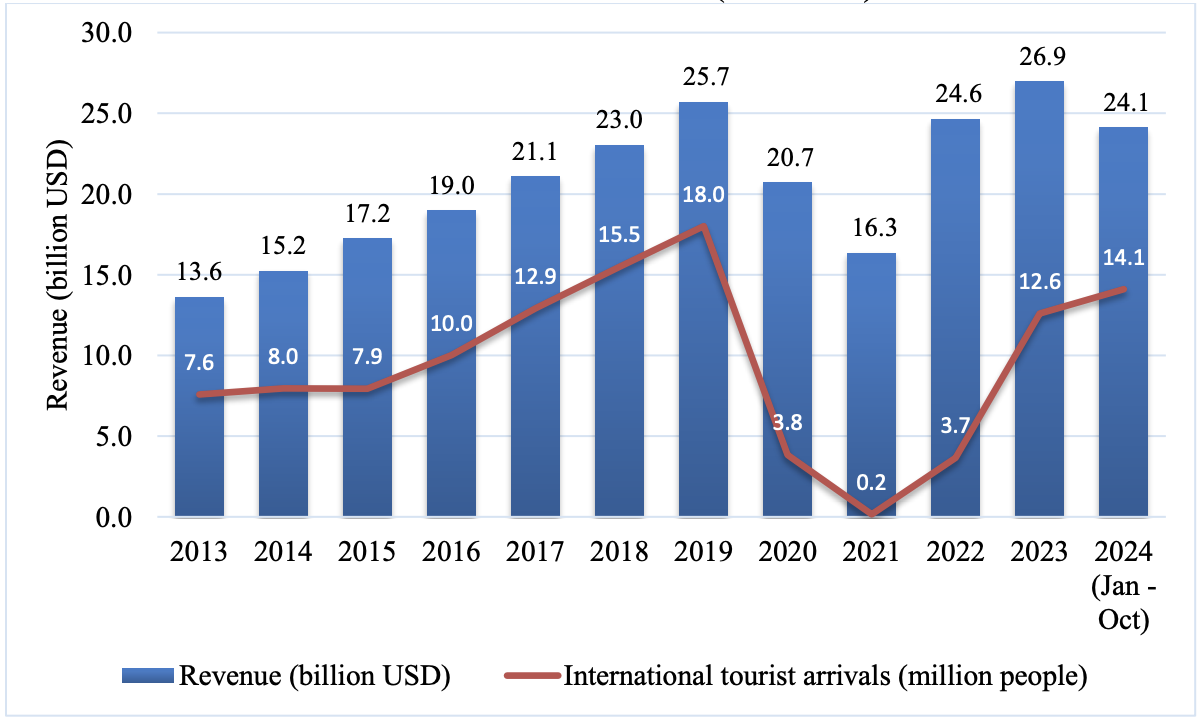
\includegraphics[width=15cm]{Images/resindus.png}
%     \caption{Doanh thu từ Dịch vụ Lưu trú, Ăn uống và Số lượng Du khách Quốc tế từ năm 2013 đến năm 2024. Nguồn: Post calculations; Vietnam’s General Statistics Office.}
%     \label{fig:enter-label}
% \end{figure}

% Trong bối cảnh công nghệ số ngày càng phát triển mạnh mẽ, việc áp dụng các giải pháp công nghệ vào quản lý và vận hành doanh nghiệp không chỉ là xu hướng mà còn là yếu tố quan trọng giúp nâng cao hiệu quả hoạt động và cải thiện trải nghiệm khách hàng. Đặc biệt, đối với ngành dịch vụ ăn uống, đặc biệt là các nhà hàng, việc quản lý quy trình đặt món và phục vụ khách hàng có thể gặp nhiều khó khăn và thách thức do tính chất phức tạp của công việc, cũng như yêu cầu phải đáp ứng nhu cầu đa dạng của khách hàng. \\

% Phương pháp quản lý truyền thống, dựa chủ yếu vào ghi chép thủ công và giao tiếp trực tiếp, đã bộc lộ nhiều hạn chế, chẳng hạn như dễ mắc sai sót, khó theo dõi lịch sử đặt món và tốn thời gian trong quá trình vận hành. Những vấn đề này không chỉ làm giảm hiệu quả công việc mà còn ảnh hưởng xấu đến trải nghiệm của khách hàng, đặc biệt là trong môi trường cạnh tranh ngày càng gay gắt trong ngành. \\

% Dự án này được triển khai nhằm giải quyết những vấn đề đó thông qua việc xây dựng một hệ thống quản lý đặt món hiện đại. Hệ thống này không chỉ tự động hóa các quy trình từ việc đặt món, quản lý đơn hàng đến thanh toán, mà còn giúp nhà hàng dễ dàng mở rộng các tính năng như quản lý kho, tối ưu hóa lịch làm việc của nhân viên và phân tích doanh thu. \\

% Việc triển khai hệ thống quản lý đặt món hiện đại sẽ mang lại nhiều lợi ích cho cả khách hàng và nhà hàng. Khách hàng có thể dễ dàng tiếp cận thực đơn, đặt món nhanh chóng và thanh toán tiện lợi. Còn đối với nhà hàng, việc này giúp nâng cao hiệu quả vận hành, giảm thiểu chi phí và tối ưu hóa nguồn lực. Đây không chỉ là một bước tiến quan trọng trong việc cải thiện quy trình kinh doanh mà còn là nền tảng giúp các nhà hàng sẵn sàng hội nhập và phát triển bền vững trong kỷ nguyên số. \\



% \subsubsection{Chuyển đổi số trong ngành công nghiệp nhà hàng ở Việt Nam}
% Sự tích hợp công nghệ đã và đang đóng vai trò then chốt trong việc thay đổi sâu sắc ngành công nghiệp nhà hàng, mang đến những bước đột phá trong hoạt động và trải nghiệm khách hàng. Các công nghệ hiện đại không chỉ giúp cải thiện hiệu quả vận hành mà còn tối ưu hóa các quy trình và nâng cao chất lượng dịch vụ. Dưới đây là những công nghệ nổi bật đang làm thay đổi ngành nhà hàng:
% \begin{enumerate}
%     \item \textbf{Hệ Thống POS (Điểm Bán Hàng)}: Các hệ thống POS hiện nay không chỉ đơn giản là máy tính tiền mà đã phát triển thành những giải pháp toàn diện, hỗ trợ các nhà hàng trong việc quản lý đơn hàng, theo dõi tồn kho và phân tích xu hướng bán hàng. Với sự hỗ trợ của POS, các chủ nhà hàng có thể đưa ra các quyết định sáng suốt, tối ưu hóa các hoạt động quản lý và tăng cường lợi thế cạnh tranh, giúp duy trì sự phát triển bền vững trong một ngành công nghiệp luôn thay đổi.
%     % \item \textbf{Trí Tuệ Nhân Tạo (AI)}: AI đang cách mạng hóa ngành nhà hàng bằng cách tự động hóa nhiều quy trình, từ giao đồ ăn cho đến việc thanh toán hóa đơn. Các công cụ AI giúp nhà hàng tối ưu hóa thực đơn, điều chỉnh giá cả và giảm thiểu lãng phí thực phẩm thông qua việc quản lý lịch trình sản xuất. Hơn thế nữa, AI còn góp phần nâng cao trải nghiệm khách hàng khi có thể hỗ trợ quản lý đặt chỗ, trả lời các câu hỏi của khách hàng một cách nhanh chóng và chính xác, từ đó giúp tăng mức độ hài lòng của khách hàng.
%     \item \textbf{Đặt Món Trực Tuyến (Online)}: Thói quen tiêu dùng tại Việt Nam đang thay đổi mạnh mẽ với sự ưa chuộng các giao dịch số và thanh toán trực tuyến. Dịch vụ giao đồ ăn trực tuyến đã trở thành một phần không thể thiếu trong thói quen của nhiều người, đặc biệt là ở các thành phố lớn. Theo thống kê, trong năm 2023, chi tiêu của người tiêu dùng Việt Nam cho dịch vụ giao đồ ăn tăng 30\%, đạt mức 1,4 tỷ USD, mức tăng trưởng cao nhất trong khu vực Đông Nam Á \cite{USDA}. Các nhà hàng đang tận dụng mạnh mẽ kênh giao đồ ăn trực tuyến để thúc đẩy doanh thu và thu hút khách hàng mới. Ví dụ, KFC đã mở thêm các cửa hàng ảo trên các nền tảng thương mại điện tử như Shopee Food và Grab Food, đồng thời sử dụng TikTok để livestream và cung cấp các ưu đãi hấp dẫn, gia tăng sự tương tác với khách hàng và đảm bảo giao hàng nhanh chóng trong vòng một giờ. 

% \end{enumerate}

% \begin{figure}[H]
%     \centering
%     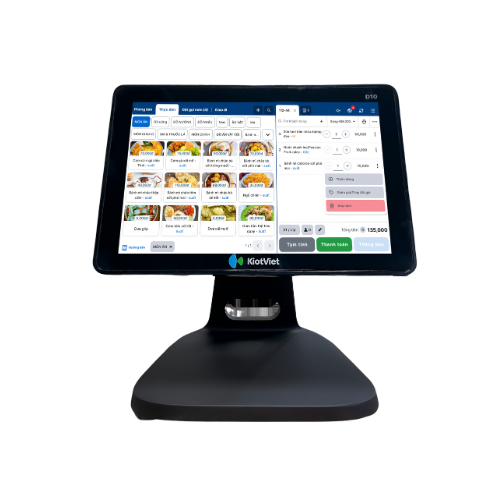
\includegraphics[width=15cm]{Images/kiosViet.png}
%     \caption{Máy POS KiotViet D10. Nguồn: \href{https://www.kiotviet.vn/top-4-may-tinh-tien-cho-quan-an-quan-cafe-tot-nhat-hien-nay/}{kiotviet.vn}}
% \end{figure}

% Mặc dù công nghệ đã mang lại những bước tiến vượt bậc, ngành nhà hàng vẫn phải đối mặt với một số thách thức lớn. Lạm phát và chi phí thực phẩm tăng cao đang tạo ra áp lực nặng nề, khiến hơn 30.000 cơ sở nhà hàng phải đóng cửa trong nửa đầu năm 2024 \cite{USDA}. Thêm vào đó, thiếu hụt lao động, đặc biệt là nhân viên có tay nghề cao, và các vấn đề liên quan đến chuỗi cung ứng cũng khiến các nhà hàng gặp khó khăn trong việc duy trì hoạt động hiệu quả. Gián đoạn toàn cầu ảnh hưởng đến nguồn cung nguyên liệu, làm gia tăng chi phí và giảm tính linh hoạt trong quản lý. Tuy nhiên, những thách thức này cũng tạo cơ hội lớn để đổi mới và cải tiến. Bên cạnh đó, sự phát triển mạnh mẽ của các nền tảng giao đồ ăn trực tuyến và thương mại điện tử đã mở ra những kênh doanh thu mới, giúp ngành nhà hàng không chỉ duy trì mà còn gia tăng sự phát triển. \\

% Nhờ vào sự cải tiến liên tục trong công nghệ, ngành nhà hàng tại Việt Nam đã và đang chứng kiến những bước tiến vượt bậc trong việc nâng cao chất lượng dịch vụ và cải thiện trải nghiệm khách hàng. Các giải pháp như hệ thống POS hiện đại, ứng dụng di động để đặt món và theo dõi giao hàng, cũng như sự tích hợp trí tuệ nhân tạo đã giúp các nhà hàng hoạt động hiệu quả hơn và đáp ứng nhu cầu ngày càng cao của khách hàng. Sự gia tăng dịch vụ giao đồ ăn trực tuyến càng làm cho việc ăn uống trở nên tiện lợi hơn, đặc biệt là ở các khu vực đô thị, khi mà khách hàng có thể dễ dàng đặt món và thanh toán qua các ví điện tử. Các nhà hàng không chỉ đơn giản là cung cấp thực phẩm, mà còn đang mang lại trải nghiệm mua sắm thuận tiện, nhanh chóng và an toàn cho khách hàng. \\

% Ngành công nghiệp nhà hàng tại Việt Nam hiện nay đang ở một ngã rẽ quan trọng, khi công nghệ đóng vai trò trung tâm trong sự phát triển của ngành. Mặc dù vẫn còn những thách thức đáng kể, việc áp dụng công nghệ chiến lược mang lại cơ hội lớn cho các doanh nghiệp nhà hàng. Tích hợp các hệ thống POS tiên tiến, ứng dụng di động giúp tối ưu hóa các hoạt động, tạo ra những cải tiến đáng kể trong trải nghiệm khách hàng. Trong khi thị trường tiếp tục phát triển, việc ứng dụng công nghệ sẽ là yếu tố then chốt giúp các nhà hàng duy trì sự cạnh tranh và đáp ứng nhu cầu thay đổi của khách hàng trong kỷ nguyên số.








\subsection{Giới thiệu đề tài}

Tính đến năm 2023, ngành dịch vụ thực phẩm (bao gồm khách sạn, nhà hàng và dịch vụ thể chế) đã đạt tổng giá trị 26,9 tỷ USD, với mức tăng trưởng 14,7\%. Mặc dù phải đối mặt với nhiều thách thức như lạm phát, chi phí vận hành tăng cao và sự cạnh tranh khốc liệt, ngành này đã phục hồi mạnh mẽ và gần như đạt doanh thu tương đương với thời kỳ trước đại dịch. Trong nửa đầu năm 2024, doanh thu từ dịch vụ lưu trú, thực phẩm và đồ uống đạt 24,1 tỷ USD, tăng 12,5\% so với cùng kỳ năm trước \cite{USDA}. 

\begin{figure}[H]
    \centering
    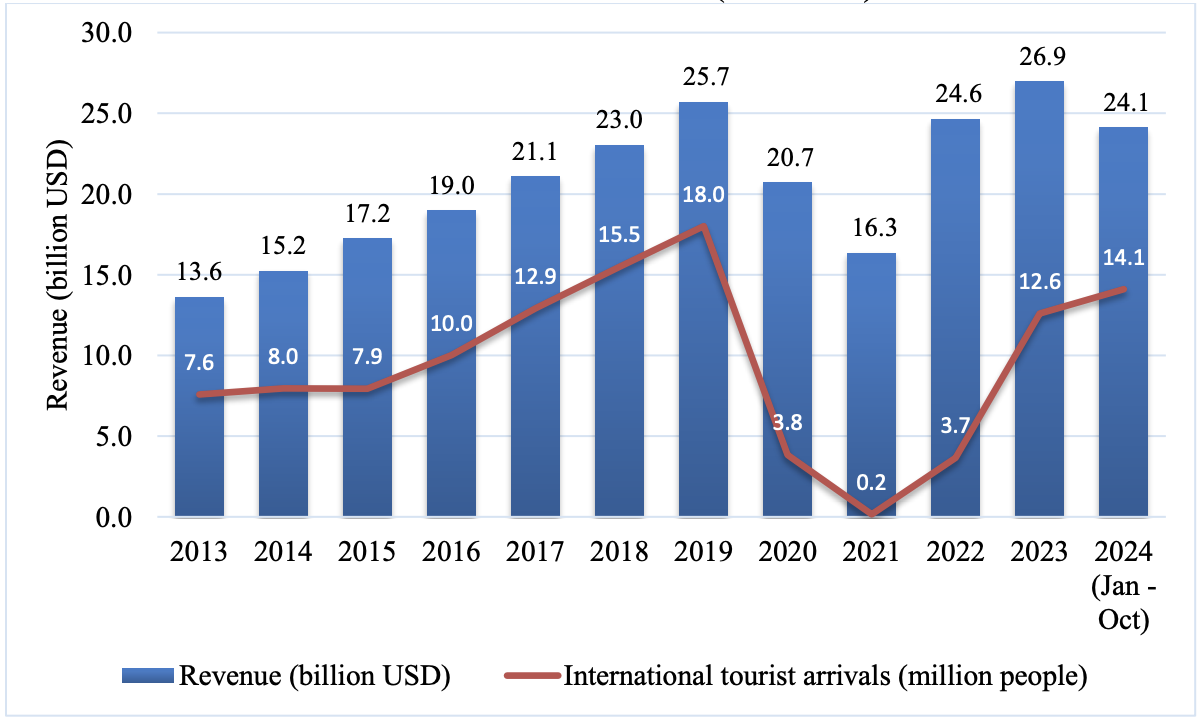
\includegraphics[width=15cm]{Images/resindus.png}
    \caption{Doanh thu từ Dịch vụ Lưu trú, Ăn uống và Số lượng Du khách Quốc tế từ năm 2013 đến năm 2024. Nguồn: Post calculations; Vietnam’s General Statistics Office.}
    \label{fig:enter-label}
\end{figure}

Trong bối cảnh công nghệ số ngày càng phát triển mạnh mẽ, việc áp dụng các giải pháp công nghệ vào quản lý và vận hành doanh nghiệp không chỉ là xu hướng mà còn là yếu tố quan trọng giúp nâng cao hiệu quả hoạt động và cải thiện trải nghiệm khách hàng. Đặc biệt, đối với ngành dịch vụ ăn uống, đặc biệt là các nhà hàng, việc quản lý quy trình đặt món và phục vụ khách hàng có thể gặp nhiều khó khăn và thách thức do tính chất phức tạp của công việc, cũng như yêu cầu phải đáp ứng nhu cầu đa dạng của khách hàng.

Phương pháp quản lý truyền thống, dựa chủ yếu vào ghi chép thủ công và giao tiếp trực tiếp, đã bộc lộ nhiều hạn chế, chẳng hạn như dễ mắc sai sót, khó theo dõi lịch sử đặt món và tốn thời gian trong quá trình vận hành. Những vấn đề này không chỉ làm giảm hiệu quả công việc mà còn ảnh hưởng xấu đến trải nghiệm của khách hàng, đặc biệt là trong môi trường cạnh tranh ngày càng gay gắt trong ngành.

Sự tích hợp công nghệ đã và đang đóng vai trò then chốt trong việc thay đổi sâu sắc ngành công nghiệp nhà hàng, mang đến những bước đột phá trong hoạt động và trải nghiệm khách hàng. Các công nghệ hiện đại không chỉ giúp cải thiện hiệu quả vận hành mà còn tối ưu hóa các quy trình và nâng cao chất lượng dịch vụ. Dưới đây là những công nghệ nổi bật đang làm thay đổi ngành nhà hàng:
\begin{enumerate}
    \item \textbf{Hệ Thống POS (Điểm Bán Hàng)}: Các hệ thống POS hiện nay không chỉ đơn giản là máy tính tiền mà đã phát triển thành những giải pháp toàn diện, hỗ trợ các nhà hàng trong việc quản lý đơn hàng, theo dõi tồn kho và phân tích xu hướng bán hàng. Với sự hỗ trợ của POS, các chủ nhà hàng có thể đưa ra các quyết định sáng suốt, tối ưu hóa các hoạt động quản lý và tăng cường lợi thế cạnh tranh, giúp duy trì sự phát triển bền vững trong một ngành công nghiệp luôn thay đổi.
    \item \textbf{Đặt Món Trực Tuyến (Online)}: Thói quen tiêu dùng tại Việt Nam đang thay đổi mạnh mẽ với sự ưa chuộng các giao dịch số và thanh toán trực tuyến. Dịch vụ giao đồ ăn trực tuyến đã trở thành một phần không thể thiếu trong thói quen của nhiều người, đặc biệt là ở các thành phố lớn. Theo thống kê, trong năm 2023, chi tiêu của người tiêu dùng Việt Nam cho dịch vụ giao đồ ăn tăng 30\%, đạt mức 1,4 tỷ USD, mức tăng trưởng cao nhất trong khu vực Đông Nam Á \cite{USDA}. Các nhà hàng đang tận dụng mạnh mẽ kênh giao đồ ăn trực tuyến để thúc đẩy doanh thu và thu hút khách hàng mới. Ví dụ, KFC đã mở thêm các cửa hàng ảo trên các nền tảng thương mại điện tử như Shopee Food và Grab Food, đồng thời sử dụng TikTok để livestream và cung cấp các ưu đãi hấp dẫn, gia tăng sự tương tác với khách hàng và đảm bảo giao hàng nhanh chóng trong vòng một giờ.
\end{enumerate}

\begin{figure}[H]
    \centering
    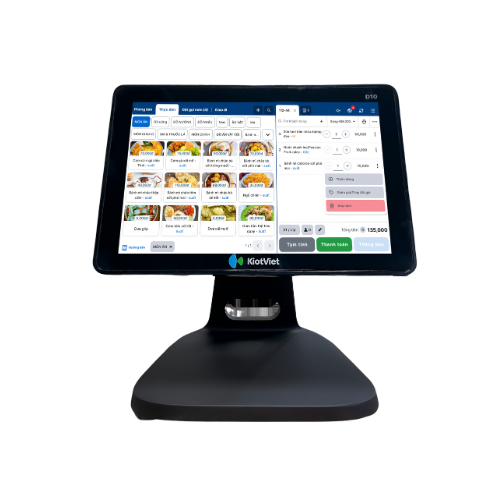
\includegraphics[width=10cm]{Images/kiosViet.png}
    \caption{Máy POS KiotViet D10. Nguồn: \href{https://www.kiotviet.vn/top-4-may-tinh-tien-cho-quan-an-quan-cafe-tot-nhat-hien-nay/}{kiotviet.vn}}
\end{figure}

Mặc dù công nghệ đã mang lại những bước tiến vượt bậc, ngành nhà hàng vẫn phải đối mặt với một số thách thức lớn. Lạm phát và chi phí thực phẩm tăng cao đang tạo ra áp lực nặng nề, khiến hơn 30.000 cơ sở nhà hàng phải đóng cửa trong nửa đầu năm 2024 \cite{USDA}. Thêm vào đó, thiếu hụt lao động, đặc biệt là nhân viên có tay nghề cao, và các vấn đề liên quan đến chuỗi cung ứng cũng khiến các nhà hàng gặp khó khăn trong việc duy trì hoạt động hiệu quả. Gián đoạn toàn cầu ảnh hưởng đến nguồn cung nguyên liệu, làm gia tăng chi phí và giảm tính linh hoạt trong quản lý. Tuy nhiên, những thách thức này cũng tạo cơ hội lớn để đổi mới và cải tiến. Bên cạnh đó, sự phát triển mạnh mẽ của các nền tảng giao đồ ăn trực tuyến và thương mại điện tử đã mở ra những kênh doanh thu mới, giúp ngành nhà hàng không chỉ duy trì mà còn gia tăng sự phát triển.

Dự án này được triển khai nhằm giải quyết những vấn đề đó thông qua việc xây dựng một hệ thống quản lý đặt món hiện đại. Hệ thống này không chỉ tự động hóa các quy trình từ việc đặt món, quản lý đơn hàng đến thanh toán, mà còn giúp nhà hàng dễ dàng mở rộng các tính năng như tối ưu hóa lịch làm việc của nhân viên và phân tích doanh thu.

Việc triển khai hệ thống quản lý đặt món hiện đại sẽ mang lại nhiều lợi ích cho cả khách hàng và nhà hàng. Khách hàng có thể dễ dàng tiếp cận thực đơn, đặt món nhanh chóng và thanh toán tiện lợi. Còn đối với nhà hàng, việc này giúp nâng cao hiệu quả vận hành, giảm thiểu chi phí và tối ưu hóa nguồn lực. Đây không chỉ là một bước tiến quan trọng trong việc cải thiện quy trình kinh doanh mà còn là nền tảng giúp các nhà hàng sẵn sàng hội nhập và phát triển bền vững trong kỷ nguyên số.

Nhờ vào sự cải tiến liên tục trong công nghệ, ngành nhà hàng tại Việt Nam đã và đang chứng kiến những bước tiến vượt bậc trong việc nâng cao chất lượng dịch vụ và cải thiện trải nghiệm khách hàng. Các giải pháp như hệ thống POS hiện đại, ứng dụng di động để đặt món và theo dõi giao hàng đã giúp các nhà hàng hoạt động hiệu quả hơn và đáp ứng nhu cầu ngày càng cao của khách hàng. Sự gia tăng dịch vụ giao đồ ăn trực tuyến càng làm cho việc ăn uống trở nên tiện lợi hơn, đặc biệt là ở các khu vực đô thị, khi mà khách hàng có thể dễ dàng đặt món và thanh toán qua các ví điện tử. Các nhà hàng không chỉ đơn giản là cung cấp thực phẩm, mà còn đang mang lại trải nghiệm mua sắm thuận tiện, nhanh chóng và an toàn cho khách hàng.

Ngành công nghiệp nhà hàng tại Việt Nam hiện nay đang ở một ngã rẽ quan trọng, khi công nghệ đóng vai trò trung tâm trong sự phát triển của ngành. Mặc dù vẫn còn những thách thức đáng kể, việc áp dụng công nghệ chiến lược mang lại cơ hội lớn cho các doanh nghiệp nhà hàng. Tích hợp các hệ thống POS tiên tiến, ứng dụng di động giúp tối ưu hóa các hoạt động, tạo ra những cải tiến đáng kể trong trải nghiệm khách hàng. Trong khi thị trường tiếp tục phát triển, việc ứng dụng công nghệ sẽ là yếu tố then chốt giúp các nhà hàng duy trì sự cạnh tranh và đáp ứng nhu cầu thay đổi của khách hàng trong kỷ nguyên số.


% % \subsection{Động lực}

% % Việc phát triển hệ thống quản lý đặt món trong nhà hàng xuất phát từ nhu cầu thực tế và những lợi ích mà nó mang lại:

% % \begin{enumerate}
% %     \item Xu hướng chuyển đổi số trong ngành dịch vụ ăn uống: Ngày nay, việc ứng dụng công nghệ vào các lĩnh vực kinh doanh không chỉ là một lựa chọn mà đã trở thành một yêu cầu bắt buộc. Các nhà hàng cần áp dụng các giải pháp hiện đại để nâng cao hiệu quả hoạt động và mang lại trải nghiệm tốt hơn cho khách hàng.

% %     \item Tăng trải nghiệm khách hàng: Một hệ thống quản lý đặt món tự động giúp khách hàng dễ dàng tiếp cận thực đơn, tùy chỉnh các lựa chọn, đặt món và thanh toán nhanh chóng. Điều này góp phần tạo ấn tượng tích cực và giữ chân khách hàng lâu dài.

% %     \item Giảm áp lực cho nhân viên: Nhân viên nhà hàng thường gặp khó khăn khi phải xử lý nhiều đơn hàng cùng lúc, đặc biệt vào giờ cao điểm. Hệ thống tự động hóa giúp giảm thiểu sai sót và tăng năng suất làm việc của nhân viên.

% %     \item Tăng tính cạnh tranh trên thị trường: Với sự phát triển của các mô hình nhà hàng thông minh, việc áp dụng công nghệ không chỉ giúp tối ưu hóa hoạt động mà còn tạo lợi thế cạnh tranh với các đối thủ.

% %     \item Hỗ trợ quản lý hiệu quả: Một hệ thống hiện đại không chỉ dừng lại ở việc quản lý đặt món mà còn cung cấp các công cụ phân tích, báo cáo giúp nhà quản lý đưa ra các quyết định kinh doanh chiến lược dựa trên dữ liệu thực tế.
% % \end{enumerate}

% % Động lực từ thực tiễn và xu hướng công nghệ chính là yếu tố thúc đẩy việc thực hiện đề tài này, nhằm giải quyết các vấn đề hiện tại và hướng đến sự phát triển bền vững.

% \subsection{Động lực}

% Việc phát triển hệ thống quản lý đặt món trong nhà hàng xuất phát từ nhu cầu thực tế và những lợi ích mà nó mang lại, đặc biệt trong bối cảnh ngành công nghiệp nhà hàng tại Việt Nam đang chuyển đổi số mạnh mẽ như đã đề cập:

% \begin{enumerate}
%     \item \textbf{Xu hướng chuyển đổi số trong ngành dịch vụ ăn uống}: Như đã trình bày, sự tích hợp công nghệ, chẳng hạn như hệ thống POS và dịch vụ đặt món trực tuyến, đã trở thành yếu tố then chốt giúp nhà hàng nâng cao hiệu quả và đáp ứng nhu cầu khách hàng. Việc áp dụng một hệ thống quản lý đặt món hiện đại là một bước đi cần thiết để theo kịp xu hướng này.
    
%     \item \textbf{Tăng trải nghiệm khách hàng}: Hệ thống tự động hóa giúp khách hàng dễ dàng tiếp cận thực đơn, tùy chỉnh món ăn, đặt hàng nhanh chóng và thanh toán tiện lợi qua các nền tảng số, như đã thấy trong sự phát triển của dịch vụ giao đồ ăn trực tuyến. Điều này không chỉ cải thiện trải nghiệm mà còn xây dựng lòng trung thành của khách hàng.
    
%     \item \textbf{Giảm áp lực cho nhân viên}: Trong môi trường cạnh tranh và áp lực cao của ngành nhà hàng, nhân viên thường phải xử lý nhiều đơn hàng cùng lúc. Hệ thống quản lý đặt món giúp giảm thiểu sai sót, tối ưu hóa quy trình phục vụ, từ đó nâng cao năng suất làm việc, như đã đề cập trong các hạn chế của phương pháp quản lý truyền thống.
    
%     \item \textbf{Tăng tính cạnh tranh trên thị trường}: Với sự gia tăng của các mô hình nhà hàng thông minh và kênh giao đồ ăn trực tuyến như Shopee Food hay Grab Food, việc áp dụng công nghệ giúp nhà hàng tạo lợi thế cạnh tranh, thu hút khách hàng mới và duy trì vị thế trên thị trường.
    
%     \item \textbf{Hỗ trợ quản lý hiệu quả}: Hệ thống không chỉ tự động hóa quy trình đặt món mà còn cung cấp các công cụ phân tích doanh thu, quản lý kho và tối ưu hóa lịch làm việc, giúp nhà quản lý đưa ra quyết định chiến lược dựa trên dữ liệu thực tế, như vai trò của hệ thống POS đã được đề cập.
% \end{enumerate}

% Động lực từ nhu cầu thực tiễn, xu hướng công nghệ và những thách thức trong vận hành nhà hàng chính là yếu tố thúc đẩy việc thực hiện đề tài này, nhằm mang lại giải pháp toàn diện và bền vững.



\subsection{Động lực}

Việc nghiên cứu và phát triển một hệ thống quản lý đặt món hiện đại cho nhà hàng không chỉ là một đề xuất cải tiến mà còn xuất phát từ những động lực cấp thiết và cơ hội chiến lược, bám sát vào thực trạng và xu hướng của ngành dịch vụ ẩm thực tại Việt Nam như đã được phân tích chi tiết trong phần giới thiệu:

\begin{enumerate}
    \item \textbf{Yêu cầu cấp bách từ làn sóng Chuyển đổi số trong ngành Food\&Beverage:} Như đã nêu, ngành dịch vụ thực phẩm Việt Nam (đạt 26,9 tỷ USD năm 2023) đang chứng kiến sự chuyển mình mạnh mẽ nhờ công nghệ. Sự phổ biến của các hệ thống POS tiên tiến và sự bùng nổ của thị trường đặt món trực tuyến (đạt 1,4 tỷ USD, tăng 30\% năm 2023 \cite{USDA}) không chỉ là xu hướng mà đã trở thành một phần quan trọng trong mô hình kinh doanh hiện đại. Việc không tích hợp công nghệ, cụ thể là một hệ thống quản lý đặt món hiệu quả, đồng nghĩa với việc nhà hàng tự đặt mình vào thế bất lợi, có nguy cơ bị tụt hậu so với các đối thủ đang nhanh chóng thích nghi và khai thác lợi ích từ công nghệ số. Do đó, phát triển hệ thống này là một bước đi tất yếu để hòa nhập và cạnh tranh.

    \item \textbf{Khắc phục những hạn chế cố hữu của phương pháp quản lý truyền thống:} Quy trình vận hành dựa trên ghi chép thủ công và giao tiếp trực tiếp, như đã đề cập, tiềm ẩn nhiều rủi ro: sai sót trong ghi nhận đơn hàng, nhầm lẫn trong quá trình chuyển thông tin đến bếp, khó khăn trong việc theo dõi lịch sử và sở thích khách hàng, và lãng phí thời gian của cả nhân viên lẫn khách hàng. Những sai sót này không chỉ gây thất thoát doanh thu mà còn làm tổn hại đến uy tín thương hiệu và sự hài lòng của khách hàng. Một hệ thống quản lý đặt món tự động hóa sẽ giải quyết các nút thắt này, đảm bảo tính chính xác, minh bạch và hiệu quả cho toàn bộ quy trình từ lúc khách chọn món đến khi hoàn tất thanh toán.

    \item \textbf{Nâng tầm trải nghiệm khách hàng trong kỷ nguyên số và tiện ích:} Khách hàng hiện đại, đặc biệt tại các đô thị, ngày càng đề cao sự tiện lợi, tốc độ và khả năng kiểm soát trong trải nghiệm dịch vụ. Họ đã quen với các giao dịch số và mong muốn quy trình đặt món tại nhà hàng cũng mượt mà như vậy. Hệ thống quản lý đặt món hiện đại đáp ứng kỳ vọng này bằng cách cho phép khách hàng dễ dàng xem thực đơn (có thể kèm hình ảnh, mô tả chi tiết), tùy chỉnh món ăn theo sở thích cá nhân, đặt hàng nhanh chóng (có thể ngay tại bàn qua thiết bị di động hoặc kiosk) và thanh toán thuận tiện qua nhiều hình thức điện tử. Việc giảm thiểu thời gian chờ đợi, đảm bảo đơn hàng chính xác và mang lại sự chủ động cho khách hàng chính là yếu tố then chốt để tạo ấn tượng tích cực, xây dựng lòng trung thành và khuyến khích họ quay trở lại.

    \item \textbf{Tối ưu hóa hiệu quả vận hành và tăng cường năng lực cạnh tranh trong bối cảnh thách thức:} Ngành nhà hàng đang đối mặt với áp lực không nhỏ từ lạm phát, chi phí nguyên liệu và vận hành tăng cao (thể hiện qua con số hơn 30.000 cơ sở đóng cửa \cite{USDA}), cùng với tình trạng thiếu hụt lao động có kỹ năng. Trong bối cảnh đó, việc tối ưu hóa nguồn lực và quy trình là yếu tố sống còn. Hệ thống quản lý đặt món giúp giảm tải đáng kể công việc thủ công cho nhân viên phục vụ và thu ngân, giảm thiểu sai sót do con người, cho phép phân bổ nhân sự hiệu quả hơn. Quan trọng hơn, hệ thống cung cấp dữ liệu vận hành chi tiết (tương tự vai trò phân tích của POS), giúp nhà quản lý nắm bắt xu hướng tiêu dùng, quản lý tốt hơn, đưa ra các quyết định về giá cả, thực đơn và chiến lược kinh doanh dựa trên bằng chứng cụ thể, từ đó nâng cao hiệu quả và tạo lợi thế cạnh tranh sắc bén.
\end{enumerate}

Tóm lại, động lực cốt lõi thúc đẩy việc thực hiện đề tài này là sự cộng hưởng mạnh mẽ giữa nhu cầu giải quyết các bài toán thực tiễn trong quản lý nhà hàng, yêu cầu phải bắt kịp và tận dụng xu thế chuyển đổi số không thể đảo ngược, cùng với khát vọng nâng cao chất lượng dịch vụ, tối ưu hóa hiệu quả hoạt động và xây dựng lợi thế cạnh tranh bền vững cho các doanh nghiệp trong ngành ẩm thực Việt Nam.
% % \subsection{Thách thức}
% % Trong quá trình phát triển và triển khai hệ thống quản lý đặt món cho nhà hàng, có thể đối mặt với nhiều thách thức, bao gồm:

% % \begin{enumerate}
% %     \item Đáp ứng đa dạng nhu cầu người dùng: Khách hàng, nhân viên phục vụ, quản lý chi nhánh, và quản lý tổng đều có các yêu cầu sử dụng khác nhau. Thiết kế hệ thống phải đảm bảo dễ sử dụng cho khách hàng, đồng thời cung cấp đủ công cụ và dữ liệu cho quản lý và nhân viên.

% %     \item Tích hợp với cơ sở hạ tầng hiện có: Nhiều nhà hàng đã có hệ thống quản lý cơ bản hoặc sử dụng các phần mềm khác. Việc tích hợp hệ thống mới với các công cụ hiện tại, như máy in hóa đơn, phần mềm kế toán hoặc thiết bị quét QR, là một thách thức cần giải quyết.

% %     \item Quản lý dữ liệu lớn: Khi hệ thống hoạt động tại nhiều chi nhánh với số lượng khách hàng lớn, việc lưu trữ, xử lý và bảo mật dữ liệu trở thành một bài toán quan trọng, đặc biệt đối với thông tin cá nhân và thanh toán.

% %     \item Bảo mật thông tin: Với việc tích hợp thanh toán qua QR hoặc các hình thức điện tử, việc đảm bảo an toàn dữ liệu giao dịch và thông tin khách hàng là một ưu tiên hàng đầu, đồng thời là một thách thức lớn trước các nguy cơ tấn công mạng.

% %     \item Đào tạo và thay đổi thói quen người dùng: Nhân viên và khách hàng có thể chưa quen với việc sử dụng công nghệ mới. Điều này đòi hỏi một quá trình đào tạo bài bản và hỗ trợ liên tục để đảm bảo mọi người đều sử dụng hệ thống hiệu quả.

% %     \item Quản lý lỗi và vận hành liên tục: Hệ thống phải hoạt động ổn định và có cơ chế xử lý lỗi nhanh chóng, đặc biệt trong các giờ cao điểm. Bất kỳ sự cố nào cũng có thể ảnh hưởng đến trải nghiệm khách hàng và hoạt động của nhà hàng.
% % \end{enumerate}

% % Những thách thức này đòi hỏi nhóm phải có kế hoạch chi tiết, giải pháp linh hoạt, ... để đảm bảo hệ thống hoạt động hiệu quả và mang lại giá trị cao nhất.


% \subsection{Thách thức}

% Trong quá trình phát triển và triển khai hệ thống quản lý đặt món, nhóm phải đối mặt với nhiều thách thức, đặc biệt khi liên kết với các vấn đề và giải pháp đã nêu trong phần giới thiệu:

% \begin{enumerate}
%     \item \textbf{Đáp ứng đa dạng nhu cầu người dùng}: Như đã đề cập, khách hàng yêu cầu trải nghiệm tiện lợi, trong khi nhà quản lý cần dữ liệu phân tích chi tiết và nhân viên cần giao diện dễ sử dụng. Thiết kế hệ thống phải cân bằng giữa tính đơn giản cho khách hàng và tính năng chuyên sâu cho quản lý, đảm bảo đáp ứng các nhu cầu đa dạng.
    
%     \item \textbf{Tích hợp với cơ sở hạ tầng hiện có}: Nhiều nhà hàng tại Việt Nam đã sử dụng các hệ thống POS hoặc phần mềm quản lý cơ bản, như KiotViet D10. Việc tích hợp hệ thống mới với các thiết bị hiện tại, chẳng hạn như máy in hóa đơn hoặc phần mềm kế toán, đòi hỏi sự tương thích cao để tránh gián đoạn vận hành.
    
%     \item \textbf{Quản lý dữ liệu lớn}: Với sự gia tăng giao dịch qua các nền tảng số, như dịch vụ giao đồ ăn trực tuyến, hệ thống cần xử lý và lưu trữ khối lượng dữ liệu lớn từ nhiều chi nhánh, đồng thời đảm bảo hiệu suất và bảo mật thông tin khách hàng.
    
%     \item \textbf{Bảo mật thông tin}: Trong bối cảnh thanh toán điện tử và giao dịch qua QR đang phổ biến, việc bảo vệ dữ liệu giao dịch và thông tin cá nhân trước các nguy cơ tấn công mạng là một thách thức lớn, đặc biệt khi ngành nhà hàng ngày càng phụ thuộc vào công nghệ số.
    
%     \item \textbf{Đào tạo và thay đổi thói quen người dùng}: Như đã nêu, phương pháp quản lý truyền thống vẫn phổ biến ở nhiều nhà hàng. Việc chuyển đổi sang hệ thống mới đòi hỏi đào tạo nhân viên và hướng dẫn khách hàng, đặc biệt với những người chưa quen sử dụng công nghệ, để đảm bảo hiệu quả sử dụng.
    
%     \item \textbf{Quản lý lỗi và vận hành liên tục}: Hệ thống phải hoạt động ổn định, đặc biệt trong giờ cao điểm, để tránh ảnh hưởng đến trải nghiệm khách hàng. Cơ chế xử lý lỗi nhanh chóng là cần thiết để duy trì hiệu quả vận hành, như yêu cầu về tính linh hoạt trong quản lý đã được đề cập.
% \end{enumerate}

% Những thách thức này đòi hỏi nhóm phát triển phải có kế hoạch chi tiết, giải pháp linh hoạt và sự phối hợp chặt chẽ để đảm bảo hệ thống không chỉ khắc phục các hạn chế hiện tại mà còn mang lại giá trị tối ưu cho ngành nhà hàng.

\subsection{Thách thức}

Mặc dù việc phát triển một hệ thống quản lý đặt món hiện đại mang lại nhiều lợi ích và phù hợp với xu hướng chuyển đổi số, quá trình xây dựng và triển khai hệ thống này cũng đối mặt với không ít thách thức đáng kể, đòi hỏi sự chuẩn bị kỹ lưỡng và giải pháp phù hợp:

\begin{enumerate}
    \item \textbf{Độ phức tạp về mặt kỹ thuật và tích hợp hệ thống:}
    Việc xây dựng một hệ thống toàn diện đòi hỏi xử lý nhiều nghiệp vụ phức tạp: quản lý thực đơn đa dạng (món lẻ, combo, tùy chọn gia giảm, topping), quản lý bàn và khu vực phục vụ, xử lý nhiều loại đơn hàng (tại chỗ, mang về, giao hàng), đồng bộ trạng thái đơn hàng giữa các bộ phận (phục vụ, bếp, thu ngân), và tích hợp với các hệ thống thanh toán khác nhau (tiền mặt, thẻ, ví điện tử).

    \item \textbf{Chi phí đầu tư ban đầu và chi phí duy trì:}
    Việc triển khai một hệ thống mới thường đi kèm với các chi phí duy trì định kỳ như nâng cấp hệ thống, phí dịch vụ lưu trữ (cloud) và hỗ trợ kỹ thuật.

    \item \textbf{Thiết kế trải nghiệm người dùng (UX/UI) tối ưu:}
    Hệ thống cần có giao diện thân thiện, trực quan và dễ sử dụng cho cả nhân viên và khách hàng (nếu có giao diện đặt món tự phục vụ). Một thiết kế UX/UI phức tạp, khó hiểu sẽ làm giảm hiệu quả công việc của nhân viên và gây khó chịu cho khách hàng, thậm chí dẫn đến việc từ bỏ sử dụng hệ thống. Việc cân bằng giữa tính năng đa dạng và sự đơn giản trong thiết kế, đồng thời đảm bảo tính nhất quán trên các nền tảng khác nhau (web, app, kiosk) là một thách thức không nhỏ.

    \item \textbf{Bảo mật dữ liệu và quyền riêng tư:}
    Hệ thống sẽ lưu trữ và xử lý nhiều dữ liệu nhạy cảm, bao gồm thông tin đơn hàng, dữ liệu bán hàng, thông tin cá nhân và lịch sử giao dịch của khách hàng, thông tin thanh toán. Việc đảm bảo an ninh, an toàn cho các dữ liệu này, chống lại các nguy cơ tấn công mạng, truy cập trái phép, mã hóa dữ liệu và tuân thủ các quy định pháp luật về bảo vệ dữ liệu cá nhân (như Nghị định 13/2023/NĐ-CP của Việt Nam) là một yêu cầu bắt buộc và là thách thức liên tục trong suốt vòng đời của hệ thống.

    % \item \textbf{Giới hạn về thời gian hoàn thành dự án:}
    % Việc phát triển một hệ thống phức tạp đòi hỏi thời gian nghiên cứu, thiết kế, lập trình, kiểm thử và triển khai kỹ lưỡng. Việc cân bằng giữa tốc độ phát triển và chất lượng sản phẩm, đồng thời quản lý hiệu quả các mốc thời gian và đối phó với những thay đổi yêu cầu phát sinh là một thách thức lớn đối với đội ngũ phát triển.

    % \item \textbf{Nguồn nhân lực phát triển và quản lý dự án:}
    % Việc xây dựng và duy trì kinh nghiệm về các công nghệ cần thiết (backend, frontend, database, mobile, DevOps, security) và hiểu biết về nghiệp vụ nhà hàng là một thách thức. Ngoài ra, việc quản lý dự án hiệu quả, điều phối công việc giữa các thành viên, và giao tiếp thông suốt cũng đóng vai trò quan trọng nhưng không hề dễ dàng.
\end{enumerate}

Việc nhận diện và có kế hoạch đối phó với những thách thức này ngay từ giai đoạn đầu của dự án là yếu tố then chốt để đảm bảo hệ thống quản lý đặt món được phát triển thành công, triển khai hiệu quả và mang lại giá trị thực sự cho nhà hàng.

% \subsection{Mục tiêu đề tài}

% Nhằm vượt qua những thách thức cố hữu và khai thác tối đa tiềm năng trong từng giai đoạn của hành trình khách hàng, nhóm nghiên cứu đã phát triển một ứng dụng tích hợp, được thiết kế chuyên biệt để nâng tầm trải nghiệm cho khách hàng, nhân viên và quản lý nhà hàng. Ứng dụng này tập trung vào việc cải thiện các điểm chạm then chốt trong hành trình khách hàng, tạo ra một quy trình liền mạch và hiệu quả hơn:
% \begin{enumerate}
%     \item Giai đoạn Cân nhắc (Consideration):     Ứng dụng cho phép khách hàng dễ dàng truy cập thực đơn trực tuyến chi tiết, hình ảnh chất lượng cao về món ăn và không gian nhà hàng, cũng như các đánh giá từ những khách hàng khác. Chức năng so sánh giá cả và tùy chọn tùy chỉnh món ăn giúp khách hàng đưa ra quyết định sáng suốt..
%     \item Giai đoạn Trải nghiệm (Experience): Ứng dụng cung cấp các tính năng hỗ trợ trong quá trình trải nghiệm tại nhà hàng, bao gồm một vài tính năng cơ bản như:
%         \begin{itemize}
%             \item \textit{Gọi món qua ứng dụng:} Khách hàng có thể dễ dàng xem thực đơn và gọi món trên điện thoại thông minh của mình.
%             \item \textit{Gửi yêu cầu trực tiếp đến nhân viên phục vụ:} Giúp tăng cường tương tác và giải quyết các vấn đề nhanh chóng.
%             \item \textit{Thu thập phản hồi thời gian thực:} Cho phép nhà hàng đánh giá và cải thiện chất lượng dịch vụ ngay lập tức.
%         \end{itemize}
%     \item Giai đoạn Thanh toán (Payment): Ứng dụng tích hợp nhiều phương thức thanh toán điện tử (thẻ tín dụng, ví điện tử), cho phép khách hàng thanh toán nhanh chóng và an toàn. Hóa đơn điện tử được tạo tự động và gửi trực tiếp đến khách hàng.
%     \item Giai đoạn Hậu trải nghiệm (Post-Experience): Ứng dụng hỗ trợ gửi email cảm ơn tự động, khuyến khích khách hàng để lại đánh giá và tham gia chương trình khách hàng thân thiết. Dữ liệu về lịch sử mua hàng và sở thích của khách hàng được sử dụng để cá nhân hóa các ưu đãi và khuyến mãi, tăng khả năng quay lại của khách hàng.

% \end{enumerate}

% \begin{figure}[H]
%     \centering
%     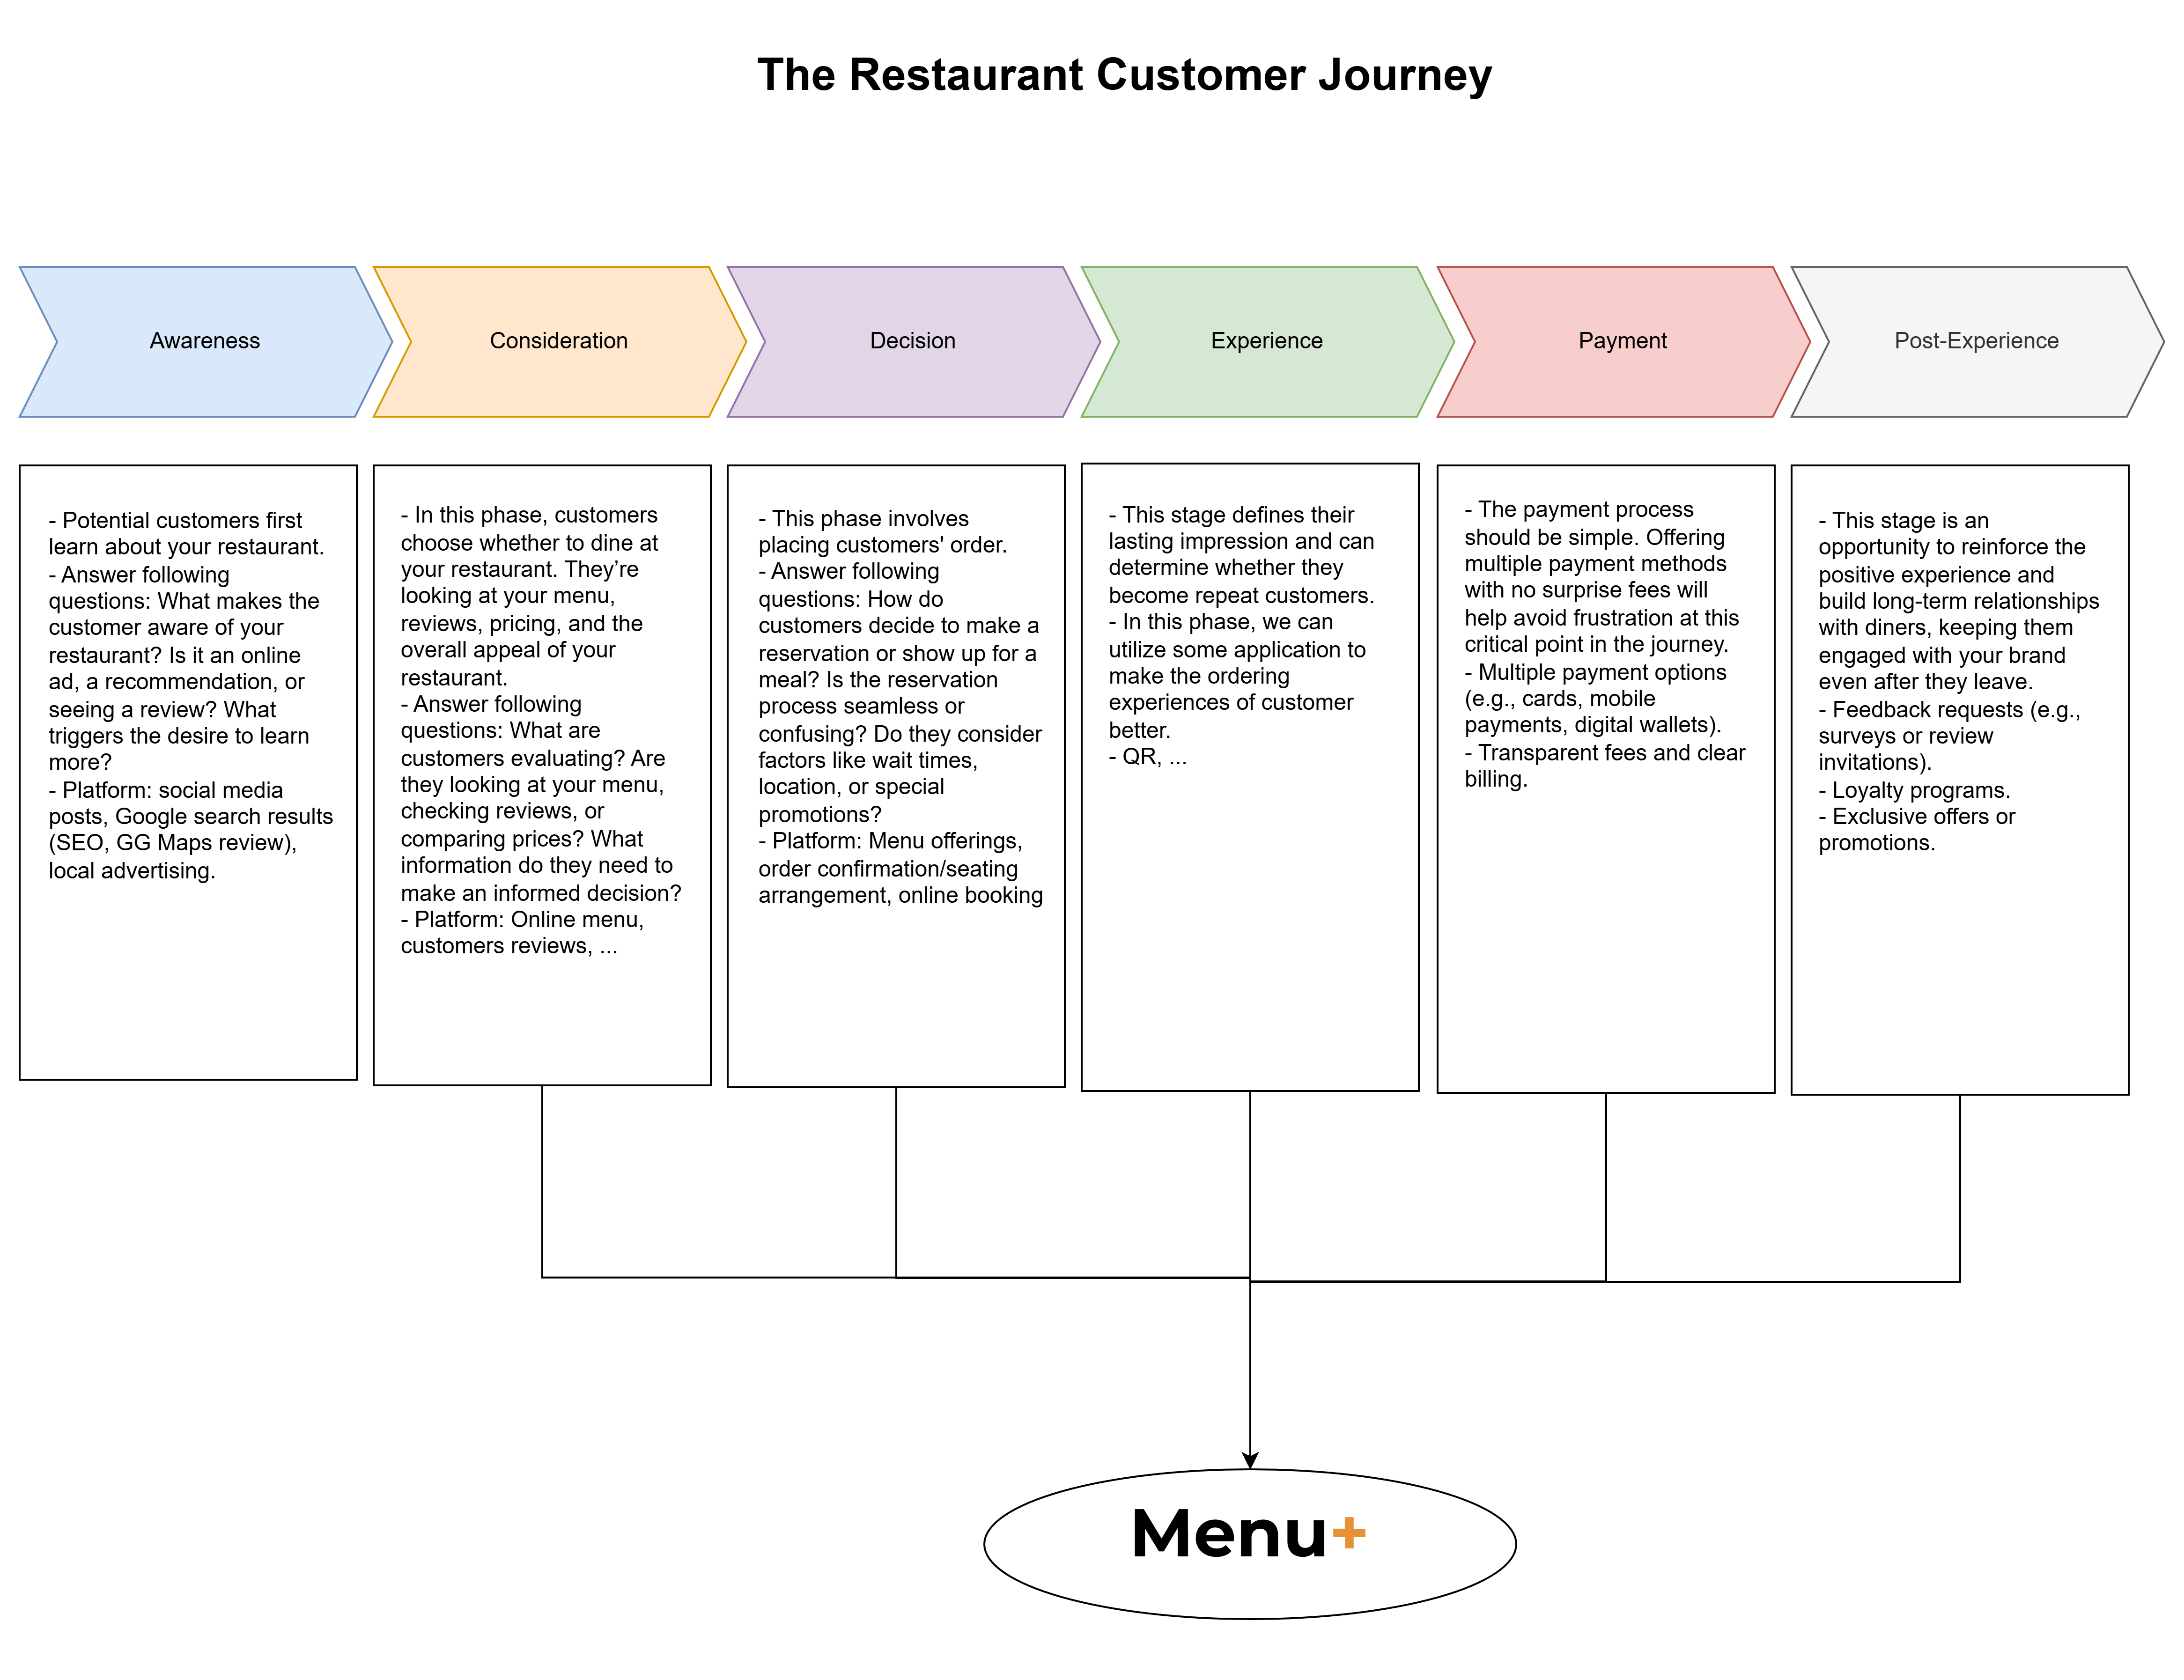
\includegraphics[width=15cm]{Images/restaurant-customer-journey.png}
%     \vspace{0.5cm}
%     \caption{Giới thiệu về Restaunrant Customer Journey}
%     \label{fig:my_label}
% \end{figure}

% % \subsubsection{Lí do chọn mục tiêu "Tích hợp và tối ưu hóa hành trình khách hàng trong dịch vụ nhà hàng"}

% Trong bối cảnh ngành dịch vụ nhà hàng ngày càng cạnh tranh khốc liệt, việc tối ưu hóa hành trình khách hàng không chỉ dừng lại ở việc nâng cao trải nghiệm mà còn trở thành một chiến lược then chốt để cải thiện hiệu quả vận hành và gia tăng lợi thế cạnh tranh. Hệ thống này tập trung vào việc tối ưu hóa các giai đoạn quan trọng trong hành trình khách hàng, bao gồm Cân nhắc, Quyết định, Trải nghiệm, Thanh toán và Hậu trải nghiệm, nhằm mang đến một quy trình đặt món, phục vụ và thanh toán liền mạch, nhanh chóng và thuận tiện. Bên cạnh đó, nhóm cũng hướng đến những mục tiêu song song quan trọng khác, bao gồm:

% \textbf{Đối với Khách hàng:}
% \begin{itemize}
%     \item \textit{Tối ưu trải nghiệm người dùng:}  Cung cấp một giao diện trực quan, thân thiện và dễ sử dụng, cho phép khách hàng dễ dàng khám phá thực đơn, thực hiện đặt món và thanh toán một cách nhanh chóng.
%     \item \textit{Tối ưu hóa trải nghiệm trong các mốc hành tình người dùng:}  Tích hợp các tính năng tiện lợi như quét mã QR để truy cập thực đơn số, đặt món theo thời gian thực và lựa chọn thanh toán linh hoạt, mang đến trải nghiệm nhất quán và không gián đoạn.
%     \item \textit{Minh bạch và tin cậy:}  Đảm bảo tính minh bạch tuyệt đối và rõ ràng trong mọi thông tin, bao gồm giá cả, các chương trình ưu đãi đặc biệt và lịch sử đặt món chi tiết.
% \end{itemize}

% \textbf{Đối với Nhân viên Nhà hàng:}
% \begin{itemize}
%     \item \textit{Nâng cao hiệu suất và độ chính xác:}  Hỗ trợ nhân viên trong việc theo dõi và xử lý các đơn hàng một cách nhanh chóng, chính xác, giảm thiểu sai sót và tăng năng suất.
%     \item \textit{Giảm tải công việc thủ công:}  Tích hợp các công cụ quản lý thông minh để giảm bớt gánh nặng công việc thủ công, từ đó giải phóng thời gian và nguồn lực cho các hoạt động quan trọng khác.
% \end{itemize}

% \textbf{Đối với Nhà Quản lý:}
% \begin{itemize}
%     \item \textit{Cung cấp công cụ hỗ trợ báo cáo và phân tích chi tiết:}  Giúp quản lý dễ dàng theo dõi doanh thu, phân tích xu hướng bán hàng và đánh giá hiệu quả hoạt động tổng thể của nhà hàng.
%     \item \textit{Quản lý hiệu quả nguồn lực:}  Tích hợp chức năng quản lý kho nguyên liệu và nhân sự, hỗ trợ việc ra quyết định nhanh chóng và hiệu quả, tối ưu hóa chi phí và đảm bảo nguồn cung ổn định.
%     \item \textit{Tính linh hoạt cao:}  Đảm bảo khả năng mở rộng và tích hợp dễ dàng các tính năng mới trong tương lai, phù hợp với sự phát triển không ngừng của nhà hàng và sự thay đổi của nhu cầu thị trường.
% \end{itemize}

% \textbf{Về mặt kỹ thuật:}

% \begin{itemize}
%     \item \textit{Hiệu suất và bảo mật tối ưu:}  Thiết kế một hệ thống có hiệu suất cao, khả năng xử lý đồng thời nhiều tác vụ và đảm bảo bảo mật tuyệt đối cho dữ liệu người dùng.
%     \item \textit{Kiến trúc linh hoạt và dễ bảo trì:}  Xây dựng một kiến trúc hệ thống linh hoạt, dễ dàng bảo trì, nâng cấp và mở rộng để đáp ứng nhu cầu phát triển trong tương lai.
% \end{itemize}


% \subsection{Mục tiêu đề tài}

% Mục tiêu của đề tài là xây dựng một hệ thống quản lý đặt món hiện đại, tích hợp các giải pháp công nghệ để tối ưu hóa quy trình vận hành nhà hàng và nâng cao trải nghiệm khách hàng, đồng thời khắc phục các hạn chế của phương pháp quản lý truyền thống đã nêu. Hệ thống này tập trung vào việc tự động hóa các quy trình từ đặt món, quản lý đơn hàng đến thanh toán, đồng thời cung cấp các công cụ phân tích và quản lý hiệu quả cho nhà hàng. Dự án hướng đến việc mang lại lợi ích thiết thực cho khách hàng, nhân viên và quản lý, góp phần thúc đẩy sự phát triển bền vững của ngành công nghiệp nhà hàng trong kỷ nguyên số.

% \begin{enumerate}
%     \item \textbf{Đối với Khách hàng:}
%         \begin{itemize}
%             \item \textit{Tối ưu trải nghiệm người dùng:} Cung cấp giao diện thân thiện, trực quan, cho phép khách hàng dễ dàng truy cập thực đơn, đặt món nhanh chóng và thanh toán linh hoạt qua các phương thức điện tử, như ví điện tử hoặc mã QR, nhằm mang lại trải nghiệm liền mạch.
%             \item \textit{Minh bạch và tin cậy:} Đảm bảo thông tin về giá cả, chương trình ưu đãi và lịch sử đặt món được trình bày rõ ràng, minh bạch, xây dựng niềm tin và sự hài lòng của khách hàng.
%             \item \textit{Cá nhân hóa trải nghiệm:} Sử dụng dữ liệu lịch sử đặt món để cung cấp các ưu đãi và khuyến mãi phù hợp, khuyến khích khách hàng quay lại và tham gia các chương trình khách hàng thân thiết.
%         \end{itemize}

%     \item \textbf{Đối với Nhân viên Nhà hàng:}
%         \begin{itemize}
%             \item \textit{Nâng cao hiệu suất và độ chính xác:} Hỗ trợ nhân viên xử lý đơn hàng nhanh chóng, giảm thiểu sai sót trong quá trình phục vụ, đặc biệt vào giờ cao điểm, thông qua các tính năng tự động hóa.
%             \item \textit{Giảm tải công việc thủ công:} Tích hợp công cụ quản lý thông minh để giảm bớt các tác vụ ghi chép thủ công, giúp nhân viên tập trung vào việc nâng cao chất lượng dịch vụ.
%         \end{itemize}

%     \item \textbf{Đối với Nhà Quản lý:}
%         \begin{itemize}
%             \item \textit{Cung cấp công cụ phân tích và báo cáo:} Hỗ trợ quản lý theo dõi doanh thu, phân tích xu hướng bán hàng và đánh giá hiệu quả hoạt động thông qua các báo cáo chi tiết, từ đó đưa ra quyết định kinh doanh chiến lược.
%             \item \textit{Quản lý hiệu quả nguồn lực:} Tích hợp chức năng quản lý kho, tối ưu hóa lịch làm việc của nhân viên và đảm bảo nguồn cung ổn định, giúp giảm chi phí và nâng cao hiệu quả vận hành.
%         \end{itemize}
% \end{enumerate}

\subsection{Mục tiêu đề tài}

Đề tài hướng đến xây dựng một \textbf{Hệ thống Quản lý Đặt món Hiện đại, Tích hợp và Hiệu quả}, đáp ứng nhu cầu vận hành của nhà hàng trong bối cảnh chuyển đổi số mạnh mẽ của ngành dịch vụ ăn uống. Hệ thống được thiết kế để vượt qua các hạn chế của phương pháp quản lý thủ công, như sai sót trong xử lý đơn hàng, giao tiếp không hiệu quả giữa các bộ phận và trải nghiệm khách hàng chưa tối ưu. Thông qua việc cung cấp giao diện thân thiện, hệ thống cho phép khách hàng dễ dàng xem thực đơn, đặt món, tùy chỉnh yêu cầu, theo dõi trạng thái đơn hàng và thanh toán nhanh chóng bằng nhiều phương thức, từ đó nâng cao sự tiện lợi và hài lòng. Đồng thời, hệ thống tối ưu hóa quy trình làm việc của nhân viên phục vụ, bếp/bar và thu ngân bằng các công cụ quản lý thông minh, giúp giảm thiểu sai sót, tăng tốc độ phục vụ và cung cấp báo cáo doanh thu chi tiết để hỗ trợ quản lý. Qua đó, hệ thống không chỉ hiện đại hóa quy trình vận hành mà còn góp phần giảm chi phí dài hạn, nâng cao hiệu quả quản lý và tạo lợi thế cạnh tranh bền vững cho nhà hàng.

% Trên cơ sở phân tích bối cảnh, động lực và những thách thức đã nêu, đề tài này đặt ra mục tiêu xây dựng một \textbf{Hệ thống Quản lý Đặt món Hiện đại, Tích hợp và Hiệu quả} cho nhà hàng. Hệ thống không chỉ nhằm giải quyết các hạn chế của phương pháp quản lý truyền thống mà còn được thiết kế để \textbf{trực tiếp đối phó và vượt qua các thách thức} đã được xác định, đáp ứng các kỳ vọng ngày càng cao của khách hàng và yêu cầu vận hành trong kỷ nguyên số.

% Các mục tiêu cụ thể của hệ thống, tập trung vào các tính năng chính và cách chúng giải quyết thách thức, bao gồm:

% \begin{enumerate}
%     \item \textbf{Đối với Khách hàng:} Nâng cao trải nghiệm đặt món và thanh toán, mang lại sự tiện lợi và chủ động.
%         \begin{itemize}
%             \item \textit{Xem thực đơn điện tử:} Truy cập thực đơn trực quan (hình ảnh, mô tả, giá cả) dễ dàng qua thiết bị di động hoặc kiosk tại bàn.
%             \item \textit{Đặt món và tùy chỉnh:} Chọn món, điều chỉnh số lượng, và dễ dàng thêm các yêu cầu đặc biệt (ví dụ: ít cay, không hành, thêm phô mai).
%             \item \textit{Theo dõi trạng thái đơn hàng:} Có thể xem được trạng thái đơn hàng của mình (đang chờ xác nhận, đang chuẩn bị, đã sẵn sàng - tùy mức độ triển khai).
%             \item \textit{Yêu cầu thanh toán và thanh toán tiện lợi:} Gọi thanh toán và thực hiện thanh toán nhanh chóng qua các phương thức đa dạng như tiền mặt, thẻ, và đặc biệt là quét mã QR ngay tại bàn (\textit{giải quyết phần nào thách thức về tích hợp thanh toán điện tử}).
%             \item \textit{Gọi phục vụ:} Có chức năng gọi nhân viên hỗ trợ khi cần thiết thông qua hệ thống.
%         \end{itemize}

%     \item \textbf{Đối với Nhân viên Phục vụ:} Tối ưu hóa quy trình nhận và chuyển đơn hàng, giảm sai sót và tăng tốc độ phục vụ.
%         \begin{itemize}
%             \item \textit{Ghi nhận đơn hàng di động:} Sử dụng máy tính bảng hoặc thiết bị POS di động để nhận đơn ngay tại bàn, giảm thiểu việc ghi chép thủ công.
%             \item \textit{Gửi đơn hàng tự động:} Đơn hàng được gửi tức thì và chính xác đến bộ phận bếp và/hoặc bar thông qua màn hình hiển thị.
%             \item \textit{Quản lý trạng thái bàn:} Dễ dàng theo dõi trạng thái các bàn (trống, đang có khách, đã đặt trước, cần dọn dẹp).
%             \item \textit{Xử lý yêu cầu đặc biệt:} Ghi chú và chuyển các yêu cầu đặc biệt của khách hàng một cách rõ ràng.
%             \item \textit{Hỗ trợ thanh toán tại bàn:} Thực hiện quy trình thanh toán (in hóa đơn tạm, xác nhận thanh toán) hiệu quả hơn.
%         \end{itemize}

%     \item \textbf{Đối với Nhân viên Bếp/Bar:} Nhận thông tin đơn hàng chính xác và kịp thời, tối ưu hóa quy trình chế biến.
%         \begin{itemize}
%             \item \textit{Hiển thị đơn hàng điện tử (Kitchen Display System - KDS):} Nhận đơn hàng rõ ràng trên màn hình, bao gồm chi tiết món và các tùy chỉnh, thay vì phiếu giấy dễ thất lạc hoặc nhòe mực.
%             \item \textit{Quản lý thứ tự chế biến:} Hệ thống có thể hỗ trợ sắp xếp thứ tự ưu tiên của các đơn hàng hoặc món ăn.
%             \item \textit{Đánh dấu trạng thái món ăn:} Thông báo cho bộ phận phục vụ khi món ăn đã sẵn sàng để phục vụ.
%         \end{itemize}

%     \item \textbf{Đối với Nhân viên Thu ngân và Quản lý:} Cung cấp công cụ quản lý hiệu quả, theo dõi doanh thu và hiệu suất hoạt động.
%         \begin{itemize}
%             \item \textit{Quản lý hóa đơn và thanh toán tập trung:} Dễ dàng xem lại, in ấn, và xử lý thanh toán cho các hóa đơn.
%             \item \textit{Áp dụng khuyến mãi, giảm giá:} Hệ thống hỗ trợ việc thiết lập và áp dụng các chương trình khuyến mãi một cách linh hoạt.
%             \item \textit{Báo cáo doanh thu chi tiết:} Cung cấp các báo cáo doanh thu theo thời gian (ngày, tuần, tháng), theo món ăn, theo nhân viên, giúp quản lý nắm bắt tình hình kinh doanh.
%             \item \textit{Quản lý thực đơn và giá bán:} Cho phép quản lý dễ dàng cập nhật thực đơn, giá cả và mô tả món ăn.
%             \item \textit{Quản lý tài khoản người dùng:} Phân quyền truy cập và sử dụng hệ thống cho từng vai trò nhân viên.
%         \end{itemize}

%     \item \textbf{Mục tiêu Hệ thống Tổng thể - Trực tiếp giải quyết các thách thức cốt lõi:}
%         \begin{itemize}
%             \item \textit{Tính ổn định và hiệu năng:} Đảm bảo hệ thống hoạt động mượt mà, ổn định, đặc biệt trong các giờ cao điểm, giảm thiểu tối đa thời gian chết (\textit{giải quyết thách thức về quản lý lỗi và vận hành liên tục}).
%             \item \textit{Tính bảo mật cao:} Xây dựng các cơ chế bảo mật mạnh mẽ để bảo vệ dữ liệu giao dịch, thông tin khách hàng và dữ liệu kinh doanh, tuân thủ các quy định pháp luật (\textit{giải quyết thách thức về bảo mật dữ liệu và quyền riêng tư}).
%             \item \textit{Kiến trúc linh hoạt và khả năng tích hợp:} Thiết kế hệ thống theo kiến trúc module, sử dụng các API rõ ràng để dễ dàng tích hợp với các thiết bị phần cứng phổ biến (máy in, máy POS) và có thể mở rộng để tích hợp với các hệ thống khác (kế toán, kho) trong tương lai (\textit{giải quyết thách thức về độ phức tạp kỹ thuật và tích hợp hệ thống}).
%             \item \textit{Giao diện thân thiện và trực quan (UX/UI):} Ưu tiên thiết kế giao diện người dùng đơn giản, dễ học, dễ sử dụng cho tất cả các đối tượng, từ khách hàng đến nhân viên và quản lý, nhằm giảm thời gian đào tạo và tăng tỷ lệ chấp nhận (\textit{giải quyết thách thức về thiết kế trải nghiệm người dùng và đào tạo/thay đổi thói quen}).
%             \item \textit{Quản lý dữ liệu hiệu quả:} Thiết kế cơ sở dữ liệu tối ưu để xử lý khối lượng lớn giao dịch và thông tin, đảm bảo khả năng truy vấn và báo cáo nhanh chóng (\textit{giải quyết thách thức về quản lý dữ liệu lớn}).
%             % Lưu ý: Thách thức về chi phí, thời gian và nhân lực được giải quyết thông qua việc lập kế hoạch dự án, lựa chọn công nghệ phù hợp và quản lý hiệu quả, hơn là một tính năng trực tiếp của hệ thống. Tuy nhiên, một hệ thống hiệu quả, dễ sử dụng và bảo trì sẽ góp phần giảm chi phí vận hành và đào tạo dài hạn.
%         \end{itemize}
% \end{enumerate}

% Việc đạt được các mục tiêu này không chỉ mang lại các tính năng mong đợi mà còn trực tiếp tháo gỡ những rào cản và khó khăn đã được nhận diện. Qua đó, hệ thống sẽ góp phần hiện đại hóa quy trình vận hành, nâng cao sự hài lòng của khách hàng, tăng cường hiệu quả quản lý và tạo lợi thế cạnh tranh bền vững cho nhà hàng trong bối cảnh ngành F\&B đang chuyển đổi số mạnh mẽ.

\subsection{Phạm vi đề tài}

Để đảm bảo dự án khả thi và tập trung vào việc giải quyết các mục tiêu cốt lõi trong khung thời gian và nguồn lực hạn chế, phạm vi của đề tài được xác định rõ ràng như sau:

\subsubsection{Phạm vi Chức năng}

Hệ thống sẽ tập trung vào các chức năng thiết yếu cho quy trình đặt món và quản lý cơ bản tại một nhà hàng điển hình. Các chức năng chính bao gồm:
        \begin{itemize}
            \item Quản lý Thực đơn: Thêm, sửa, xóa, ẩn/hiện món ăn, danh mục món ăn, quản lý giá bán và mô tả cơ bản.
            \item Quản lý Bàn/Khu vực: Thiết lập sơ đồ bàn, quản lý trạng thái bàn (trống, đang phục vụ, đã đặt, cần dọn).
            \item Quy trình Đặt món tại bàn: Nhân viên phục vụ nhận đơn qua thiết bị di động (máy tính bảng/điện thoại), gửi đơn tự động đến bếp/bar. Bao gồm khả năng chọn món, tùy chỉnh số lượng, ghi chú đơn giản.
            \item Hiển thị Đơn hàng tại Bếp (Kitchen Display System - KDS): Hiển thị danh sách các món cần chế biến, trạng thái món, ... lên màn hình.
            \item Quản lý Đơn hàng cơ bản: Xem danh sách đơn hàng, trạng thái đơn hàng.
            \item Quy trình Thanh toán: Hỗ trợ tạo hóa đơn tạm, áp dụng giảm giá đơn giản (theo phần trăm hoặc số tiền cố định), ghi nhận thanh toán bằng tiền mặt và tích hợp thanh toán cơ bản qua ví điện tử.
            \item Báo cáo cơ bản: Báo cáo doanh thu theo ngày, báo cáo các món bán chạy trong ngày.
            \item Quản lý Tài khoản người dùng: Tạo và quản lý tài khoản cho các vai trò (Quản lý, Phục vụ, Bếp, Thu ngân, Quản lý) với phân quyền truy cập chức năng tương ứng.
        \end{itemize}

\subsubsection{Phạm vi Kỹ thuật}

Các giới hạn và lựa chọn về mặt công nghệ được xác định như sau:

\begin{itemize}
    \item \textbf{Kiến trúc hệ thống:} Dự kiến xây dựng theo kiến trúc ứng dụng kiến trúc Client-Server cơ bản để đơn giản hóa việc phát triển và triển khai trong giai đoạn đầu.
    \item \textbf{Công nghệ phát triển (Dự kiến):}
        \begin{itemize}
            \item \textit{Frontend (Giao diện người dùng):} Sử dụng một framework JavaScript hiện đại như React cùng với ShadcnUI và TailwindCSS để xây dựng giao diện tương tác và responsive.
            \item \textit{Backend (Xử lý logic):} Sử dụng một nền tảng phía máy chủ phổ biến Java (với Spring Boot) dựa trên kinh nghiệm của thành viên trong nhóm và các đặc điểm của nền tảng.
            \item \textit{Cơ sở dữ liệu:} Sử dụng hệ quản trị cơ sở dữ liệu quan hệ (SQL) PostgreSQL để đảm bảo tính nhất quán dữ liệu.
            \item \textit{Giao tiếp Real-time (nếu cần cho KDS/cập nhật trạng thái):} Có thể sử dụng WebSockets hoặc các kỹ thuật tương tự.
        \end{itemize}
    \item \textbf{Nền tảng triển khai:} Hệ thống chủ yếu hoạt động trên trình duyệt Web trên các thiết bị như máy tính, máy POS, máy tính bảng. Chưa bao gồm việc phát triển ứng dụng di động gốc (Native Mobile App) cho iOS hay Android trong phạm vi này.
    \item \textbf{Bảo mật:} Áp dụng các biện pháp bảo mật cơ bản như mã hóa mật khẩu, bảo vệ chống lại các lỗ hổng web phổ biến, phân quyền dựa trên vai trò. Không bao gồm các biện pháp kiểm thử xâm nhập (penetration testing) chuyên sâu.
\end{itemize}
\subsection{Cấu trúc báo cáo đồ án}
Cấu trúc bài báo cáo bao gồm 7 chương:
\begin{itemize}
    \item \textbf{Chương 1 - Giới thiệu}: Trình bày bối cảnh, động lực, thách thức, mục tiêu và phạm vi của đề tài.
    \item \textbf{Chương 2 - Cơ sở lý thuyết}: Cung cấp nền tảng lý thuyết về lĩnh vực nhà hàng và công nghệ.
    \item \textbf{Chương 3 - Các hệ thống liên quan}: So sánh các hệ thống quản lý hiện có và rút ra bài học.
    \item \textbf{Chương 4 - Tổng quan hệ thống}: Mô tả bối cảnh, yêu cầu và quy trình tổng quát của hệ thống.
    \item \textbf{Chương 5 - Thiết kế}: Thiết kế Sitemap, giao diện, cơ sở dữ liệu, API và kiến trúc triển khai.
    \item \textbf{Chương 6 - Tổng kết}: Tóm tắt những gì đã thực hiện trong giai đoạn thiết kế, đồng thời định hướng phát triển và triển khai trong giai đoạn tiếp theo.
    \item \textbf{Chương 7 - Kế hoạch phát triển}: Liệt kê chi tiết các đầu việc, tính năng và kiểm thử dự kiến sẽ thực hiện trong giai đoạn phát triển hệ thống.
\end{itemize}


% \newpage
% \section{CƠ SỞ LÝ THUYẾT}
\subsection{Tìm hiểu về Restaurant Industry}

\subsubsection{Nhà hàng ăn uống cao cấp (Fine dining restaurant)}
\subsubsubsection{Tổng quan}
Fine dining được định nghĩa là trải nghiệm nhà hàng tinh tế, thường đắt đỏ và đặc biệt hơn so với nhà hàng thông thường. Đặc điểm bao gồm sử dụng khăn trải bàn trắng, dịch vụ bàn bởi nhân viên được đào tạo, và không gian sang trọng với vật liệu cao cấp. Lịch sử cho thấy fine dining bắt đầu vào những năm 1780 tại Paris, với các nhà hàng như Trois Frères và La Grande Taverne de Londres, và sau đó lan sang Hoa Kỳ với Delmonico's ở New York, nổi tiếng với hầm rượu 1.000 chai. Trong thời kì hiện đại, fine dining tập trung vào sự sáng tạo và dịch vụ hoàn hảo.\\


\begin{figure}[H]
	\centering
	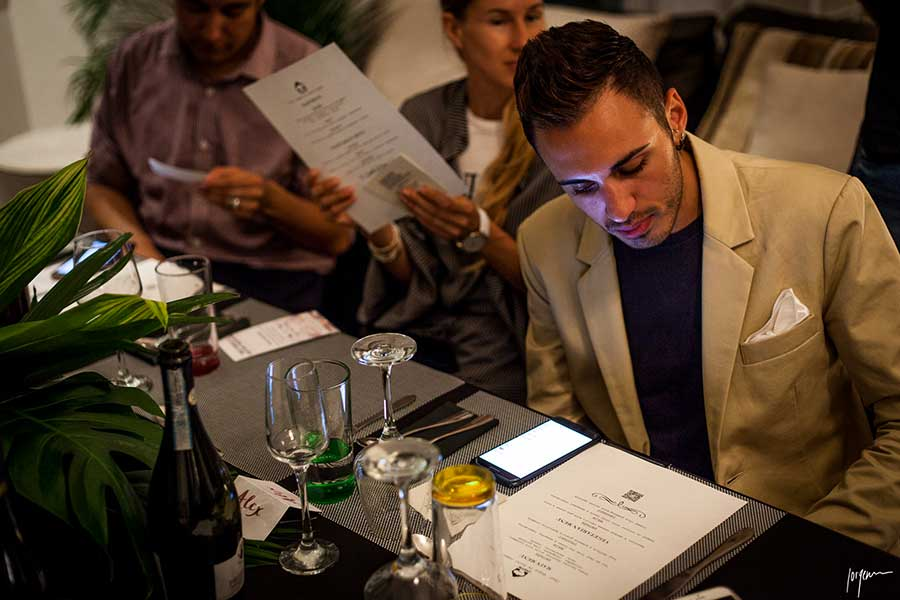
\includegraphics[width=15cm]{Images/fine-dining.jpg}
	\vspace{0.5cm}
	\caption{Nhà hàng fine dining. Nguồn: \href{https://chefin.com/blog/the-past-and-future-of-fine-dining/}{chefin.com}}
	\label{fig:my_label}
\end{figure}

Nhà hàng fine dining hoạt động dựa trên mô hình kinh doanh cân bằng giữa chi phí vận hành cao và giá bán cao cấp. Chi phí bao gồm nguyên liệu cao cấp, lao động có kỹ năng, và sự chú ý chi tiết trong cả chuẩn bị món ăn và dịch vụ. Doanh thu chủ yếu đến từ việc bán bữa ăn, với giá cao hơn nhiều so với nhà hàng ăn uống thông thường, phản ánh chất lượng và sự độc quyền của trải nghiệm. Ngoài ra, các chương trình rượu vang và đồ uống cũng đóng góp đáng kể vào doanh thu, cùng với các dịch vụ như tiệc riêng, catering, và bán hàng hóa. \\

Tuy nhiên, lợi nhuận trong fine dining là một thách thức do chi phí cố định và biến đổi cao. Chi phí cố định bao gồm tiền thuê ở vị trí đắc địa, trang trí cao cấp, và thiết bị, trong khi chi phí biến đổi bao gồm nguyên liệu đắt tiền và lao động cho đội ngũ được đào tạo bài bản. Thành công phụ thuộc vào việc duy trì tỷ lệ khách cao, khách hàng trung thành, và danh tiếng mạnh, có thể dẫn đến các giải thưởng như sao Michelin, từ đó thúc đẩy nhu cầu. \\

Fine dining hiện đại đã phát triển, nhấn mạnh vào sự sáng tạo và dịch vụ hoàn hảo. Sự kết hợp giữa chỗ ở sang trọng và ẩm thực cao cấp, như được tiên phong bởi César Ritz và Auguste Escoffier tại Grand Hotel of Monte Carlo, đã nâng tầm vị thế của fine dining.


\subsubsubsection{Sơ đồ tổ chức (Organization chart)}
Trong ngành công nghiệp nhà hàng, đặc biệt là nhà hàng ẩm thực cao cấp, sơ đồ tổ chức đóng vai trò quan trọng trong việc định hình cấu trúc, đảm bảo bộ máy hoạt động hiệu quả. Biểu đồ tổ chức giúp làm rõ mối quan hệ giữa các vị trí công việc, xác định ai báo cáo cho ai, và ai chịu trách nhiệm cho những nhiệm vụ cụ thể nào. Điều này đặc biệt quan trọng trong nhà hàng ẩm thực cao cấp, nơi mà chất lượng dịch vụ và sự hài lòng của khách hàng là yếu tố hàng đầu. \\
Nhà hàng ẩm thực cao cấp thường có cấu trúc tổ chức phức tạp và đa tầng, phản ánh nhu cầu cung cấp dịch vụ cá nhân hóa và sang trọng:

\begin{itemize}
	\item Quản trị viên: Vai trò này đảm bảo rằng nhà hàng tuân thủ các quy định pháp lý và hoạt động hành chính suôn sẻ. Họ xử lý thuế, làm việc với nhà cung cấp, và quản lý các vấn đề tài chính, tạo nền tảng cho hoạt động của nhà hàng.
	\item Quản lý: Là người giám sát tổng thể, đảm bảo rằng mọi bộ phận hoạt động hài hòa. Họ làm cầu nối giữa quản trị viên và các trưởng bộ phận, đảm bảo dịch vụ đạt tiêu chuẩn cao cấp.
	\item Quản lý nhà bếp: Vai trò này tập trung vào việc duy trì nguồn cung nguyên liệu chất lượng, làm việc chặt chẽ với đầu bếp trưởng để đảm bảo nhà bếp hoạt động hiệu quả.
	\item Đầu bếp trưởng: Là linh hồn của nhà hàng, chịu trách nhiệm cho tầm nhìn ẩm thực. Họ tạo ra thực đơn sáng tạo, phản ánh phong cách của nhà hàng, và giám sát toàn bộ hoạt động nhà bếp để đảm bảo chất lượng và sự nhất quán.
	\item Phó đầu bếp: Hỗ trợ đầu bếp trưởng, đảm bảo rằng mọi món ăn được chuẩn bị và trình bày đúng tiêu chuẩn, đặc biệt trong giờ cao điểm.
	\item Đầu bếp chuyên khoa: Mỗi station chef chịu trách nhiệm cho một lĩnh vực cụ thể, như món khai vị hoặc món chính, đảm bảo chuyên môn hóa và chất lượng cao.
	\item Đầu bếp, trợ lý: Là lực lượng hỗ trợ chính, thực hiện các nhiệm vụ hàng ngày như chuẩn bị nguyên liệu và nấu nướng, đảm bảo nhà bếp hoạt động trơn tru.
	\item Người rửa chén, nhân viên dọn dẹp hậu trường: Vai trò này rất quan trọng để duy trì vệ sinh, đảm bảo an toàn thực phẩm, và giữ cho nhà bếp luôn sẵn sàng.
	\item Trưởng phục vụ (Maitre d'): Là gương mặt đại diện của nhà hàng, đảm bảo khách hàng có trải nghiệm đầu tiên ấn tượng. Họ quản lý danh sách đặt chỗ và hướng dẫn khách, tạo nên bầu không khí chuyên nghiệp.
	\item Nhân viên phục vụ: Đảm bảo khách hàng được phục vụ chu đáo, từ việc lấy order đến phục vụ món ăn, góp phần vào trải nghiệm tổng thể.
	\item Chuyên viên rượu: Là chuyên gia về rượu, họ tư vấn cho khách hàng về các lựa chọn rượu phù hợp, nâng cao trải nghiệm ẩm thực, đặc biệt trong môi trường cao cấp.
	\item Nhân viên dọn dẹp tiền sảnh: Giữ khu vực ăn uống sạch sẽ và ngăn nắp, đảm bảo không gian sang trọng và thoải mái cho khách hàng.
	\item Trưởng bảo vệ: Quản lý an ninh, đảm bảo an toàn cho khách và tài sản, một vai trò quan trọng trong môi trường cao cấp.
	\item Bảo vệ, người đỗ xe: Cung cấp dịch vụ an ninh và đỗ xe, tạo ấn tượng chuyên nghiệp và sang trọng, đặc biệt cho khách hàng sử dụng dịch vụ đỗ xe.
\end{itemize}

\begin{longtable}{| p{4cm} | p{8cm} | p{3cm} |}
	\caption{Vị trí, chức năng và người quản lý trong một nhà hàng ăn uống cao cấp}                                                                                                                                                                               \\
	\hline
	\textbf{Vị trí}                                                                   & \textbf{Chức năng}                                                                                                                              & \textbf{Báo cáo cho}    \\
	\hline
	\endfirsthead

	\hline
	\textbf{Vị trí}                                                                   & \textbf{Chức năng}                                                                                                                              & \textbf{Báo cáo cho}    \\
	\hline
	\endhead

	\hline
	\multicolumn{3}{|c|}{\textit{Còn tiếp}}                                                                                                                                                                                                                       \\
	\hline
	\endfoot

	\hline
	\endlastfoot

	Quản trị viên (Administrator)                                                     & Xử lý thuế, nhà cung cấp, và các nhu cầu hành chính khác. Đảm bảo tuân thủ pháp lý và hoạt động hành chính suôn sẻ.                             & Không có (cấp cao nhất) \\
	\hline
	Quản lý (Manager)                                                                 & Giám sát toàn bộ hoạt động của nhà hàng, bao gồm cả phần front-of-house và back-of-house. Đảm bảo dịch vụ chuyên nghiệp và khách hàng hài lòng. & Quản trị viên           \\
	\hline
	Quản lý nhà bếp (Kitchen Manager)                                                 & Quản lý hàng tồn kho và mua sắm cho nhà bếp, đảm bảo nguyên liệu chất lượng cao. Làm việc chặt chẽ với đầu bếp trưởng.                          & Quản trị viên           \\
	\hline
	Đầu bếp trưởng (Executive Chef)                                                   & Là người lãnh đạo culinaire, tạo thực đơn sáng tạo, giám sát hoạt động nhà bếp, đảm bảo chất lượng và sự nhất quán.                             & Quản lý nhà bếp         \\
	\hline
	Phó đầu bếp (Sous-Chef)                                                           & Hỗ trợ đầu bếp trưởng, giám sát việc chuẩn bị và trình bày món ăn, đảm bảo tiêu chuẩn.                                                          & Đầu bếp trưởng          \\
	\hline
	Đầu bếp chuyên khoa (Station Chef)                                                & Chuyên trách một lĩnh vực cụ thể (khai vị, món chính, tráng miệng), xử lý chuẩn bị phức tạp, giám sát đầu bếp và trợ lý.                        & Phó đầu bếp             \\
	\hline
	Đầu bếp, trợ lý (Cooks, Assistants)                                               & Thực hiện nhiệm vụ được giao, bao gồm chuẩn bị nguyên liệu, nấu nướng, và trình bày món ăn.                                                     & Đầu bếp chuyên khoa     \\
	\hline
	Người rửa chén, nhân viên dọn dẹp hậu trường (Dishwasher, Back of House Cleaners) & Giữ nhà bếp và thiết bị sạch sẽ, đảm bảo vệ sinh và an toàn thực phẩm.                                                                          & Quản lý nhà bếp         \\
	\hline
	Trưởng phục vụ (Maitre d')                                                        & Là gương mặt đầu tiên, hướng dẫn khách, quản lý danh sách đặt chỗ, đảm bảo dịch vụ xuất sắc.                                                    & Quản lý                 \\
	\hline
	Nhân viên phục vụ (Waiters)                                                       & Phục vụ khách, lấy order, phục vụ thức ăn và đồ uống, đảm bảo khách hài lòng.                                                                   & Trưởng phục vụ          \\
	\hline
	Chuyên viên rượu (Sommelier)                                                      & Là chuyên gia về rượu, tư vấn lựa chọn rượu phù hợp, nâng cao trải nghiệm ẩm thực.                                                              & Trưởng phục vụ          \\
	\hline
	Nhân viên dọn dẹp tiền sảnh (Front-of-House Cleaning Staff)                       & Giữ khu vực ăn uống sạch sẽ và ngăn nắp, đảm bảo không gian thoải mái và sang trọng.                                                            & Trưởng phục vụ          \\
	\hline
	Trưởng bảo vệ (Head of Security)                                                  & Quản lý an ninh, giám sát camera, bảo vệ, và người đỗ xe, đảm bảo an toàn cho khách và tài sản.                                                 & Quản lý                 \\
	\hline
	Bảo vệ, người đỗ xe (Guards, Valets)                                              & Cung cấp dịch vụ an ninh và đỗ xe, tạo ấn tượng chuyên nghiệp và sang trọng.                                                                    & Trưởng bảo vệ           \\
	\hline
\end{longtable}


% \clearpage

\begin{figure}[H]
	\centering
	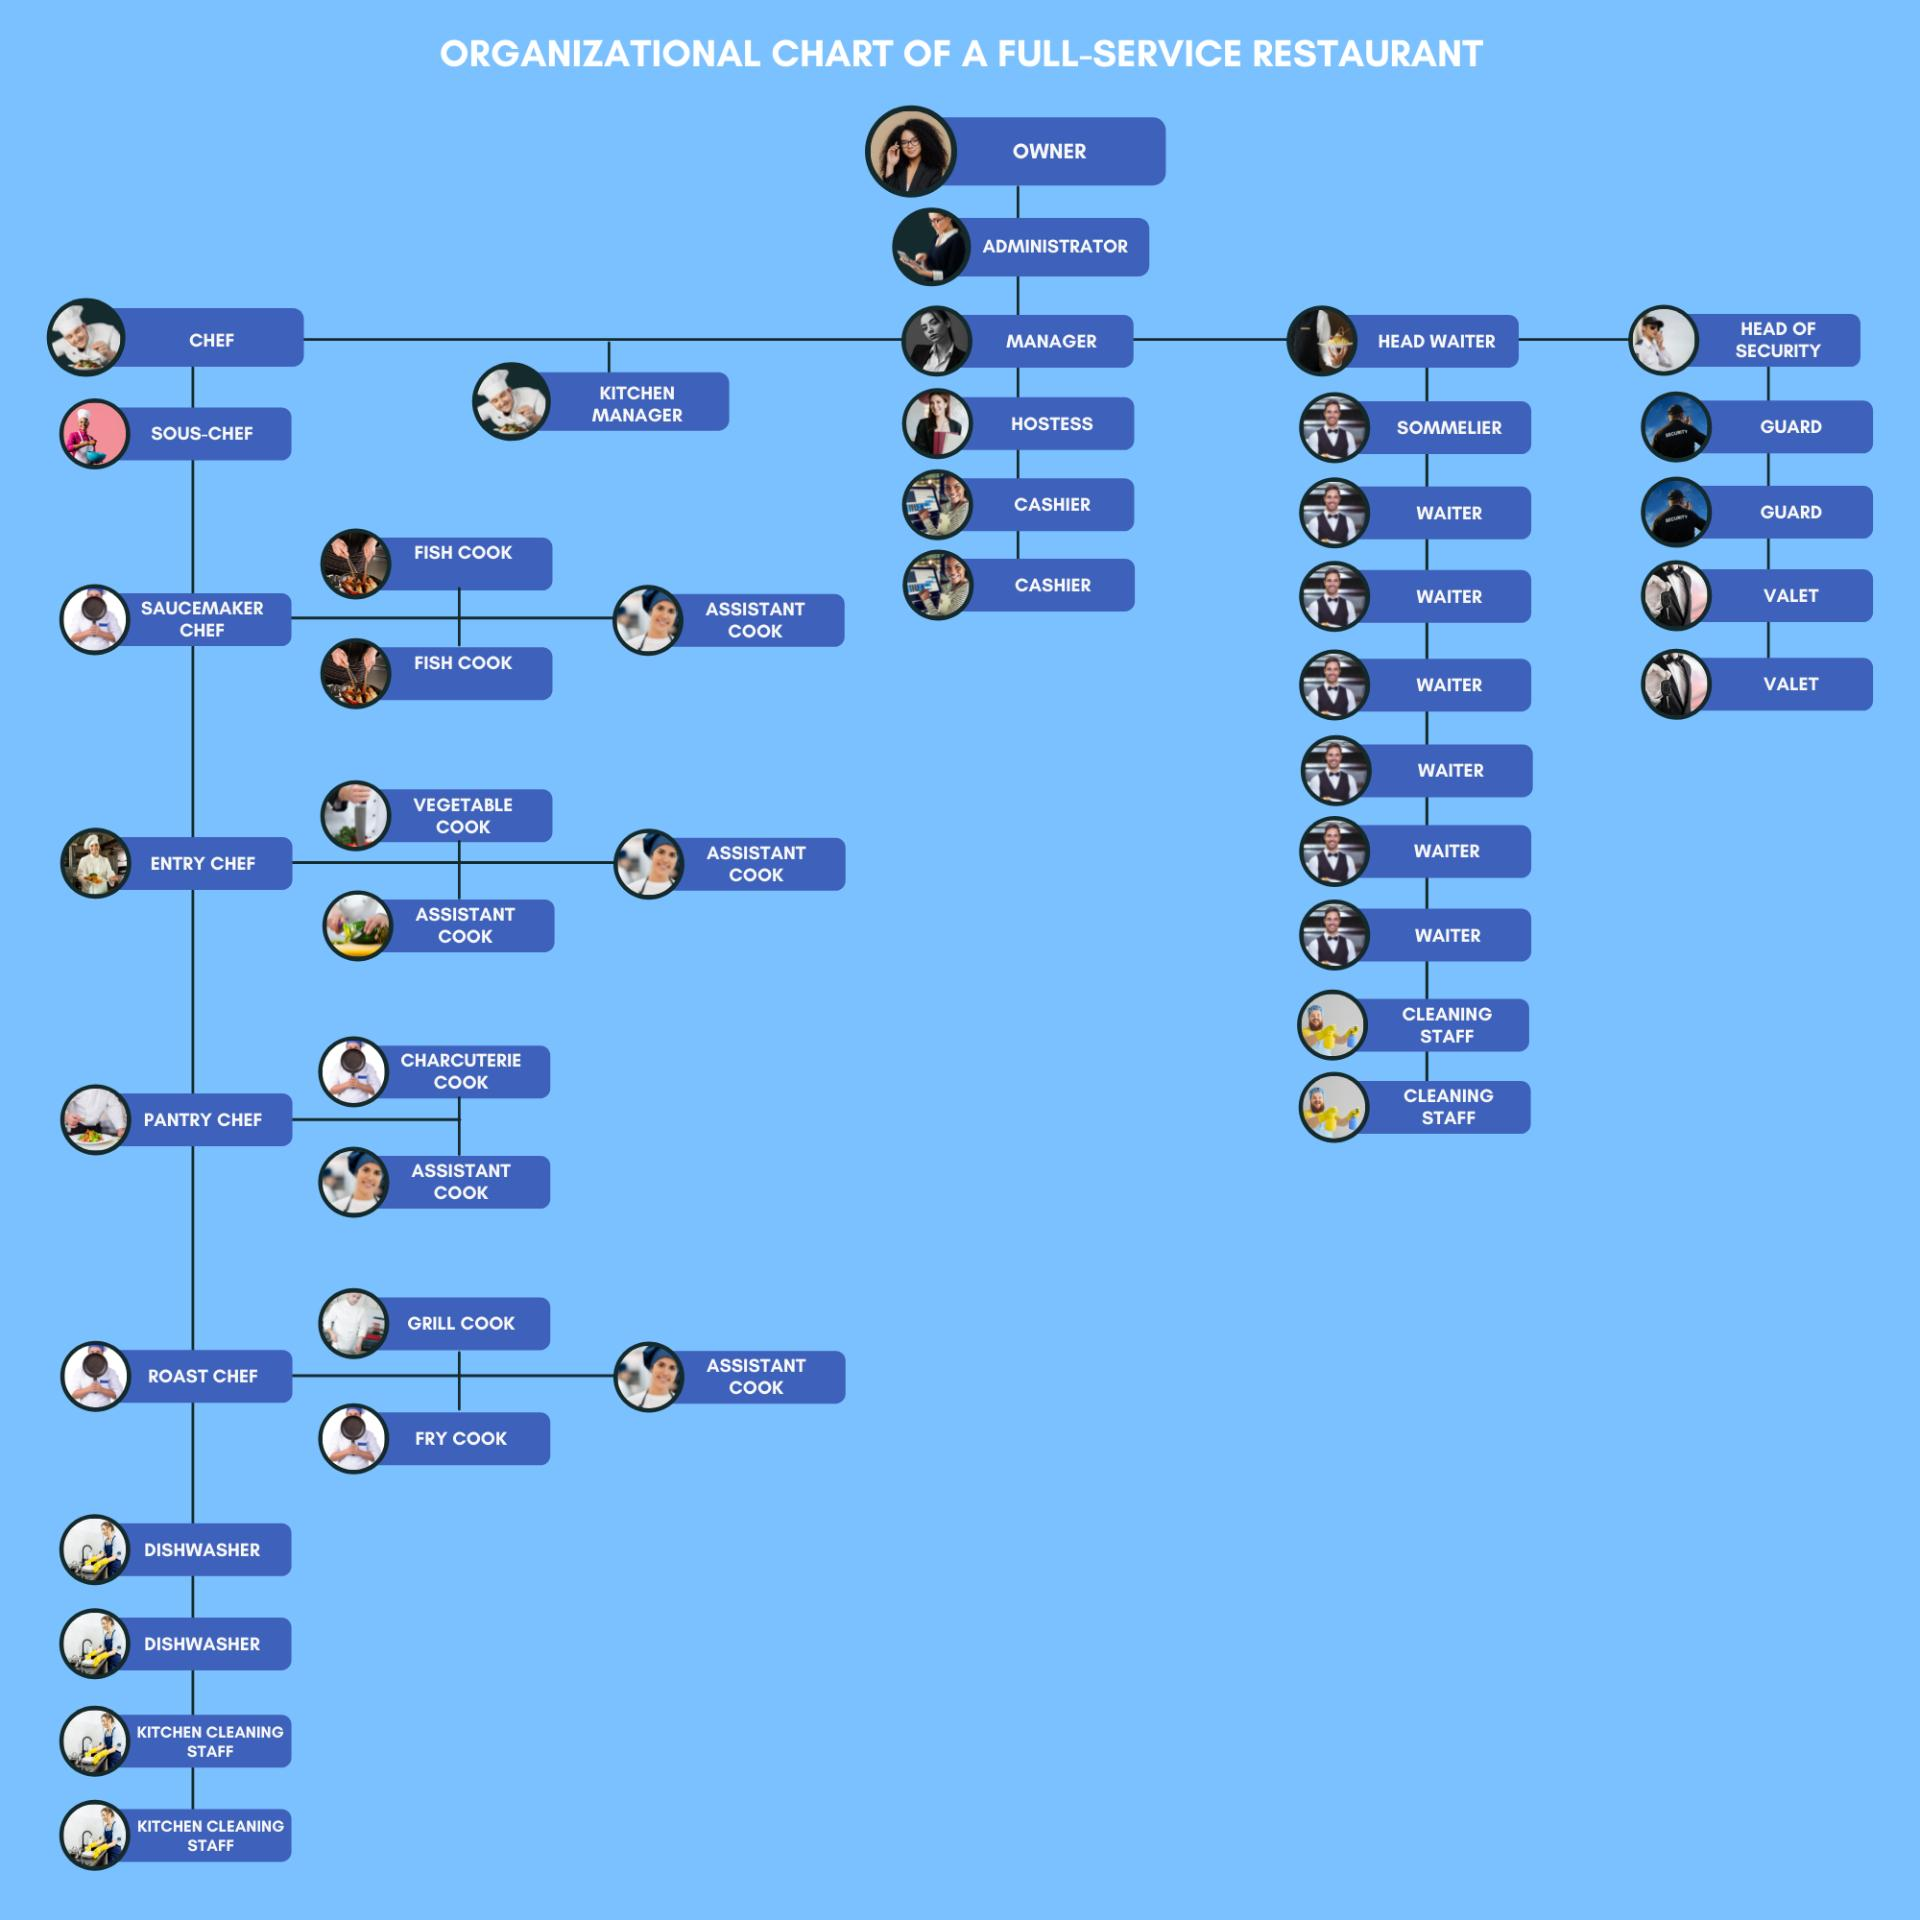
\includegraphics[width=15cm]{Images/finedining_orig_chart.jpg}
	\vspace{0.5cm}
	\caption{Sơ đồ tổ chức cho nhà hàng ăn uống cao cấp. Nguồn: waiterio.com}
\end{figure}

\subsubsection{Nhà hàng ăn uống phục vụ đồ ăn nhanh (Fast-food restaurant)}
\subsubsubsection{Tổng quan}
Nhà hàng thức ăn nhanh, còn được gọi là nhà hàng dịch vụ nhanh (QSR), là cơ sở cung cấp thức ăn được chuẩn bị và phục vụ nhanh chóng, thường trong vòng vài phút, với thực đơn hạn chế như bánh burger, khoai tây chiên, pizza và gà rán, phục vụ trong đồ dùng một lần. Khách hàng thường đặt hàng tại quầy hoặc qua cửa sổ giao hàng, và thức ăn được dự định để ăn tại chỗ hoặc mang đi. \\


\begin{figure}[H]
	\centering
	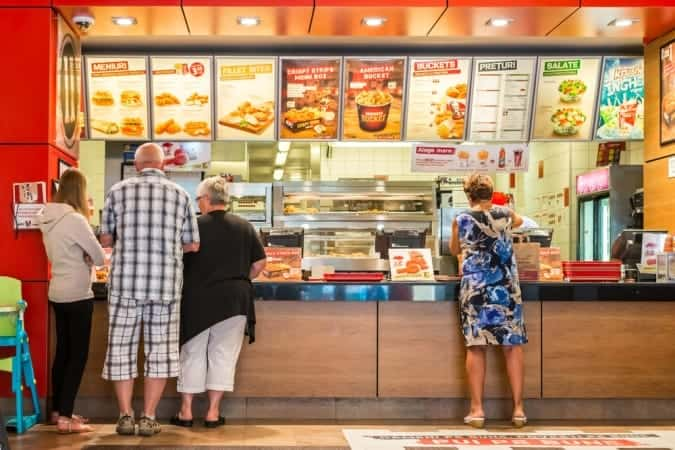
\includegraphics[width=15cm]{Images/fastfood.jpg}
	\vspace{0.5cm}
	\caption{Nhà hàng phụ vụ thức ăn nhanh. Nguồn: \href{https://foodtank.com/news/2015/08/world-health-organization-study-proves-need-for-regulation-of-fast-food/}{foodtank.com}}
\end{figure}

Mô hình kinh doanh của nhà hàng thức ăn nhanh tập trung vào khối lượng lớn và biên lợi nhuận thấp, với thực đơn chuẩn hóa và hệ thống franchise để đảm bảo sự đồng nhất và khả năng mở rộng. Họ nhắm đến thị trường bận rộn, sử dụng tiếp thị mạnh mẽ và nền tảng kỹ thuật số để tiếp cận khách hàng.

Nhà hàng thức ăn nhanh vận hành với các quy trình tinh giản sử dụng bếp dây chuyền để đảm bảo hiệu quả, với chuỗi cung ứng tập trung và công nghệ như hệ thống POS để tối ưu hóa hoạt động. Đào tạo nhân viên tập trung vào tốc độ và chính xác, với mô hình tự phục vụ giảm chi phí lao động.

\subsubsubsection{Sơ đồ tổ chức (Organization chart)}
Nhà hàng thức ăn nhanh thường có cấu trúc tổ chức đơn giản và phẳng, phản ánh nhu cầu cung cấp dịch vụ nhanh chóng và hiệu quả:
\begin{itemize}
	\item Quản lý điều hành: Giám sát toàn bộ hoạt động, bao gồm tuyển dụng và ngân sách.
	\item Quản lý ca: Giám sát nhân viên trong ca, xử lý khiếu nại khách hàng.
	\item Nhân viên thu ngân: Xử lý thanh toán và đơn hàng.
	\item Đầu bếp: Chuẩn bị thức ăn, đảm bảo chất lượng.
	\item Nhân viên vệ sinh: Giữ nhà hàng sạch sẽ, đặc biệt quan trọng trong môi trường cao áp lực.
\end{itemize}
\begin{table}[ht]
	\centering
	\caption{Vị trí, chức năng và người quản lý trong một nhà hàng phục vụ đồ ăn nhanh}
	\resizebox{\textwidth}{!}{
		\begin{tabular}{| p{4cm} | p{11cm} | p{3cm} |}
			\hline
			\textbf{Vị trí}                                                & \textbf{Chức năng}                                                                                                                        & \textbf{Báo cáo cho}    \\
			\hline
			Quản lý điều hành (Executive Manager)                          & Giám sát toàn bộ hoạt động của nhà hàng, bao gồm tuyển dụng, sa thải, ngân sách, lương, lịch trình, hàng tồn kho, và mua sắm nguyên liệu. & Không có (cấp cao nhất) \\
			\hline
			Quản lý ca (Shift Manager)                                     & Giám sát nhân viên trong ca làm việc, xử lý khiếu nại khách hàng, lập lịch, kiểm tra tiền thu ngân.                                       & Quản lý điều hành       \\
			\hline
			Nhân viên thu ngân (Cashier)                                   & Xử lý đơn hàng và thanh toán của khách hàng.                                                                                              & Quản lý ca              \\
			\hline
			Nhân viên ghi order (Order Taker)                              & Ghi đơn hàng, đặc biệt ở đường lái xe.                                                                                                    & Quản lý ca              \\
			\hline
			Nhân viên dịch vụ khách hàng (Customer Service Representative) & Hỗ trợ giải quyết các câu hỏi hoặc vấn đề của khách hàng.                                                                                 & Quản lý ca              \\
			\hline
			Đầu bếp và nhân viên bếp (Cooks and Kitchen Staff)             & Chuẩn bị thức ăn, bổ sung nguyên liệu, bảo trì thiết bị.                                                                                  & Quản lý ca              \\
			\hline
			Nhân viên rửa chén (Dishwasher)                                & Duy trì vệ sinh nhà bếp.                                                                                                                  & Quản lý ca              \\
			\hline
			Nhân viên bảo trì (Maintenance Staff)                          & Xử lý sửa chữa thiết bị.                                                                                                                  & Quản lý ca              \\
			\hline
			Nhân viên vệ sinh (Cleaning Crew)                              & Giữ cho nhà hàng sạch sẽ.                                                                                                                 & Quản lý ca              \\
			\hline
		\end{tabular}
	}
\end{table}

\begin{figure}[H]
	\centering
	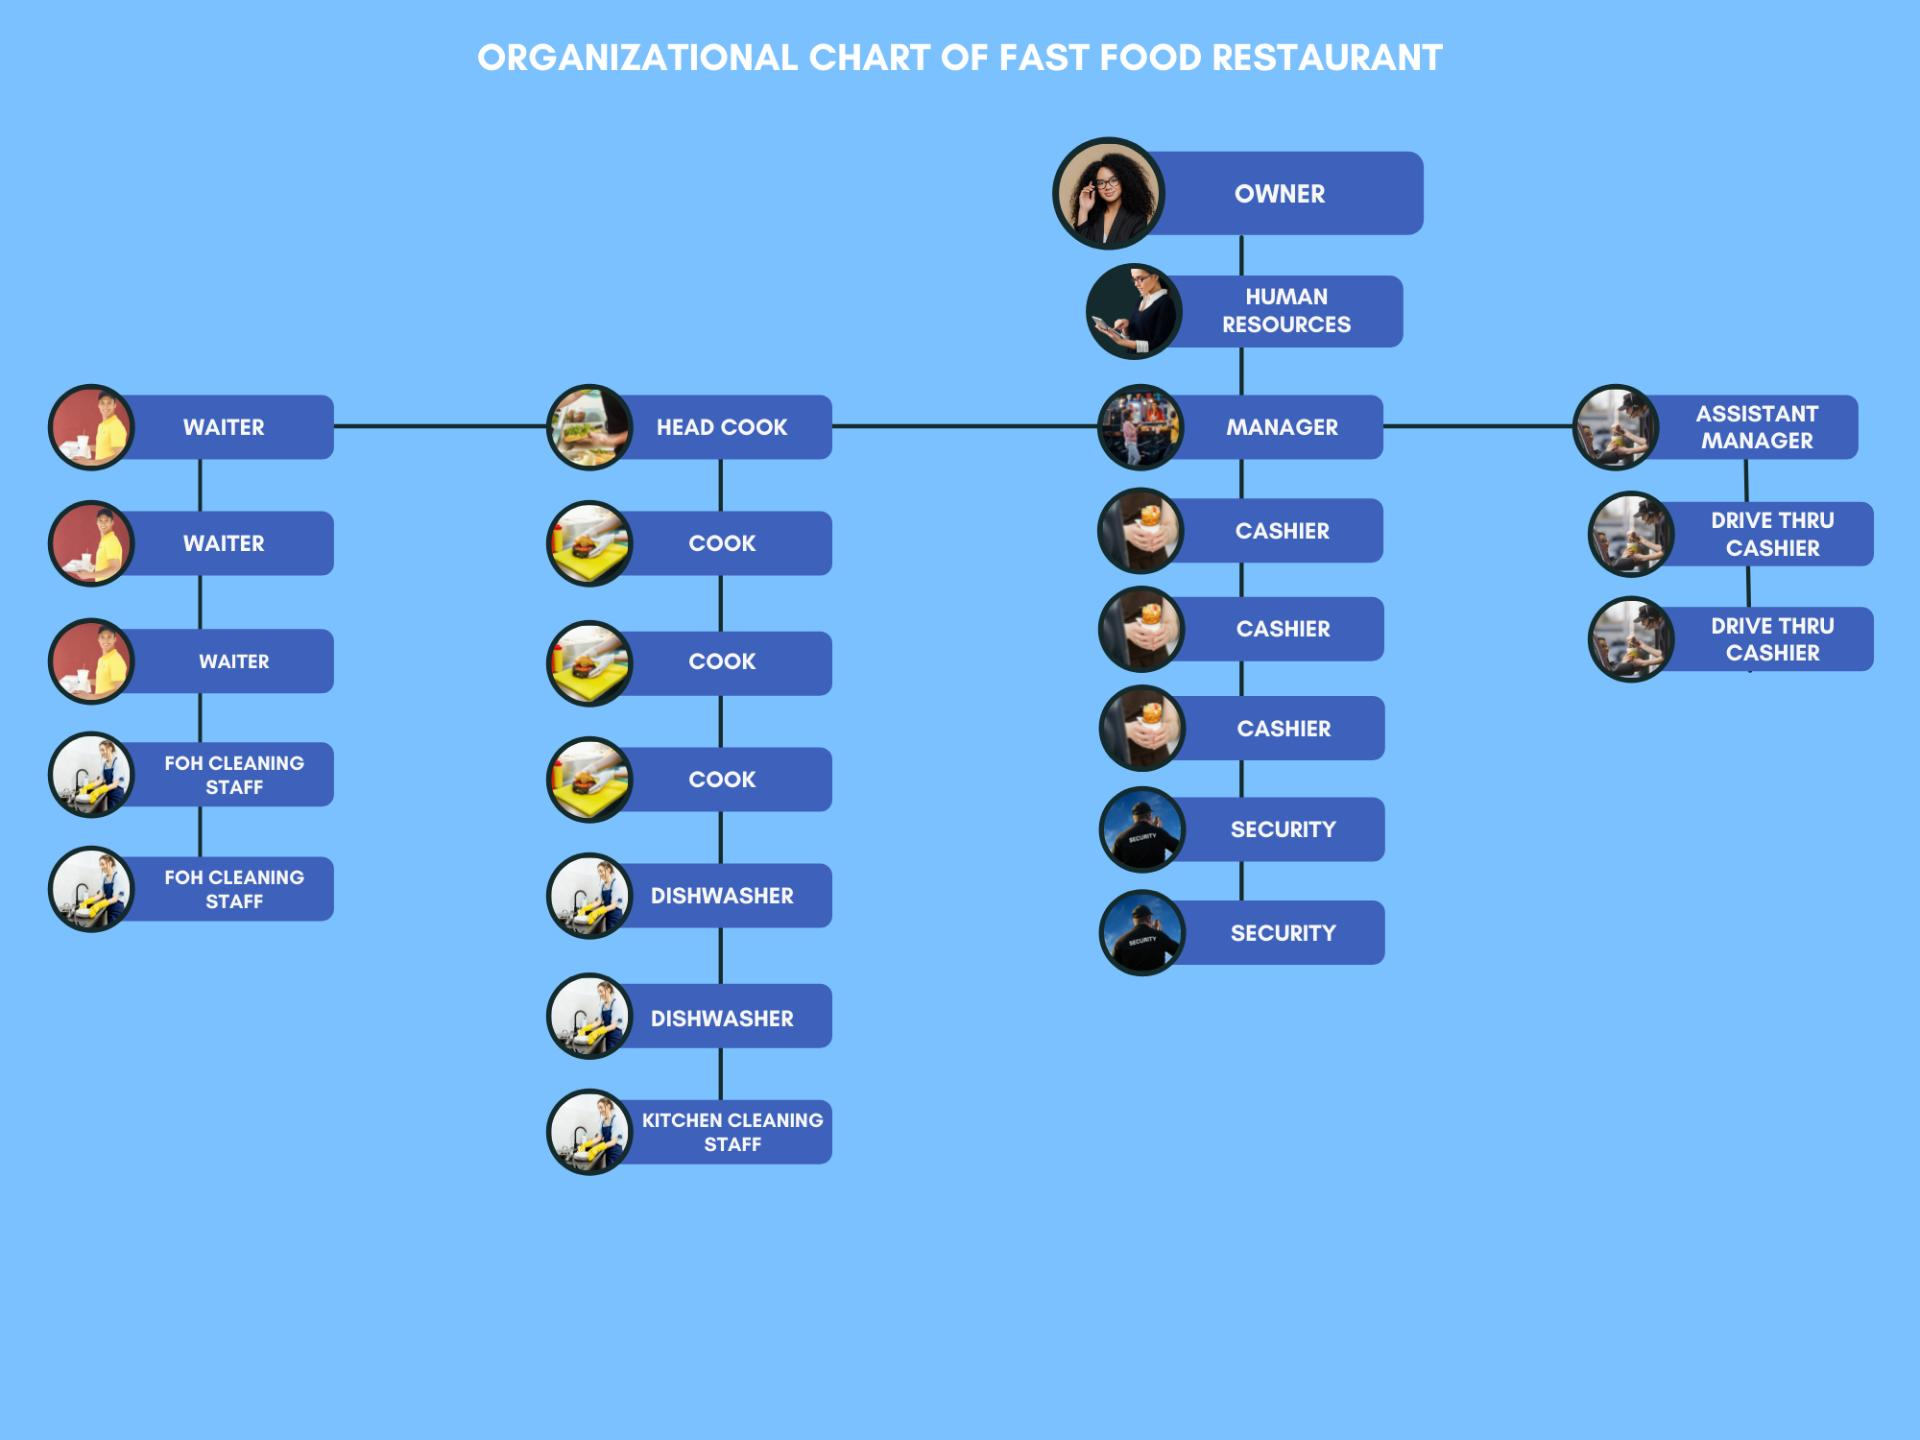
\includegraphics[width=15cm]{Images/fast-food-org-chart.jpg}
	\vspace{0.5cm}
	\caption{Sơ đồ tổ chức cho nhà hàng phục vụ đồ ăn nhanh. Nguồn: waiterio.com}
\end{figure}


\subsubsection{Sự khác nhau giữa nhà hàng ăn uống cao cấp và nhà hàng phục vụ đồ ăn nhanh}

\subsection*{Bảng so sánh tổng quan}

\begin{longtable}{| m{3.5cm} | >{\RaggedRight}m{6.5cm} | >{\RaggedRight}m{6.5cm} |}
	\caption{Bảng so sánh giữa nhà hàng phục vụ đồ ăn cao cấp và nhà hàng phục vụ đồ ăn nhanh} \label{tab:comparison_detail}                                                                                                                                                                                                                                                                                                                                                                                                                                                                                         \\
	\hline
	\textbf{Tiêu chí}                    & \textbf{Nhà hàng Fine Dining}                                                                                                                                                                                                                                                           & \textbf{Nhà hàng Fast Food (QSR)}                                                                                                                                                                                                                                               \\
	\hline
	\endfirsthead

	\hline
	\textbf{Tiêu chí}                    & \textbf{Nhà hàng Fine Dining}                                                                                                                                                                                                                                                           & \textbf{Nhà hàng Fast Food (QSR)}                                                                                                                                                                                                                                               \\
	\hline
	\endhead

	\hline
	\multicolumn{3}{|c|}{\textit{Còn tiếp}}                                                                                                                                                                                                                                                                                                                                                                                                                                                                                                                                                                          \\
	\hline
	\endfoot

	\hline
	\endlastfoot

	\textbf{Định nghĩa \& Khái niệm}     & Trải nghiệm nhà hàng tinh tế, thường đắt đỏ, đặc biệt hơn nhà hàng thông thường. Tập trung vào chất lượng cao và dịch vụ hoàn hảo.                                                                                                                                                      & Cơ sở cung cấp thức ăn được chuẩn bị và phục vụ nhanh chóng, thực đơn hạn chế, thường dùng đồ một lần. Tập trung vào tốc độ và sự tiện lợi.                                                                                                                                     \\
	\hline
	\textbf{Trải nghiệm Khách hàng}      & \begin{itemize} \item Sang trọng, độc quyền \item Dịch vụ cá nhân hóa, chu đáo tại bàn \item Không gian tinh tế, yên tĩnh \item Chú trọng từng chi tiết nhỏ \end{itemize}                                                                                                               & \begin{itemize} \item Nhanh chóng, tiện lợi \item Tự phục vụ hoặc đặt tại quầy/drive-thru \item Không gian chức năng, đôi khi ồn ào \item Ít chú trọng chi tiết trải nghiệm không gian \end{itemize}                                                                            \\
	\hline
	\textbf{Thực đơn}                    & \begin{itemize} \item Sáng tạo, phức tạp \item Nguyên liệu cao cấp, tươi ngon \item Thường có thực đơn cố định (set menu) hoặc gọi món (à la carte) phong phú \item Chịu ảnh hưởng lớn từ Bếp trưởng \end{itemize}                                                                      & \begin{itemize} \item Hạn chế, chuẩn hóa \item Nguyên liệu tập trung vào chi phí và tốc độ chế biến \item Thường là các món phổ biến (burger, gà rán, pizza, khoai tây chiên) \item Đồng nhất giữa các chi nhánh (nếu là chuỗi) \end{itemize}                                   \\
	\hline
	\textbf{Giá cả}                      & Cao cấp, phản ánh chất lượng nguyên liệu, kỹ năng chế biến, dịch vụ và không gian.                                                                                                                                                                                                      & Thấp, phù hợp với đại chúng, tập trung vào việc bán số lượng lớn.                                                                                                                                                                                                               \\
	\hline
	\textbf{Dịch vụ}                     & \begin{itemize} \item Dịch vụ tại bàn bởi nhân viên được đào tạo bài bản (waiters) \item Có Maitre d' chào đón và xếp chỗ \item Thường có Chuyên viên rượu (Sommelier) \item Tỷ lệ nhân viên/khách hàng cao \end{itemize}                                                               & \begin{itemize} \item Tự phục vụ hoặc dịch vụ tại quầy/drive-thru \item Nhân viên thực hiện các tác vụ nhanh gọn (nhận order, thu tiền, giao đồ ăn) \item Ít tương tác cá nhân hóa \item Tỷ lệ nhân viên/khách hàng thấp \end{itemize}                                          \\
	\hline
	\textbf{Không gian \& Thiết kế}      & Sang trọng, đầu tư vào nội thất, ánh sáng, âm nhạc, bộ đồ ăn. Thường dùng khăn trải bàn trắng.                                                                                                                                                                                          & Chức năng, hiệu quả, dễ lau dọn. Thiết kế thường theo chuẩn thương hiệu (nếu là chuỗi). Ít chú trọng yếu tố sang trọng.                                                                                                                                                         \\
	\hline
	\textbf{Mô hình Kinh doanh}          & \begin{itemize} \item Chi phí vận hành rất cao (nguyên liệu, nhân sự tay nghề cao, mặt bằng đắc địa) \item Biên lợi nhuận có thể cao trên từng món nhưng tổng thể lợi nhuận là thách thức \item Phụ thuộc vào danh tiếng, đánh giá (sao Michelin), khách hàng trung thành \end{itemize} & \begin{itemize} \item Chi phí vận hành thấp hơn trên từng đơn vị sản phẩm \item Biên lợi nhuận thấp trên từng món, dựa vào bán số lượng cực lớn \item Thường hoạt động theo mô hình chuỗi, nhượng quyền (franchise) \item Marketing và nhận diện thương hiệu mạnh \end{itemize} \\
	\hline
	\textbf{Hoạt động Vận hành}          & \begin{itemize} \item Quy trình chuẩn bị món ăn phức tạp, đòi hỏi kỹ năng cao \item Chú trọng kiểm soát chất lượng từng đĩa ăn \item Quản lý tồn kho nguyên liệu cao cấp phức tạp \end{itemize}                                                                                         & \begin{itemize} \item Quy trình tinh giản, dây chuyền hóa \item Sử dụng công nghệ (POS, KDS) để tối ưu tốc độ \item Chuỗi cung ứng tập trung, hiệu quả \item Đào tạo nhân viên tập trung vào tốc độ, chính xác \end{itemize}                                                    \\
	\hline
	\textbf{Nhân sự \& Cấu trúc Tổ chức} & \begin{itemize} \item Đội ngũ lớn, nhiều vị trí chuyên môn hóa cao (Bếp trưởng, Bếp phó, Đầu bếp chuyên khoa, Maitre d', Sommelier, Quản lý) \item Cấu trúc tổ chức phức tạp, đa tầng \item Yêu cầu kỹ năng và kinh nghiệm cao \end{itemize}                                            & \begin{itemize} \item Đội ngũ tinh gọn hơn, các vai trò ít chuyên môn hóa hơn (Quản lý ca, Thu ngân, Nhân viên bếp, Nhân viên vệ sinh) \item Cấu trúc tổ chức phẳng, đơn giản \item Đào tạo tập trung vào quy trình chuẩn, dễ thay thế \end{itemize}                            \\
	\hline
	\textbf{Mục tiêu chính}              & Cung cấp trải nghiệm ẩm thực đỉnh cao, độc đáo, xây dựng danh tiếng và thương hiệu đẳng cấp.                                                                                                                                                                                            & Tối đa hóa tốc độ phục vụ, sự tiện lợi, khối lượng bán và lợi nhuận thông qua hiệu quả vận hành.                                                                                                                                                                                \\
	\hline
\end{longtable}


Sự tương phản giữa nhà hàng fine dining và fast food không chỉ dừng lại ở các yếu tố bề mặt như giá cả hay tốc độ. Nó bắt nguồn từ triết lý kinh doanh, đối tượng khách hàng mục tiêu, và mô hình vận hành hoàn toàn khác biệt, dẫn đến những hệ quả sâu sắc:

\begin{itemize}
	\item \textbf{Giá trị cốt lõi:} Fine dining bán một \textit{trải nghiệm toàn diện}, nơi ẩm thực chỉ là một phần (dù là phần quan trọng nhất). Các yếu tố như không gian, dịch vụ cá nhân hóa, sự độc quyền, và cảm giác được chăm sóc đặc biệt đóng góp lớn vào giá trị mà khách hàng nhận được và sẵn sàng chi trả cao. Ngược lại, fast food bán \textit{sự tiện lợi và tính nhất quán}. Khách hàng tìm đến vì tốc độ, giá cả phải chăng và biết chính xác họ sẽ nhận được gì ở bất kỳ chi nhánh nào của thương hiệu.

	\item \textbf{Rủi ro và Lợi nhuận:} Mô hình fine dining có rủi ro cao hơn do chi phí đầu tư và vận hành lớn, cùng sự phụ thuộc vào danh tiếng và lượng khách hàng giới hạn. Một đánh giá tiêu cực hoặc thay đổi xu hướng ẩm thực có thể ảnh hưởng nghiêm trọng. Tuy nhiên, khi thành công, biên lợi nhuận trên mỗi khách hàng có thể rất cao. Fast food có rủi ro thấp hơn trên từng giao dịch nhờ mô hình chuẩn hóa và khối lượng lớn. Lợi nhuận đến từ việc tối ưu hóa chi phí và quy mô, nhưng lại nhạy cảm với cạnh tranh về giá và chi phí nguyên liệu đầu vào.

	\item \textbf{Vai trò của Con người và Công nghệ:} Trong fine dining, yếu tố con người là không thể thay thế. Kỹ năng của đầu bếp, sự tinh tế của nhân viên phục vụ, và kiến thức của sommelier tạo nên sự khác biệt. Công nghệ chủ yếu hỗ trợ quản lý (đặt bàn, POS) chứ không thay thế vai trò trung tâm của con người trong việc tạo ra trải nghiệm. Ngược lại, fast food tận dụng tối đa công nghệ để \textit{tăng hiệu suất và giảm sự phụ thuộc vào kỹ năng cá nhân}. Từ hệ thống đặt hàng tự động, bếp dây chuyền, đến phân tích dữ liệu bán hàng, công nghệ là chìa khóa để duy trì tốc độ và sự đồng nhất.

	\item \textbf{Cấu trúc tổ chức phản ánh sự phức tạp:} Sơ đồ tổ chức đa tầng của fine dining cho thấy sự chuyên môn hóa cao độ cần thiết để duy trì chất lượng ở mọi khâu, từ bếp đến tiền sảnh. Mỗi vị trí có vai trò và trách nhiệm rõ ràng, đòi hỏi kỹ năng chuyên biệt. Cấu trúc phẳng của fast food phản ánh quy trình làm việc đơn giản, lặp lại và tập trung vào hiệu quả hoạt động theo ca dưới sự giám sát của quản lý ca.

	\item \textbf{Thích ứng và Xu hướng:} Cả hai mô hình đều đang phải thích ứng. Fine dining ngày càng chú trọng hơn đến tính bền vững, nguồn gốc nguyên liệu và trải nghiệm độc đáo (ví dụ: bếp mở, tương tác với đầu bếp). Một số nhà hàng fine dining cũng tìm cách tiếp cận phân khúc rộng hơn thông qua các mô hình "casual dining" hoặc "bistro" cao cấp. Fast food đang đối mặt với áp lực về thực phẩm lành mạnh hơn, nguồn gốc rõ ràng và trải nghiệm khách hàng tốt hơn (không gian sạch đẹp, dịch vụ thân thiện hơn). Sự trỗi dậy của "fast-casual" (phân khúc giữa fast food và casual dining) là minh chứng cho sự thay đổi này, kết hợp tốc độ của fast food với chất lượng nguyên liệu và không gian tốt hơn.

\end{itemize}

\subsection{Hành trình khách hàng (Customer Journey) trong ngành dịch vụ nhà hàng}

Hành trình khách hàng trong ngành dịch vụ nhà hàng là một chuỗi các tương tác và trải nghiệm, từ giai đoạn nhận thức ban đầu đến hành động quay lại sử dụng dịch vụ. Hiểu rõ và tối ưu hóa từng giai đoạn trong hành trình này là yếu tố then chốt để nâng cao sự hài lòng của khách hàng, xây dựng lòng trung thành và tạo lợi thế cạnh tranh bền vững cho nhà hàng. Theo Orderable \cite{Orderable}, hành trình khách hàng trong ngành dịch vụ nhà hàng có thể chia thành các cột mốc như sau:

\begin{figure}[H]
	\centering
	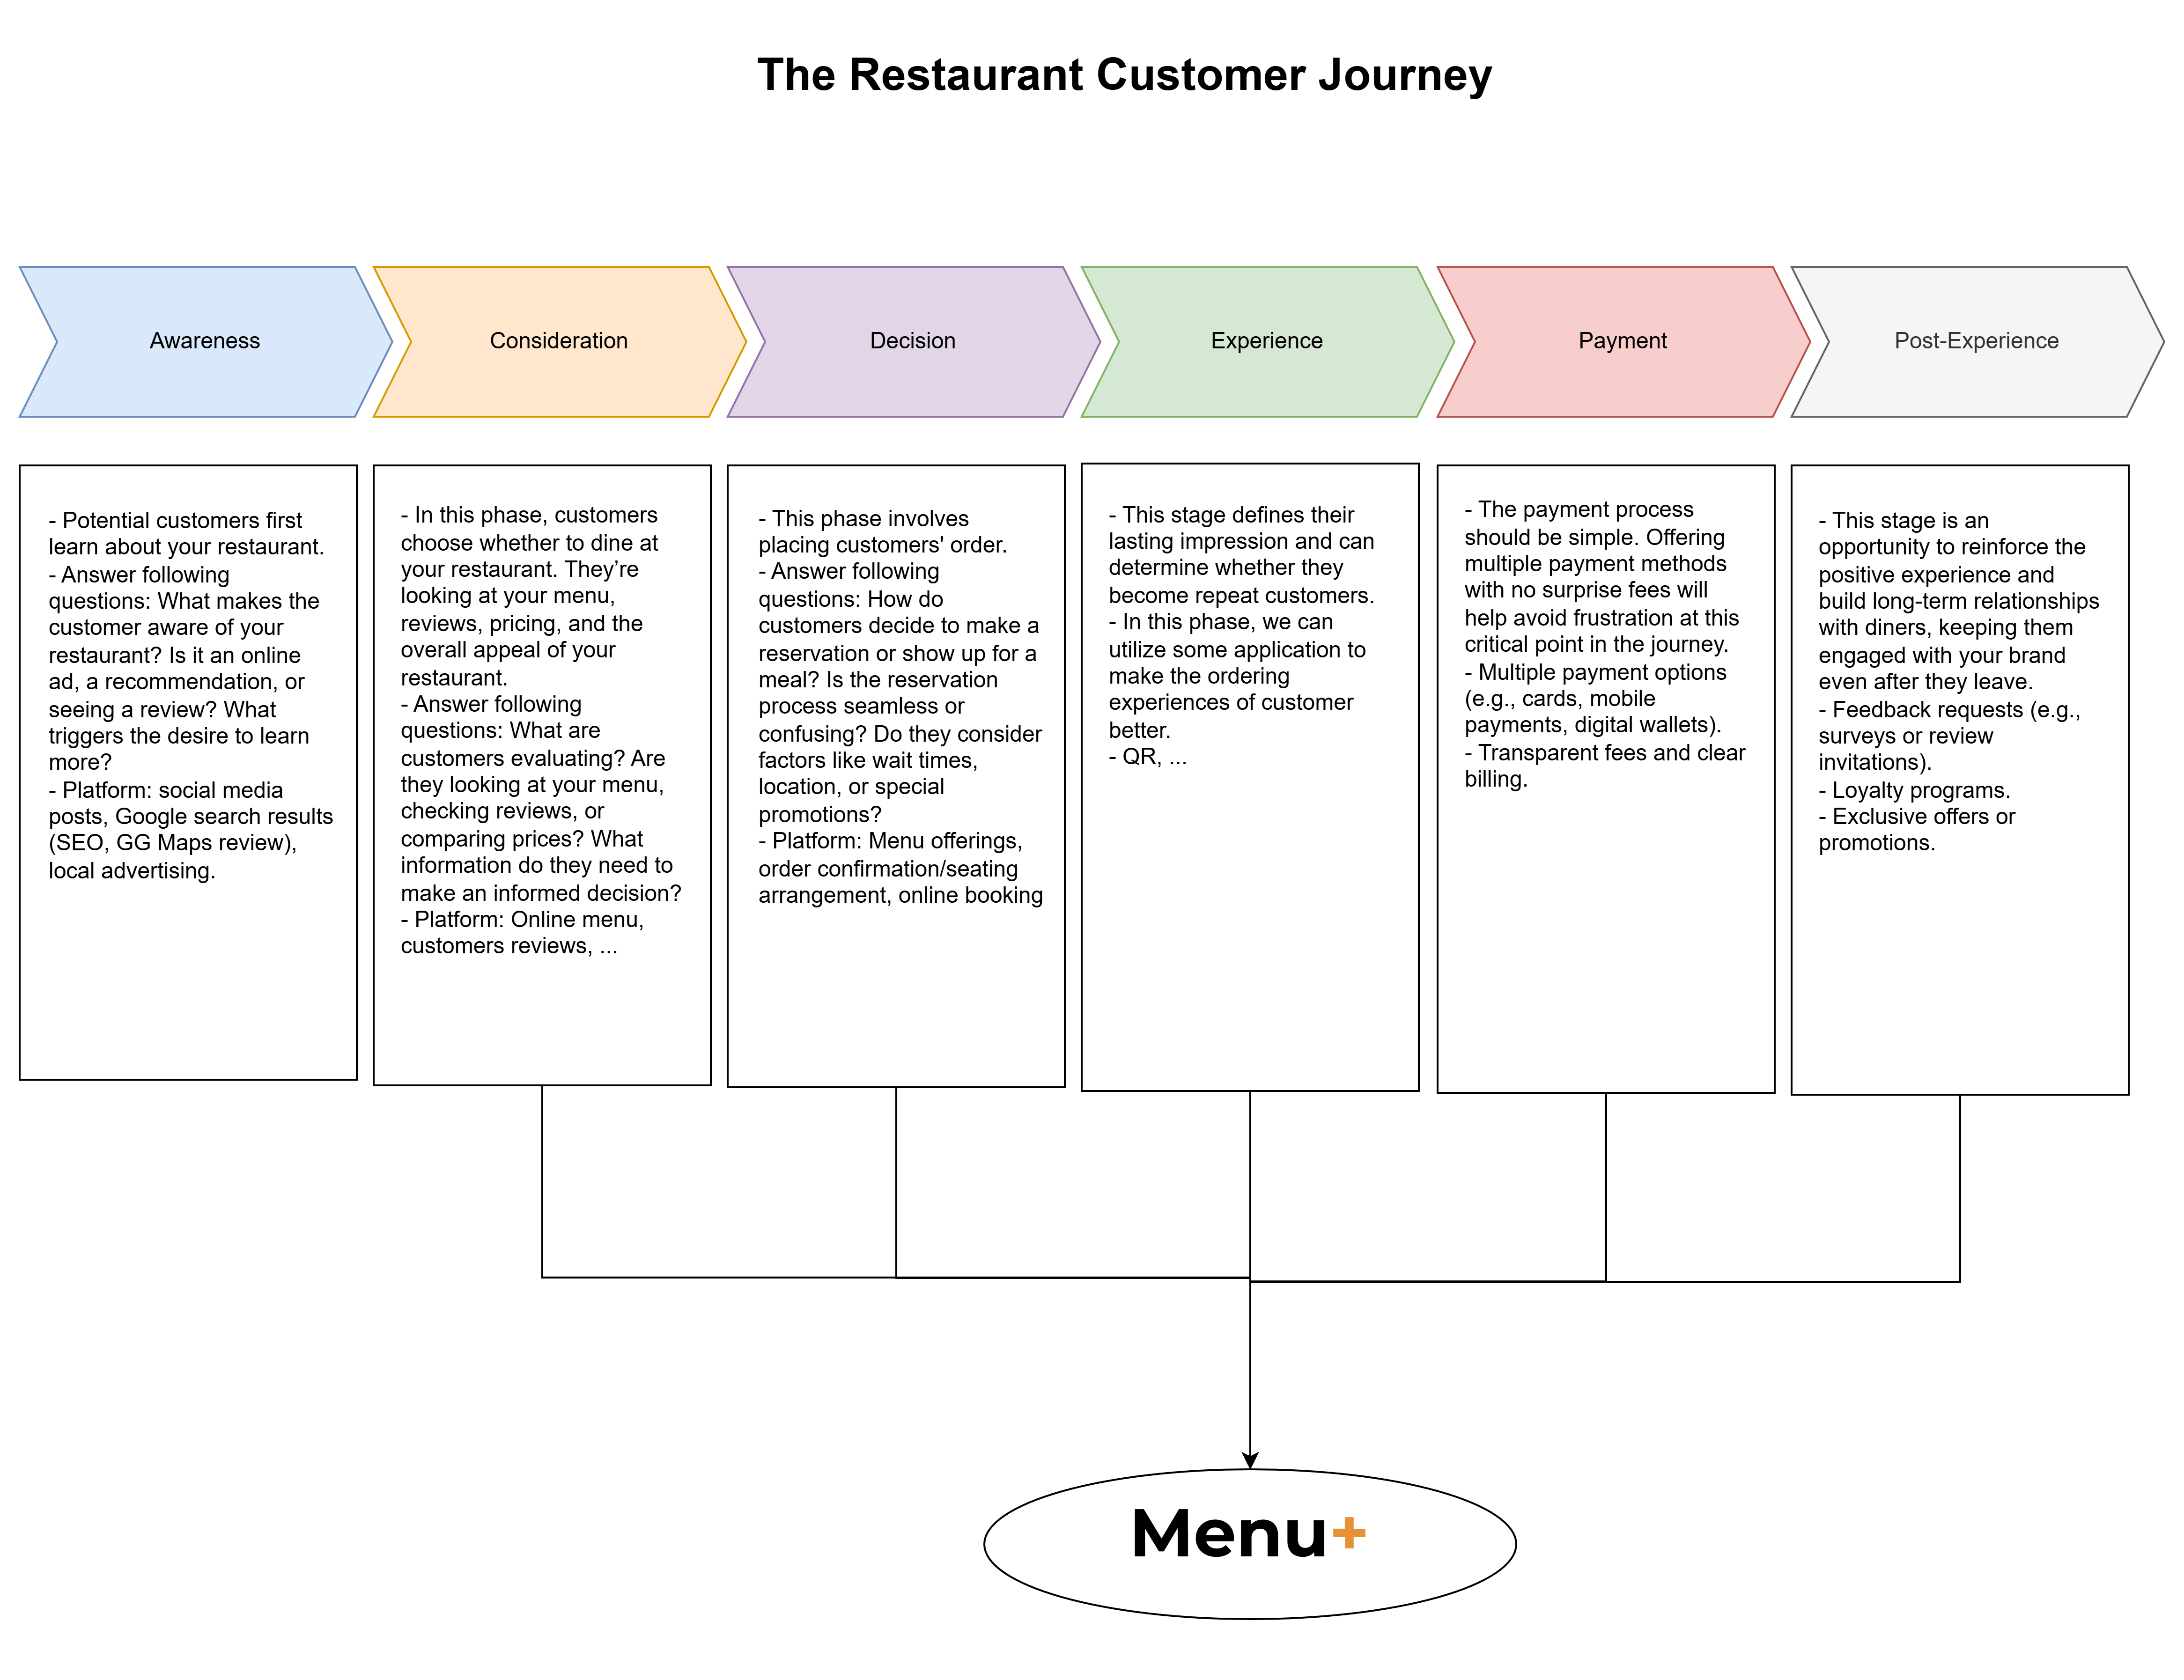
\includegraphics[width=15cm]{Images/restaurant-customer-journey.png}
	\caption{Giới thiệu về Hành trình Khách hàng trong Nhà hàng.}
	\label{fig:my_label}
\end{figure}

\begin{enumerate}
	\item Giai đoạn Nhận thức (Awareness): Giai đoạn này đánh dấu điểm tiếp xúc đầu tiên của khách hàng tiềm năng với nhà hàng. Các kênh truyền thông đa dạng, từ quảng cáo trực tuyến (ví dụ: Google Ads, quảng cáo trên mạng xã hội), đánh giá trực tuyến (ví dụ: Google Reviews, TripAdvisor), đến các phương pháp truyền thống như quảng cáo in ấn, giới thiệu từ người thân, đóng vai trò quan trọng trong việc tạo dựng nhận diện thương hiệu.
	\item Giai đoạn Cân nhắc (Consideration): Sau khi nhận biết về nhà hàng, khách hàng tiềm năng sẽ tiến hành thu thập thông tin chi tiết hơn, so sánh với các lựa chọn khác. Họ sẽ xem xét thực đơn, bảng giá, hình ảnh không gian, đọc các đánh giá chi tiết và có thể tham khảo ý kiến từ bạn bè, người thân.
	\item Giai đoạn Quyết định (Decision): Giai đoạn này là thời điểm khách hàng đưa ra quyết định lựa chọn nhà hàng. Các yếu tố ảnh hưởng đến quyết định bao gồm sự thuận tiện trong việc đặt bàn, vị trí địa lý, đánh giá tổng quan về nhà hàng, và các chương trình khuyến mãi, ưu đãi đặc biệt.
	\item Giai đoạn Trải nghiệm (Experience): Đây là giai đoạn quan trọng nhất, khi khách hàng trực tiếp trải nghiệm dịch vụ và sản phẩm tại nhà hàng. Chất lượng món ăn, thái độ phục vụ, không gian nhà hàng, sự sạch sẽ và tiện nghi đều đóng vai trò then chốt. Việc ứng dụng công nghệ, ví dụ như hệ thống gọi món, thanh toán không tiền mặt, có thể nâng cao trải nghiệm khách hàng.
	\item Giai đoạn Thanh toán (Payment): Quá trình thanh toán cần được thực hiện nhanh chóng, chính xác và thuận tiện. Cung cấp đa dạng các phương thức thanh toán (ví dụ: tiền mặt, thẻ tín dụng, ví điện tử) để đáp ứng nhu cầu của khách hàng.
	\item Giai đoạn Hậu trải nghiệm (Post-Experience): Sau khi khách hàng rời nhà hàng, việc duy trì kết nối và khuyến khích quay lại là rất quan trọng. Gửi email cảm ơn, mời tham gia khảo sát đánh giá, cung cấp các chương trình khách hàng thân thiết, và gửi các ưu đãi đặc biệt là những phương pháp hiệu quả.
\end{enumerate}

\subsection{Mô hình MVC}
MVC là viết tắt của khái niệm "Model-View-Controller", một trong những mô hình thiết kế phần mềm phổ biến nhất.\\

MVC tách biệt dữ liệu, giao diện người dùng và logic xử lý thành ba thành phần riêng biệt nhưng vẫn được kết nối chặt chẽ với nhau.

\begin{itemize}
	\item Model (M): Đại diện cho dữ liệu và logic xử lý các nghiệp vụ của ứng dụng.
	\item View (V): Quản lý giao diện và hiển thị dữ liệu ra cho người dùng.
	\item Controller (C): Làm điều phối và điều hướng tương tác giữa Model và View. Nó nhận yêu cầu từ View, thực hiện xử lý trên Model và trả kết quả về cho View hiển thị.
\end{itemize}

MVC giúp tách biệt các thành phần của ứng dụng, tăng tính bảo trì và khả năng mở rộng trong tương lai \cite{MVC}.

\begin{figure}[H]
	\centering
	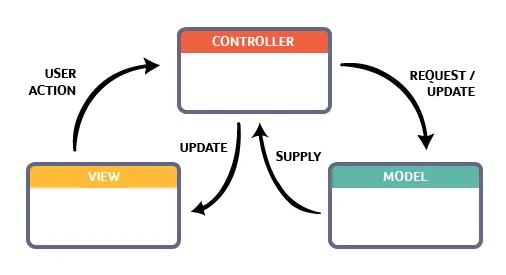
\includegraphics[width=10cm]{Images/ezgif-4-c53032b3fd.png}
	\vspace{0.5cm}
	\caption{MVC là gì? Nguồn: \href{https://viblo.asia/p/ios-mot-so-cach-co-ban-de-truyen-du-lieu-tu-model-toi-controller-trong-mo-hinh-mvc-L4x5xNWqZBM}{viblo.asia}}
	\label{fig:my_label}
\end{figure}

Mô hình MVC (MVC pattern) thường được dùng để phát triển giao diện người dùng. Nó cung cấp các thành phần cơ bản để thiết kế một chương trình cho máy tính hoặc điện thoại di động, cũng như là các ứng dụng web.

\subsubsection{Các thành phần của MVC}
Mô hình MVC gồm 3 loại chính là thành phần bên trong không thể thiếu khi áp dụng mô hình này:
\begin{figure}[H]
	\centering
	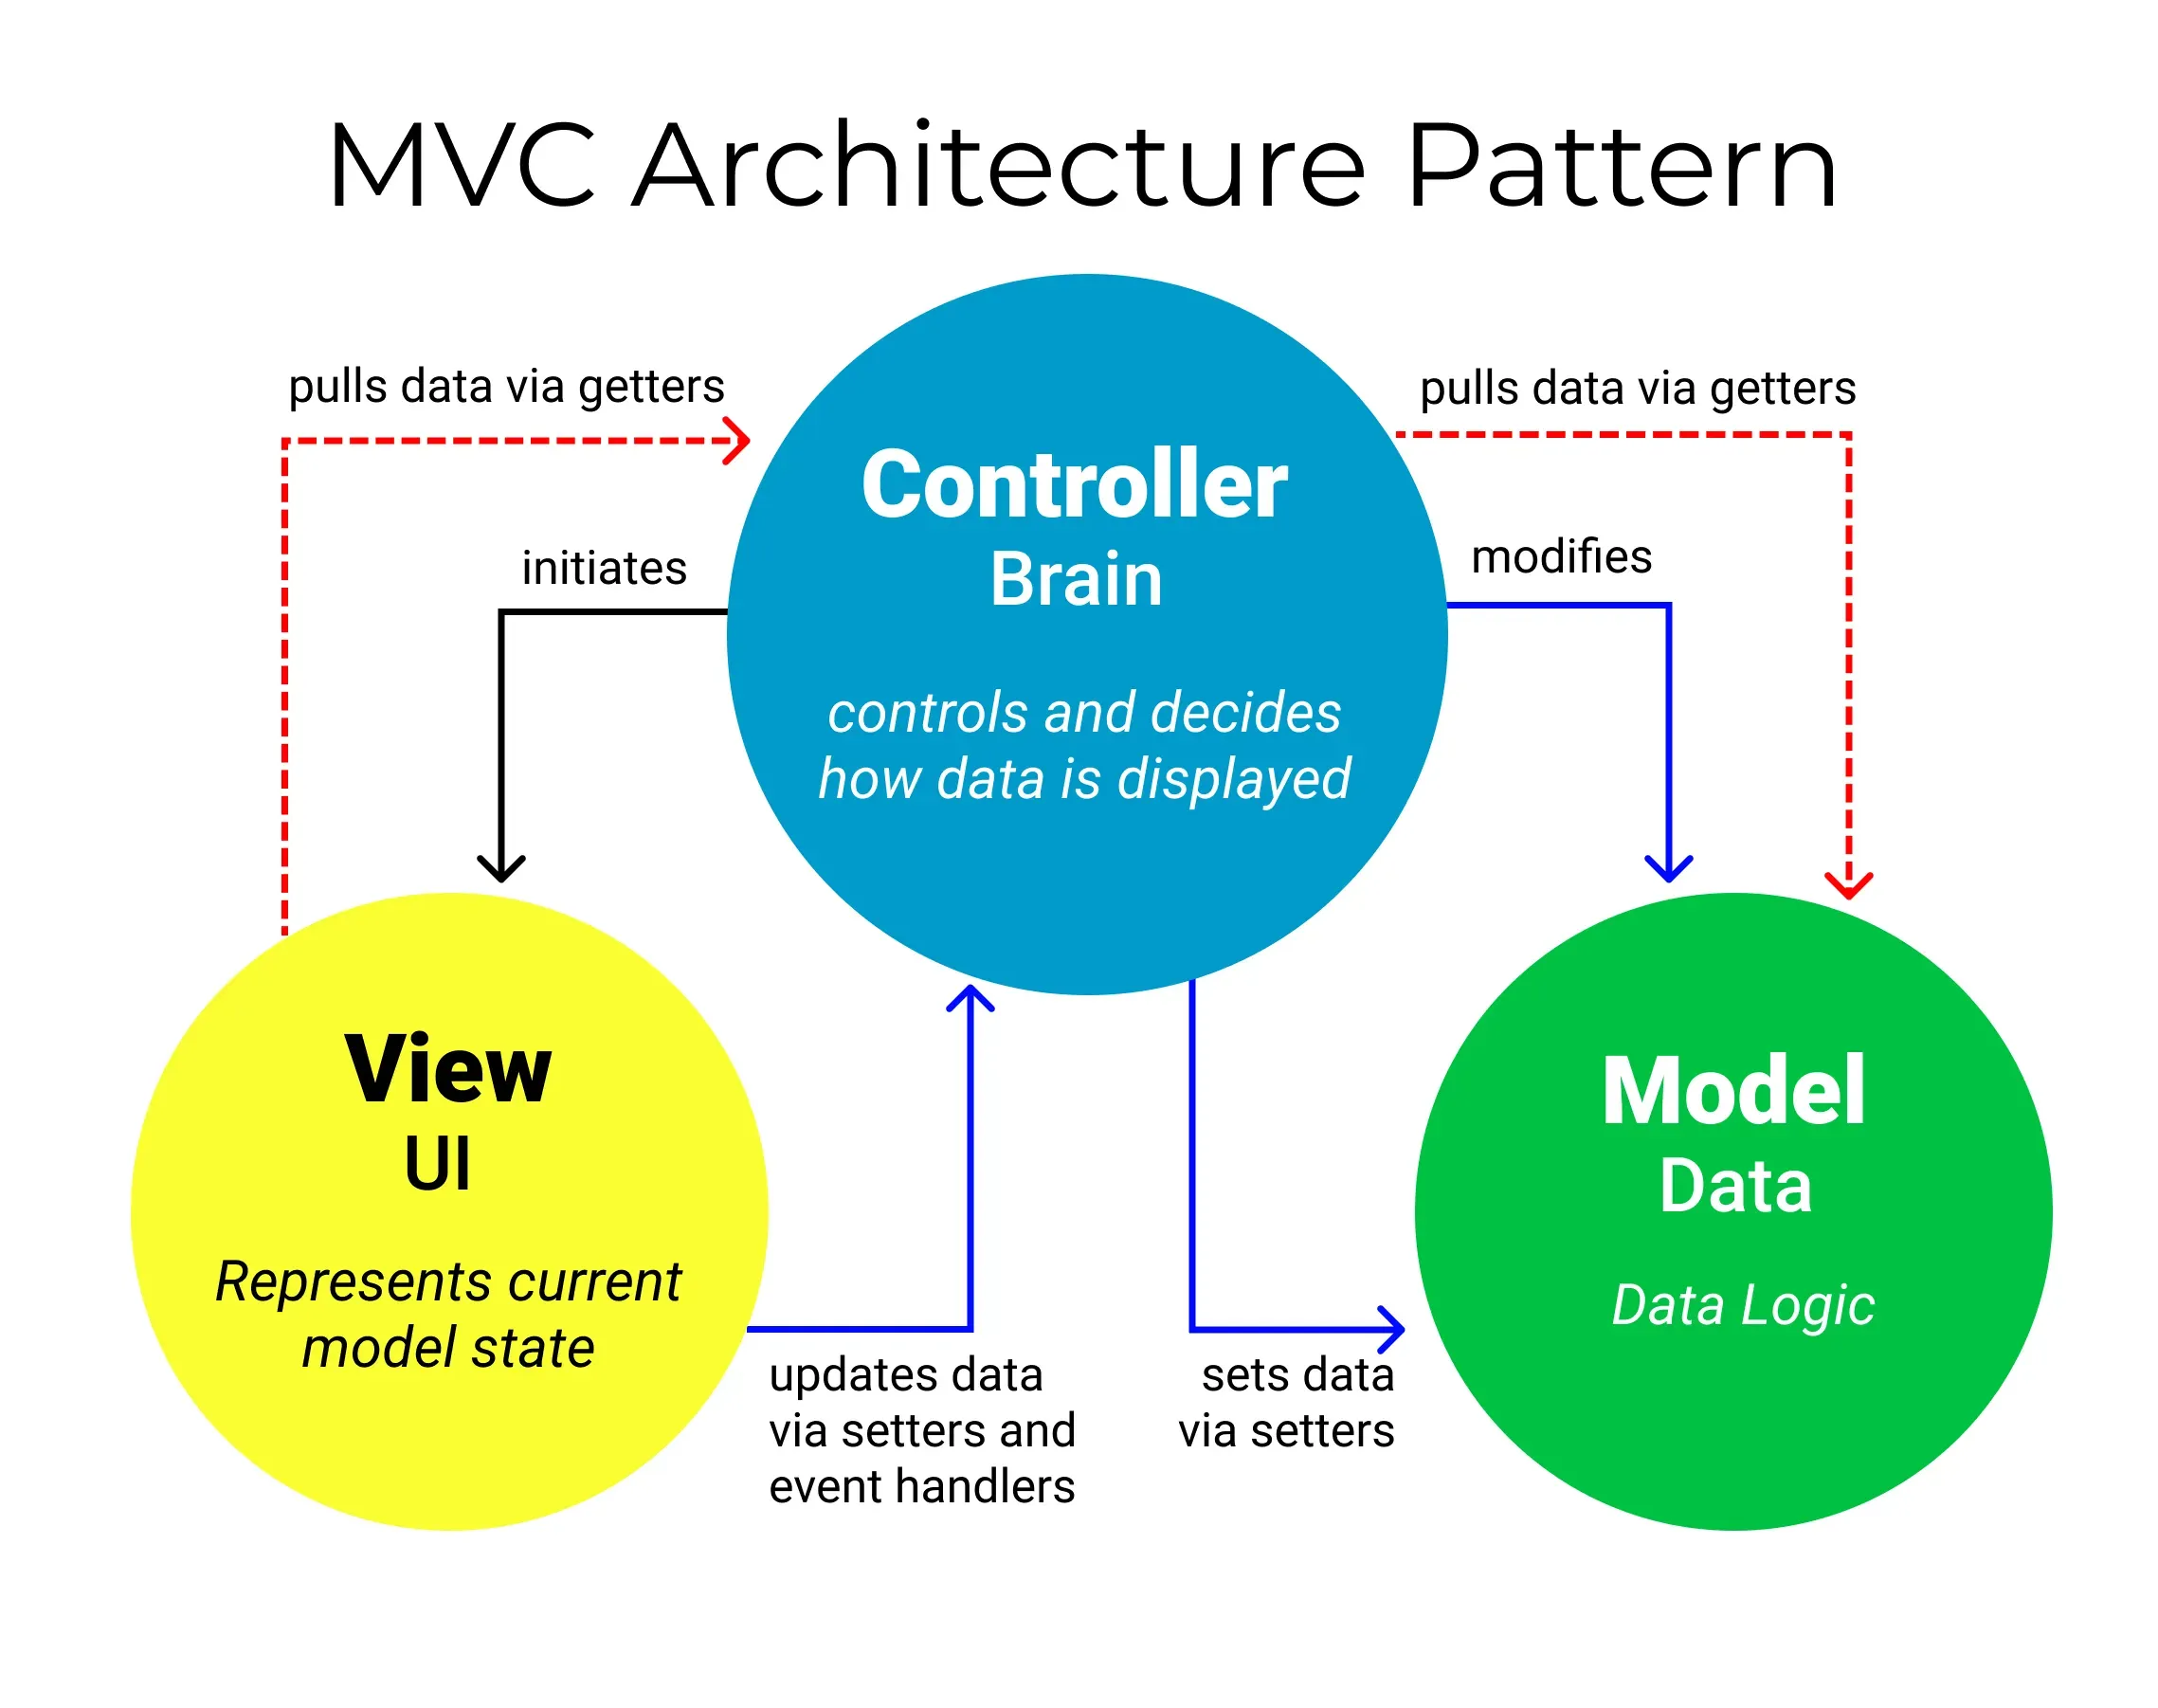
\includegraphics[width=10cm]{Images/cacthanhphanmvc.png}
	\vspace{0.5cm}
	\caption{Thành phần của MVC. Nguồn: \href{https://mhhj.tistory.com/m/95}{mhhj.tistory.com}}
	\label{fig:my_label}
\end{figure}

\begin{itemize}
	\item Model: Là bộ phận có chức năng lưu trữ toàn bộ dữ liệu của ứng dụng và là cầu nối giữa 2 thành phần bên dưới là View và Controller. Một model là dữ liệu được sử dụng bởi chương trình. Đây có thể là cơ sở dữ liệu, hoặc file XML bình thường hay một đối tượng đơn giản. Chẳng hạn như biểu tượng hay là một nhân vật trong game.
	\item View: Đây là phần giao diện (theme) dành cho người sử dụng. View là phương tiện hiển thị các đối tượng trong một ứng dụng. Chẳng hạn như hiển thị một cửa sổ, nút hay văn bản trong một cửa sổ khác. Nó bao gồm bất cứ thứ gì mà người dùng có thể nhìn thấy được.
	\item Controller: Là bộ phận có nhiệm vụ xử lý các yêu cầu người dùng đưa đến thông qua View. Một controller bao gồm cả Model lẫn View. Nó nhận input và thực hiện các update tương ứng.
\end{itemize}

\subsubsection{Luồng xử lý trong MVC}
Luồng xử lý trong của mô hình MVC, bạn có thể hình dung cụ thể và chi tiết qua từng bước dưới đây:
\begin{itemize}
	\item Khi một yêu cầu của từ máy khách (Client) gửi đến Server. Thì bị Controller trong MVC chặn lại để xem đó là URL request hay sự kiện.
	\item Sau đó, Controller xử lý input của user rồi giao tiếp với Model trong MVC.
	\item Model chuẩn bị data và gửi lại cho Controller.
	\item Cuối cùng, khi xử lý xong yêu cầu thì Controller gửi dữ liệu trở lại View và hiển thị cho người dùng trên trình duyệt.
\end{itemize}
\begin{figure}[H]
	\centering
	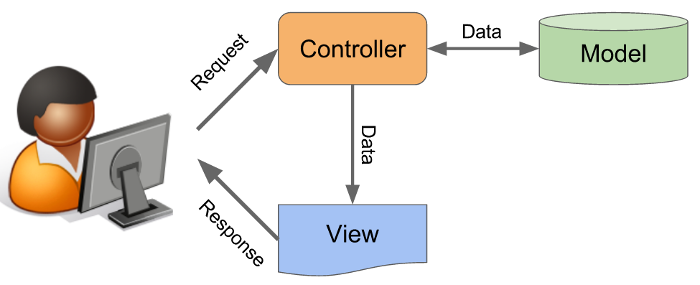
\includegraphics[width=10cm]{Images/luongmvc.png}
	\vspace{0.5cm}
	\caption{View và Model sẽ được xử lý bởi Controller. Nguồn: \href{https://dev.to/michellebuchiokonicha/the-model-view-controller-mvc-software-architectural-design-pattern-4jjd}{dev.to}}
	\label{fig:my_label}
\end{figure}

Ở đây, View không giao tiếp trực tiếp với Model. Sự tương tác giữa View và Model sẽ chỉ được xử lý bởi Controller.
% \newpage
% \section{CÁC HỆ THỐNG LIÊN QUAN}
\subsection{Ristorante Cracco}

\begin{figure}[H]
    \centering
    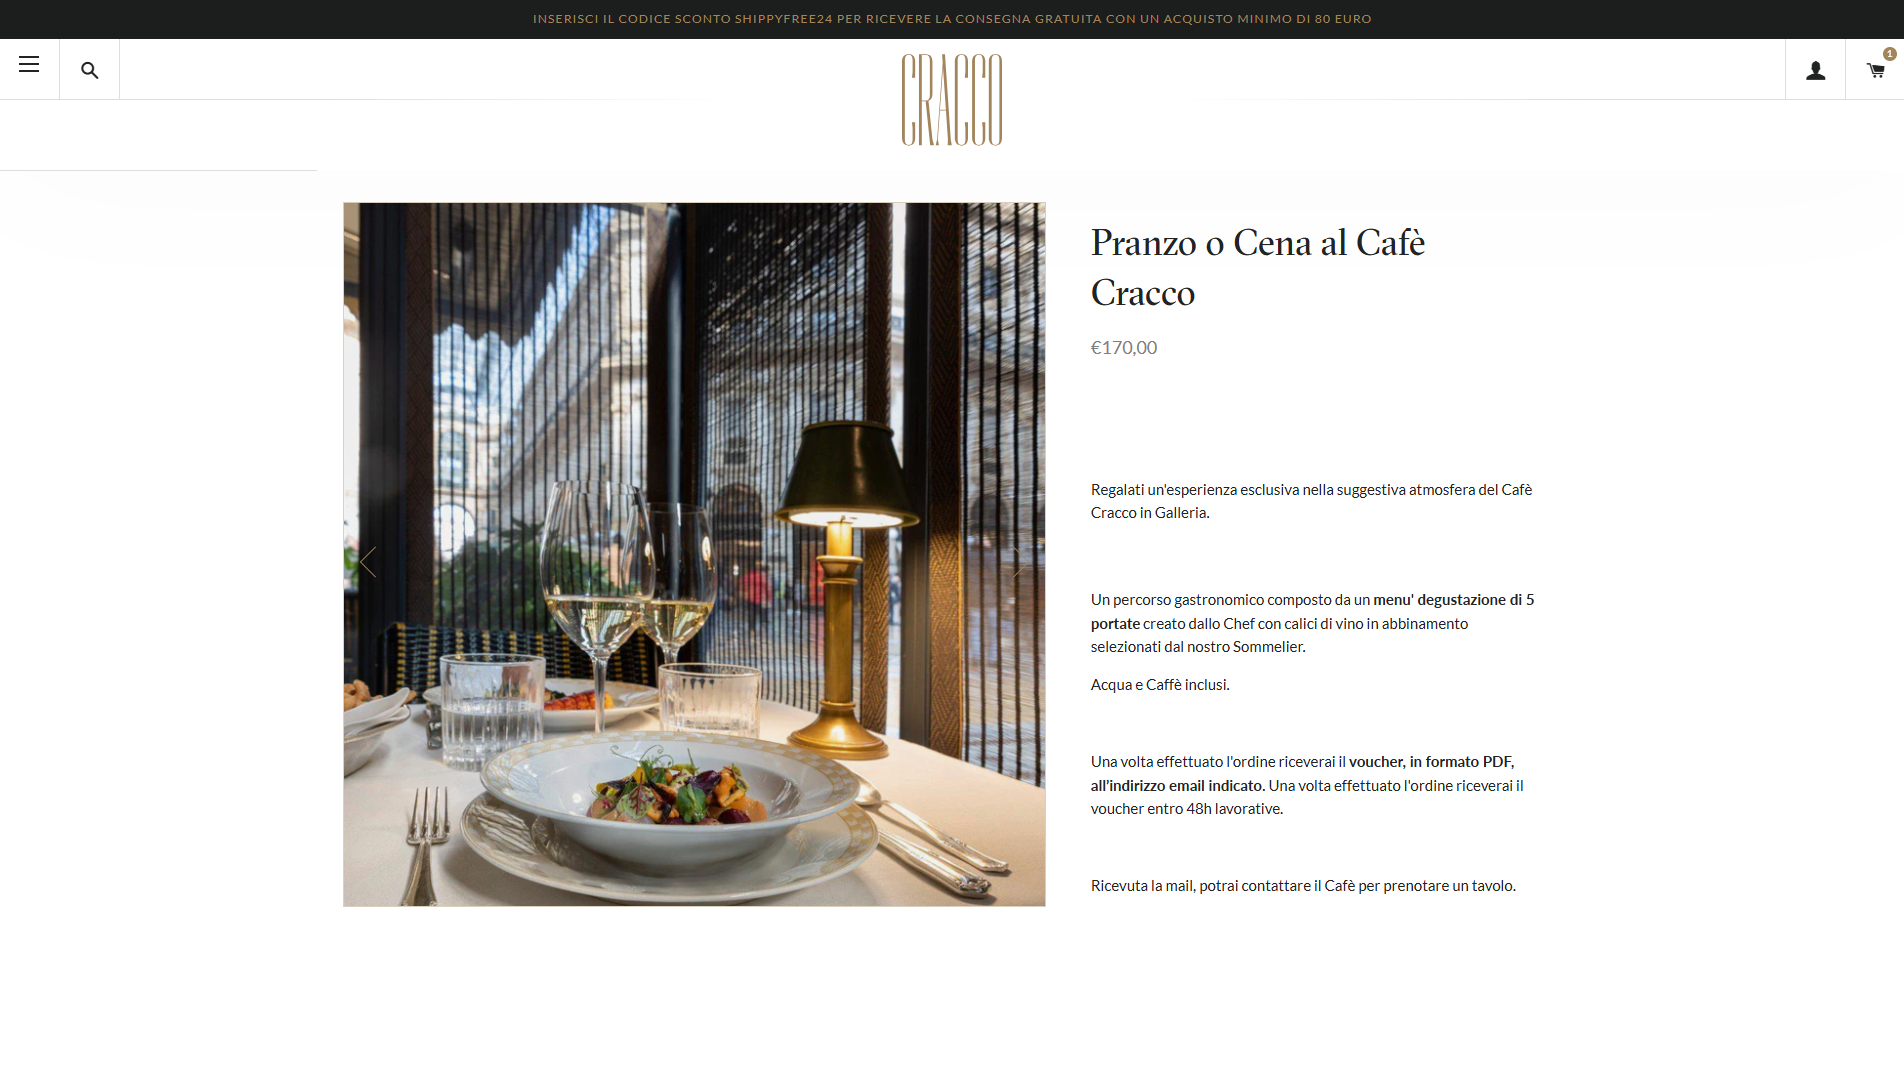
\includegraphics[width=15cm]{Images/ristorante_cracco.png}
    \vspace{0.5cm}
    \caption{Giao diện website Ristorante Cracco}
    \label{fig:my_label}
\end{figure}

Ristorante Cracco là một nhà hàng cao cấp tọa lạc tại trung tâm Milano, Ý, trong khu mua sắm lịch sử Galleria Vittorio Emanuele II. Được điều hành bởi đầu bếp danh tiếng Carlo Cracco, nhà hàng mang đến trải nghiệm ẩm thực tinh tế, kết hợp giữa truyền thống và sự sáng tạo hiện đại. Không gian của Ristorante Cracco trải rộng trên nhiều tầng, bao gồm nhà hàng chính, quán cà phê, hầm rượu và khu vực tổ chức sự kiện riêng. Thực đơn đa dạng với các món ăn độc đáo như súp cá bọc vỏ bánh và lòng đỏ trứng ngâm với măng tây và nấm cục đen, cùng với các món truyền thống như risotto nghệ với tủy xương nướng và ragù gan. Hầm rượu của nhà hàng chứa hơn 2.000 nhãn hiệu và hơn 10.000 chai rượu, chủ yếu từ Ý và Pháp. Trang web chính thức của Ristorante Cracco \href{https://www.ristorantecracco.it}{"https://www.ristorantecracco.it"} cung cấp thông tin chi tiết về thực đơn, đặt bàn trực tuyến và các sự kiện đặc biệt, giúp khách hàng dễ dàng tiếp cận và trải nghiệm dịch vụ đẳng cấp của nhà hàng.

\subsection{KFC Việt Nam}

\begin{figure}[H]
    \centering
    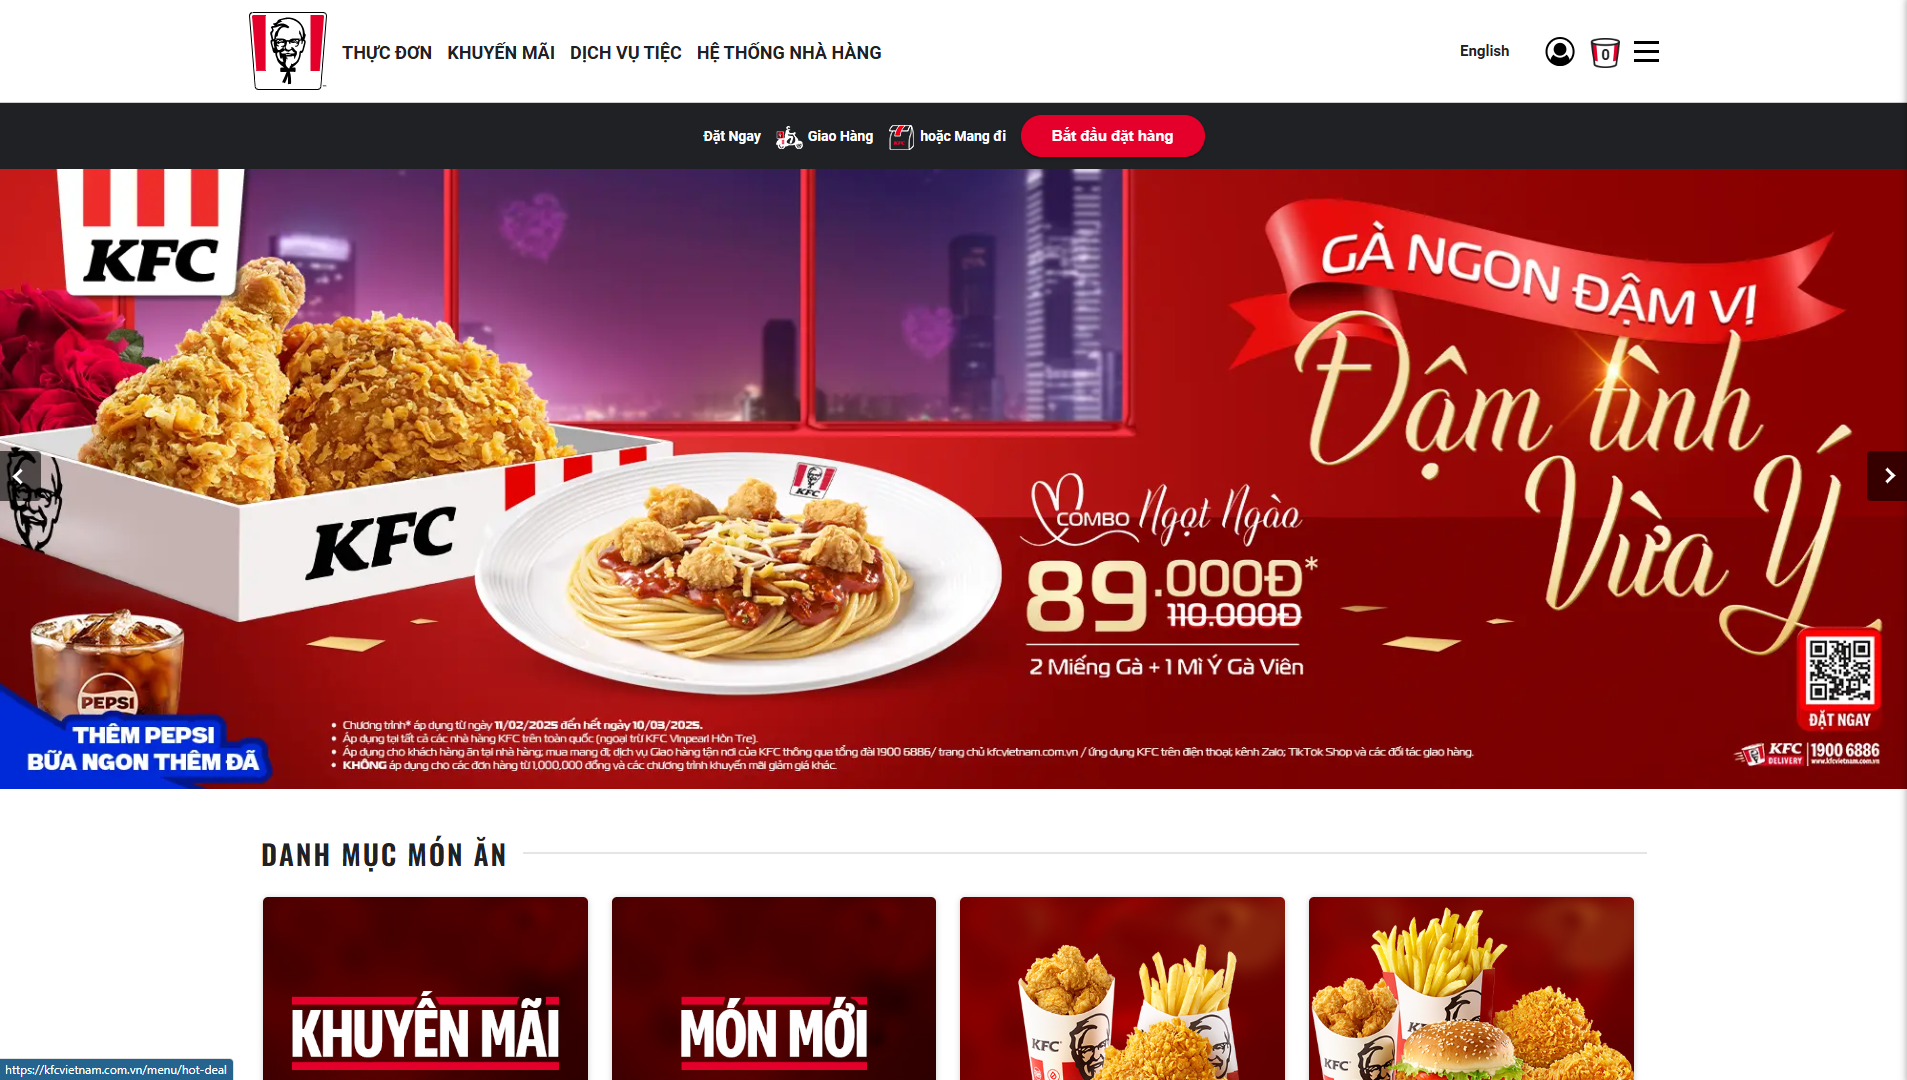
\includegraphics[width=15cm]{Images/kfc.png}
    \vspace{0.5cm}
    \caption{Giao diện website KFC Việt Nam}
    \label{fig:my_label}
\end{figure}

KFC Việt Nam là thành viên của tập đoàn Yum! Brands Inc. (Hoa Kỳ), chuyên cung cấp các sản phẩm gà rán và nướng, cùng với các món ăn kèm và sandwich chế biến từ thịt gà tươi. Kể từ khi khai trương nhà hàng đầu tiên tại TP. Hồ Chí Minh vào năm 1997, KFC đã mở rộng mạng lưới lên hơn 140 nhà hàng trên 21 tỉnh/thành phố, tạo việc làm cho hơn 3.000 lao động. Trang web chính thức của KFC Việt Nam \href{https://kfcvietnam.com.vn}{"https://kfcvietnam.com.vn"} cung cấp thông tin chi tiết về thực đơn đa dạng, bao gồm các món gà rán truyền thống và những món ăn được điều chỉnh phù hợp với khẩu vị Việt như Gà Big'n Juicy, Gà Giòn Không Xương, Cơm Gà KFC và Bắp Cải Trộn. Ngoài ra, trang web còn cập nhật các chương trình khuyến mãi, thông tin về nhà hàng và dịch vụ giao hàng trực tuyến, giúp khách hàng dễ dàng đặt món và tận hưởng hương vị KFC mọi lúc, mọi nơi.

\subsection{Haidilao}

\begin{figure}[H]
    \centering
    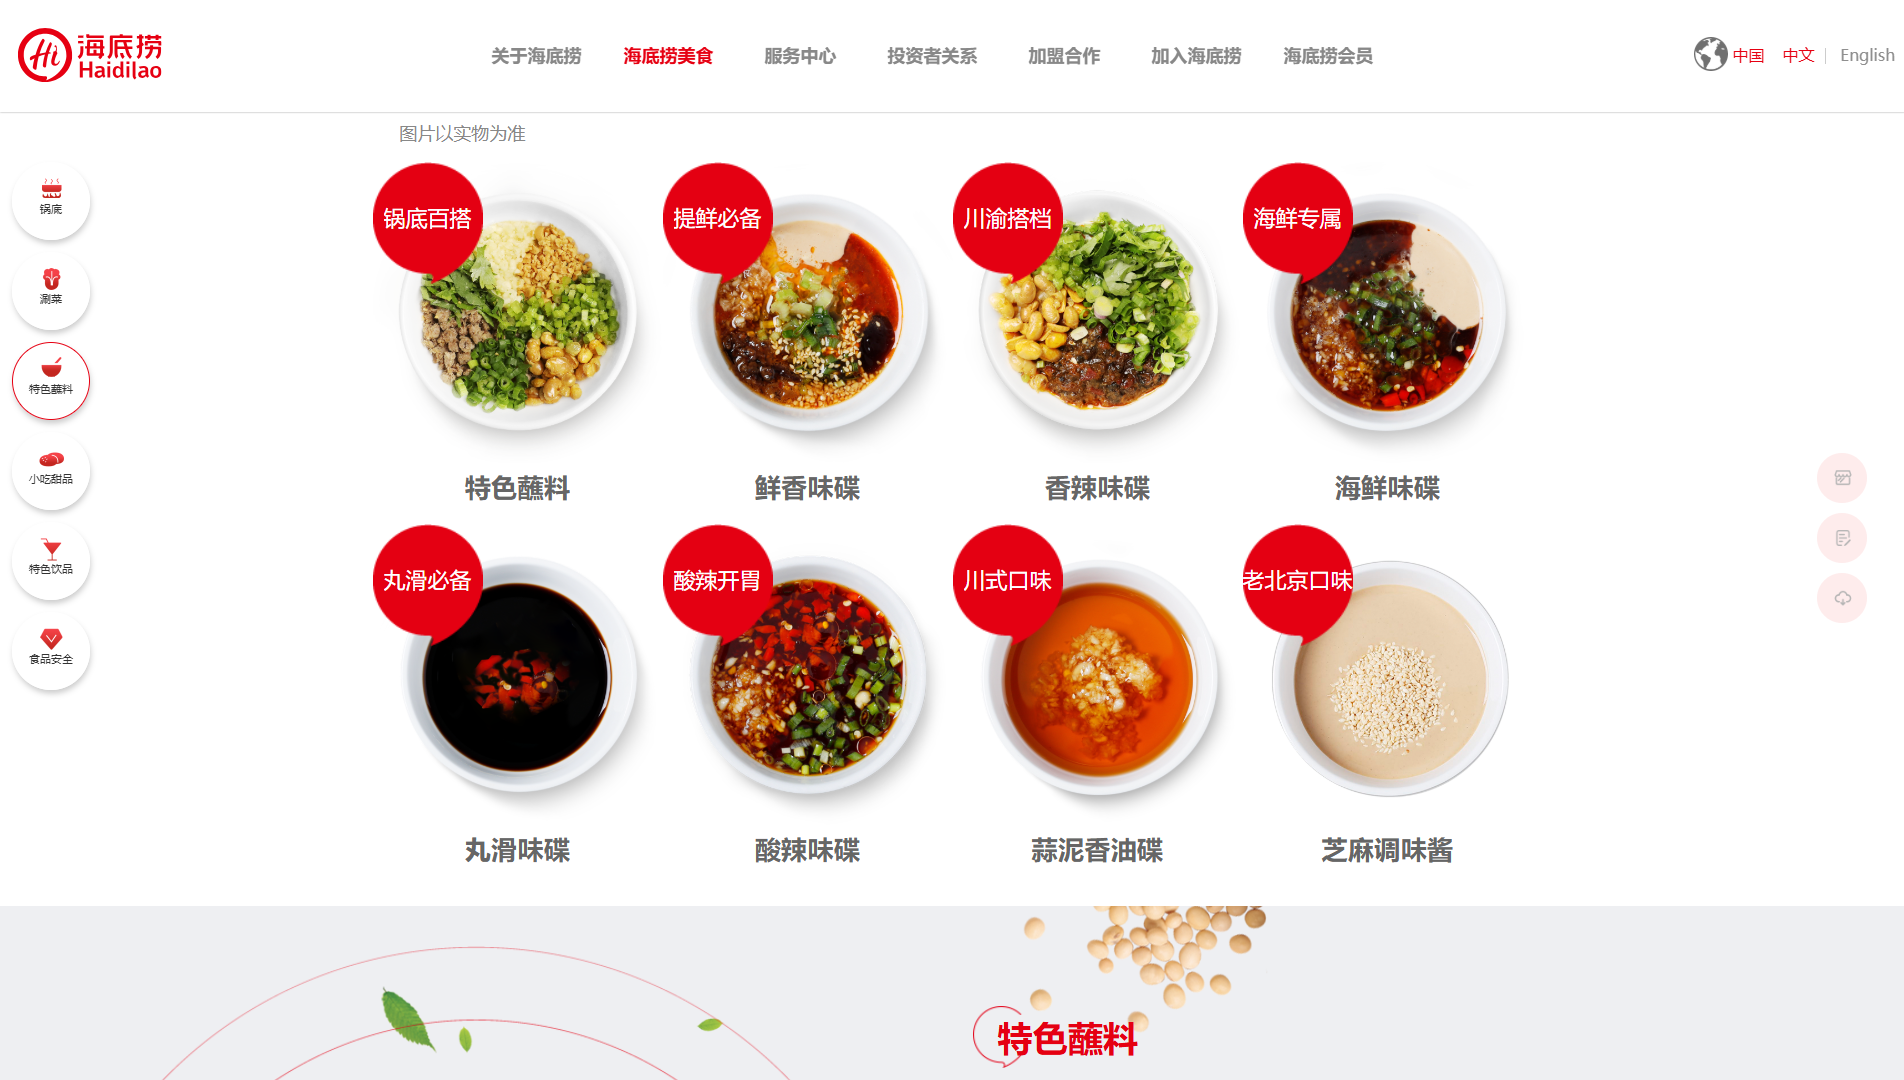
\includegraphics[width=15cm]{Images/haidilao.png}
    \vspace{0.5cm}
    \caption{Giao diện website Haidilao}
    \label{fig:my_label}
\end{figure}

Haidilao là chuỗi nhà hàng lẩu nổi tiếng, thành lập năm 1994 tại Giản Dương, Tứ Xuyên, Trung Quốc. Với dịch vụ khách hàng xuất sắc và hương vị lẩu đặc trưng, Haidilao đã mở rộng ra toàn cầu với hơn 1.300 nhà hàng tại nhiều quốc gia, bao gồm Việt Nam. Trang web chính thức của Haidilao \href{https://www.haidilao.com/}{"https://www.haidilao.com"} cung cấp thông tin về thực đơn, địa điểm các chi nhánh và dịch vụ khách hàng, giúp thực khách dễ dàng tiếp cận và trải nghiệm ẩm thực độc đáo của Haidilao.

\subsection{Yoshinoya}

\begin{figure}[H]
    \centering
    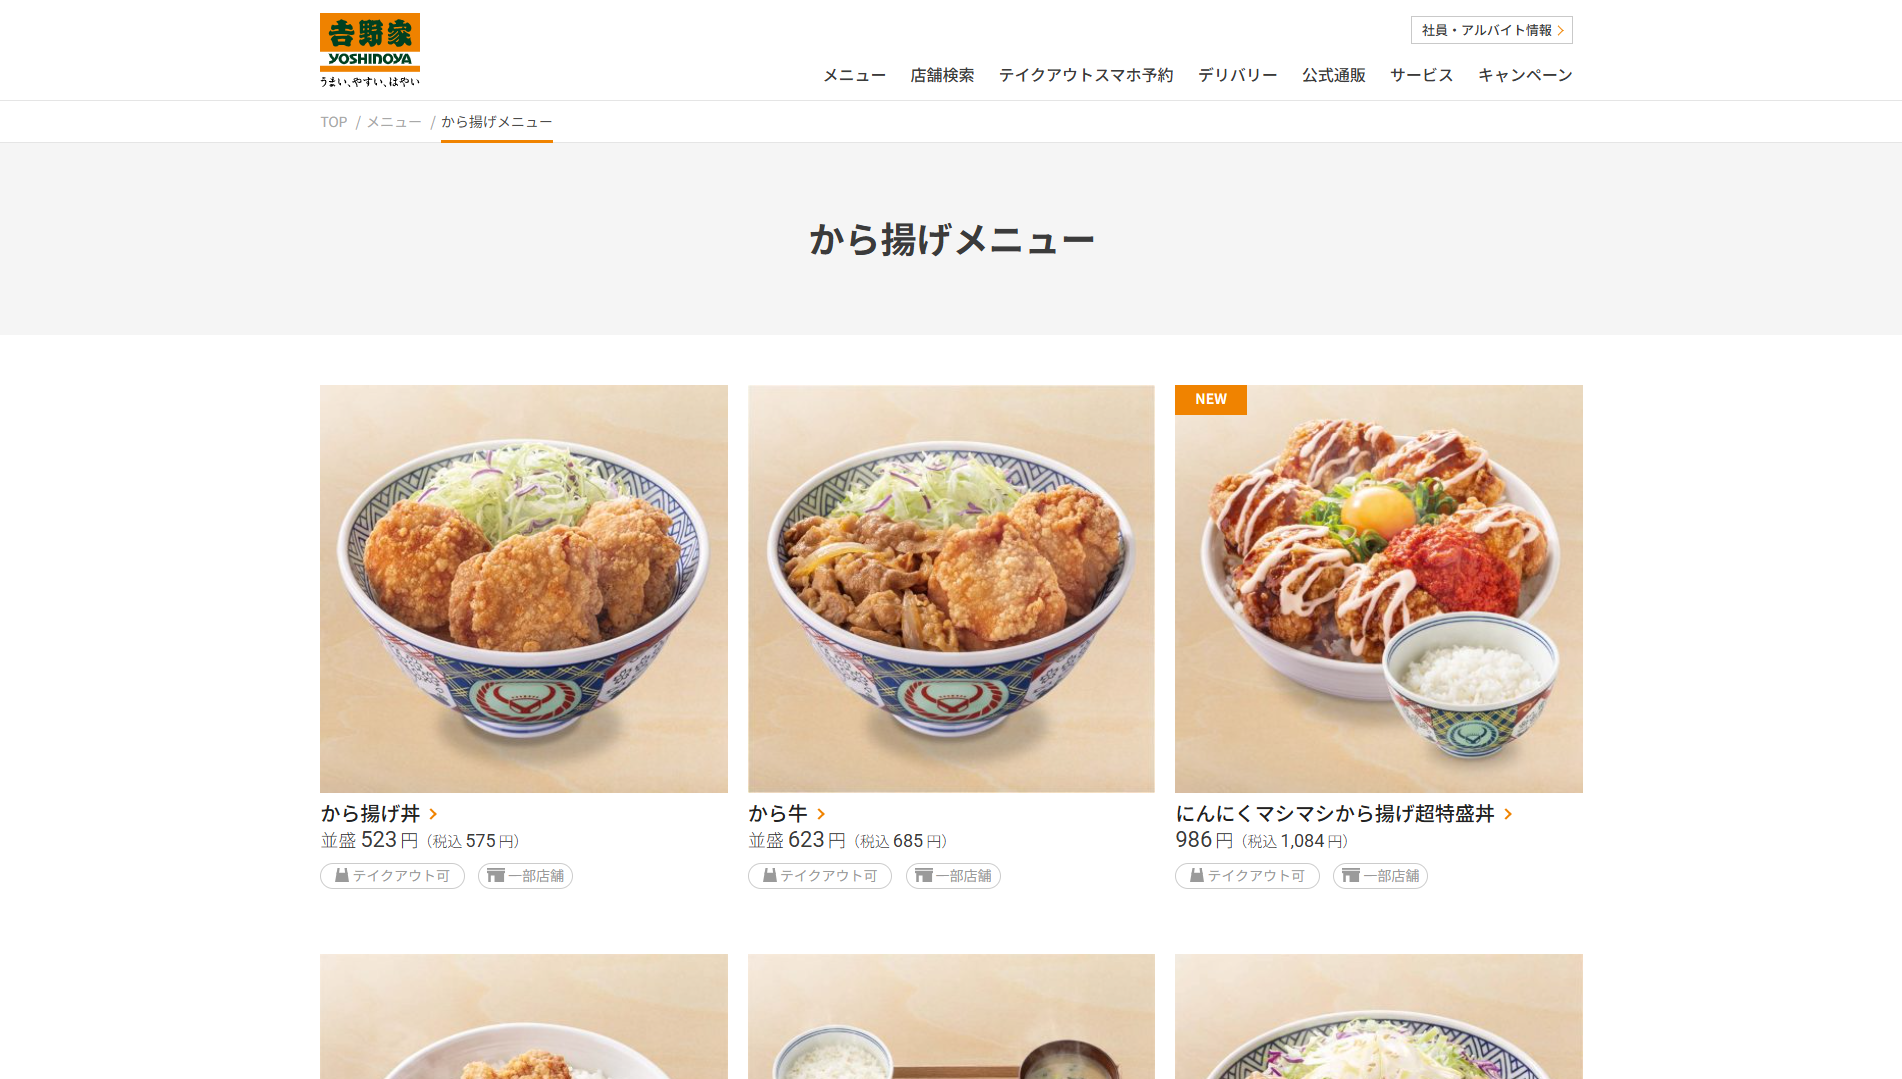
\includegraphics[width=15cm]{Images/yoshinoya.png}
    \vspace{0.5cm}
    \caption{Giao diện website Yoshinoya}
    \label{fig:my_label}
\end{figure}

Yoshinoya là một chuỗi nhà hàng nổi tiếng của Nhật Bản, ra đời từ năm 1899 tại Tokyo, chuyên phục vụ các món ăn truyền thống như gyudon (cơm bò hầm), cơm gà teriyaki và súp miso. Với hơn 120 năm lịch sử, Yoshinoya tự hào mang đến hương vị đậm đà, nguyên liệu tươi ngon và dịch vụ nhanh chóng, tiện lợi. Hiện nay, chuỗi này có mặt tại nhiều quốc gia, trở thành biểu tượng của ẩm thực Nhật Bản đơn giản nhưng tinh tế. Trang web chính thức của Yoshinoya \href{www.yoshinoya.com}{"www.yoshinoya.com"}  giúp khách hàng có thể thưởng thức món ăn yêu thích mọi lúc, mọi nơi thông qua các dịch vụ mà họ cung cấp.

\subsection{Cơm Niêu Sài Gòn}

\begin{figure}[H]
    \centering
    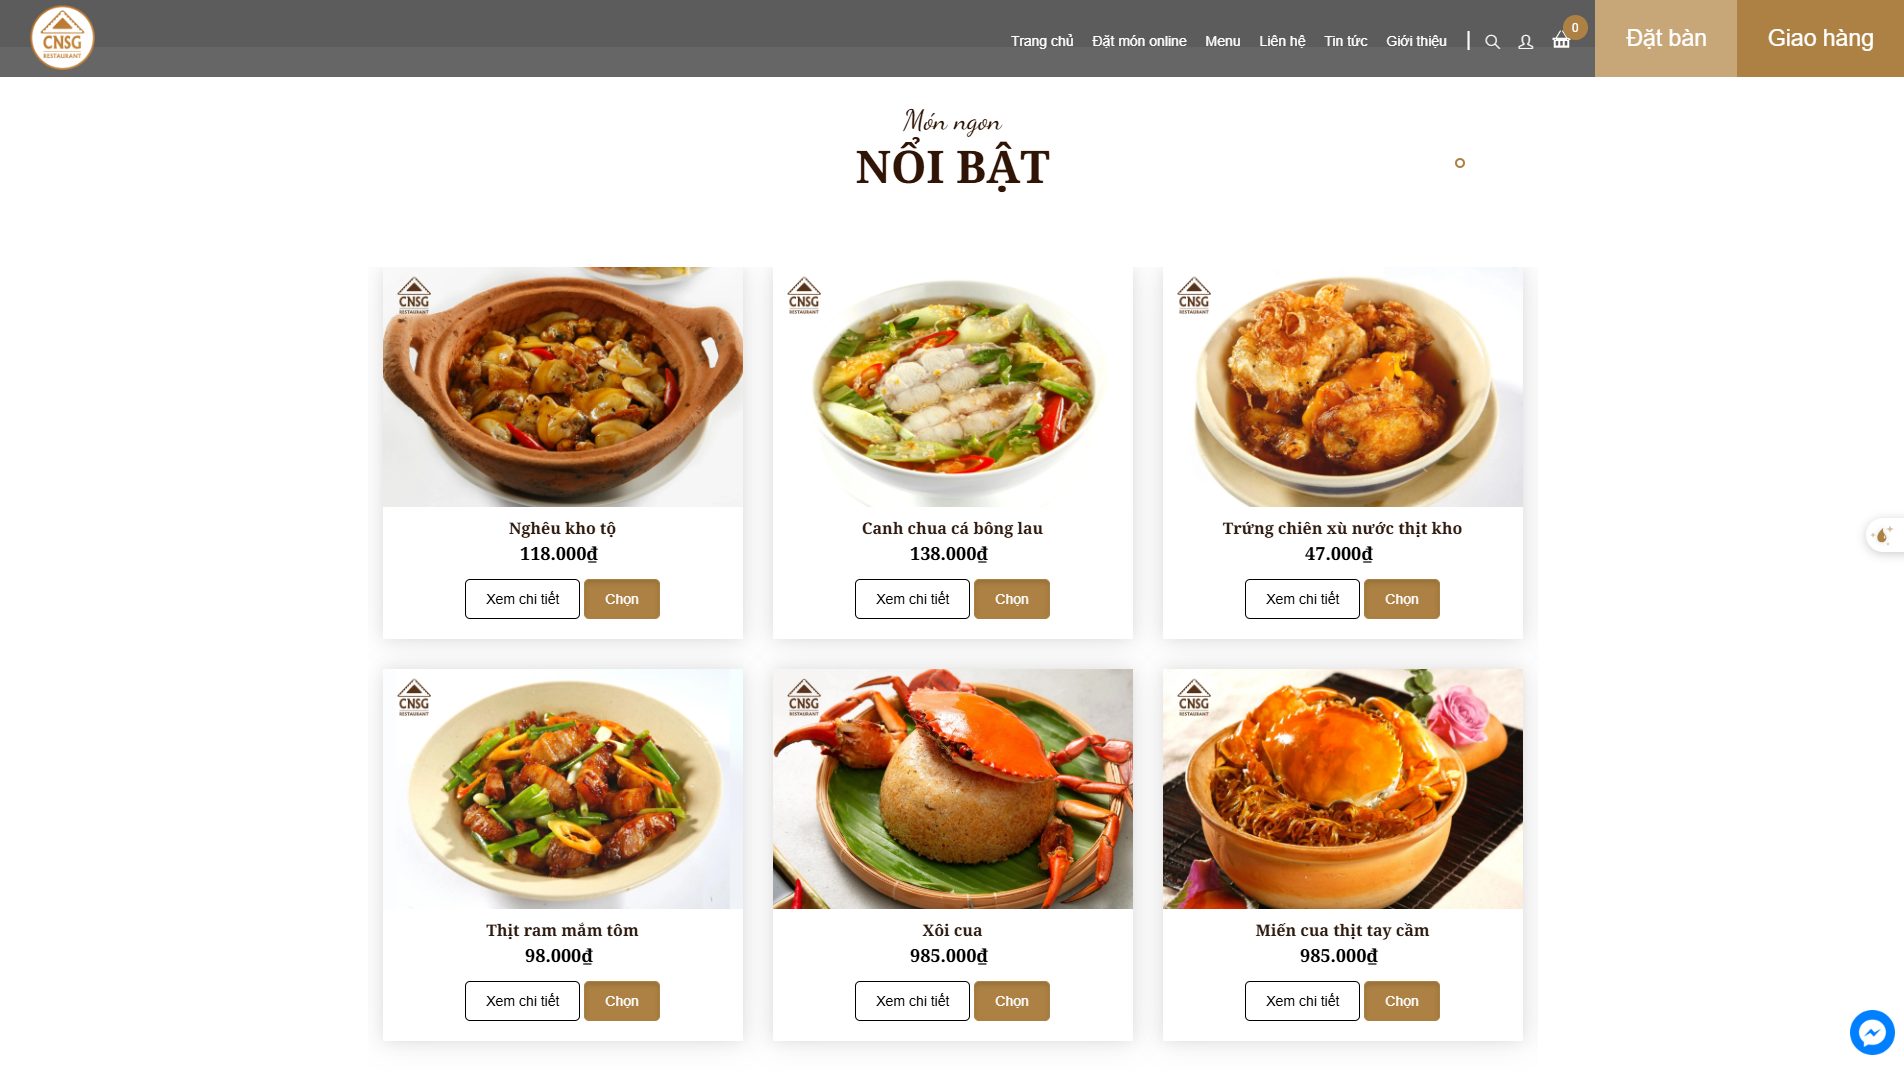
\includegraphics[width=15cm]{Images/comnieusaigon.png}
    \vspace{0.5cm}
    \caption{Giao diện website Cơm niêu Sài Gòn}
    \label{fig:my_label}
\end{figure}

Cơm Niêu Sài Gòn là một địa chỉ ẩm thực truyền thống nổi tiếng qua nhiều thế hệ. Nằm tại quận 3, TP.HCM, nhà hàng thu hút đông đảo khách hàng, đặc biệt là các gia đình và du khách, đến thưởng thức những món ăn đặc sản của miền Nam Việt Nam. Với không gian ấm cúng và thực đơn phong phú, nhà hàng mang đến những bữa ăn đậm đà hương vị quê hương, làm hài lòng cả những thực khách khó tính nhất. Bạn có thể khám phá thêm về thực đơn và dịch vụ của nhà hàng qua trang web chính thức của Cơm Niêu Sài Gòn tại \href{https://comnieusaigon.com}{"https://comnieusaigon.com"}.

\subsection{Thanh's Deli}

\begin{figure}[H]
    \centering
    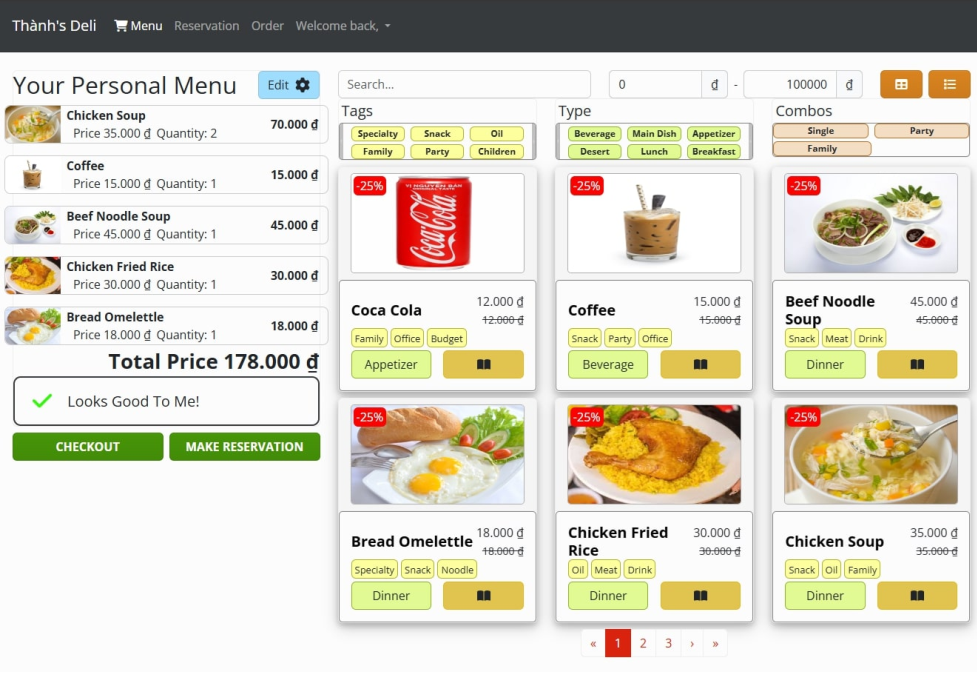
\includegraphics[width=15cm]{Images/thanhsdeli.png}
    \vspace{0.5cm}
    \caption{Giao diện website Thanh's Deli}
    \label{fig:my_label}
\end{figure}

Thanh's Deli là một hệ thống quản lý đặt món và đặt bàn trực tuyến được phát triển bởi Nguyễn Duy Thành trong khuôn khổ đồ án tốt nghiệp. Hệ thống được thiết kế nhằm nâng cao trải nghiệm người dùng tại nhà hàng, giúp khách hàng dễ dàng thực hiện các thao tác đặt món và đặt bàn qua nền tảng trực tuyến.
% % % % % % % 
\subsection{So sánh với hệ thống của nhóm}

Chúng em sẽ tiến hành so sánh hệ thống của mình với các hệ thống khác trong ngành, tập trung vào các chức năng mà họ cung cấp cho khách hàng. Cụ thể, chúng em sẽ đánh giá các nội dung trên trang web của họ, cách thức trình bày các thông tin đó và mức độ tương tác giữa người dùng và hệ thống.

Chúng em sẽ kiểm tra xem các hệ thống có cung cấp 10 nội dung sau đây không: Giới thiệu, Thực đơn, Đặt món trực tuyến, Đặt bàn, Đánh giá và bình luận, Khuyến mãi, Thông tin liên hệ, Đăng nhập/Tài khoản cá nhân, Tương thích di động, và Hỗ trợ khách hàng. Chúng em sẽ đánh giá cách thức trình bày và mức độ hoàn thiện của từng nội dung theo các cấp độ phân loại chi tiết dưới đây:

        \begin{enumerate}
            \item Giới thiệu
                \begin{itemize}
                    \item Cấp độ 1: Cung cấp thông tin cơ bản về nhà hàng (tên, địa chỉ).
                    \item Cấp độ 2: Bao gồm thông tin cơ bản cùng với lịch sử, sứ mệnh và tầm nhìn của nhà hàng.
                    \item Cấp độ 3: Ngoài các thông tin trên, còn có câu chuyện thương hiệu, giới thiệu đội ngũ quản lý và đầu bếp, cùng các giải thưởng đã đạt được.
                \end{itemize}
            \item Thực đơn
                \begin{itemize}
                    \item Cấp độ 1: Danh sách các món ăn và đồ uống cơ bản.
                    \item Cấp độ 2: Thực đơn kèm theo mô tả chi tiết và giá cả cho từng món.
                    \item Cấp độ 3: Thực đơn bao gồm hình ảnh chất lượng cao cho mỗi món, thông tin về nguyên liệu và giá trị dinh dưỡng.
                \end{itemize}
            \item Đặt món trực tuyến
                \begin{itemize}
                    \item Cấp độ 1: Thực đơn sẽ có phần riêng để khách hàng thêm món ăn vào đơn hàng của mình.
                    \item Cấp độ 2: Có hệ thống giỏ hàng cho phép khách hàng có thể coi lại những món ăn trước khi tạo đơn.
                    \item Cấp độ 3: Cho phép thanh toán trực tuyến thông qua các hình thức thanh toán online.
                \end{itemize}
            \item Đặt bàn
                \begin{itemize}
                    \item Cấp độ 1: Cho phép đặt bàn thông qua form cơ bản.
                    \item Cấp độ 2: Hiển thị trạng thái bàn và cập nhật trạng thái theo thời gian thực.
                    \item Cấp độ 3: Cung cấp sơ đồ chi tiết của nhà hàng, cho phép người dùng xem tổng quan các vị trí bàn còn trống.
                \end{itemize}
            \item Đánh giá và bình luận
                \begin{itemize}
                    \item Cấp độ 1: Cho phép nhìn thấy những bình luận do nhà hàng thu thập được, nhưng không cho phép bình luận trực tiếp trên hệ thống.
                    \item Cấp độ 2: Cho phép khách hàng đánh giá, bình luận trực tiếp và nhận phản hồi từ quản lý nhà hàng.
                \end{itemize}
            \item Khuyến mãi
                \begin{itemize}
                    \item Cấp độ 1: Giảm giá cho một món ăn cụ thể với mức giảm cố định.
                    \item Cấp độ 2: Cho phép sử dụng mã giảm giá hoặc voucher.
                    \item Cấp độ 3: Cung cấp chương trình tích điểm dành cho khách hàng thân thiết.
                \end{itemize}
            \item Thông tin liên hệ
                \begin{itemize}
                    \item Cấp độ 1: Chỉ cung cấp địa chỉ và số điện thoại.
                    \item Cấp độ 2: Thêm email liên hệ và bản đồ chỉ đường.
                    \item Cấp độ 3: Có form liên hệ trực tuyến, liên kết với mạng xã hội và hỗ trợ chat trực tiếp.
                \end{itemize}
            \item Đăng nhập/Tài khoản cá nhân
                \begin{itemize}
                    \item Cấp độ 1: Cho phép tạo tài khoản, không dùng mạng xã hôi.
                    \item Cấp độ 2: Cho phép dùng mạng xã hôi để đăng nhập.
                    \item Cấp độ 3: Tài khoản cá nhân cho phép xem lịch sử đặt hàng, nhận ưu đãi dành riêng và quản lý thông tin cá nhân.
                \end{itemize}
            \item Tương thích di động
                \begin{itemize}
                    \item Cấp độ 1: Hiển thị trên di động nhưng chưa tối ưu giao diện và chức năng.
                    \item Cấp độ 2: Tương thích hoàn toàn với thiết bị di động, giao diện và chức năng được tối ưu hóa.
                \end{itemize}
            \item Hỗ trợ khách hàng
                \begin{itemize}
                    \item Cấp độ 1: Cung cấp số điện thoại hỗ trợ chỉ trong giờ hành chính (ví dụ: 8h-17h). Khách hàng có thể gọi khi cần hỗ trợ về các vấn đề cơ bản như đặt món, thắc mắc về dịch vụ.
                    \item Cấp độ 2: Cung cấp email hỗ trợ, khách hàng có thể gửi yêu cầu qua email về các vấn đề cần giải đáp, và nhận phản hồi trong vòng 24 giờ. Hỗ trợ các vấn đề liên quan đến đơn hàng, thanh toán hoặc yêu cầu thông tin thêm về dịch vụ.
                    \item Cấp độ 3: Hỗ trợ khách hàng qua nhiều kênh (chat trực tuyến, email, điện thoại, form liên hệ) với phản hồi nhanh chóng 24/7. Khách hàng có thể liên hệ bất cứ lúc nào để giải quyết các vấn đề khẩn cấp như yêu cầu thay đổi đơn hàng, khiếu nại, hay cần trợ giúp về dịch vụ trong suốt quá trình sử dụng.
                \end{itemize}
        \end{enumerate}

        \begin{longtable}{|p{2cm}|p{1.5cm}|p{1.5cm}|p{1.5cm}|p{1.5cm}|p{1.5cm}|p{1.5cm}|p{1.5cm}|}
        \hline
        \textbf{Chức năng} & \textbf{Menu+ (Our System)} & \textbf{Cracco} & \textbf{KFC} & \textbf{Haidilao} & \textbf{Yoshinoya} & \textbf{Cơm Niêu Sài Gòn} & \textbf{Thanh's Deli}\\ 
        \hline
        \endfirsthead
        \hline
        \textbf{Chức năng} & \textbf{Menu+ (Our System)} & \textbf{Cracco} & \textbf{KFC} & \textbf{Haidilao} & \textbf{Yoshinoya} & \textbf{Cơm Niêu Sài Gòn} & \textbf{Thanh's Deli} \\
        \endhead
        \hline
        % \multicolumn{8}{|r|}{\small\slshape Còn tiếp} \\ \hline
        \endfoot
        \hline
        \endlastfoot
        Giới thiệu & 3 & 2 & 3 & 3 & 3 & 3 & 3\\ 
        \hline
        Thực đơn & 3 & 2 & 3 & 2 & 3 & 2 & 2\\ 
        \hline
        Đặt món trực tuyến & 3 & 0 & 3 & 3 & 3 & 3 & 3\\ 
        \hline
        Đặt bàn & 3 & 1 & 1 & 1 & 2 & 1 & 3\\ 
        \hline
        Đánh giá và bình luận & 2 & 0 & 0 & 0 & 2 & 0 & 2\\ 
        \hline
        Khuyến mãi & 2 & 2 & 3 & 3 & 2 & 2 & 2\\ 
        \hline
        Thông tin liên hệ & 3 & 1 & 3 & 2 & 3 & 3 & 2\\ 
        \hline
        Đăng nhập/Tài khoản cá nhân & 3 & 3 & 3 & 3 & 1 & 3 & 1\\ 
        \hline
        Tương thích di động & 2 & 2 & 2 & 2 & 2 & 2 & 2\\ 
        \hline
        Hỗ trợ khách hàng & 2 & 2 & 3 & 2 & 1 & 2 & 2\\ 
        \hline
        \caption{Bảng so sánh các nhà hàng}\\
        \end{longtable}

\subsection{Kết luận}
Việc so sánh hệ thống của nhóm với các hệ thống hiện có trong ngành nhà hàng đã giúp làm rõ những ưu điểm và nhược điểm của sản phẩm mà nhóm phát triển. Hệ thống của nhóm nổi bật với một số điểm mạnh quan trọng khi so sánh với các hệ thống liên quan.

Đầu tiên, hệ thống của chúng em được cải tiến với khả năng tích hợp các tính năng như tự gọi món qua ứng dụng và thanh toán trực tuyến. Mặc dù các hệ thống như Cơm Niêu Sài Gòn, KFC và Haidilao cũng đã triển khai các tính năng đặt món trực tuyến và thanh toán, nhưng hệ thống của nhóm mang đến một trải nghiệm người dùng dễ dàng và nhanh chóng hơn nhờ vào giao diện thân thiện và tiện lợi. Hơn nữa, hệ thống của nhóm cung cấp phản hồi thời gian thực và khả năng theo dõi đơn hàng một cách thuận tiện, điều mà một số hệ thống khác còn thiếu sót.

Mặc dù hệ thống của chúng em có những ưu điểm về việc tối ưu trải nghiệm người dùng và quy trình, song so với các hệ thống như Yoshinoya hay KFC, hệ thống của nhóm vẫn còn hạn chế về tính linh hoạt trong việc mở rộng các tính năng phức tạp hơn, như tích hợp chương trình khách hàng thân thiết hay quản lý các chương trình khuyến mãi phức tạp. Các tính năng như phân tích hành vi mua sắm và khuyến mãi dựa trên tần suất vẫn là những lĩnh vực cần cải tiến.

Tóm lại, hệ thống của chúng em thể hiện sự vượt trội trong việc tối ưu hóa quy trình đặt món và thanh toán, giúp nâng cao hiệu quả công việc và cải thiện trải nghiệm khách hàng. Tuy nhiên, để có thể phát triển mạnh mẽ hơn, hệ thống cần học hỏi và cải tiến thêm ở những lĩnh vực mở rộng tính năng và quản lý khách hàng. Việc so sánh này đã giúp nhóm nhận diện rõ các điểm mạnh hiện tại cũng như những khu vực cần cải thiện, làm cơ sở để phát triển hệ thống trong tương lai.







% \newpage
% \section{TỔNG QUAN VỀ HỆ THỐNG}

\subsection{Bối cảnh kinh doanh (Business context)}
Trong bối cảnh ngành công nghiệp thực phẩm và dịch vụ ngày càng phát triển và cạnh tranh khốc liệt, việc ứng dụng công nghệ vào quản lý nhà hàng đã trở thành một xu hướng tất yếu. Hệ thống quản lý chuỗi nhà hàng là một giải pháp kỹ thuật số được thiết kế để hỗ trợ và tối ưu hóa các hoạt động vận hành hàng ngày của nhà hàng (đặc biệt là nhà hàng fine dining), từ đặt bàn, xử lý đơn hàng, thanh toán cho đến quản lý nhân sự. Một hệ thống quản lý chuỗi nhà hàng hiệu quả không chỉ giúp nâng cao trải nghiệm của khách hàng mà còn cải thiện hiệu suất làm việc của nhân viên và tối ưu hóa quản lý doanh thu.

% \subsubsection{Mục tiêu và phạm vi hệ thống}
% Hệ thống quản lý nhà hàng \textbf{\textit{Menu+}} được phát triển nhằm mục đích đơn giản hóa và nâng cao hiệu quả các hoạt động vận hành hàng ngày trong một nhà hàng fine dining. Các chức năng chính của \textbf{\textit{Menu+}} bao gồm:
% \begin{itemize}
%     \item \textbf{Đặt bàn trực tuyến và quản lý bàn}: Giúp khách hàng dễ dàng đặt chỗ và hỗ trợ nhân viên theo dõi trạng thái bàn một cách chính xác.
%      \item \textbf{Quản lý bàn}: Hỗ trợ nhân viên theo dõi trạng thái bàn (trống, đã đặt, đang phục vụ) và thực hiện các thao tác như chuyển bàn khi cần thiết.
%     \item \textbf{Xử lý đơn hàng}: Cho phép nhân viên nhập đơn hàng, tùy chỉnh theo yêu cầu của khách và gửi trực tiếp đến hệ thống hiển thị bếp (Kitchen Display System - KDS).
%     \item \textbf{Thanh toán và quản lý doanh thu}: Tích hợp các phương thức thanh toán đa dạng, tạo điều kiện thuận lợi cho cả khách hàng và nhà hàng.
%     \item \textbf{Quản lý quan hệ khách hàng (CRM) và nhân sự}: Lưu trữ thông tin khách hàng, quản lý lịch làm việc của nhân viên và cung cấp các báo cáo chi tiết về hoạt động kinh doanh.
% \end{itemize}
% \textbf{\textit{Menu+}} linh hoạt và thân thiện với người dùng đóng vai trò quan trọng trong việc giúp các nhà hàng, đặc biệt là những nhà hàng mới khởi nghiệp, mở rộng quy mô hoạt động một cách hiệu quả.

% \subsubsection{Ràng buộc kinh doanh (Business Constraint)}

% exclude

\subsubsection{Tổng quan hệ thống quản lý nhà hàng}

Dưới đây là mô tả tổng quan về các thành phần cấu thành hệ thống quản lý chuỗi nhà hàng, với các chức năng thiết yếu nhằm hỗ trợ việc vận hành và điều phối các hoạt động trong một chuỗi nhà hàng hiện đại. Những hệ thống con này đóng vai trò quan trọng trong việc tối ưu hóa hiệu quả công việc, nâng cao chất lượng dịch vụ và đảm bảo sự hoạt động trơn tru của toàn bộ chuỗi.

\begin{figure}[H]
	\centering
	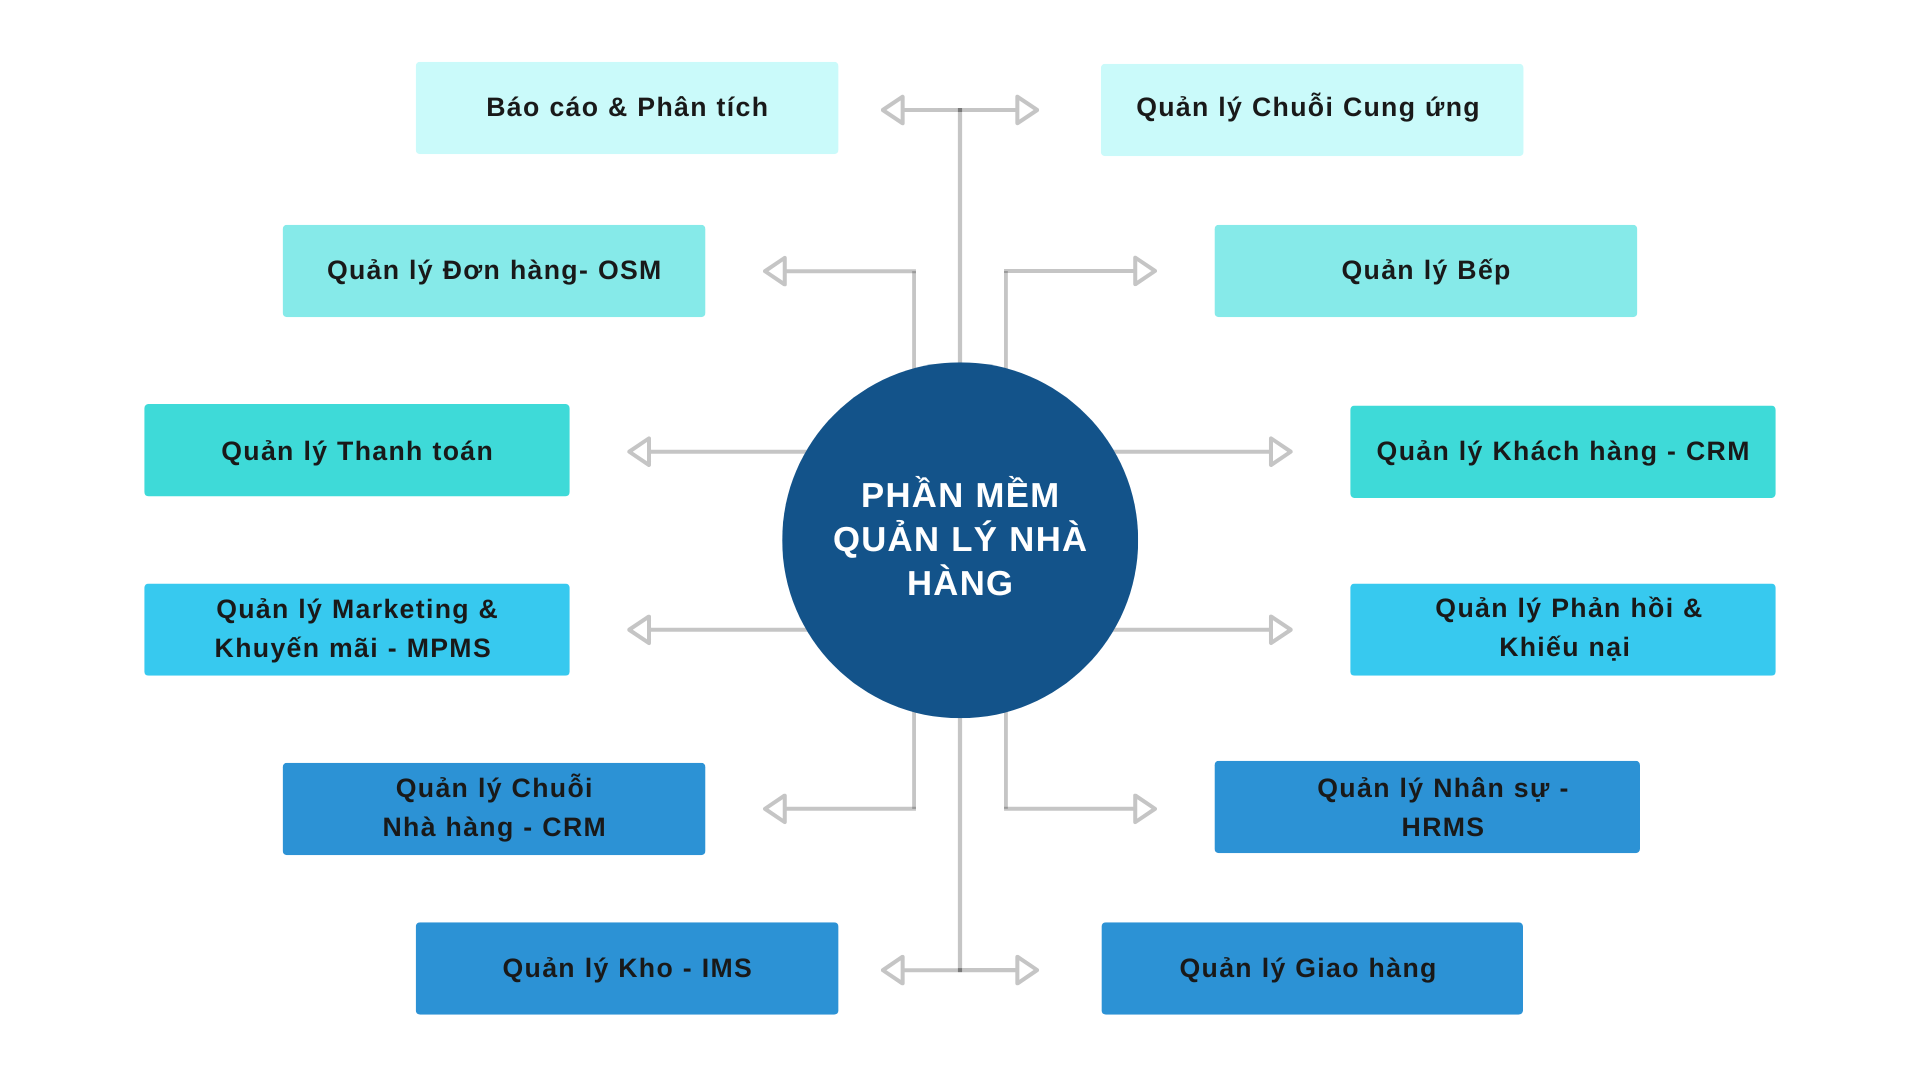
\includegraphics[width=15cm]{Images/so-do-he-thong.png}
	\vspace{0.5cm}
	\caption{Sơ đồ tổng quan về một hệ thống Quản lý Nhà hàng}
	\label{fig:my_label}
\end{figure}

\begin{itemize}
	\item \textbf{Hệ thống Quản lý Đơn hàng (Order Management System - OMS)}: Đóng vai trò quan trọng trong việc tiếp nhận và xử lý các đơn đặt món từ khách hàng. Khi khách hàng đặt món, thông tin đơn hàng sẽ được hệ thống OMS ghi nhận và phân phối đến các bộ phận liên quan trong nhà hàng, như bếp để chế biến món ăn, thu ngân để xử lý thanh toán, và đội ngũ giao hàng nếu có. Hệ thống OMS không chỉ giúp theo dõi tình trạng của từng đơn hàng mà còn quản lý các thông tin liên quan đến khách hàng và việc giao nhận món ăn. Đặc biệt, OMS sẽ giúp nhà quản lý theo dõi hiệu suất của đơn hàng và cập nhật kịp thời trạng thái để khách hàng có thể nhận được món ăn một cách nhanh chóng. Mọi thay đổi về đơn hàng sẽ được cập nhật liên tục để các bộ phận liên quan có thể xử lý ngay khi có sự thay đổi, ví dụ như khi khách hàng hủy đơn hoặc có yêu cầu thay đổi món.

	\item \textbf{Hệ thống Quản lý Bếp (Kitchen Management System - KMS)}: Tập trung vào việc quản lý quá trình chế biến món ăn từ khi nhận được đơn hàng từ OMS cho đến khi món ăn hoàn thành và sẵn sàng phục vụ khách. Thông qua KMS, nhà bếp có thể lên kế hoạch chế biến cho từng món ăn và theo dõi hiệu quả làm việc của từng đầu bếp. Mỗi đơn hàng sẽ được chia thành các công đoạn nhỏ để các nhân viên bếp dễ dàng theo dõi và thực hiện. Hệ thống này cũng đóng vai trò trong việc quản lý chất lượng món ăn, đảm bảo rằng món ăn được chế biến đúng quy trình và đạt tiêu chuẩn chất lượng. KMS cũng kết nối với các hệ thống khác như Inventory Management System (IMS) để tự động kiểm tra và yêu cầu bổ sung nguyên liệu khi kho hàng thiếu hụt.

	\item \textbf{Hệ thống Quản lý Kho (Inventory Management System - IMS)}: Quản lý và giám sát tình trạng nguyên liệu trong kho của các chi nhánh nhà hàng. IMS giúp nhà quản lý kiểm soát số lượng nguyên liệu, hạn sử dụng và các mặt hàng còn lại trong kho để đảm bảo rằng luôn có đủ nguyên liệu cho việc chế biến món ăn. Hệ thống này sẽ tự động thông báo khi lượng nguyên liệu sắp hết hoặc sắp hết hạn sử dụng, giúp bộ phận kho có thể lên kế hoạch nhập hàng bổ sung từ các nhà cung cấp. IMS không chỉ giúp đảm bảo việc cung cấp nguyên liệu kịp thời cho KMS, mà còn giúp giảm thiểu tình trạng thiếu hụt nguyên liệu, qua đó đảm bảo việc phục vụ khách hàng không bị gián đoạn. Hệ thống này cũng giúp tối ưu hóa việc sử dụng nguyên liệu, giảm lãng phí và giúp duy trì chi phí vận hành hợp lý.

	\item \textbf{Hệ thống Quản lý Thanh toán (Payment Management System - PMS)}: Chịu trách nhiệm xử lý tất cả các giao dịch thanh toán của khách hàng sau khi món ăn được giao đến bàn hoặc giao tận nơi. Khi món ăn hoàn thành và khách hàng chuẩn bị thanh toán, hệ thống PMS sẽ tự động tính toán giá trị đơn hàng, bao gồm thuế, chiết khấu, và các khoản phí khác nếu có. Hệ thống này hỗ trợ nhiều phương thức thanh toán khác nhau, từ tiền mặt, thẻ tín dụng, thẻ ghi nợ, cho đến các phương thức thanh toán trực tuyến. Sau khi thanh toán hoàn tất, PMS sẽ in hóa đơn cho khách và cập nhật dữ liệu doanh thu vào hệ thống tài chính. Hệ thống này cũng đồng bộ hóa dữ liệu với các hệ thống báo cáo để nhà quản lý có cái nhìn tổng quan về tình hình tài chính của từng chi nhánh. PMS còn có khả năng theo dõi và phân tích các xu hướng chi tiêu của khách hàng để đưa ra các chiến lược giá hợp lý và tăng trưởng doanh thu.

	\item \textbf{Hệ thống Quản lý Nhân sự (Human Resource Management System - HRMS)}: Quản lý thông tin nhân viên, lịch làm việc và hiệu suất công việc của các nhân viên trong chuỗi nhà hàng. Hệ thống này theo dõi số giờ làm việc, ca làm việc của nhân viên, và các yếu tố liên quan đến chấm công, bảo hiểm, tiền lương. Ngoài ra, HRMS còn hỗ trợ việc phân công công việc cho các nhân viên bếp, thu ngân, và các bộ phận khác, giúp việc tổ chức công việc trở nên khoa học và hợp lý. Các tính năng như theo dõi kỳ nghỉ, đào tạo và phát triển nhân viên cũng được HRMS đảm bảo. Một trong những chức năng quan trọng của HRMS là giúp tối ưu hóa quy trình tuyển dụng, giúp tuyển chọn nhân viên phù hợp với yêu cầu công việc. Ngoài ra, HRMS còn hỗ trợ các bộ phận quản lý nhân sự của từng chi nhánh trong việc đánh giá hiệu suất làm việc và cải thiện chất lượng nhân sự.

	\item \textbf{Hệ thống Báo cáo \& Phân tích (Reporting \& Analytics System - R\&A)}: Quản lý có cái nhìn tổng quan về hiệu suất của toàn chuỗi nhà hàng. Hệ thống này thu thập và tổng hợp dữ liệu từ các hệ thống khác nhau như OMS, KMS, IMS, PMS và HRMS để tạo ra các báo cáo chi tiết. Những báo cáo này không chỉ về tình hình doanh thu, mà còn cung cấp các thông tin liên quan đến hiệu quả công việc của nhân viên, tình trạng kho nguyên liệu, mức độ hài lòng của khách hàng, và nhiều yếu tố khác. Thông qua phân tích dữ liệu, nhà quản lý có thể đưa ra những quyết định chiến lược giúp cải thiện quy trình hoạt động, tối ưu hóa chi phí và nâng cao chất lượng dịch vụ. Hệ thống cũng hỗ trợ tạo ra các báo cáo tài chính, giúp các chi nhánh có thể theo dõi doanh thu và chi phí một cách chi tiết.

	\item \textbf{Hệ thống Quản lý Chuỗi Cung ứng (Supply Chain Management System - SCM)}: Quản lý và điều phối mối quan hệ với các nhà cung cấp, đảm bảo nguồn nguyên liệu luôn được cung cấp đầy đủ và đúng chất lượng. SCM theo dõi tình trạng đơn hàng từ khi nguyên liệu được đặt hàng cho đến khi nhận được hàng và đưa vào kho. Hệ thống này không chỉ giúp kiểm soát chất lượng nguồn cung mà còn tối ưu hóa quá trình giao nhận nguyên liệu, giảm thiểu tình trạng thiếu hụt hoặc tồn đọng hàng hóa trong kho. Bằng cách kết hợp dữ liệu từ IMS và KMS, SCM có thể dự báo nhu cầu nguyên liệu cho các món ăn, từ đó có kế hoạch đặt hàng hiệu quả hơn.

	\item \textbf{Hệ thống Quản lý Khách hàng (Customer Relationship Management - CRM)}: Lưu trữ và quản lý thông tin của khách hàng, bao gồm các thông tin cá nhân, lịch sử đơn hàng và các thói quen tiêu dùng. Hệ thống CRM giúp nhà hàng không chỉ lưu giữ thông tin khách hàng mà còn tạo dựng mối quan hệ lâu dài với khách hàng thông qua các chương trình khách hàng thân thiết và các ưu đãi cá nhân hóa. Bằng cách phân tích dữ liệu từ CRM, nhà hàng có thể hiểu rõ hơn về nhu cầu và sở thích của khách hàng, từ đó đề xuất các món ăn phù hợp, tạo ra những trải nghiệm cá nhân hóa. Hệ thống này còn hỗ trợ việc gửi các thông báo về chương trình khuyến mãi, sự kiện đặc biệt, hoặc thông tin về các sản phẩm mới đến khách hàng, giúp duy trì và phát triển mối quan hệ với khách hàng cũ và thu hút khách hàng mới.

	\item \textbf{Hệ thống Quản lý Marketing \& Khuyến mãi (Marketing \& Promotion Management System)}: Lên kế hoạch, triển khai và theo dõi các chiến dịch marketing và chương trình khuyến mãi. Hệ thống này hỗ trợ việc tạo ra các chiến dịch quảng bá các món ăn, khuyến mãi theo mùa hoặc các chương trình giảm giá đặc biệt cho khách hàng. Marketing \& Promotion Management System cung cấp các công cụ để tạo mã giảm giá, quản lý các chương trình khuyến mãi và theo dõi hiệu quả của từng chiến dịch. Hệ thống này còn giúp phân tích dữ liệu khách hàng từ CRM, từ đó xác định đối tượng mục tiêu cho các chiến dịch marketing, giúp tăng tỷ lệ chuyển đổi và tối ưu hóa chi phí marketing. Ngoài ra, các chiến dịch và khuyến mãi cũng có thể được tích hợp với hệ thống thanh toán để khách hàng có thể dễ dàng sử dụng các ưu đãi khi thanh toán.

	\item \textbf{Hệ thống Quản lý Phản hồi \& Khiếu nại (Feedback \& Complaint Management System)}: Nhận và xử lý các phản hồi, khiếu nại từ khách hàng. Việc lắng nghe và giải quyết nhanh chóng các vấn đề của khách hàng giúp nhà hàng cải thiện chất lượng dịch vụ và tạo dựng lòng tin của khách hàng. Hệ thống này giúp theo dõi các khiếu nại về món ăn, thái độ phục vụ, không gian nhà hàng hoặc các vấn đề khác. Sau khi nhận được phản hồi hoặc khiếu nại từ khách hàng, hệ thống sẽ tự động phân loại và chuyển đến các bộ phận liên quan để xử lý, từ đó giúp khách hàng cảm thấy hài lòng hơn với dịch vụ của nhà hàng. Hệ thống này cũng có chức năng theo dõi các phản hồi tích cực để có thể ghi nhận và thưởng cho những nhân viên hoặc bộ phận có đóng góp xuất sắc.

	\item \textbf{Hệ thống Quản lý Chuỗi Nhà hàng (Chain Management System - CMS)}: Trung tâm quản lý tổng thể của chuỗi các chi nhánh nhà hàng. Hệ thống này giúp giám sát các hoạt động của tất cả các chi nhánh từ một hệ thống tập trung, bao gồm việc theo dõi doanh thu, tồn kho, nhân sự, cũng như các hoạt động vận hành khác của từng chi nhánh. CMS không chỉ giúp đồng bộ hóa các quy trình giữa các chi nhánh mà còn cung cấp các báo cáo tài chính và hoạt động chi tiết để hỗ trợ các quyết định quản lý chiến lược. Hệ thống này tích hợp dữ liệu từ các hệ thống khác như PMS, KMS, IMS, giúp nhà quản lý chuỗi có thể theo dõi tình trạng của từng chi nhánh và đưa ra các quyết định kịp thời để tối ưu hóa hoạt động của toàn chuỗi.

	\item \textbf{Hệ thống Quản lý Giao hàng (Delivery Management System)}: Quản lý các đơn hàng giao tận nơi, bao gồm việc điều phối các nhân viên giao hàng, theo dõi tình trạng đơn hàng và tối ưu hóa thời gian giao hàng. Hệ thống này giúp các nhân viên giao hàng nhận được thông tin đơn hàng một cách nhanh chóng, biết rõ địa chỉ giao hàng và các yêu cầu đặc biệt của khách hàng (nếu có). Hệ thống còn giúp theo dõi trạng thái của đơn hàng từ khi rời khỏi nhà hàng cho đến khi giao đến tay khách hàng, đồng thời cung cấp các công cụ để quản lý các tuyến đường giao hàng sao cho hiệu quả và tiết kiệm thời gian. Việc tích hợp hệ thống này với OMS giúp cập nhật trạng thái của đơn hàng cho khách hàng trong thời gian thực và đảm bảo dịch vụ giao hàng nhanh chóng, chính xác.
\end{itemize}

\subsubsection{Chính sách vận hành (Policy)}
Các nhà hàng hiện đại ngày nay thường áp dụng nhiều chính sách linh hoạt nhằm nâng cao chất lượng phục vụ và giảm thiểu các rủi ro trong kinh doanh. Các chính sách phổ biến được áp dụng có thể kể tới như sau:

\begin{itemize}
	\item \textbf{Đa dạng hóa phương thức thanh toán}: Chính sách này tập trung vào việc cung cấp đa dạng các hình thức thanh toán, như tiền mặt, thẻ tín dụng, ví điện tử và mã QR. Bên cạnh đó, các nhà hàng cũng triển khai hệ thống quản lý thanh toán tự động để rút ngắn thời gian xử lý, giảm thiểu sai sót và tăng trải nghiệm hài lòng của khách hàng. Chính sách này đã được các nhà hàng như \textit{Ngưu Phồn} và \textit{Cơm niêu Sài Gòn} áp dụng rất hiệu quả.

	\item \textbf{Yêu cầu đặt cọc khi đặt bàn}: Để giảm thiểu tổn thất khi khách hàng hủy đặt bàn vào phút chót hoặc không đến nhà hàng mà không báo trước, nhiều nhà hàng áp dụng chính sách yêu cầu khách hàng đặt cọc trước một khoản tiền nhất định, thường dao động từ 10\% đến 20\% tổng giá trị bàn tiệc. Khoản đặt cọc này sẽ được khấu trừ vào hóa đơn thanh toán hoặc bị giữ lại nếu khách hủy đặt bàn trễ hơn thời gian quy định. Một số nhà hàng áp dụng thành công chính sách này là \textit{Nhà Hàng Phúc Thành} và \textit{Vân Nghĩa Palace}.

	\item \textbf{Xác nhận đặt bàn trước ngày hẹn}: Chính sách này yêu cầu nhân viên nhà hàng chủ động liên hệ với khách hàng trước ngày đặt bàn để xác nhận lại thông tin và nhắc nhở khách đến đúng giờ. Điều này không chỉ giúp giảm tình trạng khách quên hay thay đổi kế hoạch mà không thông báo, mà còn giúp nhà hàng quản lý hiệu quả hơn trong việc chuẩn bị dịch vụ. Nhà hàng áp dụng tiêu biểu chính sách này là \textit{Nhà Hàng Phúc Thành}.

	\item \textbf{Chính sách hủy đặt bàn và hoàn tiền rõ ràng}: Các nhà hàng thường đưa ra quy định chi tiết về thời hạn hủy đặt bàn và mức phí áp dụng khi hủy. Điều này giúp khách hàng hiểu rõ trách nhiệm và quyền lợi của mình khi sử dụng dịch vụ, đồng thời tạo ra sự minh bạch và uy tín trong hoạt động kinh doanh. Chính sách này được áp dụng rõ ràng tại \textit{Nhà Hàng Ocean Bay Vũng Tàu}.

	\item \textbf{Điều kiện hủy đơn hàng}: Chính sách này quy định rõ ràng các điều kiện và thời điểm cụ thể khách hàng được phép hủy đơn hàng, thường là trước khi nhà hàng xác nhận và bắt đầu chuẩn bị món ăn. Điều này giúp nhà hàng giảm thiểu tổn thất về nguyên vật liệu và công sức chế biến không cần thiết. Một ví dụ cụ thể về chính sách này là tại nhà hàng \textit{Patyko}.

	\item \textbf{Phí hủy đơn hàng}: Để bảo vệ quyền lợi và giảm thiểu thiệt hại khi khách hàng hủy đơn sau khi nhà hàng đã bắt đầu chế biến, nhiều nhà hàng đặt ra quy định thu phí hủy hoặc không hoàn lại tiền đặt cọc trong một số trường hợp nhất định. Chính sách này nhằm bù đắp một phần chi phí nguyên vật liệu và nhân công đã bỏ ra. Điển hình trong việc áp dụng chính sách này là \textit{Nhà Hàng Khoái}.

	\item \textbf{Chính sách đổi trả sản phẩm}: Để đảm bảo quyền lợi khách hàng và duy trì chất lượng dịch vụ, các nhà hàng thường áp dụng chính sách đổi trả rõ ràng. Khách hàng được quyền đổi hoặc trả lại món ăn trong các trường hợp món bị lỗi, hỏng, không thể sử dụng hoặc không đảm bảo vệ sinh an toàn thực phẩm. Chính sách này giúp tạo dựng lòng tin và gia tăng uy tín của nhà hàng. Một số nhà hàng nổi bật áp dụng thành công chính sách này là \textit{Sườn Mười} và \textit{Nhà Hàng Khoái}.

\end{itemize}



\begin{table}[H]
	\centering
	\caption{Tổng hợp các chính sách, mô tả và tham khảo từ các nhà hàng hoặc hệ thống liên quan}
	\begin{tabular}{|p{4cm}|p{8cm}|p{4cm}|}
		\hline
		\textbf{Tên chính sách}             & \textbf{Mô tả}                                                                                                                                                                                       & \textbf{Nhà hàng áp dụng}             \\
		\hline
		Đa dạng hóa phương thức thanh toán  & Cung cấp nhiều phương thức thanh toán như tiền mặt, thẻ tín dụng, ví điện tử và mã QR, đồng thời áp dụng hệ thống quản lý thanh toán tự động để giảm thiểu sai sót và tăng tốc độ phục vụ.           & Ngưu Phồn, Cơm niêu Sài Gòn           \\
		\hline
		Yêu cầu đặt cọc khi đặt bàn         & Để giảm thiểu tình trạng khách hàng hủy bàn vào phút chót hoặc không đến mà không báo trước, nhiều nhà hàng yêu cầu khách đặt cọc trước một khoản tiền, thường khoảng 10-20\% tổng giá trị bàn tiệc. & Nhà Hàng Phúc Thành, Vân Nghĩa Palace \\
		\hline
		Xác nhận đặt bàn trước ngày hẹn     & Trước ngày đặt bàn, nhân viên nhà hàng nên gọi điện hoặc nhắn tin xác nhận lại với khách hàng để nhắc nhở và đảm bảo họ sẽ đến.                                                                      & Nhà Hàng Phúc Thành                   \\
		\hline
		Chính sách hủy và hoàn tiền rõ ràng & Nhà hàng cần quy định rõ ràng về thời hạn hủy đặt bàn và mức phí hủy, giúp khách hàng nắm rõ quyền lợi và trách nhiệm của mình.                                                                      & Nhà Hàng Ocean Bay Vũng Tàu           \\
		\hline
		Điều kiện hủy đơn hàng              & Quy định rõ ràng về thời điểm và điều kiện khách hàng có thể hủy đơn hàng, đại khái hơn là trước khi nhà hàng xác nhận và lên đơn hàng.                                                              & Patyko                                \\
		\hline
		Phí hủy đơn hàng                    & Áp dụng phí hủy hoặc không hoàn tiền đặt cọc nếu khách hủy sau một thời điểm nhất định, giúp bù đắp chi phí nguyên liệu và công sức chuẩn bị.                                                        & Nhà Hàng Khoái                        \\
		\hline
		Chính sách đổi trả sản phẩm         & Chấp nhận đổi, trả các sản phẩm bị lỗi, hỏng, không thể sử dụng hoặc không đảm bảo vệ sinh an toàn thực phẩm.                                                                                        & Sườn Mười, Nhà Hàng Khoái             \\
		\hline
	\end{tabular}
\end{table}

\subsection{Người dùng và mục đích hệ thống Menu+}

Mục đích của hệ thống quản lý nhà hàng \textbf{\textit{Menu+}} là cung cấp một giải pháp toàn diện nhằm tối ưu hóa và nâng cao hiệu quả các hoạt động vận hành hàng ngày trong một nhà hàng fine dining. Hệ thống được phát triển với mục tiêu hỗ trợ các nhóm người dùng chính trong nhà hàng, bao gồm khách hàng, thu ngân, quản lý, quản trị viên, bếp trưởng, nhân viên phục vụ và nhân viên vệ sinh.

\begin{figure}[H]
	\centering
	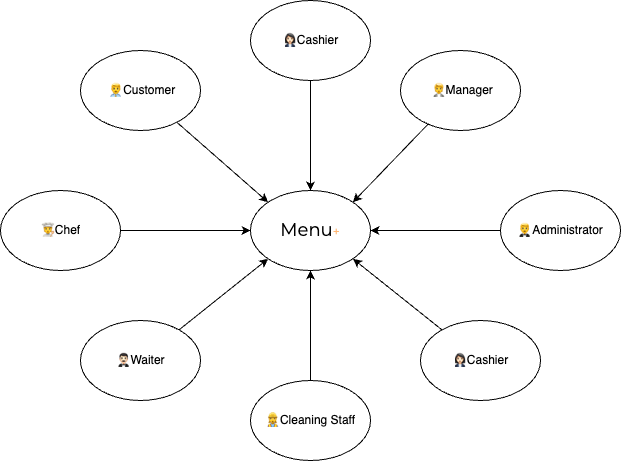
\includegraphics[width=15cm]{Images/OMS-Page-2.png}
	\vspace{0.5cm}
	\caption{Các người dùng trong hệ thống}
	\label{fig:my_label}
\end{figure}

% \begin{table}[h!]
% \centering
% \begin{tabular}{|p{3cm}|p{3cm}|p{9cm}|}
% \hline
% \textbf{Mã đối tượng} & \textbf{Tên} & \textbf{Mô tả} \\ \hline
% US-01 & Customer (Khách hàng) & Xem menu trực tuyến, đặt bàn hoặc order trực tiếp tại nhà hàng, thanh toán và sử dụng mã khuyến mãi. \\ \hline
% US-02 & Cashier (Thu ngân) & Thực hiện xác nhận thanh toán, gộp hoặc tách bill, hỗ trợ khách hàng sử dụng mã khuyến mãi, nhập số tiền nhận và tính tiền thối lại. \\ \hline
% US-03 & Manager (Quản lý) & Quản lý order, doanh thu, nhân sự, chia ca, thêm nhân sự mới, và điều hành chung hệ thống nhà hàng. \\ \hline
% US-04 & Administrator (Quản trị viên) & Quản lý và duy trì hệ thống, cấu hình menu, điều chỉnh các thông tin liên quan đến hệ thống chung. \\ \hline
% US-05 & Chef (Bếp trưởng) & Xem Kitchen Display System (KDS), xác nhận món ăn từ trạng thái "not ready", chuyển sang "cook" và cuối cùng là "ready to serve". \\ \hline
% US-06 & Waiter (Nhân viên phục vụ) & Giúp khách hàng đặt bàn, order món, lấy món ăn từ bếp, phục vụ món ăn, chuyển bàn, thực hiện self-order cho khách, cập nhật trạng thái món ăn là đã phục vụ. \\ \hline
% US-07 & Cleaning Staff (Nhân viên vệ sinh) & Dọn dẹp bàn ăn sau khi khách rời đi, cập nhật tình trạng bàn trên hệ thống để sẵn sàng phục vụ khách tiếp theo. \\ \hline
% \end{tabular}
% \caption{Bảng tổng hợp đối tượng và chức năng trong hệ thống quản lý nhà hàng}
% \label{tab:restaurant_objects}
% \end{table}

\textbf{Các chức năng chính của Menu+}

Hệ thống Menu+ bao gồm các chức năng chính giúp các nhóm người dùng trên thực hiện các công việc hàng ngày một cách hiệu quả và nhanh chóng:

\begin{itemize}


	\item Đặt bàn trực tuyến và quản lý bàn: Giúp khách hàng dễ dàng đặt chỗ và hỗ trợ nhân viên theo dõi trạng thái bàn (trống, đã đặt, đang phục vụ).

	\item Quản lý bàn: Cung cấp công cụ cho nhân viên theo dõi và quản lý bàn trong nhà hàng.

	\item Xử lý đơn hàng: Cho phép nhân viên nhập và gửi đơn hàng đến hệ thống Kitchen Display System (KDS) cho bếp.

	\item Thanh toán và quản lý doanh thu: Tích hợp các phương thức thanh toán đa dạng, tạo thuận tiện cho cả khách hàng và nhà hàng.

	\item Quản lý quan hệ khách hàng (CRM) và nhân sự: Lưu trữ thông tin khách hàng, quản lý lịch làm việc của nhân viên và cung cấp các báo cáo chi tiết về hoạt động kinh doanh.
\end{itemize}

\subsection{Đặc tả chức năng}
\begin{longtable}{|m{1.5cm}|m{3.5cm}|m{4.5cm}|m{5cm}|}
	\caption{Danh sách Người dùng Hệ thống} \label{tab:users}                                                                                                                                                                                                      \\
	\hline
	\textbf{Mã} & \textbf{Tên Người Dùng}    & \textbf{Vai Trò Thực Tế}                                  & \textbf{Mô Tả Ngắn}                                                                                                                                     \\
	\hline
	\endfirsthead

	\hline
	\textbf{Mã} & \textbf{Tên Người Dùng}    & \textbf{Vai Trò Thực Tế}                                  & \textbf{Mô Tả Ngắn}                                                                                                                                     \\
	\hline
	\endhead % Header cho các trang tiếp theo

	\hline
	\endfoot % Footer cho bảng

	\hline
	\endlastfoot % Footer cho trang cuối cùng

	US-01       & Quản lý nhà hàng           & Chủ nhà hàng hoặc người quản lý cấp cao                   & Quản lý tổng thể hoạt động, cấu hình hệ thống (giá bàn, \% đặt cọc, thời gian gọi bot), xem báo cáo toàn diện, quản lý nhân viên và thực đơn.           \\
	\hline
	US-02       & Nhân viên phục vụ          & Waiter/Waitress                                           & Sử dụng POS để nhận đơn hàng tại bàn, quản lý trạng thái bàn, xử lý thanh toán (bao gồm cả việc trừ tiền đặt cọc), tương tác với hệ thống bếp.          \\
	\hline
	US-03       & Nhân viên lễ tân           & Host/Hostess (Có thể là Nhân viên phục vụ đảm nhiệm)      & Quản lý sơ đồ tầng, trạng thái bàn, nhận và quản lý đặt chỗ trực tiếp hoặc qua điện thoại (ít tương tác hệ thống hơn khách hàng tự đặt).                \\
	\hline
	US-04       & Nhân viên bếp              & Chef, Cook, Kitchen Assistant                             & Tương tác chính với Màn hình hiển thị Bếp (KDS) hoặc máy in phiếu bếp để xem chi tiết đơn hàng (bao gồm món đặt trước) và cập nhật trạng thái chuẩn bị. \\
	\hline
	US-05       & Nhân viên thu ngân         & Cashier (Có thể là Nhân viên phục vụ hoặc Quản lý)        & Chịu trách nhiệm đóng/mở phiên POS, đối soát tiền mặt cuối ngày, xử lý các giao dịch thanh toán.                                                        \\
	\hline
	US-06       & Kế toán                    & Accountant/Bookkeeper                                     & Truy cập dữ liệu bán hàng đã được tổng hợp, báo cáo tài chính, quản lý công nợ (nếu có), đối soát doanh thu và tiền đặt cọc.                            \\
	\hline
	US-07       & Nhân viên (Chung)          & Bất kỳ nhân viên nào cần xem lịch làm việc                & Xem lịch làm việc cá nhân được phân công qua Employee Portal, có thể có quyền yêu cầu đổi ca hoặc báo nghỉ.                                             \\
	\hline
	US-08       & Khách hàng                 & Customer/Guest                                            & Tương tác qua giao diện web/app để đặt bàn, đặt món ăn trước, thanh toán đặt cọc, đặt hàng mang về hoặc giao hàng.                                      \\
	\hline
	US-09       & Nhân viên hỗ trợ/ Vận hành & Support/Operations Staff                                  & Tiếp nhận và xử lý các yêu cầu hỗ trợ từ khách hàng.                                                                                                    \\
	\hline
	US-10       & Quản trị viên Hệ thống     & System Administrator (Có thể là Quản lý nhà hàng hoặc IT) & Thực hiện các cấu hình kỹ thuật sâu, quản lý tích hợp (Shipday, Bot), quản lý tài khoản người dùng và phân quyền chi tiết.                              \\
	\hline
\end{longtable}

\newpage % Ngắt trang



\begin{longtable}{|m{2.5cm}|m{2.5cm}|m{5cm}|m{5cm}|}
	\caption{Phân công Chức năng theo Người dùng} \label{tab:user_function_map}                                                                                                                                                            \\
    \hline
	\textbf{Người dùng}                                     & \textbf{Mã chức năng} & \textbf{Tên chức năng}                                 & \textbf{Mô tả ngắn}                                                                         \\
	\hline
	\endfirsthead % Header cho các trang tiếp theo
	
    \hline
	\textbf{Người dùng}                                     & \textbf{Mã chức năng} & \textbf{Tên chức năng}                                 & \textbf{Mô tả ngắn}                                                                         \\
	\hline
	\endhead % Header cho các trang tiếp theo

	\midrule
	\endfoot % Footer cho bảng

	% \bottomrule
	% \endlastfoot % Footer cho trang cuối cùng

	% === US-01: Quản lý nhà hàng ===
	\multicolumn{4}{|l|}{\textbf{US-01: Quản lý nhà hàng}}                                                                                                                                                                                 \\ \hline
	\multirow{15}{=}[2pt]{US-01: Quản lý nhà hàng}          & FR-MD01-01            & Tạo ca làm việc                                        & Cho phép định nghĩa các ca làm việc mới (thời gian, vai trò, số lượng).                     \\
	                                                        & FR-MD01-02            & Gán nhân viên vào ca                                   & Chỉ định nhân viên cụ thể cho các vị trí trống trong ca làm việc.                           \\
	                                                        & FR-MD01-03            & Xem lịch biểu Gantt                                    & Hiển thị lịch làm việc dạng Gantt, lọc theo vai trò, xem theo ngày/tuần/tháng.              \\
	                                                        & FR-MD01-04            & (Kích hoạt) Phát hiện trùng lịch                       & Kích hoạt hệ thống kiểm tra trùng lịch khi gán nhân viên.                                   \\
	                                                        & FR-MD01-05            & Xuất bản và Thông báo lịch                             & Công khai lịch làm việc và kích hoạt gửi thông báo đến nhân viên.                           \\
	                                                        & FR-MD01-07            & Sao chép lịch tuần                                     & Sao chép nhanh lịch làm việc của một tuần sang tuần khác.                                   \\
	                                                        & FR-MD01-08            & Quản lý vai trò công việc                              & Định nghĩa các vai trò công việc trong nhà hàng.                                            \\
	                                                        & FR-MD01-10            & Xem lịch theo vai trò                                  & Lọc và xem lịch làm việc của các nhân viên theo vai trò cụ thể.                             \\ \cline{2-4}
	                                                        & FR-MD02-01            & Tạo Sản phẩm Mới (Món ăn/Đồ uống)                      & Thêm món ăn, đồ uống mới vào hệ thống (tên, giá, loại...).                                  \\
	                                                        & FR-MD02-02            & Chỉnh sửa Thông tin Sản phẩm                           & Cập nhật chi tiết sản phẩm đã có (giá, mô tả, ảnh...).                                      \\
	                                                        & FR-MD02-03            & Lưu trữ/Hủy kích hoạt Sản phẩm                         & Ẩn/Hiện sản phẩm khỏi các giao dịch mà không xóa hẳn.                                       \\
	                                                        & FR-MD02-04            & Quản lý Danh mục Sản phẩm POS                          & Tạo, sửa, xóa, sắp xếp các danh mục hiển thị trên POS.                                      \\
	                                                        & FR-MD02-05            & Định nghĩa Thuộc tính \& Giá trị (cho Biến thể)        & Định nghĩa các đặc tính (size, độ cay) và lựa chọn (S, M, L). (Có thể là US-10)             \\
	                                                        & FR-MD02-06            & Cấu hình Biến thể Sản phẩm                             & Áp dụng thuộc tính/giá trị vào sản phẩm gốc để tạo biến thể, cấu hình giá riêng.            \\
	                                                        & FR-MD02-07            & Thiết lập Loại Sản phẩm                                & Xác định loại sản phẩm (Consumable, Stockable, Service).                                    \\
	                                                        & FR-MD02-08            & Cấu hình Hiển thị trên POS                             & Đánh dấu sản phẩm bán trên POS và gán vào danh mục POS.                                     \\
	                                                        & FR-MD02-09            & Quản lý Hình ảnh Sản phẩm                              & Tải lên, thay thế, xóa hình ảnh đại diện cho sản phẩm.                                      \\
	                                                        & FR-MD02-10            & Cấu hình In Bếp/Hiển thị KDS                           & Chỉ định danh mục sản phẩm nào gửi đến máy in/KDS nào.                                      \\
	                                                        & FR-MD02-11            & Định nghĩa Sản phẩm Tùy chọn/Phụ thu                   & Tạo các sản phẩm nhỏ (Extra cheese) để dùng làm modifier trên POS.                          \\ \cline{2-4}
	                                                        & FR-MD03-11            & Cấu hình Tham số Đặt chỗ                               & Thiết lập giờ hoạt động, giới hạn khách, quy tắc đặt cọc, giá bàn...                        \\
	                                                        & FR-MD03-12            & Xem Danh sách Đặt chỗ                                  & Xem danh sách tổng hợp các lượt đặt chỗ và trạng thái.                                      \\
	                                                        & FR-MD03-13            & Xem Chi tiết Đặt chỗ                                   & Xem thông tin chi tiết của một lượt đặt chỗ cụ thể.                                         \\
	                                                        & FR-MD03-14            & Tạo/Sửa Đặt chỗ Thủ công                               & Tạo hoặc sửa đặt chỗ cho khách qua kênh offline (điện thoại...).                            \\
	                                                        & FR-MD03-15            & Quản lý Trạng thái Đặt chỗ                             & Thay đổi trạng thái đặt chỗ (Xác nhận, Đã đến, Hủy...).                                     \\
	                                                        & FR-MD03-16            & Xem Danh sách Món đặt trước                            & Xem các món cần chuẩn bị cho các đặt chỗ sắp tới.                                           \\ \cline{2-4}
	                                                        & FR-MD04-05            & Cấu hình Dịch vụ Bot Call                              & Cấu hình tham số tích hợp Bot Call (số ngày gọi, kịch bản, số hỗ trợ...). (Có thể là US-10) \\ \cline{2-4}
	                                                        & FR-MD05-01            & Mở phiên làm việc POS                                  & Bắt đầu phiên làm việc POS, nhập tiền mặt đầu ca. (Thường là US-05)                         \\
	                                                        & FR-MD05-13            & Đóng Phiên làm việc POS                                & Kết thúc phiên làm việc, tổng kết, đối chiếu tiền mặt. (Thường là US-05)                    \\
	                                                        & FR-MD05-14            & Chuyển bàn/Ghép bàn                                    & Di chuyển hoặc gộp đơn hàng giữa các bàn.                                                   \\
	                                                        & FR-MD05-15            & Hủy món/Hủy đơn (Void)                                 & Hủy bỏ món hoặc đơn hàng (có thể cần quyền quản lý).                                        \\ \cline{2-4}
	                                                        & FR-MD09-03            & Xem Báo cáo Doanh thu Phiên POS                        & Xem báo cáo tổng kết chi tiết của các phiên POS đã đóng.                                    \\
	                                                        & FR-MD09-04            & Xem Báo cáo Bán hàng theo Sản phẩm/Danh mục            & Xem thống kê số lượng, doanh thu theo từng món ăn/danh mục.                                 \\
	                                                        & FR-MD09-05            & Xem Báo cáo Hiệu suất Nhân viên (POS)                  & Xem doanh thu, số đơn hàng theo từng nhân viên POS.                                         \\
	                                                        & FR-MD09-06            & Xem Báo cáo Tiền đặt cọc                               & Xem báo cáo tổng hợp tình hình thu, sử dụng, mất cọc.                                       \\
	                                                        & FR-MD09-07            & Xem Báo cáo Doanh thu theo Loại hình                   & Phân tích doanh thu theo Eat-in, Takeout, Delivery.                                         \\
	                                                        & FR-MD09-08            & Xuất dữ liệu Báo cáo                                   & Xuất dữ liệu báo cáo ra file Excel/CSV.                                                     \\ \cline{2-4}
	                                                        & FR-MD10-04            & Cấu hình Chung của Hệ thống                            & Cấu hình thông tin công ty, logo, tiền tệ, email... (Có thể là US-10)                       \\
	                                                        & FR-MD10-05            & Cấu hình Tích hợp Bên thứ ba                           & Quản lý API keys cho Cổng thanh toán, Bot Call, Shipday. (Có thể là US-10)                  \\
	                                                        & FR-MD10-06            & Cấu hình Tham số Nghiệp vụ Đặc thù                     & Cấu hình tỷ lệ cọc, giá bàn, số ngày gọi bot... (Có thể là US-10)                           \\
	\hline

	% === US-02: Nhân viên phục vụ ===
	\multicolumn{4}{|l|}{\textbf{US-02: Nhân viên phục vụ}}                                                                                                                                                                                \\ \hline
	\multirow{12}{=}[2pt]{US-02: Nhân viên phục vụ}         & FR-MD05-02            & Truy cập Sơ đồ tầng \& Chọn bàn                        & Xem trạng thái bàn và chọn bàn để phục vụ.                                                  \\
	                                                        & FR-MD05-03            & Bắt đầu/Mở đơn hàng tại bàn                            & Mở giao diện đơn hàng cho bàn đã chọn.                                                      \\
	                                                        & FR-MD05-04            & Tải và Xác nhận Món ăn Đặt trước                       & Xem và xác nhận các món khách đã đặt trước online.                                          \\
	                                                        & FR-MD05-05            & Thêm món ăn/đồ uống vào đơn hàng                       & Nhận order tại bàn và thêm món vào POS.                                                     \\
	                                                        & FR-MD05-06            & Xử lý Yêu cầu đặc biệt/Ghi chú bếp                     & Thêm ghi chú (ít cay, dị ứng...) vào món ăn/đơn hàng.                                       \\
	                                                        & FR-MD05-07            & Gửi đơn hàng xuống Bếp/Bar                             & Gửi thông tin món cần chuẩn bị đến bếp/bar.                                                 \\
	                                                        & FR-MD05-08            & Yêu cầu/In Hóa đơn Tạm tính                            & In bill tạm tính cho khách kiểm tra.                                                        \\
	                                                        & FR-MD05-09            & (Kích hoạt) Áp dụng Tiền Đặt cọc vào Hóa đơn           & Kích hoạt việc trừ cọc khi vào màn hình thanh toán.                                         \\
	                                                        & FR-MD05-10            & Tách hóa đơn (Split Bill)                              & Chia hóa đơn cho khách thanh toán riêng.                                                    \\
	                                                        & FR-MD05-11            & Xử lý Thanh toán                                       & Nhận thanh toán từ khách (tiền mặt, thẻ...), xử lý tiền boa.                                \\
	                                                        & FR-MD05-12            & Đóng Đơn hàng và Bàn                                   & Đóng đơn hàng và giải phóng bàn sau khi khách thanh toán.                                   \\
	                                                        & FR-MD05-14            & Chuyển bàn/Ghép bàn                                    & Di chuyển hoặc gộp đơn hàng giữa các bàn.                                                   \\
	                                                        & FR-MD05-15            & Hủy món/Hủy đơn (Void)                                 & Hủy món/đơn (có thể cần quyền hoặc xác nhận của quản lý).                                   \\ \cline{2-4}
	                                                        & FR-MD06-01            & Chọn Chế độ Bán Mang về                                & Chuyển sang giao diện bán mang về trên POS.                                                 \\
	                                                        & FR-MD06-02            & Tạo Đơn hàng Mang về                                   & Khởi tạo đơn hàng mới cho khách mang về.                                                    \\
	                                                        & FR-MD06-03            & (Tùy chọn) Liên kết Khách hàng                         & Gán đơn hàng mang về với khách hàng (nếu cần).                                              \\
	                                                        & FR-MD06-04            & Thêm món vào Đơn hàng Mang về                          & Thêm món vào đơn hàng mang về.                                                              \\
	                                                        & FR-MD06-05            & Xử lý Ghi chú cho Đơn Mang về                          & Thêm ghi chú cho đơn hàng mang về.                                                          \\
	                                                        & FR-MD06-06            & Gửi đơn Mang về xuống Bếp/Bar                          & Gửi món của đơn mang về xuống bếp/bar.                                                      \\
	                                                        & FR-MD06-07            & (Kích hoạt) Áp dụng Đặt cọc (Nếu Đặt trước Online)     & Kích hoạt trừ cọc cho đơn takeout đặt online.                                               \\
	                                                        & FR-MD06-08            & Thanh toán Đơn hàng Mang về                            & Nhận thanh toán cho đơn hàng mang về tại quầy.                                              \\
	                                                        & FR-MD06-09            & (Nhận) In Hóa đơn/Phiếu thu Mang về                    & Nhận hóa đơn in ra để đưa khách.                                                            \\
	                                                        & FR-MD06-10            & Đóng Đơn hàng Mang về                                  & Đóng đơn hàng mang về sau khi thanh toán/giao hàng.                                         \\ \cline{2-4}
	                                                        & FR-MD07-01            & Chọn Chế độ Giao hàng                                  & Chuyển sang giao diện xử lý đơn giao hàng.                                                  \\
	                                                        & FR-MD07-02            & Tạo/Mở Đơn hàng Giao hàng                              & Tạo/mở đơn hàng giao đi.                                                                    \\
	                                                        & FR-MD07-03            & Liên kết/Nhập Thông tin Khách hàng Giao hàng           & Nhập/chọn thông tin khách và địa chỉ giao hàng.                                             \\
	                                                        & FR-MD07-04            & Thêm món vào Đơn hàng Giao hàng                        & Thêm món vào đơn hàng giao đi.                                                              \\
	                                                        & FR-MD07-05            & Xử lý Ghi chú cho Đơn Giao hàng                        & Thêm ghi chú cho món hoặc cho tài xế.                                                       \\
	                                                        & FR-MD07-06            & Gửi đơn Giao hàng xuống Bếp/Bar                        & Gửi món của đơn giao hàng xuống bếp/bar.                                                    \\
	                                                        & FR-MD07-07            & (Kích hoạt) Áp dụng Đặt cọc/Thanh toán Trước           & Kích hoạt trừ cọc/thanh toán trước cho đơn giao hàng.                                       \\
	                                                        & FR-MD07-08            & Xác nhận và Gửi Đơn hàng sang Shipday                  & Gửi thông tin đơn hàng qua Shipday để điều phối giao hàng.                                  \\
	                                                        & FR-MD07-10            & Xử lý Thanh toán Đơn hàng Giao hàng (Nếu COD)          & Ghi nhận tiền COD tài xế nộp lại.                                                           \\
	                                                        & FR-MD07-11            & In Hóa đơn/Phiếu Giao hàng                             & In phiếu giao hàng/hóa đơn cho tài xế và khách.                                             \\
	                                                        & FR-MD07-12            & Đóng Đơn hàng Giao hàng                                & Đóng đơn hàng giao đi sau khi hoàn tất.                                                     \\
	\hline

	% === US-03: Nhân viên lễ tân ===
	\multicolumn{4}{|l|}{\textbf{US-03: Nhân viên lễ tân}}                                                                                                                                                                                 \\ \hline
	\multirow{5}{=}[2pt]{US-03: Nhân viên lễ tân}           & FR-MD03-12            & Xem Danh sách Đặt chỗ                                  & Xem danh sách tổng hợp các lượt đặt chỗ và trạng thái.                                      \\
	                                                        & FR-MD03-13            & Xem Chi tiết Đặt chỗ                                   & Xem thông tin chi tiết của một lượt đặt chỗ cụ thể.                                         \\
	                                                        & FR-MD03-14            & Tạo/Sửa Đặt chỗ Thủ công                               & Tạo hoặc sửa đặt chỗ cho khách qua kênh offline (điện thoại...).                            \\
	                                                        & FR-MD03-15            & Quản lý Trạng thái Đặt chỗ                             & Thay đổi trạng thái đặt chỗ (Xác nhận, Đã đến, Hủy...).                                     \\ \cline{2-4}
	                                                        & FR-MD05-02            & Truy cập Sơ đồ tầng \& Chọn bàn                        & Xem trạng thái bàn và xếp khách vào bàn (có thể dùng POS).                                  \\
	\hline

	% === US-04: Nhân viên bếp ===
	\multicolumn{4}{|l|}{\textbf{US-04: Nhân viên bếp}}                                                                                                                                                                                    \\ \hline
	\multirow{5}{=}[2pt]{US-04: Nhân viên bếp}              & FR-MD03-16            & Xem Danh sách Món đặt trước                            & Xem các món cần chuẩn bị cho các đặt chỗ sắp tới.                                           \\ \cline{2-4}
	                                                        & FR-MD08-02            & Xem Đơn hàng trên KDS                                  & Xem các đơn hàng/phiếu chờ xử lý trên màn hình KDS.                                         \\
	                                                        & FR-MD08-03            & Thay đổi Trạng thái Món ăn/Đơn hàng trên KDS           & Đánh dấu món/đơn hàng đang làm, đã xong trên KDS.                                           \\
	                                                        & FR-MD08-04            & Xem Chi tiết Món ăn trên KDS                           & Xem chi tiết món ăn, biến thể, ghi chú trên KDS.                                            \\
	                                                        & FR-MD08-05            & (Tùy chọn) Sắp xếp/Ưu tiên Đơn hàng trên KDS           & Sắp xếp hoặc đánh dấu ưu tiên các đơn hàng trên KDS.                                        \\
	                                                        & FR-MD08-07            & Nhận và Xử lý Phiếu in Bếp                             & Nhận phiếu in từ máy in và thực hiện chế biến (thủ công).                                   \\
	\hline

	% === US-05: Nhân viên thu ngân ===
	\multicolumn{4}{|l|}{\textbf{US-05: Nhân viên thu ngân}}                                                                                                                                                                               \\ \hline
	\multirow{11}{=}[2pt]{US-05: Nhân viên thu ngân}        & FR-MD05-01            & Mở phiên làm việc POS                                  & Bắt đầu phiên làm việc POS, nhập tiền mặt đầu ca.                                           \\
	                                                        & FR-MD05-11            & Xử lý Thanh toán                                       & Nhận thanh toán từ khách (tiền mặt, thẻ...), xử lý tiền boa. (Có thể là US-02)              \\
	                                                        & FR-MD05-13            & Đóng Phiên làm việc POS                                & Kết thúc phiên làm việc, tổng kết, đối chiếu tiền mặt.                                      \\ \cline{2-4}
	                                                        & FR-MD06-01            & Chọn Chế độ Bán Mang về                                & Chuyển sang giao diện bán mang về trên POS.                                                 \\
	                                                        & FR-MD06-02            & Tạo Đơn hàng Mang về                                   & Khởi tạo đơn hàng mới cho khách mang về.                                                    \\
	                                                        & FR-MD06-03            & (Tùy chọn) Liên kết Khách hàng                         & Gán đơn hàng mang về với khách hàng (nếu cần).                                              \\
	                                                        & FR-MD06-04            & Thêm món vào Đơn hàng Mang về                          & Thêm món vào đơn hàng mang về.                                                              \\
	                                                        & FR-MD06-05            & Xử lý Ghi chú cho Đơn Mang về                          & Thêm ghi chú cho đơn hàng mang về.                                                          \\
	                                                        & FR-MD06-06            & Gửi đơn Mang về xuống Bếp/Bar                          & Gửi món của đơn mang về xuống bếp/bar.                                                      \\
	                                                        & FR-MD06-08            & Thanh toán Đơn hàng Mang về                            & Nhận thanh toán cho đơn hàng mang về tại quầy.                                              \\
	                                                        & FR-MD06-09            & (Nhận) In Hóa đơn/Phiếu thu Mang về                    & Nhận hóa đơn in ra để đưa khách.                                                            \\
	                                                        & FR-MD06-10            & Đóng Đơn hàng Mang về                                  & Đóng đơn hàng mang về sau khi thanh toán/giao hàng.                                         \\ \cline{2-4}
	                                                        & FR-MD07-01            & Chọn Chế độ Giao hàng                                  & Chuyển sang giao diện xử lý đơn giao hàng.                                                  \\
	                                                        & FR-MD07-02            & Tạo/Mở Đơn hàng Giao hàng                              & Tạo/mở đơn hàng giao đi.                                                                    \\
	                                                        & FR-MD07-03            & Liên kết/Nhập Thông tin Khách hàng Giao hàng           & Nhập/chọn thông tin khách và địa chỉ giao hàng.                                             \\
	                                                        & FR-MD07-04            & Thêm món vào Đơn hàng Giao hàng                        & Thêm món vào đơn hàng giao đi.                                                              \\
	                                                        & FR-MD07-05            & Xử lý Ghi chú cho Đơn Giao hàng                        & Thêm ghi chú cho món hoặc cho tài xế.                                                       \\
	                                                        & FR-MD07-06            & Gửi đơn Giao hàng xuống Bếp/Bar                        & Gửi món của đơn giao hàng xuống bếp/bar.                                                    \\
	                                                        & FR-MD07-08            & Xác nhận và Gửi Đơn hàng sang Shipday                  & Gửi thông tin đơn hàng qua Shipday để điều phối giao hàng.                                  \\
	                                                        & FR-MD07-10            & Xử lý Thanh toán Đơn hàng Giao hàng (Nếu COD)          & Ghi nhận tiền COD tài xế nộp lại.                                                           \\
	                                                        & FR-MD07-11            & In Hóa đơn/Phiếu Giao hàng                             & In phiếu giao hàng/hóa đơn cho tài xế và khách.                                             \\
	                                                        & FR-MD07-12            & Đóng Đơn hàng Giao hàng                                & Đóng đơn hàng giao đi sau khi hoàn tất.                                                     \\
	\hline

	% === US-06: Kế toán ===
	\multicolumn{4}{|l|}{\textbf{US-06: Kế toán}}                                                                                                                                                                                          \\ \hline
	\multirow{5}{=}[2pt]{US-06: Kế toán}                    & FR-MD09-03            & Xem Báo cáo Doanh thu Phiên POS                        & Xem báo cáo tổng kết chi tiết của các phiên POS đã đóng.                                    \\
	                                                        & FR-MD09-04            & Xem Báo cáo Bán hàng theo Sản phẩm/Danh mục            & Xem thống kê số lượng, doanh thu theo từng món ăn/danh mục.                                 \\
	                                                        & FR-MD09-06            & Xem Báo cáo Tiền đặt cọc                               & Xem báo cáo tổng hợp tình hình thu, sử dụng, mất cọc.                                       \\
	                                                        & FR-MD09-07            & Xem Báo cáo Doanh thu theo Loại hình                   & Phân tích doanh thu theo Eat-in, Takeout, Delivery.                                         \\
	                                                        & FR-MD09-08            & Xuất dữ liệu Báo cáo                                   & Xuất dữ liệu báo cáo ra file Excel/CSV.                                                     \\
	\hline

	% === US-07: Nhân viên (Chung) ===
	\multicolumn{4}{|l|}{\textbf{US-07: Nhân viên (Chung)}}                                                                                                                                                                                \\ \hline
	\multirow{2}{=}[2pt]{US-07: Nhân viên (Chung)}          & FR-MD01-06            & Xem lịch cá nhân                                       & Xem lịch làm việc đã được xuất bản của bản thân.                                            \\
	                                                        & FR-MD01-09            & Đánh dấu không sẵn sàng                                & Thông báo cho quản lý về thời gian không thể làm việc.                                      \\
	\hline

	% === US-08: Khách hàng ===
	\multicolumn{4}{|l|}{\textbf{US-08: Khách hàng}}                                                                                                                                                                                       \\ \hline
	\multirow{9}{=}[2pt]{US-08: Khách hàng}                 & FR-MD03-01            & Xem Giao diện Đặt chỗ                                  & Truy cập và xem giao diện đặt chỗ online.                                                   \\
	                                                        & FR-MD03-02            & Chọn Thông tin Đặt bàn                                 & Chọn ngày, giờ, số lượng người đặt bàn.                                                     \\
	                                                        & FR-MD03-03            & (Tùy chọn) Chọn Bàn cụ thể                             & Xem sơ đồ tầng và chọn bàn trống (nếu được phép).                                           \\
	                                                        & FR-MD03-04            & Xem Thực đơn                                           & Xem thực đơn online để chọn món đặt trước.                                                  \\
	                                                        & FR-MD03-05            & Chọn Món ăn Đặt trước                                  & Thêm món ăn/đồ uống vào giỏ hàng đặt trước.                                                 \\
	                                                        & FR-MD03-06            & Xem Tóm tắt Đặt chỗ                                    & Xem lại thông tin đặt bàn, món ăn, tiền cọc dự kiến.                                        \\
	                                                        & FR-MD03-07            & Nhập Thông tin Khách hàng                              & Cung cấp Tên, SĐT, Email.                                                                   \\
	                                                        & FR-MD03-09            & Thanh toán Đặt cọc                                     & Thực hiện thanh toán tiền đặt cọc qua cổng thanh toán.                                      \\
	                                                        & FR-MD03-10            & (Nhận) Xác nhận Đặt chỗ                                & Nhận email/SMS xác nhận sau khi thanh toán thành công.                                      \\
	                                                        & FR-MD03-17            & Xem Lịch sử/Chi tiết Đặt chỗ Cá nhân                   & Xem lại các đặt chỗ đã thực hiện qua tài khoản.                                             \\ \cline{2-4}
	                                                        & FR-MD04-02            & (Tương tác) Thực hiện Cuộc gọi và Tương tác Khách hàng & Nghe máy và bấm phím 1, 0, 2 khi nhận cuộc gọi từ Bot.                                      \\
	\hline

	% === US-09: Nhân viên hỗ trợ/ Vận hành ===
	\multicolumn{4}{|l|}{\textbf{US-09: Nhân viên hỗ trợ/ Vận hành}}                                                                                                                                                                       \\ \hline
	\multirow{1}{=}[2pt]{US-09: Nhân viên hỗ trợ/ Vận hành} & FR-MD04-03            & (Tiếp nhận) Xử lý Phản hồi Khách hàng từ Bot Call      & Nhận cuộc gọi chuyển tiếp từ Bot khi khách bấm phím 2 để hỗ trợ.                            \\
	                                                        &                       &                                                        &
	\tabularnewline\hline
	% === US-10: Quản trị viên Hệ thống ===
	\multicolumn{4}{|l|}{\textbf{US-10: Quản trị viên Hệ thống}}                                                                                                                                                                           \\ \hline
	\multirow{7}{=}[2pt]{US-10: Quản trị viên Hệ thống}     & FR-MD02-05            & Định nghĩa Thuộc tính \& Giá trị (cho Biến thể)        & Định nghĩa các đặc tính (size, độ cay) và lựa chọn (S, M, L). (Có thể là US-01)             \\ \cline{2-4}
	                                                        & FR-MD04-05            & Cấu hình Dịch vụ Bot Call                              & Cấu hình tham số tích hợp Bot Call. (Có thể là US-01)                                       \\ \cline{2-4}
	                                                        & FR-MD07-13            & Cấu hình Tích hợp Shipday                              & Cấu hình tham số kết nối API Shipday. (Có thể là US-01)                                     \\ \cline{2-4}
	                                                        & FR-MD10-01            & Quản lý Người dùng (Nhân viên)                         & Tạo, sửa, vô hiệu hóa tài khoản người dùng nhân viên.                                       \\
	                                                        & FR-MD10-02            & Quản lý Nhóm Quyền                                     & Xem, tạo, sửa, xóa các nhóm quyền truy cập.                                                 \\
	                                                        & FR-MD10-03            & Phân quyền Truy cập cho Người dùng                     & Gán người dùng vào các nhóm quyền phù hợp.                                                  \\
	                                                        & FR-MD10-04            & Cấu hình Chung của Hệ thống                            & Cấu hình thông tin công ty, logo, tiền tệ, email... (Có thể là US-01)                       \\
	                                                        & FR-MD10-05            & Cấu hình Tích hợp Bên thứ ba                           & Quản lý API keys cho Cổng thanh toán, Bot Call, Shipday. (Có thể là US-01)                  \\
	                                                        & FR-MD10-06            & Cấu hình Tham số Nghiệp vụ Đặc thù                     & Cấu hình tỷ lệ cọc, giá bàn, số ngày gọi bot... (Có thể là US-01)                           \\
	                                                        & FR-MD10-07            & Xem Nhật ký Hệ thống (Logs)                            & Xem log hệ thống để theo dõi và khắc phục sự cố.                                            \\
	\hline
\end{longtable}

\newpage


\begin{longtable}{|m{1.5cm}|m{4.5cm}|m{9cm}|}
	\caption{Phân chia Module Hệ thống} \label{tab:modules}                                                                                                                                                                                                                                                                                                                                                                                                                                            \\
	\hline
	\textbf{Mã} & \textbf{Tên Module}                                     & \textbf{Mô Tả}                                                                                                                                                                                                                                                                                                                                                                                                             \\
	\hline
	\endfirsthead % Header cho các trang tiếp theo

	\hline
	\textbf{Mã} & \textbf{Tên Module}                                     & \textbf{Mô Tả}                                                                                                                                                                                                                                                                                                                                                                                                             \\
	\hline
	\endhead % Header cho các trang tiếp theo

	\hline
	\endfoot % Footer cho bảng

	\hline
	\endlastfoot % Footer cho trang cuối cùng

	MD-01       & Quản lý Lịch làm việc (Scheduling)                      & Bao gồm các chức năng: tạo ca làm việc, gán nhân viên theo vai trò, hiển thị dạng Gantt, kiểm tra trùng lịch, xuất bản và thông báo lịch trình cho nhân viên.                                                                                                                                                                                                                                                              \\
	\hline
	MD-02       & Quản lý Thực đơn \& Sản phẩm (Menu \& Product)          & Quản lý danh sách món ăn, đồ uống dưới dạng sản phẩm. Bao gồm tạo mới, chỉnh sửa giá, mô tả, hình ảnh, phân loại theo danh mục POS, quản lý biến thể (ví dụ: size S/M/L), quản lý tồn kho cho các mặt hàng cụ thể (vd: rượu chai).                                                                                                                                                                                         \\
	\hline
	MD-03       & Quản lý Đặt chỗ \& Đặt món trước (Booking \& Pre-order) & Cung cấp giao diện cho khách hàng (web/app) để chọn thời gian, số lượng người, chọn bàn (nếu có), và tùy chọn đặt trước các món ăn từ thực đơn. Tính toán và xử lý thanh toán tiền đặt cọc (15\% giá trị bàn + 15\% giá trị món ăn đặt trước). Quản lý trạng thái các lượt đặt chỗ.                                                                                                                                        \\
	\hline
	MD-04       & Xác nhận Tự động qua Bot (Automated Bot Confirmation)   & Tự động kích hoạt cuộc gọi thoại tới khách hàng trước N ngày (cấu hình được) so với ngày đặt chỗ. Phát thông báo và xử lý lựa chọn của khách (1: Xác nhận, 0: Hủy - cập nhật trạng thái đặt chỗ và ghi nhận mất cọc, 2: Chuyển hướng cuộc gọi đến Nhân viên hỗ trợ).                                                                                                                                                       \\
	\hline
	MD-05       & Quản lý Bán hàng Tại chỗ (POS - Eat-in)                 & Giao diện POS cho nhân viên phục vụ, quản lý sơ đồ tầng, trạng thái bàn, nhận đơn hàng tại bàn (bao gồm cả món khách đã đặt trước), xử lý yêu cầu đặc biệt (ghi chú bếp), tách/gộp hóa đơn, áp dụng tiền đặt cọc đã thanh toán vào hóa đơn cuối cùng, xử lý thanh toán đa phương thức, quản lý tiền boa.                                                                                                                   \\
	\hline
	MD-06       & Quản lý Bán mang về (POS - Takeout)                     & Cung cấp một giao diện/luồng riêng biệt trên POS (ví dụ: nút "Takeout") để tạo đơn hàng mang về. Không yêu cầu chọn bàn. Có thể liên kết với khách hàng nếu họ đã đăng nhập hoặc cung cấp thông tin. Áp dụng tiền đặt cọc nếu đơn hàng được đặt trước qua kênh online. Xử lý thanh toán.                                                                                                                                   \\
	\hline
	MD-07       & Quản lý Giao hàng (POS - Delivery)                      & Cung cấp một giao diện/luồng riêng biệt trên POS (ví dụ: nút "Delivery"). Yêu cầu thông tin khách hàng (đã đăng nhập từ web/app đặt hàng). Tích hợp với Shipday: gửi thông tin đơn hàng (địa chỉ, chi tiết món, thông tin khách) sang Shipday để điều phối tài xế, nhận lại cập nhật trạng thái giao hàng từ Shipday. Áp dụng tiền đặt cọc đã thanh toán. Xử lý thanh toán (có thể là online trước hoặc COD tùy cấu hình). \\
	\hline
	MD-08       & Tích hợp Bếp (Kitchen Integration)                      & Truyền thông tin đơn hàng (từ Eat-in, Takeout, Delivery - bao gồm món đặt trước và ghi chú) tới khu vực bếp thông qua Màn hình hiển thị Bếp (KDS) hoặc máy in phiếu bếp. Cho phép nhân viên bếp cập nhật trạng thái món ăn (đang làm, đã xong).                                                                                                                                                                            \\
	\hline
	MD-09       & Quản lý Phiên \& Báo cáo (Session \& Reporting)         & Quản lý việc mở và đóng phiên làm việc trên POS, đối soát tiền mặt. Cung cấp các báo cáo về doanh thu (theo loại hình: Eat-in, Takeout, Delivery), sản phẩm bán chạy, hiệu suất nhân viên, tiền đặt cọc, trạng thái đơn hàng giao, tích hợp dữ liệu.                                                                                                                                                                       \\
	\hline
	MD-10       & Quản lý Hệ thống \& Người dùng (System \& User)         & Quản lý tài khoản người dùng (tạo, sửa, xóa), phân quyền truy cập chi tiết cho từng vai trò vào các module và chức năng. Quản lý các cấu hình chung như tỷ lệ đặt cọc, giá trị bàn, thời gian gọi bot, cấu hình tích hợp bên thứ ba (API keys,...).                                                                                                                                                                        \\
	\hline
\end{longtable}

\subsubsection{Module MD-01: Quản lý Lịch làm việc (Scheduling)}

Module Quản lý Lịch làm việc (MD-01) là một thành phần cốt lõi của hệ thống quản lý nhà hàng, được thiết kế để hỗ trợ Quản lý nhà hàng trong việc lập kế hoạch, phân công và theo dõi lịch trình làm việc của nhân viên một cách hiệu quả và tối ưu. Module này bao gồm một loạt các chức năng từ việc định nghĩa các vai trò công việc cơ bản, tạo khung ca làm việc, gán nhân viên cụ thể vào ca, cho đến việc xuất bản lịch và cho phép nhân viên xem lịch trình cá nhân của mình.

\begin{figure}[H]
    \centering
    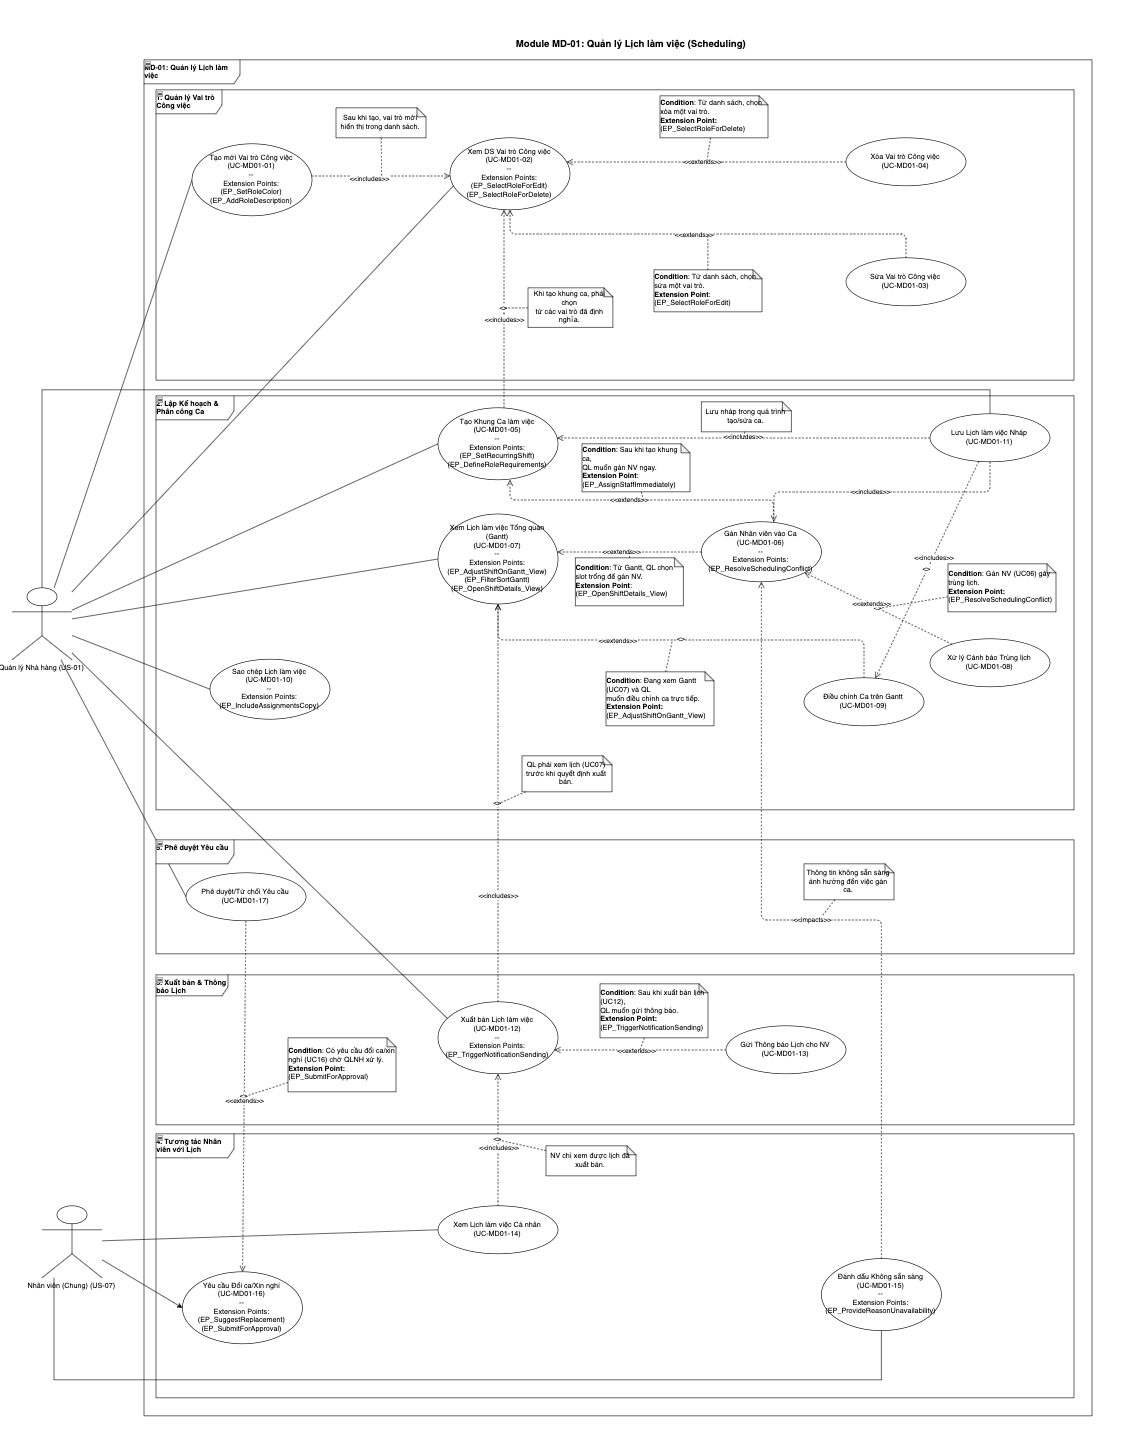
\includegraphics[width=15cm]{Sections/tong_quan/functional_spec/img/uc1.png}
    \vspace{0.5cm}
    \caption{Use case diagram cho Module MD-01}
    \label{fig:my_label}
\end{figure}

\begin{longtable}{|m{2cm}|m{2.5cm}|m{2cm}|m{4cm}|m{4.5cm}|}
    \caption{Danh sách Yêu cầu Chức năng cho Module MD-01: Quản lý Lịch làm việc} \label{tab:fr_md01_revised} \\
    \hline
    \textbf{Mã Module} & \textbf{Mã Yêu cầu CN} & \textbf{Mã Người dùng} & \textbf{Tên Chức năng} & \textbf{Mô tả Ngắn} \\
    \hline
    \endhead
    
    \hline
    \endfoot
    
    \hline
    \endlastfoot
    
    MD-01 & FR-MD01-01 & US-01 & Tạo mới Vai trò Công việc & Cho phép Quản lý nhà hàng định nghĩa một vai trò công việc mới (ví dụ: Bếp trưởng, Phục vụ). \\
    \hline
    MD-01 & FR-MD01-02 & US-01 & Xem Danh sách Vai trò Công việc & Cho phép Quản lý nhà hàng xem danh sách các vai trò công việc đã được định nghĩa. \\
    \hline
    MD-01 & FR-MD01-03 & US-01 & Sửa Thông tin Vai trò Công việc & Cho phép Quản lý nhà hàng chỉnh sửa thông tin của một vai trò công việc hiện có. \\
    \hline
    MD-01 & FR-MD01-04 & US-01 & Xóa Vai trò Công việc & Cho phép Quản lý nhà hàng xóa một vai trò công việc không còn sử dụng (nếu thỏa điều kiện). \\
    \hline
    MD-01 & FR-MD01-05 & US-01 & Tạo Khung Ca làm việc & Cho phép Quản lý nhà hàng định nghĩa các khung ca làm việc (thời gian, ngày, yêu cầu vai trò, số lượng). \\
    \hline
    MD-01 & FR-MD01-06 & US-01 & Gán Nhân viên vào Ca làm việc & Cho phép Quản lý nhà hàng chỉ định nhân viên cụ thể cho các vị trí trong khung ca đã tạo. \\
    \hline
    MD-01 & FR-MD01-07 & US-01 & Xem Lịch làm việc Tổng quan (Gantt) & Hiển thị lịch làm việc của tất cả nhân viên hoặc lọc theo vai trò dưới dạng biểu đồ Gantt. \\
    \hline
    MD-01 & FR-MD01-08 & US-01 & Xử lý Cảnh báo Trùng lịch & Khi hệ thống phát hiện trùng lịch (tự động), cho phép Quản lý nhà hàng xem xét và điều chỉnh việc gán ca để giải quyết xung đột. \\
    \hline
    MD-01 & FR-MD01-09 & US-01 & Điều chỉnh Ca làm việc trên Gantt & Cho phép Quản lý nhà hàng kéo thả, thay đổi kích thước, hoặc sửa đổi trực tiếp các ca trên biểu đồ Gantt. \\
    \hline
    MD-01 & FR-MD01-10 & US-01 & Sao chép Lịch làm việc (Ngày/Tuần/Tùy chỉnh) & Cho phép Quản lý nhà hàng sao chép nhanh lịch của một ngày, một tuần, hoặc một khoảng thời gian tùy chọn sang một thời điểm khác. \\
    \hline
    MD-01 & FR-MD01-11 & US-01 & Lưu Lịch làm việc Nháp & Cho phép Quản lý nhà hàng lưu lại các thay đổi trong lịch trình dưới dạng bản nháp. \\
    \hline
    MD-01 & FR-MD01-12 & US-01 & Xuất bản Lịch làm việc & Cho phép Quản lý nhà hàng công khai (publish) lịch làm việc đã được hoàn thiện. \\
    \hline
    MD-01 & FR-MD01-13 & US-01 & Gửi Thông báo Lịch làm việc cho Nhân viên & Kích hoạt hệ thống gửi thông báo (email/app) đến từng nhân viên về lịch trình cá nhân của họ sau khi lịch được xuất bản. \\
    \hline
    MD-01 & FR-MD01-14 & US-07 & Xem Lịch làm việc Cá nhân & Cho phép Nhân viên xem lịch làm việc đã được xuất bản của riêng mình. \\
    \hline
    MD-01 & FR-MD01-15 & US-07 & Đánh dấu Khoảng thời gian Không sẵn sàng & Cho phép Nhân viên (nếu được cấu hình) thông báo các khoảng thời gian không thể làm việc. \\
    \hline
    MD-01 & FR-MD01-16 & US-07 & Yêu cầu Đổi ca/Xin nghỉ & Cho phép Nhân viên (nếu được cấu hình) gửi yêu cầu đổi ca hoặc xin nghỉ thông qua hệ thống. \\
    \hline
    MD-01 & FR-MD01-17 & US-01 & Phê duyệt/Từ chối Yêu cầu Đổi ca/Xin nghỉ & Cho phép Quản lý nhà hàng xem xét và quyết định các yêu cầu đổi ca/xin nghỉ từ nhân viên. \\
    \hline
    
    \end{longtable}

\subsubsubsection{Mục tiêu và Phạm vi}
\label{sssec:md01_objectives_scope}
Mục tiêu chính của module MD-01 là:
\begin{itemize}
    \item \textbf{Tối ưu hóa việc sử dụng nhân lực:} Đảm bảo đủ nhân sự cho từng ca làm việc dựa trên nhu cầu hoạt động của nhà hàng, tránh tình trạng thiếu hoặc thừa nhân viên.
    \item \textbf{Minh bạch hóa lịch trình:} Cung cấp một cái nhìn tổng quan và chi tiết về lịch làm việc cho cả quản lý và nhân viên, giúp mọi người nắm rõ kế hoạch.
    \item \textbf{Giảm thiểu xung đột lịch trình:} Phát hiện và hỗ trợ giải quyết các trường hợp trùng lịch của nhân viên.
    \item \textbf{Tăng cường hiệu quả quản lý:} Tiết kiệm thời gian và công sức cho Quản lý nhà hàng trong việc lập lịch thủ công.
    \item \textbf{Cải thiện giao tiếp:} Tự động hóa việc thông báo lịch trình mới hoặc thay đổi cho nhân viên.
\end{itemize}
Phạm vi của module bao gồm toàn bộ quy trình quản lý lịch làm việc, từ khâu thiết lập ban đầu (vai trò công việc) đến khi lịch được công bố và nhân viên có thể tương tác (xem lịch, yêu cầu thay đổi).

\subsubsubsection{Đối tượng Sử dụng Chính}
\label{sssec:md01_primary_users}
Module này chủ yếu phục vụ hai nhóm đối tượng người dùng:
\begin{itemize}
    \item \textbf{US-01 (Quản lý nhà hàng):} Là người dùng chính, chịu trách nhiệm thực hiện hầu hết các chức năng của module như tạo vai trò, tạo khung ca, gán nhân viên, điều chỉnh lịch, xuất bản lịch, và phê duyệt các yêu cầu từ nhân viên.
    \item \textbf{US-07 (Nhân viên):} Là người dùng cuối, có thể xem lịch làm việc cá nhân đã được xuất bản, đánh dấu khoảng thời gian không sẵn sàng, và (tùy chọn) gửi yêu cầu đổi ca hoặc xin nghỉ.
\end{itemize}

\subsubsubsection{Các Chức năng Chính}
\label{sssec:md01_key_functionalities}
Module MD-01 cung cấp một bộ các chức năng toàn diện, được mô tả chi tiết qua các Use Case sau:

\begin{itemize}
    \item \textbf{Quản lý Vai trò Công việc (UC-MD01-01 đến UC-MD01-04):}
    \begin{itemize}
        \item Cho phép định nghĩa các vai trò công việc mới (ví dụ: "Đầu bếp chính", "Phục vụ bàn").
        \item Xem danh sách, sửa thông tin, và xóa các vai trò không còn sử dụng (với điều kiện ràng buộc).
    \end{itemize}

    \item \textbf{Lập Kế hoạch và Phân công Ca làm việc (UC-MD01-05, UC-MD01-06, UC-MD01-10, UC-MD01-11):}
    \begin{itemize}
        \item Tạo các khung ca làm việc, xác định thời gian và nhu cầu nhân sự (số lượng, vai trò) cho từng ca.
        \item Gán nhân viên cụ thể vào các vị trí còn trống trong khung ca, dựa trên sự phù hợp về vai trò và tính khả dụng.
        \item Sao chép lịch làm việc từ một ngày/tuần đã có sang ngày/tuần mới để tiết kiệm thời gian.
        \item Lưu trữ các thay đổi dưới dạng lịch nháp trước khi công bố.
    \end{itemize}

    \item \textbf{Trực quan hóa và Điều chỉnh Lịch (UC-MD01-07, UC-MD01-08, UC-MD01-09):}
    \begin{itemize}
        \item Hiển thị lịch làm việc tổng quan dưới dạng biểu đồ Gantt, cho phép lọc và nhóm theo nhân viên hoặc vai trò, thay đổi khung thời gian xem.
        \item Tự động phát hiện và cảnh báo các trường hợp trùng lịch của nhân viên, hỗ trợ Quản lý xử lý.
        \item Cho phép điều chỉnh nhanh ca làm việc (thay đổi thời gian, di chuyển ca, gán lại nhân viên) trực tiếp trên biểu đồ Gantt.
    \end{itemize}

    \item \textbf{Xuất bản và Thông báo Lịch (UC-MD01-12, UC-MD01-13):}
    \begin{itemize}
        \item Chính thức hóa lịch làm việc đã được xếp (chuyển từ "Nháp" sang "Đã xuất bản").
        \item Tự động gửi thông báo lịch làm việc cá nhân đến từng nhân viên sau khi lịch được xuất bản.
    \end{itemize}

    \item \textbf{Tương tác của Nhân viên (UC-MD01-14, UC-MD01-15, UC-MD01-16):}
    \begin{itemize}
        \item Cho phép nhân viên xem lịch làm việc cá nhân đã được xuất bản.
        \item Cho phép nhân viên chủ động đánh dấu các khoảng thời gian họ không thể làm việc.
        \item (Tùy chọn) Cho phép nhân viên gửi yêu cầu đổi ca hoặc xin nghỉ cho các ca đã được phân công.
    \end{itemize}

    \item \textbf{Quản lý Yêu cầu Nhân viên (UC-MD01-17):}
    \begin{itemize}
        \item (Tùy chọn) Cho phép Quản lý nhà hàng xem xét và phê duyệt hoặc từ chối các yêu cầu đổi ca/xin nghỉ từ nhân viên.
    \end{itemize}
\end{itemize}

\subsubsubsection{Tóm tắt Luồng Hoạt động Tổng thể}
\label{sssec:md01_overall_workflow}
Luồng hoạt động chính trong module MD-01 thường diễn ra như sau:
\begin{enumerate}
    \item \textbf{Thiết lập ban đầu:} Quản lý nhà hàng định nghĩa các Vai trò Công việc cần thiết (UC-MD01-01).
    \item \textbf{Tạo khung ca:} Quản lý tạo các Khung Ca làm việc cho một khoảng thời gian (ví dụ: tuần), xác định nhu cầu về số lượng và vai trò cho mỗi ca (UC-MD01-05). Có thể sử dụng chức năng Sao chép lịch để tăng tốc (UC-MD01-10).
    \item \textbf{Phân công nhân viên:} Quản lý gán từng Nhân viên cụ thể vào các vị trí trong khung ca (UC-MD01-06). Hệ thống hỗ trợ bằng cách gợi ý nhân viên phù hợp và cảnh báo nếu có thông tin không sẵn sàng (UC-MD01-15).
    \item \textbf{Rà soát và điều chỉnh:} Quản lý xem Lịch làm việc Tổng quan trên Gantt (UC-MD01-07), phát hiện và Xử lý Cảnh báo Trùng lịch (UC-MD01-08), và thực hiện các Điều chỉnh Ca cần thiết (UC-MD01-09). Mọi thay đổi được Lưu Nháp (UC-MD01-11).
    \item \textbf{Xuất bản và thông báo:} Sau khi hoàn tất, Quản lý Xuất bản Lịch làm việc (UC-MD01-12), và hệ thống Gửi Thông báo cho Nhân viên (UC-MD01-13).
    \item \textbf{Nhân viên tương tác:} Nhân viên Xem Lịch làm việc Cá nhân (UC-MD01-14). Nếu được phép, họ có thể Yêu cầu Đổi ca/Xin nghỉ (UC-MD01-16).
    \item \textbf{Xử lý yêu cầu:} Quản lý Phê duyệt/Từ chối các yêu cầu từ nhân viên (UC-MD01-17), và cập nhật lại lịch nếu cần.
\end{enumerate}
Module MD-01 đóng vai trò trung tâm trong việc đảm bảo hoạt động trơn tru hàng ngày của nhà hàng bằng cách quản lý hiệu quả nguồn lực quan trọng nhất: con người.

\subsubsection{Module MD-02: Quản lý Thực đơn \& Sản phẩm}
Module Quản lý Thực đơn \& Sản phẩm (MD-02) là một thành phần trung tâm trong hệ thống quản lý nhà hàng, đóng vai trò quan trọng trong việc định nghĩa, tổ chức và quản lý tất cả các mặt hàng mà nhà hàng cung cấp, từ món ăn, đồ uống đến các dịch vụ đi kèm. Module này cho phép Quản lý nhà hàng duy trì một cơ sở dữ liệu sản phẩm chính xác và chi tiết, làm nền tảng cho các hoạt động bán hàng, quản lý tồn kho (nếu có), và hiển thị trên giao diện Point of Sale (POS).


\begin{figure}[H]
    \centering
    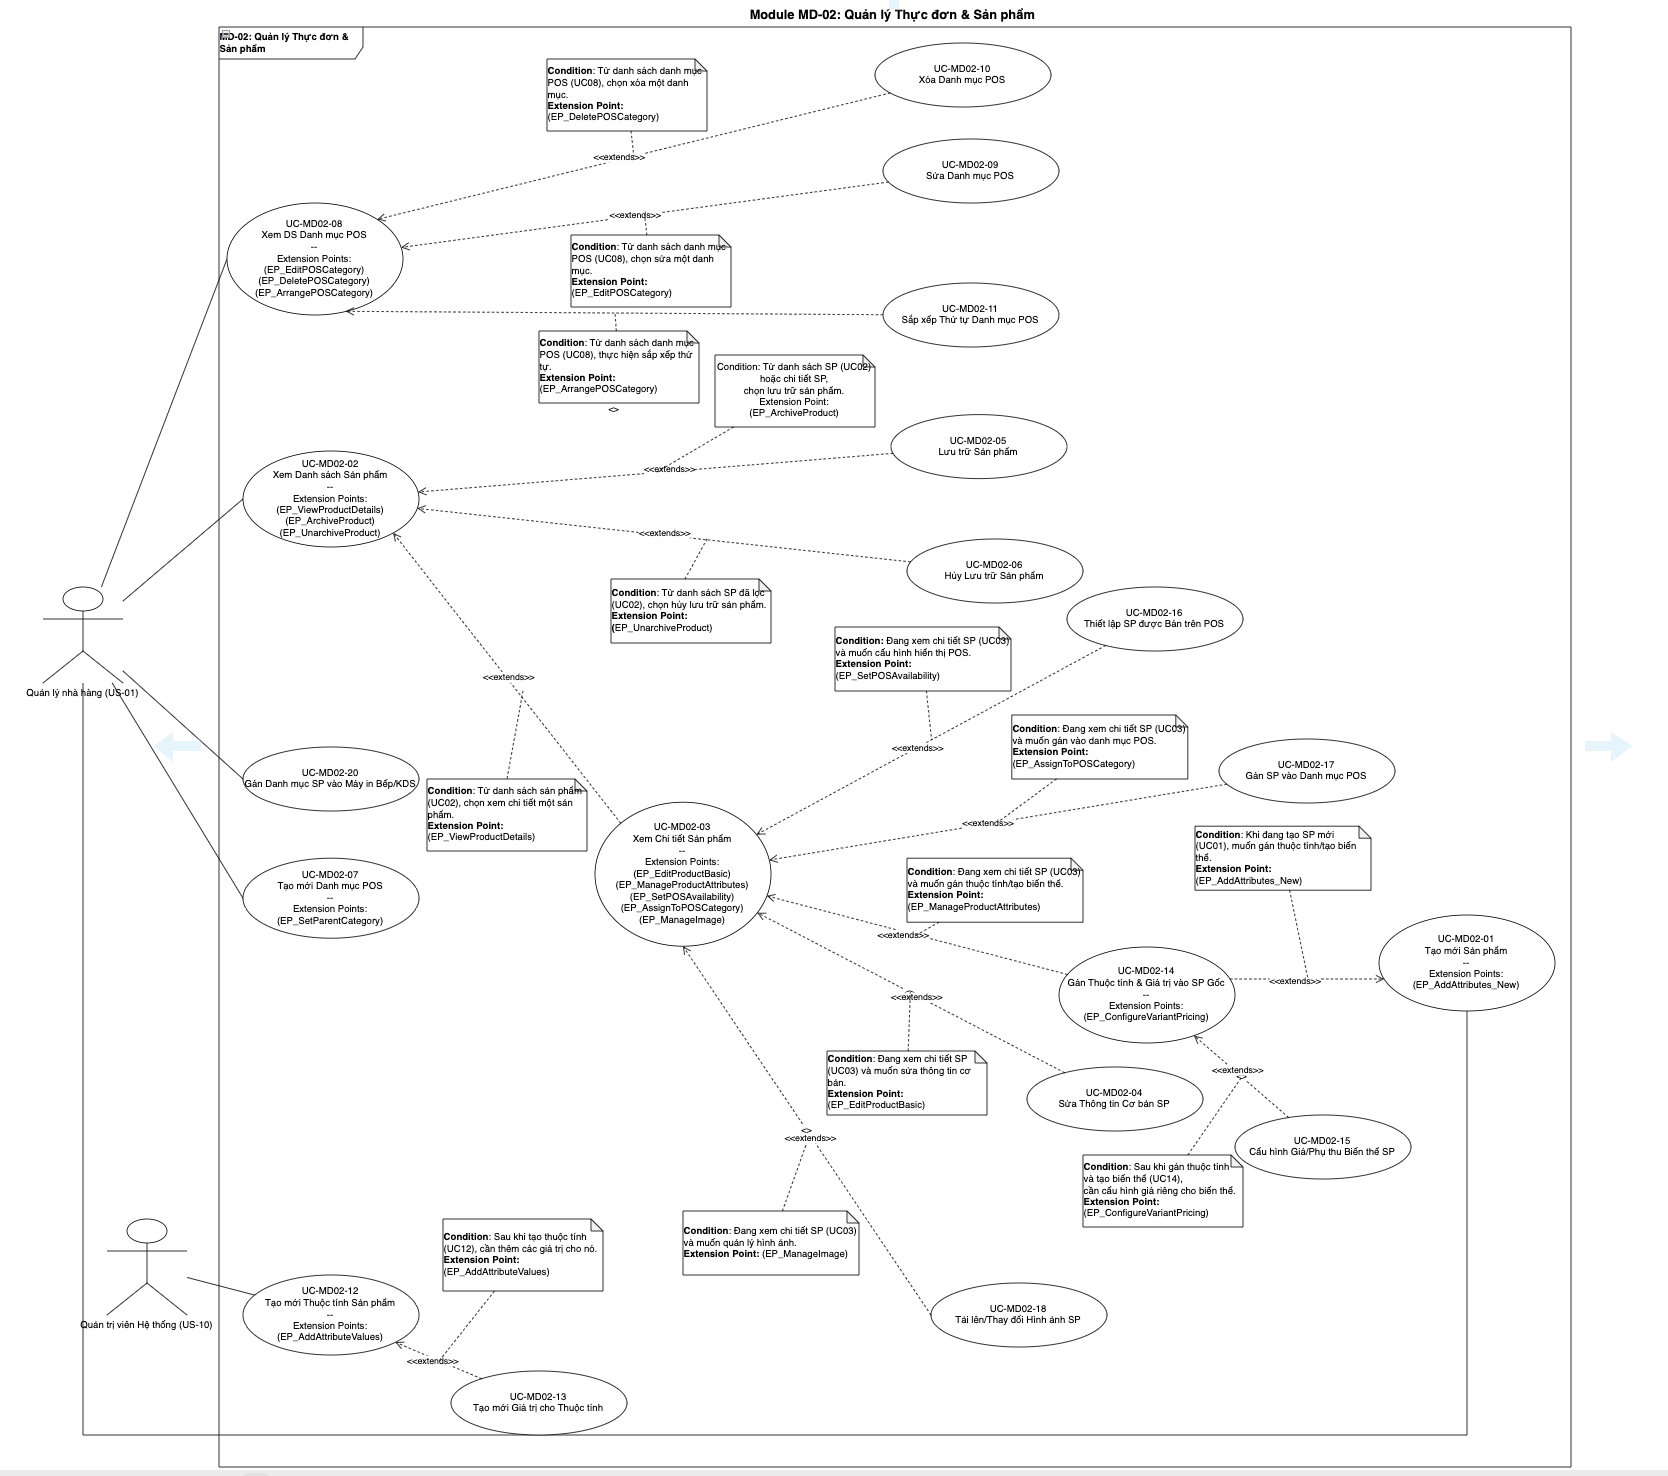
\includegraphics[width=15cm]{Sections/tong_quan/functional_spec/img/uc2.png}
    \vspace{0.5cm}
    \caption{Use case diagram cho Module MD-02}
    \label{fig:my_label}
\end{figure}

\begin{longtable}{|m{2cm}|m{2.5cm}|m{2cm}|m{4.5cm}|m{4cm}|}
\caption{Danh sách Yêu cầu Chức năng cho Module MD-02: Quản lý Thực đơn \& Sản phẩm} \label{tab:fr_md02_revised} \\
\hline
\textbf{Mã Module} & \textbf{Mã Yêu cầu CN} & \textbf{Mã Người dùng} & \textbf{Tên Chức năng} & \textbf{Mô tả Ngắn} \\
\hline
\endhead % Header cho các trang tiếp theo

\hline
\endfoot % Footer cho bảng

\hline
\endlastfoot % Footer cho trang cuối cùng

MD-02 & FR-MD02-01 & US-01 & Tạo mới Sản phẩm & Cho phép Quản lý nhà hàng thêm một món ăn, đồ uống, hoặc dịch vụ mới vào hệ thống (Tên, Giá, Loại...). \\
\hline
MD-02 & FR-MD02-02 & US-01 & Xem Danh sách Sản phẩm & Cho phép Quản lý nhà hàng xem danh sách tất cả các sản phẩm hiện có trong hệ thống. \\
\hline
MD-02 & FR-MD02-03 & US-01 & Xem Chi tiết Sản phẩm & Cho phép Quản lý nhà hàng xem thông tin chi tiết đầy đủ của một sản phẩm cụ thể. \\
\hline
MD-02 & FR-MD02-04 & US-01 & Sửa Thông tin Cơ bản của Sản phẩm & Cho phép Quản lý nhà hàng cập nhật các thông tin chung của sản phẩm (Tên, Loại, Giá bán, Giá vốn, Mã nội bộ...). \\
\hline
MD-02 & FR-MD02-05 & US-01 & Lưu trữ Sản phẩm & Cho phép Quản lý nhà hàng ẩn một sản phẩm khỏi các giao dịch mà không xóa hẳn dữ liệu (Archive). \\
\hline
MD-02 & FR-MD02-06 & US-01 & Hủy Lưu trữ Sản phẩm & Cho phép Quản lý nhà hàng kích hoạt lại một sản phẩm đã bị lưu trữ để bán/sử dụng lại (Unarchive). \\
\hline
MD-02 & FR-MD02-07 & US-01 & Tạo mới Danh mục POS & Cho phép Quản lý nhà hàng tạo một danh mục mới để nhóm sản phẩm trên giao diện POS. \\
\hline
MD-02 & FR-MD02-08 & US-01 & Xem Danh sách Danh mục POS & Cho phép Quản lý nhà hàng xem danh sách các danh mục POS đã tạo. \\
\hline
MD-02 & FR-MD02-09 & US-01 & Sửa Danh mục POS & Cho phép Quản lý nhà hàng chỉnh sửa thông tin (Tên, Thứ tự, Cha...) của một danh mục POS. \\
\hline
MD-02 & FR-MD02-10 & US-01 & Xóa Danh mục POS & Cho phép Quản lý nhà hàng xóa một danh mục POS (nếu thỏa điều kiện). \\
\hline
MD-02 & FR-MD02-11 & US-01 & Sắp xếp Thứ tự Danh mục POS & Cho phép Quản lý nhà hàng thay đổi thứ tự hiển thị của các danh mục POS. \\
\hline
MD-02 & FR-MD02-12 & US-01/US-10 & Tạo mới Thuộc tính Sản phẩm & Cho phép định nghĩa một đặc tính mới cho sản phẩm (ví dụ: Kích cỡ, Màu sắc). \\
\hline
MD-02 & FR-MD02-13 & US-01/US-10 & Tạo mới Giá trị cho Thuộc tính & Cho phép định nghĩa các lựa chọn cụ thể cho một thuộc tính (ví dụ: S, M, L cho Kích cỡ). \\
\hline
MD-02 & FR-MD02-14 & US-01 & Gán Thuộc tính và Giá trị vào Sản phẩm Gốc & Cho phép Quản lý nhà hàng áp dụng các thuộc tính và giá trị đã định nghĩa vào một sản phẩm gốc. \\
\hline
MD-02 & FR-MD02-15 & US-01 & Cấu hình Giá/Phụ thu cho Biến thể Sản phẩm & Cho phép Quản lý nhà hàng đặt giá bán khác nhau hoặc giá trị phụ thu cho từng biến thể sản phẩm cụ thể. \\
\hline
MD-02 & FR-MD02-16 & US-01 & Thiết lập Sản phẩm được Bán trên POS & Cho phép Quản lý nhà hàng đánh dấu một sản phẩm là có sẵn để bán trên POS. \\
\hline
MD-02 & FR-MD02-17 & US-01 & Gán Sản phẩm vào Danh mục POS & Cho phép Quản lý nhà hàng chỉ định một sản phẩm thuộc về (các) danh mục nào trên POS. \\
\hline
MD-02 & FR-MD02-18 & US-01 & Tải lên/Thay đổi Hình ảnh Sản phẩm & Cho phép Quản lý nhà hàng quản lý hình ảnh đại diện cho sản phẩm. \\
\hline
MD-02 & FR-MD02-19 & US-01 & Xóa Hình ảnh Sản phẩm & Cho phép Quản lý nhà hàng xóa hình ảnh hiện tại của sản phẩm. \\
\hline
MD-02 & FR-MD02-20 & US-01 & Gán Danh mục Sản phẩm vào Máy in Bếp/KDS & Cho phép Quản lý nhà hàng chỉ định danh mục sản phẩm nào sẽ gửi đến thiết bị bếp/KDS nào (Cấu hình này thường nằm trong Cài đặt POS). \\
\hline

\end{longtable}

\subsubsubsection{Mục tiêu và Phạm vi}
\label{sssec:md02_objectives_scope}
Mục tiêu chính của module MD-02 là:
\begin{itemize}
    \item \textbf{Quản lý tập trung danh mục sản phẩm:} Cung cấp một nơi duy nhất để tạo, sửa, xóa và xem thông tin chi tiết của tất cả các món ăn, đồ uống, và dịch vụ.
    \item \textbf{Hỗ trợ định giá linh hoạt:} Cho phép thiết lập giá bán, giá vốn, và quản lý giá cho các biến thể sản phẩm khác nhau.
    \item \textbf{Tổ chức thực đơn cho POS:} Cho phép tạo và quản lý các danh mục sản phẩm để hiển thị một cách khoa học và dễ sử dụng trên màn hình Point of Sale.
    \item \textbf{Quản lý biến thể sản phẩm:} Hỗ trợ tạo và quản lý các phiên bản khác nhau của cùng một sản phẩm (ví dụ: kích cỡ, độ cay, topping) với các mức giá tương ứng.
    \item \textbf{Tích hợp với các module khác:} Đảm bảo dữ liệu sản phẩm được sử dụng nhất quán trong các module Bán hàng, Kho (Inventory), Kế toán, và Point of Sale.
    \item \textbf{Cấu hình hiển thị và in ấn:} Cho phép tùy chỉnh hình ảnh sản phẩm và cấu hình cách các đơn hàng được gửi đến máy in bếp hoặc Màn hình Hiển thị Bếp (KDS).
\end{itemize}
Phạm vi của module bao gồm toàn bộ vòng đời của một sản phẩm trong hệ thống, từ việc tạo mới, cấu hình chi tiết, quản lý các thuộc tính và biến thể, tổ chức hiển thị trên POS, cho đến việc lưu trữ hoặc ngừng kinh doanh sản phẩm.

\subsubsubsection{Đối tượng Sử dụng Chính}
\label{sssec:md02_primary_users}
Module này chủ yếu được sử dụng bởi:
\begin{itemize}
    \item \textbf{US-01 (Quản lý nhà hàng):} Là người dùng chính, chịu trách nhiệm thực hiện hầu hết các chức năng của module như tạo mới sản phẩm, cập nhật giá, quản lý danh mục POS, cấu hình biến thể, và thiết lập hiển thị trên POS.
    \item \textbf{US-10 (Quản trị viên Hệ thống):} Có thể tham gia vào việc tạo và quản lý các Thuộc tính sản phẩm dùng chung hoặc các cấu hình hệ thống liên quan đến sản phẩm.
\end{itemize}
Nhân viên bán hàng (US-03) sẽ tương tác gián tiếp với module này thông qua giao diện POS, nơi họ chọn các sản phẩm đã được cấu hình.

\subsubsubsection{Các Chức năng Chính}
\label{sssec:md02_key_functionalities}
Module MD-02 cung cấp một loạt các chức năng thiết yếu, được mô tả chi tiết qua các Use Case sau:

\begin{itemize}
    \item \textbf{Quản lý Thông tin Sản phẩm Cơ bản (UC-MD02-01 đến UC-MD02-06, UC-MD02-18, UC-MD02-19):}
    \begin{itemize}
        \item Tạo mới một sản phẩm (món ăn, đồ uống, dịch vụ) với các thông tin ban đầu như tên, loại, giá bán, giá vốn (UC-MD02-01).
        \item Xem danh sách toàn bộ sản phẩm với các tùy chọn tìm kiếm, lọc và nhóm (UC-MD02-02).
        \item Xem thông tin chi tiết đầy đủ của một sản phẩm cụ thể (UC-MD02-03).
        \item Sửa đổi các thông tin cơ bản của sản phẩm đã tồn tại (UC-MD02-04).
        \item Lưu trữ (ẩn đi) các sản phẩm không còn kinh doanh và hủy lưu trữ khi cần (UC-MD02-05, UC-MD02-06).
        \item Tải lên, thay đổi hoặc xóa hình ảnh đại diện cho sản phẩm (UC-MD02-18, UC-MD02-19).
    \end{itemize}

    \item \textbf{Quản lý Danh mục Point of Sale (POS) (UC-MD02-07 đến UC-MD02-11):}
    \begin{itemize}
        \item Tạo mới các danh mục để phân loại sản phẩm trên giao diện POS (ví dụ: "Khai vị", "Món chính") (UC-MD02-07).
        \item Xem, sửa, xóa và sắp xếp thứ tự hiển thị của các danh mục POS (UC-MD02-08, UC-MD02-09, UC-MD02-10, UC-MD02-11).
    \end{itemize}

    \item \textbf{Quản lý Thuộc tính và Biến thể Sản phẩm (UC-MD02-12 đến UC-MD02-15):}
    \begin{itemize}
        \item Tạo mới các thuộc tính chung cho sản phẩm (ví dụ: "Kích cỡ", "Màu sắc", "Độ cay") (UC-MD02-12).
        \item Định nghĩa các giá trị cụ thể cho từng thuộc tính (ví dụ: "Nhỏ", "Vừa", "Lớn" cho thuộc tính "Kích cỡ") (UC-MD02-13).
        \item Gán các thuộc tính và giá trị đã chọn vào một sản phẩm gốc, từ đó tự động tạo ra các sản phẩm biến thể (UC-MD02-14).
        \item Cấu hình giá bán riêng hoặc mức phụ thu cho từng biến thể sản phẩm cụ thể (UC-MD02-15).
    \end{itemize}

    \item \textbf{Cấu hình Sản phẩm cho Point of Sale (UC-MD02-16, UC-MD02-17, UC-MD02-20):}
    \begin{itemize}
        \item Thiết lập cho phép hoặc không cho phép một sản phẩm được bán trên giao diện POS (UC-MD02-16).
        \item Gán một sản phẩm vào một hoặc nhiều danh mục POS để hiển thị đúng nhóm trên menu (UC-MD02-17).
        \item Cấu hình việc định tuyến các danh mục sản phẩm đến các máy in bếp hoặc màn hình KDS cụ thể khi có đơn hàng (UC-MD02-20).
    \end{itemize}
\end{itemize}

\subsubsubsection{Tóm tắt Luồng Hoạt động Tổng thể}
\label{sssec:md02_overall_workflow}
Luồng hoạt động điển hình trong module Quản lý Thực đơn \& Sản phẩm bao gồm các bước chính sau:
\begin{enumerate}
    \item \textbf{Tạo sản phẩm mới:} Quản lý nhà hàng Tạo mới Sản phẩm với các thông tin cơ bản như tên, giá, loại (UC-MD02-01).
    \item \textbf{Cấu hình chi tiết sản phẩm:}
        \begin{itemize}
            \item Tải lên Hình ảnh Sản phẩm (UC-MD02-18).
            \item Nếu sản phẩm có nhiều phiên bản, Quản lý sẽ Tạo mới Thuộc tính (UC-MD02-12), Tạo mới Giá trị cho Thuộc tính (UC-MD02-13), Gán Thuộc tính và Giá trị vào Sản phẩm Gốc để tạo biến thể (UC-MD02-14), và Cấu hình Giá/Phụ thu cho Biến thể (UC-MD02-15).
        \end{itemize}
    \item \textbf{Chuẩn bị cho POS:}
        \begin{itemize}
            \item Quản lý Tạo mới Danh mục POS nếu cần (UC-MD02-07) hoặc Sắp xếp Thứ tự Danh mục POS (UC-MD02-11).
            \item Thiết lập Sản phẩm được Bán trên POS (UC-MD02-16).
            \item Gán Sản phẩm vào Danh mục POS tương ứng (UC-MD02-17).
            \item Gán Danh mục Sản phẩm vào Máy in Bếp/KDS để định tuyến đơn hàng (UC-MD02-20).
        \end{itemize}
    \item \textbf{Bảo trì và cập nhật:}
        \begin{itemize}
            \item Quản lý thường xuyên Xem Danh sách Sản phẩm (UC-MD02-02) và Xem Chi tiết Sản phẩm (UC-MD02-03).
            \item Thực hiện Sửa Thông tin Cơ bản của Sản phẩm khi cần (ví dụ: thay đổi giá) (UC-MD02-04).
            \item Lưu trữ Sản phẩm không còn kinh doanh (UC-MD02-05) hoặc Hủy Lưu trữ Sản phẩm khi muốn bán lại (UC-MD02-06).
            \item Quản lý Danh mục POS: Sửa (UC-MD02-09) hoặc Xóa (UC-MD02-10) khi cần thiết.
        \end{itemize}
\end{enumerate}
Module MD-02 đảm bảo rằng thực đơn của nhà hàng luôn được cập nhật, chính xác và được trình bày một cách tối ưu trên các hệ thống bán hàng, góp phần vào trải nghiệm khách hàng tốt và hiệu quả vận hành.

\subsubsection{Module MD-03: Quản lý Đặt chỗ \& Đặt món trước}
Module Quản lý Đặt chỗ \& Đặt món trước (MD-03) được thiết kế để cung cấp một giải pháp toàn diện cho nhà hàng trong việc quản lý các yêu cầu đặt bàn từ khách hàng, cả qua kênh trực tuyến lẫn các kênh truyền thống. Module này không chỉ giúp tối ưu hóa việc sử dụng không gian và nguồn lực của nhà hàng mà còn nâng cao trải nghiệm của khách hàng bằng cách cho phép họ chủ động tìm kiếm, lựa chọn thời gian, bàn (tùy chọn), và thậm chí đặt trước các món ăn mong muốn.



\begin{figure}[H]
    \centering
    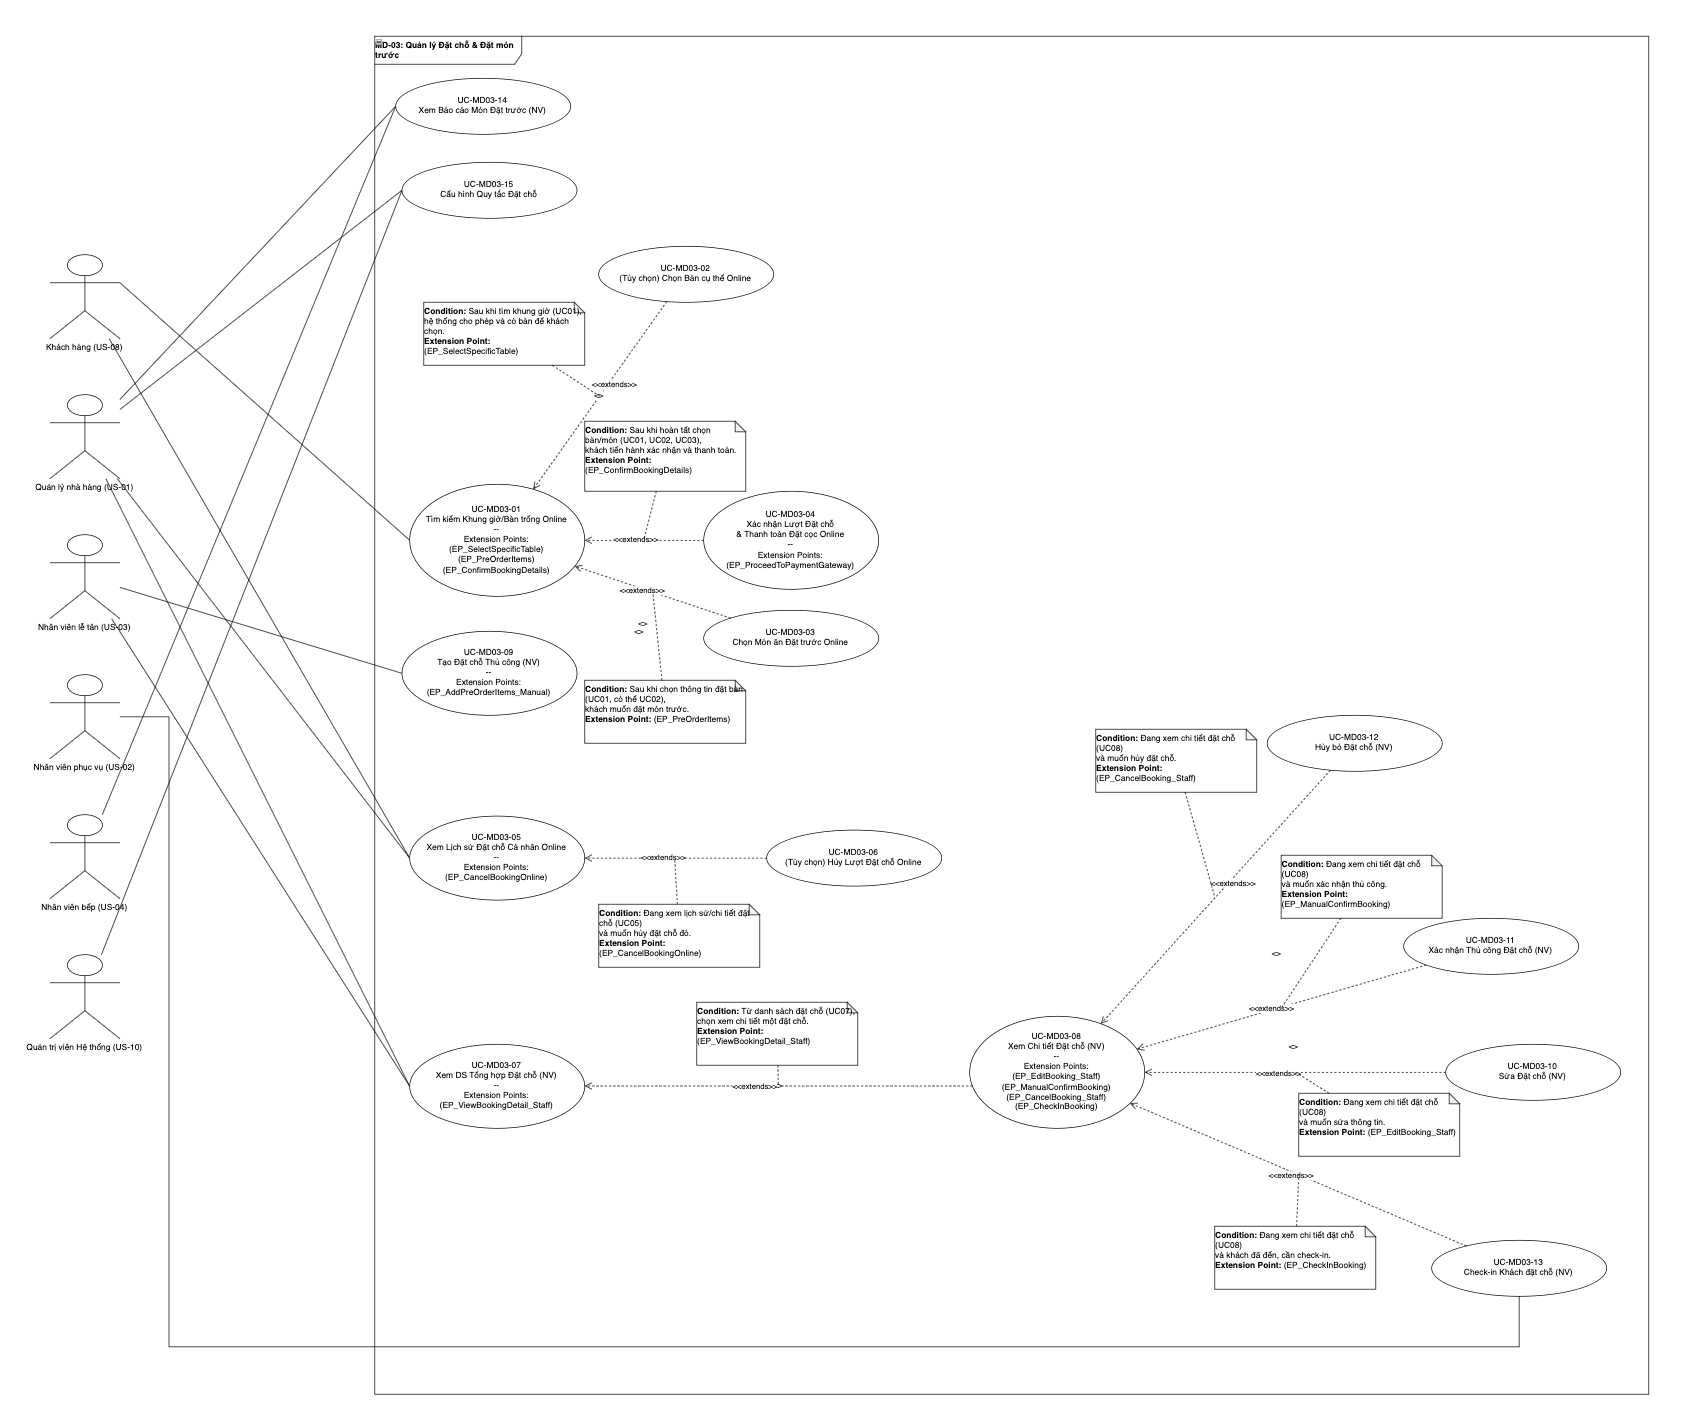
\includegraphics[width=15cm]{Sections/tong_quan/functional_spec/img/uc3.png}
    \vspace{0.5cm}
    \caption{Use case diagram cho Module MD-03}
    \label{fig:my_label}
\end{figure}

\begin{longtable}{|m{2cm}|m{2.5cm}|m{2cm}|m{4.5cm}|m{4cm}|}
\caption{Danh sách Yêu cầu Chức năng cho Module MD-03: Quản lý Đặt chỗ \& Đặt món trước} \label{tab:fr_md03_revised_v3} \\
\hline
\textbf{Mã Module} & \textbf{Mã Yêu cầu CN} & \textbf{Mã Người dùng} & \textbf{Tên Chức năng} & \textbf{Mô tả Ngắn} \\
\hline
\endhead % Header cho các trang tiếp theo
\hline
\endfoot % Footer cho bảng
\hline
\endlastfoot % Footer cho trang cuối cùng

% === Luồng Khách hàng Đặt Online ===
MD-03 & FR-MD03-01 & US-08 & Tìm kiếm Khung giờ/Bàn trống Online & Khách hàng nhập ngày, giờ, số người để tìm kiếm các lựa chọn đặt bàn còn trống. \\
\hline
MD-03 & FR-MD03-02 & US-08 & (Tùy chọn) Chọn Bàn cụ thể từ Sơ đồ tầng Online & Khách hàng xem sơ đồ và chọn bàn trống cụ thể (nếu được phép). \\
\hline
MD-03 & FR-MD03-03 & US-08 & Chọn Món ăn Đặt trước từ Thực đơn Online & Khách hàng duyệt thực đơn và thêm các món muốn đặt trước vào giỏ hàng. \\
\hline
MD-03 & FR-MD03-04 & US-08 & Xác nhận Lượt Đặt chỗ và Thanh toán Đặt cọc Online & Khách hàng xem lại toàn bộ thông tin, nhập thông tin cá nhân và thực hiện thanh toán tiền đặt cọc. \\
\hline
MD-03 & FR-MD03-05 & US-08 & Xem Lịch sử Đặt chỗ Cá nhân Online & Khách hàng đã đăng nhập xem lại các đặt chỗ đã thực hiện. \\
\hline
MD-03 & FR-MD03-06 & US-08 & (Tùy chọn) Hủy Lượt Đặt chỗ Online & Khách hàng hủy một đặt chỗ đã xác nhận (nếu còn trong thời hạn và chính sách cho phép). \\
\hline

% === Luồng Nhân viên Quản lý Đặt chỗ ===
MD-03 & FR-MD03-07 & US-01/US-03 & Xem Danh sách Tổng hợp các Lượt Đặt chỗ & Nhân viên xem danh sách tất cả các đặt chỗ với bộ lọc/tìm kiếm. \\
\hline
MD-03 & FR-MD03-08 & US-01/US-03 & Xem Thông tin Chi tiết một Lượt Đặt chỗ & Nhân viên xem đầy đủ chi tiết của một đặt chỗ cụ thể. \\
\hline
MD-03 & FR-MD03-09 & US-01/US-03 & Tạo mới Lượt Đặt chỗ Thủ công (Backend/POS) & Nhân viên nhập thông tin để tạo đặt chỗ cho khách qua điện thoại/trực tiếp. \\
\hline
MD-03 & FR-MD03-10 & US-01/US-03 & Sửa Thông tin Lượt Đặt chỗ (Backend/POS) & Nhân viên cập nhật các thông tin của một đặt chỗ đã có. \\
\hline
MD-03 & FR-MD03-11 & US-01/US-03 & Xác nhận Thủ công Lượt Đặt chỗ & Nhân viên chuyển trạng thái một đặt chỗ (ví dụ: từ chờ sang đã xác nhận). \\
\hline
MD-03 & FR-MD03-12 & US-01/US-03 & Hủy bỏ Lượt Đặt chỗ (Backend/POS) & Nhân viên hủy một đặt chỗ, có thể kèm lý do. \\
\hline
MD-03 & FR-MD03-13 & US-01/US-03 & Đánh dấu Khách đã đến (Check-in) cho Lượt Đặt chỗ & Nhân viên ghi nhận khách đã đến nhận bàn. \\
\hline
MD-03 & FR-MD03-14 & US-04/US-01 & Xem Báo cáo Tổng hợp Món ăn Cần chuẩn bị (Đặt trước) & Nhân viên bếp/quản lý xem các món đã được khách đặt trước. \\
\hline

% === Luồng Cấu hình ===
MD-03 & FR-MD03-15 & US-01/US-10 & Cấu hình Quy tắc và Tham số Đặt chỗ & Thiết lập giờ, giới hạn khách, quy tắc cọc, giá trị bàn, cho phép chọn bàn online... \\
\hline

\end{longtable}



\subsubsubsection{Mục tiêu và Phạm vi}
\label{sssec:md03_objectives_scope}
Mục tiêu chính của module MD-03 bao gồm:
\begin{itemize}
    \item \textbf{Tối ưu hóa quy trình đặt chỗ:} Tự động hóa việc tìm kiếm và xác nhận đặt bàn, giảm thiểu công việc thủ công cho nhân viên.
    \item \textbf{Nâng cao trải nghiệm khách hàng:} Cung cấp giao diện trực tuyến thân thiện cho khách hàng tự tìm kiếm, đặt bàn, chọn món và thanh toán đặt cọc.
    \item \textbf{Quản lý hiệu quả tình trạng bàn:} Cung cấp cái nhìn tổng quan về tình trạng đặt bàn, giúp nhân viên sắp xếp và quản lý khách hiệu quả hơn.
    \item \textbf{Giảm thiểu tình trạng no-show:} Thông qua việc yêu cầu đặt cọc (nếu có) và gửi thông báo nhắc nhở.
    \item \textbf{Hỗ trợ chuẩn bị cho bếp:} Nếu có chức năng đặt món trước, cung cấp thông tin sớm cho bộ phận bếp để chuẩn bị nguyên liệu và chế biến.
    \item \textbf{Linh hoạt trong cấu hình:} Cho phép nhà hàng tùy chỉnh các quy tắc đặt chỗ (giờ hoạt động, giới hạn khách, chính sách đặt cọc) cho phù hợp với mô hình kinh doanh.
\end{itemize}
Phạm vi của module bao gồm toàn bộ quy trình từ khi khách hàng bắt đầu tìm kiếm đặt chỗ online, chọn món (nếu có), thanh toán đặt cọc, nhận xác nhận, cho đến khi nhân viên nhà hàng quản lý các lượt đặt chỗ này, cập nhật trạng thái (check-in, hủy), và xem báo cáo liên quan.

\subsubsubsection{Đối tượng Sử dụng Chính}
\label{sssec:md03_primary_users}
Module này phục vụ các nhóm đối tượng người dùng sau:
\begin{itemize}
    \item \textbf{US-08 (Khách hàng):} Là người dùng chính của các chức năng đặt chỗ trực tuyến, bao gồm tìm kiếm bàn trống, chọn món, thanh toán đặt cọc và xem lại lịch sử đặt chỗ.
    \item \textbf{US-01 (Quản lý nhà hàng):} Chịu trách nhiệm cấu hình các quy tắc đặt chỗ, xem báo cáo, quản lý các lượt đặt chỗ có vấn đề, và có thể thực hiện tất cả các thao tác quản lý đặt chỗ.
    \item \textbf{US-03 (Nhân viên lễ tân):} Thường xuyên làm việc với module để xem danh sách đặt chỗ, tạo đặt chỗ thủ công, sửa thông tin, xác nhận, hủy, và đánh dấu khách đã đến.
    \item \textbf{US-04 (Nhân viên bếp):} (Nếu có đặt món trước) Xem báo cáo các món ăn cần chuẩn bị.
    \item \textbf{US-10 (Quản trị viên Hệ thống):} Có thể tham gia vào việc cấu hình các tham số hệ thống sâu hơn liên quan đến module đặt chỗ.
\end{itemize}

\subsubsubsection{Các Chức năng Chính}
\label{sssec:md03_key_functionalities}
Module MD-03 cung cấp một tập hợp các chức năng đa dạng, được mô tả chi tiết qua các Use Case sau:

\begin{itemize}
    \item \textbf{Đặt chỗ Trực tuyến từ Khách hàng (UC-MD03-01 đến UC-MD03-06):}
    \begin{itemize}
        \item Cho phép khách hàng tìm kiếm khung giờ và bàn trống dựa trên ngày, giờ và số lượng người (UC-MD03-01).
        \item (Tùy chọn) Cho phép khách hàng chọn một bàn cụ thể từ sơ đồ tầng online (UC-MD03-02).
        \item Cho phép khách hàng duyệt thực đơn và chọn các món ăn/đồ uống để đặt trước (UC-MD03-03).
        \item Khách hàng xem lại thông tin, cung cấp chi tiết liên hệ và thực hiện thanh toán đặt cọc (nếu có) để xác nhận đặt chỗ (UC-MD03-04).
        \item Cho phép khách hàng đã đăng nhập xem lại lịch sử các lượt đặt chỗ cá nhân (UC-MD03-05).
        \item (Tùy chọn) Cho phép khách hàng tự hủy một lượt đặt chỗ đã xác nhận, tuân theo chính sách của nhà hàng (UC-MD03-06).
    \end{itemize}

    \item \textbf{Quản lý Lượt Đặt chỗ bởi Nhân viên (UC-MD03-07 đến UC-MD03-13):}
    \begin{itemize}
        \item Cho phép nhân viên xem danh sách tổng hợp các lượt đặt chỗ với khả năng lọc và tìm kiếm (UC-MD03-07).
        \item Tạo mới một lượt đặt chỗ thủ công trong hệ thống (ví dụ: cho khách đặt qua điện thoại) (UC-MD03-09).
        \item Xem thông tin chi tiết đầy đủ của một lượt đặt chỗ cụ thể (UC-MD03-08).
        \item Sửa đổi các thông tin của một lượt đặt chỗ đã tồn tại (UC-MD03-10).
        \item Xác nhận thủ công một lượt đặt chỗ (ví dụ: chuyển từ "Chờ xác nhận" sang "Đã xác nhận") (UC-MD03-11).
        \item Hủy bỏ một lượt đặt chỗ trong hệ thống (UC-MD03-12).
        \item Đánh dấu khách hàng đã đến (check-in) cho một lượt đặt chỗ (UC-MD03-13).
    \end{itemize}

    \item \textbf{Báo cáo và Cấu hình (UC-MD03-14, UC-MD03-15):}
    \begin{itemize}
        \item Cung cấp báo cáo tổng hợp các món ăn cần chuẩn bị cho các lượt đặt chỗ có đặt món trước (UC-MD03-14).
        \item Cho phép Quản lý/Quản trị viên cấu hình các quy tắc và tham số vận hành cho chức năng đặt chỗ (UC-MD03-15).
    \end{itemize}
\end{itemize}

\subsubsubsection{Tóm tắt Luồng Hoạt động Tổng thể}
\label{sssec:md03_overall_workflow}
Luồng hoạt động chính trong module MD-03 có thể được tóm tắt như sau:

\begin{enumerate}
    \item \textbf{Cấu hình ban đầu:} Quản lý nhà hàng Cấu hình Quy tắc và Tham số Đặt chỗ (UC-MD03-15) như giờ hoạt động, chính sách đặt cọc, v.v.
    \item \textbf{Khách hàng đặt chỗ online:}
        \begin{itemize}
            \item Khách hàng Tìm kiếm Khung giờ/Bàn trống Online (UC-MD03-01).
            \item (Tùy chọn) Khách hàng Chọn Bàn cụ thể từ Sơ đồ tầng Online (UC-MD03-02).
            \item (Tùy chọn) Khách hàng Chọn Món ăn Đặt trước từ Thực đơn Online (UC-MD03-03).
            \item Khách hàng Xác nhận Lượt Đặt chỗ và Thanh toán Đặt cọc Online (UC-MD03-04).
        \end{itemize}
    \item \textbf{Nhân viên quản lý đặt chỗ:}
        \begin{itemize}
            \item Nhân viên thường xuyên Xem Danh sách Tổng hợp các Lượt Đặt chỗ (UC-MD03-07) và Xem Thông tin Chi tiết một Lượt Đặt chỗ (UC-MD03-08).
            \item Nhân viên có thể Tạo mới Lượt Đặt chỗ Thủ công (UC-MD03-09) cho khách đặt qua kênh khác.
            \item Thực hiện Sửa Thông tin Lượt Đặt chỗ (UC-MD03-10) nếu khách yêu cầu thay đổi.
            \item Xác nhận Thủ công Lượt Đặt chỗ (UC-MD03-11) nếu cần.
            \item Hủy bỏ Lượt Đặt chỗ (UC-MD03-12) nếu khách yêu cầu hoặc nhà hàng cần hủy.
            \item Khi khách đến, nhân viên Đánh dấu Khách đã đến (Check-in) (UC-MD03-13).
        \end{itemize}
    \item \textbf{Tương tác sau đặt chỗ của khách hàng (nếu đăng nhập):}
        \begin{itemize}
            \item Khách hàng có thể Xem Lịch sử Đặt chỗ Cá nhân Online (UC-MD03-05).
            \item (Tùy chọn) Khách hàng có thể Hủy Lượt Đặt chỗ Online (UC-MD03-06) nếu chính sách cho phép.
        \end{itemize}
    \item \textbf{Chuẩn bị và báo cáo:}
        \begin{itemize}
            \item Bộ phận bếp/Quản lý Xem Báo cáo Tổng hợp Món ăn Cần chuẩn bị từ các đơn đặt món trước (UC-MD03-14).
        \end{itemize}
\end{enumerate}
Module MD-03 là một công cụ mạnh mẽ giúp nhà hàng không chỉ quản lý hiệu quả các lượt đặt chỗ mà còn tương tác tốt hơn với khách hàng, từ đó cải thiện chất lượng dịch vụ và tối ưu hóa hoạt động kinh doanh.

\subsubsection{Module MD-04: Xác nhận Tự động qua Bot}

\begin{longtable}{|m{2cm}|m{2.5cm}|m{2.5cm}|m{4.5cm}|m{3.5cm}|}
\caption{Danh sách Yêu cầu Chức năng cho Module MD-04: Xác nhận Tự động qua Bot} \label{tab:fr_md04} \\
\hline
\textbf{Mã Module} & \textbf{Mã Yêu cầu CN} & \textbf{Mã Người dùng} & \textbf{Tên Chức năng} & \textbf{Mô tả Ngắn} \\
\hline
\endhead % Header cho các trang tiếp theo

\hline
\endfoot % Footer cho bảng

\hline
\endlastfoot % Footer cho trang cuối cùng

MD-04 & FR-MD04-01 & System & Lên lịch và Kích hoạt Cuộc gọi Xác nhận & Tự động xác định các đặt chỗ 'Đã xác nhận' sắp diễn ra và lên lịch kích hoạt cuộc gọi xác nhận N ngày trước ngày đặt (N cấu hình được). \\
\hline
MD-04 & FR-MD04-02 & System (Bot Service), US-08 (Tương tác) & Thực hiện Cuộc gọi và Tương tác Khách hàng & Tích hợp với dịch vụ Bot Call bên ngoài để thực hiện cuộc gọi đến SĐT khách hàng, phát thông điệp và nhận lựa chọn (phím 1, 0, 2). \\
\hline
MD-04 & FR-MD04-03 & System, US-09 (Tiếp nhận cuộc gọi hỗ trợ) & Xử lý Phản hồi Khách hàng từ Bot Call & Cập nhật trạng thái đặt chỗ và thực hiện hành động tương ứng (xác nhận lại, hủy bỏ & giải phóng bàn, chuyển cuộc gọi hỗ trợ) dựa trên phím khách hàng đã bấm. \\
\hline
MD-04 & FR-MD04-04 & System & Ghi nhận Kết quả Cuộc gọi & Lưu trữ lại kết quả của mỗi cuộc gọi Bot Call (thành công, thất bại, không liên lạc được, lựa chọn của khách) vào thông tin đặt chỗ hoặc nhật ký hệ thống. \\
\hline
MD-04 & FR-MD04-05 & US-01 / US-10 & Cấu hình Dịch vụ Bot Call & Cho phép cấu hình các tham số tích hợp Bot Call: số ngày N gọi trước, nội dung kịch bản thoại, số điện thoại chuyển tiếp hỗ trợ, API key/credentials của dịch vụ Bot Call. \\
\hline

\end{longtable}


\subsubsection{Module MD-05: Quản lý Bán hàng Tại chỗ (POS - Eat-in)}
Module Quản lý Bán hàng Tại chỗ (MD-05), thường được biết đến với tên gọi Point of Sale (POS) cho dịch vụ ăn tại nhà hàng (Eat-in), là giao diện và hệ thống nghiệp vụ cốt lõi mà nhân viên phục vụ và thu ngân sử dụng để quản lý toàn bộ quy trình phục vụ khách hàng tại bàn. Từ việc mở ca làm việc, chọn bàn, nhận đơn hàng, gửi yêu cầu xuống bếp, xử lý các thay đổi, cho đến việc thanh toán và đóng đơn, module này đóng vai trò trung tâm trong hoạt động hàng ngày của nhà hàng.



\begin{figure}[H]
    \centering
    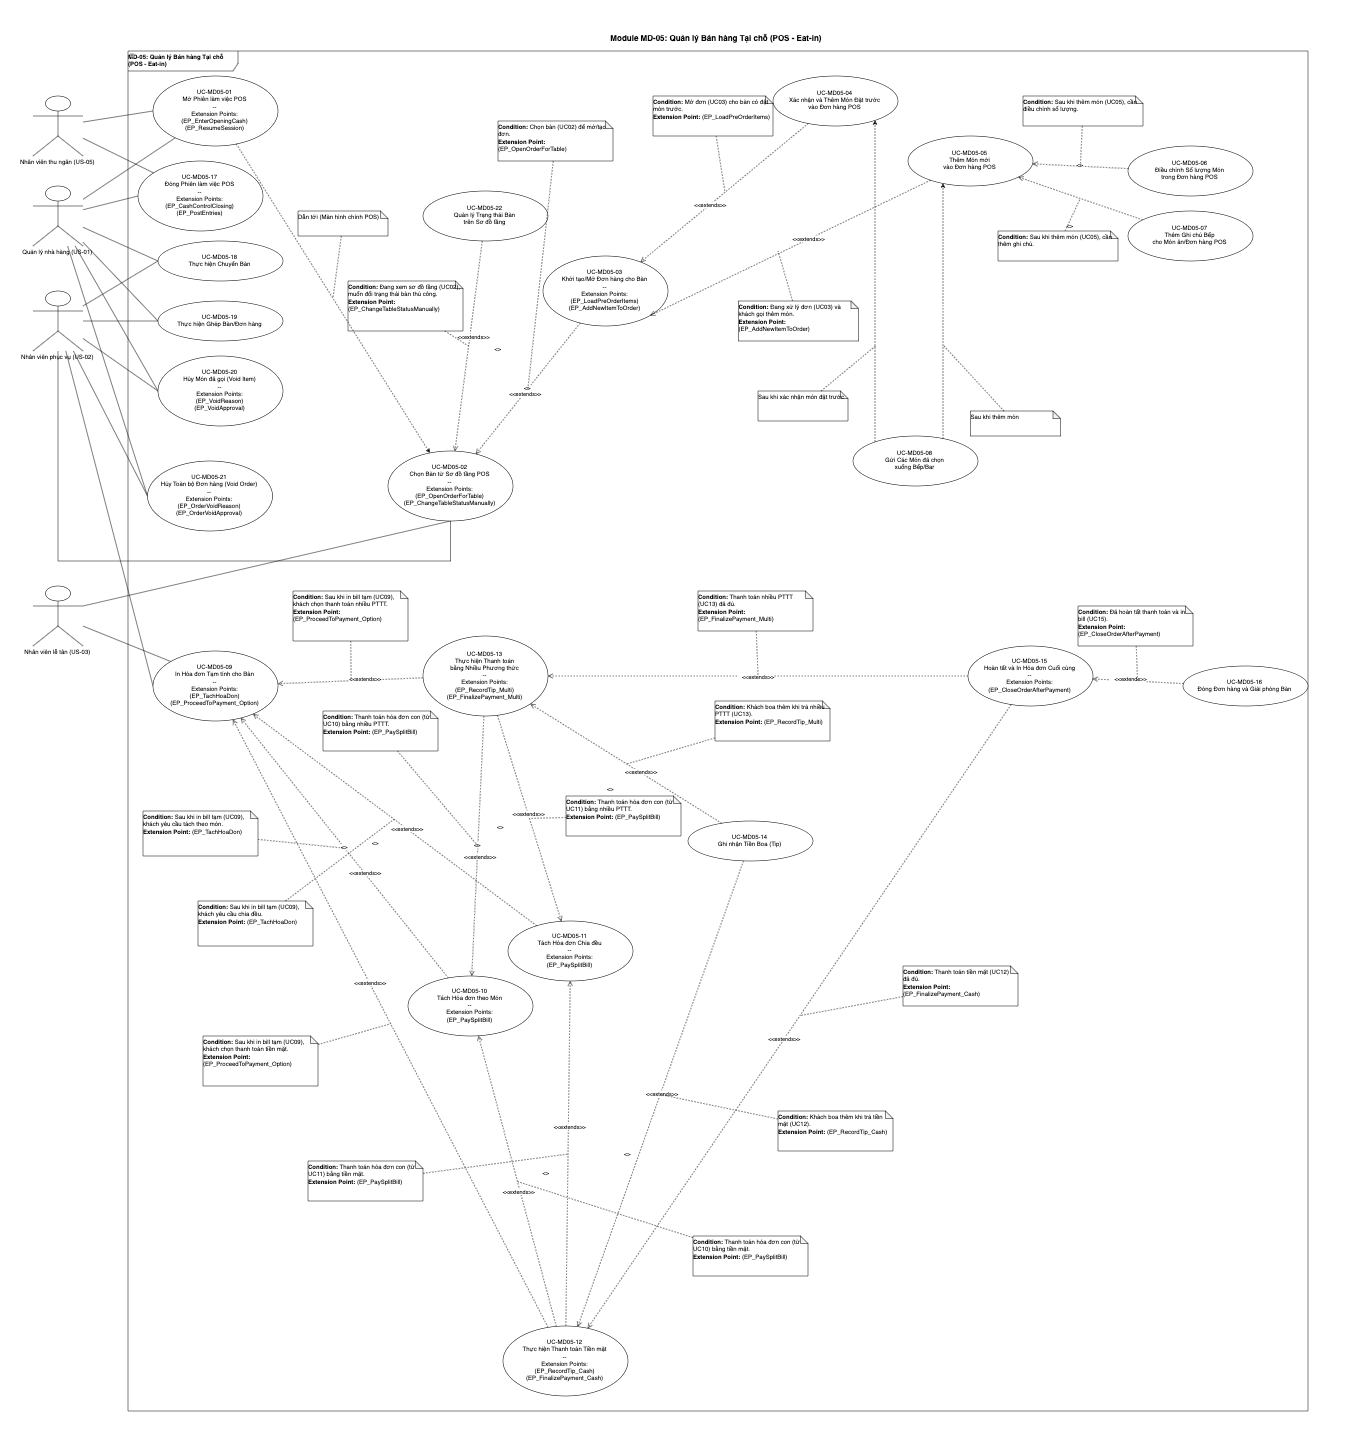
\includegraphics[width=15cm]{Sections/tong_quan/functional_spec/img/uc5.png}
    \vspace{0.5cm}
    \caption{Use case diagram cho Module MD-05}
    \label{fig:my_label}
\end{figure}

\begin{longtable}{|m{2cm}|m{2.5cm}|m{2cm}|m{4.5cm}|m{4cm}|}
\caption{Danh sách Yêu cầu Chức năng cho Module MD-05: Quản lý Bán hàng Tại chỗ (POS - Eat-in)} \label{tab:fr_md05_revised_v3_no_card} \\
\hline
\textbf{Mã Module} & \textbf{Mã Yêu cầu CN} & \textbf{Mã Người dùng} & \textbf{Tên Chức năng} & \textbf{Mô tả Ngắn} \\
\hline
\endhead % Header cho các trang tiếp theo
\hline
\endfoot % Footer cho bảng
\hline
\endlastfoot % Footer cho trang cuối cùng

MD-05 & FR-MD05-01 & US-05/US-01 & Mở Phiên làm việc POS & Cho phép Thu ngân/Quản lý bắt đầu phiên POS, nhập tiền mặt đầu ca. \\
\hline
MD-05 & FR-MD05-02 & US-02/US-03 & Chọn Bàn từ Sơ đồ tầng POS & Nhân viên chọn bàn trống hoặc bàn có khách/đặt trước từ sơ đồ tầng. \\
\hline
MD-05 & FR-MD05-03 & US-02 & Khởi tạo/Mở Đơn hàng cho Bàn & Hệ thống tạo đơn mới cho bàn trống hoặc mở đơn hiện có của bàn đang hoạt động/có đặt trước. \\
\hline
MD-05 & FR-MD05-04 & US-02 & Xác nhận và Thêm Món Đặt trước vào Đơn hàng POS & Nhân viên xem các món khách đã đặt trước (nếu có) và xác nhận thêm vào đơn hàng POS. \\
\hline
MD-05 & FR-MD05-05 & US-02 & Thêm Món mới vào Đơn hàng POS & Nhân viên chọn món từ menu POS để thêm vào đơn hàng hiện tại. \\
\hline
MD-05 & FR-MD05-06 & US-02 & Điều chỉnh Số lượng Món trong Đơn hàng POS & Nhân viên tăng/giảm số lượng một món đã có trong đơn hàng. \\
\hline
MD-05 & FR-MD05-07 & US-02 & Thêm Ghi chú Bếp cho Món ăn/Đơn hàng POS & Nhân viên thêm yêu cầu đặc biệt cho món hoặc cả đơn. \\
\hline
MD-05 & FR-MD05-08 & US-02 & Gửi Các Món đã chọn xuống Bếp/Bar & Nhân viên gửi các món mới thêm/món đặt trước đã xác nhận xuống bộ phận chuẩn bị. \\
\hline
MD-05 & FR-MD05-09 & US-02 & In Hóa đơn Tạm tính cho Bàn & Nhân viên in bill tạm tính (đã trừ cọc nếu có) cho khách kiểm tra. \\
\hline
MD-05 & FR-MD05-10 & US-02 & Tách Hóa đơn theo Món & Nhân viên chia hóa đơn của bàn theo từng món ăn cụ thể. \\
\hline
MD-05 & FR-MD05-11 & US-02 & Tách Hóa đơn Chia đều & Nhân viên chia đều tổng hóa đơn cho một số lượng người/phần nhất định. \\
\hline
MD-05 & FR-MD05-12 & US-02/US-05 & Thực hiện Thanh toán Tiền mặt & Nhân viên nhận tiền mặt, nhập số tiền nhận và hệ thống tính tiền thừa. \\
\hline
% FR-MD05-13 (Thanh toán thẻ) ĐÃ BỊ LOẠI BỎ
% Đánh số lại các FR tiếp theo
MD-05 & FR-MD05-13 & US-02/US-05 & Thực hiện Thanh toán bằng Nhiều Phương thức (Không bao gồm Thẻ) & Nhân viên nhận thanh toán cho một hóa đơn bằng cách kết hợp nhiều phương thức được hỗ trợ (ví dụ: Tiền mặt và Ví điện tử). \\
\hline
MD-05 & FR-MD05-14 & US-02/US-05 & Ghi nhận Tiền Boa (Tip) & Nhân viên nhập số tiền boa khách hàng trả thêm. \\
\hline
MD-05 & FR-MD05-15 & US-02/US-05 & Hoàn tất và In Hóa đơn Cuối cùng & Sau khi nhận đủ tiền, nhân viên xác nhận hoàn tất thanh toán và in hóa đơn/biên lai. \\
\hline
MD-05 & FR-MD05-16 & US-02 & Đóng Đơn hàng và Giải phóng Bàn & Nhân viên đóng đơn hàng đã thanh toán và cập nhật bàn thành trống. \\
\hline
MD-05 & FR-MD05-17 & US-05/US-01 & Đóng Phiên làm việc POS & Thu ngân/Quản lý kết thúc phiên, tổng kết, đối chiếu tiền mặt. \\
\hline
MD-05 & FR-MD05-18 & US-01/US-02 & Thực hiện Chuyển Bàn & Nhân viên chuyển toàn bộ đơn hàng từ bàn này sang bàn trống khác. \\
\hline
MD-05 & FR-MD05-19 & US-01/US-02 & Thực hiện Ghép Bàn/Đơn hàng & Nhân viên gộp nhiều đơn hàng từ các bàn khác nhau vào một bàn. \\
\hline
MD-05 & FR-MD05-20 & US-01/US-02 & Hủy Món đã gọi (Void Item) & Nhân viên hủy một món đã thêm vào đơn (có thể cần quyền). \\
\hline
MD-05 & FR-MD05-21 & US-01/US-02 & Hủy Toàn bộ Đơn hàng (Void Order) & Nhân viên hủy cả đơn hàng đang xử lý (có thể cần quyền). \\
\hline
MD-05 & FR-MD05-22 & US-02/ US-03 & Quản lý Trạng thái Bàn trên Sơ đồ tầng & Nhân viên có thể thay đổi thủ công trạng thái bàn (ví dụ: "Cần dọn", "Đang chờ") nếu cần. \\
\hline

\end{longtable}


\subsubsubsection{Mục tiêu và Phạm vi}
\label{sssec:md05_objectives_scope}
Mục tiêu chính của module MD-05 là:
\begin{itemize}
    \item \textbf{Tối ưu hóa quy trình phục vụ tại bàn:} Cung cấp một giao diện nhanh chóng, trực quan và dễ sử dụng cho nhân viên để nhận đơn, gửi bếp, và quản lý các yêu cầu của khách.
    \item \textbf{Quản lý bàn hiệu quả:} Hiển thị sơ đồ tầng trực quan với trạng thái bàn cập nhật theo thời gian thực, hỗ trợ việc xếp khách và theo dõi tình trạng phục vụ.
    \item \textbf{Đảm bảo tính chính xác của đơn hàng:} Giảm thiểu sai sót trong việc ghi nhận món ăn, số lượng, biến thể, và các yêu cầu đặc biệt của khách.
    \item \textbf{Tích hợp liền mạch với bếp/bar:} Gửi thông tin đơn hàng một cách chính xác và kịp thời đến các bộ phận chuẩn bị thông qua máy in hoặc Màn hình Hiển thị Bếp (KDS).
    \item \textbf{Linh hoạt trong thanh toán:} Hỗ trợ nhiều phương thức thanh toán, khả năng tách hóa đơn, và ghi nhận tiền boa.
    \item \textbf{Kiểm soát và báo cáo tài chính:} Ghi nhận tất cả các giao dịch, hỗ trợ đối chiếu tiền mặt cuối ca và cung cấp dữ liệu cho việc tạo các bút toán kế toán.
    \item \textbf{Nâng cao trải nghiệm khách hàng:} Thông qua việc phục vụ nhanh chóng, chính xác và khả năng đáp ứng linh hoạt các yêu cầu của khách.
\end{itemize}
Phạm vi của module bao gồm toàn bộ các hoạt động từ khi nhân viên mở phiên làm việc POS, quản lý đơn hàng cho từng bàn (tạo mới, thêm/sửa/hủy món, chuyển/ghép bàn), xử lý thanh toán, cho đến khi đóng phiên làm việc và tổng kết doanh thu.

\subsubsubsection{Đối tượng Sử dụng Chính}
\label{sssec:md05_primary_users}
Module này chủ yếu được sử dụng bởi các nhân viên tuyến đầu của nhà hàng:
\begin{itemize}
    \item \textbf{US-02 (Nhân viên phục vụ):} Là người dùng thường xuyên nhất, chịu trách nhiệm chính trong việc sử dụng sơ đồ tầng, nhận đơn hàng từ khách, thêm món, gửi yêu cầu bếp, và có thể cả việc nhận một phần thanh toán.
    \item \textbf{US-05 (Nhân viên thu ngân):} Chịu trách nhiệm mở và đóng phiên làm việc POS, xử lý các giao dịch thanh toán phức tạp, đối chiếu tiền mặt.
    \item \textbf{US-01 (Quản lý nhà hàng):} Có thể thực hiện tất cả các chức năng của nhân viên phục vụ và thu ngân, đồng thời có quyền thực hiện các hành động quản lý như hủy món/đơn hàng, chuyển/ghép bàn, và xem báo cáo phiên.
    \item \textbf{US-03 (Nhân viên lễ tân):} Có thể sử dụng sơ đồ tầng để xếp khách và mở đơn hàng ban đầu cho bàn.
\end{itemize}

\subsubsubsection{Các Chức năng Chính}
\label{sssec:md05_key_functionalities}
Module MD-05 cung cấp một bộ các chức năng toàn diện cho việc bán hàng tại chỗ, được mô tả chi tiết qua các Use Case sau:

\begin{itemize}
    \item \textbf{Quản lý Phiên làm việc POS (UC-MD05-01, UC-MD05-17):}
    \begin{itemize}
        \item Mở một phiên làm việc mới, tùy chọn nhập số dư tiền mặt đầu ca (UC-MD05-01).
        \item Đóng phiên làm việc cuối ca, tổng kết giao dịch, đối chiếu tiền mặt và ghi nhận bút toán (UC-MD05-17).
    \end{itemize}

    \item \textbf{Quản lý Bàn và Đơn hàng (UC-MD05-02, UC-MD05-03, UC-MD05-18, UC-MD05-19, UC-MD05-22):}
    \begin{itemize}
        \item Hiển thị và cho phép chọn bàn từ sơ đồ tầng trực quan với trạng thái cập nhật (UC-MD05-02).
        \item Khởi tạo một đơn hàng mới cho bàn trống/đặt trước hoặc mở lại đơn hàng đang hoạt động của bàn đã có khách (UC-MD05-03).
        \item Thực hiện chuyển toàn bộ đơn hàng từ bàn này sang bàn khác (UC-MD05-18).
        \item Thực hiện ghép các đơn hàng từ nhiều bàn vào một bàn đích duy nhất (UC-MD05-19).
        \item (Tùy chọn) Cho phép nhân viên thay đổi thủ công trạng thái của bàn trên sơ đồ tầng (ví dụ: "Cần dọn dẹp") (UC-MD05-22).
    \end{itemize}

    \item \textbf{Thao tác trên Đơn hàng (UC-MD05-04 đến UC-MD05-08, UC-MD05-20, UC-MD05-21):}
    \begin{itemize}
        \item Tự động tải và cho phép nhân viên xác nhận/thêm các món khách đã đặt trước online vào đơn hàng POS (UC-MD05-04).
        \item Thêm các món ăn/đồ uống mới vào đơn hàng từ menu trực quan, bao gồm cả việc chọn biến thể (UC-MD05-05).
        \item Điều chỉnh số lượng của một món đã có trong đơn hàng (UC-MD05-06).
        \item Thêm các ghi chú hoặc yêu cầu đặc biệt của khách cho từng món hoặc toàn bộ đơn hàng để gửi xuống bếp (UC-MD05-07).
        \item Gửi thông tin các món đã chọn (mới hoặc đặt trước) xuống các máy in bếp/bar hoặc màn hình KDS tương ứng (UC-MD05-08).
        \item Hủy một món cụ thể đã gọi trong đơn hàng (Void Item), có thể yêu cầu lý do và quyền quản lý (UC-MD05-20).
        \item Hủy toàn bộ một đơn hàng đang hoạt động (Void Order), thường yêu cầu quyền quản lý và lý do (UC-MD05-21).
    \end{itemize}

    \item \textbf{Xử lý Thanh toán (UC-MD05-09 đến UC-MD05-16):}
    \begin{itemize}
        \item In hóa đơn tạm tính cho khách kiểm tra, bao gồm cả việc trừ tiền đặt cọc đã thanh toán (nếu có) (UC-MD05-09).
        \item Tách hóa đơn theo từng món ăn cụ thể để nhiều người có thể trả riêng (UC-MD05-10).
        \item Tách hóa đơn bằng cách chia đều tổng giá trị cho một số lượng người nhất định (UC-MD05-11).
        \item Thực hiện thanh toán bằng tiền mặt, tính toán tiền trả lại (UC-MD05-12).
        \item Thực hiện thanh toán bằng nhiều phương thức khác nhau (không bao gồm thẻ tích hợp terminal) cho cùng một hóa đơn (UC-MD05-13).
        \item Ghi nhận số tiền boa (tip) do khách hàng trả thêm (UC-MD05-14).
        \item Sau khi nhận đủ thanh toán, hoàn tất giao dịch và in hóa đơn/biên lai cuối cùng cho khách (UC-MD05-15).
        \item Đóng đơn hàng đã thanh toán và giải phóng bàn, cập nhật trạng thái bàn thành trống (UC-MD05-16).
    \end{itemize}
\end{itemize}

\subsubsubsection{Tóm tắt Luồng Hoạt động Tổng thể}
\label{sssec:md05_overall_workflow}
Luồng hoạt động chính trong module Bán hàng Tại chỗ (POS) thường diễn ra như sau:
\begin{enumerate}
    \item \textbf{Bắt đầu ca làm việc:} Nhân viên thu ngân/Quản lý Mở Phiên làm việc POS (UC-MD05-01), nhập số dư tiền mặt đầu ca nếu cần.
    \item \textbf{Chọn bàn và mở đơn hàng:}
        \begin{itemize}
            \item Nhân viên phục vụ Chọn Bàn từ Sơ đồ tầng POS (UC-MD05-02) dựa trên tình trạng bàn (trống, đặt trước).
            \item Hệ thống Khởi tạo/Mở Đơn hàng cho Bàn (UC-MD05-03).
        \end{itemize}
    \item \textbf{Nhận yêu cầu gọi món từ khách:}
        \begin{itemize}
            \item Nếu bàn có đặt món trước, nhân viên Xác nhận và Thêm Món Đặt trước vào Đơn hàng POS (UC-MD05-04).
            \item Nhân viên Thêm Món mới vào Đơn hàng POS (UC-MD05-05) theo yêu cầu của khách.
            \item Điều chỉnh Số lượng Món (UC-MD05-06) hoặc Thêm Ghi chú Bếp (UC-MD05-07) nếu cần.
            \item Sau mỗi lượt gọi món hoặc khi cần, nhân viên Gửi Các Món đã chọn xuống Bếp/Bar (UC-MD05-08).
        \end{itemize}
    \item \textbf{Quản lý đơn hàng trong quá trình phục vụ (nếu có):}
        \begin{itemize}
            \item Khách yêu cầu chuyển bàn: Nhân viên Thực hiện Chuyển Bàn (UC-MD05-18).
            \item Nhiều nhóm khách muốn ngồi chung: Nhân viên Thực hiện Ghép Bàn/Đơn hàng (UC-MD05-19).
            \item Khách đổi ý/nhân viên nhập sai: Nhân viên Hủy Món đã gọi (Void Item) (UC-MD05-20).
            \item Khách rời đi/lỗi nghiêm trọng: Nhân viên/Quản lý Hủy Toàn bộ Đơn hàng (Void Order) (UC-MD05-21).
            \item Cập nhật trạng thái bàn thủ công (ví dụ: "Cần dọn"): Nhân viên Quản lý Trạng thái Bàn trên Sơ đồ tầng (UC-MD05-22).
        \end{itemize}
    \item \textbf{Khách yêu cầu thanh toán:}
        \begin{itemize}
            \item Nhân viên In Hóa đơn Tạm tính cho Bàn (UC-MD05-09).
            \item Nếu khách yêu cầu trả riêng: Nhân viên Tách Hóa đơn theo Món (UC-MD05-10) hoặc Tách Hóa đơn Chia đều (UC-MD05-11).
            \item Nhân viên nhận thanh toán bằng các phương thức: Thực hiện Thanh toán Tiền mặt (UC-MD05-12), hoặc Thực hiện Thanh toán bằng Nhiều Phương thức (UC-MD05-13).
            \item Nếu khách boa: Nhân viên Ghi nhận Tiền Boa (Tip) (UC-MD05-14).
        \end{itemize}
    \item \textbf{Hoàn tất giao dịch:}
        \begin{itemize}
            \item Sau khi nhận đủ tiền, nhân viên Hoàn tất và In Hóa đơn Cuối cùng (UC-MD05-15).
            \item Cuối cùng, nhân viên Đóng Đơn hàng và Giải phóng Bàn (UC-MD05-16).
        \end{itemize}
    \item \textbf{Kết thúc ca làm việc:} Nhân viên thu ngân/Quản lý Đóng Phiên làm việc POS (UC-MD05-17), tổng kết và đối chiếu.
\end{enumerate}
Module MD-05 là trung tâm của các hoạt động dịch vụ tại nhà hàng, đảm bảo quy trình diễn ra mượt mà, chính xác và hiệu quả.

\subsubsection{Module MD-06: Quản lý Bán mang về (POS - Takeout)}

\begin{longtable}{|m{2cm}|m{2.5cm}|m{2.5cm}|m{4.5cm}|m{4cm}|}
\caption{Danh sách Yêu cầu Chức năng cho Module MD-06: Quản lý Bán mang về (POS - Takeout)} \label{tab:fr_md06} \\
\hline
\textbf{Mã Module} & \textbf{Mã Yêu cầu CN} & \textbf{Mã Người dùng} & \textbf{Tên Chức năng} & \textbf{Mô tả Ngắn} \\
\hline
\endhead % Header cho các trang tiếp theo

\hline
\endfoot % Footer cho bảng

\hline
\endlastfoot % Footer cho trang cuối cùng

MD-06 & FR-MD06-01 & US-02, US-05 & Chọn Chế độ Bán Mang về & Cho phép nhân viên chọn một chế độ/giao diện riêng biệt trên POS dành cho việc tạo đơn hàng mang về, bỏ qua bước chọn bàn. \\
\hline
MD-06 & FR-MD06-02 & US-02, US-05 & Tạo Đơn hàng Mang về & Khởi tạo một đơn hàng mới trong chế độ mang về, không liên kết với bàn cụ thể. \\
\hline
MD-06 & FR-MD06-03 & US-02, US-05 & (Tùy chọn) Liên kết Khách hàng & Cho phép tìm kiếm và liên kết đơn hàng mang về với một khách hàng đã có trong hệ thống hoặc tạo nhanh thông tin khách hàng mới (Tên, SĐT). \\
\hline
MD-06 & FR-MD06-04 & US-02, US-05 & Thêm món vào Đơn hàng Mang về & Cho phép nhân viên thêm các món ăn/đồ uống vào đơn hàng mang về, tương tự như cách thêm món cho đơn hàng tại bàn (UC-MD05-05). \\
\hline
MD-06 & FR-MD06-05 & US-02, US-05 & Xử lý Ghi chú cho Đơn Mang về & Cho phép thêm ghi chú đặc biệt cho các món hoặc toàn bộ đơn hàng mang về (ví dụ: "Gói kỹ", "Thêm tương ớt"). Tương tự UC-MD05-06. \\
\hline
MD-06 & FR-MD06-06 & US-02, US-05 & Gửi đơn Mang về xuống Bếp/Bar & Gửi thông tin các món cần chuẩn bị cho đơn hàng mang về đến các bộ phận liên quan (Bếp/Bar). Tương tự UC-MD05-07, có thể cần đánh dấu là đơn "Takeout". \\
\hline
MD-06 & FR-MD06-07 & US-02, US-05, System & Áp dụng Đặt cọc (Nếu Đặt trước Online) & Nếu đơn hàng mang về này được khách đặt trước online (qua một luồng khác) và có đặt cọc, hệ thống cần áp dụng tiền cọc vào hóa đơn. (Logic tương tự UC-MD05-09 nhưng áp dụng cho đơn takeout). \\
\hline
MD-06 & FR-MD06-08 & US-02, US-05 & Thanh toán Đơn hàng Mang về & Cho phép nhận thanh toán ngay tại quầy cho đơn hàng mang về bằng các phương thức khác nhau. Tương tự UC-MD05-11. \\
\hline
MD-06 & FR-MD06-09 & US-02, US-05 & In Hóa đơn/Phiếu thu Mang về & In hóa đơn/phiếu thu cho khách hàng sau khi thanh toán thành công. Có thể cần mẫu in khác biệt cho đơn mang về. \\
\hline
MD-06 & FR-MD06-10 & US-02, US-05 & Đóng Đơn hàng Mang về & Hoàn tất và đóng đơn hàng mang về sau khi khách đã thanh toán và nhận hàng. \\
\hline

\end{longtable}

\subsubsection{Module MD-07: Quản lý Giao hàng (POS - Delivery)}
Module Quản lý Giao hàng (MD-07) là một thành phần quan trọng của hệ thống Point of Sale (POS), được thiết kế đặc biệt để hỗ trợ nhà hàng quản lý các đơn hàng mà khách yêu cầu giao đến một địa chỉ cụ thể. Module này tập trung vào việc thu thập thông tin khách hàng và địa chỉ giao hàng, xử lý đơn hàng, và đặc biệt là tích hợp với dịch vụ quản lý giao hàng của bên thứ ba (trong trường hợp này là Shipday) để tự động hóa việc gửi yêu cầu giao hàng và theo dõi trạng thái.



\begin{figure}[H]
    \centering
    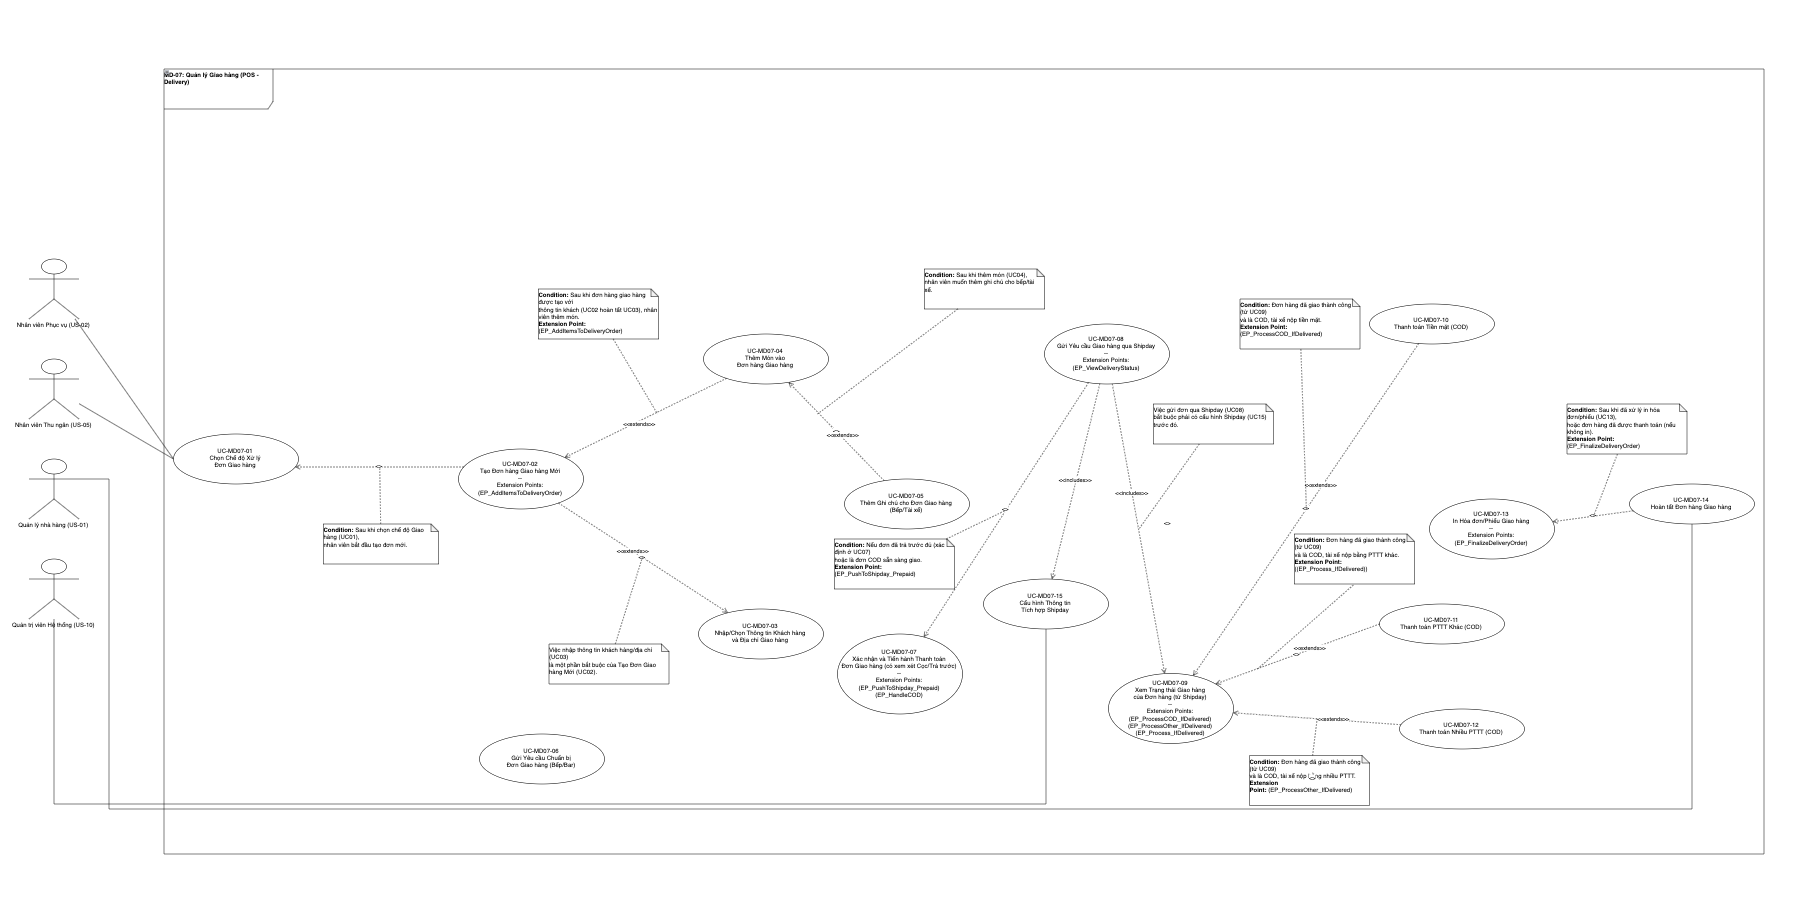
\includegraphics[width=15cm]{Sections/tong_quan/functional_spec/img/uc7.png}
    \vspace{0.5cm}
    \caption{Use case diagram cho Module MD-07}
    \label{fig:my_label}
\end{figure}

\begin{longtable}{|m{2cm}|m{2.5cm}|m{2.5cm}|m{4.5cm}|m{4cm}|}
\caption{Danh sách Yêu cầu Chức năng cho Module MD-07: Quản lý Giao hàng (POS - Delivery)} \label{tab:fr_md07_revised_v2} \\
\hline
\textbf{Mã Module} & \textbf{Mã Yêu cầu CN} & \textbf{Mã Người dùng} & \textbf{Tên Chức năng} & \textbf{Mô tả Ngắn} \\
\hline
\endhead % Header cho các trang tiếp theo
\hline
\endfoot % Footer cho bảng
\hline
\endlastfoot % Footer cho trang cuối cùng

MD-07 & FR-MD07-01 & US-02, US-05 & Chọn Chế độ Xử lý Đơn Giao hàng & Nhân viên chọn chế độ/giao diện riêng trên POS cho đơn giao hàng. \\
\hline
MD-07 & FR-MD07-02 & US-02, US-05 & Tạo Đơn hàng Giao hàng Mới & Nhân viên khởi tạo đơn hàng mới, yêu cầu liên kết thông tin khách hàng giao hàng. \\
\hline
MD-07 & FR-MD07-03 & US-02, US-05 & Nhập/Chọn Thông tin Khách hàng và Địa chỉ Giao hàng & Nhân viên tìm/chọn khách hàng có sẵn hoặc nhập mới Tên, SĐT, Địa chỉ giao hàng chi tiết. \\
\hline
MD-07 & FR-MD07-04 & US-02, US-05 & Thêm Món vào Đơn hàng Giao hàng & Nhân viên thêm món ăn/đồ uống vào đơn hàng giao đi. \\
\hline
MD-07 & FR-MD07-05 & US-02, US-05 & Thêm Ghi chú cho Đơn Giao hàng (Bếp/Tài xế) & Nhân viên thêm ghi chú cho bếp hoặc ghi chú cho tài xế giao hàng. \\
\hline
MD-07 & FR-MD07-06 & US-02, US-05 & Gửi Yêu cầu Chuẩn bị Đơn Giao hàng (Bếp/Bar) & Nhân viên gửi thông tin món cần chuẩn bị xuống bếp/bar, có đánh dấu "Delivery". \\
\hline
MD-07 & FR-MD07-07 & US-02, US-05 & Xác nhận và Tiến hành Thanh toán Đơn Giao hàng (có xem xét Cọc/Trả trước) & Nhân viên vào màn hình thanh toán, nơi hệ thống đã tự động áp dụng cọc/trả trước (nếu đơn hàng được đặt online và có trả trước). \\
\hline
MD-07 & FR-MD07-08 & US-02, US-05 & Gửi Yêu cầu Giao hàng qua Shipday & Sau khi đơn hàng sẵn sàng, nhân viên kích hoạt gửi thông tin đơn hàng sang Shipday. \\
\hline
MD-07 & FR-MD07-09 & US-02, US-05, US-01 & Xem Trạng thái Giao hàng của Đơn hàng (từ Shipday) & Nhân viên xem trạng thái giao hàng (Đã gán tài xế, Đang giao...) được cập nhật từ Shipday trên chi tiết đơn hàng. \\
\hline
MD-07 & FR-MD07-10 & US-02, US-05 & Thực hiện Thanh toán Tiền mặt cho Đơn Giao hàng (Nếu COD) & Nhân viên nhận tiền mặt COD từ tài xế và ghi nhận vào hệ thống. \\
\hline
MD-07 & FR-MD07-11 & US-02, US-05 & Ghi nhận Thanh toán bằng Phương thức Khác (Không Thẻ) cho Đơn Giao hàng (Nếu COD) & Nhân viên ghi nhận thanh toán COD bằng phương thức khác được hỗ trợ. \\
\hline
MD-07 & FR-MD07-12 & US-02, US-05 & Thực hiện Thanh toán Đơn Giao hàng bằng Nhiều Phương thức (Không Thẻ, Nếu COD) & Nhân viên nhận thanh toán COD bằng nhiều phương thức. \\
\hline
MD-07 & FR-MD07-13 & US-02, US-05 & In Hóa đơn/Phiếu Giao hàng & Nhân viên in hóa đơn/phiếu giao hàng để tài xế sử dụng. \\
\hline
MD-07 & FR-MD07-14 & US-02, US-05 & Hoàn tất Đơn hàng Giao hàng & Nhân viên đóng đơn hàng giao đi sau khi đã giao thành công và (nếu COD) đã nhận đủ thanh toán. \\
\hline
MD-07 & FR-MD07-15 & US-01/US-10 & Cấu hình Thông tin Tích hợp Shipday & Quản trị viên/Quản lý cấu hình các tham số kết nối API và Shipday. \\
\hline

\end{longtable}


\subsubsubsection{Mục tiêu và Phạm vi}
\label{sssec:md07_objectives_scope}
Mục tiêu chính của module MD-07 bao gồm:
\begin{itemize}
    \item \textbf{Quản lý hiệu quả đơn hàng giao đi:} Cung cấp một quy trình đầy đủ từ việc nhận đơn, nhập thông tin khách hàng và địa chỉ, xử lý món ăn, cho đến khi gửi đơn cho đơn vị vận chuyển và theo dõi.
    \item \textbf{Tích hợp liền mạch với dịch vụ giao hàng bên ngoài (Shipday):} Tự động hóa việc gửi thông tin đơn hàng sang Shipday để tìm tài xế và quản lý quá trình giao hàng.
    \item \textbf{Theo dõi trạng thái giao hàng:} Cập nhật trạng thái đơn hàng trong hệ thống dựa trên thông tin phản hồi từ Shipday.
    \item \textbf{Xử lý thanh toán linh hoạt cho đơn giao hàng:} Hỗ trợ các hình thức thanh toán như trả trước online hoặc thu tiền khi nhận hàng (COD).
    \item \textbf{Cung cấp thông tin chính xác cho các bên liên quan:} Đảm bảo bếp/bar nhận đúng yêu cầu chuẩn bị, tài xế có đủ thông tin giao hàng, và nhân viên nhà hàng có thể theo dõi quá trình.
    \item \textbf{Nâng cao trải nghiệm khách hàng:} Thông qua việc giao hàng đúng hẹn và thông tin rõ ràng.
\end{itemize}
Phạm vi của module bao gồm từ việc nhân viên chọn chế độ xử lý đơn giao hàng, tạo đơn hàng, nhập thông tin chi tiết, gửi yêu cầu chuẩn bị, gửi đơn sang Shipday, theo dõi trạng thái, cho đến khi xử lý thanh toán COD (nếu có) và hoàn tất đơn hàng.

\subsubsubsection{Đối tượng Sử dụng Chính}
\label{sssec:md07_primary_users}
Các đối tượng người dùng và hệ thống chính tương tác với module này bao gồm:
\begin{itemize}
    \item \textbf{US-02 (Nhân viên phục vụ) / US-05 (Nhân viên thu ngân):} Là những người trực tiếp nhận yêu cầu đặt hàng giao đi, tạo đơn hàng trên POS, nhập thông tin khách hàng, địa chỉ, món ăn, và gửi yêu cầu giao hàng sang Shipday.
    \item \textbf{US-01 (Quản lý nhà hàng):} Có thể thực hiện tất cả các chức năng của nhân viên, giám sát quá trình, xử lý các trường hợp đặc biệt, và cấu hình tích hợp.
    \item \textbf{US-10 (Quản trị viên Hệ thống):} Chịu trách nhiệm cấu hình kỹ thuật cho việc tích hợp API với Shipday.
    \item \textbf{System (Hệ thống Shipday):} Hệ thống tự động hóa nhiều bước, trong khi Shipday là hệ thống bên ngoài chịu trách nhiệm quản lý đội xe và quá trình giao hàng thực tế.
\end{itemize}

\subsubsubsection{Các Chức năng Chính}
\label{sssec:md07_key_functionalities}
Module MD-07 cung cấp một chuỗi các chức năng để quản lý toàn diện quy trình giao hàng, được mô tả chi tiết qua các Use Case sau:

\begin{itemize}
    \item \textbf{Khởi tạo và Chuẩn bị Đơn hàng Giao hàng (UC-MD07-01 đến UC-MD07-06):}
    \begin{itemize}
        \item Cho phép nhân viên chọn chế độ hoạt động hoặc giao diện dành riêng cho việc xử lý đơn hàng giao đi (UC-MD07-01).
        \item Nhân viên khởi tạo một đơn hàng POS mới, được hệ thống tự động đánh dấu là loại hình "Giao hàng" (UC-MD07-02).
        \item Yêu cầu nhân viên bắt buộc phải nhập hoặc chọn thông tin khách hàng và địa chỉ giao hàng chi tiết cho đơn hàng (UC-MD07-03).
        \item Thêm các món ăn/đồ uống từ thực đơn POS vào đơn hàng giao đi (UC-MD07-04, tương tự UC-MD05-05).
        \item Thêm các ghi chú đặc biệt cho bếp (về món ăn) hoặc cho tài xế (về việc giao hàng) (UC-MD07-05, tương tự UC-MD05-07 nhưng có thêm ghi chú cho tài xế).
        \item Gửi thông tin các món cần chuẩn bị của đơn hàng giao đi xuống các máy in bếp/bar hoặc màn hình KDS, có chỉ dẫn rõ là đơn "Delivery" (UC-MD07-06, tương tự UC-MD05-08 nhưng có thêm thông tin "Delivery").
    \end{itemize}

    \item \textbf{Xử lý Thanh toán và Tích hợp Giao hàng (UC-MD07-07, UC-MD07-08, UC-MD07-10, UC-MD07-11, UC-MD07-12):}
    \begin{itemize}
        \item Trước khi vào màn hình thanh toán hoặc xác nhận đơn, hệ thống tự động kiểm tra và áp dụng (trừ đi) các khoản tiền đặt cọc hoặc thanh toán trước (nếu có) cho đơn hàng giao đi (UC-MD07-07).
        \item Gửi thông tin chi tiết của đơn hàng (bao gồm địa chỉ, thông tin khách, món ăn, số tiền COD nếu có) đến hệ thống quản lý giao hàng Shipday thông qua API (UC-MD07-08).
        \item Đối với đơn hàng COD, cho phép nhân viên ghi nhận việc đã nhận tiền mặt từ tài xế (UC-MD07-10, tương tự UC-MD05-12).
        \item Ghi nhận việc tài xế nộp tiền COD bằng các phương thức khác tiền mặt (ví dụ: chuyển khoản) (UC-MD07-11, tương tự UC-MD06-09 cho Takeout).
        \item (Tùy chọn) Ghi nhận việc tài xế nộp tiền COD bằng nhiều phương thức kết hợp (UC-MD07-12, tương tự UC-MD05-14).
    \end{itemize}

    \item \textbf{Theo dõi và Hoàn tất Đơn hàng Giao hàng (UC-MD07-09, UC-MD07-13, UC-MD07-14):}
    \begin{itemize}
        \item Hiển thị trạng thái giao hàng mới nhất của đơn hàng (ví dụ: "Đang giao", "Đã giao thành công") được hệ thống tự động cập nhật từ Shipday (thường qua webhook) (UC-MD07-09).
        \item In hóa đơn hoặc phiếu giao hàng chi tiết cho đơn hàng giao đi, để đính kèm gói hàng hoặc giao cho khách (UC-MD07-13, tương tự UC-MD06-11).
        \item Chính thức đóng đơn hàng giao đi trong hệ thống sau khi đã xác nhận giao hàng thành công và tất cả các vấn đề thanh toán đã được xử lý (UC-MD07-14, tương tự UC-MD06-12).
    \end{itemize}

    \item \textbf{Cấu hình Tích hợp (UC-MD07-15):}
    \begin{itemize}
        \item Cho phép Quản lý/Quản trị viên thiết lập và quản lý các tham số cần thiết để kết nối và trao đổi dữ liệu với nền tảng Shipday, bao gồm API Key (UC-MD07-15).
    \end{itemize}
\end{itemize}

\subsubsubsection{Tóm tắt Luồng Hoạt động Tổng thể}
\label{sssec:md07_overall_workflow}
Luồng hoạt động chính trong module Quản lý Giao hàng (POS - Delivery) thường diễn ra như sau:
\begin{enumerate}
    \item \textbf{Cấu hình ban đầu:} Quản lý/Quản trị viên Cấu hình Thông tin Tích hợp Shipday (UC-MD07-15).
    \item \textbf{Nhận và tạo đơn hàng giao đi:}
        \begin{itemize}
            \item Nhân viên Chọn Chế độ Xử lý Đơn Giao hàng (UC-MD07-01).
            \item Hệ thống yêu cầu, và nhân viên Tạo Đơn hàng Giao hàng Mới kèm theo việc Nhập/Chọn Thông tin Khách hàng và Địa chỉ Giao hàng (UC-MD07-02, UC-MD07-03).
            \item Nhân viên Thêm Món vào Đơn hàng Giao hàng (UC-MD07-04) và Thêm Ghi chú cho Đơn Giao hàng (Bếp/Tài xế) (UC-MD07-05).
            \item Nhân viên Gửi Yêu cầu Chuẩn bị Đơn Giao hàng (Bếp/Bar) (UC-MD07-06).
        \end{itemize}
    \item \textbf{Xử lý thanh toán và gửi giao hàng:}
        \begin{itemize}
            \item Nhân viên tiến hành xác nhận đơn, hệ thống tự động xem xét và áp dụng các khoản Cọc/Trả trước (UC-MD07-07).
            \item Sau khi đơn hàng sẵn sàng (đã chuẩn bị, thông tin thanh toán rõ ràng), nhân viên Gửi Yêu cầu Giao hàng qua Shipday (UC-MD07-08).
        \end{itemize}
    \item \textbf{Theo dõi và hoàn tất:}
        \begin{itemize}
            \item Nhân viên có thể Xem Trạng thái Giao hàng của Đơn hàng (từ Shipday) (UC-MD07-09) được cập nhật tự động.
            \item Khi cần, nhân viên In Hóa đơn/Phiếu Giao hàng (UC-MD07-13).
            \item Nếu là đơn COD và đã giao thành công, nhân viên ghi nhận thanh toán từ tài xế: Tiền mặt (UC-MD07-10), Phương thức Khác (UC-MD07-11), hoặc Nhiều Phương thức (UC-MD07-12).
            \item Cuối cùng, sau khi giao thành công và thanh toán hoàn tất, nhân viên hoặc hệ thống Hoàn tất Đơn hàng Giao hàng (UC-MD07-14).
        \end{itemize}
\end{enumerate}
Module MD-07 kết hợp các chức năng POS nội bộ với khả năng tích hợp mạnh mẽ của Shipday, tạo nên một giải pháp toàn diện cho việc quản lý dịch vụ giao hàng của nhà hàng.


\subsubsection{Module MD-08: Tích hợp Bếp (Kitchen Integration)}
Module Quản lý Giao hàng (MD-07) là một thành phần quan trọng của hệ thống Point of Sale (POS), được thiết kế đặc biệt để hỗ trợ nhà hàng quản lý các đơn hàng mà khách yêu cầu giao đến một địa chỉ cụ thể. Module này tập trung vào việc thu thập thông tin khách hàng và địa chỉ giao hàng, xử lý đơn hàng, và đặc biệt là tích hợp với dịch vụ quản lý giao hàng của bên thứ ba (trong trường hợp này là Shipday) để tự động hóa việc gửi yêu cầu giao hàng và theo dõi trạng thái.

Module Tích hợp Bếp (MD-08) đóng vai trò cầu nối quan trọng giữa bộ phận phục vụ (thông qua hệ thống POS) và bộ phận bếp/bar. Mục tiêu chính của module này là đảm bảo thông tin đơn hàng được truyền tải một cách chính xác, kịp thời và hiệu quả đến các nhân viên bếp, giúp họ chuẩn bị món ăn đúng theo yêu cầu và tối ưu hóa quy trình làm việc trong bếp. Module này có thể được triển khai dưới dạng Màn hình Hiển thị Bếp (Kitchen Display System - KDS) hoặc thông qua việc sử dụng máy in bếp truyền thống.


\begin{figure}[H]
    \centering
    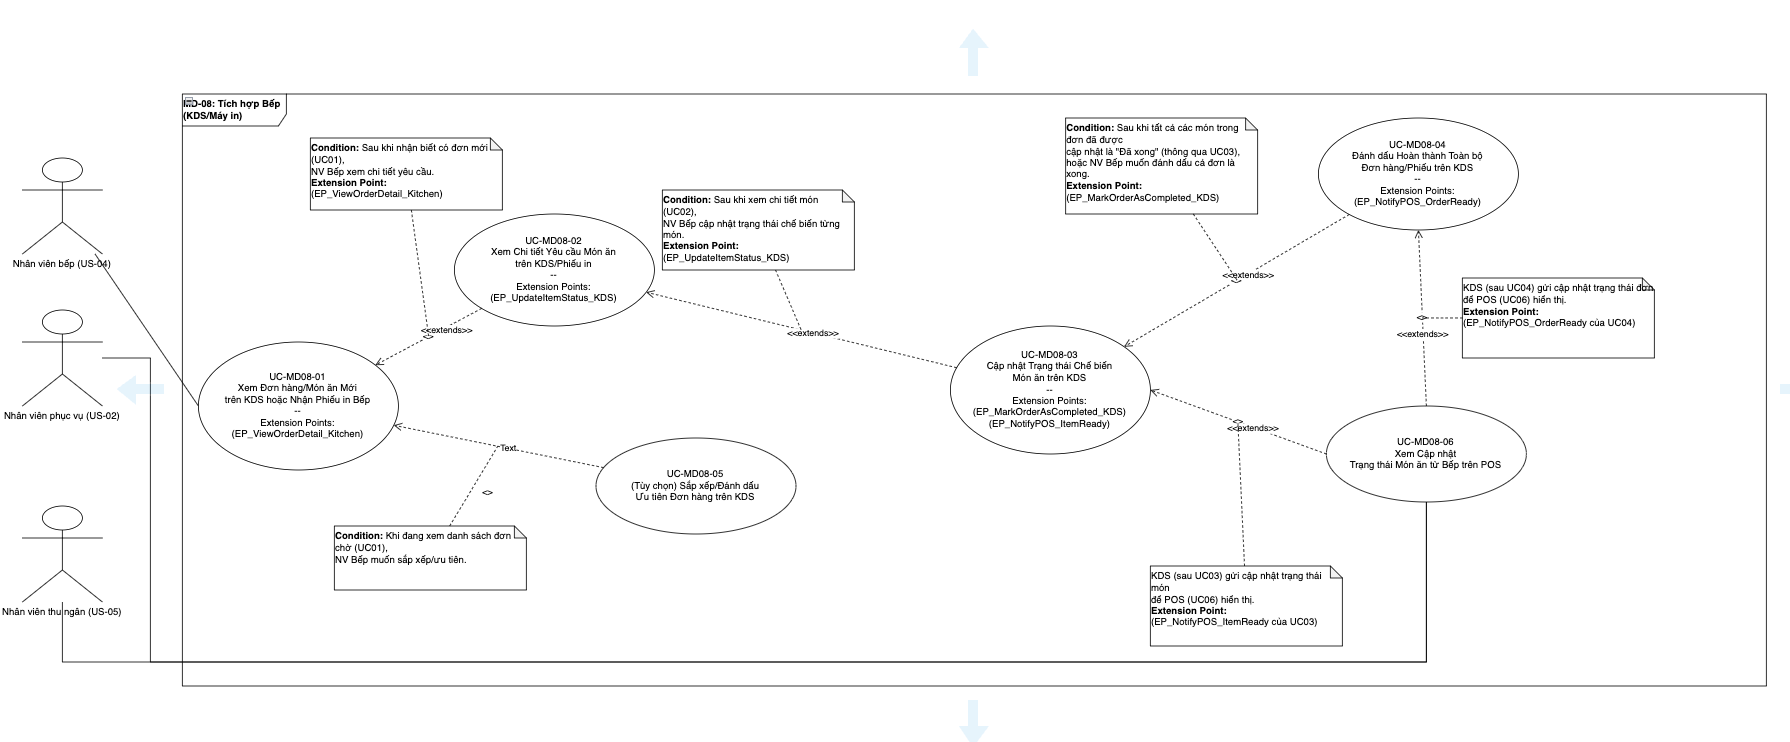
\includegraphics[width=15cm]{Sections/tong_quan/functional_spec/img/uc8.png}
    \vspace{0.5cm}
    \caption{Use case diagram cho Module MD-08}
    \label{fig:my_label}
\end{figure}

\begin{longtable}{|m{2cm}|m{2.5cm}|m{2.5cm}|m{4.5cm}|m{4cm}|}
\caption{Danh sách Yêu cầu Chức năng cho Module MD-08: Tích hợp Bếp (Kitchen Integration)} \label{tab:fr_md08_revised_v2} \\
\hline
\textbf{Mã Module} & \textbf{Mã Yêu cầu CN} & \textbf{Mã Người dùng} & \textbf{Tên Chức năng} & \textbf{Mô tả Ngắn} \\
\hline
\endhead % Header cho các trang tiếp theo
\hline
\endfoot % Footer cho bảng
\hline
\endlastfoot % Footer cho trang cuối cùng

MD-08 & FR-MD08-01 & US-04 & Xem Đơn hàng/Món ăn Mới trên KDS/Máy in Bếp & Nhân viên bếp xem các đơn hàng/món ăn mới được gửi đến KDS hoặc nhận phiếu in từ máy in bếp. (Việc gửi đi là kết quả của FR-MD05-08, FR-MD06-06, FR-MD07-06). \\
\hline
MD-08 & FR-MD08-02 & US-04 & Xem Chi tiết Yêu cầu Món ăn trên KDS/Phiếu in & Nhân viên bếp đọc thông tin chi tiết của từng món cần chuẩn bị: tên, số lượng, biến thể, ghi chú đặc biệt. \\
\hline
MD-08 & FR-MD08-03 & US-04 & Cập nhật Trạng thái Chế biến Món ăn trên KDS & Nhân viên bếp tương tác với KDS để đánh dấu trạng thái chế biến của món ăn (ví dụ: Bắt đầu làm, Đã xong). \\
\hline
MD-08 & FR-MD08-04 & US-04 & Đánh dấu Hoàn thành Toàn bộ Đơn hàng/Phiếu trên KDS & Nhân viên bếp đánh dấu toàn bộ các món trong một đơn hàng/phiếu đã được chuẩn bị xong trên KDS. \\
\hline
MD-08 & FR-MD08-05 & US-04 & Sắp xếp/Đánh dấu Ưu tiên Đơn hàng trên KDS & Nhân viên bếp thay đổi thứ tự hoặc đánh dấu ưu tiên cho các đơn hàng/phiếu trên KDS. \\
\hline
MD-08 & FR-MD08-06 & US-02/US-05 & Xem Cập nhật Trạng thái Món ăn từ Bếp trên POS & Nhân viên phục vụ/thu ngân xem được thông tin món nào đã sẵn sàng từ bếp (nếu KDS có gửi cập nhật về POS). \\
\hline

\end{longtable}


\subsubsubsection{Mục tiêu và Phạm vi}
\label{sssec:md08_objectives_scope}
Mục tiêu chính của module MD-08 là:
\begin{itemize}
    \item \textbf{Truyền tải chính xác yêu cầu món ăn:} Đảm bảo mọi chi tiết của đơn hàng (tên món, số lượng, biến thể, ghi chú đặc biệt) được gửi từ POS đến bếp một cách đầy đủ và không sai sót.
    \item \textbf{Tối ưu hóa quy trình làm việc trong bếp:} Giúp nhân viên bếp dễ dàng tiếp nhận, xem, quản lý và theo dõi tiến độ chuẩn bị các món ăn.
    \item \textbf{Giảm thiểu sai sót và nhầm lẫn:} Hạn chế việc trao đổi thông tin bằng miệng hoặc giấy tờ dễ thất lạc, từ đó giảm lỗi trong quá trình chế biến.
    \item \textbf{Cải thiện thời gian phục vụ:} Giúp bếp nhận yêu cầu nhanh hơn và quản lý thứ tự ưu tiên hiệu quả hơn (đặc biệt với KDS).
    \item \textbf{(Nếu dùng KDS) Cung cấp khả năng theo dõi và cập nhật trạng thái:} Cho phép nhân viên bếp đánh dấu trạng thái chế biến (đang làm, đã xong) và (tùy chọn) đồng bộ thông tin này ngược lại cho nhân viên phục vụ.
    \item \textbf{Hỗ trợ định tuyến thông minh:} Đảm bảo các món ăn được gửi đến đúng trạm chuẩn bị (ví dụ: món chính gửi bếp chính, đồ uống gửi quầy bar) nếu nhà hàng có nhiều khu vực bếp/bar.
\end{itemize}
Phạm vi của module bao gồm việc tiếp nhận yêu cầu món ăn từ hệ thống POS (MD-05, MD-06, MD-07), hiển thị thông tin chi tiết cho nhân viên bếp, và (nếu sử dụng KDS) cho phép nhân viên bếp tương tác để cập nhật trạng thái chế biến. Nó không bao gồm việc quản lý công thức, định lượng nguyên vật liệu, hay các chức năng quản lý kho chi tiết (thuộc các module khác).

\subsubsubsection{Đối tượng Sử dụng Chính}
\label{sssec:md08_primary_users}
Đối tượng người dùng chính của module này là:
\begin{itemize}
    \item \textbf{US-04 (Nhân viên bếp):} Là người trực tiếp sử dụng KDS hoặc nhận phiếu in từ máy in bếp để xem yêu cầu, chuẩn bị món ăn, và (nếu có KDS) cập nhật trạng thái chế biến.
\end{itemize}
Các đối tượng khác tương tác gián tiếp:
\begin{itemize}
    \item \textbf{US-02 (Nhân viên phục vụ) / US-05 (Nhân viên thu ngân):} Là người gửi yêu cầu chuẩn bị món từ POS. Họ cũng có thể (tùy chọn) nhận được cập nhật trạng thái món ăn từ KDS (UC-MD08-06).
    \item \textbf{US-01 (Quản lý nhà hàng) / US-10 (Quản trị viên Hệ thống):} Chịu trách nhiệm cấu hình máy in bếp, KDS, và các quy tắc định tuyến.
\end{itemize}

\subsubsubsection{Các Chức năng Chính}
\label{sssec:md08_key_functionalities}
Module MD-08 cung cấp các chức năng thiết yếu cho việc vận hành bếp, được mô tả chi tiết qua các Use Case sau:

\begin{itemize}
    \item \textbf{Tiếp nhận và Hiển thị Yêu cầu (UC-MD08-01, UC-MD08-02):}
    \begin{itemize}
        \item Nhân viên bếp xem các đơn hàng/món ăn mới xuất hiện trên Màn hình Hiển thị Bếp (KDS) hoặc nhận phiếu yêu cầu được in ra từ máy in bếp (UC-MD08-01).
        \item Nhân viên bếp xem thông tin chi tiết của từng yêu cầu món ăn, bao gồm tên món, số lượng, các tùy chọn biến thể và ghi chú đặc biệt (UC-MD08-02).
    \end{itemize}

    \item \textbf{Quản lý Trạng thái Chế biến trên KDS (UC-MD08-03, UC-MD08-04):} (Áp dụng nếu sử dụng KDS)
    \begin{itemize}
        \item Nhân viên bếp cập nhật trạng thái chế biến của từng món ăn cụ thể trên KDS (ví dụ: "Đang làm", "Đã xong") (UC-MD08-03).
        \item Nhân viên bếp đánh dấu hoàn thành toàn bộ một đơn hàng/phiếu trên KDS khi tất cả các món trong đó đã được chuẩn bị xong (UC-MD08-04).
    \end{itemize}

    \item \textbf{Tối ưu hóa và Đồng bộ hóa (UC-MD08-05, UC-MD08-06):} (Chủ yếu áp dụng cho KDS)
    \begin{itemize}
        \item (Tùy chọn) Nhân viên bếp có thể sắp xếp lại thứ tự hoặc đánh dấu ưu tiên cho các đơn hàng/phiếu trên KDS để quản lý công việc hiệu quả hơn (UC-MD08-05).
        \item (Tùy chọn) Hệ thống cho phép nhân viên phục vụ trên POS xem được thông tin cập nhật về trạng thái món ăn ("Đã xong") từ KDS (UC-MD08-06).
    \end{itemize}
\end{itemize}

\subsubsubsection{Tóm tắt Luồng Hoạt động Tổng thể}
\label{sssec:md08_overall_workflow}
Luồng hoạt động chính trong module Tích hợp Bếp thường diễn ra như sau:
\begin{enumerate}
    \item \textbf{Nhận yêu cầu từ POS:}
        \begin{itemize}
            \item Khi nhân viên phục vụ gửi yêu cầu chuẩn bị món từ POS (UC-MD05-08, UC-MD06-06, UC-MD07-06), thông tin được chuyển đến bếp.
            \item Nhân viên bếp Xem Đơn hàng/Món ăn Mới trên KDS hoặc Nhận Phiếu in Bếp (UC-MD08-01).
        \end{itemize}
    \item \textbf{Xem chi tiết và chuẩn bị:}
        \begin{itemize}
            \item Nhân viên bếp Xem Chi tiết Yêu cầu Món ăn trên KDS/Phiếu in (UC-MD08-02) để nắm rõ các yêu cầu về món, biến thể, và ghi chú.
            \item Nhân viên bếp tiến hành chuẩn bị món ăn.
        \end{itemize}
    \item \textbf{Cập nhật trạng thái (Nếu dùng KDS):}
        \begin{itemize}
            \item Trong quá trình chuẩn bị, nhân viên bếp Cập nhật Trạng thái Chế biến Món ăn trên KDS (UC-MD08-03), ví dụ: chuyển từ "Chờ" sang "Đang làm".
            \item (Tùy chọn) Nhân viên bếp có thể Sắp xếp/Đánh dấu Ưu tiên Đơn hàng trên KDS (UC-MD08-05) nếu cần.
            \item Khi tất cả các món trong một đơn/phiếu đã xong, nhân viên bếp Đánh dấu Hoàn thành Toàn bộ Đơn hàng/Phiếu trên KDS (UC-MD08-04).
        \end{itemize}
    \item \textbf{(Tùy chọn) Đồng bộ về POS (Nếu dùng KDS và có cấu hình):}
        \begin{itemize}
            \item Hệ thống cho phép nhân viên phục vụ Xem Cập nhật Trạng thái Món ăn từ Bếp trên POS (UC-MD08-06), giúp họ biết món nào đã sẵn sàng để phục vụ.
        \end{itemize}
\end{enumerate}
Module MD-08 giúp số hóa và tối ưu hóa giao tiếp giữa bộ phận phục vụ và bếp, góp phần nâng cao hiệu suất và chất lượng dịch vụ của nhà hàng.



\subsubsection{Module MD-09: Quản lý Phiên \& Báo cáo}


\begin{longtable}{|m{2cm}|m{2.5cm}|m{2cm}|m{4.5cm}|m{4cm}|}
\caption{Danh sách Yêu cầu Chức năng cho Module MD-09: Quản lý Phiên \& Báo cáo} \label{tab:fr_md09} \\
\hline
\textbf{Mã Module} & \textbf{Mã Yêu cầu CN} & \textbf{Mã Người dùng} & \textbf{Tên Chức năng} & \textbf{Mô tả Ngắn} \\
\hline
\endhead % Header cho các trang tiếp theo

\hline
\endfoot % Footer cho bảng

\hline
\endlastfoot % Footer cho trang cuối cùng

MD-09 & FR-MD09-01 & US-05, US-01 & Mở phiên làm việc POS & Cho phép bắt đầu một phiên làm việc mới trên POS, nhập số dư tiền mặt đầu ca (nếu có). (Đã đặc tả chi tiết trong **UC-MD05-01**). \\
\hline
MD-09 & FR-MD09-02 & US-05, US-01 & Đóng Phiên làm việc POS & Kết thúc phiên làm việc, tổng kết giao dịch, đối chiếu tiền mặt (nếu có), và ghi nhận bút toán kế toán. (Đã đặc tả chi tiết trong **UC-MD05-13**). \\
\hline
MD-09 & FR-MD09-03 & US-01, US-06 & Xem Báo cáo Doanh thu Phiên POS & Cung cấp báo cáo chi tiết về doanh thu, thanh toán theo từng phương thức, số lượng đơn hàng, tiền boa... của một hoặc nhiều phiên POS đã đóng. \\
\hline
MD-09 & FR-MD09-04 & US-01, US-06 & Xem Báo cáo Bán hàng theo Sản phẩm/Danh mục & Cung cấp báo cáo thống kê số lượng và doanh thu bán hàng của từng sản phẩm hoặc nhóm theo danh mục trong một khoảng thời gian nhất định (lấy dữ liệu từ các phiên POS đã đóng). \\
\hline
MD-09 & FR-MD09-05 & US-01 & Xem Báo cáo Hiệu suất Nhân viên (POS) & Cung cấp báo cáo về doanh thu hoặc số lượng đơn hàng do từng nhân viên phục vụ/thu ngân xử lý trên POS trong một khoảng thời gian. \\
\hline
MD-09 & FR-MD09-06 & US-01, US-06 & Xem Báo cáo Tiền đặt cọc & Cung cấp báo cáo về tổng số tiền đặt cọc đã thu, đã sử dụng (áp dụng vào hóa đơn), và đã bị mất (do khách hủy) trong một khoảng thời gian. \\
\hline
MD-09 & FR-MD09-07 & US-01, US-06 & Xem Báo cáo Doanh thu theo Loại hình (Eat-in, Takeout, Delivery) & Cung cấp báo cáo phân tích doanh thu dựa trên loại hình đơn hàng đã được ghi nhận trên POS. \\
\hline
MD-09 & FR-MD09-08 & US-01, US-06 & Xuất dữ liệu Báo cáo & Cho phép xuất dữ liệu từ các báo cáo ra các định dạng phổ biến (ví dụ: Excel, CSV) để phân tích sâu hơn hoặc lưu trữ. \\
\hline


\end{longtable}



\subsubsection{Module MD-10: Quản lý Hệ thống \& Người dùng}

\begin{longtable}{|m{2cm}|m{2.5cm}|m{2cm}|m{4.5cm}|m{4cm}|}
\caption{Danh sách Yêu cầu Chức năng cho Module MD-10: Quản lý Hệ thống \& Người dùng} \label{tab:fr_md10} \\
\hline
\textbf{Mã Module} & \textbf{Mã Yêu cầu CN} & \textbf{Mã Người dùng} & \textbf{Tên Chức năng} & \textbf{Mô tả Ngắn} \\
\hline
\endhead % Header cho các trang tiếp theo

\hline
\endfoot % Footer cho bảng

\hline
\endlastfoot % Footer cho trang cuối cùng

MD-10 & FR-MD10-01 & US-10 & Quản lý Người dùng (Nhân viên) & Cho phép Quản trị viên tạo, xem, sửa đổi (thông tin cá nhân, vai trò công việc) và vô hiệu hóa/kích hoạt tài khoản người dùng cho nhân viên nhà hàng. \\
\hline
MD-10 & FR-MD10-02 & US-10 & Quản lý Nhóm Quyền & Cho phép Quản trị viên xem và quản lý các nhóm quyền truy cập (Access Groups) trong hệ thống Odoo (ví dụ: POS User, Inventory Manager, Booking Manager). \\
\hline
MD-10 & FR-MD10-03 & US-10 & Phân quyền Truy cập cho Người dùng & Cho phép Quản trị viên gán người dùng vào các Nhóm Quyền phù hợp để kiểm soát chức năng và dữ liệu mà họ có thể truy cập trong hệ thống. \\
\hline
MD-10 & FR-MD10-04 & US-10, US-01 & Cấu hình Chung của Hệ thống & Cho phép Quản trị viên/Quản lý cấu hình các thông tin chung của công ty/nhà hàng (tên, địa chỉ, logo, tiền tệ...), cấu hình email server, và các cài đặt hệ thống cơ bản khác. \\
\hline
MD-10 & FR-MD10-05 & US-10, US-01 & Cấu hình Tích hợp Bên thứ ba & Quản lý thông tin cấu hình (API Keys, Endpoints...) cho các dịch vụ bên thứ ba được tích hợp như Cổng thanh toán, Dịch vụ Bot Call (FR-MD04-05), Shipday (FR-MD07-13). \\
\hline
MD-10 & FR-MD10-06 & US-10, US-01 & Cấu hình Tham số Nghiệp vụ Đặc thù & Quản lý các tham số cấu hình riêng của ứng dụng nhà hàng đã xây dựng, ví dụ: Tỷ lệ đặt cọc bàn/món ăn (FR-MD03-11), Giá trị bàn (FR-MD03-11), Số ngày gọi bot trước (FR-MD04-05). \\
\hline
MD-10 & FR-MD10-07 & US-10 & Xem Nhật ký Hệ thống (Logs) & Cho phép Quản trị viên xem lại các bản ghi nhật ký hoạt động của hệ thống, bao gồm lỗi, hoạt động người dùng (nếu bật audit log), để phục vụ việc theo dõi và khắc phục sự cố. \\
\hline


\subsection*{Đặc tả Use Case Chi tiết}

\subsubsubsection{Use Case UC-MD10-01: Quản lý Người dùng (Nhân viên)}

\begin{longtable}{|m{4cm}|p{11cm}|}
\caption{Đặc tả Use Case UC-MD10-01: Quản lý Người dùng (Nhân viên)} \label{tab:uc_md10_01} \\
\hline
\multicolumn{2}{|c|}{\textbf{2.1. Tóm tắt (Summary)}} \\
\hline
\textbf{Mục} & \textbf{Nội dung} \\
\hline
\endhead % Header cho các trang tiếp theo
\hline
\endfoot % Footer cho bảng
\hline
\endlastfoot % Footer cho trang cuối cùng
Use Case Name & Quản lý Người dùng (Nhân viên) \\
\hline
Use Case ID & UC-MD10-01 \\
\hline
Use Case Description & Cho phép Quản trị viên hệ thống (US-10) thực hiện các thao tác quản lý vòng đời tài khoản người dùng cho nhân viên nhà hàng, bao gồm tạo mới, xem thông tin, cập nhật thông tin cá nhân và vai trò công việc, đặt lại mật khẩu, và kích hoạt hoặc vô hiệu hóa tài khoản. \\
\hline
Actor & US-10 (Quản trị viên Hệ thống) \\
\hline
Priority & Must Have \\
\hline
Trigger & - Có nhân viên mới vào làm cần cấp tài khoản truy cập hệ thống. \newline - Thông tin nhân viên (email, SĐT, vai trò) thay đổi. \newline - Nhân viên quên mật khẩu cần hỗ trợ đặt lại. \newline - Nhân viên nghỉ việc cần vô hiệu hóa tài khoản. \\
\hline
Pre-Condition & - Người dùng US-10 đã đăng nhập vào Odoo với quyền quản trị người dùng (ví dụ: quyền Settings hoặc Administrator). \\
\hline
Post-Condition & - \textbf{Tạo mới:} Tài khoản người dùng mới cho nhân viên được tạo, liên kết với hồ sơ nhân viên (Employee record - nếu dùng module HR), và được gán các quyền truy cập ban đầu. \newline - \textbf{Sửa đổi:} Thông tin của tài khoản người dùng được cập nhật. \newline - \textbf{Vô hiệu hóa:} Tài khoản người dùng không thể đăng nhập vào hệ thống nữa nhưng dữ liệu lịch sử vẫn còn. \newline - \textbf{Kích hoạt:} Tài khoản bị vô hiệu hóa được phép đăng nhập trở lại. \\
\hline
\multicolumn{2}{|c|}{\textbf{2.2. Luồng thực thi (Flow)}} \\
\hline
\textbf{Mục} & \textbf{Nội dung} \\
\hline
Basic Flow (Tạo người dùng mới) & 1. US-10 truy cập vào mục "Cài đặt" (Settings) > "Quản lý Người dùng & Công ty" (Users & Companies) > "Người dùng" (Users). \newline 2. Hệ thống hiển thị danh sách người dùng hiện có. \newline 3. US-10 chọn "Tạo mới" (Create). \newline 4. Hệ thống hiển thị form tạo người dùng mới. \newline 5. US-10 nhập Tên người dùng (Name) (bắt buộc). \newline 6. US-10 nhập Địa chỉ Email đăng nhập (Login/Email Address) (bắt buộc, phải là duy nhất - BR-UC10.1-1). \newline 7. (Tùy chọn) US-10 liên kết người dùng này với một Hồ sơ Nhân viên (Employee) đã có hoặc tạo mới (nếu dùng module HR). \newline 8. US-10 gán các Nhóm Quyền (Access Rights/Groups) phù hợp cho người dùng này trong các tab Application Access (xem UC-MD10-03). Ví dụ: gán quyền "Point of Sale / User". \newline 9. (Tùy chọn) US-10 có thể đặt mật khẩu ban đầu hoặc gửi email mời người dùng tự đặt mật khẩu. \newline 10. US-10 chọn "Lưu" (Save). \newline 11. Hệ thống kiểm tra tính hợp lệ (Email duy nhất, các trường bắt buộc...). \newline 12. Hệ thống tạo bản ghi người dùng mới, mặc định là hoạt động (Active). \newline 13. Hệ thống hiển thị thông báo tạo thành công. \\
\hline
Alternative Flow & \textbf{2a. Sửa người dùng:} \newline    1. Từ danh sách người dùng (bước 2), US-10 chọn người dùng cần sửa. \newline    2. Hệ thống hiển thị form chi tiết người dùng. \newline    3. US-10 chọn "Sửa" (Edit). \newline    4. US-10 thay đổi thông tin cần thiết (Tên, Email, Ảnh đại diện, liên kết Nhân viên, Nhóm quyền...). \newline    5. US-10 chọn "Lưu". \newline    6. Hệ thống kiểm tra và lưu thay đổi. \newline \textbf{2b. Vô hiệu hóa/Kích hoạt người dùng:} \newline    1. Từ form chi tiết người dùng (bước 2a-2), US-10 chọn menu "Hành động" (Action). \newline    2. US-10 chọn "Lưu trữ" (Archive) để vô hiệu hóa hoặc "Hủy lưu trữ" (Unarchive) để kích hoạt lại. \newline    3. Hệ thống cập nhật trạng thái `active` của người dùng. \newline \textbf{2c. Đặt lại mật khẩu:} \newline    1. Từ form chi tiết người dùng, US-10 chọn tùy chọn "Đặt lại mật khẩu" (Reset Password) hoặc "Gửi email đặt lại mật khẩu". \newline    2. Hệ thống thực hiện hành động tương ứng (gửi email hoặc cho phép admin đặt mật khẩu mới trực tiếp - tùy cấu hình). \\
\hline
Exception Flow & \textbf{11a. Lỗi Xác thực Dữ liệu (Tạo/Sửa):} \newline    1. Hệ thống phát hiện Email không hợp lệ hoặc đã tồn tại. \newline    2. Hệ thống báo lỗi. Không cho phép lưu. \newline \textbf{12a/6a-edit/Archive... Lỗi Hệ thống khi Lưu/Cập nhật:} \newline    1. Hệ thống gặp lỗi kỹ thuật khi thao tác với cơ sở dữ liệu. \newline    2. Hệ thống báo lỗi chung. \\
\hline
\multicolumn{2}{|c|}{\textbf{2.3. Thông tin bổ sung (Additional Information)}} \\
\hline
\textbf{Mục} & \textbf{Nội dung} \\
\hline
Business Rule & - \textbf{BR-UC10.1-1:} Địa chỉ Email đăng nhập của mỗi người dùng phải là duy nhất trong toàn hệ thống. \newline - \textbf{BR-UC10.1-2:} Việc gán quyền truy cập (UC-MD10-03) là bước quan trọng khi tạo/sửa người dùng để đảm bảo họ chỉ thấy và thao tác được những gì cần thiết cho vai trò của mình. \newline - \textbf{BR-UC10.1-3:} Khi nhân viên nghỉ việc, nên Vô hiệu hóa (Archive) tài khoản thay vì xóa hoàn toàn để giữ lại lịch sử hoạt động và tránh lỗi liên kết dữ liệu. \\
\hline
Non-Functional Requirement & - \textbf{NFR-UC10.1-1 (Usability):} Giao diện quản lý người dùng phải dễ sử dụng, dễ tìm kiếm, dễ thực hiện các thao tác CRUD và quản lý quyền. \newline - \textbf{NFR-UC10.1-2 (Security):} Việc quản lý người dùng và phân quyền là cực kỳ quan trọng về mặt bảo mật. Chỉ Quản trị viên mới có quyền này. Quy trình đặt lại mật khẩu phải an toàn. \newline - \textbf{NFR-UC10.1-3 (Auditability):} Nên ghi log lại các hành động quan trọng như tạo người dùng, thay đổi quyền, vô hiệu hóa tài khoản. \\
\hline
\end{longtable}

\subsubsubsection{Use Case UC-MD10-02: Quản lý Nhóm Quyền}

\begin{longtable}{|m{4cm}|p{11cm}|}
\caption{Đặc tả Use Case UC-MD10-02: Quản lý Nhóm Quyền} \label{tab:uc_md10_02} \\
\hline
\multicolumn{2}{|c|}{\textbf{2.1. Tóm tắt (Summary)}} \\
\hline
\textbf{Mục} & \textbf{Nội dung} \\
\hline
\endhead % Header cho các trang tiếp theo
\hline
\endfoot % Footer cho bảng
\hline
\endlastfoot % Footer cho trang cuối cùng
Use Case Name & Quản lý Nhóm Quyền \\
\hline
Use Case ID & UC-MD10-02 \\
\hline
Use Case Description & Cho phép Quản trị viên hệ thống (US-10) xem, tạo mới, sửa đổi hoặc xóa các Nhóm Quyền truy cập (Access Groups). Mỗi nhóm quyền định nghĩa một tập hợp các quyền hạn cụ thể đối với các ứng dụng, menu, và hành động trong hệ thống Odoo. \\
\hline
Actor & US-10 (Quản trị viên Hệ thống) \\
\hline
Priority & Should Have (Thường ít khi cần tạo/sửa nhóm quyền gốc của Odoo, chủ yếu là xem và hiểu để gán cho người dùng) \\
\hline
Trigger & - Cần hiểu rõ các quyền hạn của một nhóm quyền cụ thể trước khi gán cho người dùng. \newline - Cần tạo một nhóm quyền mới với tập hợp quyền hạn tùy chỉnh (ít phổ biến cho ứng dụng cơ bản). \newline - Cần điều chỉnh quyền hạn của một nhóm quyền hiện có (cần cẩn trọng). \\
\hline
Pre-Condition & - Người dùng US-10 đã đăng nhập với quyền quản trị hệ thống cao nhất (Administrator) và đã kích hoạt chế độ nhà phát triển (Developer Mode) để thấy các menu kỹ thuật. \\
\hline
Post-Condition & - \textbf{Xem:} Quản trị viên hiểu được các quyền hạn được định nghĩa trong một nhóm quyền. \newline - \textbf{Tạo/Sửa/Xóa:} Cấu trúc các nhóm quyền trong hệ thống được thay đổi (ảnh hưởng đến tất cả người dùng thuộc nhóm đó). \\
\hline
\multicolumn{2}{|c|}{\textbf{2.2. Luồng thực thi (Flow)}} \\
\hline
\textbf{Mục} & \textbf{Nội dung} \\
\hline
Basic Flow (Xem nhóm quyền) & 1. US-10 truy cập "Cài đặt" (Settings) > "Kỹ thuật" (Technical) > "Bảo mật" (Security) > "Nhóm" (Groups). (Yêu cầu bật Developer Mode). \newline 2. Hệ thống hiển thị danh sách tất cả các Nhóm Quyền trong hệ thống, thường nhóm theo Ứng dụng (Application). \newline 3. US-10 tìm và chọn một Nhóm Quyền muốn xem (ví dụ: "Point of Sale / User"). \newline 4. Hệ thống hiển thị chi tiết Nhóm Quyền, bao gồm: \newline    - Tên Nhóm (Name). \newline    - Ứng dụng (Application). \newline    - Các nhóm kế thừa (Implied Groups - các quyền của nhóm này tự động bao gồm quyền của các nhóm được kế thừa). \newline    - Danh sách người dùng thuộc nhóm này (Users tab). \newline    - Các menu được phép truy cập (Menus tab). \newline    - Các quyền truy cập đối tượng (Access Rights tab - quyền Read, Write, Create, Delete trên các Model). \newline    - Các quy tắc bản ghi (Record Rules tab - giới hạn quyền truy cập trên các bản ghi cụ thể). \newline    - Các chế độ xem được phép (Views tab). \newline 5. US-10 xem xét các thông tin chi tiết để hiểu quyền hạn của nhóm. \\
\hline
Alternative Flow & \textbf{2a. Tạo/Sửa/Xóa nhóm quyền:} \newline    1. Từ danh sách Nhóm Quyền (bước 2), US-10 có thể chọn Tạo mới, hoặc chọn một nhóm rồi nhấn Sửa/Xóa. \newline    2. Quy trình CRUD tương tự như quản lý các đối tượng khác trong Odoo, nhưng đòi hỏi hiểu biết sâu về cấu trúc phân quyền của Odoo. \newline    3. **Lưu ý:** Việc sửa đổi hoặc xóa các nhóm quyền gốc của Odoo có thể gây ra lỗi hệ thống nghiêm trọng. Thao tác này chỉ nên thực hiện bởi người có kinh nghiệm hoặc khi tạo module tùy chỉnh. \\
\hline
Exception Flow & \textbf{1a. Chưa bật Developer Mode:} \newline    1. Menu "Kỹ thuật" không hiển thị. \newline    2. US-10 không thể truy cập chức năng này. Cần bật Developer Mode trước. \newline \textbf{Alternative Flow 2a - Lỗi khi Tạo/Sửa/Xóa:} \newline    1. Hệ thống gặp lỗi kỹ thuật hoặc lỗi logic (ví dụ: xóa nhóm đang được kế thừa bởi nhóm khác). \newline    2. Hệ thống báo lỗi. \\
\hline
\multicolumn{2}{|c|}{\textbf{2.3. Thông tin bổ sung (Additional Information)}} \\
\hline
\textbf{Mục} & \textbf{Nội dung} \\
\hline
Business Rule & - \textbf{BR-UC10.2-1:} Hệ thống phân quyền của Odoo dựa trên mô hình Nhóm Quyền. Người dùng được gán vào một hoặc nhiều nhóm và sẽ có tổng hợp các quyền từ các nhóm đó. \newline - \textbf{BR-UC10.2-2:} Việc sửa đổi các nhóm quyền gốc của Odoo là không khuyến khích. Nếu cần quyền hạn tùy chỉnh, nên tạo nhóm mới và kế thừa từ các nhóm gốc. \newline - \textbf{BR-UC10.2-3:} Việc hiểu rõ ý nghĩa của các tab (Implied Groups, Access Rights, Record Rules...) là cần thiết để quản lý quyền hiệu quả. \\
\hline
Non-Functional Requirement & - \textbf{NFR-UC10.2-1 (Complexity):} Quản lý Nhóm Quyền là một chức năng phức tạp, đòi hỏi kiến thức về Odoo. \newline - \textbf{NFR-UC10.2-2 (Security):} Đây là chức năng cốt lõi về bảo mật, phải được kiểm soát quyền truy cập chặt chẽ nhất. \newline - \textbf{NFR-UC10.2-3 (Impact):} Bất kỳ thay đổi nào đối với Nhóm Quyền đều có thể ảnh hưởng đến nhiều người dùng và chức năng hệ thống. \\
\hline
\end{longtable}

\subsubsubsection{Use Case UC-MD10-03: Phân quyền Truy cập cho Người dùng}

\begin{longtable}{|m{4cm}|p{11cm}|}
\caption{Đặc tả Use Case UC-MD10-03: Phân quyền Truy cập cho Người dùng} \label{tab:uc_md10_03} \\
\hline
\multicolumn{2}{|c|}{\textbf{2.1. Tóm tắt (Summary)}} \\
\hline
\textbf{Mục} & \textbf{Nội dung} \\
\hline
\endhead % Header cho các trang tiếp theo
\hline
\endfoot % Footer cho bảng
\hline
\endlastfoot % Footer cho trang cuối cùng
Use Case Name & Phân quyền Truy cập cho Người dùng \\
\hline
Use Case ID & UC-MD10-03 \\
\hline
Use Case Description & Cho phép Quản trị viên hệ thống (US-10) gán hoặc gỡ bỏ người dùng (nhân viên) khỏi các Nhóm Quyền truy cập (Access Groups) đã được định nghĩa trong hệ thống, qua đó kiểm soát các chức năng và dữ liệu mà người dùng đó có thể truy cập và thao tác. \\
\hline
Actor & US-10 (Quản trị viên Hệ thống) \\
\hline
Priority & Must Have \\
\hline
Trigger & - Khi tạo người dùng mới (UC-MD10-01), cần gán quyền ban đầu. \newline - Khi vai trò công việc của nhân viên thay đổi, cần cập nhật lại quyền truy cập. \newline - Khi cần cấp thêm hoặc thu hồi bớt quyền cho một nhân viên. \\
\hline
Pre-Condition & - Người dùng US-10 đã đăng nhập với quyền quản trị người dùng. \newline - Tài khoản người dùng cần phân quyền đã được tạo (UC-MD10-01). \newline - Các Nhóm Quyền phù hợp đã tồn tại trong hệ thống (có sẵn của Odoo hoặc tạo mới ở UC-MD10-02). \\
\hline
Post-Condition & - Danh sách các Nhóm Quyền mà người dùng thuộc về được cập nhật. \newline - Quyền truy cập thực tế của người dùng vào các ứng dụng, menu, và dữ liệu thay đổi theo các nhóm quyền mới được gán/gỡ bỏ (thường có hiệu lực sau khi người dùng đăng xuất và đăng nhập lại). \\
\hline
\multicolumn{2}{|c|}{\textbf{2.2. Luồng thực thi (Flow)}} \\
\hline
\textbf{Mục} & \textbf{Nội dung} \\
\hline
Basic Flow & 1. US-10 truy cập vào form chi tiết của Người dùng cần phân quyền (thông qua UC-MD10-01, luồng sửa người dùng). \newline 2. US-10 chọn chế độ "Sửa" (Edit). \newline 3. US-10 tìm đến phần "Quyền Truy cập" (Access Rights) hoặc các tab tương ứng với từng Ứng dụng (Application). \newline 4. Trong mỗi ứng dụng (ví dụ: Point of Sale, Inventory, Sales, Reservations...), có các tùy chọn dưới dạng danh sách thả xuống hoặc checkbox tương ứng với các Nhóm Quyền liên quan đến ứng dụng đó (ví dụ: cho POS có thể là "User: All Documents" hoặc "Administrator"). \newline 5. US-10 chọn (hoặc bỏ chọn) các Nhóm Quyền phù hợp với vai trò và trách nhiệm của người dùng này. \newline    - Ví dụ: Gán quyền "Point of Sale / User" cho nhân viên phục vụ/thu ngân. Gán "Reservations / User" cho lễ tân. Gán "Inventory / User" cho nhân viên kho/bếp. Gán quyền Administrator (ví dụ: "Point of Sale / Administrator") cho quản lý nhà hàng. \newline 6. US-10 kiểm tra lại các quyền đã gán. \newline 7. US-10 chọn "Lưu" (Save). \newline 8. Hệ thống lưu lại các thay đổi về việc gán nhóm quyền cho người dùng. \newline 9. Hệ thống hiển thị thông báo cập nhật thành công. \\
\hline
Alternative Flow & \textbf{1a. Phân quyền qua Nhóm Quyền:} \newline    1. US-10 truy cập vào chi tiết một Nhóm Quyền (UC-MD10-02). \newline    2. US-10 chuyển sang tab "Users". \newline    3. US-10 chọn "Add a line" hoặc "Edit". \newline    4. US-10 tìm và chọn (các) người dùng muốn thêm vào nhóm quyền này. \newline    5. US-10 lưu lại thay đổi trên Nhóm Quyền. (Cách này ít phổ biến hơn cách phân quyền trực tiếp trên người dùng). \\
\hline
Exception Flow & \textbf{7a. Lỗi hệ thống khi lưu:} \newline    1. Hệ thống gặp lỗi kỹ thuật khi cố gắng lưu lại việc gán nhóm quyền. \newline    2. Hệ thống báo lỗi chung. Thay đổi có thể không được lưu. \newline \textbf{5a. Gán quyền không tương thích / Gây xung đột (Hiếm gặp):} \newline    1. Việc gán một số nhóm quyền nhất định có thể gây ra cảnh báo từ hệ thống nếu chúng không tương thích logic với nhau (rất hiếm khi xảy ra với các nhóm quyền chuẩn). \\
\hline
\multicolumn{2}{|c|}{\textbf{2.3. Thông tin bổ sung (Additional Information)}} \\
\hline
\textbf{Mục} & \textbf{Nội dung} \\
\hline
Business Rule & - \textbf{BR-UC10.3-1:} Nguyên tắc phân quyền tối thiểu: Chỉ cấp cho người dùng những quyền hạn thực sự cần thiết để thực hiện công việc của họ. \newline - \textbf{BR-UC10.3-2:} Cần hiểu rõ ý nghĩa của từng Nhóm Quyền trước khi gán. Tham khảo tài liệu Odoo hoặc UC-MD10-02. \newline - \textbf{BR-UC10.3-3:} Quyền hạn mới thường chỉ có hiệu lực sau khi người dùng đăng xuất và đăng nhập lại vào hệ thống. \\
\hline
Non-Functional Requirement & - \textbf{NFR-UC10.3-1 (Usability):} Giao diện gán quyền trên form người dùng phải rõ ràng, dễ dàng thấy các ứng dụng và các cấp độ quyền tương ứng. \newline - \textbf{NFR-UC10.3-2 (Security):} Phân quyền chính xác là yếu tố then chốt để đảm bảo an toàn và bảo mật dữ liệu hệ thống. \newline - \textbf{NFR-UC10.3-3 (Maintainability):} Việc phân quyền dựa trên nhóm giúp dễ dàng quản lý và cập nhật quyền cho nhiều người dùng cùng lúc khi có thay đổi về quy trình hoặc vai trò. \\
\hline
\end{longtable}

\subsubsubsection{Use Case UC-MD10-04: Cấu hình Chung của Hệ thống}

\begin{longtable}{|m{4cm}|p{11cm}|}
\caption{Đặc tả Use Case UC-MD10-04: Cấu hình Chung của Hệ thống} \label{tab:uc_md10_04} \\
\hline
\multicolumn{2}{|c|}{\textbf{2.1. Tóm tắt (Summary)}} \\
\hline
\textbf{Mục} & \textbf{Nội dung} \\
\hline
\endhead % Header cho các trang tiếp theo
\hline
\endfoot % Footer cho bảng
\hline
\endlastfoot % Footer cho trang cuối cùng
Use Case Name & Cấu hình Chung của Hệ thống \\
\hline
Use Case ID & UC-MD10-04 \\
\hline
Use Case Description & Cho phép Quản trị viên hoặc Quản lý cấp cao cấu hình các thông tin và cài đặt cơ bản áp dụng cho toàn bộ hệ thống Odoo, như thông tin công ty/nhà hàng, logo, đơn vị tiền tệ, ngôn ngữ, cài đặt email gửi đi, v.v. \\
\hline
Actor & US-10 (Quản trị viên Hệ thống), US-01 (Quản lý nhà hàng - có thể có quyền truy cập một số cài đặt chung) \\
\hline
Priority & Must Have \\
\hline
Trigger & - Thiết lập ban đầu cho hệ thống Odoo. \newline - Khi thông tin công ty/nhà hàng thay đổi. \newline - Cần thay đổi cài đặt ngôn ngữ, tiền tệ hoặc email. \\
\hline
Pre-Condition & - Người dùng đã đăng nhập với quyền quản trị cài đặt chung (Settings Administrator). \\
\hline
Post-Condition & - Các thông tin và cài đặt chung của hệ thống được cập nhật. \newline - Các thay đổi này ảnh hưởng đến toàn bộ hệ thống (ví dụ: logo hiển thị trên báo cáo, đơn vị tiền tệ trong giao dịch, ngôn ngữ giao diện). \\
\hline
\multicolumn{2}{|c|}{\textbf{2.2. Luồng thực thi (Flow)}} \\
\hline
\textbf{Mục} & \textbf{Nội dung} \\
\hline
Basic Flow & 1. Người dùng (US-10/US-01) truy cập vào mục "Cài đặt" (Settings). \newline 2. Hệ thống hiển thị giao diện Cài đặt chung, thường được chia thành nhiều mục nhỏ (General Settings, Users & Companies, Technical...). \newline 3. Người dùng điều hướng đến các mục cần cấu hình: \newline    - \textbf{Thông tin Công ty/Nhà hàng:} Nhập/Sửa Tên, Địa chỉ, Mã số thuế, SĐT, Email, Website, Logo. \newline    - \textbf{Ngôn ngữ:} Quản lý các ngôn ngữ được cài đặt và chọn ngôn ngữ mặc định. \newline    - \textbf{Tiền tệ:} Kích hoạt các đơn vị tiền tệ cần sử dụng và chọn tiền tệ mặc định của công ty. \newline    - \textbf{Email Marketing/Outgoing Email Server:} Cấu hình thông tin máy chủ SMTP để hệ thống có thể gửi email đi (xác nhận đặt chỗ, đặt lại mật khẩu...). \newline    - \textbf{Tích hợp bên ngoài (External API Keys):} Quản lý các API key chung (ví dụ: Google Maps). \newline    - Các cài đặt khác tùy thuộc vào các module đã cài đặt. \newline 4. Người dùng thực hiện các thay đổi mong muốn trong các trường cấu hình. \newline 5. Người dùng chọn "Lưu" (Save) để áp dụng các thay đổi. \newline 6. Hệ thống kiểm tra và lưu lại các cấu hình mới. \newline 7. Hệ thống hiển thị thông báo lưu thành công. \\
\hline
Alternative Flow & \textbf{3a. Cài đặt/Gỡ bỏ Module:} \newline    1. Từ giao diện Cài đặt hoặc mục Apps, người dùng có thể cài đặt thêm các module chức năng mới hoặc gỡ bỏ các module không cần thiết. (Việc này đòi hỏi quyền admin cao nhất). \\
\hline
Exception Flow & \textbf{6a. Lỗi xác thực cấu hình:} \newline    1. Người dùng nhập giá trị không hợp lệ cho một cài đặt (ví dụ: sai định dạng email server). \newline    2. Hệ thống báo lỗi. Không lưu thay đổi. \newline \textbf{6b. Lỗi hệ thống khi lưu:} \newline    1. Hệ thống gặp lỗi kỹ thuật khi lưu cấu hình. \newline    2. Hệ thống báo lỗi chung. \\
\hline
\multicolumn{2}{|c|}{\textbf{2.3. Thông tin bổ sung (Additional Information)}} \\
\hline
\textbf{Mục} & \textbf{Nội dung} \\
\hline
Business Rule & - \textbf{BR-UC10.4-1:} Thông tin công ty/nhà hàng (tên, địa chỉ, logo) sẽ được sử dụng trên các tài liệu in ấn (hóa đơn, báo cáo...). \newline - \textbf{BR-UC10.4-2:} Việc cấu hình đúng Outgoing Email Server là bắt buộc để các tính năng gửi email tự động của hệ thống (xác nhận đặt chỗ, reset password, thông báo bot...) hoạt động. \newline - \textbf{BR-UC10.4-3:} Đơn vị tiền tệ mặc định ảnh hưởng đến tất cả các giao dịch tài chính trong hệ thống. \\
\hline
Non-Functional Requirement & - \textbf{NFR-UC10.4-1 (Usability):} Giao diện Cài đặt chung cần được tổ chức khoa học, dễ tìm kiếm các mục cấu hình. \newline - \textbf{NFR-UC10.4-2 (Security):} Quyền truy cập vào Cài đặt chung, đặc biệt là các cài đặt kỹ thuật và email, phải được kiểm soát chặt chẽ. \newline - \textbf{NFR-UC10.4-3 (Impact):} Các thay đổi trong Cài đặt chung có thể có ảnh hưởng sâu rộng đến toàn bộ hệ thống, cần thực hiện cẩn thận. \\
\hline
\end{longtable}

\subsubsubsection{Use Case UC-MD10-05: Cấu hình Tích hợp Bên thứ ba}

\begin{longtable}{|m{4cm}|p{11cm}|}
\caption{Đặc tả Use Case UC-MD10-05: Cấu hình Tích hợp Bên thứ ba} \label{tab:uc_md10_05} \\
\hline
\multicolumn{2}{|c|}{\textbf{2.1. Tóm tắt (Summary)}} \\
\hline
\textbf{Mục} & \textbf{Nội dung} \\
\hline
\endhead % Header cho các trang tiếp theo
\hline
\endfoot % Footer cho bảng
\hline
\endlastfoot % Footer cho trang cuối cùng
Use Case Name & Cấu hình Tích hợp Bên thứ ba \\
\hline
Use Case ID & UC-MD10-05 \\
\hline
Use Case Description & Cho phép Quản trị viên hoặc Quản lý cấp cao nhập và quản lý các thông tin cấu hình cần thiết (như API Keys, Secret Tokens, Endpoints) để kết nối và trao đổi dữ liệu với các dịch vụ bên thứ ba được sử dụng trong hệ thống, cụ thể là Cổng thanh toán, Dịch vụ Bot Call, và Shipday. \\
\hline
Actor & US-10 (Quản trị viên Hệ thống), US-01 (Quản lý nhà hàng) \\
\hline
Priority & Must Have (Đối với các tích hợp cần thiết như Cổng thanh toán, Bot Call, Shipday) \\
\hline
Trigger & - Thiết lập lần đầu cho một tích hợp bên thứ ba. \newline - Thông tin API Key hoặc cấu hình của dịch vụ bên thứ ba thay đổi. \newline - Cần bật/tắt hoặc thay đổi cài đặt của một tích hợp. \\
\hline
Pre-Condition & - Người dùng đã đăng nhập với quyền quản trị cài đặt hoặc cấu hình module liên quan. \newline - Đã có tài khoản và thông tin API cần thiết từ nhà cung cấp dịch vụ bên thứ ba. \\
\hline
Post-Condition & - Thông tin cấu hình tích hợp được lưu trữ an toàn trong hệ thống Odoo. \newline - Hệ thống Odoo có thể sử dụng thông tin này để xác thực và giao tiếp với API của dịch vụ bên thứ ba. \\
\hline
\multicolumn{2}{|c|}{\textbf{2.2. Luồng thực thi (Flow)}} \\
\hline
\textbf{Mục} & \textbf{Nội dung} \\
\hline
Basic Flow & 1. Người dùng (US-10/US-01) truy cập vào khu vực Cài đặt (Settings) của module tương ứng với tích hợp cần cấu hình (ví dụ: Cài đặt của Point of Sale cho Cổng thanh toán, Cài đặt của Đặt chỗ/Tích hợp cho Bot Call, Cài đặt của Giao hàng/Tích hợp cho Shipday). \newline 2. Người dùng tìm đến phần cấu hình dành riêng cho dịch vụ bên thứ ba đó (ví dụ: "Payment Acquirers", "Bot Call Service", "Shipday Integration"). \newline 3. Hệ thống hiển thị các trường để nhập thông tin cấu hình. Các trường cụ thể sẽ khác nhau tùy thuộc vào dịch vụ: \newline    - \textbf{Cổng thanh toán:} Chọn loại cổng thanh toán (Stripe, Paypal, VNPay...), nhập API Key/Secret Key, cấu hình chế độ (Test/Production). \newline    - \textbf{Bot Call:} Nhập API Endpoint, API Key/Token (Như UC-MD04-05). \newline    - \textbf{Shipday:} Nhập API Key (Như UC-MD07-13). \newline 4. Người dùng nhập hoặc cập nhật các thông tin cấu hình chính xác do nhà cung cấp dịch vụ cung cấp. \newline 5. (Tùy chọn) Người dùng có thể sử dụng nút "Kiểm tra kết nối" (Test Connection) nếu có để xác thực thông tin vừa nhập. \newline 6. Người dùng chọn "Lưu" (Save). \newline 7. Hệ thống lưu lại cấu hình tích hợp. \newline 8. Hệ thống hiển thị thông báo lưu thành công. \\
\hline
Alternative Flow & \textbf{1a. Cấu hình tập trung:} \newline    1. Có thể có một khu vực cài đặt tập trung ("Integrations", "API Keys") quản lý tất cả các kết nối bên thứ ba thay vì nằm rải rác trong từng module. \\
\hline
Exception Flow & \textbf{7a. Lỗi lưu cấu hình:} \newline    1. Hệ thống gặp lỗi kỹ thuật khi lưu. \newline    2. Hệ thống báo lỗi chung. \newline \textbf{5a. Kiểm tra kết nối thất bại:} \newline    1. Nếu có nút kiểm tra kết nối và kết quả trả về là thất bại (sai API key, sai endpoint...). \newline    2. Hệ thống báo lỗi cụ thể. Người dùng cần kiểm tra lại thông tin đã nhập. \\
\hline
\multicolumn{2}{|c|}{\textbf{2.3. Thông tin bổ sung (Additional Information)}} \\
\hline
\textbf{Mục} & \textbf{Nội dung} \\
\hline
Business Rule & - \textbf{BR-UC10.5-1:} Thông tin cấu hình API (Keys, Tokens) phải chính xác và được cập nhật nếu nhà cung cấp dịch vụ thay đổi. \newline - \textbf{BR-UC10.5-2:} Cần phân biệt rõ ràng giữa môi trường thử nghiệm (Test/Sandbox) và môi trường thực tế (Production/Live) khi cấu hình, đặc biệt là với cổng thanh toán. \\
\hline
Non-Functional Requirement & - \textbf{NFR-UC10.5-1 (Security):} API Keys và Secret Tokens là thông tin cực kỳ nhạy cảm, phải được lưu trữ an toàn (mã hóa, không hiển thị dạng text), và quyền truy cập vào khu vực cấu hình này phải được hạn chế tối đa. \newline - \textbf{NFR-UC10.5-2 (Usability):} Giao diện cấu hình cho từng tích hợp nên rõ ràng, chỉ yêu cầu những thông tin cần thiết. Tính năng kiểm tra kết nối rất hữu ích. \\
\hline
\end{longtable}

\subsubsubsection{Use Case UC-MD10-06: Cấu hình Tham số Nghiệp vụ Đặc thù}

\begin{longtable}{|m{4cm}|p{11cm}|}
\caption{Đặc tả Use Case UC-MD10-06: Cấu hình Tham số Nghiệp vụ Đặc thù} \label{tab:uc_md10_06} \\
\hline
\multicolumn{2}{|c|}{\textbf{2.1. Tóm tắt (Summary)}} \\
\hline
\textbf{Mục} & \textbf{Nội dung} \\
\hline
\endhead % Header cho các trang tiếp theo
\hline
\endfoot % Footer cho bảng
\hline
\endlastfoot % Footer cho trang cuối cùng
Use Case Name & Cấu hình Tham số Nghiệp vụ Đặc thù \\
\hline
Use Case ID & UC-MD10-06 \\
\hline
Use Case Description & Cho phép Quản trị viên hoặc Quản lý nhà hàng tùy chỉnh các tham số, quy tắc riêng biệt của ứng dụng nhà hàng được xây dựng trên nền Odoo, bao gồm các tham số đã được đề cập trong các module nghiệp vụ khác như tỷ lệ đặt cọc, giá bàn, và số ngày gọi bot. \\
\hline
Actor & US-10 (Quản trị viên Hệ thống), US-01 (Quản lý nhà hàng) \\
\hline
Priority & Must Have \\
\hline
Trigger & - Cần thiết lập ban đầu các quy tắc kinh doanh riêng của nhà hàng. \newline - Khi nhà hàng muốn thay đổi chính sách về đặt cọc, giá bàn, hoặc quy trình xác nhận. \\
\hline
Pre-Condition & - Người dùng đã đăng nhập với quyền quản trị cấu hình module Đặt chỗ hoặc các module tùy chỉnh liên quan. \\
\hline
Post-Condition & - Các quy tắc và tham số nghiệp vụ riêng của nhà hàng được cập nhật trong hệ thống. \newline - Các module nghiệp vụ khác (Đặt chỗ, Bot Call, Tính toán...) sẽ hoạt động dựa trên các tham số mới này. \\
\hline
\multicolumn{2}{|c|}{\textbf{2.2. Luồng thực thi (Flow)}} \\
\hline
\textbf{Mục} & \textbf{Nội dung} \\
\hline
Basic Flow & 1. Người dùng (US-10/US-01) truy cập vào khu vực Cài đặt (Settings) của module Đặt chỗ (Reservations) hoặc một module cấu hình tùy chỉnh riêng cho nhà hàng. \newline 2. Hệ thống hiển thị các trường cấu hình đặc thù: \newline    - \textbf{Tỷ lệ Đặt cọc Bàn (%):} Nhập giá trị phần trăm (ví dụ: 15). \newline    - \textbf{Tỷ lệ Đặt cọc Món ăn (%):} Nhập giá trị phần trăm (ví dụ: 15). \newline    - \textbf{Số ngày gọi Bot xác nhận trước:} Nhập số nguyên dương (ví dụ: 1). \newline    - (Có thể có) Các trường để quản lý Giá trị Bàn (có thể liên kết đến quản lý tài nguyên/bàn). \newline    - (Có thể có) Các cấu hình khác liên quan đến chính sách hủy, hoàn cọc, v.v. \newline 3. Người dùng nhập hoặc cập nhật các giá trị mong muốn. \newline 4. Người dùng chọn "Lưu" (Save). \newline 5. Hệ thống kiểm tra tính hợp lệ của dữ liệu (ví dụ: tỷ lệ là số, số ngày là số nguyên). \newline 6. Hệ thống lưu lại các cấu hình mới. \newline 7. Hệ thống hiển thị thông báo lưu thành công. \\
\hline
Alternative Flow & \textbf{2a. Quản lý Giá trị Bàn ở nơi khác:} \newline    1. Việc nhập giá trị cho từng bàn có thể nằm ở một menu cấu hình riêng biệt, ví dụ như trong quản lý Sơ đồ tầng hoặc quản lý Tài nguyên. Use case này chỉ tập trung vào các tỷ lệ và tham số chung. \\
\hline
Exception Flow & \textbf{5a. Lỗi Xác thực Dữ liệu:} \newline    1. Người dùng nhập giá trị không hợp lệ (ví dụ: tỷ lệ âm, số ngày không phải số nguyên). \newline    2. Hệ thống báo lỗi. Không lưu cấu hình. \newline \textbf{6a. Lỗi Hệ thống khi Lưu:} \newline    1. Hệ thống gặp lỗi kỹ thuật khi lưu cấu hình. \newline    2. Hệ thống báo lỗi chung. \\
\hline
\multicolumn{2}{|c|}{\textbf{2.3. Thông tin bổ sung (Additional Information)}} \\
\hline
\textbf{Mục} & \textbf{Nội dung} \\
\hline
Business Rule & - \textbf{BR-UC10.6-1:} Các tham số này (tỷ lệ cọc, giá bàn, số ngày gọi bot) ảnh hưởng trực tiếp đến quy trình đặt chỗ, tính toán và xác nhận. Cần cấu hình chính xác theo chính sách của nhà hàng. \newline - \textbf{BR-UC10.6-2:} Các giá trị cấu hình phải được các module liên quan (Tính toán cọc UC-MD03-08, Lên lịch gọi bot UC-MD04-01) đọc và sử dụng đúng. \\
\hline
Non-Functional Requirement & - \textbf{NFR-UC10.6-1 (Usability):} Các trường cấu hình nghiệp vụ đặc thù nên được nhóm lại một cách logic, dễ tìm và dễ hiểu ý nghĩa. \newline - \textbf{NFR-UC10.6-2 (Flexibility):} Hệ thống nên cho phép dễ dàng thay đổi các tham số này khi chính sách kinh doanh thay đổi. \\
\hline
\end{longtable}

\subsubsubsection{Use Case UC-MD10-07: Xem Nhật ký Hệ thống (Logs)}

\begin{longtable}{|m{4cm}|p{11cm}|}
\caption{Đặc tả Use Case UC-MD10-07: Xem Nhật ký Hệ thống (Logs)} \label{tab:uc_md10_07} \\
\hline
\multicolumn{2}{|c|}{\textbf{2.1. Tóm tắt (Summary)}} \\
\hline
\textbf{Mục} & \textbf{Nội dung} \\
\hline
\endhead % Header cho các trang tiếp theo
\hline
\endfoot % Footer cho bảng
\hline
\endlastfoot % Footer cho trang cuối cùng
Use Case Name & Xem Nhật ký Hệ thống (Logs) \\
\hline
Use Case ID & UC-MD10-07 \\
\hline
Use Case Description & Cho phép Quản trị viên hệ thống (US-10) truy cập và xem các bản ghi nhật ký (logs) do hệ thống Odoo tự động tạo ra, bao gồm thông tin về các lỗi kỹ thuật, các cảnh báo, và có thể cả các hoạt động quan trọng của người dùng (nếu audit log được bật), nhằm mục đích theo dõi, chẩn đoán và khắc phục sự cố. \\
\hline
Actor & US-10 (Quản trị viên Hệ thống) \\
\hline
Priority & Should Have (Rất quan trọng cho việc vận hành và bảo trì) \\
\hline
Trigger & - Cần điều tra nguyên nhân của một lỗi vừa xảy ra trong hệ thống. \newline - Cần theo dõi hoạt động của một tính năng hoặc một người dùng cụ thể. \newline - Kiểm tra định kỳ tình trạng hoạt động của hệ thống. \\
\hline
Pre-Condition & - Người dùng US-10 đã đăng nhập với quyền quản trị hệ thống cao nhất. \newline - Hệ thống Odoo đang hoạt động và có cơ chế ghi log (thường là mặc định). \\
\hline
Post-Condition & - Quản trị viên xem được danh sách các bản ghi nhật ký hệ thống. \newline - Quản trị viên có thể lọc, tìm kiếm và xem chi tiết từng bản ghi log để phục vụ việc chẩn đoán sự cố. \\
\hline
\multicolumn{2}{|c|}{\textbf{2.2. Luồng thực thi (Flow)}} \\
\hline
\textbf{Mục} & \textbf{Nội dung} \\
\hline
Basic Flow & 1. US-10 truy cập vào khu vực kỹ thuật của hệ thống, thường yêu cầu bật Developer Mode. \newline 2. US-10 tìm đến mục "Nhật ký" (Logging) hoặc "Hành động Hệ thống" (System Actions) hoặc xem trực tiếp file log trên server (tùy cách triển khai Odoo). \newline 3. \textbf{Nếu xem qua giao diện Odoo (ví dụ: model ir.logging):} \newline    a. Hệ thống hiển thị danh sách các bản ghi log, thường sắp xếp theo thời gian giảm dần. \newline    b. Mỗi bản ghi hiển thị thông tin tóm tắt: Thời gian, Mức độ (Level: INFO, WARNING, ERROR, CRITICAL), Tên logger, Nội dung thông điệp. \newline    c. US-10 xem danh sách, có thể sử dụng bộ lọc (theo Mức độ, theo Logger, theo Thời gian) hoặc tìm kiếm theo nội dung thông điệp để tìm log cần quan tâm. \newline    d. US-10 có thể nhấp vào một bản ghi để xem chi tiết đầy đủ (bao gồm cả traceback nếu là lỗi). \newline 4. \textbf{Nếu xem qua file log trên server:} \newline    a. US-10 truy cập vào máy chủ Odoo qua SSH hoặc giao diện quản lý file. \newline    b. US-10 mở file log của Odoo (ví dụ: odoo.log). \newline    c. US-10 sử dụng các công cụ dòng lệnh (tail, grep, less...) hoặc trình soạn thảo văn bản để xem, lọc và tìm kiếm nội dung log. \\
\hline
Alternative Flow & Không có luồng thay thế đáng kể ngoài hai cách tiếp cận chính là qua giao diện Odoo (nếu có) hoặc qua file log trực tiếp. \\
\hline
Exception Flow & \textbf{3e. Lỗi tải/hiển thị log qua giao diện Odoo:} \newline    1. Hệ thống gặp lỗi khi truy vấn hoặc hiển thị dữ liệu log (có thể do lượng log quá lớn). \newline    2. Hệ thống báo lỗi. Việc xem log qua giao diện bị gián đoạn. Cần xem xét xem log qua file trực tiếp. \newline \textbf{4d. Không thể truy cập file log trên server:} \newline    1. US-10 không có quyền truy cập máy chủ hoặc file log bị lỗi/không tồn tại. \newline    2. Không thể xem log theo cách này. \\
\hline
\multicolumn{2}{|c|}{\textbf{2.3. Thông tin bổ sung (Additional Information)}} \\
\hline
\textbf{Mục} & \textbf{Nội dung} \\
\hline
Business Rule & - \textbf{BR-UC10.7-1:} Hệ thống Odoo cần được cấu hình để ghi log ở mức độ phù hợp (ví dụ: INFO hoặc DEBUG trong môi trường phát triển/thử nghiệm, WARNING hoặc ERROR trong môi trường production) để cân bằng giữa việc có đủ thông tin và dung lượng lưu trữ log. \newline - \textbf{BR-UC10.7-2:} Log lỗi (ERROR, CRITICAL) cần cung cấp đủ thông tin (traceback) để lập trình viên có thể xác định nguyên nhân sự cố. \newline - \textbf{BR-UC10.7-3:} Cần có chính sách quản lý file log (ví dụ: xoay vòng log - log rotation) để tránh việc file log quá lớn chiếm hết dung lượng đĩa. \\
\hline
Non-Functional Requirement & - \textbf{NFR-UC10.7-1 (Security):} Quyền truy cập vào nhật ký hệ thống (đặc biệt là file log trên server) phải được kiểm soát chặt chẽ, chỉ dành cho quản trị viên hệ thống. \newline - \textbf{NFR-UC10.7-2 (Performance):} Việc ghi log không được ảnh hưởng đáng kể đến hiệu năng chung của hệ thống. Việc truy vấn log (nếu qua giao diện) cũng cần hiệu quả. \newline - \textbf{NFR-UC10.7-3 (Maintainability):} Log hệ thống là công cụ quan trọng cho việc bảo trì và khắc phục sự cố. \\
\hline
\end{longtable}



\subsubsection{Module MD-11: Quản lý Quan hệ Khách hàng (CRM)}
Module Quản lý Quan hệ Khách hàng (MD-11) là một công cụ chiến lược giúp nhà hàng xây dựng và duy trì mối quan hệ bền chặt với khách hàng. Module này tập trung vào việc thu thập, lưu trữ, quản lý thông tin khách hàng, theo dõi lịch sử tương tác, phân loại khách hàng, quản lý các chương trình khuyến mãi/voucher, và thu thập phản hồi/đánh giá từ khách hàng. Mục tiêu cuối cùng là nâng cao sự hài lòng của khách hàng, tăng cường lòng trung thành và thúc đẩy doanh thu.



\begin{figure}[H]
    \centering
    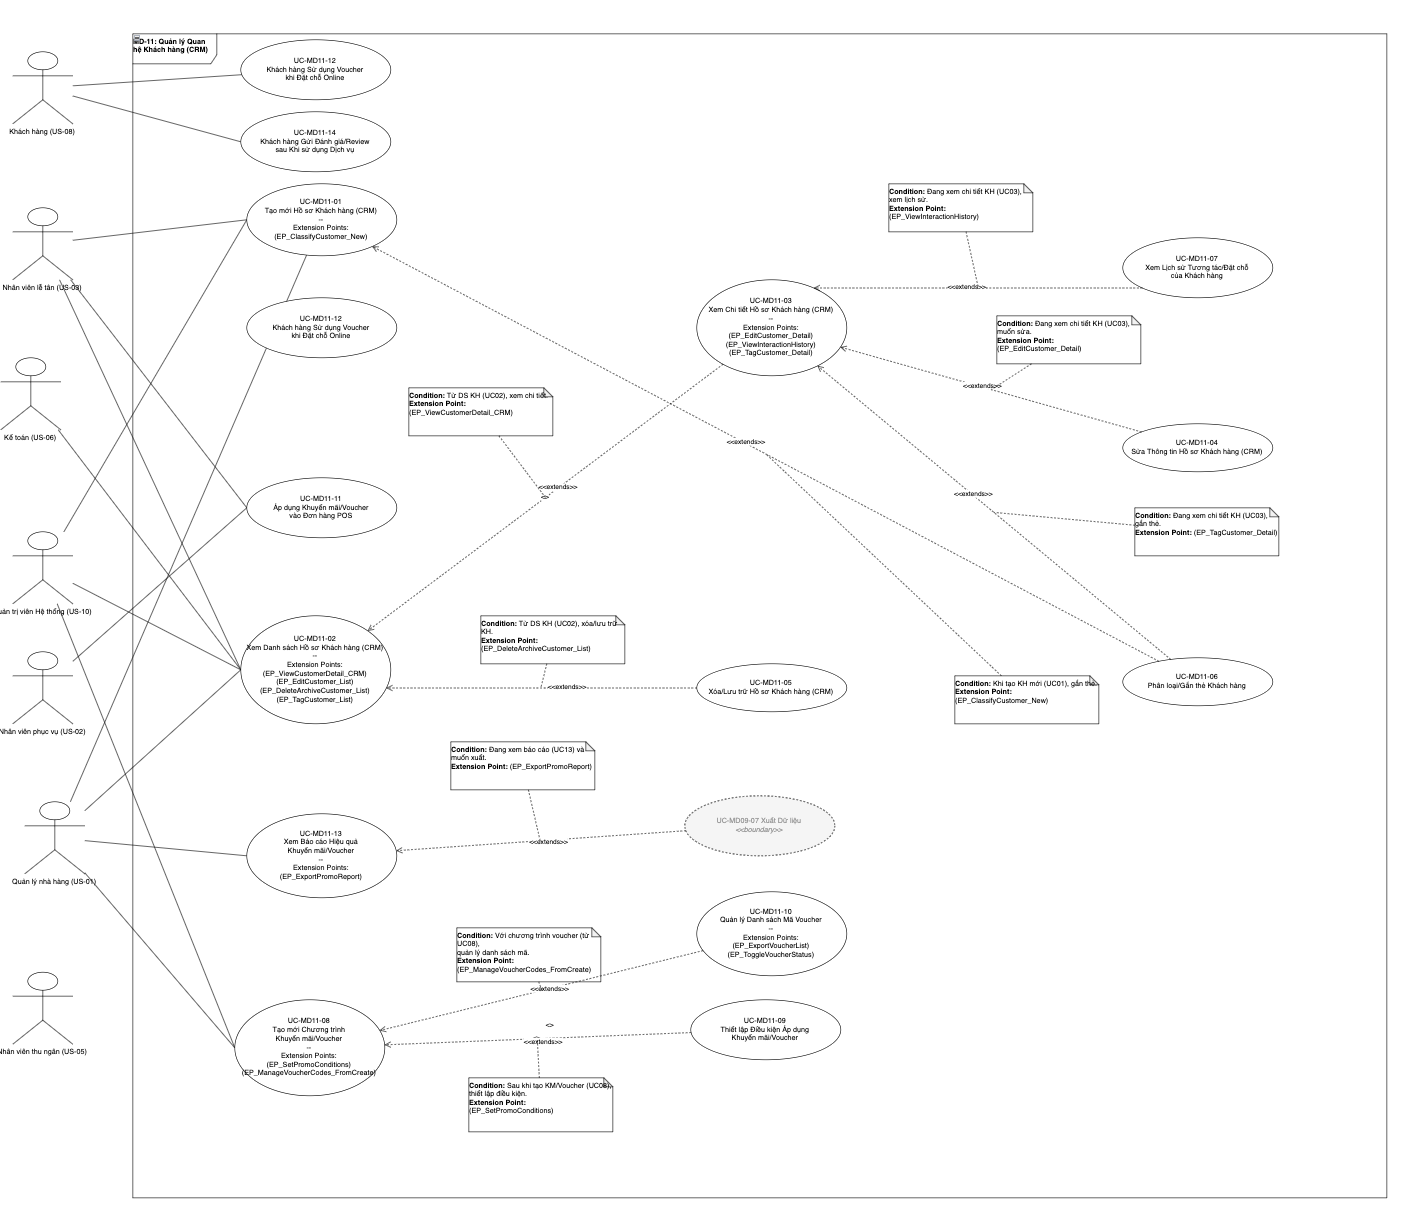
\includegraphics[width=15cm]{Sections/tong_quan/functional_spec/img/uc11.png}
    \vspace{0.5cm}
    \caption{Use case diagram cho Module MD-11}
    \label{fig:my_label}
\end{figure}

\begin{longtable}{|m{2cm}|m{2.5cm}|m{2.5cm}|m{4.5cm}|m{4cm}|}
\caption{Danh sách Yêu cầu Chức năng cho Module MD-11: Quản lý Quan hệ Khách hàng (CRM)} \label{tab:fr_md11_crm_marketing_revised_in_codeblock} \\
\hline
\textbf{Mã Module} & \textbf{Mã Yêu cầu CN} & \textbf{Mã Người dùng} & \textbf{Tên Chức năng} & \textbf{Mô tả Ngắn} \\
\hline
\endhead % Header cho các trang tiếp theo
\midrule
\endfoot % Footer cho bảng
\bottomrule
\endlastfoot % Footer cho trang cuối cùng

% === Quản lý Hồ sơ Khách hàng (CRM View) - Tách nhỏ ===
MD-11 & FR-MD11-01 & US-01, US-03, US-10 & Tạo mới Hồ sơ Khách hàng (CRM) & Nhân viên/Quản lý tạo hồ sơ mới cho khách hàng với các thông tin chi tiết. \\
\hline
MD-11 & FR-MD11-02 & US-01, US-03, US-10 & Xem Danh sách Hồ sơ Khách hàng (CRM) & Xem danh sách tất cả khách hàng trong hệ thống CRM, có thể tìm kiếm, lọc. \\
\hline
MD-11 & FR-MD11-03 & US-01, US-03, US-10 & Xem Chi tiết Hồ sơ Khách hàng (CRM) & Xem toàn bộ thông tin chi tiết của một khách hàng cụ thể (thông tin cá nhân, lịch sử, sở thích...). \\
\hline
MD-11 & FR-MD11-04 & US-01, US-03, US-10 & Sửa Thông tin Hồ sơ Khách hàng (CRM) & Cập nhật, chỉnh sửa các thông tin trong hồ sơ của một khách hàng đã có. \\
\hline
MD-11 & FR-MD11-05 & US-01, US-10 & Xóa/Lưu trữ Hồ sơ Khách hàng (CRM) & Xóa (nếu chưa có giao dịch) hoặc lưu trữ (ẩn đi) hồ sơ khách hàng không còn hoạt động. \\
\hline
MD-11 & FR-MD11-06 & US-01, US-06, US-10 & Phân loại/Gắn thẻ Khách hàng & Phân loại khách hàng (VIP, thường xuyên...) hoặc gắn thẻ (tag) cho khách hàng để phục vụ marketing, chăm sóc. \\
\hline
MD-11 & FR-MD11-07 & US-01, US-06, US-10 & Xem Lịch sử Tương tác/Đặt chỗ của Khách hàng & Truy cập toàn bộ lịch sử đặt chỗ, hóa đơn, phản hồi, ghi chú tương tác của một khách hàng cụ thể. \\
\hline

% === Quản lý Voucher/Khuyến mãi ===
MD-11 & FR-MD11-08 & US-01, US-10 & Tạo mới Chương trình Khuyến mãi/Voucher & Định nghĩa các chương trình khuyến mãi (giảm giá \%, giảm tiền cố định, mua X tặng Y) hoặc tạo mã voucher. \\
\hline
MD-11 & FR-MD11-09 & US-01, US-10 & Thiết lập Điều kiện Áp dụng Khuyến mãi/Voucher & Cấu hình điều kiện: thời gian, giá trị đơn tối thiểu, sản phẩm/danh mục áp dụng, số lần sử dụng... \\
\hline
MD-11 & FR-MD11-10 & US-01, US-10 & Quản lý Danh sách Mã Voucher & Xem danh sách mã voucher đã tạo, trạng thái (đã dùng, còn hạn), có thể xuất mã hàng loạt, vô hiệu hóa voucher. \\
\hline
MD-11 & FR-MD11-11 & US-02, US-05 & Áp dụng Khuyến mãi/Voucher vào Đơn hàng POS & Nhân viên POS nhập mã voucher hoặc chọn chương trình khuyến mãi đủ điều kiện để áp dụng cho đơn hàng. \\
\hline
MD-11 & FR-MD11-12 & US-08 & Khách hàng Sử dụng Voucher khi Đặt chỗ Online & Khách hàng nhập mã voucher hợp lệ vào đơn đặt chỗ/đặt món online để được giảm giá. \\
\hline
MD-11 & FR-MD11-13 & US-01 & Xem Báo cáo Hiệu quả Khuyến mãi/Voucher & Thống kê số lần sử dụng, tổng giá trị giảm giá của từng chương trình/voucher. (Mở rộng từ UC-MD09-09) \\
\hline

% === Thu thập & Quản lý Đánh giá/Phản hồi ===
MD-11 & FR-MD11-14 & US-08 & Khách hàng Gửi Đánh giá/Review sau Khi sử dụng Dịch vụ & Khách hàng (có thể qua email mời hoặc link trên hóa đơn) gửi đánh giá về chất lượng món ăn, dịch vụ. \\
\hline
MD-11 & FR-MD11-15 & US-01, US-09 & Xem và Quản lý Đánh giá/Phản hồi của Khách hàng & Quản lý xem các đánh giá, có thể phản hồi, phân loại (tích cực, tiêu cực), hoặc đánh dấu đã xử lý. \\
\hline
MD-11 & FR-MD11-16 & US-01 & (Tùy chọn) Hiển thị Đánh giá Tích cực trên Website & Chọn lọc và hiển thị các đánh giá tốt của khách hàng trên trang web nhà hàng (nếu muốn). \\
\hline
% Các chức năng khác như Loyalty, Email Marketing sẽ được thêm vào sau nếu cần
\end{longtable}

\subsubsubsection{Mục tiêu và Phạm vi}
\label{sssec:md11_objectives_scope}
Mục tiêu chính của module MD-11 là:
\begin{itemize}
    \item \textbf{Xây dựng cơ sở dữ liệu khách hàng toàn diện:} Lưu trữ thông tin liên hệ, lịch sử giao dịch, sở thích và các ghi chú quan trọng về từng khách hàng.
    \item \textbf{Phân loại và phân khúc khách hàng:} Cho phép gắn thẻ, phân loại khách hàng (ví dụ: VIP, khách thường xuyên) để phục vụ các chiến dịch chăm sóc và marketing cá nhân hóa.
    \item \textbf{Quản lý chương trình khuyến mãi và voucher hiệu quả:} Tạo, cấu hình điều kiện áp dụng, theo dõi việc sử dụng và đánh giá hiệu quả của các chương trình khuyến mãi và mã voucher.
    \item \textbf{Thu thập và quản lý phản hồi của khách hàng:} Cung cấp kênh cho khách hàng gửi đánh giá và cho phép nhà hàng xem xét, phân tích các phản hồi này.
    \item \textbf{Tăng cường tương tác và chăm sóc khách hàng:} Cung cấp thông tin để nhân viên có thể phục vụ khách hàng tốt hơn và xây dựng mối quan hệ lâu dài.
    \item \textbf{Hỗ trợ các hoạt động marketing:} Cung cấp dữ liệu khách hàng cho việc tạo các chiến dịch email marketing hoặc các hoạt động quảng bá khác (có thể tích hợp với module marketing riêng).
\end{itemize}
Phạm vi của module bao gồm việc quản lý hồ sơ khách hàng từ khi tạo mới, cập nhật thông tin, theo dõi lịch sử, cho đến việc thiết kế và quản lý các chương trình khuyến mãi/voucher, cũng như quy trình thu thập và xem xét đánh giá từ khách hàng.

\subsubsubsection{Đối tượng Sử dụng Chính}
\label{sssec:md11_primary_users}
Các đối tượng người dùng chính tương tác với module này bao gồm:
\begin{itemize}
    \item \textbf{US-01 (Quản lý nhà hàng):} Là người dùng chính, chịu trách nhiệm tạo và quản lý các chương trình khuyến mãi, xem báo cáo hiệu quả, quản lý hồ sơ khách hàng VIP, và xem xét các đánh giá của khách hàng.
    \item \textbf{US-03 (Nhân viên lễ tân):} Thường xuyên tạo mới và cập nhật hồ sơ khách hàng, có thể xem lịch sử đặt chỗ của khách để hỗ trợ tốt hơn.
    \item \textbf{US-06 (Kế toán):} Có thể cần xem thông tin khách hàng liên quan đến hóa đơn hoặc các chương trình khách hàng thân thiết.
    \item \textbf{US-10 (Quản trị viên Hệ thống):} Có thể tham gia vào việc cấu hình ban đầu của module CRM, tạo các trường tùy chỉnh hoặc thiết lập các quy tắc tự động (nếu có).
    \item \textbf{US-08 (Khách hàng):} Là người cung cấp thông tin cá nhân, sử dụng voucher khi đặt chỗ online, và gửi đánh giá/review về dịch vụ.
    \item \textbf{US-02 (Nhân viên phục vụ) / US-05 (Nhân viên thu ngân):} Áp dụng các chương trình khuyến mãi hoặc mã voucher cho đơn hàng tại POS.
\end{itemize}

\subsubsubsection{Các Chức năng Chính}
\label{sssec:md11_key_functionalities}
Module MD-11 cung cấp một bộ các chức năng tập trung vào việc quản lý và tăng cường mối quan hệ với khách hàng:

\begin{itemize}
    \item \textbf{Quản lý Hồ sơ Khách hàng (UC-MD11-01 đến UC-MD11-07):}
    \begin{itemize}
        \item Tạo mới một hồ sơ khách hàng trong hệ thống CRM với các thông tin liên hệ cơ bản (UC-MD11-01).
        \item Xem danh sách tất cả các hồ sơ khách hàng với khả năng tìm kiếm và lọc (UC-MD11-02).
        \item Xem thông tin chi tiết đầy đủ của một hồ sơ khách hàng, bao gồm lịch sử giao dịch và tương tác (UC-MD11-03).
        \item Sửa đổi và cập nhật các thông tin trong một hồ sơ khách hàng đã tồn tại (UC-MD11-04).
        \item Xóa vĩnh viễn (nếu không có giao dịch) hoặc lưu trữ (ẩn đi) các hồ sơ khách hàng không còn phù hợp (UC-MD11-05).
        \item Gán các thẻ (tags) hoặc phân loại khách hàng (ví dụ: VIP, Thường xuyên) để phục vụ việc nhóm và phân tích (UC-MD11-06).
        \item Truy cập và xem lại toàn bộ lịch sử các hoạt động và giao dịch liên quan đến một khách hàng cụ thể (UC-MD11-07).
    \end{itemize}

    \item \textbf{Quản lý Chương trình Khuyến mãi và Voucher (UC-MD11-08 đến UC-MD11-13):}
    \begin{itemize}
        \item Định nghĩa một chương trình khuyến mãi mới hoặc một lô mã voucher mới, bao gồm loại hình và giá trị khuyến mãi (UC-MD11-08).
        \item Thiết lập các điều kiện và quy tắc chi tiết để chương trình/voucher có thể được áp dụng (ví dụ: thời gian hiệu lực, giá trị đơn hàng tối thiểu, sản phẩm áp dụng) (UC-MD11-09).
        \item Xem danh sách các mã voucher đã tạo, kiểm tra trạng thái, và có thể thực hiện xuất file hoặc vô hiệu hóa mã (UC-MD11-10).
        \item Nhân viên tại POS áp dụng một chương trình khuyến mãi hoặc nhập mã voucher hợp lệ vào đơn hàng của khách (UC-MD11-11).
        \item Khách hàng tự nhập và sử dụng mã voucher hợp lệ khi thực hiện đặt chỗ hoặc đặt món trước trực tuyến (UC-MD11-12).
        \item Xem báo cáo thống kê chi tiết về tình hình sử dụng và hiệu quả của các chương trình khuyến mãi hoặc voucher (UC-MD11-13).
    \end{itemize}

    \item \textbf{Quản lý Đánh giá và Phản hồi từ Khách hàng (UC-MD11-14, và sẽ có các UC tiếp theo như UC-MD11-15, UC-MD11-16):}
    \begin{itemize}
        \item Cho phép khách hàng gửi các ý kiến đánh giá, nhận xét, hoặc xếp hạng về dịch vụ của nhà hàng thông qua các kênh trực tuyến (UC-MD11-14).
        \item (Dự kiến) Cho phép Quản lý nhà hàng xem danh sách các đánh giá đã nhận được.
        \item (Dự kiến) Cho phép Quản lý nhà hàng xem chi tiết một đánh giá cụ thể và có thể thực hiện các hành động phản hồi.
    \end{itemize}
\end{itemize}

\subsubsubsection{Tóm tắt Luồng Hoạt động Tổng thể}
\label{sssec:md11_overall_workflow}
Luồng hoạt động trong module Quản lý Quan hệ Khách hàng (CRM) thường bao gồm các giai đoạn và quy trình sau:
\begin{enumerate}
    \item \textbf{Thu thập và Quản lý Thông tin Khách hàng:}
        \begin{itemize}
            \item Nhân viên Tạo mới Hồ sơ Khách hàng (CRM) (UC-MD11-01) khi có khách mới hoặc nhập dữ liệu.
            \item Nhân viên thường xuyên Xem Danh sách Hồ sơ Khách hàng (UC-MD11-02), Xem Chi tiết Hồ sơ Khách hàng (UC-MD11-03) để tra cứu, và Sửa Thông tin Hồ sơ Khách hàng (UC-MD11-04) khi cần cập nhật.
            \item Thực hiện Phân loại/Gắn thẻ Khách hàng (UC-MD11-06) để phục vụ các mục đích khác nhau.
            \item Khi cần, Xóa/Lưu trữ Hồ sơ Khách hàng (CRM) (UC-MD11-05).
            \item Xem Lịch sử Tương tác/Đặt chỗ của Khách hàng (UC-MD11-07) để hiểu rõ hơn về khách.
        \end{itemize}
    \item \textbf{Triển khai và Quản lý Chương trình Khuyến mãi/Voucher:}
        \begin{itemize}
            \item Quản lý Tạo mới Chương trình Khuyến mãi/Voucher (UC-MD11-08).
            \item Thiết lập Điều kiện Áp dụng Khuyến mãi/Voucher (UC-MD11-09) chi tiết cho từng chương trình.
            \item (Nếu là voucher) Quản lý Danh sách Mã Voucher (UC-MD11-10), có thể xuất file hoặc vô hiệu hóa mã.
            \item Nhân viên tại POS Áp dụng Khuyến mãi/Voucher vào Đơn hàng POS (UC-MD11-11) cho khách.
            \item Khách hàng Sử dụng Voucher khi Đặt chỗ Online (UC-MD11-12) trên website/app.
            \item Quản lý định kỳ Xem Báo cáo Hiệu quả Khuyến mãi/Voucher (UC-MD11-13) để đánh giá.
        \end{itemize}
    \item \textbf{Thu thập và Xử lý Phản hồi Khách hàng:}
        \begin{itemize}
            \item Khách hàng Gửi Đánh giá/Review sau Khi sử dụng Dịch vụ (UC-MD11-14).
            \item (Dự kiến) Quản lý xem xét các đánh giá này và có thể phản hồi hoặc thực hiện các hành động cải thiện dịch vụ.
        \end{itemize}
\end{enumerate}
Module MD-11 giúp nhà hàng không chỉ quản lý giao dịch mà còn xây dựng mối quan hệ ý nghĩa với khách hàng, từ đó tạo lợi thế cạnh tranh và phát triển bền vững.




% \subsection{Yêu cầu chất lương}

% % \subsubsection{Yêu cầu chức năng}

% Trong phạm vi đồ án này, chúng em sẽ tập trung vào các đối tượng chính sử dụng hệ thống, bao gồm Khách hàng, Nhân viên phục vụ, Nhân viên thu ngân, Nhân viên chăm sóc khách hàng, Nhân viên bếp, Quản lý chi nhánh và Quản lý tổng, nhằm đảm bảo hệ thống đáp ứng tốt nhu cầu vận hành và trải nghiệm của từng vai trò.

% \begin{figure}[H]
%     \centering
%     \includegraphics[width=15cm]{Images/nguoi-dung-he-thong.png}
%     \vspace{0.5cm}
%     \caption{Các đối tượng người dùng của hệ thống}
%     \label{fig:my_label}
% \end{figure}

% \textbf{Đối với Khách hàng}
% \begin{itemize}
%     \item Đăng ký, đăng nhập
%     \item Gửi yêu cầu đặt bàn trực tuyến, xem được tổng quan vị trí, trạng thái bàn thông qua các sơ đồ
%     \item Hủy yêu cầu đặt bàn cho đến khi trước thời gian hẹn 2 tiếng
%     \item Quét QR để truy cập vào menu và đặt món, không cần gọi nhân viên
%     \item Xem danh sách món ăn và đồ uống, kèm theo hình ảnh, mô tả và giá cả
%     \item Tìm kiếm món ăn theo tên hoặc danh mục, giá cả
%     \item Chọn món, số lượng và tùy chọn (size, topping, gia vị)
%     \item Gợi ý món ăn phù hợp dựa trên lịch sử đơn hàng và số liệu phân tích
%     \item Thêm món vào giỏ hàng
%     \item Xem lại giỏ hàng trước khi xác nhận đặt món
%     \item Đặt món nhiều lần trong cùng một lượt sử dụng tại nhà hàng, để có thể thay đổi món ăn trong suốt quá trình ăn
%     \item Gửi yêu cầu hủy đơn hoặc hủy/thay đổi các món cụ thể
%     \item Xem lại các đơn hàng đã đặt trước đó
%     \item Xem chi tiết các món đã đặt, tổng tiền và các khuyến mãi (nếu có)
%     \item Gửi yêu cầu thanh toán bằng cách quét mã QR, hoặc thao tác trên ứng dụng
%     \item Nhận thông báo về các khuyến mãi và ưu đãi
%     \item Gửi phản hồi về món ăn hoặc dịch vụ
%     \item Gửi khiếu nại nếu có sự cố
%     \item Trò chuyện trực tiếp với nhân viên chăm sóc khách hàng
% \end{itemize}

% \textbf{Đối với Phục vụ}
% \begin{itemize}
%     \item Xem danh sách trạng thái bàn
%     \item Hỗ trợ khách hàng đặt món, thanh toán
%     \item Xem danh sách đơn hàng của khách
%     \item Nhận thông báo khi món ăn đã sẵn sàng
%     \item Xử lý yêu cầu hủy đơn hoặc hủy/thay đổi món của khách
%     \item Chuyển vị trí đơn hàng sang bàn khác.
%     \item Đặt lại trạng thái bàn
% \end{itemize}

% \textbf{Đối với Thu ngân}
% \begin{itemize}
%     \item Nhận thông báo khi có yêu cầu thanh toán
%     \item Xem chi tiết đơn hàng và tổng hóa đơn
%     \item Áp dụng khuyến mãi và giảm giá khi thanh toán
%     \item Quản lý các phương thức thanh toán
%     \item Nhận thông báo về thanh toán thành công với phương thức quét QR, quẹt thẻ
%     \item Cập nhật trạng thái thanh toán với phương thức thanh toán tiền mặt
%     \item In hóa đơn cho khách hàng
%     \item Xử lý yêu cầu hoàn tiền (vấn đề phát sinh)
%     \item Tạo báo cáo doanh thu hàng ngày
% \end{itemize}

% \textbf{Đối với Nhân viên chăm sóc khách hàng}
% \begin{itemize}
%     \item Tiếp nhận và xử lý yêu cầu từ khách hàng
%     \item Theo dõi và quản lý khiếu nại \& phản hồi từ khách hàng
%     \item Trả lời tin nhắn trực tuyến với khách hàng
%     \item Cập nhật thông tin khách hàng
%     \item Theo dõi và nhắc nhở khách hàng về các chương trình ưu đãi qua tài khoản và email
% \end{itemize}

% \textbf{Đối với Nhân viên bếp}
% \begin{itemize}
%     \item Nhận đơn hàng từ hệ thống quản lý đơn hàng
%     \item Xem tất cả danh sách món ăn được sắp xếp theo thứ tự ưu tiên
%     \item Xem được các yêu cầu đặc biệt của từng món ăn cần làm
%     \item Cập nhật trạng thái chế biến của từng món ăn (chưa làm, đang chế biến, hoàn thành...)
% \end{itemize}

% \textbf{Đối với Quản lý chi nhánh}
% \begin{itemize}
%     \item Thêm/Chỉnh sửa sơ đồ nhà hàng
%     \item Xử lý, xác nhận các yêu cầu đặt bàn của khách hàng tại chi nhánh
%     \item Xem báo cáo kinh doanh và doanh thu của chi nhánh
%     \item Điều chỉnh và thiết lập các chương trình khuyến mãi, marketing chi nhánh
%     \item Theo dõi các phản hồi của khách hàng
%     \item Xem danh sách nhân viên
%     \item Phân chia công việc cho các tài khoản nhân viên
% \end{itemize}

% \textbf{Đối với Quản lý tổng}
% \begin{itemize}
%     \item Quản lý thông tin chi nhánh
%     \item Thêm/Xóa chi nhánh
%     \item Quản lý các tài khoản nhân viên và khách hàng
%     \item Xem báo cáo tổng quan tất cả các chi nhánh
%     \item Xem báo cáo chi tiết của một chi nhánh tổng
% \end{itemize}

% % User Story là một kỹ thuật phát triển phần mềm tập trung vào nhu cầu của người dùng trong quá trình sử dụng sản phẩm. Mục đích của User Story là giúp các nhà phát triển phần mềm hiểu rõ những tính năng cốt lõi của sản phẩm và xác định được các chức năng cần thiết để hiện thực đầu tiên của ứng dụng.\\

% % Để đưa ra danh sách User Story của ứng dụng, nhóm chúng em đã tiến hành thảo luận, nghiên cứu và phân tích yêu cầu của người dùng. Chúng tôi bắt đầu xây dựng hệ thống tuyển dụng bằng cách xác định các tính năng cơ bản cần phải có trong ứng dụng để đáp ứng nhu cầu và mong muốn của người dùng.\\

% % \textbf{Một số user story cơ bản như sau:}
% % \begin{itemize}
% %     \item Đối với Khách hàng
% %     \begin{enumerate}
% %         \item Là Khách Hàng, tôi muốn quét mã QR trên bàn để truy cập vào menu và đặt món.
% %         \item Là Khách Hàng, tôi muốn xem danh sách các món ăn và đồ uống, kèm theo hình ảnh, mô tả và giá cả.
% %         \item Là Khách Hàng, tôi muốn tìm kiếm món ăn theo tên hoặc danh mục.
% %         \item Là Khách Hàng, tôi muốn chọn món, số lượng và các tùy chọn (ví dụ: size, topping, gia vị).
% %         \item Là Khách Hàng, tôi muốn thêm các món đã chọn vào giỏ hàng.
% %         \item Là Khách Hàng, tôi muốn xem lại giỏ hàng trước khi xác nhận đặt món.
% %         \item Là Khách Hàng, tôi muốn đặt món nhiều lần trong cùng một lượt sử dụng tại nhà hàng.
% %         \item Là Khách Hàng, tôi muốn xem lại các order đã đặt trước đó (nếu đã đăng nhập).
% %         \item Là Khách Hàng, tôi muốn xem chi tiết các món đã đặt, tổng tiền và các khuyến mãi (nếu có).
% %         \item Là Khách Hàng, tôi muốn thanh toán bằng cách quét mã QR hoặc thanh toán tiền mặt.
% %         \item Là Khách Hàng, tôi muốn xem lại hóa đơn sau khi đã thanh toán.
% %         \item Là Khách Hàng, tôi muốn đăng ký tài khoản thành viên để tham gia chương trình khách hàng thân thiết.
% %         \item Là Khách Hàng, tôi muốn đăng nhập để xem lịch sử đặt món, nhận khuyến mãi và các ưu đãi khác.
% %     \end{enumerate}
% %     \item Đối với Nhân Viên Thu Ngân/Phục Vụ
% %     \begin{enumerate}
% %         \item Là Nhân Viên Thu Ngân/Phục Vụ, tôi muốn xem danh sách các order mới và đang chờ xử lý.
% %         \item Là Nhân Viên Thu Ngân/Phục Vụ, tôi muốn xem chi tiết các order của khách hàng.
% %         \item Là Nhân Viên Thu Ngân/Phục Vụ, tôi muốn gộp các order của một bàn thành một hóa đơn duy nhất.
% %         \item Là Nhân Viên Thu Ngân/Phục Vụ, tôi muốn xóa bỏ các order nếu cần.
% %         \item Là Nhân Viên Thu Ngân/Phục Vụ, tôi muốn xác nhận thanh toán bằng QR.
% %         \item Là Nhân Viên Thu Ngân/Phục Vụ, tôi muốn xác nhận thanh toán bằng tiền mặt (tự thao tác).
% %         \item Là Nhân Viên Thu Ngân/Phục Vụ, tôi muốn in hóa đơn cho khách hàng (có mã QR để thanh toán).
% %         \item Là Nhân Viên Thu Ngân/Phục Vụ, tôi muốn check-in (chấm công) đầu ca và check-out (chấm công) cuối ca.
% %         \item Là Nhân Viên Thu Ngân/Phục Vụ, tôi muốn chuyển order từ bàn này sang bàn khác (nếu khách hàng muốn đổi bàn).
% %     \end{enumerate}
% %     \item Đối với Quản Lý Chi Nhánh
% %     \begin{enumerate}
% %         \item Là Quản Lý Chi Nhánh, tôi muốn nhập kho, xem danh sách các nguyên liệu trong kho.
% %         \item Là Quản Lý Chi Nhánh, tôi muốn theo dõi số lượng còn lại của từng nguyên liệu.
% %         \item Là Quản Lý Chi Nhánh, tôi muốn xem báo cáo nhập/xuất kho hàng ngày.
% %         \item Là Quản Lý Chi Nhánh, tôi muốn xem danh sách nhân viên.
% %         \item Là Quản Lý Chi Nhánh, tôi muốn phân công ca làm cho nhân viên.
% %         \item Là Quản Lý Chi Nhánh, tôi muốn xem lịch sử check-in/check-out của nhân viên.
% %         \item Là Quản Lý Chi Nhánh, tôi muốn xem các báo cáo về doanh thu và số lượng món ăn bán được trong chi nhánh.
% %         \item Là Quản Lý Chi Nhánh, tôi muốn xem các báo cáo về kho nguyên liệu.
% %         \item Là Quản Lý Chi Nhánh, tôi muốn xem danh sách bàn đang có.
% %         \item Là Quản Lý Chi Nhánh, tôi muốn sắp xếp bàn cho khách hàng và quản lý bàn trống.
% %     \end{enumerate}
% %     \item Đối với Quản Lý Tổng
% %     \begin{enumerate}
% %         \item Là Quản Lý Tổng, tôi muốn xem tổng doanh thu của tất cả các chi nhánh.
% %         \item Là Quản Lý Tổng, tôi muốn xem chi tiết doanh thu của từng chi nhánh, theo ngày, tuần, tháng, năm.
% %         \item Là Quản Lý Tổng, tôi muốn xem các báo cáo tổng quan về hoạt động của nhà hàng.
% %         \item Là Quản Lý Tổng, tôi muốn xuất báo cáo tổng quan về doanh thu, chi phí và lợi nhuận.
% %         \item Là Quản Lý Tổng, tôi muốn xem danh sách tất cả các chi nhánh.
% %         \item Là Quản Lý Tổng, tôi muốn thêm, sửa hoặc xóa thông tin chi nhánh.
% %         \item Là Quản Lý Tổng, tôi muốn xem các báo cáo tổng quan từ các chi nhánh.
% %         \item Là Quản Lý Tổng, tôi muốn thêm, chỉnh sửa hoặc xóa các món ăn và đồ uống trong thực đơn.
% %         \item Là Quản Lý Tổng, tôi muốn thay đổi giá cả, mô tả và hình ảnh của món ăn.
% %     \end{enumerate}
% %     \item Các Tính Năng Mở Rộng (Optional)
% %     \begin{enumerate}
% %         \item Là Khách Hàng, tôi muốn hệ thống gợi ý món ăn dựa trên lịch sử đặt món của mình.
% %         \item Là Quản Lý (Tổng/Chi Nhánh), tôi muốn tạo và quản lý các chương trình khuyến mãi, giảm giá.
% %         \item Là Khách Hàng, tôi muốn đặt bàn trước thông qua ứng dụng.
% %         \item Là Khách Hàng, tôi muốn đánh giá chất lượng món ăn và dịch vụ của nhà hàng.
% %         \item Là Quản Lý (Tổng/Chi Nhánh), tôi muốn hệ thống tự động xuất dữ liệu sang hệ thống kế toán.
% %     \end{enumerate}
% % \end{itemize}

% % \textbf{Một số usecase diagram cơ bản như sau:}

% % \begin{figure}[H]
% %     \centering
% %     \includegraphics[width=15cm]{Images/us-dat-mon.png}
% %     \vspace{0.5cm}
% %     \caption{Các use case liên quan đến đặt món}
% %     \label{fig:my_label}
% % \end{figure}

% % \begin{figure}[H]
% %     \centering
% %     \includegraphics[width=15cm]{Images/us-tai-khoan.png}
% %     \vspace{0.5cm}
% %     \caption{Các use case liên quan đến quản lý tài khoản}
% %     \label{fig:my_label}
% % \end{figure}

% % \begin{figure}[H]
% %     \centering
% %     \includegraphics[width=15cm]{Images/us-quan-ly.png}
% %     \vspace{0.5cm}
% %     \caption{Các use case liên quan đến quản lý}
% %     \label{fig:my_label}
% % \end{figure}

% % \begin{enumerate}[(a)]
% %     \item Khách hàng
% %     \begin{itemize}
% %         \item Quét mã QR
% %         \begin{itemize}
% %             \item Khách hàng quét mã QR trên bàn để truy cập vào menu và đặt món.
% %         \end{itemize}
% %         \item Xem menu
% %         \begin{itemize}
% %             \item Xem danh sách các món ăn và đồ uống, kèm theo hình ảnh, mô tả, giá cả.
% %             \item Tìm kiếm món ăn theo tên hoặc danh mục.
% %         \end{itemize}
% %         \item Đặt món
% %         \begin{itemize}
% %             \item Chọn món, số lượng, tùy chọn (ví dụ: size, topping, gia vị)
% %             \item Thêm món vào giỏ hàng.
% %             \item Xem lại giỏ hàng trước khi xác nhận đặt món.
% %             \item Đặt món nhiều lần trong cùng một lượt sử dụng.
% %         \end{itemize}
% %         \item Xem lịch sử đặt món
% %         \begin{itemize}
% %             \item Xem lại các order đã đặt trước đó (nếu đã đăng nhập).
% %         \end{itemize}
% %         \item Xem hóa đơn
% %         \begin{itemize}
% %             \item Xem chi tiết các món đã đặt, tổng tiền, các khuyến mãi (nếu có).
% %         \end{itemize}
% %         \item Thanh toán
% %         \begin{itemize}
% %             \item Thanh toán bằng cách quét mã QR hoặc thanh toán tiền mặt.
% %             \item Xem lại hóa đơn sau khi đã thanh toán.
% %         \end{itemize}
% %         \item Đăng ký/Đăng nhập (Tùy chọn)
% %         \begin{itemize}
% %             \item Đăng ký tài khoản thành viên để tham gia chương trình khách hàng thân thiết.
% %             \item Đăng nhập để xem lịch sử đặt món, nhận khuyến mãi và các ưu đãi khác.
% %         \end{itemize}
% %     \end{itemize}
% %     \item Nhân viên thu ngân/phục vụ
% %     \begin{itemize}
% %         \item Quản lý order
% %         \begin{itemize}
% %             \item Xem danh sách các order mới và đang chờ xử lý.
% %             \item Xem chi tiết các order của khách hàng.
% %         \end{itemize}
% %         \item Gộp hóa đơn
% %         \begin{itemize}
% %             \item Gộp các order của một bàn thành một hóa đơn duy nhất.
% %             \item Xóa bỏ các order (nếu cần)
% %         \end{itemize}
% %         \item Xác nhận thanh toán
% %         \begin{itemize}
% %             \item Xác nhận thanh toán bằng QR.
% %             \item Xác nhận thanh toán bằng tiền mặt (tự thao tác).
% %         \end{itemize}
% %         \item In hóa đơn
% %         \begin{itemize}
% %             \item In hóa đơn cho khách hàng (có mã QR để thanh toán).
% %         \end{itemize}
% %         \item Check-in/Check-out
% %         \begin{itemize}
% %             \item Chấm công đầu ca và cuối ca.
% %         \end{itemize}
% %         \item Chuyển Order
% %         \begin{itemize}
% %             \item Có thể chuyển order từ bàn này sang bàn khác (nếu khách hàng muốn đổi bàn)
% %         \end{itemize}
% %     \end{itemize}
% %     \item Chức năng cho quản lý chi nhánh
% %     \begin{itemize}
% %         \item Quản lý kho nguyên liệu
% %         \begin{itemize}
% %             \item Nhập kho, xem danh sách các nguyên liệu trong kho.
% %             \item Theo dõi số lượng còn lại của từng nguyên liệu.
% %             \item Báo cáo nhập/xuất kho hàng ngày.
% %         \end{itemize}
% %         \item Quản lý nhân viên
% %         \begin{itemize}
% %             \item Xem danh sách nhân viên.
% %             \item Phân công ca làm.
% %             \item Xem lịch sử check-in/check-out của nhân viên.
% %         \end{itemize}
% %         \item Xem báo cáo
% %         \begin{itemize}
% %             \item Xem các báo cáo về doanh thu, số lượng món ăn bán được trong chi nhánh.
% %             \item Xem các báo cáo về kho nguyên liệu.
% %         \end{itemize}
% %         \item Quản lý bàn
% %         \begin{itemize}
% %             \item Xem danh sách bàn đang có.
% %             \item Có thể sắp xếp bàn cho khách hàng, quản lý bàn trống.
% %         \end{itemize}
% %     \end{itemize}
% %     \item Chức năng cho quản lý tổng
% %     \begin{itemize}
% %         \item Quản lý doanh thu
% %         \begin{itemize}
% %             \item Xem tổng doanh thu của tất cả các chi nhánh.
% %             \item Xem chi tiết doanh thu của từng chi nhánh, theo ngày, tuần, tháng, năm.
% %         \end{itemize}
% %         \item Xem báo cáo
% %         \begin{itemize}
% %             \item Xem các báo cáo tổng quan về hoạt động của nhà hàng.
% %             \item Xuất báo cáo tổng quan về doanh thu, chi phí, lợi nhuận.
% %         \end{itemize}
% %         \item Quản lý chi nhánh
% %         \begin{itemize}
% %             \item Xem danh sách tất cả các chi nhánh.
% %             \item Thêm/sửa/xóa thông tin chi nhánh.
% %             \item Xem các báo cáo tổng quan từ các chi nhánh.
% %         \end{itemize}
% %         \item Quản lý thực đơn
% %         \begin{itemize}
% %             \item Thêm, chỉnh sửa, xóa các món ăn và đồ uống trong thực đơn.
% %             \item Thay đổi giá cả, mô tả, hình ảnh của món ăn.
% %         \end{itemize}
% %     \end{itemize}
% %     \item Mở rộng (có thể làm nếu kịp thời gian)
% %     \begin{itemize}
% %         \item Hệ thống gợi ý món ăn: Dựa trên lịch sử đặt món của khách hàng, hệ thống có thể gợi ý các món ăn phù hợp.
% %         \item Hệ thống quản lý khuyến mãi: Cho phép tạo và quản lý các chương trình khuyến mãi, giảm giá.
% %         \item Hệ thống đặt bàn: Cho phép khách hàng đặt bàn trước thông qua ứng dụng.
% %         \item Hệ thống quản lý đánh giá: Cho phép khách hàng đánh giá chất lượng món ăn và dịch vụ của nhà hàng.
% %         \item Tích hợp với hệ thống kế toán: Tự động xuất dữ liệu sang hệ thống kế toán.
% %     \end{itemize}
% % \end{enumerate}

% \subsubsection{Yêu cầu phi chức năng}
% \begin{itemize}
%     \item Bảo mật:
%     \begin{itemize}
%         \item Dữ liệu người dùng và dữ liệu giao dịch phải được bảo vệ.
%         \item Hệ thống sử dụng HTTPS để đảm bảo an toàn cho quá trình truyền dữ liệu.
%     \end{itemize}

%     \item Hiệu năng:
%     \begin{itemize}
%         \item Hệ thống phải có tốc độ xử lý nhanh và ổn định.
%         \item Khả năng đáp ứng nhanh chóng khi nhiều người dùng truy cập cùng một lúc.    
%     \end{itemize}

%     \item Tính khả dụng:
%     \begin{itemize}
%         \item Hệ thống hoạt động ổn định và có thời gian uptime cao.
%         \item Giao diện thân thiện và dễ sử dụng trên cả web và mobile.
%     \end{itemize}

%     \item Khả năng mở rộng:
%     \begin{itemize}
%         \item Hệ thống có thể mở rộng để hỗ trợ thêm nhiều chi nhánh và người dùng.
%         \item Dễ dàng thêm các tính năng mới khi cần thiết.
%     \end{itemize}

% \end{itemize}












% \newpage
\section{THIẾT KẾ}
\subsection{Công nghệ sử dụng}
\subsubsection{Công nghệ Front-end}

\subsubsubsection{ReactJS}
    \begin{enumerate}[(a)]
        \item \textit{Giới thiệu}
        
            ReactJS là một thư viện JavaScript mã nguồn mở, được phát triển bởi Facebook, nhằm hỗ trợ xây dựng giao diện người dùng (UI) cho các ứng dụng web. Ra mắt vào năm 2013, ReactJS nhanh chóng trở thành một trong những công cụ phổ biến nhất cho việc phát triển UI tương tác và hiệu quả.
            
            % Các đặc điểm nổi bật của ReactJS:
    
            % \begin{itemize}
            %     \item \textbf{Kiến trúc dựa trên thành phần (Component-Based Architecture)}: React cho phép chia UI thành các thành phần nhỏ, độc lập và có thể tái sử dụng. Mỗi thành phần quản lý trạng thái và logic riêng, giúp việc phát triển và bảo trì ứng dụng trở nên dễ dàng hơn.
            %     \item \textbf{Virtual DOM}: React sử dụng một bản sao ảo của DOM thật, gọi là Virtual DOM. Khi có sự thay đổi trong trạng thái hoặc dữ liệu, React cập nhật Virtual DOM trước, sau đó so sánh với DOM thật và chỉ thực hiện những thay đổi cần thiết. Điều này cải thiện hiệu suất và tăng tốc độ render của ứng dụng.
            %     \item \textbf{JSX (JavaScript XML)}: React sử dụng JSX, một cú pháp mở rộng cho phép viết mã HTML trong JavaScript. Điều này giúp code trở nên dễ đọc và dễ hiểu hơn, đồng thời tối ưu hóa quá trình phát triển UI.
            %     \item \textbf{One-way Data Binding}: React áp dụng cơ chế liên kết dữ liệu một chiều, giúp luồng dữ liệu trở nên rõ ràng và dễ kiểm soát. Dữ liệu được truyền từ component cha đến component con thông qua props, giúp việc quản lý và debug ứng dụng trở nên hiệu quả hơn. 
            % \end{itemize}

        
        \item \textit{Ưu điểm} \cite{React}.

        \begin{itemize}
            \item  \textbf{Khai báo giao diện (Declarative)}: React giúp tạo ra các giao diện người dùng tương tác một cách dễ dàng. Bằng cách thiết kế các khung nhìn cho từng trạng thái trong ứng dụng, React sẽ tự động cập nhật và render các thành phần phù hợp khi dữ liệu thay đổi. Việc khai báo giao diện một cách tường minh giúp mã nguồn dễ hiểu và dễ dàng gỡ lỗi hơn.
            \item \textbf{Component-Based}: React cho phép xây dựng các thành phần độc lập và quản lý trạng thái riêng biệt của chúng. Những thành phần này có thể được kết hợp để tạo ra các giao diện phức tạp. Việc viết logic của thành phần bằng JavaScript thay vì template giúp dễ dàng truyền dữ liệu và tránh thao tác trực tiếp với DOM.
            \item \textbf{Học một lần, viết ở mọi nơi (Learn Once, Write Anywhere)}: React không phụ thuộc vào kỹ năng công nghệ cụ thể, cho phép phát triển các tính năng mới mà không cần viết lại mã hiện có. React có thể render trên máy chủ bằng Node.js và xây dựng ứng dụng di động thông qua React Native 
        \end{itemize}

        \item \textit{So sánh React và các công nghệ khác} 
        
            Khi so sánh giữa các công nghệ phổ biến hiện nay như ReactJS, Angular, Vue.js và Svelte, chúng ta có thể thấy những đặc điểm riêng biệt của từng công nghệ, giúp lựa chọn được công nghệ phù hợp với nhu cầu và yêu cầu của dự án. Dựa theo tài liệu \cite{FrontCompare1} và \cite{FrontCompare2}, dưới đây là bảng so sánh chi tiết giữa ReactJS và các công nghệ khác:

            % \begin{longtable}{|p{3.5cm}|p{5.5cm}|p{5.5cm}|}
            % \hline
            % \textbf{Tiêu Chí} & \textbf{ReactJS} & \textbf{Angular} \\ 
            % \hline
            % \endfirsthead
            % \hline
            % \textbf{Tiêu Chí} & \textbf{ReactJS} & \textbf{Angular} \\ 
            % \endhead
            % \hline
            % % \multicolumn{3}{|r|}{\small\slshape Còn tiếp} \\ \hline
            % \endfoot
            % \hline
            % \endlastfoot
            % Ngôn ngữ & JavaScript (hỗ trợ TypeScript)     & TypeScript (bắt buộc)\\ 
            % \hline
            % Định nghĩa & Thư viện JavaScript để xây dựng giao diện người dùng & Framework toàn diện để phát triển ứng dụng web\\ 
            % \hline
            % Kiến trúc & Dựa trên thành phần, Virtual DOM, luồng dữ liệu một chiều & Dựa trên thành phần, MVC/MVVM, cơ chế phát hiện thay đổi\\ 
            % \hline
            % Thời gian phát triển & Nhanh cho dự án nhỏ, chậm hơn nếu cần tích hợp nhiều thư viện & Chậm hơn do cấu hình ban đầu phức tạp, nhanh cho dự án lớn nhờ tích hợp sẵn\\ 
            % \hline
            % Độ phức tạp & Trung bình, phụ thuộc vào cách quản lý trạng thái & Cao, nhiều khái niệm (Dependency Injection, RxJS, Modules)\\ 
            % \hline
            % Tính linh hoạt & Cao, tự do chọn thư viện và công cụ & Thấp hơn, bị ràng buộc bởi cấu trúc framework\\ 
            % \hline
            % Bảo trì & Dễ bảo trì với các thành phần nhỏ & Dễ bảo trì cho dự án lớn, khó hơn với dự án nhỏ do cấu trúc phức tạp\\ 
            % \hline
            % Dễ sử dụng/Dễ học & Dễ học với người biết JavaScript & Khó học, cần hiểu TypeScript và các khái niệm framework\\ 
            % \hline
            % Hỗ trợ cộng đồng & Rất lớn, nhiều tài liệu, thư viện và diễn đàn & Lớn, hỗ trợ chính thức từ Google, tài liệu chi tiết\\ 
            % \hline
            % Kiểm thử & Jest, React Testing Library, dễ thiết lập & Jasmine, Karma, tích hợp sẵn nhưng phức tạp hơn\\ 
            % \hline
            % \caption{Bảng so sánh ReactJS và Angular}\\
            % \end{longtable}

            % \begin{longtable}{|p{3.5cm}|p{5.5cm}|p{5.5cm}|}
            % \hline
            % \textbf{Tiêu Chí} & \textbf{Svelt} & \textbf{Vue.js} \\ 
            % \hline
            % \endfirsthead
            % \hline
            % \textbf{Tiêu Chí} & \textbf{Svelt} & \textbf{Vue.js} \\ 
            % \endhead
            % \hline
            % % \multicolumn{3}{|r|}{\small\slshape Còn tiếp} \\ \hline
            % \endfoot
            % \hline
            % \endlastfoot
            % Ngôn ngữ & JavaScript (hỗ trợ TypeScript)     & JavaScript (hỗ trợ TypeScript)\\ 
            % \hline
            % Định nghĩa & Framework biên dịch, chuyển mã thành Vanilla JS & Framework tiến bộ để xây dựng giao diện người dùng\\ 
            % \hline
            % Kiến trúc & Dựa trên thành phần, hệ thống phản ứng tích hợp sẵn, không dùng Virtual DOM & Dựa trên thành phần, hệ thống phản ứng, Virtual DOM\\ 
            % \hline
            % Thời gian phát triển & Nhanh, nhờ cú pháp đơn giản và không cần runtime & Nhanh, nhờ cú pháp dễ hiểu và tích hợp tốt với các công cụ\\ 
            % \hline
            % Độ phức tạp & Thấp, ít khái niệm phức tạp & Trung bình, phức tạp hơn khi dùng Vuex hoặc các tính năng nâng cao\\ 
            % \hline
            % Tính linh hoạt & Trung bình, ít tùy chỉnh hơn do biên dịch & Cao, dễ tích hợp với nhiều thư viện và công cụ\\ 
            % \hline
            % Bảo trì & Dễ bảo trì nhờ mã biên dịch sạch, ít lỗi runtime & Dễ bảo trì với dự án nhỏ, phức tạp hơn với dự án lớn nếu không tổ chức tốt\\ 
            % \hline
            % Dễ sử dụng/Dễ học & Rất dễ học, gần với HTML, CSS, JS truyền thống & Dễ học, cú pháp trực quan, phù hợp với cả người mới và chuyên gia\\ 
            % \hline
            % Hỗ trợ cộng đồng & Nhỏ hơn, đang phát triển, ít tài liệu hơn & Lớn, năng động, nhiều tài liệu và tài nguyên\\ 
            % \hline
            % Kiểm thử & Vitest, Playwright, đơn giản nhưng ít tài liệu & Jest, Vue Test Utils, dễ thiết lập và có cộng đồng hỗ trợ\\ 
            % \hline
            % \caption{Bảng so sánh Svelt và Vue.js}\\
            % \end{longtable}

            \newpage

\begin{landscape}  % Bắt đầu phần landscape
\begin{longtable}{|p{3.5cm}|p{5cm}|p{5cm}|p{5cm}|p{5cm}|}
\hline
\textbf{Tiêu Chí} & \textbf{ReactJS} & \textbf{Angular} & \textbf{Svelt} & \textbf{Vue.js} \\
\hline
\endfirsthead
\hline
\textbf{Tiêu Chí} & \textbf{ReactJS} & \textbf{Angular} & \textbf{Svelt} & \textbf{Vue.js} \\
\hline
\endhead
\hline
Ngôn ngữ & JavaScript (hỗ trợ TypeScript) & TypeScript (bắt buộc) & JavaScript (hỗ trợ TypeScript) & JavaScript (hỗ trợ TypeScript) \\
\hline
Định nghĩa & Thư viện JavaScript để xây dựng giao diện người dùng & Framework toàn diện để phát triển ứng dụng web & Framework biên dịch, chuyển mã thành Vanilla JS & Framework tiến bộ để xây dựng giao diện người dùng \\
\hline
Kiến trúc & Dựa trên thành phần, Virtual DOM, luồng dữ liệu một chiều & Dựa trên thành phần, MVC/MVVM, cơ chế phát hiện thay đổi & Dựa trên thành phần, hệ thống phản ứng tích hợp sẵn, không dùng Virtual DOM & Dựa trên thành phần, hệ thống phản ứng, Virtual DOM \\
\hline
Thời gian phát triển & Nhanh cho dự án nhỏ, chậm hơn nếu cần tích hợp nhiều thư viện & Chậm hơn do cấu hình ban đầu phức tạp, nhanh cho dự án lớn nhờ tích hợp sẵn & Nhanh, nhờ cú pháp đơn giản và không cần runtime & Nhanh, nhờ cú pháp dễ hiểu và tích hợp tốt với các công cụ \\
\hline
Độ phức tạp & Trung bình, phụ thuộc vào cách quản lý trạng thái & Cao, nhiều khái niệm (Dependency Injection, RxJS, Modules) & Thấp, ít khái niệm phức tạp & Trung bình, phức tạp hơn khi dùng Vuex hoặc các tính năng nâng cao \\
\hline
Tính linh hoạt & Cao, tự do chọn thư viện và công cụ & Thấp hơn, bị ràng buộc bởi cấu trúc framework & Trung bình, ít tùy chỉnh hơn do biên dịch & Cao, dễ tích hợp với nhiều thư viện và công cụ \\
\hline
Bảo trì & Dễ bảo trì với các thành phần nhỏ & Dễ bảo trì cho dự án lớn, khó hơn với dự án nhỏ do cấu trúc phức tạp & Dễ bảo trì nhờ mã biên dịch sạch, ít lỗi runtime & Dễ bảo trì với dự án nhỏ, phức tạp hơn với dự án lớn nếu không tổ chức tốt \\
\hline
Dễ sử dụng/Dễ học & Dễ học với người biết JavaScript & Khó học, cần hiểu TypeScript và các khái niệm framework & Rất dễ học, gần với HTML, CSS, JS truyền thống & Dễ học, cú pháp trực quan, phù hợp với cả người mới và chuyên gia \\
\hline
Kiểm thử & Jest, React Testing Library, dễ thiết lập & Jasmine, Karma, tích hợp sẵn nhưng phức tạp hơn & Vitest, Playwright, đơn giản nhưng ít tài liệu & Jest, Vue Test Utils, dễ thiết lập và có cộng đồng hỗ trợ \\
\hline
\caption{Bảng so sánh các công nghệ Front-end phổ biến}
\end{longtable}
\end{landscape}
            
            Ngoài ra, theo các dữ liệu về xu hướng công nghệ từ Stack Overflow \cite{FrontendFrameworks}, với việc theo dõi mức độ sử dụng tag từ năm 2008 - khi nền tảng này được ra mắt - ReactJS vẫn luôn duy trì vị trí hàng đầu cho đến nay.

            \begin{figure}[H]
                \centering
                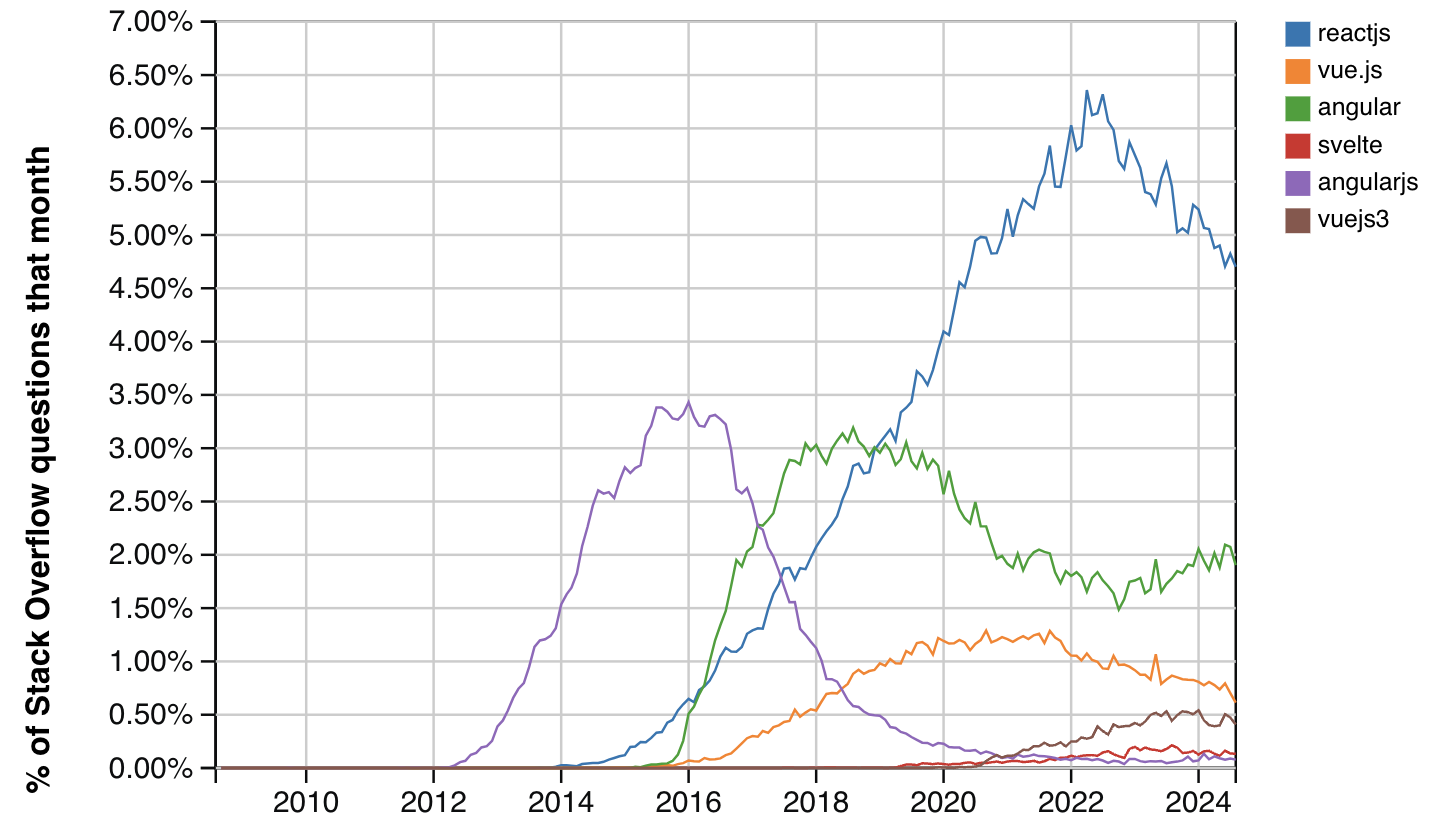
\includegraphics[width=10cm]{Images/react-stack-overflow.png}
                \vspace{0.5cm}
                \caption{Đồ thị phần trăm việc sử dụng tag tên trên Stackoverflow. Truy cập ngày: 13/02/2025}
                \label{fig:my_label}
            \end{figure}

            \textbf{Kết luận: } Dựa trên các bảng so sánh, nhóm quyết định chọn ReactJS là công nghệ chính để phát triển giao diện người dùng vì các lý do sau:

            \begin{itemize}
                \item Phù hợp với quy mô dự án: ReactJS không yêu cầu cấu trúc quá phức tạp như Angular, rất phù hợp với các dự án vừa và nhỏ. Điều này cho phép nhóm tập trung vào tính năng chính, như giao diện đặt món, mà không bị phân tâm vào các chi tiết kỹ thuật phức tạp.
                \item Sự quen thuộc: Việc đã có kinh nghiệm với ReactJS giúp nhóm phát triển hệ thống nhanh chóng hơn, đồng thời có thể tận dụng cộng đồng hỗ trợ lớn từ ReactJS.
            \end{itemize}
            % Dựa trên số liệu từ tháng 1 năm 2020 đến tháng 7 năm 2022, React đã thể hiện sự thống trị vượt trội trong cộng đồng phát triển frontend. Sự phổ biến của React được thể hiện qua số lượng repository phụ thuộc vào nó trên GitHub, vượt xa so với các framework khác như Vue và Angular 2+. Cụ thể, React đã đạt hơn 200.000 lượt sao trên GitHub, trong khi Vue và Angular còn chưa tới 100.000 lượt sao trên GitHub.

            % \begin{figure}[H]
            %     \centering
            %     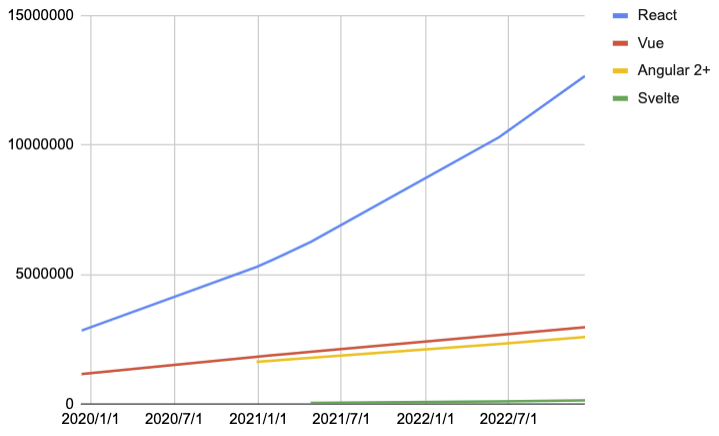
\includegraphics[width=10cm]{Images/react-repository.png}
            %     \vspace{0.5cm}
            %     \caption{Biểu đồ đường số lượng repository sử dụng framework}
            %     \label{fig:my_label}
            % \end{figure}

            % \begin{figure}[H]
            %     \centering
            %     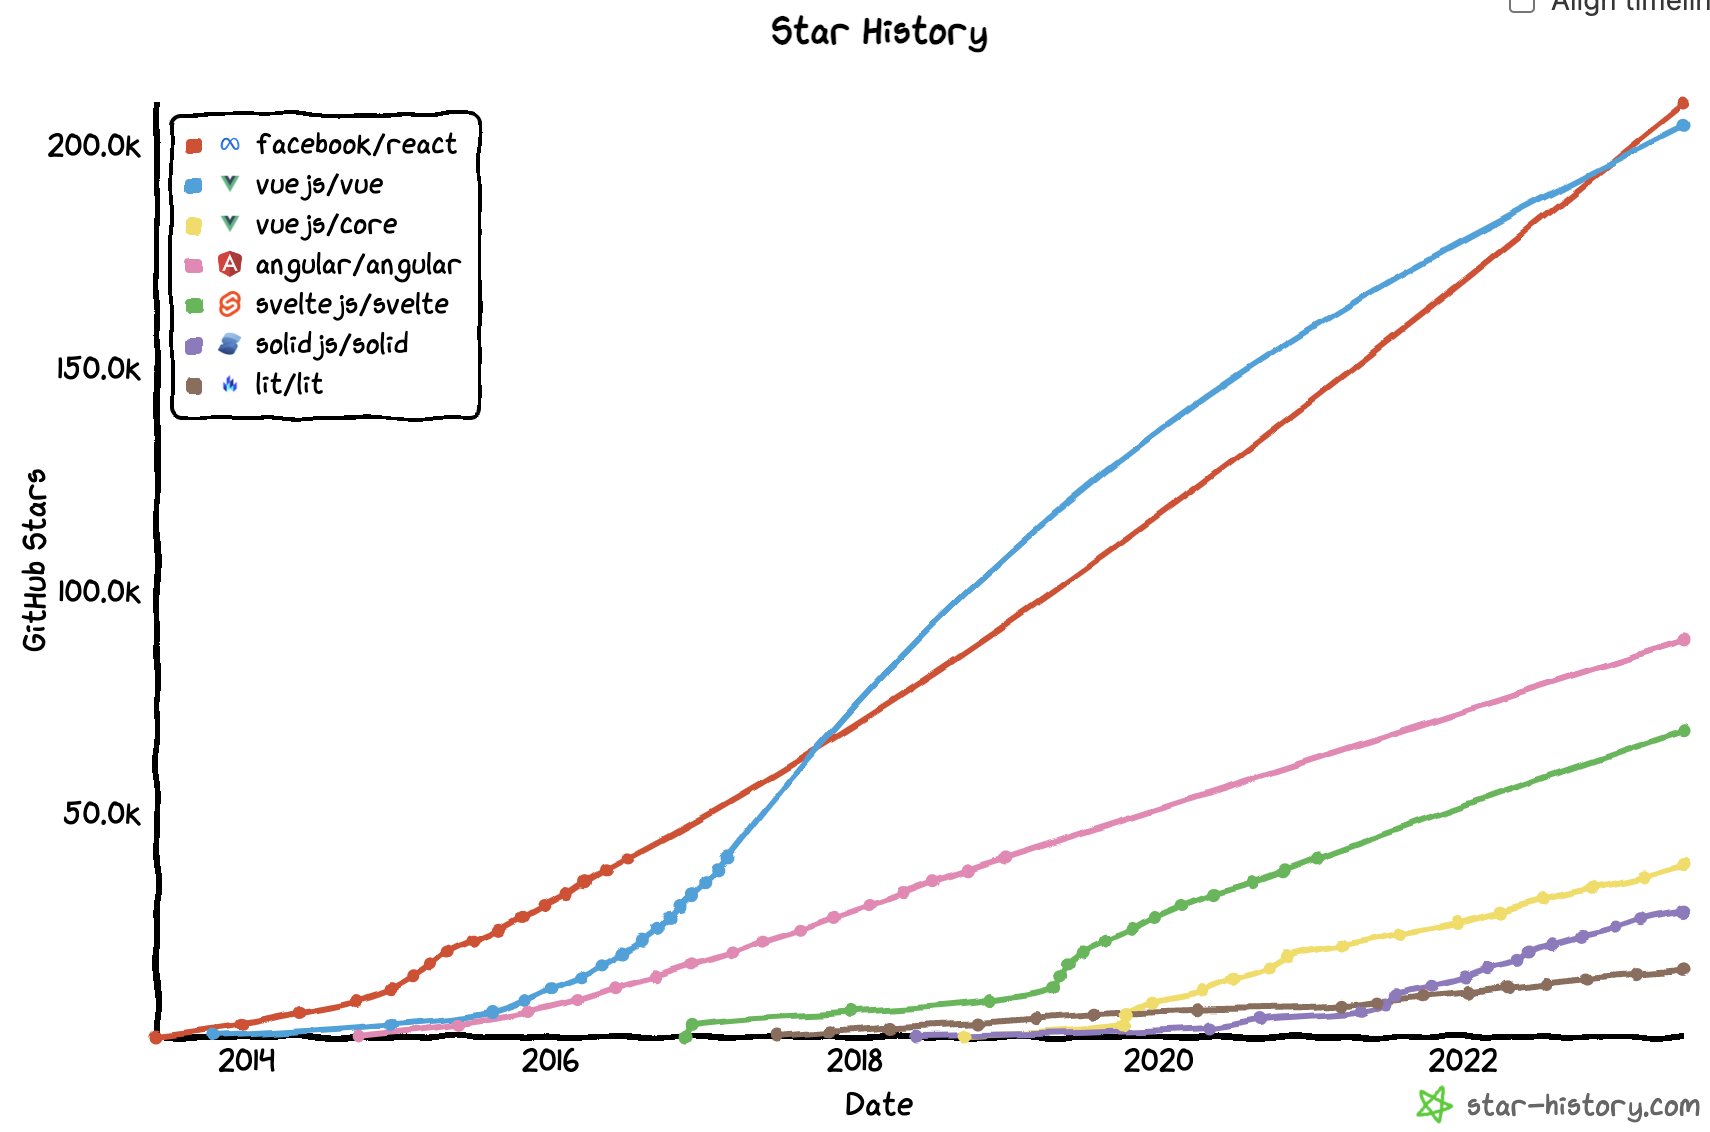
\includegraphics[width=10cm]{Images/react-star-history.png}
            %     \vspace{0.5cm}
            %     \caption{Biểu đồ thống kê GitHub Stars các framework phổ biến}
            %     \label{fig:my_label}
            % \end{figure}
            
            % Và còn nhiều kết quả thống kê khác đều chứng minh React luôn đi đầu trong số các Frontend framework khác như Vue, Angular hay Svelte \cite{FrontendFrameworks}. 
        
        % \item \textit{Nhược điểm}
        % \begin{itemize}
        %     \item \textbf{Vấn đề hiệu suất trên thiết bị cũ}: Ứng dụng React có thể gặp khó khăn trong việc duy trì hiệu suất trên các thiết bị cũ hoặc cấu hình thấp, do việc sử dụng Virtual DOM và các tính năng phức tạp có thể tiêu tốn tài nguyên hệ thống. 
        %     \item \textbf{Cập nhật thường xuyên}: React phát triển nhanh chóng, với các bản cập nhật và tính năng mới liên tục. Điều này có thể tạo ra gánh nặng cho các nhà phát triển trong việc duy trì và cập nhật mã nguồn để tương thích với các phiên bản mới.
        %     \item \textbf{JSX Learning Curve}: JSX, cú pháp kết hợp giữa JavaScript và HTML, có thể gây khó khăn cho những người mới bắt đầu, đặc biệt là khi làm quen với các khái niệm như state, props và lifecycle methods.
        % \end{itemize}
    \end{enumerate}

\subsubsubsection{ShadCN}
    \begin{enumerate}[(a)]
        \item \textit{Giới thiệu}

            ShadCN là một bộ sưu tập các thành phần giao diện người dùng (UI components) có thể tái sử dụng, được thiết kế đẹp mắt và dễ dàng tích hợp vào ứng dụng.

            Được xây dựng dựa trên thư viện Radix và framework Tailwind CSS, ShadCN cung cấp các thành phần như Button, Modal, Dropdown và nhiều hơn nữa, với khả năng tùy chỉnh linh hoạt để phù hợp với nhu cầu của từng dự án.

        \item \textit{Ưu điểm}

        \begin{itemize}
            \item \textbf{Thiết kế hướng đến doanh nghiệp}: ShadCN tập trung vào giao diện người dùng sạch sẽ và chuyên nghiệp, phù hợp cho các công cụ nội bộ và các ứng dụng nghiêm túc.
            \item \textbf{Tích hợp dễ dàng với React}: ShadCN UI được xây dựng đặc biệt cho React, giúp việc tích hợp và sử dụng trong các dự án React trở nên đơn giản và trực quan hơn. Điều này giúp giảm thiểu thời gian học tập và triển khai cho các nhà phát triển React.
            \item \textbf{Hiệu suất tối ưu}: Thư viện được thiết kế để tối ưu hóa hiệu suất, giúp giảm thiểu kích thước gói và tăng tốc độ tải trang. Điều này đặc biệt quan trọng trong các ứng dụng web hiện đại, nơi hiệu suất là yếu tố quan trọng.
        \end{itemize}

        \item \textit{Vì sao chọn ShadCN} 

            Nhóm quyết định chọn ShadCN để phát triển hệ thống Menu+ vì những lý do chính sau:

            \begin{itemize}
                \item Giao diện đồng nhất: ShadCN giúp hệ thống có giao diện đẹp, chuyên nghiệp và nhất quán, mang lại trải nghiệm mượt mà cho người dùng.
                \item Tăng tốc phát triển front-end: Với các thành phần UI đã được thiết kế sẵn, ShadCN giúp giảm thời gian phát triển, cho phép tập trung vào chức năng chính của hệ thống. Bên cạnh đó, nó còn hỗ trợ tính năng responsive, đảm bảo trải nghiệm người dùng trên mọi nền tảng.
                \item Tùy chỉnh dễ dàng: ShadCN cho phép tùy biến giao diện linh hoạt, giúp hệ thống có thể thay đổi theo nhu cầu và yêu cầu cụ thể.
            \end{itemize}

            Về mặt sử dụng, ShadCN hiện đang được sử dụng bởi khoảng 11.395 trang web, trong đó có 14 trang web nằm trong top 10 nghìn.

            \begin{figure}[H]
                \centering
                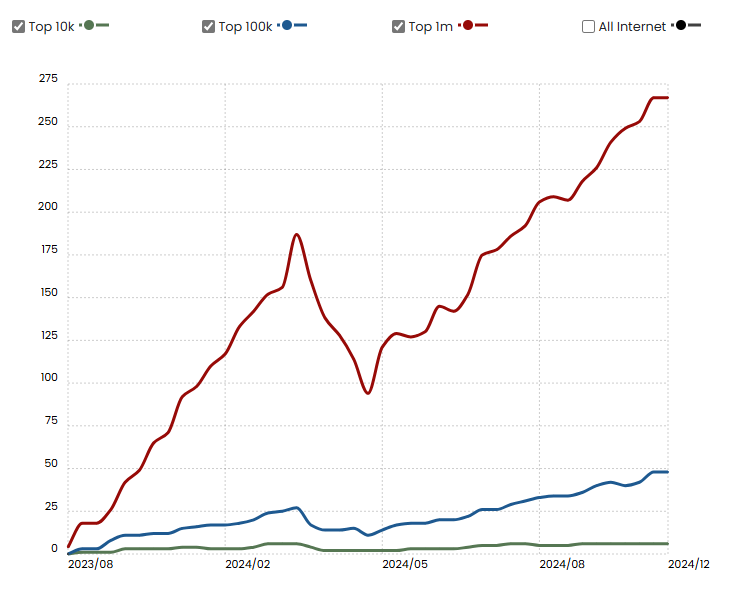
\includegraphics[width=10cm]{Images/shadcn-stats.png}
                \vspace{0.5cm}
                \caption{Thống kê sử dụng shadcn ui \cite{ShadcnUI}}
                \label{fig:my_label}
            \end{figure}
            
        % \item \textit{Nhược điểm}

        % \begin{itemize}
        %     \item \textbf{Thiếu cộng đồng lớn}: So với các thư viện UI phổ biến như MUI, ShadCN UI có cộng đồng người dùng và nhà phát triển nhỏ hơn. Điều này có thể dẫn đến việc thiếu tài liệu hỗ trợ và ít giải pháp cho các vấn đề thường gặp.
        %     \item \textbf{Hạn chế về thành phần giao diện}: Mặc dù ShadCN UI cung cấp nhiều thành phần cơ bản, nhưng so với MUI, thư viện này có thể thiếu một số thành phần phức tạp hoặc đặc biệt, điều này có thể yêu cầu bạn tự phát triển hoặc tích hợp thêm các thư viện khác.
        % \end{itemize}
    \end{enumerate}

\subsubsubsection{TanStack}
    \begin{enumerate}[(a)]
        \item \textit{Giới thiệu}

            TanStack là một tập hợp các thư viện mã nguồn mở chất lượng cao, được thiết kế để hỗ trợ các nhà phát triển web trong việc xây dựng ứng dụng hiệu quả và mạnh mẽ. Các thư viện của TanStack tập trung vào việc cung cấp các tiện ích "headless" (không có giao diện mặc định), an toàn về kiểu dữ liệu và mạnh mẽ cho các tác vụ như quản lý trạng thái, định tuyến, hiển thị dữ liệu và hơn thế nữa.

            TanStack cam kết cung cấp các công cụ mạnh mẽ và linh hoạt, giúp các nhà phát triển tạo ra các ứng dụng web hiệu quả và dễ bảo trì. Với triết lý "headless", các thư viện của TanStack cho phép tùy chỉnh giao diện hoàn toàn, dễ dàng tích hợp vào bất kỳ dự án nào mà không bị ràng buộc bởi các thiết kế mặc định \cite{TanStack}.
        
        \item \textit{Ưu điểm}

        \begin{itemize}
            \item \textbf{Quản lý trạng thái máy chủ hiệu quả}: TanStack Query (trước đây là React Query) giúp quản lý trạng thái bất đồng bộ trong React, đặc biệt trong việc fetching, caching và đồng bộ hóa dữ liệu từ server. Điều này giúp cải thiện hiệu suất và trải nghiệm người dùng.
            \item \textbf{Tối ưu hóa hiệu suất}: Với cơ chế caching tự động, TanStack giảm tải cho server và tăng tốc độ phản hồi của ứng dụng. Dữ liệu được lưu trữ trong bộ nhớ đệm và cập nhật nền, đảm bảo người dùng luôn có thông tin mới nhất mà không cần thực hiện các yêu cầu API không cần thiết. 
            \item \textbf{Xử lý lỗi và quản lý truy vấn dễ dàng}: TanStack cung cấp cách tiếp cận rõ ràng và nhất quán để xử lý lỗi, bao gồm khả năng tự động thử lại các truy vấn HTTP thất bại. Ngoài ra, việc quản lý truy vấn trở nên dễ dàng hơn với các tính năng như nhóm truy vấn, vô hiệu hóa và tìm nạp lại khi cần thiết.
        \end{itemize}

        \item \textit{Vì sao chọn TanStack} 

            TanStack được chọn để phát triển hệ thống Menu+ bởi các lí do chính sau:
            \begin{itemize}
                \item Quản lý trạng thái hiệu quả: TanStack giúp đồng bộ dữ liệu giữa các trang như thực đơn, đơn hàng, và thông tin khách hàng, đảm bảo trải nghiệm người dùng mượt mà. 
                \item Tối ưu hiệu suất: Tính năng caching và prefetching giúp giảm số lần gọi API, tăng tốc độ xử lý dữ liệu như thông tin món ăn, đơn hàng, và thanh toán.
                \item Xử lý truy vấn phức tạp: TanStack hỗ trợ việc tìm kiếm món ăn, lọc theo danh mục và theo dõi đơn hàng theo thời gian thực một cách hiệu quả và nhanh chóng.
            \end{itemize}

            Sự phổ biến của TanStack được minh chứng qua những con số ấn tượng sau:

            \begin{itemize}
                \item Hơn 1,7 tỷ lượt tải trên NPM, thể hiện sự tin dùng rộng rãi trong cộng đồng phát triển.
                \item 95,271 sao trên GitHub, chứng tỏ sự đánh giá cao từ lập trình viên trên toàn cầu.
                \item 2,142 người đóng góp trên GitHub, cho thấy cộng đồng phát triển mạnh mẽ và liên tục cải tiến.
                \item 837,561 dự án phụ thuộc trên GitHub, khẳng định mức độ tích hợp cao và ứng dụng thực tế rộng rãi.
            \end{itemize}
            
            \begin{figure}[H]
                \centering
                
\includegraphics[width=10cm]{Images/tanstack-stats.png}
                \vspace{0.5cm}
                \caption{Các số liệu thống kê về Tanstack \cite{TanStack}}
                \label{fig:my_label}
            \end{figure}
 
        % \item \textit{Nhược điểm}

        % \begin{itemize}
        %     \item \textbf{Quản lý bộ nhớ đệm phức tạp}: Việc quản lý tầng dữ liệu cache yêu cầu sự cẩn trọng; nếu không, có thể dẫn đến các lỗi không mong muốn trong ứng dụng. 
        %     \item \textbf{Phức tạp khi kết hợp với các thư viện khác}: Sử dụng TanStack song song với các thư viện quản lý trạng thái khác như Redux có thể gây ra sự phức tạp trong luồng mã và quản lý trạng thái.
        % \end{itemize}
        
    \end{enumerate}
\subsubsection{Công nghệ Back-end}
\subsubsubsection{SpringBoot}
\begin{enumerate}[(a)]
	\item \textit{Giới thiệu}

	      Spring Boot là một framework mã nguồn mở dựa trên nền tảng Java, được thiết kế để đơn giản hóa việc phát triển các ứng dụng Spring độc lập, sẵn sàng cho môi trường sản xuất. Nó cung cấp các cấu hình mặc định thông minh và tự động, giúp giảm thiểu cấu hình thủ công và tối ưu hóa quá trình phát triển ứng dụng Java. Spring Boot tích hợp tốt với nhiều công nghệ và thư viện khác trong hệ sinh thái Spring Framework, cho phép hệ thống dễ dàng tích hợp các module và dịch vụ khác nhau mà không cần phải lo lắng về cấu hình phức tạp. Ngoài ra, Spring Boot đi kèm với các máy chủ nhúng như Tomcat, Jetty hoặc Undertow, giúp triển khai ứng dụng một cách đơn giản mà không cần cấu hình thêm bất kỳ máy chủ nào khác

	\item \textit{Ưu điểm} \cite{SpringBootBenefits}

	      \begin{itemize}
		      \item \textbf{Phát triển nhanh chóng}: Tuân theo nguyên tắc "quy ước hơn cấu hình" (convention over configuration), Spring Boot cung cấp các thiết lập mặc định hợp lý cho các trường hợp sử dụng phổ biến. Cách tiếp cận này giúp giảm thiểu mã lặp (boilerplate code), cho phép lập trình viên tập trung vào logic nghiệp vụ thay vì phải cấu hình phức tạp.
		      \item \textbf{Tự động cấu hình}: Cơ chế tự động cấu hình (auto-configuration) của Spring Boot giúp thiết lập các thành phần ứng dụng dựa trên các thư viện và đặc điểm của dự án, giảm bớt công việc cấu hình thủ công và tối ưu hóa quy trình phát triển.
		      \item \textbf{Tích hợp liền mạch với hệ sinh thái Spring}: Spring Boot kết nối dễ dàng với các dự án khác trong hệ sinh thái Spring như Spring Data, Spring Security và Spring Cloud, cung cấp một nền tảng toàn diện để phát triển ứng dụng.
		      \item \textbf{Tính sẵn sàng cho môi trường sản xuất}: Spring Boot tích hợp sẵn các tính năng hỗ trợ triển khai trong môi trường thực tế như kiểm tra sức khỏe (health checks), thu thập số liệu (metrics), và cấu hình bên ngoài (externalized configuration), giúp giám sát và quản lý ứng dụng hiệu quả hơn.
	      \end{itemize}

	\item \textit{So sánh Spring Boot và các công nghệ khác}

	      Khi so sánh giữa các công nghệ liên quan, đặc biệt là Spring Boot với Express, Flask và Django, chúng ta có thể nhận thấy mỗi công nghệ có những ưu điểm và hạn chế riêng. Dưới đây là bảng so sánh chi tiết giữa Spring Boot và các công nghệ khác, dựa trên các tài liệu \cite{BackCompare1}, \cite{BackCompare2}, \cite{BackCompare3}:

	      \begin{landscape}  % Bắt đầu phần landscape
		      \begin{longtable}{|p{3.5cm}|p{5cm}|p{5cm}|p{5cm}|p{5cm}|}
			      \caption{Bảng so sánh các công nghệ Back-end phổ biến}
			      \hline
			      \textbf{Tiêu Chí}    & \textbf{Spring Boot}                                                         & \textbf{Express}                                                         & \textbf{Flask}                                           & \textbf{Django}                                           \\
			      \hline
			      \endfirsthead
			      \hline
			      \textbf{Tiêu Chí}    & \textbf{Spring Boot}                                                         & \textbf{Express}                                                         & \textbf{Flask}                                           & \textbf{Django}                                           \\
			      \hline
			      \endhead
			      \hline
			      Ngôn ngữ             & Java (hỗ trợ TypeScript qua tích hợp)                                        & JavaScript (hỗ trợ TypeScript)                                           & Python                                                   & Python                                                    \\
			      \hline
			      Định nghĩa           & Framework Java để xây dựng ứng dụng web và microservices                     & Môi trường runtime JavaScript với Express là framework nhẹ cho backend   & Framework Python nhẹ cho phát triển web                  & Framework Python toàn diện cho phát triển web             \\
			      \hline
			      Kiến trúc            & Dựa trên thành phần, MVC, tự động cấu hình, luồng dữ liệu một chiều          & Dựa trên sự kiện, không chặn (non-blocking), linh hoạt                   & Không áp đặt, linh hoạt, microframework                  & MVC (MTV - Model-Template-View), tích hợp sẵn             \\
			      \hline
			      Thời gian phát triển & Nhanh cho dự án lớn nhờ tự động cấu hình, chậm hơn cho dự án nhỏ             & Rất nhanh, đặc biệt cho ứng dụng nhỏ và thời gian đưa ra thị trường ngắn & Rất nhanh cho dự án nhỏ, cần thêm cấu hình cho dự án lớn & Nhanh, tích hợp sẵn nhiều tính năng                       \\
			      \hline
			      Độ phức tạp          & Trung bình đến cao, cần hiểu Spring ecosystem                                & Thấp, dễ bắt đầu nhưng phức tạp hơn khi mở rộng quy mô                   & Thấp, đơn giản nhưng phức tạp khi mở rộng                & Trung bình, dễ dùng nhưng phức tạp với tùy chỉnh nâng cao \\
			      \hline
			      Tính linh hoạt       & Trung bình, bị ràng buộc bởi cấu trúc Spring nhưng dễ tích hợp thư viện Java & Cao, tự do chọn công cụ và thư viện                                      & Cao, tự do chọn công cụ và cấu hình                      & Thấp hơn, bị ràng buộc bởi cấu trúc Django                \\
			      \hline
			      Bảo trì              & Dễ bảo trì cho ứng dụng lớn, khó hơn nếu không tổ chức tốt                   & Dễ bảo trì cho ứng dụng nhỏ, khó hơn khi codebase lớn                    & Dễ cho ứng dụng nhỏ, khó hơn khi codebase lớn            & Dễ bảo trì nhờ ORM và cấu trúc rõ ràng                    \\
			      \hline
			      Dễ sử dụng/Dễ học    & Khó hơn, cần kiến thức Java và Spring                                        & Dễ học, đặc biệt với người biết JavaScript                               & Rất dễ học, tối giản, phù hợp người mới                  & Dễ học, tài liệu tốt, phù hợp người mới                   \\
			      \hline
			      Kiểm thử             & JUnit, Mockito, tích hợp sẵn nhưng cần cấu hình                              & Jest, Mocha, dễ thiết lập và linh hoạt                                   & unittest, pytest, dễ thiết lập                           & unittest, pytest, tích hợp tốt                            \\
			      \hline
		      \end{longtable}
	      \end{landscape}

	      \textbf{Kết luận: } Dựa trên các bảng so sánh, nhóm quyết định chọn Spring Boot là công nghệ chính để phát triển hệ thống vì các lý do sau:

	      \begin{itemize}
		      \item Phù hợp với kiến trúc MVC: Spring Boot hỗ trợ tốt kiến trúc MVC (Model-View-Controller), giúp phân chia rõ ràng các phần của hệ thống và tạo cấu trúc dễ hiểu, phù hợp với yêu cầu đồ án. Điều này sẽ giúp nhóm triển khai hệ thống có tổ chức và dễ dàng phân chia công việc.
		      \item Linh hoạt và dễ mở rộng: Spring Boot mang lại khả năng tích hợp microservices và hỗ trợ các thư viện Java phong phú. Điều này cho phép nhóm dễ dàng mở rộng hệ thống trong tương lai mà không cần thay đổi quá nhiều mã nguồn.
		      \item Dễ bảo trì: Với cấu trúc dự án rõ ràng và các công cụ như Spring Boot Actuator, Spring Boot giúp nhóm dễ dàng theo dõi và bảo trì hệ thống, rất thuận lợi khi cần sửa lỗi nhanh chóng hoặc thực hiện các thay đổi trong quá trình phát triển.
	      \end{itemize}

\end{enumerate}

\subsubsubsection{Hibernate}
\begin{enumerate}[(a)]
	\item \textit{Giới thiệu}

	      Hibernate là một framework ORM (Object-Relational Mapping) mạnh mẽ dành cho Java, giúp lập trình viên làm việc với cơ sở dữ liệu một cách hiệu quả hơn. Nó cung cấp một lớp trừu tượng giữa ứng dụng và cơ sở dữ liệu, cho phép thao tác dữ liệu bằng các đối tượng Java thay vì truy vấn SQL thuần túy. Hibernate hỗ trợ nhiều hệ quản trị cơ sở dữ liệu khác nhau và có khả năng tự động ánh xạ các bảng trong cơ sở dữ liệu thành các lớp Java thông qua tập hợp các quy tắc ánh xạ linh hoạt. Ngoài ra, Hibernate còn đi kèm với các tính năng như quản lý phiên làm việc (session management), bộ nhớ đệm (caching), và hỗ trợ giao dịch (transaction management), giúp tối ưu hóa hiệu suất và đơn giản hóa quá trình phát triển ứng dụng. Với khả năng tích hợp dễ dàng cùng các framework khác như Spring và Java EE, Hibernate đã trở thành một trong những lựa chọn phổ biến nhất trong các ứng dụng doanh nghiệp sử dụng Java.

	\item \textit{Ưu điểm}

	      \begin{itemize}
		      \item \textbf{Ánh xạ đối tượng-quan hệ tự động}: Hibernate cho phép ánh xạ tự động giữa các lớp Java và các bảng trong cơ sở dữ liệu thông qua các tệp cấu hình XML hoặc annotation, giúp giảm thiểu mã nguồn và đơn giản hóa việc quản lý dữ liệu.
		      \item \textbf{Độc lập với cơ sở dữ liệu}: Mã lệnh của Hibernate có thể hoạt động với nhiều hệ quản trị cơ sở dữ liệu khác nhau như MySQL, Oracle mà không cần thay đổi mã HQL. Người dùng chỉ cần cập nhật thông tin cấu hình khi chuyển đổi hệ quản trị, giúp tiết kiệm thời gian và công sức.
		      \item \textbf{Quản lý phiên và giao dịch hiệu quả}: Hibernate cung cấp cơ chế quản lý phiên (Session) và giao dịch (Transaction) mạnh mẽ, đảm bảo tính toàn vẹn dữ liệu và hỗ trợ các thao tác như lưu trữ, cập nhật và xóa dữ liệu một cách an toàn.
		      \item \textbf{Hỗ trợ tải chậm (Lazy Loading)}: Hibernate hỗ trợ cơ chế tải chậm, chỉ tải dữ liệu khi cần thiết, giúp tiết kiệm tài nguyên hệ thống và cải thiện hiệu suất ứng dụng.

		      \item \textit{Vì sao chọn Hibernate}

		            Hibernate được chọn để phát triển hệ thống Menu+ vì những lý do sau:

		            \begin{itemize}
			            \item Quản lý dữ liệu đơn giản và hiệu quả: Menu+ cần quản lý lượng lớn dữ liệu như thực đơn, đơn hàng và thông tin khách hàng. Hibernate giúp ánh xạ tự động giữa các đối tượng trong Java và cơ sở dữ liệu, giúp giảm thiểu công việc thủ công trong việc viết mã SQL và làm cho việc quản lý dữ liệu trở nên dễ dàng và linh hoạt.
			            \item Hỗ trợ mở rộng: Menu+ có thể phát triển và mở rộng trong tương lai, ví dụ như thêm nhiều tính năng mới hoặc thay đổi cơ sở dữ liệu. Hibernate hỗ trợ nhiều loại cơ sở dữ liệu khác nhau, cho phép hệ thống dễ dàng thay đổi hoặc nâng cấp mà không gặp khó khăn lớn.
		            \end{itemize}
	      \end{itemize}

	      % \item \textit{Nhược điểm}

	      % \begin{itemize}
	      %     \item \textbf{Không hỗ trợ tốt cho các truy vấn phức tạp}: Hibernate có thể gặp khó khăn khi xử lý các truy vấn SQL phức tạp, đặc biệt là những truy vấn yêu cầu tối ưu hóa cao hoặc sử dụng các tính năng đặc thù của hệ quản trị cơ sở dữ liệu. Trong những trường hợp này, lập trình viên có thể phải sử dụng truy vấn SQL gốc (native SQL), làm giảm tính trừu tượng và lợi ích của ORM.
	      %     \item \textbf{Tăng độ trễ khởi tạo}: Việc sử dụng Hibernate có thể dẫn đến thời gian khởi tạo đối tượng và kết nối cơ sở dữ liệu lâu hơn so với cách viết SQL trực tiếp, do quá trình ánh xạ và cấu hình phức tạp.
	      %     \item \textbf{Tiêu thụ tài nguyên hệ thống}: Hibernate có thể tiêu thụ nhiều tài nguyên hệ thống hơn so với việc sử dụng JDBC thuần túy, đặc biệt khi không được cấu hình và tối ưu hóa đúng cách.
	      % \end{itemize}
\end{enumerate}

\subsubsubsection{Redis}
\begin{enumerate}[(a)]
	\item \textit{Giới thiệu}

	      Redis, viết tắt của "Remote Dictionary Server", là một hệ thống lưu trữ dữ liệu mã nguồn mở, hoạt động trong bộ nhớ (in-memory), thuộc loại NoSQL và sử dụng mô hình key-value. Được phát triển bởi Salvatore Sanfilippo vào năm 2009, Redis ban đầu được thiết kế để cải thiện khả năng mở rộng cho một dự án phân tích nhật ký web theo thời gian thực. Kể từ đó, nó đã trở thành một trong những cơ sở dữ liệu NoSQL phổ biến nhất, được sử dụng rộng rãi trong các ứng dụng yêu cầu hiệu suất cao và độ trễ thấp.

	      Redis lưu trữ toàn bộ dữ liệu trong bộ nhớ, cho phép truy xuất và ghi dữ liệu với tốc độ rất nhanh. Ngoài việc hỗ trợ các kiểu dữ liệu đơn giản như chuỗi (strings), Redis còn hỗ trợ các cấu trúc dữ liệu phức tạp như danh sách (lists), tập hợp (sets), tập hợp có thứ tự (sorted sets), băm (hashes), và nhiều cấu trúc khác. Điều này giúp Redis linh hoạt trong việc giải quyết nhiều bài toán khác nhau, từ lưu trữ phiên làm việc (session storage), hàng đợi tin nhắn (message queues), đến bộ đệm (caching) và phân tích thời gian thực.

	      Hiện nay, Redis được sử dụng bởi nhiều công ty lớn như Twitter, Airbnb, Tinder, Yahoo, Adobe, Hulu, Amazon và OpenAI, nhờ vào khả năng cung cấp hiệu suất cao và linh hoạt trong nhiều trường hợp sử dụng khác nhau.

	      \begin{figure}[H]
		      \centering
		      
\includegraphics[width=15cm]{Images/redis.png}
		      \vspace{0.5cm}
		      \caption{Logo của Redis}
		      \label{fig:my_label}
	      \end{figure}

	\item \textit{Ưu điểm} \cite{Redis}

	      \begin{itemize}
		      \item \textbf{Hiệu suất cao}: Là một hệ thống lưu trữ dữ liệu trong bộ nhớ (in-memory data store), Redis cung cấp các thao tác đọc và ghi cực kỳ nhanh chóng, có thể xử lý hàng triệu yêu cầu mỗi giây. Điều này làm cho Redis trở nên lý tưởng cho các ứng dụng yêu cầu truy cập dữ liệu với độ trễ thấp.
		      \item \textbf{Hỗ trợ đa dạng cấu trúc dữ liệu}: Redis hỗ trợ nhiều kiểu dữ liệu khác nhau, bao gồm chuỗi (strings), danh sách (lists), băm (hashes), tập hợp (sets) và tập hợp có thứ tự (sorted sets), cho phép các nhà phát triển triển khai hiệu quả nhiều chức năng khác nhau.
		      \item \textbf{Hệ thống nhắn tin xuất bản/đăng ký (Publish/Subscribe)}: Redis bao gồm một hệ thống nhắn tin xuất bản/đăng ký (Pub/Sub), cho phép giao tiếp theo thời gian thực giữa các ứng dụng, hữu ích cho việc xây dựng các hệ thống trò chuyện, thông báo và các tính năng thời gian thực khác.
	      \end{itemize}

	\item \textit{Vì sao chọn Redis}

	      Redis được chọn để phát triển hệ thống Menu+ vì những lý do sau:

	      \begin{itemize}
		      \item Tăng tốc độ truy xuất dữ liệu: Redis là một cơ sở dữ liệu lưu trữ theo kiểu key-value trong bộ nhớ (in-memory), giúp truy xuất dữ liệu cực kỳ nhanh chóng. Điều này rất quan trọng trong hệ thống Menu+ khi cần xử lý nhanh các tác vụ như lưu trữ thông tin đơn hàng, phiên làm việc của người dùng hay các trạng thái tạm thời.
		      \item Quản lý phiên làm việc (Session Management): Trong hệ thống quản lý đặt món, Redis rất hữu ích để lưu trữ và quản lý phiên làm việc của người dùng. Điều này giúp theo dõi trạng thái đăng nhập và các hoạt động của người dùng một cách hiệu quả, đồng thời giảm thiểu việc truy xuất cơ sở dữ liệu truyền thống.
		      \item Dễ dàng tích hợp: Redis có thể dễ dàng tích hợp vào hệ thống hiện tại của Menu+ mà không yêu cầu thay đổi lớn về cấu trúc. Nó cũng tương thích tốt với các hệ thống khác như Hibernate và TanStack, giúp cải thiện hiệu quả hoạt động của toàn bộ hệ thống.
	      \end{itemize}

	      % \item \textit{Nhược điểm}

	      % \begin{itemize}
	      %     \item \textbf{Giới hạn về dung lượng bộ nhớ}: Redis lưu trữ toàn bộ dữ liệu trong bộ nhớ RAM, do đó, khả năng lưu trữ bị giới hạn bởi dung lượng bộ nhớ vật lý của hệ thống. Đối với các ứng dụng yêu cầu lưu trữ lượng dữ liệu lớn, việc sử dụng Redis có thể dẫn đến chi phí cao và không khả thi. 
	      %     \item \textbf{Thiếu tính nhất quán mạnh mẽ}: Redis sử dụng mô hình sao chép bất đồng bộ, điều này có thể dẫn đến tình trạng dữ liệu không nhất quán giữa các nút chủ và nút phụ, đặc biệt trong các tình huống chuyển đổi dự phòng hoặc phân tách mạng.
	      %     \item \textbf{Hạn chế trong truy vấn phức tạp}: Redis không hỗ trợ các truy vấn phức tạp như join hoặc các phép tổng hợp, điều này làm giảm tính linh hoạt khi cần thao tác với dữ liệu phức tạp.
	      %     \item \textbf{Phức tạp trong việc thiết lập phân cụm}: Việc cấu hình và quản lý Redis Cluster có thể phức tạp, đòi hỏi kiến thức chuyên sâu và kinh nghiệm để đảm bảo hệ thống hoạt động ổn định và hiệu quả.
	      % \end{itemize}
\end{enumerate}

% \subsubsubsection{Kafka}
%     \begin{enumerate}[(a)]
%         \item \textit{Giới thiệu}

%         Apache Kafka là một nền tảng phân tán mã nguồn mở được thiết kế để xử lý các luồng dữ liệu theo thời gian thực. Ban đầu được phát triển bởi LinkedIn và sau đó trở thành dự án của Apache Software Foundation, Kafka cho phép các ứng dụng xuất bản, lưu trữ và tiêu thụ các luồng bản ghi (record streams) một cách hiệu quả. Hệ thống này hoạt động dựa trên mô hình xuất bản-đăng ký (publish-subscribe), trong đó các nhà sản xuất (producers) gửi thông điệp đến các chủ đề (topics), và các người tiêu thụ (consumers) đăng ký để nhận các thông điệp này. Kafka được sử dụng rộng rãi trong việc xây dựng các hệ thống xử lý dữ liệu thời gian thực, như theo dõi hoạt động người dùng, giám sát hệ thống, và phân tích dữ liệu trực tuyến. 

%         \begin{figure}[H]
%             \centering
%             \includegraphics[width=15cm]{Images/kafka.png}
%             \vspace{0.5cm}
%             \caption{Vị trí của Kafka trong dự án}
%             \label{fig:my_label}
%         \end{figure}
%         \item \textit{Ưu điểm}

%         \begin{itemize}
%             \item \textbf{Hiệu suất cao}: Kafka có khả năng xử lý lượng lớn thông tin với thông lượng cao và độ trễ thấp, cho phép xử lý hàng triệu thông điệp mỗi giây.
%             \item \textbf{Khả năng mở rộng}: Với kiến trúc phân tán, Kafka dễ dàng mở rộng bằng cách thêm các broker vào cụm, tăng khả năng xử lý dữ liệu mà không cần thay đổi cấu trúc hệ thống. 
%             \item \textbf{Độ tin cậy và bền vững}: Kafka lưu trữ các sự kiện theo định dạng nhật ký đơn giản, đảm bảo dữ liệu bền vững và chính sách lưu giữ dễ triển khai. 
%             \item \textbf{Xử lý dữ liệu thời gian thực}: Kafka được thiết kế để xử lý dữ liệu thời gian thực và streaming, cho phép bạn đáp ứng nhanh chóng đối với sự kiện mới xảy ra. 
%         \end{itemize}

%         % \item \textit{Nhược điểm}

%         % \begin{itemize}
%         %     \item \textbf{Phức tạp trong cài đặt và quản lý}: Việc triển khai và cấu hình Kafka ban đầu có thể phức tạp, đặc biệt đối với những người mới bắt đầu. Để quản lý hiệu quả, cần có kiến thức sâu về hệ thống phân tán và mạng.
%         %     \item \textbf{Yêu cầu tài nguyên hệ thống cao}: Kafka đòi hỏi một lượng tài nguyên phần cứng đáng kể, bao gồm bộ nhớ, dung lượng lưu trữ và khả năng xử lý, để hoạt động hiệu quả. 
%         %     \item \textbf{Thiếu công cụ giám sát hoàn chỉnh}: Kafka không cung cấp một bộ công cụ giám sát và quản lý tích hợp đầy đủ. Người dùng thường phải dựa vào các công cụ của bên thứ ba để theo dõi và quản lý hệ thống.
%         % \end{itemize}
%     \end{enumerate}

% % \subsubsubsection{RESTful API}
% %     \begin{enumerate}[(a)]
% %         \item \textit{Giới thiệu}

% %         \item \textit{Vì sao chọn RESTful API} 

% %         \item \textit{Ưu điểm}

% %         \item \textit{Nhược điểm}
% %     \end{enumerate}
\subsubsection{Cơ sở dữ liệu - PostgreSQL}
    \begin{enumerate}[(a)]
        \item \textit{Giới thiệu}
        
            PostgreSQL là một hệ thống quản lý cơ sở dữ liệu quan hệ đối tượng (ORDBMS) mã nguồn mở, được phát triển từ năm 1986 tại Đại học California, Berkeley, dưới sự dẫn dắt của giáo sư Michael Stonebraker. Ban đầu, nó được gọi là "Postgres" và đã trải qua nhiều giai đoạn phát triển để trở thành một trong những hệ quản trị cơ sở dữ liệu phổ biến nhất hiện nay. 

            PostgreSQL hỗ trợ cả truy vấn SQL truyền thống và JSON, cho phép xử lý linh hoạt cả dữ liệu quan hệ và phi quan hệ. Nó cung cấp các tính năng nâng cao như hỗ trợ các kiểu dữ liệu đa dạng, khả năng mở rộng cao và tuân thủ các tiêu chuẩn SQL mới nhất.

            Ngày nay, PostgreSQL được sử dụng rộng rãi trong nhiều lĩnh vực, từ các ứng dụng web động đến các hệ thống thông tin địa lý, nhờ vào khả năng hỗ trợ các đối tượng địa lý và tính năng ghi nhật ký trước, giúp đảm bảo tính toàn vẹn và khả năng khôi phục dữ liệu.
                    
        \item \textit{Ưu điểm}

        \begin{itemize}
            \item \textbf{Xử lý khối lượng dữ liệu lớn}: PostgreSQL có khả năng quản lý các hệ thống lớn với hàng triệu bản ghi, đáp ứng nhu cầu của các tập đoàn và tổ chức yêu cầu hệ thống cơ sở dữ liệu mạnh mẽ và đáng tin cậy. 
            \item \textbf{Kiểm soát đồng thời nhiều phiên bản (MVCC)}: Tính năng MVCC cho phép PostgreSQL xử lý các thao tác ghi thường xuyên và truy vấn phức tạp một cách hiệu quả, phù hợp cho các ứng dụng cấp doanh nghiệp.
            \item \textbf{Độ tin cậy và phục hồi}: Sử dụng ghi nhật ký ghi trước (WAL), PostgreSQL đảm bảo độ tin cậy và hỗ trợ khôi phục điểm-theo-thời-gian (PITR) và active standbys, giúp hệ thống hoạt động ổn định và phục hồi nhanh chóng khi gặp sự cố.
        \end{itemize}

        \item \textit{So sánh PostgreSQL và các hệ quản trị cơ sở dữ liệu}
        
Khi so sánh PostgreSQL với các hệ quản trị cơ sở dữ liệu khác như MySQL, SQL Server và MongoDB, mỗi hệ thống đều sở hữu những đặc điểm nổi bật và phù hợp với các nhu cầu khác nhau. Dưới đây là bảng so sánh chi tiết giữa PostgreSQL và các cơ sở dữ liệu này, giúp làm rõ ưu điểm và hạn chế của từng loại.

\begin{landscape} 
\begin{longtable}{|p{3.5cm}|p{4cm}|p{4cm}|p{4cm}|p{4cm}|}
\hline
\textbf{Tiêu chí} & \textbf{PostgreSQL} & \textbf{MySQL} & \textbf{SQL Server} & \textbf{MongoDB} \\
\hline
\endfirsthead
\hline
\textbf{Tiêu chí} & \textbf{PostgreSQL} & \textbf{MySQL} & \textbf{SQL Server} & \textbf{MongoDB} \\
\hline
\endhead
\hline
\textbf{Loại cơ sở dữ liệu} & Quan hệ - Đối tượng (ORDBMS), mã nguồn mở & Quan hệ (RDBMS), mã nguồn mở & Quan hệ (RDBMS), độc quyền & Phi quan hệ (NoSQL), mã nguồn mở \\
\hline
\textbf{Hiệu suất} & Tốt cho truy vấn phức tạp, chậm hơn MySQL trong truy vấn đơn giản & Cao cho truy vấn đơn giản, ứng dụng web & Cao, tối ưu cho doanh nghiệp lớn & Cao cho dữ liệu phi cấu trúc, đọc/ghi nhanh \\
\hline
\textbf{Khả năng mở rộng} & Cao, hỗ trợ terabyte/petabyte dữ liệu & Tốt, hỗ trợ cluster và replication & Cao, tích hợp đám mây Azure & Rất cao, mở rộng ngang tốt \\
\hline
\textbf{Kiểu dữ liệu hỗ trợ} & Phong phú: JSON, XML, PostGIS, tùy chỉnh & Cơ bản, hỗ trợ JSON từ phiên bản 5.7 & Cơ bản, hỗ trợ XML, JSON & Linh hoạt: JSON, BSON \\
\hline
\textbf{Khả năng tìm kiếm văn bản} & Tìm kiếm văn bản đầy đủ, hỗ trợ ký tự quốc tế & Tìm kiếm văn bản cơ bản & Tìm kiếm văn bản tốt, tích hợp Full Text Search & Tìm kiếm văn bản tốt, tích hợp Atlas Search \\
\hline
\textbf{Hỗ trợ nền tảng} & Linux, Windows, macOS, Solaris & Linux, Windows, macOS & Chủ yếu Windows, hỗ trợ Linux & Linux, Windows, macOS \\
\hline
\textbf{Chi phí} & Miễn phí, mã nguồn mở & Miễn phí, có phiên bản thương mại & Độc quyền, chi phí cao & Miễn phí, có dịch vụ đám mây trả phí \\
\hline
\textbf{Ứng dụng phù hợp} & GIS, tài chính, ứng dụng phức tạp & Ứng dụng web, WordPress, Joomla & Doanh nghiệp lớn, tích hợp Microsoft & Ứng dụng thời gian thực, dữ liệu lớn \\
\hline
\caption{Bảng so sánh PostgreSQL và các hệ quản trị cơ sở dữ liệu}
\end{longtable}
\end{landscape} 

    \end{enumerate}
\subsubsection{Công nghệ triển khai}
\subsubsubsection{GitHub Actions}
    \begin{enumerate}[(a)]
        \item \textit{Giới thiệu}

        GitHub Actions là một nền tảng tích hợp sẵn trong GitHub, được giới thiệu vào năm 2018, cho phép các nhà phát triển tự động hóa các quy trình trong vòng đời phát triển phần mềm trực tiếp trên kho lưu trữ của họ. Nó hỗ trợ việc xây dựng, kiểm thử và triển khai ứng dụng thông qua việc tạo ra các workflow (quy trình làm việc) được định nghĩa bằng tệp YAML \cite{Viblo}.

        GitHub Actions cung cấp một hệ sinh thái phong phú với nhiều actions (hành động) có sẵn từ cộng đồng, cho phép người dùng dễ dàng tích hợp các công cụ và dịch vụ bên ngoài vào quy trình làm việc của họ. Ngoài ra, nó hỗ trợ chạy trên nhiều hệ điều hành như Windows, macOS và Ubuntu, giúp kiểm thử ứng dụng trên các môi trường khác nhau \cite{Viblo}.

        Với GitHub Actions, các nhà phát triển có thể thiết lập các quy trình CI/CD (Continuous Integration/Continuous Deployment) một cách linh hoạt và hiệu quả, tự động hóa các tác vụ như xây dựng, kiểm thử và triển khai ứng dụng, từ đó nâng cao hiệu suất làm việc và chất lượng sản phẩm.

        \item \textit{Ưu điểm}

        \begin{itemize}
            \item \textbf{Tích hợp liền mạch với GitHub}: Là một tính năng gốc của nền tảng GitHub, GitHub Actions cho phép các nhà phát triển tự động hóa workflow trực tiếp trong kho lưu trữ của họ. Sự tích hợp chặt chẽ này giúp đơn giản hóa các tác vụ như build, test và deploy code mà không cần sử dụng các công cụ bên ngoài.
            \item \textbf{Marketplace phong phú}: GitHub Marketplace cung cấp hơn 10.000 actions được xây dựng sẵn, giúp các nhà phát triển dễ dàng tích hợp nhiều công cụ và dịch vụ vào workflow của họ. Thư viện rộng lớn này giúp đơn giản hóa quá trình thiết lập các pipeline phức tạp bằng cách cung cấp các thành phần có thể tái sử dụng \cite{GitHubActionsIntro}.
            \item \textbf{Tự động hóa linh hoạt}: GitHub Actions hỗ trợ workflow dựa trên sự kiện (event-driven workflows), cho phép tự động hóa theo phản hồi của các sự kiện trong kho lưu trữ, chẳng hạn như push, pull request hoặc issue creation. Tính linh hoạt này giúp các nhà phát triển tùy chỉnh workflow để phù hợp với yêu cầu cụ thể của dự án.
            \item \textbf{Hỗ trợ đa nền tảng}: GitHub Actions cung cấp runners cho môi trường Linux, Windows và macOS, cho phép các nhà phát triển test và deploy ứng dụng trên nhiều hệ điều hành khác nhau. Khả năng hỗ trợ đa nền tảng này giúp đảm bảo ứng dụng hoạt động ổn định trong các môi trường khác nhau \cite{GitHubActionsDocs}.
        \end{itemize}
        
        % \item \textit{Nhược điểm} \cite{GitHubActionsMerits}

        % \begin{itemize}
        %     \item \textbf{Độ phức tạp trong workflow phức tạp}: Thiết kế workflow với nhiều bước và điều kiện có thể trở nên rối rắm, gây khó khăn trong việc bảo trì, đặc biệt đối với những người mới làm quen với các khái niệm về Continuous Integration/Continuous Deployment (CI/CD).
        %     \item \textbf{Giới hạn tài nguyên}: GitHub Actions áp đặt các giới hạn về mức sử dụng tài nguyên, bao gồm thời gian thực thi tối đa và dung lượng ổ đĩa có sẵn. Những hạn chế này có thể cản trở các workflow yêu cầu nhiều tài nguyên tính toán.
        %     \item \textbf{Phụ thuộc vào hệ sinh thái GitHub}: Do GitHub Actions được tích hợp chặt chẽ với nền tảng GitHub, bất kỳ sự cố gián đoạn hoặc downtime nào trên GitHub đều có thể ảnh hưởng trực tiếp đến các workflow CI/CD. Sự phụ thuộc này làm dấy lên lo ngại về độ tin cậy và khả năng sẵn sàng của hệ thống.
        %     \item \textbf{Thách thức trong quá trình debugging}: Việc xác định và khắc phục sự cố trong GitHub Actions có thể gặp khó khăn do khả năng quan sát (observability) và cơ chế phản hồi (feedback) còn hạn chế. Các nhà phát triển thường cần chèn nhiều log statement và chờ workflow thực thi để chẩn đoán vấn đề, dẫn đến chu kỳ phát triển kéo dài hơn.
        % \end{itemize}
    \end{enumerate}

\subsubsubsection{Docker}
    \begin{enumerate}[(a)]
        \item \textit{Giới thiệu}

        Docker là một nền tảng mã nguồn mở giúp các nhà phát triển tự động hóa việc triển khai, mở rộng và quản lý các ứng dụng trong các container nhẹ và di động. Các container này đóng gói ứng dụng và các phụ thuộc của nó, đảm bảo ứng dụng hoạt động nhất quán trên nhiều môi trường khác nhau.
        
        \item \textit{Ưu điểm} \cite{DockerAdvantages}

        \begin{itemize}
            \item \textbf{Tính di động và nhất quán}: Các container Docker đóng gói ứng dụng và các phụ thuộc của chúng, đảm bảo chúng chạy nhất quán trên nhiều môi trường khác nhau, từ phát triển đến sản xuất. Điều này loại bỏ vấn đề "it works on my machine" thường gặp. 
            \item \textbf{Hiệu quả tài nguyên}: Khác với các máy ảo truyền thống, các container Docker chia sẻ nhân hệ thống của máy chủ, giúp chúng nhẹ và hiệu quả hơn. Điều này cho phép khởi động nhanh hơn và chạy nhiều container hơn trên cùng một phần cứng, dẫn đến việc sử dụng tài nguyên tốt hơn. 
            \item \textbf{Triển khai nhanh chóng và khả năng mở rộng}: Docker cho phép triển khai và mở rộng ứng dụng một cách nhanh chóng. Các container có thể được khởi động hoặc dừng gần như ngay lập tức, tạo điều kiện cho việc mở rộng nhanh chóng dựa trên nhu cầu. Sự linh hoạt này rất quan trọng đối với các ứng dụng yêu cầu khả năng mở rộng động.
            \item \textbf{Tách biệt và bảo mật}: Docker cung cấp mức độ tách biệt cao giữa các ứng dụng, giảm thiểu rủi ro xung đột và tăng cường bảo mật. Mỗi container hoạt động độc lập, giảm thiểu tác động của các lỗ hổng và đảm bảo hiệu suất ứng dụng ổn định.
            \item \textbf{Quản lý phiên bản và hợp tác đơn giản}: Các image Docker có thể được quản lý phiên bản, cho phép các nhà phát triển theo dõi thay đổi và quay lại các trạng thái trước đó nếu cần. Quản lý phiên bản này đảm bảo tính nhất quán trên các giai đoạn khác nhau của vòng đời phát triển và tăng cường hợp tác giữa các nhóm phát triển.
        \end{itemize}
        
        % \item \textit{Nhược điểm}

        % \begin{itemize}
        %     \item \textbf{Hạn chế với ứng dụng GUI}: Docker chủ yếu hỗ trợ các ứng dụng dựa trên dòng lệnh và không phù hợp với các ứng dụng yêu cầu giao diện người dùng đồ họa phong phú. Việc chạy ứng dụng GUI trong Docker có thể gặp khó khăn và không được hỗ trợ tốt.
        %     \item \textbf{Phụ thuộc vào hệ điều hành Linux}: Docker hoạt động tốt nhất trên hệ điều hành Linux. Trên Windows và macOS, Docker cần sử dụng máy ảo Linux để chạy các container, điều này có thể ảnh hưởng đến hiệu suất và khả năng tương thích.
        %     \item \textbf{Quản lý tài nguyên phức tạp}: Việc chia sẻ tài nguyên giữa các container có thể dẫn đến xung đột hoặc giảm hiệu suất nếu không được quản lý đúng cách. Nếu một container chiếm dụng quá nhiều tài nguyên, nó có thể ảnh hưởng đến các container khác trên cùng hệ thống.
        % \end{itemize}
    \end{enumerate}
\subsection{Kiến trúc hệ thống}

\begin{figure}[H]
    \centering
    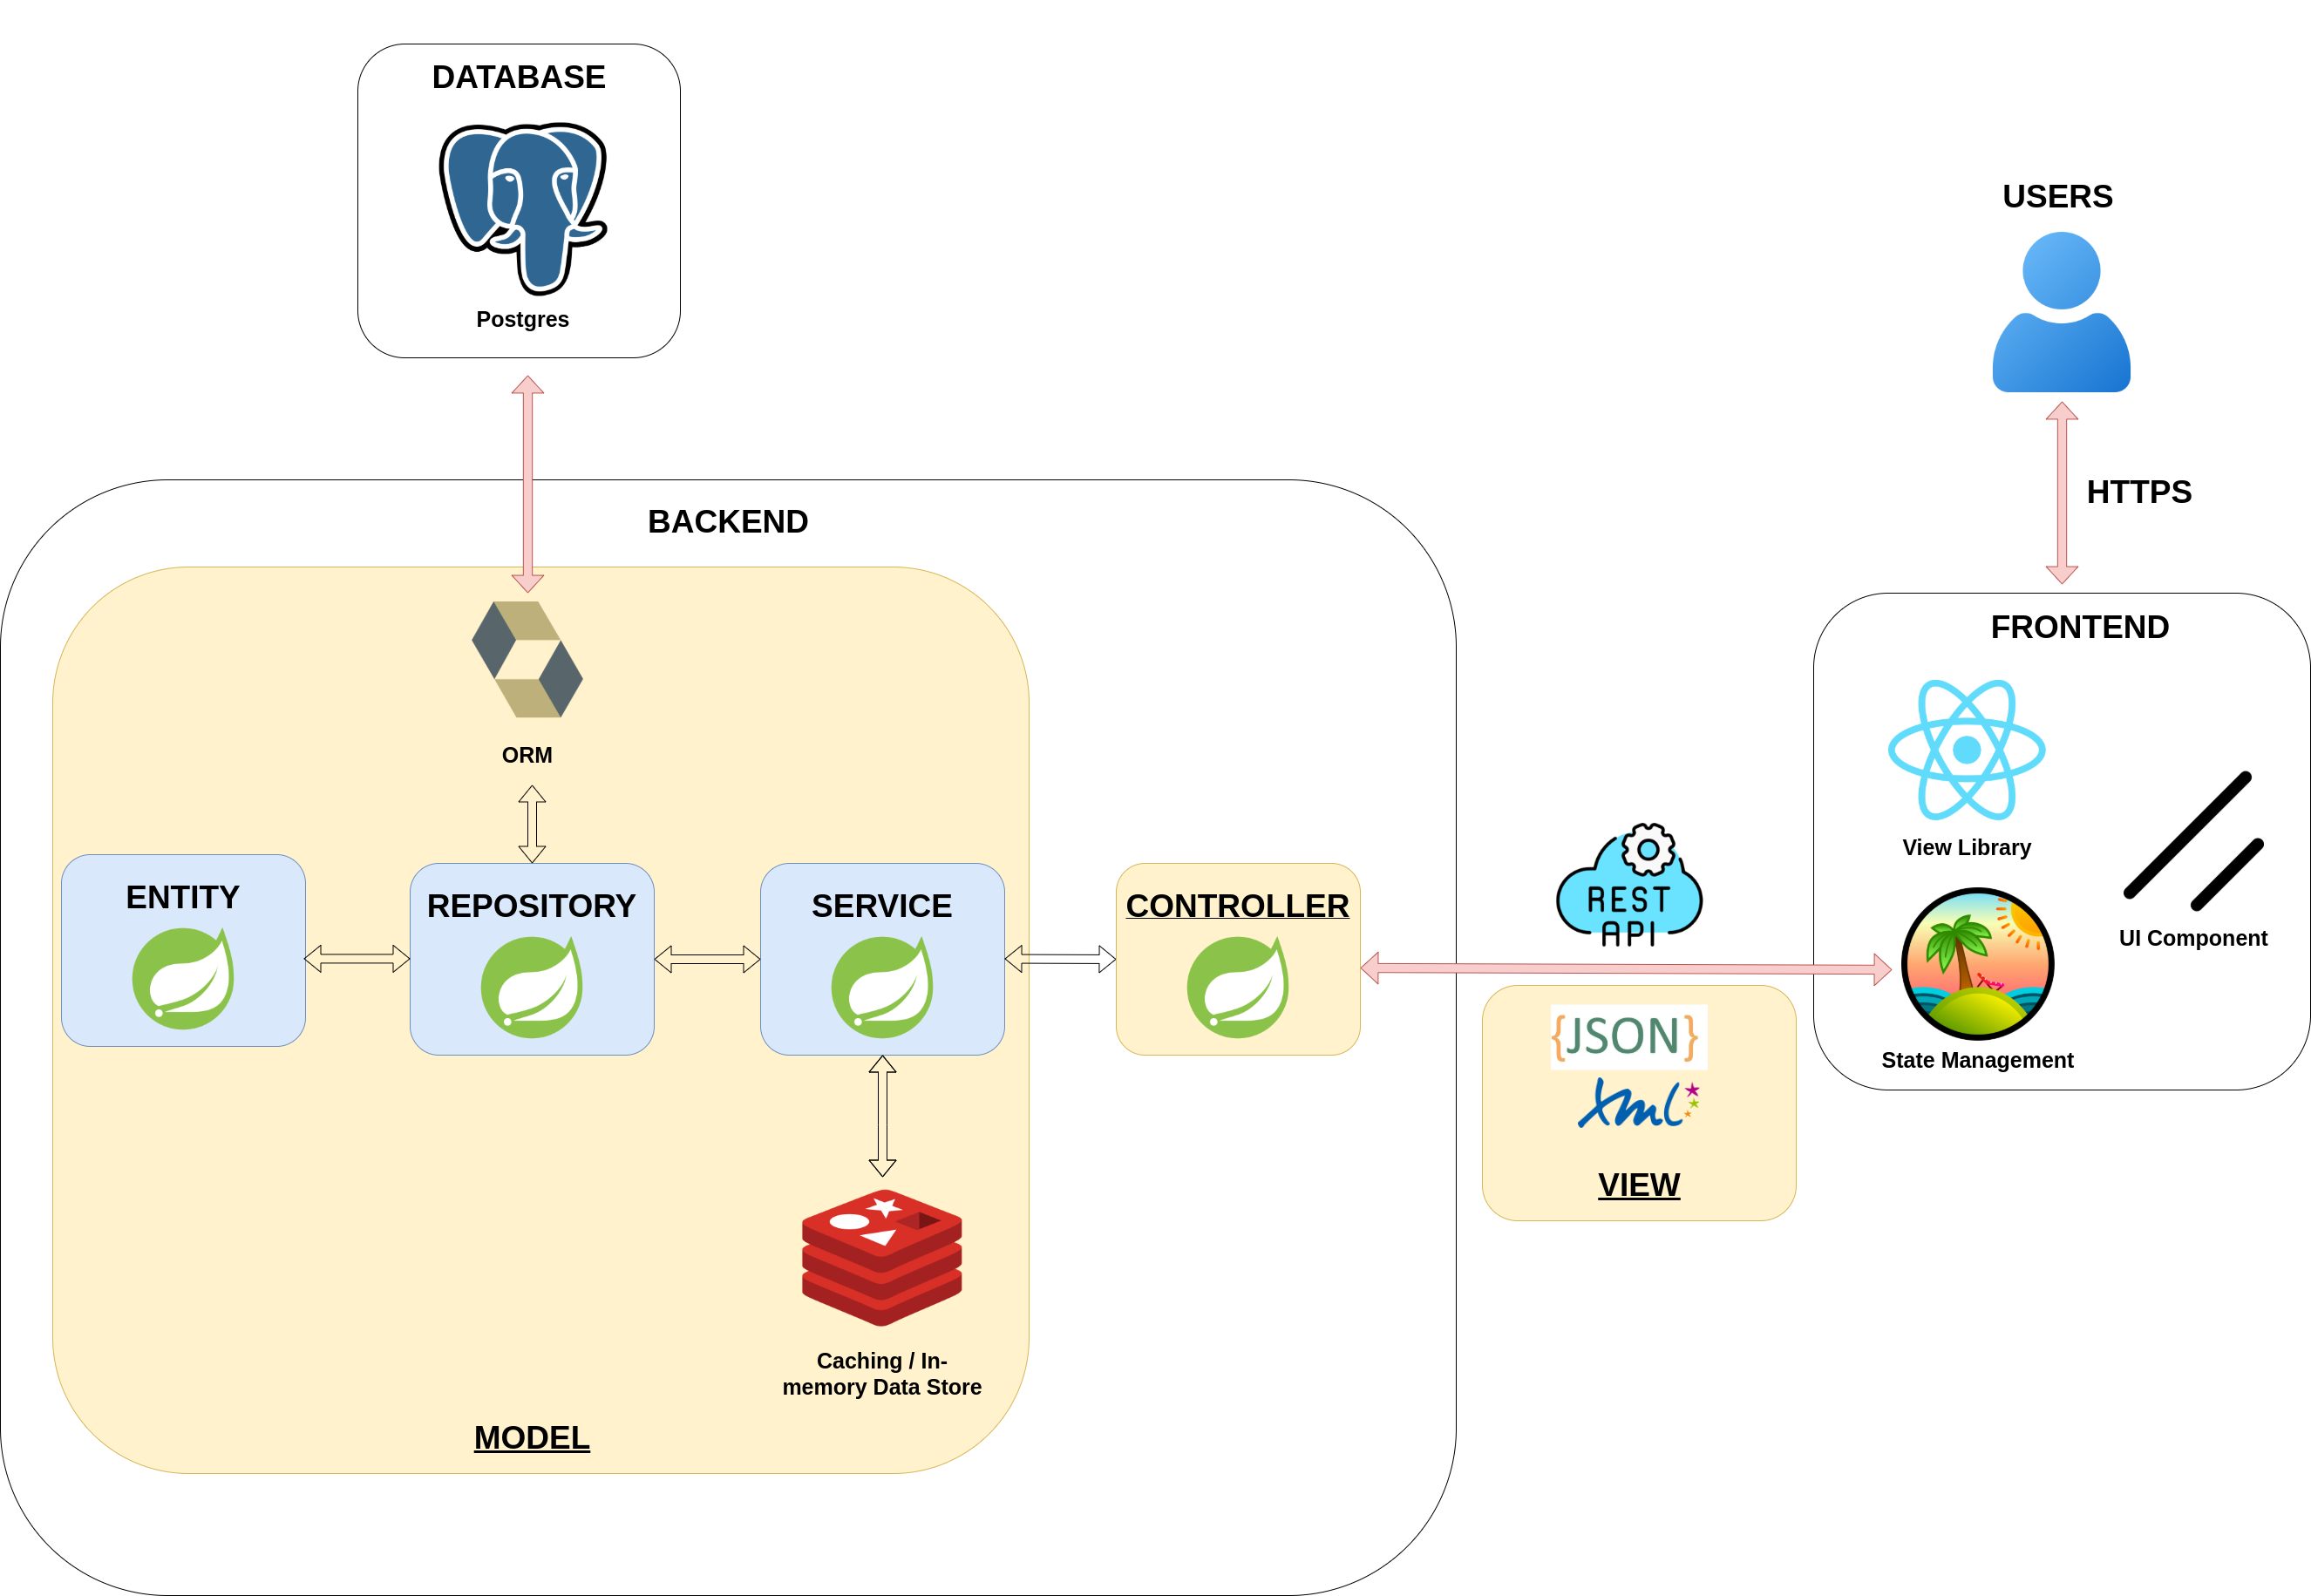
\includegraphics[width=10cm]{Images/kien-truc-he-thong.drawio.png}
    \vspace{0.5cm}
    \caption{Kiến trúc hệ thống}
    \label{fig:my_label}
\end{figure}

% Describing the importance of system architecture
Kiến trúc hệ thống đóng vai trò quan trọng trong dự án hệ thống quản lý nhà hàng. Nó xác định các thành phần chính của hệ thống và cách chúng tương tác với nhau để đáp ứng yêu cầu của người dùng. Kiến trúc này đảm bảo sự phân tách rõ ràng và sắp xếp logic giữa các thành phần, giúp dễ dàng quản lý, nâng cấp, mở rộng, tích hợp và tương tác giữa các thành phần khác nhau. Đồng thời, nó cung cấp khả năng mở rộng linh hoạt và thay đổi trong tương lai.

% Describing the architecture flow of the "Menu+" system
Dòng luồng kiến trúc của hệ thống "Menu+" được mô tả như sau:
\begin{itemize}
    \item Người dùng truy cập vào URL của hệ thống "Menu+" thông qua Internet.
    \item Khi truy cập, giao diện frontend của hệ thống được tải lên, bao gồm:
    \begin{itemize}
        \item Thư viện giao diện: ReactJS.
        \item Quản lý dữ liệu: TanStack.
        \item Thiết kế/Bố cục: ShadCN.
    \end{itemize}
    \item Nếu có hành động liên quan đến truy cập cơ sở dữ liệu hoặc dịch vụ bên thứ ba, hệ thống sử dụng TanStack để gửi yêu cầu đến server backend.
    \item Tại backend, Spring Boot Controller xử lý các yêu cầu API và ánh xạ chúng vào các URL tương ứng.
    \item Tiếp theo, tầng Service trong Spring Boot xác định hành động cần thực hiện dựa trên yêu cầu API.
    \item Nếu yêu cầu API cần truy cập cơ sở dữ liệu, Hibernate (ORM) sử dụng các entity để tạo truy vấn đến cơ sở dữ liệu PostgreSQL.
    \item Hibernate thực hiện truy vấn đến PostgreSQL, nơi lưu trữ dữ liệu của hệ thống.
    \item Để tối ưu hiệu suất, Service kiểm tra dữ liệu trong Redis (Caching/In-memory Data Store) trước; nếu không có, hệ thống truy vấn PostgreSQL và lưu kết quả vào Redis.
    \item Cuối cùng, Controller trả về kết quả dưới dạng JSON thông qua giao thức REST về frontend, và frontend hiển thị kết quả cho người dùng thông qua các UI Component.
\end{itemize}

% Describing how the system applies the MVC model with REST
Hệ thống "Menu+" áp dụng mô hình MVC (Model-View-Controller) kết hợp với REST API như sau:
\begin{itemize}
    \item \textbf{Model}: Bao gồm các thành phần liên quan đến dữ liệu và logic nghiệp vụ:
    \begin{itemize}
        \item \textit{Entity}: Định nghĩa cấu trúc dữ liệu (ví dụ: bảng Menu, Order) và ánh xạ với cơ sở dữ liệu PostgreSQL thông qua Hibernate.
        \item \textit{Service}: Chứa logic nghiệp vụ, xử lý các quy tắc kinh doanh (ví dụ: tính tổng hóa đơn, kiểm tra trạng thái món ăn).
        \item \textit{Caching}: Sử dụng Redis để lưu trữ dữ liệu truy cập thường xuyên, tối ưu hóa hiệu suất.
    \end{itemize}
    \item \textbf{Controller}: Được triển khai bởi Spring Boot Controller, chịu trách nhiệm xử lý các yêu cầu HTTP (GET, POST, PUT, DELETE) từ frontend, gọi đến Service để xử lý logic, và trả về phản hồi dưới dạng JSON qua REST API.
    \item \textbf{View}: Trong REST, View không phải là giao diện trực tiếp mà là dữ liệu JSON được trả về từ Controller. Frontend (ReactJS, TanStack, ShadCN) nhận dữ liệu này và hiển thị giao diện người dùng thông qua các UI Component.
\end{itemize}

% Concluding the architecture description
Kiến trúc này không chỉ đảm bảo sự phân tách rõ ràng giữa các tầng mà còn tận dụng REST API để giao tiếp hiệu quả giữa backend và frontend, đồng thời áp dụng MVC để tổ chức mã nguồn một cách logic và dễ bảo trì. \\

\begin{figure}[H]
    \centering
    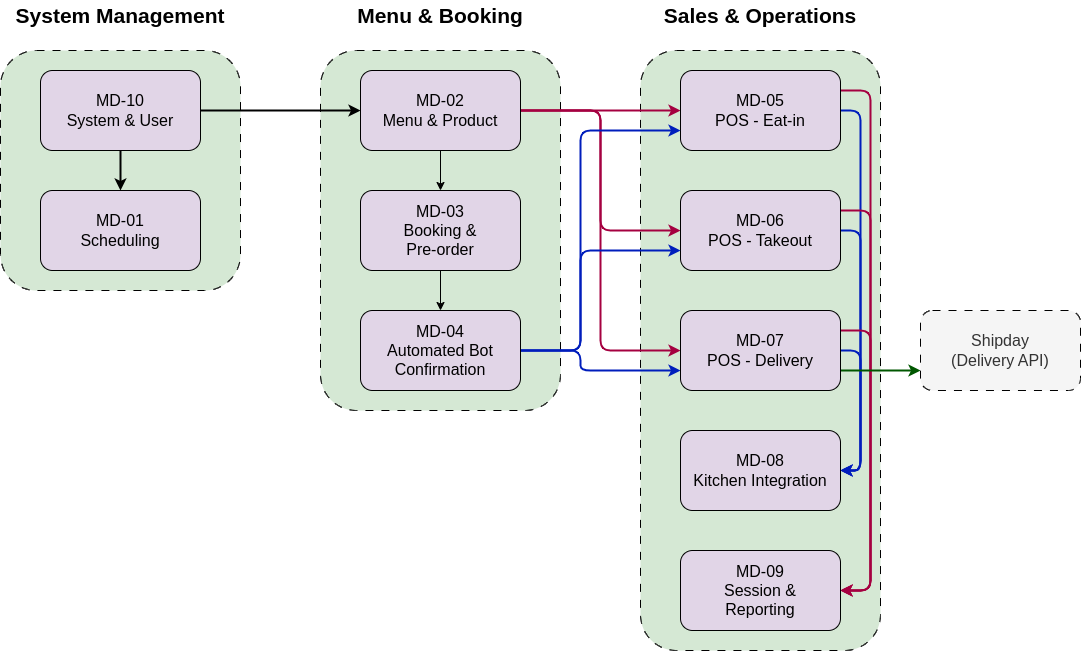
\includegraphics[width=10cm]{Images/kthtm.png}
    \vspace{0.5cm}
    \caption{Sơ đồ luồng kiến trúc hệ thống theo module chức năng}
    \label{fig:my_label}
\end{figure}

Sơ đồ luồng kiến trúc hệ thống được thiết kế để minh họa mối quan hệ và luồng dữ liệu giữa các module chức năng trong hệ thống quản lý nhà hàng. Các module được chia thành ba nhóm chính: Quản lý hệ thống (System Management), Quản lý thực thực đơn và đặt chỗ (Menu & Booking), và Bán hàng & Vận hành (Sales & Operations). Mỗi module, từ quản lý lịch làm việc (MD-01) đến báo cáo doanh thu (MD-09), được kết nối với nhau thông qua các luồng dữ liệu rõ ràng, hỗ trợ các chức năng như đặt chỗ, bán hàng tại chỗ, giao hàng và tích hợp với hệ thống bên ngoài như Shipday. Sơ đồ sử dụng bố cục lưới với các đường dẫn cong để đảm bảo tính trực quan và dễ theo dõi.

% Hệ thống bao gồm các thành phần như sau:
% \begin{enumerate}
%     \item \textbf{Frontend}
%     \begin{itemize}
%         \item Được phát triển bằng ReactJS.
%         \item Giao tiếp với backend thông qua RESTful API.
%         \item Cung cấp giao diện người dùng trực quan, tối ưu trải nghiệm (UX/UI), hỗ trợ responsive trên nhiều thiết bị.
%         \item Xử lý logic hiển thị, xác thực người dùng và tương tác với API.
%     \end{itemize}
%     \item \textbf{Backend}
%     \begin{itemize}
%         \item Được xây dựng bằng Spring Boot, theo mô hình Modular Monolithic và tổ chức theo nguyên tắc Domain-Driven Design (DDD).
%         \item Cung cấp API RESTful để frontend và các hệ thống khác có thể truy cập dữ liệu.
%         \item Xử lý các nghiệp vụ cốt lõi của hệ thống, bao gồm quản lý đặt bàn, thực đơn, đơn hàng, thanh toán, báo cáo, v.v.
%         \item Sử dụng Spring Security để xác thực và phân quyền người dùng.
%         \item Hỗ trợ caching bằng Redis để tăng hiệu suất truy vấn dữ liệu.
%     \end{itemize}
%     \item \textbf{Cơ sở dữ liệu}
%     \begin{itemize}
%         \item Sử dụng PostgreSQL làm hệ quản trị cơ sở dữ liệu chính.
%         \item Được thiết kế theo nguyên tắc CQRS (Command Query Responsibility Segregation) nhằm tối ưu hóa hiệu suất đọc/ghi.
%     \end{itemize}
%     \item \textbf{Third-party Integrations}
%     \begin{itemize}
%         \item Hỗ trợ kết nối với các cổng thanh toán như VNPay, Momo, Stripe để xử lý giao dịch.
%         \item Tích hợp với các dịch vụ bên ngoài như SMS, Email (SendGrid, Twilio), CRM, POS để mở rộng chức năng của hệ thống.
%     \end{itemize}


% \subsection{Kiến trúc phần mềm}
% % \subsubsection{Mô hình MVC \cite{MVC}}
% MVC là viết tắt của khái niệm "Model-View-Controller", một trong những mô hình thiết kế phần mềm phổ biến nhất.\\

% MVC tách biệt dữ liệu, giao diện người dùng và logic xử lý thành ba thành phần riêng biệt nhưng vẫn được kết nối chặt chẽ với nhau.

% \begin{itemize}
%     \item Model (M): Đại diện cho dữ liệu và logic xử lý các nghiệp vụ của ứng dụng.
%     \item View (V): Quản lý giao diện và hiển thị dữ liệu ra cho người dùng.
%     \item Controller (C): Làm điều phối và điều hướng tương tác giữa Model và View. Nó nhận yêu cầu từ View, thực hiện xử lý trên Model và trả kết quả về cho View hiển thị.
% \end{itemize}

% MVC giúp tách biệt các thành phần của ứng dụng, tăng tính bảo trì và khả năng mở rộng trong tương lai.\\

% \begin{figure}[H]
%     \centering
%     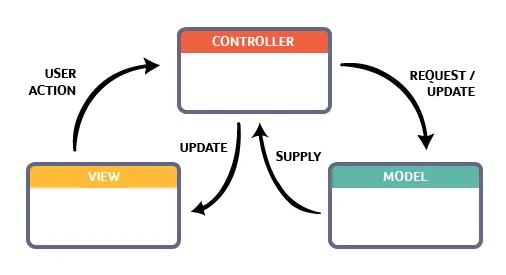
\includegraphics[width=10cm]{Images/ezgif-4-c53032b3fd.png}
%     \vspace{0.5cm}
%     \caption{MVC là gì?}
%     \label{fig:my_label}
% \end{figure}

% Mô hình MVC (MVC pattern) thường được dùng để phát triển giao diện người dùng. Nó cung cấp các thành phần cơ bản để thiết kế một chương trình cho máy tính hoặc điện thoại di động, cũng như là các ứng dụng web.

% \subsubsection{Các thành phần của MVC}
% Mô hình MVC gồm 3 loại chính là thành phần bên trong không thể thiếu khi áp dụng mô hình này:
% \begin{figure}[H]
%     \centering
%     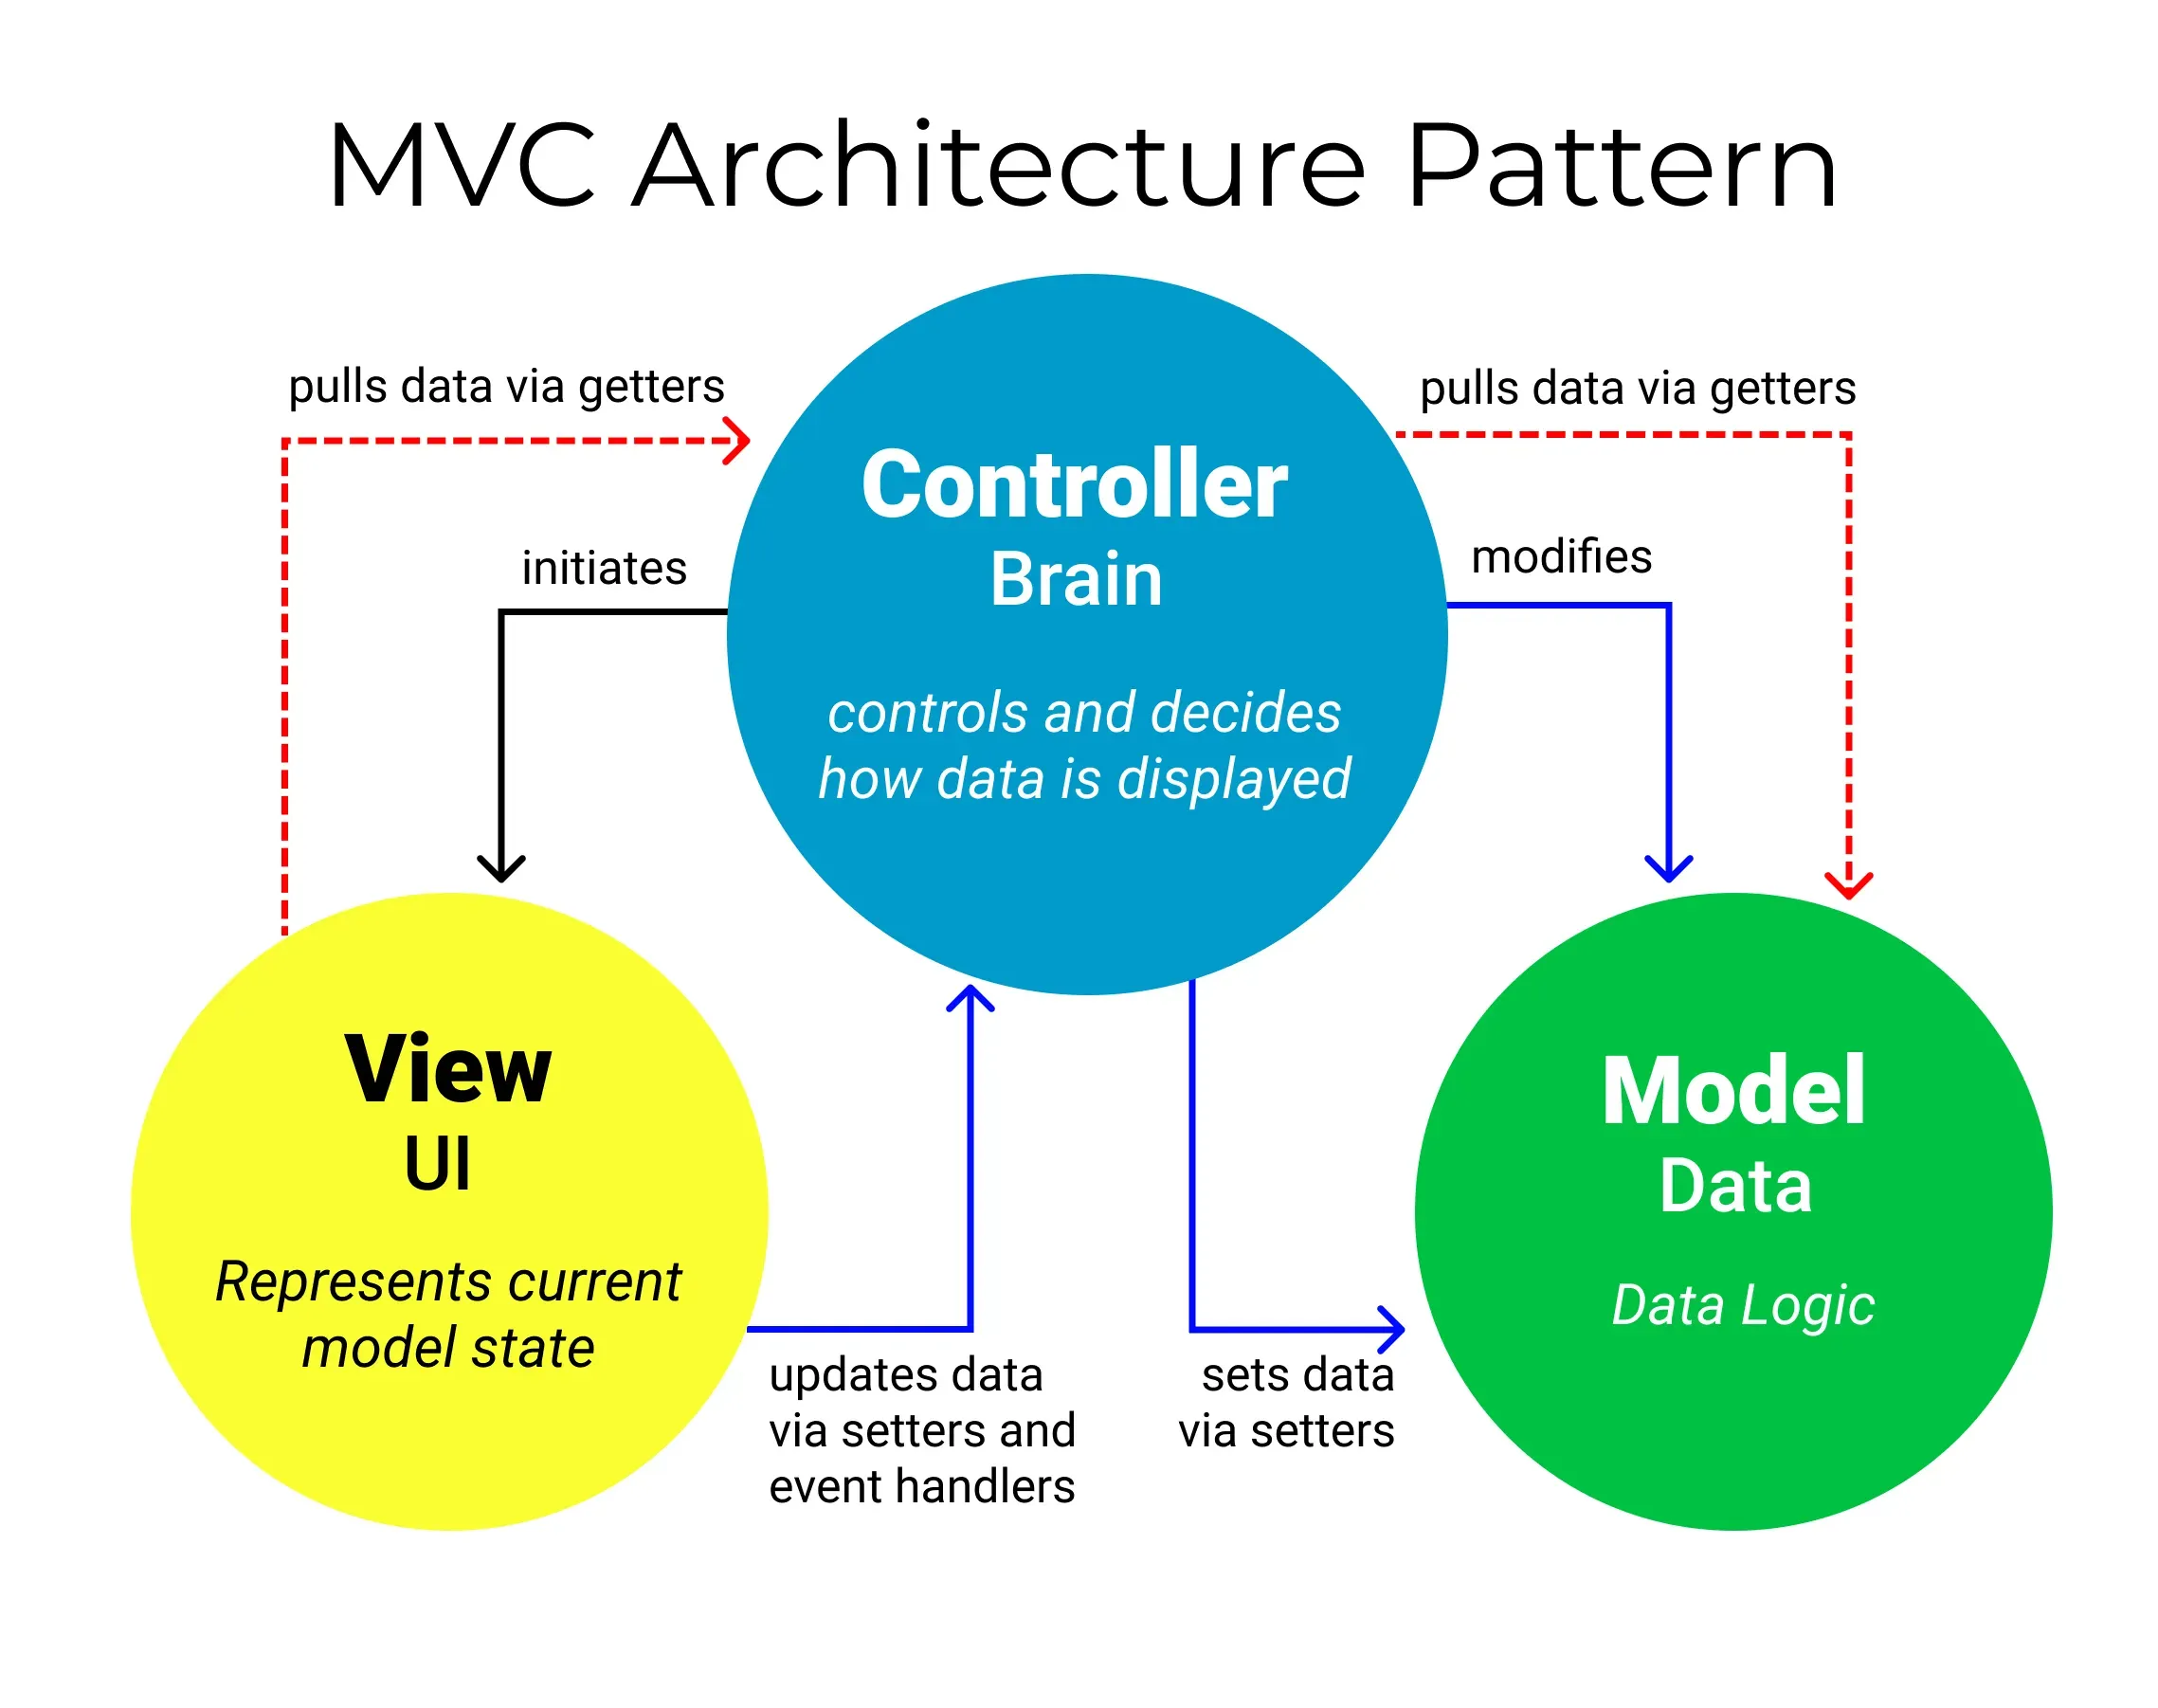
\includegraphics[width=10cm]{Images/cacthanhphanmvc.png}
%     \vspace{0.5cm}
%     \caption{Thành phần của MVC}
%     \label{fig:my_label}
% \end{figure}

% \begin{itemize}
%     \item Model: Là bộ phận có chức năng lưu trữ toàn bộ dữ liệu của ứng dụng và là cầu nối giữa 2 thành phần bên dưới là View và Controller. Một model là dữ liệu được sử dụng bởi chương trình. Đây có thể là cơ sở dữ liệu, hoặc file XML bình thường hay một đối tượng đơn giản. Chẳng hạn như biểu tượng hay là một nhân vật trong game.
%     \item View: Đây là phần giao diện (theme) dành cho người sử dụng. View là phương tiện hiển thị các đối tượng trong một ứng dụng. Chẳng hạn như hiển thị một cửa sổ, nút hay văn bản trong một cửa sổ khác. Nó bao gồm bất cứ thứ gì mà người dùng có thể nhìn thấy được.
%     \item Controller: Là bộ phận có nhiệm vụ xử lý các yêu cầu người dùng đưa đến thông qua View. Một controller bao gồm cả Model lẫn View. Nó nhận input và thực hiện các update tương ứng.
% \end{itemize}

% \subsubsection{Luồng xử lý trong MVC}
% Luồng xử lý trong của mô hình MVC, bạn có thể hình dung cụ thể và chi tiết qua từng bước dưới đây:
% \begin{itemize}
%     \item Khi một yêu cầu của từ máy khách (Client) gửi đến Server. Thì bị Controller trong MVC chặn lại để xem đó là URL request hay sự kiện.
%     \item Sau đó, Controller xử lý input của user rồi giao tiếp với Model trong MVC.
%     \item Model chuẩn bị data và gửi lại cho Controller.
%     \item Cuối cùng, khi xử lý xong yêu cầu thì Controller gửi dữ liệu trở lại View và hiển thị cho người dùng trên trình duyệt.
% \end{itemize}
% \begin{figure}[H]
%     \centering
%     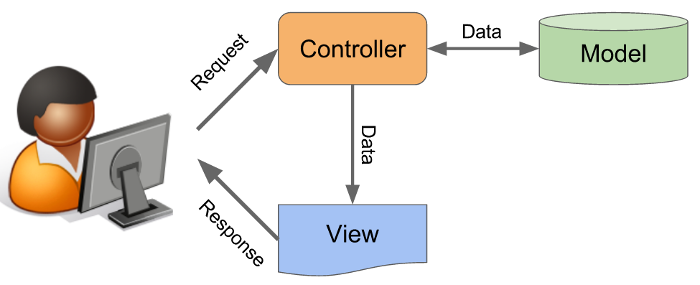
\includegraphics[width=10cm]{Images/luongmvc.png}
%     \vspace{0.5cm}
%     \caption{View và Model sẽ được xử lý bởi Controller}
%     \label{fig:my_label}
% \end{figure}

% Ở đây, View không giao tiếp trực tiếp với Model. Sự tương tác giữa View và Model sẽ chỉ được xử lý bởi Controller.
\subsubsection{Ưu và nhược điểm của MVC}
\textbf{Ưu điểm mô hình MVC}
\begin{itemize}
    \item Đầu tiên, nhắc tới ưu điểm mô hình MVC thì đó là băng thông (Bandwidth) nhẹ vì không sử dụng viewstate nên khá tiết kiệm băng thông. Việc giảm băng thông giúp website hoạt động ổn định hơn.
    \item Kiểm tra đơn giản và dễ dàng, kiểm tra lỗi phần mềm trước khi bàn giao lại cho người dùng.
    \item Một lợi thế chính của MVC là nó tách biệt các phần Model, Controller và View với nhau.
    \item Sử dụng mô hình MVC chức năng Controller có vai trò quan trọng và tối ưu trên các nền tảng ngôn ngữ khác nhau
    \item Ta có thể dễ dàng duy trì ứng dụng vì chúng được tách biệt với nhau.
    \item Có thể chia nhiều developer làm việc cùng một lúc. Công việc của các developer sẽ không ảnh hưởng đến nhau.
    \item Hỗ trợ TTD (test-driven development). Chúng ta có thể tạo một ứng dụng với unit test và viết các won test case.
    \item Phiên bản mới nhất của MVC hỗ trợ trợ thiết kế responsive website mặc định và các mẫu cho mobile. Chúng ta có thể tạo công cụ View của riêng mình với cú pháp đơn giản hơn nhiều so với công cụ truyền thống.
\end{itemize}
\textbf{Nhược điểm mô hình MVC}\\

MVC đa phần phù hợp với công ty chuyên về website hoặc các dự án lớn thì mô hình này phù hợp hơn so với với các dự án nhỏ, lẻ vì khá là cồng kềnh và mất thời gian.

\begin{itemize}
    \item Không thể Preview các trang như ASP.NET.
    \item Khó triển khai.
\end{itemize}
\subsubsection{Lý do sử dụng MVC}
\textbf{Quy trình phát triển nhanh hơn}\\

MVC hỗ trợ phát việc phát triển nhanh chóng và song song. Nếu một mô hình MVC được dùng để phát triển bất kỳ ứng dụng web cụ thể nào, một lập trình viên có thể làm việc trên View và một developer khác có thể làm việc với Controller để tạo logic nghiệp vụ cho ứng dụng web đó.\\

Do đó, ứng dụng mô hình MVC có thể được hoàn thành nhanh hơn ba lần so với các ứng dụng mô hình khác.\\

\textbf{Khả năng cung cấp nhiều chế độ view}\\

Trong mô hình MVC, bạn có thể tạo nhiều View cho chỉ một mô hình. Ngày nay, nhu cầu có thêm nhiều cách mới để truy cập ứng dụng và đang ngày càng tăng. Do đó, việc sử dụng MVC để phát triển chắc chắn là một giải pháp tuyệt vời.\\

Hơn nữa, với phương pháp này, việc nhân bản code rất hạn chế. Vì nó tách biệt dữ liệu và logic nghiệp vụ khỏi màn hình.\\

\textbf{Các sửa đổi không ảnh hưởng đến toàn bộ mô hình}\\

Đối với bất kỳ ứng dụng web nào, người dùng có xu hướng thay đổi thường xuyên. Bạn có thể quan sát thông qua những thay đổi thường xuyên về màu sắc, font chữ, bố cục màn hình. Hay là thêm hỗ trợ thiết bị mới cho điện thoại hay máy tính bảng…\\

Việc thêm một kiểu view mới trong MVC rất đơn giản. Vì phần Model không phụ thuộc vào phần View. Do đó, bất kỳ thay đổi nào trong Model sẽ không ảnh hưởng đến toàn bộ kiến trúc.\\

\textbf{MVC Model trả về dữ liệu mà không cần định dạng}\\

MVC pattern có thể trả về dữ liệu mà không cần áp dụng bất kỳ định dạng nào. Do đó, các thành phần giống nhau có thể được sử dụng với bất kỳ giao diện nào.\\

Ví dụ: tất cả loại dữ liệu đều có thể được định dạng bằng HTML. Ngoài ra, nó cũng có thể được định dạng bằng Macromedia Flash hay Dream Viewer.\\



\subsection{Thiết kế Sitemap}

\begin{figure}[H]
    \centering
    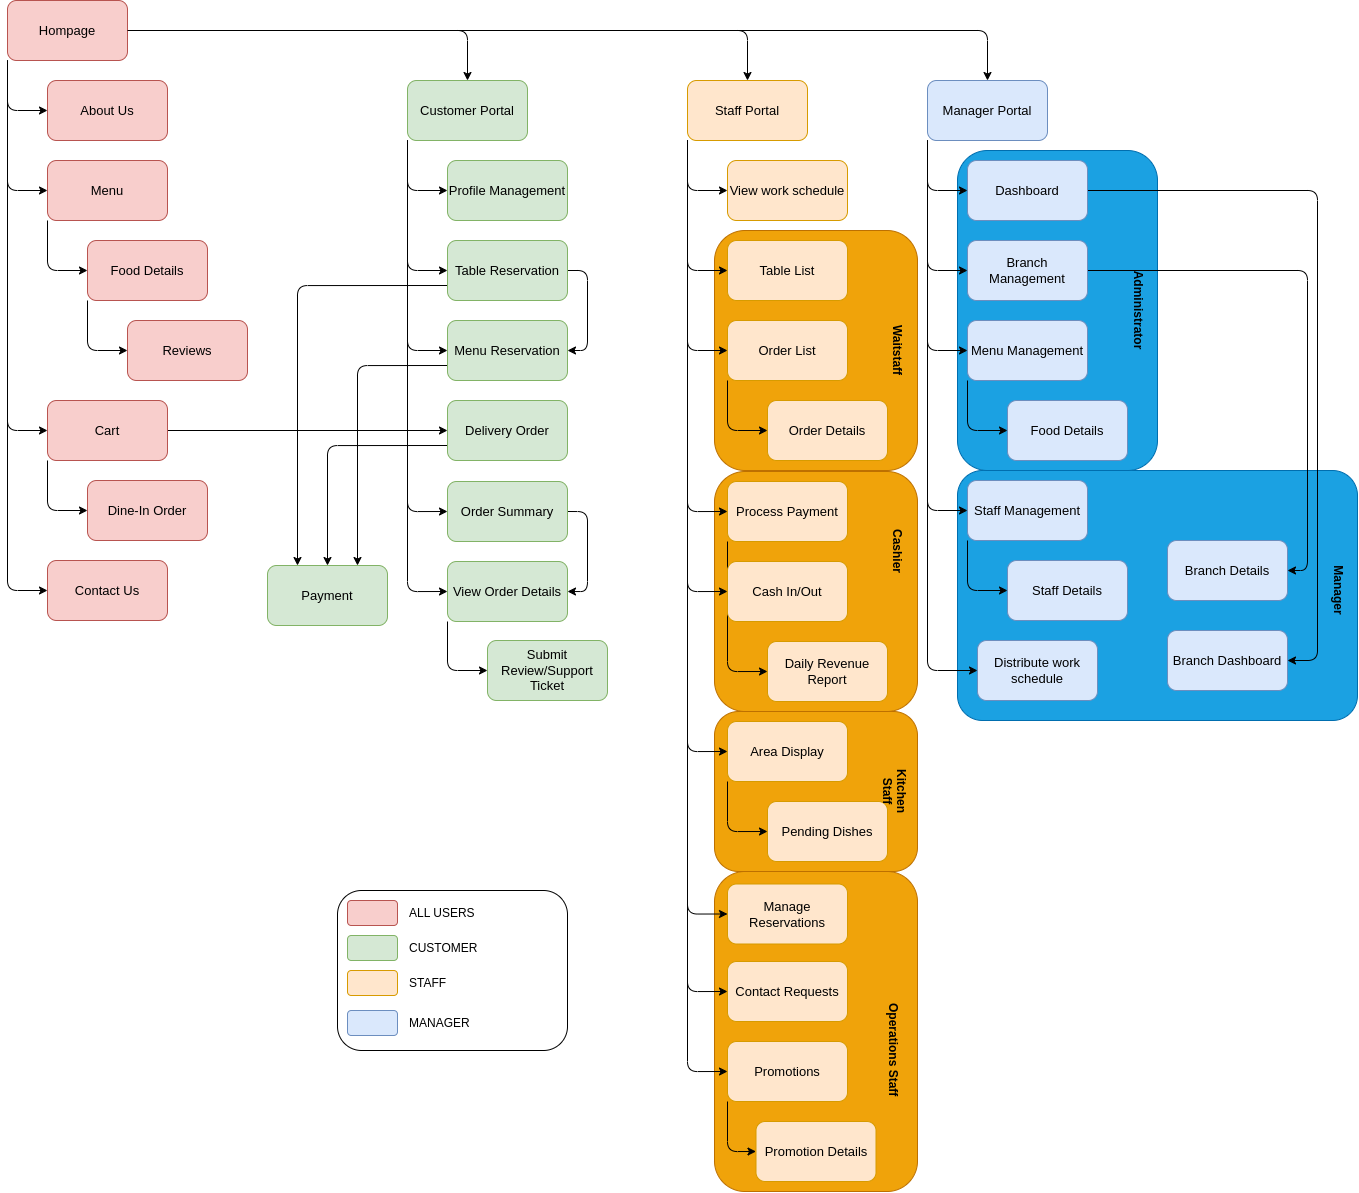
\includegraphics[width=\linewidth]{Images/sitemap.png}
    \vspace{0.5cm}
    \caption{Sitemap của hệ thống}
    \label{fig:my_label}
\end{figure}

Sitemap này mô tả cấu trúc và các tính năng chính của Hệ thống quản lý đặt món cho nhà hàng, nêu chi tiết các chức năng và mô-đun cốt lõi của nó.

\begin{enumerate}
    \item \textbf{Tất cả người dùng}
        \begin{itemize}
            \item \textit{Homepage}: Trang chính của ứng dụng, hiển thị thông tin giới thiệu về nhà hàng, các danh mục chính (Menu, Đặt hàng, Liên hệ), và nút đăng nhập/đăng ký để chuyển đến các cổng phù hợp với vai trò người dùng.
            \item \textit{About Us (Giới thiệu)}: Cung cấp thông tin về nhà hàng, bao gồm lịch sử, giá trị cốt lõi, đội ngũ, và các chi nhánh.
            \item \textit{Menu}: Hiển thị danh sách các món ăn và khuyến mãi hiện có, phân loại theo loại (đồ ăn, đồ uống, món tráng miệng), cho phép người dùng xem chi tiết món ăn và thêm vào giỏ hàng.
            \item \textit{Food Details (Chi tiết món ăn)}: Food Details (Chi tiết món ăn): Hiển thị thông tin chi tiết về một món ăn cụ thể (tên, giá, mô tả, hình ảnh, thành phần, đánh giá), cho phép thêm vào giỏ hàng hoặc quay lại danh sách menu.
            \item \textit{Cart (Giỏ hàng)}: Hiển thị danh sách món ăn đã chọn, cho phép chỉnh sửa số lượng và ghi chú, xóa món, và chọn phương thức đặt hàng (Dine-In Order hoặc Delivery Order).
            \item \textit{Dine-In Order (Đặt món tại quán)}: Cho phép người dùng xác nhận đơn hàng để ăn tại quán, cho phép chuyển sang trang thanh toán khi hoàn thành bữa ăn.
            \item \textit{Payment (Thanh toán)}: Xử lý thanh toán cho đơn hàng tại quán, hỗ trợ các phương thức thanh toán (tiền mặt, thẻ, QR code), và hiển thị xác nhận sau khi thanh toán thành công.
            \item \textit{Contact Us (Liên hệ)}: Cung cấp thông tin liên hệ (số điện thoại, email, địa chỉ), và biểu mẫu để khách hàng gửi câu hỏi hoặc phản hồi.
        \end{itemize}
    \item \textbf{Khách hàng đã có tài khoản}
        \begin{itemize}
            \item \textit{Profile Management (Quản lý thông tin cá nhân)}: Cho phép khách hàng xem và chỉnh sửa thông tin cá nhân (tên, số điện thoại, email, địa chỉ), quản lý tài khoản và mật khẩu.
            \item \textit{Table Reservation (Đặt bàn)}: Cho phép khách hàng chọn thời gian, số lượng người, xem sơ đồ và đặt bàn tại nhà hàng, với xác nhận qua email hoặc tin nhắn. Nếu đang có yêu cầu đặt bàn thì cũng sẽ hiển thị và hủy ở đây.
            \item \textit{Delivery Order (Đặt món giao về)}: Cho phép người dùng chọn giao hàng, nhập thông tin giao hàng (địa chỉ, số điện thoại), và chuyển sang trang thanh toán.
            \item \textit{Order Summary (Tóm tắt đơn hàng)}: Hiển thị tất cả đơn hàng (món ăn, số lượng, tổng tiền, thông tin giao hàng), cho phép chuyển qua trang xem chi tiết.
            \item \textit{View Order Details (Xem chi tiết đơn hàng)}: Hiển thị trạng thái và thông tin chi tiết của một đơn hàng đã đặt (thời gian, địa chỉ, tình trạng giao hàng), cho phép khách hàng theo dõi. Nếu đơn hàng đã thành công, có thể chuyển đến trang gửi đánh giá.
            \item \textit{Submit Review (Gửi đánh giá)}: Cho phép người dùng viết đánh giá hoặc xếp hạng cho món ăn hoặc dịch vụ sau khi hoàn tất đơn hàng, gửi lên hệ thống.
        \end{itemize}
    \item \textbf{Nhân viên}
    
        \textbf{\textit{Tất cả nhân viên}}
        \begin{itemize}
            \item \textit{View word schedule (Xem lịch làm)}: Hiển thị lịch làm việc được xếp.
        \end{itemize}
        \textbf{\textit{Nhân viên Phục vụ}}
        \begin{itemize}
            \item \textit{Table List (Danh sách bàn)}: Hiển thị trạng thái các bàn (trống, đang sử dụng, đặt trước), cho phép nhân viên phục vụ cập nhật hoặc quản lý.
            \item \textit{Order List (Danh sách đơn hàng)}: Hiển thị danh sách các đơn hàng đang chờ xử lý, cho phép nhân viên chọn đơn để xem chi tiết hoặc chuyển sang bếp.
            \item \textit{Order Details (Chi tiết đơn hàng)}: Hiển thị thông tin chi tiết của một đơn hàng (món ăn, số lượng, ghi chú), cho phép nhân viên xác nhận hoặc cập nhật trạng thái.
        \end{itemize}
            
        \textit{\textbf{Nhân viên Thu ngân}}
        \begin{itemize}
            \item \textit{Process Payment (Xử lý thanh toán)}: Cho phép nhân viên thu ngân nhập thông tin thanh toán, xử lý các phương thức (tiền mặt, thẻ), và xuất hóa đơn.
            \item \textit{Cash In/Out}: Thêm thông tin vào dòng tiền bên ngoài.
            \item \textit{Daily Revenue Report (Báo cáo doanh thu hàng ngày)}: Hiển thị tổng doanh thu, số lượng đơn hàng, và các thống kê khác trong ngày, hỗ trợ nhân viên thu ngân theo dõi.
        \end{itemize}
            
        \textit{\textbf{Nhân viên Bếp}}
        \begin{itemize}
            \item \textit{Area Display (Các khu vực bếp): Hiển thị danh sách các khu vực bếp tương ứng với các món ăn được chỉ định sẵn.}
            \item \textit{Pending Dishes (Món ăn đang chờ)}: Hiển thị danh sách món ăn cần chuẩn bị, cho phép nhân viên bếp theo dõi và cập nhật trạng thái hoàn thành.
        \end{itemize}
            
        \textit{\textbf{Nhân viên Vận hành}}
        \begin{itemize}
            \item \textit{Manage Reservations (Quản lý đặt bàn)}: Cho phép nhân viên xem, chỉnh sửa, hoặc hủy đặt bàn (bao gồm hủy khi khách đến trễ quá), cập nhật trạng thái bàn.
            \item \textit{Contact Requests (Yêu cầu liên hệ)}: Hiển thị danh sách yêu cầu hỗ trợ từ khách hàng, cho phép nhân viên hỗ trợ trả lời hoặc chuyển tiếp.
            \item \textit{Promotions (Khuyến mãi)}: Hiển thị danh sách các chương trình khuyến mãi hiện tại, cho phép quản lý tạo mới hoặc chỉnh sửa.
            \item \textit{Promotion Details (Chi tiết khuyến mãi)}: Hiển thị thông tin chi tiết của từng chương trình khuyến mãi (thời gian, điều kiện, ưu đãi), cho phép chỉnh sửa hoặc xóa. Thống kê số liệu về chương trình khuyến mãi
        \end{itemize}
    \item \textbf{Quản lý}
        \begin{itemize}
            \item \textit{Staff Management (Quản lý nhân viên)}: Cho phép quản lý thêm, chỉnh sửa, hoặc xóa thông tin nhân viên (tên, vai trò, lịch làm việc).
            \item \textit{Staff Details (Chi tiết nhân viên)}: Hiển thị thông tin chi tiết của từng nhân viên (hồ sơ, lịch sử làm việc, hiệu suất), cho phép chỉnh sửa.
            \item \textit{Branch Details (Chi tiết chi nhánh)}: Hiển thị thông tin chi tiết của chi nhánh, cho phép chỉnh sửa sơ đồ nhà hàng.
            \item \textit{Branch Dashboard (Bảng điều khiển chi nhánh)}: Hiển thị thông tin cụ thể của từng chi nhánh (doanh thu, đơn hàng, nhân viên), hỗ trợ quản lý theo dõi.
            \item \textit{Distribute work schedule (Xếp lịch làm)}: Cho phép lập lịch trực qua, thêm ghi chú công việc cho nhân viên.
        \end{itemize}
        
        \textit{\textbf{Dành cho quản trị viên}}
        \begin{itemize}
            \item \textit{Dashboard (Bảng điều khiển)}: Hiển thị tổng quan về hoạt động nhà hàng (doanh thu, số đơn hàng, trạng thái nhân viên), với các biểu đồ và số liệu chính.
            \item \textit{Branch Management (Quản lý chi nhánh)}: Cho phép quản lý thêm, chỉnh sửa, hoặc xóa thông tin chi nhánh (địa chỉ, số điện thoại, giờ hoạt động).
            \item \textit{Menu Management (Quản lý menu)}: Cho phép quản lý thêm, chỉnh sửa, hoặc xóa món ăn trong menu (tên, giá, hình ảnh, mô tả). Thống kế các thông tin số liệu về món ăn.
            \item \textit{Food Details (Chi tiết món ăn)}: Hiển thị và chỉnh sửa thông tin chi tiết của từng món ăn trong menu (dành cho quản lý).
        \end{itemize}
    
\end{enumerate}

\subsection{Thiết kế Database}
\subsubsection{EERD Database}

Hệ thống cơ sở dữ liệu quản lý một chuỗi nhà hàng, tập trung vào việc quản lý người dùng, nhân viên, khách hàng, đặt bàn, gọi món, hóa đơn thanh toán, chương trình khuyến mãi, phản hồi và hỗ trợ khách hàng. Người dùng (USER) lưu trữ các thông tin như tên đăng nhập, mật khẩu đã mã hóa, họ tên đầy đủ và địa chỉ email. Một người dùng có thể là một nhân viên (STAFF), đảm nhiệm các vai trò như thu ngân (CASHIER), đầu bếp (CHEF), nhân viên phục vụ (WAITER), nhân viên vệ sinh (CLEANING STAFF), nhân viên vận hành (OPERATION STAFF). Người dùng cũng có thể là quản lý (MANAGER) hoặc khách hàng (CUSTOMER). Mỗi nhân viên bắt buộc phải làm việc tại một chi nhánh (BRANCH) cụ thể. Mỗi chi nhánh lưu trữ các thông tin về tên, địa chỉ và số điện thoại liên hệ, đồng thời phải có một bản cấu hình (CONFIGURATION) riêng biệt để thiết lập các chính sách như tiền đặt cọc bàn, tỷ lệ đặt cọc khi đặt món trước, thời gian tự động gọi xác nhận đơn hàng hoặc các thông số kỹ thuật khác. Mỗi chi nhánh có đúng một người quản lý (MANAGER) chịu trách nhiệm vận hành toàn bộ hoạt động tại chi nhánh đó.

Nhân viên làm việc theo ca (SHIFT), mỗi ca ghi nhận giờ bắt đầu, giờ kết thúc, ghi chú đặc biệt nếu có và trạng thái như nháp, xung đột, hoàn thành hoặc đã lên lịch. Nhân viên nhà bếp sẽ được phân công làm việc tại các khu vực bếp (KITCHEN STATION) thuộc từng chi nhánh riêng biệt, mỗi khu vực bếp có tên và mô tả cụ thể. Một chi nhánh phải có ít nhất một khu vực bếp được cấu hình trước khi có thể bắt đầu vận hành.

Nhà hàng bố trí nhiều bàn ăn (TABLE) với các thông tin về số lượng chỗ ngồi và vị trí cụ thể trên bản đồ nhà hàng. Bàn có các trạng thái vận hành như trống, đang sử dụng hoặc chờ làm sạch. Khách hàng có thể thực hiện việc đặt bàn trước (BOOKING TABLE), ghi lại số lượng khách, thời gian ăn, các ghi chú thêm và trạng thái đặt bàn như đã xác nhận, đã hủy hoặc thành công. Khách hàng cũng có thể đặt món trước (BOOKING DISH), ghi nhận các món ăn mong muốn, số lượng từng món, thời gian ăn dự kiến tới ăn và ghi chú riêng cho từng món nếu cần.

Món ăn (DISH) lưu trữ thông tin về tên món, mô tả, kích cỡ phần ăn, giá tiền, thời gian chế biến ước tính và trạng thái hoạt động. Mỗi món ăn được tạo thành từ nhiều nguyên liệu. Ngoài ra, nhà hàng còn xây dựng các combo (COMBO) kết hợp nhiều món ăn với giá ưu đãi để bán cho khách.

Khi khách hàng gọi món hoặc đặt món, hệ thống tạo ra đơn hàng (ORDER) với thông tin loại đơn (ăn tại chỗ, mang đi, giao hàng), trạng thái đơn hàng (thành công, đang thực hiện, đã hủy...), tiền cọc nếu có và tổng giá trị đơn hàng, được tính bằng cách lấy giá từng món ăn hoặc combo (áp dụng giá khuyến mãi nếu có) nhân với số lượng rồi cộng lại. Đối với đơn giao hàng sẽ có thêm thông tin vận chuyển. Mỗi đơn hàng có thể gắn với một hoặc nhiều hóa đơn (INVOICE) trong trường hợp chia nhỏ hóa đơn, ghi lại tổng số tiền thanh toán (sau khi áp dụng voucher nếu có, trừ đi tiền cọc), thuế VAT, thời gian lập hóa đơn và loại hóa đơn (hóa đơn gộp hoặc hóa đơn lẻ). Khách hàng thanh toán qua các phương thức thanh toán (PAYMENT) khác nhau như tiền mặt, ví điện tử hoặc ebanking. Các khoản đặt cọc cho đặt bàn hoặc đặt món cũng được ghi nhận dưới dạng PAYMENT riêng biệt, với số tiền tính theo phần trăm cấu hình tại CONFIGURATION.

Hệ thống quản lý các mã giảm giá (VOUCHER), mỗi voucher có điều kiện áp dụng cụ thể, giới hạn số lần sử dụng, thời gian hiệu lực, lưu lại số phần trăm giảm giá hoặc số tiền giảm giá. Khách hàng có thể lưu trữ các voucher được phát hành để sử dụng về sau nếu voucher còn hiệu lực. Ngoài voucher, nhà hàng còn có các chương trình khuyến mãi (PROMOTION) diễn ra trong các khoảng thời gian xác định, giảm giá trực tiếp trên món ăn.

Khách hàng có thể gửi yêu cầu hỗ trợ (SUPPORT TICKET) với tiêu đề, nội dung cụ thể và trạng thái xử lý như đã xử lý, đang xử lý hoặc đang chờ bổ sung thông tin. Mỗi yêu cầu sẽ được phân công cho nhân viên vận hành để tiếp nhận và xử lý. Khách hàng cũng có thể gửi phản hồi (FEEDBACK) với nội dung giới hạn trong 500 ký tự về dịch vụ hoặc món ăn, gắn liền với từng đơn hàng, và đánh giá chất lượng từ 1 đến 5 sao. Trong trường hợp có sự cố, khách hàng có thể yêu cầu hoàn tiền (REFUND), yêu cầu này gắn liền với hóa đơn (INVOICE) liên quan để nhân viên có thể theo dõi và xử lý.

\begin{landscape}
\begin{figure}[H]
    \centering
    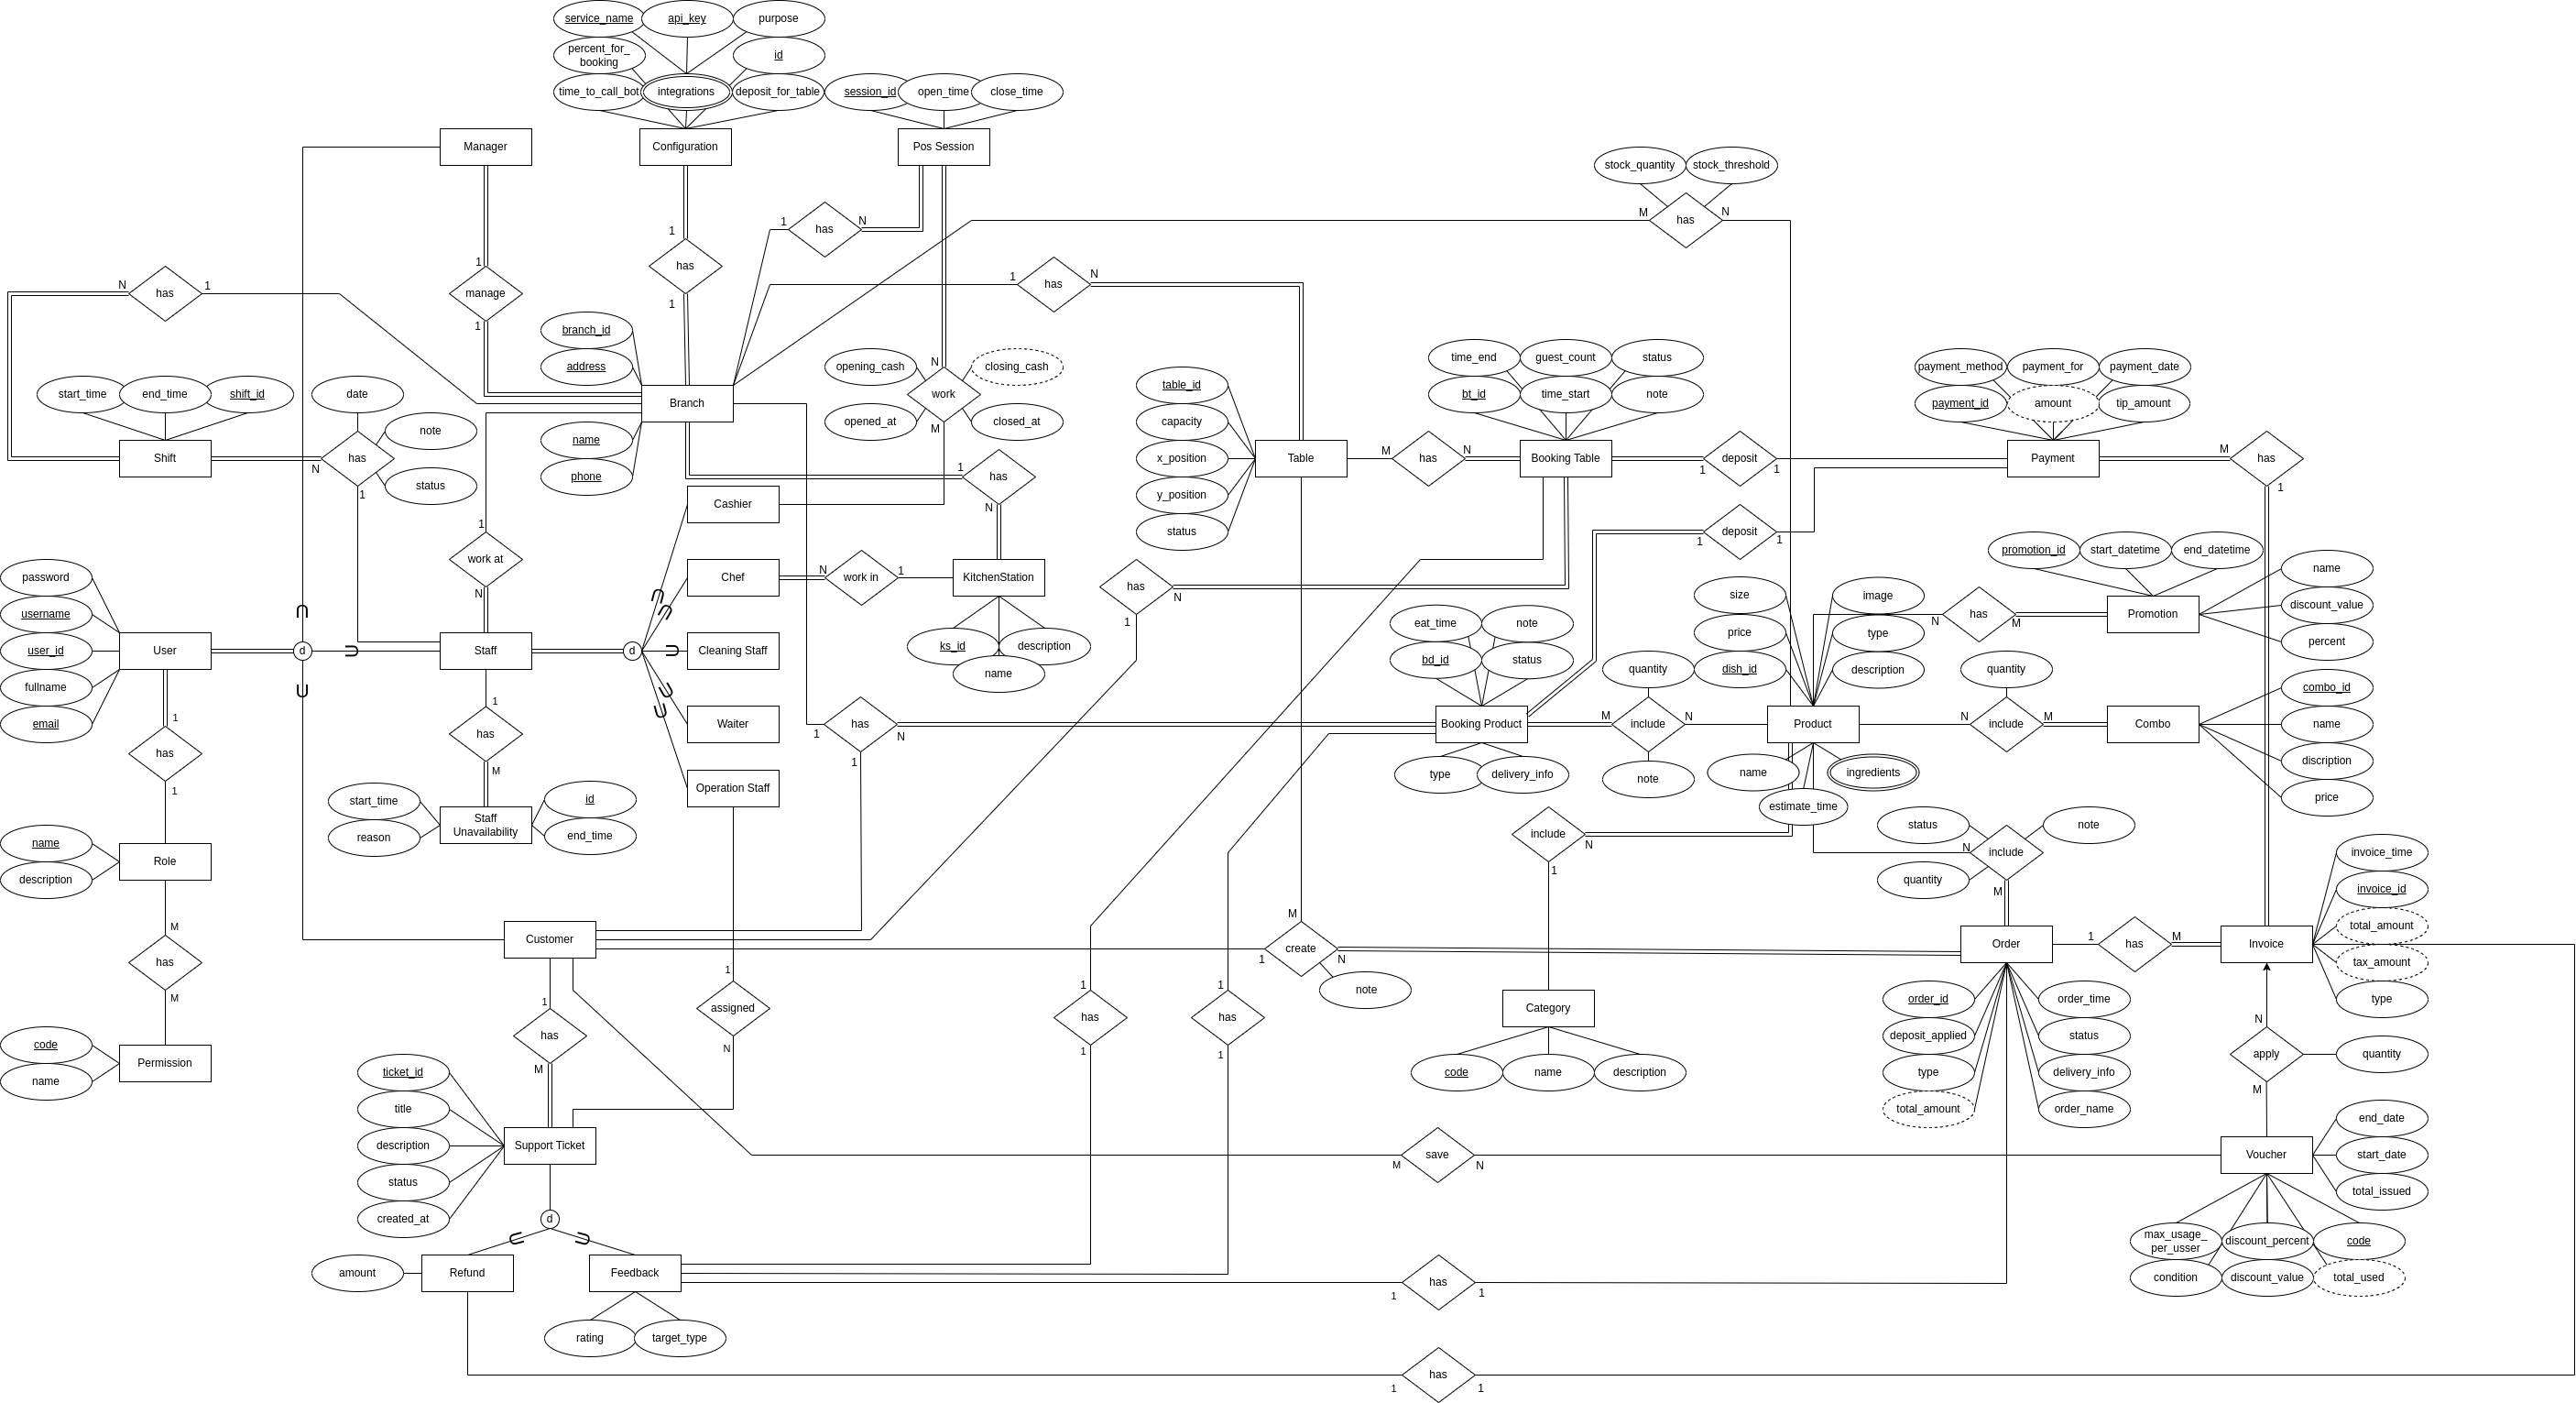
\includegraphics[height=0.85\textheight]{Images/db.png}
    \vspace{0.5cm}
    \caption{EERD của cơ sở dữ liệu}
    \label{fig:my_label}
\end{figure}
\end{landscape}

% \subsubsection{Các ràng buộc}
% \paragraph{Ràng buộc miền trị (Domain Constraints – Attribute Domains):}

% \begin{itemize}
%   \item \textbf{Trạng thái (SHIFT - STAFF)}
%     \begin{itemize}
%         \item \texttt{DRAFT}: Ca làm việc đang trong quá trình tạo, chưa được công bố.
%         \item \texttt{PUBLISHED}: Ca làm việc đã được công bố và có hiệu lực.
%         \item \texttt{CONFLICTED}: Ca làm việc bị xung đột về thời gian hoặc nhân sự.
%     \end{itemize}

%   \item \textbf{Trạng thái (SUPPORT TICKET)}
%     \begin{itemize}
%         \item \texttt{PENDING}: Yêu cầu đang chờ xử lý.
%         \item \texttt{RECEIVED}: Yêu cầu đã được tiếp nhận.
%         \item \texttt{IN\_PROGRESS}: Yêu cầu đang trong quá trình xử lý.
%         \item \texttt{RESOLVED}: Yêu cầu đã được xử lý xong.
%     \end{itemize}

%   \item \textbf{Đánh giá (Feedback)}
%     \begin{itemize}
%         \item Các giá trị từ \texttt{1} đến \texttt{5}, thể hiện mức độ hài lòng của khách hàng.
%     \end{itemize}

%   \item \textbf{Mô tả (Feedback)}
%     \begin{itemize}
%         \item Chuỗi văn bản tối đa \texttt{500} ký tự để khách hàng mô tả chi tiết phản hồi.
%     \end{itemize}

%   \item \textbf{Loại đối tượng phản hồi (Target\_Type)}
%     \begin{itemize}
%         \item \texttt{FEEDBACK\_BOOKING\_TABLE}: Phản hồi về việc đặt bàn.
%         \item \texttt{FEEDBACK\_BOOKING\_PRODUCT}: Phản hồi về món ăn đặt trước.
%         \item \texttt{FEEDBACK\_ORDER}: Phản hồi về đơn hàng đã gọi.
%         \item \texttt{GENERAL\_FEEDBACK}: Phản hồi chung, không phân loại cụ thể.
%     \end{itemize}

%   \item \textbf{Trạng thái (TABLE)}
%     \begin{itemize}
%         \item \texttt{AVAILABLE}: Bàn sẵn sàng sử dụng.
%         \item \texttt{OCCUPIED}: Bàn đang có khách.
%         \item \texttt{NEEDS\_CLEANING}: Bàn cần được dọn dẹp.
%     \end{itemize}

%   \item \textbf{Loại hình (BOOKING PRODUCT và ORDER)}
%     \begin{itemize}
%         \item \texttt{DINE\_IN}: Dùng món tại nhà hàng.
%         \item \texttt{TAKE\_AWAY}: Mua mang về.
%         \item \texttt{DELIVERY}: Giao hàng tận nơi.
%     \end{itemize}

%   \item \textbf{Trạng thái (BOOKING TABLE và BOOKING PRODUCT)}
%     \begin{itemize}
%         \item \texttt{BOOKED}: Đã đặt.
%         \item \texttt{DEPOSIT\_PAID}: Đã thanh toán tiền cọc.
%         \item \texttt{CANCELLED}: Đã hủy.
%         \item \texttt{COMPLETED}: Đã hoàn tất dịch vụ.
%     \end{itemize}

%   \item \textbf{Loại sản phẩm (PRODUCT)}
%     \begin{itemize}
%         \item \texttt{CONSUMABLE}: Món ăn đếm được, ví dụ: chai rượu, hộp bánh.
%         \item \texttt{STOCKABLE}: Món ăn không đếm đơn vị, ví dụ: tô cơm, nồi canh.
%         \item \texttt{SERVICE}: Các dịch vụ khác.
%     \end{itemize}

%   \item \textbf{Trạng thái (ORDER)}
%     \begin{itemize}
%         \item \texttt{PLACED}: Đơn hàng đã được tạo.
%         \item \texttt{PREPARING}: Đơn hàng đang được chuẩn bị.
%         \item \texttt{COMPLETED}: Đơn hàng đã hoàn tất.
%         \item \texttt{CANCELLED}: Đơn hàng đã bị hủy.
%     \end{itemize}

%   \item \textbf{Trạng thái (PRODUCT-ORDER)}
%     \begin{itemize}
%         \item \texttt{PENDING}: Món chờ chuẩn bị.
%         \item \texttt{PREPARING}: Đang được chuẩn bị.
%         \item \texttt{COMPLETED}: Đã chuẩn bị xong.
%         \item \texttt{SERVED}: Đã phục vụ cho khách.
%         \item \texttt{CANCELLED}: Đã hủy.
%     \end{itemize}

%   \item \textbf{Loại hóa đơn (INVOICE)}
%     \begin{itemize}
%         \item \texttt{NORMAL}: Hóa đơn bình thường cho một đơn hàng.
%         \item \texttt{MERGED}: Hóa đơn gộp từ nhiều đơn hàng.
%         \item \texttt{SPLIT}: Hóa đơn chia nhỏ từ một đơn hàng.
%     \end{itemize}

%   \item \textbf{Mục đích thanh toán (Payment\_For)}
%     \begin{itemize}
%         \item \texttt{DEPOSIT\_BOOKING\_TABLE}: Tiền cọc cho việc đặt bàn.
%         \item \texttt{DEPOSIT\_BOOKING\_PRODUCT}: Tiền cọc cho đặt món trước.
%         \item \texttt{INVOICE\_PAYMENT}: Thanh toán cho hóa đơn.
%     \end{itemize}

%   \item \textbf{Phương thức thanh toán (Payment\_Method)}
%     \begin{itemize}
%         \item \texttt{CASH}: Thanh toán bằng tiền mặt.
%         \item \texttt{CARD}: Thanh toán qua thẻ (ghi nợ hoặc tín dụng).
%         \item \texttt{EBANKING}: Thanh toán qua ngân hàng điện tử.
%         \item \texttt{E\_WALLET}: Thanh toán qua ví điện tử (Momo, ZaloPay, v.v.)
%     \end{itemize}
% \end{itemize}

% \paragraph{Ràng buộc tham chiếu/thời gian (Referential/Temporal Constraints):}
% \begin{itemize}
%   \item \textbf{POS Session}: Thời gian phiên làm việc phải trùng với thời gian của một ca làm việc (shift) tại cùng chi nhánh (branch).
%   \item \textbf{Thời gian bắt đầu/kết thúc}: Mọi thời điểm kết thúc (end\_time) phải luôn lớn hơn thời điểm bắt đầu (start\_time).
%   \item \textbf{Ràng buộc khuyến mãi (Promotion)}: Trong cùng một khoảng thời gian, mỗi sản phẩm (product) chỉ được áp dụng tối đa một khuyến mãi duy nhất.
% \end{itemize}

% \paragraph{Thuộc tính dẫn xuất (Derived Attributes):}
% \begin{itemize}
%   \item \textbf{closing\_cash (POS Session - Thu ngân)}: Tổng doanh thu trong phiên, sau khi đã trừ các khoản khuyến mãi và voucher.

%   \item \textbf{total\_amount (Order)}: Tính bằng tổng \textit{(đơn giá món ăn hoặc giá khuyến mãi nếu có) \texttimes số lượng} cộng với \textit{giá trị combo \texttimes số lượng}, sau đó trừ đi khoản đặt cọc (nếu có).

%   \item \textbf{total\_amount (Invoice)}: Tính từ \textit{total\_amount} của đơn hàng, áp dụng voucher tương ứng. Nếu là hóa đơn gộp thì cộng tổng nhiều đơn hàng. Nếu là hóa đơn chia thì lấy phần giá trị được chia.

%   \item \textbf{tax\_amount (Invoice)}: Bằng \textit{total\_amount \texttimes thuế suất} do chi nhánh cấu hình.

%   \item \textbf{total\_used (Voucher)}: Tổng số lần voucher đã được sử dụng trong các hóa đơn.

%   \item \textbf{amount (Payment)}:
%     \begin{itemize}
%         \item \texttt{DEPOSIT\_BOOKING\_TABLE}: Số bàn \texttimes giá trị đặt cọc của chi nhánh.
%         \item \texttt{DEPOSIT\_BOOKING\_PRODUCT}: Tổng giá trị món ăn \texttimes phần trăm đặt cọc theo chi nhánh.
%         \item \texttt{INVOICE\_PAYMENT}: Bằng tổng \textit{total\_amount + tax\_amount} của hóa đơn.
%     \end{itemize}
% \end{itemize}

\subsubsection{Thiết kế luận lý}

Thiết kế luận lý thể hiện cấu trúc cơ sở dữ liệu dưới dạng các bảng quan hệ, bao gồm tên bảng, các thuộc tính, khóa chính, khóa ngoại và mối quan hệ giữa chúng. Trong phần này, chúng tôi trình bày \textbf{một số bảng quan trọng tiêu biểu} trong hệ thống quản lý đặt món cho chuỗi nhà hàng, tập trung vào những bảng cốt lõi phục vụ chức năng đặt món, đặt bàn và xử lý đơn hàng.
    
\begin{longtable}{|l|p{6cm}|l|l|}
\hline
\textbf{Tên thuộc tính} & \textbf{Mô tả} & \textbf{Loại khóa} & \textbf{Bảng liên quan} \\
\hline
\endfirsthead

% \multicolumn{4}{c}%
% {{\bfseries \tablename\ \thetable{} -- tiếp theo}} \\
\hline
\textbf{Tên thuộc tính} & \textbf{Mô tả} & \textbf{Loại khóa} & \textbf{Bảng liên quan} \\
\hline
\endhead

\hline \multicolumn{4}{|r|}{{Còn tiếp ...}} \\
\hline
\endfoot

\hline
\endlastfoot

\multicolumn{4}{|c|}{\textbf{Bảng branch}} \\
\hline
id & Định danh chi nhánh & PK & - \\
\hline

\multicolumn{4}{|c|}{\textbf{Bảng category}} \\
\hline
id & Định danh danh mục & PK & - \\
\hline

\multicolumn{4}{|c|}{\textbf{Bảng promotion}} \\
\hline
id & Định danh khuyến mãi & PK & - \\
\hline

\multicolumn{4}{|c|}{\textbf{Bảng combo}} \\
\hline
id & Định danh combo & PK & - \\
\hline

\multicolumn{4}{|c|}{\textbf{Bảng product}} \\
\hline
id & Định danh sản phẩm & PK & - \\
category\_id & Danh mục sản phẩm & FK & category \\
\hline

\multicolumn{4}{|c|}{\textbf{Bảng product\_promotion}} \\
\hline
id & Định danh liên kết giữa khuyến mãi và sản phẩm & PK & - \\
product\_id & Liên kết tới sản phẩm & FK & product \\
promotion\_id & Liên kết tới khuyến mãi & FK & promotion \\
\hline

\multicolumn{4}{|c|}{\textbf{Bảng combo\_product}} \\
\hline
id & Định danh liên kết giữa combo và sản phẩm & PK & - \\
product\_id & Liên kết tới sản phẩm & FK & product \\
combo\_id & Liên kết tới conbo & FK & combo \\
\hline

\multicolumn{4}{|c|}{\textbf{Bảng orders}} \\
\hline
id & Định danh đơn hàng & PK & - \\
customer\_id & Người đặt hàng & FK & user \\
\hline

\multicolumn{4}{|c|}{\textbf{Bảng order\_product}} \\
\hline
id & Định danh dòng món trong đơn hàng & PK & - \\
order\_id & Liên kết tới đơn hàng & FK & orders \\
product\_id & Liên kết tới sản phẩm & FK & product \\
\hline

\multicolumn{4}{|c|}{\textbf{Bảng restaurant\_table}} \\
\hline
id & Định danh bàn ăn & PK & - \\
branch\_id & Thuộc chi nhánh & FK & branch \\
\hline

\multicolumn{4}{|c|}{\textbf{Bảng order\_table}} \\
\hline
id & Định danh liên kết giữa bàn và đơn hàng & PK & - \\
order\_id & Liên kết tới đơn hàng & FK & orders \\
table\_id & Liên kết tới bàn ăn & FK & restaurant\_table \\
\hline

\multicolumn{4}{|c|}{\textbf{Bảng booking\_table}} \\
\hline
id & Định danh đặt bàn & PK & - \\
customer\_id & Người đặt bàn & FK & user \\
\hline

\multicolumn{4}{|c|}{\textbf{Bảng booking\_table\_table}} \\
\hline
id & Định danh dòng liên kết bàn và đặt bàn & PK & - \\
booking\_table\_id & Liên kết tới đặt bàn & FK & booking\_table \\
table\_id & Liên kết tới bàn ăn & FK & restaurant\_table \\
\hline

\multicolumn{4}{|c|}{\textbf{Bảng booking\_product}} \\
\hline
id & Định danh đặt món trước & PK & - \\
customer\_id & Người đặt món & FK & user \\
branch\_id & Chi nhánh thực hiện & FK & branch \\
\hline

\multicolumn{4}{|c|}{\textbf{Bảng booking\_product\_product}} \\
\hline
id & Định danh dòng món trong đặt món trước & PK & - \\
booking\_product\_id & Liên kết tới đặt món & FK & booking\_product \\
product\_id & Liên kết tới sản phẩm & FK & product \\
\hline

\multicolumn{4}{|c|}{\textbf{Bảng invoice}} \\
\hline
id & Định danh hóa đơn & PK & - \\
order\_id & Liên kết tới hóa đơn & FK & order \\
\hline

\multicolumn{4}{|c|}{\textbf{Bảng voucher}} \\
\hline
id & Định danh voucher & PK & - \\
\hline

\multicolumn{4}{|c|}{\textbf{Bảng invoice\_voucher}} \\
\hline
id & Định danh dòng liên hóa đơn và voucher & PK & - \\
invoice\_id & Liên kết tới hóa đơn & FK & invoice \\
voucher\_id & Liên kết tới voucher & FK & voucher \\
\hline

\caption{Tổng hợp các khóa chính và khóa ngoại của các bảng chính}
\end{longtable}

Hình dưới đây thể hiện lược đồ quan hệ luận lý cho hệ thống cơ sở dữ liệu quản lý đặt món nhà hàng, bao gồm các bảng, khóa chính, khóa ngoại và các mối quan hệ giữa các bảng một cách đầy đủ.

\begin{landscape}

\begin{figure}[H]
    \centering
    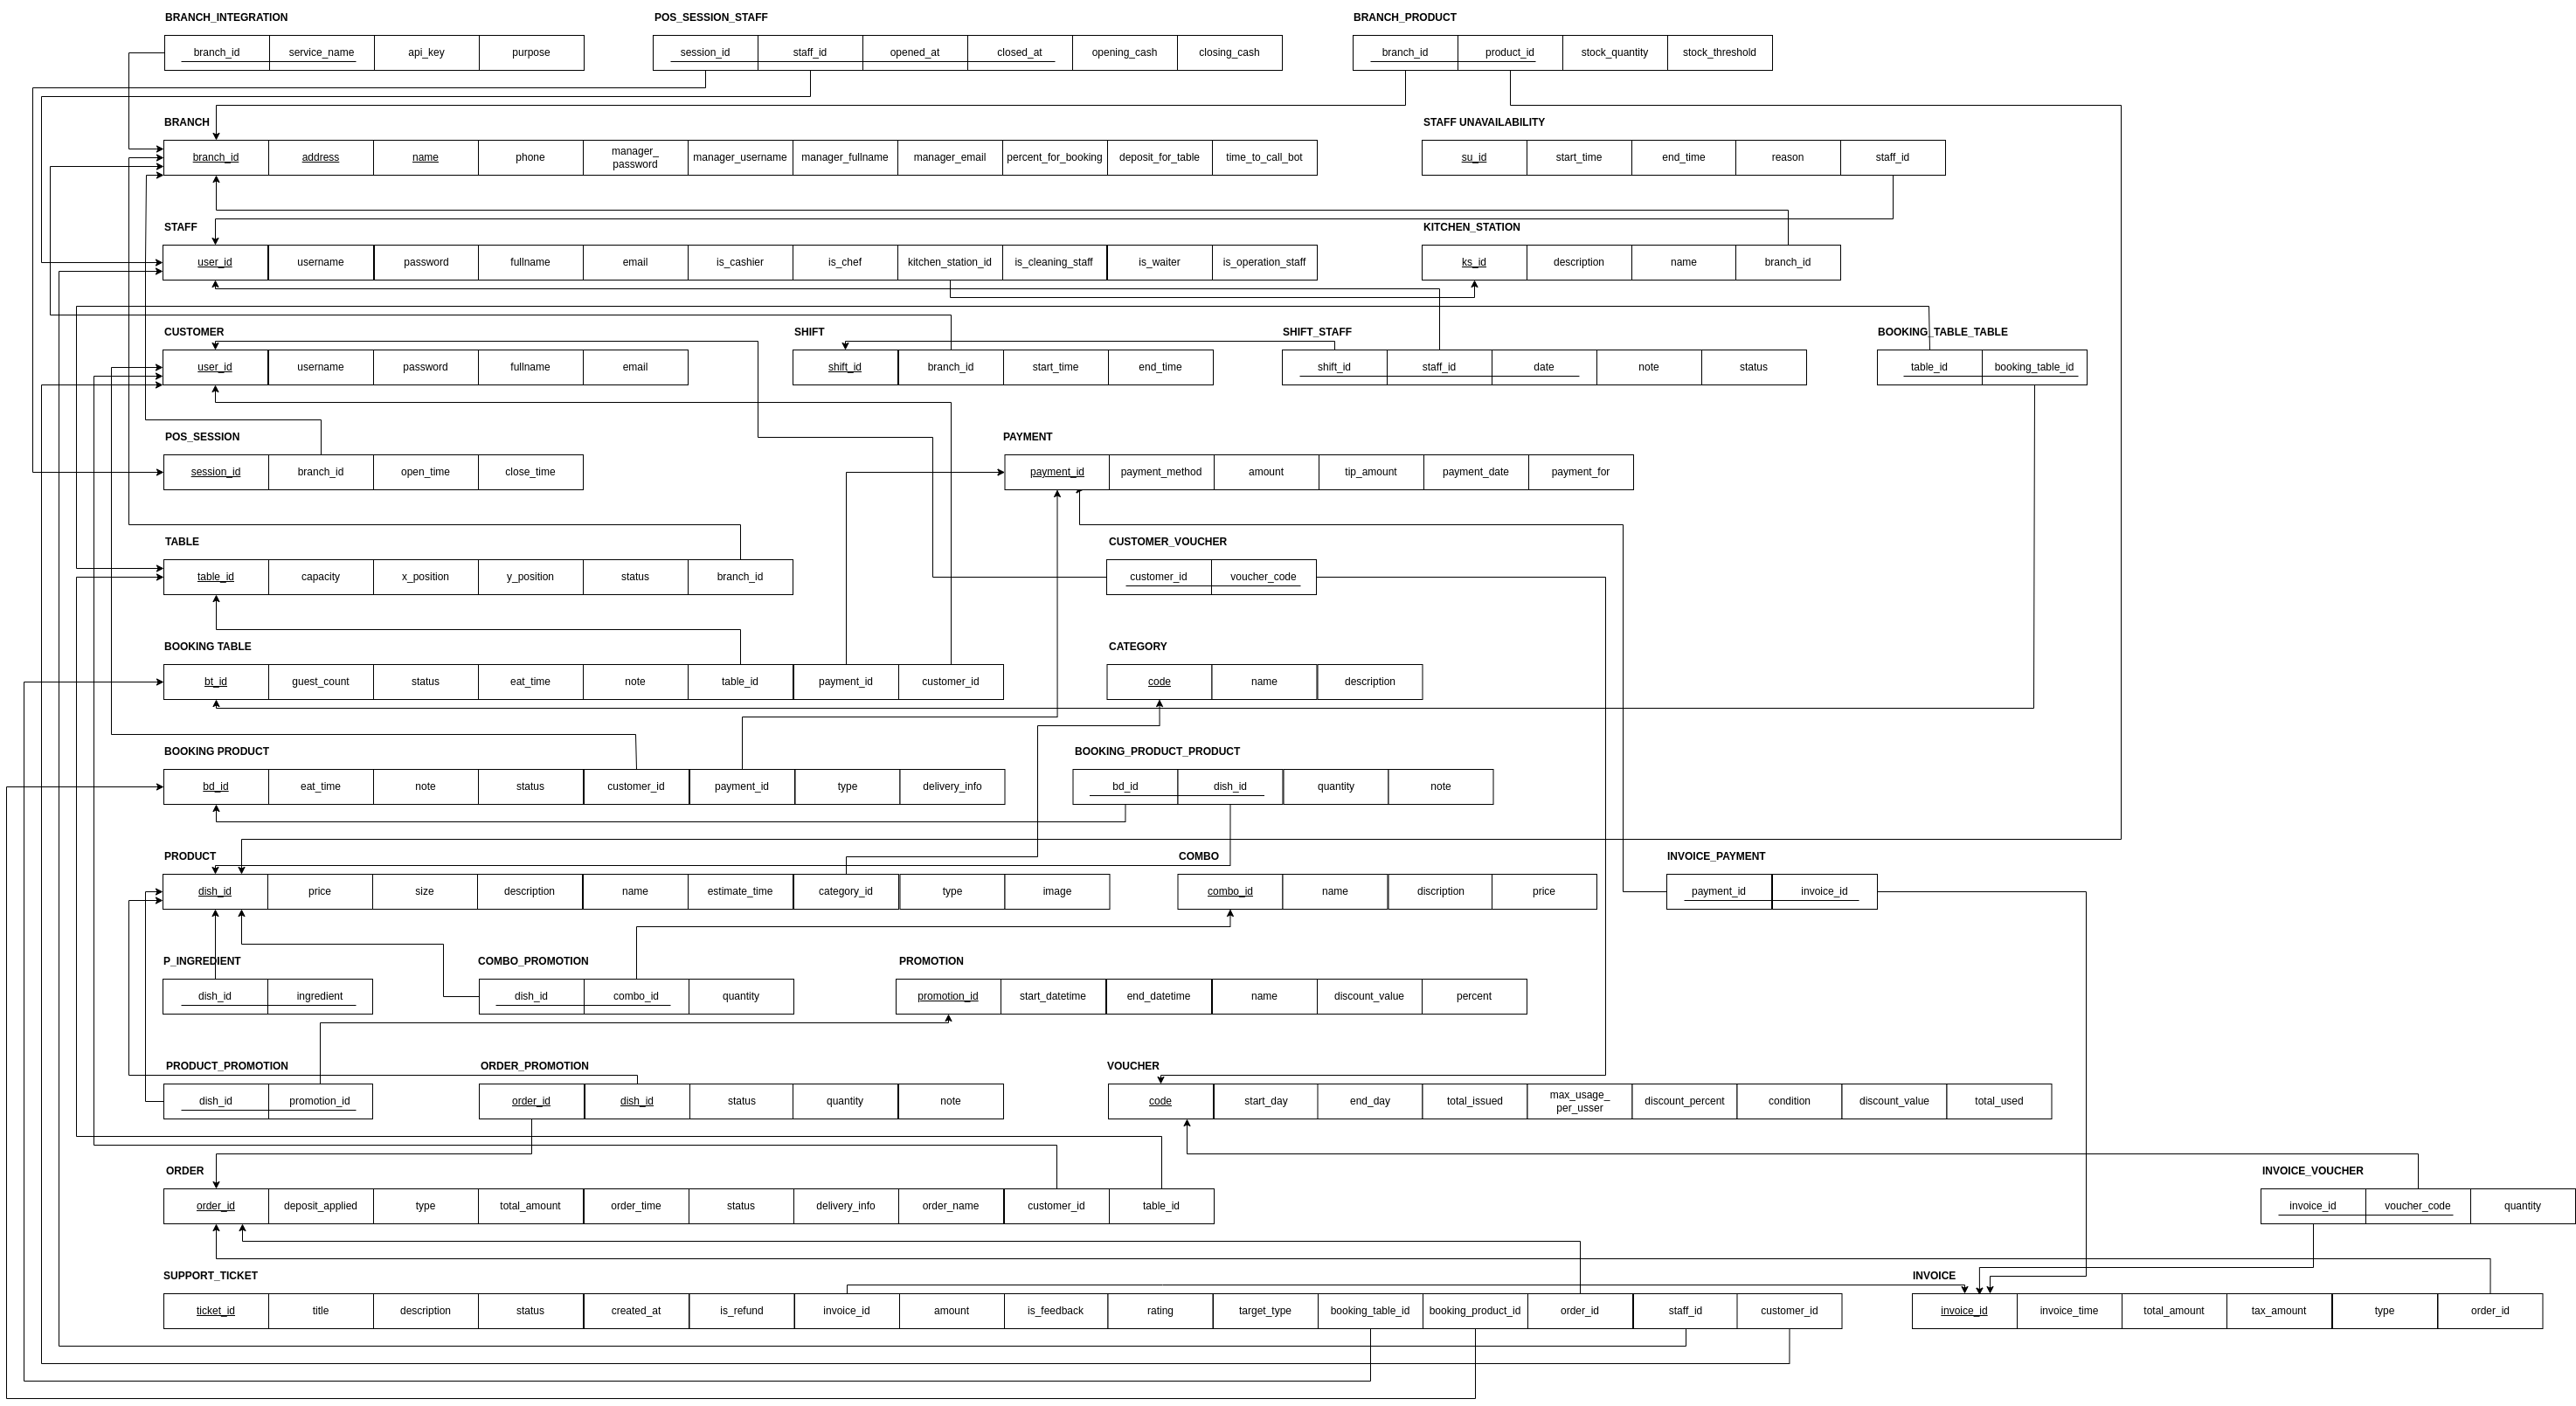
\includegraphics[height=0.9\textheight]{Images/relation.png}
    \vspace{0.5cm}
    \caption{Lược đồ quan hệ cơ sở dữ liệu luận lý}
    \label{fig:my_label}
\end{figure}

\end{landscape}


\subsubsection{Thiết kế vật lý}

Dưới đây là chi tiết thiết kế vật lý \textbf{một số bảng quan trọng} trong hệ thống. Mỗi bảng thể hiện rõ các thuộc tính, kiểu dữ liệu cụ thể, các ràng buộc và khóa ngoại (nếu có).

\begin{longtable}{|p{3.5cm}|p{3.5cm}|p{7.5cm}|}
\hline
\textbf{Thuộc tính} & \textbf{Kiểu dữ liệu} & \textbf{Ràng buộc / CHECK} \\
\hline
\endfirsthead

\hline
\textbf{Thuộc tính} & \textbf{Kiểu dữ liệu} & \textbf{Ràng buộc / CHECK} \\
\hline
\endhead

% \hline \multicolumn{4}{|r|}{{Còn tiếp ...}} \\
\hline
\endfoot

\hline
\endlastfoot

\multicolumn{3}{|l|}{\textbf{product}} \\
\hline
id & bigint & NOT NULL, PK \\
name & varchar(255) & NOT NULL \\
price & numeric(38,2) & \\
type & varchar(255) & CHECK IN ('COUNTABLE', 'UNCOUNTABLE', 'SERVICE') \\
category\_id & bigint & NOT NULL, FK \\
\hline

\multicolumn{3}{|l|}{\textbf{voucher}} \\
\hline
id & bigint & NOT NULL, PK \\
code & varchar(100) & NOT NULL \\
discount\_value & numeric(38,2) & \\
discount\_percent & double precision & \\
start\_date & date & NOT NULL \\
end\_date & date & NOT NULL \\
\hline

\multicolumn{3}{|l|}{\textbf{invoice}} \\
\hline
id & bigint & NOT NULL, PK \\
order\_id & bigint & NOT NULL, FK \\
invoice\_type & varchar(255) & CHECK IN ('NORMAL', 'MERGED', 'SPLIT') \\
total\_amount & numeric(38,2) & \\
tax\_amount & numeric(38,2) & \\
\hline

\multicolumn{3}{|l|}{\textbf{combo}} \\
\hline
id & bigint & NOT NULL, PK \\
name & varchar(255) & NOT NULL \\
price & numeric(38,2) & NOT NULL \\
\hline

\multicolumn{3}{|l|}{\textbf{orders}} \\
\hline
id & bigint & NOT NULL, PK \\
type & varchar(255) & CHECK IN ('DINE\_IN', 'TAKE\_AWAY', 'DELIVERY') \\
oder\_status & varchar(255) & CHECK IN ('PLACED', 'PREPARING', 'COMPLETED', 'CANCELLED') \\
total\_amount & numeric(38,2) & \\
customer\_id & bigint & NOT NULL, FK \\
\hline

\multicolumn{3}{|l|}{\textbf{order\_product}} \\
\hline
id & bigint & NOT NULL, PK \\
order\_id & bigint & NOT NULL, FK \\
product\_id & bigint & NOT NULL, FK \\
product\_status & varchar(255) & CHECK IN ('PENDING', 'PREPARING', 'COMPLETED', 'SERVED', 'CANCELLED') \\
\hline

\multicolumn{3}{|l|}{\textbf{restaurant\_table}} \\
\hline
id & bigint & NOT NULL, PK \\
capacity & integer & \\
table\_status & varchar(255) & CHECK IN ('AVAILABLE', 'OCCUPIED', 'NEEDS\_CLEANING') \\
table\_type & varchar(255) & CHECK IN ('STANDARD', 'VIP') \\
branch\_id & bigint & NOT NULL, FK \\
\hline

\multicolumn{3}{|l|}{\textbf{booking\_table}} \\
\hline
id & bigint & NOT NULL, PK \\
booking\_status & varchar(255) & CHECK IN ('BOOKED', 'DEPOSIT\_PAID', 'CANCELLED', 'COMPLETED') \\
time\_start & timestamp & NOT NULL \\
time\_end & timestamp & \\
customer\_id & bigint & NOT NULL, FK \\
\hline

\multicolumn{3}{|l|}{\textbf{booking\_product}} \\
\hline
id & bigint & NOT NULL, PK \\
booking\_status & varchar(255) & CHECK IN ('BOOKED', 'DEPOSIT\_PAID', 'CANCELLED', 'COMPLETED') \\
booking\_type & varchar(255) & CHECK IN ('DINE\_IN','TAKE\_AWAY','DELIVERY') \\
customer\_id & bigint & NOT NULL, FK \\
branch\_id & bigint & NOT NULL, FK \\
\hline

\multicolumn{3}{|l|}{\textbf{combo\_product}} \\
\hline
id & bigint & NOT NULL, PK \\
combo\_id & bigint & NOT NULL, FK \\
product\_id & bigint & NOT NULL, FK \\
quantity & integer & \\
\hline

\multicolumn{3}{|l|}{\textbf{invoice\_voucher}} \\
\hline
id & bigint & NOT NULL, PK \\
voucher\_id & bigint & NOT NULL, FK \\
invoice\_id & bigint & NOT NULL, FK \\
quantity & integer & \\
\hline
\end{longtable}

Sau khi hoàn thiện các bước thiết kế cơ sở dữ liệu từ mô hình khái niệm đến mô hình luận lý và vật lý, hệ thống đã được triển khai trên phần mềm quản lý cơ sở dữ liệu để trực quan hóa quan hệ giữa các bảng. Hình dưới đây thể hiện lược đồ quan hệ đầy đủ của hệ thống cơ sở dữ liệu, được xuất từ công cụ DBeaver sau khi định nghĩa và thiết lập các bảng, khóa chính, khóa ngoại và các liên kết liên quan.

\begin{figure}[H]
    \centering
    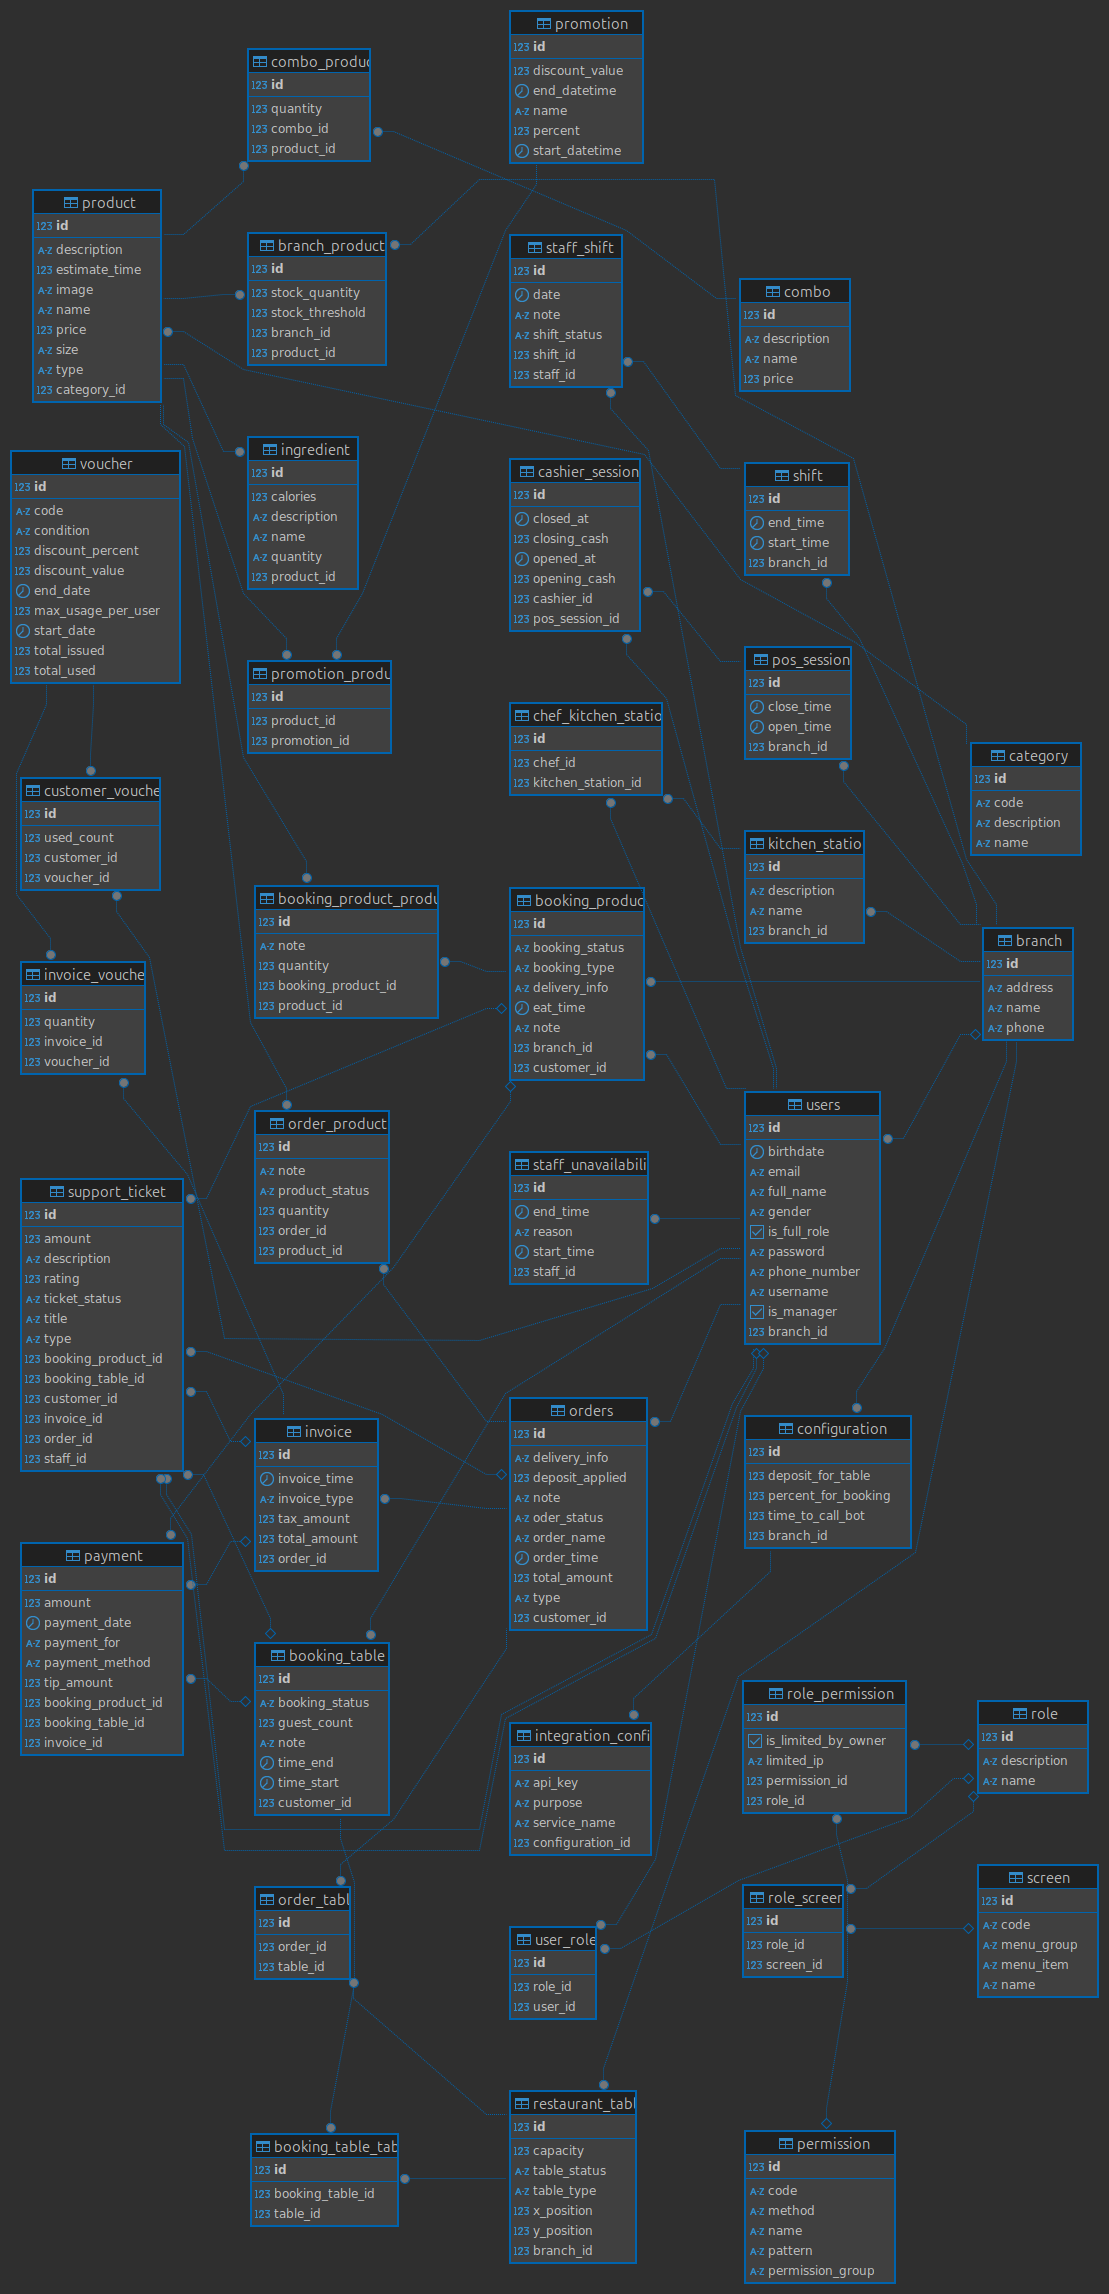
\includegraphics[height=0.9\textheight]{Images/ldqh.png}
    \vspace{0.5cm}
    \caption{Lược đồ quan hệ cơ sở dữ liệu vật lý}
    \label{fig:logical_schema}
\end{figure}
\subsection{Thiết kế giao diện}
\subsubsubsection{Module MD-01: Quản lý Lịch làm việc (Scheduling)}

\begin{figure}[H]
    \centering
    \includegraphics[width=\linewidth]{Sections/hien_thuc/img/1.1.png}
    \vspace{0.5cm}
    \caption{Giao diện Module MD-01 (1)}
    \label{fig:gantt_module_md01_1}
\end{figure}

\begin{figure}[H]
    \centering
    \includegraphics[width=\linewidth]{Sections/hien_thuc/img/1.2.png}
    \vspace{0.5cm}
    \caption{Giao diện Module MD-01 (2)}
    \label{fig:gantt_module_md01_2}
\end{figure}

\begin{figure}[H]
    \centering
    \includegraphics[width=\linewidth]{Sections/hien_thuc/img/1.3.png}
    \vspace{0.5cm}
    \caption{Giao diện Module MD-01 (3)}
    \label{fig:gantt_module_md01_3}
\end{figure}

\begin{figure}[H]
    \centering
    \includegraphics[width=\linewidth]{Sections/hien_thuc/img/1.4.png}
    \vspace{0.5cm}
    \caption{Giao diện Module MD-01 (4)}
    \label{fig:gantt_module_md01_4}
\end{figure}

\begin{figure}[H]
    \centering
    \includegraphics[width=\linewidth]{Sections/hien_thuc/img/1.5.png}
    \vspace{0.5cm}
    \caption{Giao diện Module MD-01 (5)}
    \label{fig:gantt_module_md01_5}
\end{figure}

\begin{figure}[H]
    \centering
    \includegraphics[width=\linewidth]{Sections/hien_thuc/img/1.6.png}
    \vspace{0.5cm}
    \caption{Giao diện Module MD-01 (6)}
    \label{fig:gantt_module_md01_6}
\end{figure}

\begin{figure}[H]
    \centering
    \includegraphics[width=\linewidth]{Sections/hien_thuc/img/1.7.png}
    \vspace{0.5cm}
    \caption{Giao diện Module MD-01 (7)}
    \label{fig:gantt_module_md01_7}
\end{figure}

\begin{figure}[H]
    \centering
    \includegraphics[width=\linewidth]{Sections/hien_thuc/img/1.8.png}
    \vspace{0.5cm}
    \caption{Giao diện Module MD-01 (8)}
    \label{fig:gantt_module_md01_8}
\end{figure}

\begin{figure}[H]
    \centering
    \includegraphics[width=\linewidth]{Sections/hien_thuc/img/1.9.png}
    \vspace{0.5cm}
    \caption{Giao diện Module MD-01 (9)}
    \label{fig:gantt_module_md01_9}
\end{figure}

\begin{figure}[H]
    \centering
    \includegraphics[width=\linewidth]{Sections/hien_thuc/img/1.10.png}
    \vspace{0.5cm}
    \caption{Giao diện Module MD-01 (10)}
    \label{fig:gantt_module_md01_10}
\end{figure}

\begin{figure}[H]
    \centering
    \includegraphics[width=\linewidth]{Sections/hien_thuc/img/1.11.png}
    \vspace{0.5cm}
    \caption{Giao diện Module MD-01 (11)}
    \label{fig:gantt_module_md01_11}
\end{figure}

\begin{figure}[H]
    \centering
    \includegraphics[width=\linewidth]{Sections/hien_thuc/img/1.12.png}
    \vspace{0.5cm}
    \caption{Giao diện Module MD-01 (12)}
    \label{fig:gantt_module_md01_12}
\end{figure}


\subsubsubsection{Module MD-02: Quản lý Thực đơn \& Sản phẩm}
\subsection{Thiết kế API}

Hệ thống được thiết kế theo kiến trúc RESTful API, đảm bảo khả năng mở rộng, dễ tích hợp và bảo trì. Tài liệu API chi tiết được công bố tại đường dẫn:
\url{https://app.swaggerhub.com/apis-docs/atn-903/MenuPlus/1.0.0#/}

Dưới đây là một số API tiêu biểu minh hoạ cho các chức năng chính trong hệ thống:

\begin{figure}[H]
\centering
\includegraphics[width=15cm]{Images/Screenshot from 2025-05-10 17-03-23.png}
\vspace{0.5cm}
\caption{API quản lý Thực đơn và Sản phẩm (Menu & Product API)}
\label{fig:api_menu_product}
\end{figure}

\begin{figure}[H]
\centering
\includegraphics[width=15cm]{Images/Screenshot from 2025-05-10 17-03-40.png}
\vspace{0.5cm}
\caption{API quản lý Lịch làm việc (Scheduling API)}
\label{fig:api_scheduling}
\end{figure}

\begin{figure}[H]
\centering
\includegraphics[width=15cm]{Images/Screenshot from 2025-05-10 17-03-52.png}
\vspace{0.5cm}
\caption{API đặt bàn (Booking API)}
\label{fig:api_booking}
\end{figure}

\begin{figure}[H]
\centering
\includegraphics[width=15cm]{Images/Screenshot from 2025-05-10 17-04-05.png}
\vspace{0.5cm}
\caption{API hệ thống điểm bán (POS API)}
\label{fig:api_pos}
\end{figure}

\begin{figure}[H]
\centering
\includegraphics[width=15cm]{Images/Screenshot from 2025-05-10 17-04-34.png}
\vspace{0.5cm}
\caption{API hệ thống bếp và giao hàng (KDS & Delivery API)}
\label{fig:api_kds_delivery}
\end{figure}



% \subsection{Thiết kế cơ sở dữ liệu}
ER diagram là công cụ hữu hiệu giúp kiểm tra tính nhất quán và hoàn thiện trong thiết kế cơ sở dữ liệu. Nếu có sai sót hoặc mâu thuẫn trong hiểu biết ban đầu về hệ thống, chúng có thể được phát hiện và sửa chữa kịp thời thông qua ER diagram. Điều này góp phần loại bỏ các lỗi thiết kế và tối ưu hóa cơ sở dữ liệu.

\subsubsection{Bảng mô tả các schema}
Dưới đây là các bảng mô tả thuộc tính của các schema có trong lược đồ cơ sở dữ liệu quan hệ:

\begin{table}[H]
\centering
\renewcommand{\arraystretch}{1.5}
\begin{tabular}{|l|p{7cm}|p{4cm}|}
\hline
\textbf{Thuộc tính mô tả} & \textbf{Mô tả} & \textbf{Kiểu dữ liệu} \\
\hline
user\_id & ID của người dùng & bigint \\
\hline
username & Username của người dùng & varchar(255) \\
\hline
email & Email của người dùng & varchar(255) \\
\hline
password & Mật khẩu của người dùng đã được hash & varchar(255) \\
\hline
avatar\_url & URL dẫn đến avatar của người dùng & varchar(255) \\
\hline
user\_type & Loại người dùng (recruiter, candidate) & enum \\
\hline
\end{tabular}
\caption{Users Schema}
\end{table}


% \subsection{Quản lí source code}
 % phần này ghi cách làm việc với source code của nhóm: quy trình làm việc nhóm chuẩn: tạo nhánh -> làm -> đẩy code -> tạo merge req -> review -> merge. 

Ở đồ án này, nhóm sử dụng GitHub để quản lý sourcce code và tương tác với các thành viên khác. Nhằm tạo sự thống nhất, tiện lợi và hiệu quả trong quá trình làm việc nhóm với source code, chúng ta sẽ sử dụng \textbf{GitHub flow branching strategy } được đề xuất bởi chính GitHub. \\
% Nhớ tạo ref cho cái này https://docs.github.com/en/get-started/quickstart/github-flow

GitHub flow branching strategy là một quy trình làm việc tương đối đơn giản cho phép các nhóm nhỏ hoặc các ứng dụng/sản phẩm web không yêu cầu hỗ trợ nhiều phiên bản để nhanh chóng hoàn thành công việc của họ. \\

Trong GitHub flow, nhánh chính chứa mã nguồn đã sẵn sàng cho sản xuất. Các nhánh khác, được gọi là nhánh tính năng, nên chứa công việc về các tính năng mới và sửa lỗi, và sẽ được hợp nhất trở lại nhánh chính khi công việc hoàn thành và được đánh giá đúng cách. 
\subsubsection{GitHub Flow Best Practices}
Khi làm việc với chiến lược GitHub flow branching, có sáu nguyên tắc cần nên tuân thủ để đảm bảo duy trì mã nguồn tốt:
\begin{itemize}
    \item Mọi mã nguồn trong nhánh main nên có thể triển khai.
    \item Tạo các nhánh mới có tên mô tả rõ ràng từ nhánh chính để thực hiện công việc mới, chẳng hạn như features/add-new-payment-types.
    \item Commit công việc mới vào các nhánh local và thường xuyên push công việc lên remote.
    \item Để yêu cầu phản hồi hoặc sự giúp đỡ, hoặc khi nghĩ rằng công việc của mình đã sẵn sàng để hợp nhất vào nhánh chính, mở một pull request.
    \item Sau khi công việc hoặc tính năng của bạn đã được xem xét và chấp nhận, nó có thể được hợp nhất vào nhánh main.
    \item Sau khi công việc đã được hợp nhất vào nhánh main, nó nên được triển khai ngay lập tức.
\end{itemize}

\subsubsection{GitHub Flow: Lợi ích và nhược điểm}
\begin{figure}[H]
    \centering
    \includegraphics[width=8cm]{Images/githubflow.png}
    \vspace{0.5cm}
    \caption{Mô phỏng các branch trong 1 GitHub flow}
\end{figure}
\begin{itemize}
    \item Lợi ích:
    \begin{itemize}
    \item Do tính đơn giản của quy trình làm việc, chiến lược này cho phép triển khai liên tục và tích hợp liên tục.
    \item Chiến lược này hoạt động tốt cho các nhóm nhỏ và ứng dụng web.
    \end{itemize}

    \item Nhược điểm: 
    \begin{itemize}
    \item Chiến lược này không thể hỗ trợ nhiều phiên bản mã nguồn cùng một lúc trên môi trường production.
    \item Sự thiếu hụt các nhánh phát triển riêng biệt khiến cho GitHub Flow trở nên dễ bị ảnh hưởng bởi lỗi trong môi trường production.
    \end{itemize}
\end{itemize}

\subsubsection{Các bước trong GitHub flow}
Khi cần thực hiện một tính năng mới trong hệ thống thì mỗi thành viên phải hoàn thiện hết các bước cần thiết như sau.
\begin{enumerate}
    \item \textbf{Tạo nhánh}
    \begin{itemize}
        \item Tạo một nhánh trong repository. Một tên nhánh ngắn gọn và mô tả sẽ giúp mọi gnười dễ dàng nhìn thấy công việc đang diễn ra và dựa theo cú pháp sau: features/{feature-description} 
        \item Bằng cách tạo một nhánh, bạn tạo ra một không gian để làm việc mà không ảnh hưởng đến nhánh mặc định. Ngoài ra, điều này cũng tạo cơ hội cho mọi người xem xét công việc của bạn.
    \end{itemize}

    \item \textbf{Thực hiện các thay đổi}
    \begin{itemize}
        \item Nhánh của bạn là một nơi an toàn để thực hiện các thay đổi. Nếu bạn mắc lỗi, bạn có thể hoàn nguyên các thay đổi hoặc đẩy các thay đổi bổ sung để sửa lỗi. Các thay đổi của bạn sẽ không xuất hiện trên nhánh mặc định cho đến khi bạn hợp nhất nhánh của mình.
        \item Commit và đẩy các thay đổi lên nhánh của bạn. Đặt một thông điệp mô tả cho mỗi commit để giúp bạn và các đóng góp viên trong tương lai hiểu rõ những thay đổi mà commit chứa. Ví dụ, "fix typo" hoặc "increase rate limit". 
        \item Lý tưởng là mỗi commit chứa một thay đổi độc lập, hoàn chỉnh. Điều này giúp dễ dàng hoàn nguyên các thay đổi nếu bạn quyết định thay đổi hướng tiếp cận. Ví dụ, nếu bạn muốn đổi tên một biến và thêm một số tests, hãy đặt thay đổi tên biến trong một commit và các tests trong một commit khác. Sau này, nếu bạn muốn giữ lại các tests nhưng hoàn nguyên thay đổi tên biến, bạn có thể hoàn nguyên commit cụ thể chứa thay đổi tên biến. Nếu bạn đặt thay đổi tên biến và tests trong cùng một commit hoặc phân tán thay đổi tên biến qua nhiều commit, bạn sẽ phải mất nhiều công sức hơn để hoàn nguyên các thay đổi của mình.
        \item Bằng cách commit và đẩy các thay đổi của bạn, bạn sao lưu công việc của mình lên lưu trữ từ xa. Điều này có nghĩa là bạn có thể truy cập công việc của mình từ bất kỳ thiết bị nào. Đồng thời, mọi người cũng có thể xem công việc của bạn, trả lời câu hỏi, và đưa ra đề xuất hoặc đóng góp.
        \item Tiếp tục thực hiện, commit, và đẩy các thay đổi lên nhánh của bạn cho đến khi bạn sẵn sàng để yêu cầu phản hồi.
    \end{itemize}
    

    \item \textbf{Tạo pull request}
    \begin{itemize}
        \item Tạo một pull request để yêu cầu đồng đội đưa ra phản hồi về các thay đổi của bạn. Phản hồi từ việc xem xét pull request là rất quan trọng, đến nỗi một số repository yêu cầu một xem xét chấp thuận trước khi có thể hợp nhất pull request. Nếu bạn muốn có phản hồi sớm hoặc tư vấn trước khi hoàn tất các thay đổi của bạn, bạn có thể đánh dấupull request của mình như một bản "draft".

        \item Khi bạn tạo một pull request, bao gồm một tóm tắt về các thay đổi và vấn đề nào mà chúng giải quyết. Bạn có thể bao gồm hình ảnh, liên kết và bảng để giúp truyền đạt thông tin này. Nếu pull request của bạn liên quan đến một vấn đề, hãy liên kết vấn đề để những người liên quan đến vấn đề biết về pull request và ngược lại. Nếu bạn liên kết với một từ khóa, vấn đề sẽ tự động đóng khi pull request được hợp nhất.
    
        \item Ngoài việc điền thông tin vào thân yêu cầu pull, bạn có thể thêm bình luận vào các dòng cụ thể của pull request để chỉ ra rõ điều gì đó đối với người xem xét. 
    
        \item Repository của bạn có thể được cấu hình tự động yêu cầu xem xét từ các nhóm hoặc người dùng cụ thể khi một pull request được tạo. Bạn cũng có thể thêm bằng cách \textbf{@đề cập} hoặc yêu cầu xem xét từ các người hoặc nhóm cụ thể. 
    
        \item Nếu repository của bạn đã cấu hình để chạy kiểm tra trạng thái trên các pull request, bạn sẽ thấy bất kỳ kiểm tra nào thất bại trên pull request của bạn. Điều này giúp bạn phát hiện lỗi trước khi hợp nhất nhánh của mình. 
    \end{itemize}

    \item \textbf{Giải quyết review comments}
    \begin{itemize}
        \item Người xem xét nên để lại câu hỏi, ý kiến và gợi ý. Người xem xét có thể bình luận về toàn bộ pull request hoặc thêm bình luận vào các dòng hoặc tệp tin cụ thể. Bạn và người xem xét có thể chèn hình ảnh hoặc đề xuất mã nguồn để làm rõ ý kiến.
        \item Bạn có thể tiếp tục commit và đẩy các thay đổi phản hồi. Pull request của bạn sẽ được cập nhật tự động.
    \end{itemize}

    \item \textbf{Merge pull request}
    \begin{itemize}
        \item Khi pull request của bạn được chấp thuận, bạn có thể merge pull request vào nhánh main. Điều này sẽ tự động hợp nhất nhánh của bạn để các thay đổi của bạn xuất hiện trên nhánh mặc định. GitHub giữ lại lịch sử của bình luận và commit trong pull request để giúp đội ngũ đóng góp viên trong tương lai hiểu rõ các thay đổi của bạn.
        \item GitHub sẽ thông báo nếu pull request của bạn có xung đột cần giải quyết trước khi hợp nhất. 
        \item Cài đặt bảo vệ nhánh có thể ngăn chặn quá trình hợp nhất nếu pull request của bạn không đáp ứng một số yêu cầu nhất định. Ví dụ, bạn cần một số lượng xác nhận đánh giá hoặc một đánh giá chấp thuận từ một nhóm cụ thể.
    \end{itemize}

    \item \textbf{Xóa nhánh đã được merge}
    \begin{itemize}
        \item Sau khi hợp nhất pull request của bạn, hãy xóa nhánh của bạn. Điều này chỉ ra rằng công việc trên nhánh đã hoàn tất và ngăn chặn bạn hoặc người khác sử dụng nhánh cũ một cách tình cờ.
        \item Đừng lo lắng về việc mất thông tin. Pull request và lịch sử commit của bạn sẽ không bị xóa. Bạn luôn có thể khôi phục lại nhánh bị xóa hoặc hoàn nguyên pull request nếu cần thiết.
    \end{itemize}    
\end{enumerate}

\subsection{Thiết kế giao diện người dùng}
Như đã biết, phần front-end web của ứng dụng demo của nhóm được phát triển bằng ReactJS, sử dụng TypeScript như ngôn ngữ lập trình. Cấu trúc giao diện web là một khía cạnh quan trọng trong quá trình phát triển phần front-end, ảnh hưởng trực tiếp tới việc phát triển, bảo trì và mở rộng ứng dụng.\\

Hiện nay trên thế giới có nhiều phương pháp để xây dựng cấu trúc giao diện web như: feature-based, component-based, module-based, Atomic Design...Mỗi phương pháp đều có ưu nhược điểm riêng phù hợp với từng loại dự án.\\

Phương pháp mà nhóm sẽ áp dụng để viết cấu trúc giao diện của ứng dụng demo là phương pháp feature-based. Theo đó, giao diện sẽ được chia thành các component dựa trên từng tính năng/chức năng của ứng dụng. Mỗi component sẽ quản lý render và xử lý logic riêng cho từng tính năng.
\subsubsection{Tại sao sử dụng cấu trúc Feature-Based}
Khi phát triển ứng dụng React, việc sử dụng cách tổ chức folder theo tính năng (feature-based) mang lại nhiều lợi ích. Dưới đây là một số lý do tại sao nên áp dụng cách tổ chức này:

\begin{itemize}
    \item Dễ quản lý và mở rộng: Tách biệt các tính năng hoặc thành phần (component) thành các folder riêng biệt giúp quản lý dễ dàng hơn khi ứng dụng phát triển lớn dần. Mỗi tính năng được xem như một module độc lập, có thể quản lý và phát triển riêng biệt mà không ảnh hưởng đến các tính năng khác. Điều này giúp đảm bảo tính tổ chức và cấu trúc của dự án, giúp nhóm phát triển dễ dàng tìm kiếm và chỉnh sửa mã nguồn.
    \item Dễ mở rộng và sửa đổi tính năng: Với cách tổ chức feature-based, việc thêm, xóa hoặc cập nhật tính năng trở nên dễ dàng hơn. Bằng cách tách riêng từng tính năng thành các folder, nhóm phát triển có thể làm việc trên một tính năng cụ thể mà không cần quan tâm đến các tính năng khác. Điều này giúp giảm thiểu xung đột và rủi ro gây lỗi khi thay đổi mã nguồn.
    \item Dễ tái sử dụng code: Khi mỗi tính năng được tách ra thành một package độc lập, code trong từng tính năng có thể dễ dàng tái sử dụng giữa các dự án khác nhau. Điều này tạo điều kiện thuận lợi cho việc chia sẻ và sử dụng lại code, giúp tiết kiệm thời gian và công sức phát triển.
    \item Giảm sự phức tạp khi tổ chức theo loại component: Thay vì tổ chức theo loại component như components, containers, reducers, việc sắp xếp theo tính năng giúp giảm sự phức tạp của dự án. Code được tổ chức theo tính năng, giúp tăng tính nhất quán và dễ đọc, hiểu và bảo trì hơn. Nhóm phát triển có thể tập trung vào từng tính năng cụ thể mà không phải lo lắng về cấu trúc tổ chức.
    \item Kiểm soát và giới hạn sự phụ thuộc: Cách tổ chức feature-based giúp áp dụng quy tắc về tính khả dụng của các component. Điều này giúp kiểm soát và giới hạn sự phụ thuộc lẫn nhau giữa các tính năng, tránh ảnh hưởng không mong muốn khi thay đổi. Đồng thời, giúp cải thiện khả năng kiểm thử và tái sử dụng code.
    \item Hỗ trợ phát triển ứng dụng lớn và phức tạp: Cách tổ chức feature-based thích hợp cho việc phát triển ứng dụng lớn, có nhiều tính năng phức tạp. Nó giúp tăng tính tổ chức, quản lý và tiếp cận dự án, giảm thiểu sự mất rối và mâu thuẫn khi làm việc với nhiều thành viên cùng một lúc.
\end{itemize}
Có một số lý do tại sao cách tổ chức feature-based có ưu điểm hơn cách tổ chức theo loại thành phần như cách tổ chức theo loại thành phần như actions, components, containers khi dự án phát triển lớn:

\begin{itemize}
    \item Về tính khả dụng: Khi tổ chức theo loại thành phần, các thành phần có thể sử dụng lẫn nhau một cách tùy tiện. Điều này dễ dẫn đến sự phụ thuộc chéo không cần thiết giữa các module. Còn cách feature-based giới hạn tính khả dụng của thành phần trong phạm vi tính năng/module riêng, tránh được vấn đề này.
   
    \item Về tái sử dụng: Khi tổ chức theo tính năng, mỗi tính năng trở thành một package/module độc lập có thể dễ dàng tái sử dụng trong các dự án khác. Còn cách theo loại thành phần thì khó tái sử dụng riêng lẻ từng thành phần.
   
    \item Về bảo trì: Khi dự án lớn, việc quản lý theo từng tính năng thay vì loại thành phần sẽ đơn giản và rõ ràng hơn. Dễ dàng tìm kiếm, thêm bớt các tính năng một cách độc lập.
    
    \item Về mở rộng: Cách feature-based cho phép mở rộng từng tính năng độc lập mà không ảnh hưởng đến các tính năng khác. Trong khi đó, cách theo loại thành phần dễ dẫn đến tình trạng phức tạp khi mở rộng.
\end{itemize}

Do đó, cách tổ chức feature-based thích hợp hơn khi quy mô dự án lớn về mặt tính khả dụng, tái sử dụng, bảo trì và khả năng mở rộng.\\

Do vậy nhóm chọn cách tổ chức theo feature-based cho trang web demo của nhóm.
\subsubsection{Cấu trúc phần UI}
Cách tổ chức này chia ứng dụng thành các thư mục chính, mỗi thư mục đại diện cho một tính năng cụ thể trong ứng dụng. Đây là một cách tiếp cận phổ biến trong việc tổ chức dự án, giúp tăng tính tổ chức và dễ quản lý.

\begin{itemize}
    \item \textbf{Thư mục "Components":}\\
    Thư mục này chứa các thành phần (components) của ứng dụng. Các thành phần có thể được định nghĩa dưới dạng các file độc lập hoặc nhóm lại thành các thư mục con. Điều này cho phép bạn xây dựng các thành phần con bên trong một thành phần cha, giúp quản lý và sử dụng lại mã nguồn một cách dễ dàng.
    \item \textbf{Thư mục "Scenes":}\\
    Thư mục này chứa các trang hoặc màn hình trong ứng dụng. Các scenes có thể bao gồm các thành phần, scenes và services khác. Điều này cho phép bạn tổ chức các thành phần trong một ngữ cảnh cụ thể và quản lý logic của từng màn hình một cách rõ ràng.
    \item \textbf{Thư mục "Services":}\\
    Thư mục này chứa các module phục vụ logic ứng dụng. Các module này có thể được sử dụng để xử lý các tác vụ như xử lý dữ liệu, gọi API hoặc thao tác với cơ sở dữ liệu. Tổ chức các module theo thư mục này giúp tách biệt và quản lý tốt hơn các chức năng trong ứng dụng.

\end{itemize}
    Mỗi tính năng hoặc chức năng của ứng dụng sẽ được đặt trong một thư mục riêng biệt, bao gồm tất cả những gì cần thiết để tính năng đó hoạt động. Điều này giúp tăng tính tổ chức và khả năng tìm kiếm mã nguồn liên quan đến từng tính năng cụ thể.\\

Nhóm dựa vào những tìm hiểu ở trên đây để tiến hành xây dựng cấu trúc của ứng dụng. Cấu trúc thư mục của dự án có thể được tổ chức như sau:

\begin{itemize}
    \item \textbf{apis:} Thư mục chứa các tệp tin liên quan đến việc gọi API.
    \item \textbf{assets:} Thư mục chứa các tài nguyên như hình ảnh, file đính kèm và các tài liệu khác sử dụng trong ứng dụng.
    \item \textbf{components:} Thư mục chứa các thành phần React, được sắp xếp theo cấu trúc phân cấp cho phép định nghĩa các component con bên trong component cha.
    \item \textbf{constants:} Thư mục chứa các hằng số và cấu hình cho dự án.
    \item \textbf{hooks:} Thư mục chứa các custom hooks, đây là các hàm tái sử dụng giúp quản lý trạng thái và logic trong ứng dụng.
    \item \textbf{layouts:} Thư mục chứa các layout hoặc template để sắp xếp giao diện của ứng dụng.
    \item \textbf{libs:} Thư mục chứa các thư viện và công cụ bên thứ ba được sử dụng trong dự án.
    \item \textbf{pages:} Thư mục chứa các trang hoặc màn hình trong ứng dụng, tương đương với scenes.
    \item \textbf{routes:} Thư mục chứa các tệp tin liên quan đến định tuyến trong ứng dụng.
    \item \textbf{styles:} Thư mục chứa các tệp tin CSS hoặc SCSS để định nghĩa kiểu dáng cho các component.
    \item \textbf{types:} Thư mục chứa các tệp tin liên quan đến kiểu dữ liệu và khai báo cho TypeScript.
\end{itemize}
Với cấu trúc thư mục này, dự án của bạn được tổ chức một cách rõ ràng và dễ quản lý. Mỗi thành phần có vị trí và chức năng riêng, giúp tăng tính tái sử dụng và dễ bảo trì trong quá trình phát triển.
\subsubsection{Cách các thành phần tương tác với nhau}
Trong cấu trúc feature-based, các thành phần chính sẽ tương tác với nhau một cách rõ ràng và có trình tự nhất định. Dưới đây là mô tả chi tiết về cách các thành phần này tương tác:

\begin{itemize}
    \item Components (Thành phần): Components được sử dụng trong Scenes và Pages để xây dựng giao diện người dùng. Chúng có thể bao gồm các thành phần con bên trong, tạo ra một cấu trúc phân cấp. Components có khả năng nhận thông tin từ các props và trả về các thành phần UI tương ứng.
    \item Scenes và Pages: Scenes và Pages là các trang hoặc màn hình trong ứng dụng, chứa các Components. Chúng là nơi tổ chức và sắp xếp các Components để hiển thị giao diện người dùng. Scenes và Pages có thể sử dụng Services để truy xuất dữ liệu và xử lý logic nghiệp vụ.
    \item Services (Dịch vụ): Services là các modules hoặc lớp được sử dụng để thực hiện các tác vụ như gọi API, xử lý logic phức tạp, hoặc truy xuất dữ liệu từ nguồn ngoài. Components, Scenes, và Pages có thể sử dụng Services để gửi yêu cầu và nhận kết quả từ các hoạt động này.
    \item Actions (Hành động): Actions là các sự kiện được phát ra từ Components, Scenes và Services khi có sự kiện xảy ra, ví dụ như người dùng click vào một nút hoặc hoàn thành một form. Actions mô tả hành động cần thực hiện và có thể chứa dữ liệu liên quan.
    \item Reducers (Bộ giảm nhẹ): Reducers là các hàm xử lý Actions để cập nhật trạng thái ứng dụng lưu trữ trong store. Khi một Action được gửi đi, Reducers sẽ xác định cách cập nhật trạng thái hiện tại và trả về một trạng thái mới.
    \item Store (Kho lưu trữ): Store là nơi lưu trữ trạng thái toàn cục của ứng dụng. Nó chứa các Reducers và cung cấp các phương thức để truy cập và cập nhật trạng thái. Store có thể được truy cập bởi tất cả các thành phần trong ứng dụng.
    \item Hooks (Các hàm tái sử dụng): Components, Scenes, và Services có thể sử dụng các Hooks custom để quản lý logic phức tạp hơn. Hooks cho phép tái sử dụng mã logic và trạng thái trong các Components và Scenes mà không cần sử dụng các lớp (class) React.
    \item Assets (Tài nguyên): Assets bao gồm các tệp tin như hình ảnh, các tài liệu đính kèm, các tệp tin CSS hoặc SCSS, v.v. Các thành phần như Components, Scenes và Services có thể sử dụng Assets để xây dựng giao diện và logic trong ứng dụng.
\end{itemize}

Tóm lại, cấu trúc feature-based cho phép các thành phần trong ứng dụng tương tác một cách rõ ràng và có trình tự nhất định. Thông qua việc sử dụng các phương thức như props, Actions, Reducers, và Hooks, dữ liệu và logic được truyền và xử lý một cách mạch lạc và dễ dàng quản lý.

\subsubsection{Kết quả thiết kế giao diện Website}
\subsubsubsection{Màn hình Home}

% \subsection{Triển khai Web API cho cơ sở dữ liệu}

\subsubsection{Triển khai Backend}
Nhóm đã áp dụng mô hình MVC (Model-View-Controller) trong việc xây dựng phần Backend cho ứng dụng của mình. Trong mô hình MVC, mỗi đối tượng sẽ có ba thành phần chính là Controller, Model và View (Router) để đảm bảo tính phân tách và dễ bảo trì của ứng dụng.
\begin{itemize}
    \item Controller: Đây là thành phần chịu trách nhiệm xử lý yêu cầu từ phía client và điều khiển việc xử lý của ứng dụng. Controller sẽ nhận các yêu cầu từ phía client, xử lý chúng và gửi kết quả trả về cho client. Controller cũng có thể gọi các phương thức của Model để thực hiện các thao tác truy vấn cơ sở dữ liệu.
    \item Model: Đây là thành phần đại diện cho dữ liệu và xử lý các thao tác truy vấn cơ sở dữ liệu. 
    \item View (Router): Đây là thành phần đại diện cho giao diện người dùng. View sẽ nhận các yêu cầu từ phía client và điều hướng chúng đến các Controller tương ứng. View cũng có thể chứa các template để hiển thị dữ liệu trả về từ Controller.
\end{itemize}

% \subsubsection{Deploy}


% \newpage
% \section{TỔNG KẾT}


% \newpage
% \section{KẾ HOẠCH PHÁT TRIỂN}

Để đảm bảo tiến độ và chất lượng của phần mềm quản lý đặt món nhà hàng, kế hoạch phát triển được xây dựng chi tiết, phân chia thành các giai đoạn rõ ràng cho từng chức năng chính. Kế hoạch này được thể hiện qua các biểu đồ Gantt, mô tả thời gian thực hiện và các mốc quan trọng trong quá trình phát triển. Chi tiết kế hoạch có thể được xem tại: \url{https://byvn.net/fze2}.

\begin{figure}[H]
    \centering
    \includegraphics[width=\linewidth]{Images/gantt_1}
    \vspace{0.5cm}
    \caption{Biểu đồ Gantt cho các chức năng Quản lý thực đơn - sản phẩm và Hệ thống POS Ăn tại chỗ}
    \label{fig:gantt_menu_pos}
\end{figure}

\begin{figure}[H]
    \centering
    \includegraphics[width=\linewidth]{Images/gantt_2}
    \vspace{0.5cm}
    \caption{Biểu đồ Gantt cho các chức năng Hệ thống POS Mang về và Giao hàng}
    \label{fig:gantt_takeaway_delivery}
\end{figure}

\begin{figure}[H]
    \centering
    \includegraphics[width=\linewidth]{Images/gantt_3}
    \vspace{0.5cm}
    \caption{Biểu đồ Gantt cho các chức năng Tích hợp bếp và Đặt bàn/món trước}
    \label{fig:gantt_kitchen_booking}
\end{figure}

\begin{figure}[H]
    \centering
    \includegraphics[width=\linewidth]{Images/gantt_4}
    \vspace{0.5cm}
    \caption{Biểu đồ Gantt cho các chức năng Quản lý lịch, Báo cáo, Xác nhận bot và Kiểm thử}
    \label{fig:gantt_schedule_report_test}
\end{figure}
% \newpage



% \section{TRIỂN KHAI HỆ THỐNG}
\subsection{Triền khai Front-end}
Như đã được đề cập, nhóm triển khai hệ thống lên nền tảng Vercel nhằm tối ưu chi phí và tận dụng những lợi ích liên quan đến việc thống kê trang web. Việc triển khai lên Vercel có thể được thực hiện qua các bước sau:
\begin{itemize}
    \item Đăng ký và tạo tài khoản Vercel: Đầu tiên, nhóm sẽ đăng ký một tài khoản trên Vercel. Quá trình này thường đơn giản và chỉ đòi hỏi thông tin cơ bản như địa chỉ email và mật khẩu hoặc có thể sử dụng Github làm tài khoản.
    \item Tạo dự án trên Vercel: Sau khi có tài khoản, nhóm sẽ tạo một dự án mới trên Vercel. Điều này thường liên quan đến việc cung cấp tên dự án và liên kết đến kho lưu trữ mã nguồn, chẳng hạn như GitHub hoặc GitLab.
    \item Cấu hình dự án: Trong quá trình tạo dự án, nhóm sẽ phải cấu hình các thông số cho dự án trên Vercel. Điều này có thể bao gồm chỉ định các biến môi trường, xác định cách triển khai và xử lý các bước xây dựng. \\
    
    Các cấu hình của nhóm cho phần front-end của dự án như sau: 
    \begin{itemize}
        \item $Build Command$: next build
        \item $Output Directory$: Next.js default
        \item $Install Command$: yarn
        \item $Development Command$: next
        \item $Node.js Version$: 18.18
        \item $NEXT\_PUBLIC\_GOOGLE\_SITE\_VERIFICATION$: hbwzV-DeoMMsgwNxZaw6s9L74x53\_w8KjhK68izrsnE
        \item $NEXT\_PUBLIC\_GOOGLE\_MEASUREMENT\_ID$: G-MDBKYG0VYG
        \item $CLIENT\_URL$: https://share-cv.vercel.app
        \item $SERVER\_URL$: https://share-cv-ubv1.onrender.com
    \end{itemize}
    \item Triển khai ứng dụng: Khi các thiết lập cấu hình hoàn tất, nhóm có thể tiến hành triển khai ứng dụng lên Vercel. Quá trình này thường đơn giản và chỉ đòi hỏi một số thao tác cơ bản để khởi động quá trình triển khai.
    \item Kiểm tra và giám sát: Sau khi triển khai, nhóm nên kiểm tra kỹ lưỡng để đảm bảo rằng trang web hoạt động đúng như mong đợi. Ngoài ra, Vercel cũng cung cấp các công cụ giám sát để theo dõi hiệu suất và hoạt động của ứng dụng trên nền tảng.
\end{itemize}

Thêm hình 



\subsection{Vercel Web Analytics cho Front-end}
Sử dụng gói npm @vercel/analytics nhằm cài đặt Vercel Web Analytics cho Front-end:\\

\textbf{Lợi ích:}

\begin{itemize}
    \item Dễ dàng cài đặt: Đây là cách đơn giản nhất để tích hợp Web Analytics vào ứng dụng Vercel của bạn. Chỉ cần cài đặt một gói npm và thêm một thành phần vào mã của bạn.
    \item Dữ liệu phân tích toàn diện: Gói @vercel/analytics cung cấp nhiều thông tin chi tiết về lưu lượng truy cập trang web của bạn, bao gồm lượt xem trang, nguồn lưu lượng truy cập, thông tin người dùng (quốc gia, hệ điều hành, trình duyệt,...)
    \item Miễn phí: Web Analytics cho Vercel hoàn toàn miễn phí cho tất cả các dự án Vercel.
\end{itemize}

\textbf{Cách thực hiện:}

Cài đặt gói npm @vercel/analytics:
Thêm Analytics component vào ứng dụng. Mở tệp JavaScript chính của ứng dụng Vercel (index.js). Nhập gói @vercel/analytics và thêm Analytics component vào mã
\begin{lstlisting}
import { Analytics } from '@vercel/analytics';

function App() {
  return (
    <div>
      <Analytics />
      {/* App content */}
    </div>
  );
}
\end{lstlisting}

Sau khi thêm Analytics component vào mã, lưu tệp và triển khai ứng dụng đến Vercel và test thử chức năng của ứng dụng.

Thêm hình

\subsection{Triển khai Back-end}

\subsection{Triển khai Google Search Console}
Google Search Console (trước đây được gọi là Google Webmaster Tools) là một công cụ miễn phí của Google dành cho các chủ sở hữu trang web và nhà phát triển. Nó cung cấp các công cụ và tài nguyên để giúp họ hiểu và quản lý hiệu suất của trang web trên công cụ tìm kiếm của Google.\\

Google Search Console cho phép người dùng theo dõi và báo cáo về khái quát về cách trang web của họ được tìm thấy và hiển thị trong kết quả tìm kiếm của Google. Bằng cách đăng ký và xác minh trang web của mình, họ có thể thu thập thông tin quan trọng về lượng truy cập, từ khóa tìm kiếm, liên kết đến trang web và nhiều thông tin khác.\\

Với Google Search Console, người dùng có thể:
\begin{itemize}
    \item Xác minh và gửi bản đồ trang web của họ cho Google để đảm bảo rằng các trang web của họ được chỉ định và hiển thị đúng cách trong kết quả tìm kiếm.
    \item Kiểm tra xem Google có gặp vấn đề nào khi truy cập trang web của họ và cung cấp thông tin về các lỗi crawl hoặc lỗi chỉ mục.
    \item Theo dõi các chỉ số hiệu suất trang web, bao gồm lượng truy cập, tỷ lệ nhấp chuột, thứ hạng từ khóa và nhiều thông tin liên quan khác.
    \item Tìm hiểu về các từ khóa mà trang web của họ đang xếp hạng và hiển thị trong kết quả tìm kiếm.
    \item Nhận thông báo từ Google về các vấn đề quan trọng liên quan đến trang web của họ, như lỗi tìm kiếm, vi phạm chính sách và nhiều hơn nữa.
\end{itemize}
Google Search Console là một công cụ hữu ích để tối ưu hóa trang web và cải thiện hiệu suất tìm kiếm trên Google. Nó cung cấp thông tin chi tiết về cách Google xem và xếp hạng trang web, giúp người dùng điều chỉnh và tăng cường chiến lược SEO của mình.\\

Cài đặt bằng cách thêm thẻ này vào root layout của trang web:
\begin{lstlisting}
    <meta
        name="google-site-verification"
        content={CONFIG.googleSearchConsole.config.siteVerification}
    />
\end{lstlisting}

Thêm hình

\subsection{Triển khai Dashboard}
Appsmith là một nền tảng phát triển ứng dụng mã nguồn mở, cho phép bạn nhanh chóng xây dựng giao diện người dùng và kết nối với các nguồn dữ liệu khác nhau như cơ sở dữ liệu MongoDB. Dưới đây là sơ lược về quá trình triển khai ứng dụng lên Appsmith và cách quản lý thông tin trong cơ sở dữ liệu MongoDB cho các đối tượng như CV, bài viết (post) và người dùng (user) trong hệ thống.

\textbf{Kết nối Appsmith với MongoDB:}
\begin{itemize}
    \item Mở Appsmith trên trình duyệt web.
    \item Tạo kết nối đến MongoDB: Trong giao diện Appsmith, tạo một kết nối mới đến MongoDB bằng cách cung cấp thông tin đăng nhập và cấu hình của cơ sở dữ liệu MongoDB.
\end{itemize}
\textbf{Xây dựng giao diện ứng dụng:}
\begin{itemize}
    \item Tạo trang cho CV: Sử dụng trình tạo giao diện của Appsmith để tạo một trang hiển thị danh sách CV. Lấy dữ liệu từ bảng "cv" trong cơ sở dữ liệu và hiển thị nó trên trang.
    \item Tạo trang cho người dùng: Tương tự, tạo một trang hiển thị danh sách người dùng, lấy dữ liệu từ bảng "user" và hiển thị nó trên trang.
\end{itemize}
\textbf{Thao tác với dữ liệu:}
\begin{itemize}
    \item Thêm, sửa, xóa CV: Cho phép người dùng thêm, sửa đổi hoặc xóa CV thông qua giao diện ứng dụng. Khi người dùng thực hiện các thao tác này, gửi yêu cầu tương ứng đến Appsmith, và Appsmith sẽ thực hiện các thao tác tương ứng với cơ sở dữ liệu MongoDB.
    \item Thêm, sửa, xóa người dùng: Tương tự, cho phép người dùng thêm, sửa đổi hoặc xóa người dùng thông qua giao diện ứng dụng, và Appsmith sẽ thực hiện các thao tác tương ứng với cơ sở dữ liệu MongoDB.
\end{itemize}

Thêm hình XXXXXXX
% \newpage
% \section{KIỂM THỬ}
\subsection{Kiểm thử API}
Kiểm thử API là quá trình kiểm tra yêu cầu và phản hồi trong giao tiếp giữa client và server trong ứng dụng API. Quá trình này tập trung vào kiểm tra tính chính xác và tuân thủ các quy tắc và giao thức của API, với sự tập trung vào lớp business logic của phần mềm mà không liên quan đến giao diện người dùng. \\

Nhóm đã chọn công cụ sử dụng là Postman để thực hiện kiểm thử API. Postman cung cấp một môi trường để gửi yêu cầu API và kiểm tra phản hồi từ hệ thống. Bằng cách sử dụng Postman, nhóm có thể thực hiện kiểm thử API một cách hiệu quả và đáng tin cậy cho hệ thống. \\

Để đảm bảo tính đầy đủ và chính xác của API, nhóm tập trung chú ý vào việc:

\begin{itemize}
    \item Kiểm tra tính đúng đắn của dữ liệu đầu vào: Đảm bảo rằng API xử lý đúng các dạng dữ liệu đầu vào và kiểm tra xử lý hợp lệ của các trường dữ liệu. Bao gồm kiểm tra các trường hợp dữ liệu hợp lệ, không hợp lệ và ranh giới.

    \item Kiểm tra trạng thái và phản hồi của API: Xác minh rằng API trả về trạng thái và mã phản hồi chính xác cho các yêu cầu. Đảm bảo rằng các mã phản hồi như 200 OK, 400 Bad Request, 401 Unauthorized, 500 Internal Server Error được xử lý đúng và phù hợp.

    \item Kiểm tra các chức năng và hoạt động của API: Đảm bảo rằng các chức năng và hoạt động của API hoạt động chính xác và đáp ứng yêu cầu. 
\end{itemize}

Quá trình thực hiện kiểm thử API:

\begin{itemize}
    \item Sử dụng Postman tạo collection để tổ chức các API đã triển khai. Collection sẽ chứa các request tương ứng với từng API.
    \item Mô tả các API đã triển khai: Trong mỗi request trong collection, nhóm xác định thông tin về API đã triển khai, bao gồm URL của endpoint, phương thức HTTP (GET, POST, PUT, DELETE), các tham số yêu cầu, tiêu đề và dữ liệu yêu cầu.
    \item  Thực hiện việc thiết lập Environment trong Postman
    để dễ dàng sử dụng các biến môi trường cho các request. (URL, thông số, ...)
    \item Kiểm thử API: Thực hiện các request trong Postman bằng cách gửi yêu cầu tới endpoint của API đã triển khai. Postman hiển thị phản hồi từ server, bao gồm mã phản hồi, dữ liệu trả về và bất kỳ lỗi nào có thể xảy ra.
    \item Để minh họa cách sử dụng API một cách rõ ràng, nhóm có Example cho mỗi request. Example hiển thị một ví dụ cụ thể về dữ liệu yêu cầu và phản hồi mà nhóm đã thực hiện.

\end{itemize}

Kết quả kiểm thử: 


Đường dẫn truy cập API Document: 

\subsection{Kiểm thử chức năng}
Kiểm thử chức năng là một trong các quy trình đảm bảo chất lượng của lĩnh vực kiểm thử phần mềm.

\subsubsection{Kiểm thử hộp đen}
Kiểm thử hộp đen (Black box testing) là phương pháp kiểm thử phần mềm mà việc kiểm tra các chức năng của một ứng dụng không cần quan tâm vào cấu trúc nội bộ. Mục đích chính của kiểm thử hộp đen chỉ là để xem phần mềm có hoạt động như dự kiến và liệu nó có đáp ứng được sự mong đợi của người dùng hay không.\\

Kỹ thuật kiểm thử hộp đen thường sử dụng:

\begin{itemize}
    \item Kỹ thuật Phân vùng tương đương (Equivalence Class Partitioning Technique)

    Phân vùng tương đương là kỹ thuật chia đầu vào thành những nhóm tương đương nhau. Nếu một giá trị trong nhóm hoạt động đúng thì tất cả các giá trị trong nhóm đó cũng hoạt động đúng và ngược lại. 
    \item Kỹ thuật Phân tích giá trị biên (Boundary Value Analysis Technique)

    Phân tích giá trị biên là phương pháp kiểm thử các giá trị ở vùng biên của dữ liệu đầu vào. Thay vì phải kiểm thử toàn bộ dữ liệu vào và ra, ta có thể kiểm thử một số trường hợp mà vẫn đảm bảo hệ thống hoạt động tốt.
    \item Kỹ thuật Bảng quyết định (Decision Table Technique)

    Kỹ thuật kiểm thử giúp đánh giá dữ liệu đầu ra khi kết hợp các dữ liệu đầu vào với nhau.
    \item Kỹ thuật Kiểm thử trường hợp sử dụng (Use-case Testing Technique)

    Kỹ thuật kiểm thử dựa vào use-case. Use case mô tả sự tương tác giữa phần mềm và tác nhân khác như người dùng, hệ thống khác,… 
\end{itemize}

Kế hoạch kiểm thử: Nhóm chỉ tiến hành kiểm thử các tính năng quan trọng của hệ thống như sau:

\begin{itemize}
    \
\end{itemize}

Đối với trường dữ liệu đơn như tính năng comment, nhóm lựa chọn kiểm thử với kỹ thuật phân tích giá trị biên. Đối với kiểm thử hành vi của hệ thống với nhiều trường dữ liệu như tính năng đăng CV, nhận CV, đăng bài viết, nhóm lựa chọn kỹ thuật kiểm thử bảng quyết định hoặc kiểm thử dựa vào use-case.\\

Kết quả kiểm thử: 


Ngoài ra, nhóm có kiểm thử các non-requirements và thành công như kỳ vọng:

\begin{itemize}
    \item 
    \item 

\end{itemize}
\subsubsection{Kiểm thử tự động}

Kiểm thử tự động (Automation testing) là một kỹ thuật mà người kiểm thử viết các kịch bản một cách độc lập và sử dụng phần mềm phù hợp hoặc Công cụ Tự động hóa để kiểm thử phần mềm. Đó là một Quy trình Tự động hóa của một Quy trình Thủ công. Nó cho phép thực hiện các nhiệm vụ lặp đi lặp lại mà không cần sự can thiệp của một Người kiểm thử Thủ công.

\begin{itemize}
    \item Nó được sử dụng để tự động hóa các nhiệm vụ kiểm thử khó khăn để thực hiện thủ công.
    \item Các bài kiểm tra tự động có thể được thực hiện bất kỳ lúc nào trong ngày vì chúng sử dụng các chuỗi kịch bản đã được viết trước để kiểm tra phần mềm.
    \item Các bài kiểm tra tự động cũng có thể nhập dữ liệu kiểm tra, so sánh kết quả mong đợi với kết quả thực tế và tạo ra các báo cáo kiểm thử chi tiết.
    \item Mục tiêu của các bài kiểm tra tự động là giảm số lượng các trường hợp kiểm tra cần được thực hiện thủ công nhưng không phải loại bỏ kiểm thử thủ công.
    \item Có thể ghi lại bộ kiểm tra và phát lại khi cần thiết.
\end{itemize}

Để hiện thực kiểm thử tự động cho hệ thống, chúng tôi sử dụng Selenium IDE để kiểm tra trên toàn hệ thống.

Selenium IDE (Integrated Development Environment) là một công cụ tự động hóa kiểm thử dựa trên trình duyệt web được sử dụng để ghi và chạy các tác vụ kiểm thử trên ứng dụng web. Selenium IDE được phát triển dựa trên Selenium WebDriver, là một phần của dự án Selenium. Nó cung cấp một giao diện đồ họa dễ sử dụng cho người dùng để tạo và quản lý các kịch bản kiểm thử mà không cần viết mã lập trình.\\

Selenium IDE thích hợp cho người mới bắt đầu với kiểm thử tự động trên giao diện web, nhưng nó cũng có một số hạn chế và không phù hợp cho các kịch bản kiểm thử phức tạp. Đối với các dự án lớn hơn và phức tạp hơn, người dùng thường sử dụng Selenium WebDriver và các thư viện kiểm thử tự động khác để có kiểm soát và tùy chỉnh chi tiết hơn.

\subsubsubsection{Cách sử dụng Selenium IDE}
\textbf{Welcome Screen}
Khi mở IDE, bạn sẽ thấy một hộp thoại chào mừng. Điều này sẽ cung cấp cho bạn quyền truy cập nhanh đến các tùy chọn sau:
\begin{itemize}
    \item Ghi lại một bài kiểm tra mới trong một dự án mới
    \item Mở một dự án hiện tại
    \item Tạo một dự án mới
    \item Đóng IDE
\end{itemize}

\textbf{Ghi lại tests}
Sau khi tạo một dự án mới, bạn sẽ được yêu cầu đặt tên cho nó và sau đó được hỏi để cung cấp một địa chỉ URL cơ sở. Địa chỉ URL cơ sở là địa chỉ URL của ứng dụng bạn đang kiểm tra. Điều này là điều bạn thiết lập một lần và nó sẽ được sử dụng cho tất cả các bài kiểm tra trong dự án này. Bạn có thể thay đổi nó sau này nếu cần. \\

Sau khi hoàn thành các thiết lập này, một cửa sổ trình duyệt mới sẽ mở ra, tải địa chỉ URL cơ sở và bắt đầu ghi lại. \\

Tương tác với trang và mọi hành động của bạn sẽ được ghi lại trong IDE. Để dừng việc ghi lại, chuyển sang cửa sổ IDE và nhấp vào biểu tượng ghi lại. 


\textbf{Tổ chức tests}
\begin{itemize}
    \item \textbf{Tests}
    
    Bạn có thể thêm một bài kiểm tra mới bằng cách nhấp vào biểu tượng + ở đầu của thanh menu bên trái (bên phải của tiêu đề Bài kiểm tra), đặt tên cho nó và nhấp vào THÊM.
    
    Sau khi thêm, bạn có thể nhập các lệnh một cách thủ công hoặc nhấp vào biểu tượng ghi lại ở phía trên bên phải của IDE.

    \item \textbf{Suites}
    
    Các bài kiểm tra có thể được nhóm lại thành các bộ kiểm tra.
    Khi tạo dự án, một Bộ kiểm tra Mặc định được tạo và bài kiểm tra đầu tiên của bạn được thêm vào tự động.
    
    Để tạo và quản lý các bộ kiểm tra, hãy chuyển đến bảng điều khiển Bộ kiểm tra. Bạn có thể đến đó bằng cách nhấp vào danh sách thả xuống ở đầu thanh menu bên trái (ví dụ: nhấp vào từng chữ Tests) và chọn Bộ kiểm tra.

    \begin{itemize}
        \item \textbf{Add a suite}
        Để thêm một bộ kiểm tra, nhấp vào biểu tượng + ở đầu của thanh menu bên trái, bên phải của tiêu đề "Test Suites", cung cấp tên và nhấp vào "ADD".

        \item \textbf{Add a test}
        Để thêm một bài kiểm tra vào một bộ kiểm tra, di chuột qua tên bộ kiểm tra, sau đó thực hiện các bước sau:
        \begin{enumerate}
            \item Nhấp vào biểu tượng xuất hiện bên phải của tiêu đề "Test Suites"
            \item Nhấp vào "Add tests"
            \item Chọn các bài kiểm tra bạn muốn thêm từ menu
            \item Nhấp vào "Select"
        \end{enumerate}

        \item \textbf{Remove a test}
        Để xóa một bài kiểm tra, di chuột qua bài kiểm tra và nhấp vào biểu tượng "X" xuất hiện bên phải tên.

        
        \item \textbf{Remove or rename a suite}
        
        Để xóa một bộ kiểm tra, nhấp vào biểu tượng xuất hiện bên phải tên nó, nhấp vào "Delete", và nhấp vào "Delete" khi được nhắc.
        
        Để đổi tên một bộ kiểm tra, di chuột qua tên bộ kiểm tra, nhấp vào biểu tượng xuất hiện bên phải tên, nhấp vào "Rename", cập nhật tên và nhấp vào "RENAME".
        
    \end{itemize}
    
\end{itemize}

\textbf{Lưu lại project}
Để lưu tất cả những gì bạn vừa làm trong IDE, nhấp vào biểu tượng lưu ở góc phải trên cùng của IDE.

Nó sẽ yêu cầu bạn chọn vị trí và tên để lưu dự án. Kết quả cuối cùng là một tệp duy nhất có phần mở rộng .side.


\textbf{Chạy lại test}
\begin{itemize}
    \item \textbf{Trong trình duyệt}
    
    Bạn có thể chạy lại các bài kiểm tra trong IDE bằng cách chọn bài kiểm tra hoặc bộ kiểm tra bạn muốn chạy và nhấp vào nút chạy ở thanh menu phía trên trình soạn thảo bài kiểm tra.
    
    Các bài kiểm tra sẽ chạy lại trong trình duyệt. Nếu cửa sổ vẫn mở từ khi ghi lại, nó sẽ được sử dụng để chạy lại. Nếu không, một cửa sổ mới sẽ được mở và sử dụng.

    \item \textbf{Cross-browser}
    
    Nếu bạn muốn chạy các bài kiểm tra IDE của mình trên các trình duyệt khác nhau, hãy chắc chắn kiểm tra Runner dòng lệnh.
\end{itemize}

\subsubsubsection{Kết quả kiểm thử}





 xXXXXXXXXXX
% \newpage
% \section{ĐÁNH GIÁ}
\subsection{Đánh giá hệ thống }

Đánh giá hệ thống giúp đảm bảo rằng ứng dụng hoạt động mượt mà và hiệu quả, không gặp vấn đề về hiệu suất hay tốc độ phản hồi. Điều này làm tăng trải nghiệm người dùng và duy trì sự hài lòng. Bên cạnh đó, việc này sẽ giúp đảm bảo rằng các chức năng và tính năng của ứng dụng đáp ứng đúng nhu cầu của người dùng. Việc này giữ cho ứng dụng hữu ích và thú vị cho người sử dụng.	

\subsubsection{Về mặt kỹ thuật}

\begin{itemize}
    \item \textbf{Ngôn ngữ lập trình và Framework}
    
 
    \item \textbf{Cơ sở dữ liệu} 
    
    
    \item \textbf{Giao diện người dùng (UI) và React}

    
    \item \textbf{Khả năng mở rộng và hiệu suất}
    
    
    \item \textbf{Bảo mật}

    
    \item \textbf{Hiệu suất API}
    
    
    \item \textbf{Tính dễ mở rộng}

\end{itemize}

\subsection{Đánh giá hiệu suất }
\subsubsection{Độ chính xác}
Độ chính xác là một yếu tố quan trọng trong nhiều hệ thống và ngữ cảnh khác nhau. Tùy thuộc vào loại hệ thống, độ chính xác có thể đóng vai trò quyết định đến hiệu suất và độ tin cậy của hệ thống đó. \\

Mức độ chính xác cao giúp đảm bảo rằng thông tin được xử lý đúng và đáng tin cậy.  Các quyết định dựa trên dữ liệu chính xác thường dẫn đến hiệu suất và hiệu quả cao hơn.\\

Tuy nhiên, cũng cần lưu ý rằng đôi khi có sự đánh đổi giữa độ chính xác và các yếu tố khác như tốc độ xử lý, chi phí, và nguồn lực. Trong một số trường hợp, việc chấp nhận một mức độ chính xác thấp hơn có thể làm tăng tính khả dụng và giảm chi phí. Do đó, quyết định về độ chính xác thường cần phải cân nhắc kỹ lưỡng dựa trên yêu cầu cụ thể của ứng dụng và ngữ cảnh sử dụng. \\

...
\subsubsection{Độ trễ}
Độ trễ trong hệ thống là một yếu tố quan trọng nhất là khi xây dựng ứng dụng, đặc biệt là những ứng dụng tương tác nhanh và yêu cầu phản hồi ngay lập tức từ người dùng. Độ trễ được định nghĩa là thời gian chờ đợi giữa hành động của người dùng và phản hồi của ứng dụng đối với hành động đó. Điều này bao gồm cả quá trình xử lý dữ liệu và thời gian tải của ứng dụng. \\

Ở mức độ cao, độ trễ có thể tạo ra trải nghiệm người dùng kém chất lượng, gây khó chịu và giảm hiệu suất sử dụng ứng dụng. Đặc biệt, trong các ứng dụng web và di động, độ trễ có thể ảnh hưởng đến thời gian tải của trang và ảnh hưởng đến sự liền mạch của trải nghiệm người dùng.\\

Do đó, đây là 1 trong những tiêu chí quan trọng nhất cần xem xét khi xây dựng một hệ thống. \\

...
 xXXXXX



\newpage

\phantomsection
\renewcommand{\refname}{\textbf{TÀI LIỆU THAM KHẢO}}
\begin{thebibliography}{}
	\bibitem[1]{USDA} \textit{Food Service - Hotel Restaurant Institutional Annual
	} (Lần truy cập cuối: 22/04/2025), [Online]. Available: \url{https://apps.fas.usda.gov/newgainapi/api/Report/DownloadReportByFileName?fileName=Food\%20Service%20-\%20Hotel\%20Restaurant%20Institutional\%20Annual_Ho\%20Chi\%20Minh\%20City_Vietnam_VM2024-0038.pdf}
	\bibitem[2]{Orderable} \textit{How to Improve Your Restaurant Customer Journey
	} (Lần truy cập cuối: 13/02/2025), [Online]. Available: \url{https://orderable.com/blog/restaurant-customer-journey/}
	\bibitem[3]{paper1} \textit{An Innovative Approach for Online Food Order Management System} (Lần truy cập cuối: 22/04/2025), [Online]. Available: \url{https://globaljournals.org/GJCST_Volume18/1-An-Innovative-Approach-for-Online.pdf}
	\bibitem[4]{paper2} \textit{Examining Technology Adoption and Management Perception of Inventory Management Systems: The Case of Aruba Restaurants
	} (Lần truy cập cuối: 22/04/2025), [Online]. Available: \url{https://digitalcommons.fiu.edu/cgi/viewcontent.cgi?article=1482&context=hospitalityreview/}
	\bibitem[5]{paper3} \textit{Restaurant Inventory Management System
	} (Lần truy cập cuối: 22/04/2025), [Online]. Available: \url{https://iciset.in/Paper1217.pdf}
	\bibitem[6]{MVC} \textit{Model-View-Controller (MVC) Architecture} (Lần truy cập cuối: 11/12/2023), [Online]. Available: \url{https://www.academia.edu/30077059/Model_View_Controller_MVC_Architecture}
	\bibitem[7]{FrontendFrameworks} \textit{Front-end frameworks popularity (React, Vue, Angular and Svelte)} (Lần truy cập cuối: 13/02/2025), [Online]. Available: \url{https://gist.github.com/tkrotoff/b1caa4c3a185629299ec234d2314e190}

	\bibitem[8]{React} \textit{React – A JavaScript library for building user interfaces} (Lần truy cập cuối: 13/02/2025), [Online]. Available: \url{https://legacy.reactjs.org}
	% https://star-history.com/#shadcn-ui/ui&Date

	\bibitem[9]{ShadcnUIUX} \textit{GitHub Star History - shadcn-ui/ux} (Lần truy cập cuối: 13/02/2025), [Online]. Available: \url{https://star-history.com/#shadcn-ui/ui}

	\bibitem[10]{ShadcnUI} \textit{shadcn ui Usage Statistics} (Lần truy cập cuối: 13/02/2025), [Online]. Available: \url{https://trends.builtwith.com/framework/shadcn-ui}

	\bibitem[11]{TanStack} \textit{TanStack | High-quality open-source software for web developers} (Lần truy cập cuối: 13/02/2025), [Online]. Available: \url{https://tanstack.com}

	\bibitem[12]{SpringBootBenefits} \textit{Top Benefits of Spring Boot in Java that Every Developer Should Know} (Lần truy cập cuối: 13/02/2025), [Online]. Available: \url{https://www.syncfusion.com/web-stories/top-benefits-of-spring-boot-in-java-that-every-developer-should-know}

	\bibitem[13]{SpringBootProsCons} \textit{Pros and Cons of Using Spring Boot} (Lần truy cập cuối: 13/02/2025), [Online]. Available: \url{https://bambooagile.eu/insights/pros-and-cons-of-using-spring-boot}

	\bibitem[14]{Redis} \textit{What is Redis?} (Lần truy cập cuối: 13/02/2025), [Online]. Available: \url{https://www.ibm.com/think/topics/redis}


	\bibitem[15]{Viblo} \textit{CI/CD - GitHub Actions và các kiến thức cơ bản} (Lần truy cập cuối: 13/02/2025), [Online]. Available: \url{https://viblo.asia/p/cicd-github-actions-va-cac-kien-thuc-co-ban-EoW4oRMrVm/}


	\bibitem[16]{GitHubActionsIntro} \textit{What is GitHub Actions? How CI/CD \& automation work on GitHub} (Lần truy cập cuối: 13/02/2025), [Online]. Available: \url{https://resources.github.com/devops/tools/automation/actions}

	\bibitem[17]{GitHubActionsDocs} \textit{Understanding GitHub Actions} (Lần truy cập cuối: 13/02/2025), [Online]. Available: \url{https://docs.github.com/en/actions/about-github-actions/understanding-github-actions}

	\bibitem[18]{GitHubActionsMerits} \textit{Surveying the Merits and Drawbacks of GitHub Actions} (Lần truy cập cuối: 13/02/2025), [Online]. Available: \url{https://blog.mirrorfolio.com/surveying-the-merits-and-drawbacks-of-github-actions}

	\bibitem[19]{DockerWiki} \textit{Docker (software)} (Lần truy cập cuối: 13/02/2025), [Online]. Available: \url{https://en.wikipedia.org/wiki/Docker\_(software)}

	\bibitem[20]{DockerAdvantages} \textit{Advantages of Docker} (Lần truy cập cuối: 13/02/2025), [Online]. Available: \url{https://medium.com/@alrazak/advantages-of-docker-5d153d8e0c79}

	\bibitem[21]{FrontCompare1} \textit{React, Angular, Vue, and Svelte: A Comparison} (Lần truy cập cuối: 30/04/2025), [Online]. Available: \url{https://www.ascendientlearning.com/blog/comparing-angular-react-vue-svelte}

	\bibitem[22]{FrontCompare2} \textit{Comparing Angular, React, Vue, and Svelte: What you need to know} (Lần truy cập cuối: 30/04/2025), [Online]. Available: \url{https://www.infoworld.com/article/3962039/what-you-need-to-know-about-angular-react-vue-and-svelte-popular-javascript-frameworks-compared.html}

	\bibitem[23]{BackCompare1} \textit{ExpressJS vs Flask vs Spring Boot} (Lần truy cập cuối: 30/04/2025), [Online]. Available: \url{https://stackshare.io/stackups/expressjs-vs-flask-vs-spring-boot}

	\bibitem[24]{BackCompare2} \textit{Node.js vs Spring Boot vs Django: Which One Is Best for Beginners?} (Lần truy cập cuối: 30/04/2025), [Online]. Available: \url{https://sandydev.medium.com/node-js-vs-spring-boot-vs-django-which-one-is-best-for-beginners-8782d3be54}

	\bibitem[25]{BackCompare3} \textit{Spring Boot vs Django: Which Backend Framework Should You Master in 2025?} (Lần truy cập cuối: 30/04/2025), [Online]. Available: \url{https://medium.com/codex/spring-boot-vs-django-which-backend-framework-should-you-master-in-2025-4dafa4d6b2a6}
\end{thebibliography}
% \newpage
% \appendix
% \renewcommand{\thesection}{\arabic{section}} % Định dạng section là 1, 2, 3,...
% \titleformat{\section}{\normalfont\Large\bfseries}{\thesection}{1em}{} % Bỏ chữ "Chương"
% \titlecontents{section}
%   [0pt]{\vspace{1ex}}{\bfseries \thecontentslabel \quad}{}
%   {\hfill\bfseries\contentspage}

% \section*{\centering \Large Phụ lục}
% \addcontentsline{toc}{section}{\textbf{PHỤ LỤC}}
% \section{Đặc tả Usecase}

\subsection{Module MD-01: Quản lý Lịch làm việc (Scheduling)}

\subsubsection{Use Case UC-MD01-01: Tạo ca làm việc mới}


\begin{longtable}{|m{4cm}|p{11cm}|}
\caption{Đặc tả Use Case UC-MD01-01: Tạo ca làm việc mới} \label{tab:uc_md01_01} \\
\hline
\endhead % Header cho các trang tiếp theo

\hline
\endfoot % Footer cho bảng

\hline
\endlastfoot % Footer cho trang cuối cùng

\multicolumn{2}{|c|}{\textbf{2.1. Tóm tắt (Summary)}} \\
\hline
\textbf{Mục} & \textbf{Nội dung} \\
\hline

Use Case Name & Tạo ca làm việc mới \\
\hline
Use Case ID & UC-MD01-01 \\
\hline
Use Case Description & Cho phép Quản lý nhà hàng định nghĩa và lưu trữ thông tin chi tiết về một ca làm việc mới trong hệ thống lập lịch. \\
\hline
Actor & US-01 (Quản lý nhà hàng) \\
\hline
Priority & Must Have \\
\hline
Trigger & Quản lý nhà hàng cần tạo một khung thời gian làm việc cụ thể với các yêu cầu về vai trò và số lượng nhân sự cho một ngày trong tương lai. \\
\hline
Pre-Condition & - Người dùng US-01 đã đăng nhập vào hệ thống với quyền quản lý lịch trình. \newline - Danh sách các vai trò công việc (FR-MD01-08) đã được định nghĩa trong hệ thống. \\
\hline
Post-Condition & - Một bản ghi ca làm việc mới được tạo và lưu trong hệ thống với trạng thái "Nháp". \newline - Ca làm việc mới này hiển thị trên giao diện lịch trình (ví dụ: Gantt chart) dưới dạng chưa được gán nhân viên và chưa xuất bản. \newline - Hệ thống ghi nhận hoạt động tạo ca vào nhật ký hệ thống (activity log). \\
\hline
\multicolumn{2}{|c|}{\textbf{2.2. Luồng thực thi (Flow)}} \\
\hline
\textbf{Mục} & \textbf{Nội dung} \\
\hline
Basic Flow & 1. Quản lý nhà hàng (US-01) truy cập chức năng quản lý lịch làm việc. \newline 2. US-01 chọn hành động để tạo ca làm việc mới (ví dụ: nhấn nút "New" hoặc click vào một ô trống trên lịch). \newline 3. Hệ thống hiển thị form/dialog để nhập thông tin ca làm việc. \newline 4. US-01 nhập/chọn thông tin chi tiết cho ca làm việc: \newline    - Ngày diễn ra ca làm việc. \newline    - Giờ bắt đầu. \newline    - Giờ kết thúc. \newline    - Chọn (các) vai trò cần thiết cho ca làm việc từ danh sách vai trò đã có. \newline    - Nhập số lượng nhân viên cần cho mỗi vai trò đã chọn. \newline    - (Tùy chọn) Nhập ghi chú cho ca làm việc. \newline 5. US-01 chọn lệnh "Lưu" hoặc "Tạo". \newline 6. Hệ thống kiểm tra tính hợp lệ của dữ liệu nhập vào (theo BR-UC1.1-1, BR-UC1.1-2). \newline 7. Hệ thống lưu thông tin ca làm việc vào cơ sở dữ liệu với trạng thái "Nháp". \newline 8. Hệ thống cập nhật giao diện lịch trình để hiển thị ca làm việc mới (dạng nháp, chưa gán nhân viên). \newline 9. Hệ thống hiển thị thông báo tạo ca thành công. \newline 10. Hệ thống ghi nhận hoạt động vào Activity Log. \\
\hline
Alternative Flow & Không có luồng thay thế đáng kể cho chức năng cơ bản này. \\
\hline
Exception Flow & \textbf{6a. Dữ liệu không hợp lệ:} \newline    1. Hệ thống phát hiện dữ liệu nhập không hợp lệ (ví dụ: giờ kết thúc trước giờ bắt đầu, số lượng nhân viên là số âm hoặc không phải số). \newline    2. Hệ thống hiển thị thông báo lỗi cụ thể, chỉ rõ trường và lý do không hợp lệ. \newline    3. Hệ thống giữ nguyên các dữ liệu đã nhập và cho phép US-01 chỉnh sửa. Use Case quay lại bước 4 của Basic Flow. \newline \textbf{7a. Lỗi hệ thống khi lưu:} \newline    1. Hệ thống gặp lỗi trong quá trình lưu dữ liệu (ví dụ: lỗi kết nối cơ sở dữ liệu). \newline    2. Hệ thống hiển thị thông báo lỗi chung về việc không thể lưu ca làm việc. \newline    3. Use Case kết thúc trong trạng thái lỗi. \\
\hline
\multicolumn{2}{|c|}{\textbf{2.3. Thông tin bổ sung (Additional Information)}} \\
\hline
\textbf{Mục} & \textbf{Nội dung} \\
\hline
Business Rule & - \textbf{BR-UC1.1-1:} Giờ kết thúc của ca làm việc phải lớn hơn giờ bắt đầu. \newline - \textbf{BR-UC1.1-2:} Số lượng nhân viên cần cho mỗi vai trò phải là một số nguyên dương (>0). \newline - \textbf{BR-UC1.1-3:} Ca làm việc mới tạo mặc định có trạng thái là "Nháp" (Draft). \newline - \textbf{BR-UC1.1-4:} Chỉ có thể chọn các vai trò đã được định nghĩa trong hệ thống (liên kết FR-MD01-08). \\
\hline
Non-Functional Requirement & - \textbf{NFR-UC1.1-1 (Usability):} Giao diện nhập thông tin ca làm việc phải trực quan, dễ sử dụng, có gợi ý hoặc calendar picker cho ngày, dropdown/search cho vai trò. \newline - \textbf{NFR-UC1.1-2 (Performance):} Thời gian hệ thống kiểm tra và lưu ca làm việc mới phải dưới 2 giây trong điều kiện tải bình thường. \newline - \textbf{NFR-UC1.1-3 (Data Integrity):} Dữ liệu ca làm việc phải được lưu trữ chính xác theo thông tin người dùng đã nhập. \\
\hline

\end{longtable}

\subsubsection{Use Case UC-MD01-02: Gán nhân viên vào ca làm việc}
\begin{longtable}{|m{4cm}|p{11cm}|}
\caption{Đặc tả Use Case UC-MD01-02: Gán nhân viên vào ca làm việc} \label{tab:uc_md01_02} \\

\hline
\endhead % Header cho các trang tiếp theo

\hline
\endfoot % Footer cho bảng

\hline
\endlastfoot % Footer cho trang cuối cùng
\hline
\multicolumn{2}{|c|}{\textbf{2.1. Tóm tắt (Summary)}} \\
\hline
\textbf{Mục} & \textbf{Nội dung} \\
Use Case Name & Gán nhân viên vào ca làm việc \\
\hline
Use Case ID & UC-MD01-02 \\
\hline
Use Case Description & Cho phép Quản lý nhà hàng chỉ định một nhân viên cụ thể vào một vị trí/vai trò còn trống trong một ca làm việc đang ở trạng thái Nháp. \\
\hline
Actor & US-01 (Quản lý nhà hàng) \\
\hline
Priority & Must Have \\
\hline
Trigger & Quản lý nhà hàng cần phân công nhân sự cụ thể cho các ca làm việc đã được tạo khung. \\
\hline
Pre-Condition & - Người dùng US-01 đã đăng nhập vào hệ thống với quyền quản lý lịch trình. \newline - Tồn tại ít nhất một ca làm việc trong hệ thống với trạng thái "Nháp" (được tạo bởi FR-MD01-01). \newline - Ca làm việc được chọn có ít nhất một vị trí/vai trò chưa được gán nhân viên. \newline - Dữ liệu nhân viên (với vai trò được định nghĩa) đã tồn tại trong hệ thống. \\
\hline
Post-Condition & - Nhân viên được chọn được gán thành công vào vị trí/vai trò cụ thể trong bản ghi ca làm việc. \newline - Giao diện lịch trình (ví dụ: Gantt chart) được cập nhật để hiển thị tên nhân viên đã được gán cho vị trí đó. \newline - Số lượng vị trí đã được lấp đầy cho vai trò đó trong ca làm việc được cập nhật (nếu có theo dõi). \newline - Hệ thống ghi nhận hoạt động gán ca vào nhật ký hệ thống (activity log). \\
\hline
\multicolumn{2}{|c|}{\textbf{2.2. Luồng thực thi (Flow)}} \\
\hline
\textbf{Mục} & \textbf{Nội dung} \\
\hline
Basic Flow & 1. Quản lý nhà hàng (US-01) truy cập giao diện quản lý lịch làm việc (ví dụ: chế độ xem Gantt). \newline 2. US-01 chọn một ca làm việc cụ thể đang ở trạng thái "Nháp" và có vị trí cần gán nhân viên. \newline 3. US-01 chọn (ví dụ: click vào) vị trí/vai trò còn trống trong ca làm việc đó. \newline 4. Hệ thống hiển thị danh sách các nhân viên thỏa mãn các điều kiện sau: \newline    - Có vai trò phù hợp với yêu cầu của vị trí. \newline    - Khả dụng trong khung thời gian của ca làm việc (không bị đánh dấu không sẵn sàng - FR-MD01-09, và không bị trùng lịch với ca khác đã được gán - kiểm tra theo FR-MD01-04). \newline 5. US-01 chọn một nhân viên từ danh sách hiển thị. \newline 6. US-01 xác nhận việc gán (ví dụ: nhấn nút "Gán" hoặc kéo thả nhân viên vào vị trí trên Gantt). \newline 7. Hệ thống lưu thông tin gán nhân viên vào vị trí đã chọn của ca làm việc. \newline 8. Hệ thống cập nhật giao diện Gantt chart, hiển thị tên nhân viên vừa được gán vào vị trí đó. \newline 9. Hệ thống (tùy chọn) cập nhật số lượng vị trí còn trống cho vai trò/ca đó. \newline 10. Hệ thống ghi nhận hoạt động vào Activity Log. \\
\hline
Alternative Flow & \textbf{4a. Lọc/Tìm kiếm nhân viên:} \newline    1. Nếu danh sách nhân viên dài, US-01 sử dụng chức năng tìm kiếm (theo tên) hoặc bộ lọc (theo kỹ năng, nếu có) để thu hẹp danh sách. \newline    2. Use Case tiếp tục từ bước 5 của Basic Flow. \newline \textbf{4b. Xem chi tiết/lịch trình nhân viên:} \newline    1. Trước khi chọn, US-01 nhấp vào tên nhân viên trong danh sách để xem thông tin chi tiết hơn (ví dụ: tổng số giờ đã được xếp lịch trong tuần). \newline    2. US-01 đóng cửa sổ/panel chi tiết. \newline    3. Use Case tiếp tục từ bước 5 của Basic Flow. \\
\hline
Exception Flow & \textbf{4c. Không có nhân viên phù hợp:} \newline    1. Hệ thống xác định không có nhân viên nào thỏa mãn tất cả các điều kiện (vai trò, thời gian khả dụng). \newline    2. Hệ thống hiển thị thông báo: "Không tìm thấy nhân viên phù hợp và khả dụng cho vị trí này". \newline    3. Use Case kết thúc đối với nỗ lực gán vị trí này. \newline \textbf{7a. Xung đột lịch (kiểm tra lại):} \newline    1. Mặc dù đã có kiểm tra ở bước 4, hệ thống có thể phát hiện xung đột ngay tại thời điểm lưu (ví dụ: do thao tác đồng thời). \newline    2. Hệ thống từ chối việc gán. \newline    3. Hệ thống hiển thị thông báo lỗi về việc trùng lịch. \newline    4. Use Case có thể quay lại bước 4 hoặc 5 của Basic Flow. \newline \textbf{7b. Lỗi hệ thống khi gán:} \newline    1. Hệ thống gặp sự cố kỹ thuật khi cố gắng lưu thông tin gán. \newline    2. Hệ thống hiển thị thông báo lỗi chung (ví dụ: "Đã xảy ra lỗi. Không thể gán nhân viên."). \newline    3. Use Case kết thúc trong trạng thái lỗi. \\
\hline
\multicolumn{2}{|c|}{\textbf{2.3. Thông tin bổ sung (Additional Information)}} \\
\hline
\textbf{Mục} & \textbf{Nội dung} \\
\hline
Business Rule & - \textbf{BR-UC1.2-1:} Chỉ những nhân viên có vai trò được định nghĩa khớp với vai trò yêu cầu của vị trí trong ca mới được hiển thị để lựa chọn. \newline - \textbf{BR-UC1.2-2:} Nhân viên sẽ không xuất hiện trong danh sách lựa chọn nếu họ đã đánh dấu không sẵn sàng (FR-MD01-09) trong khoảng thời gian của ca làm việc. \newline - \textbf{BR-UC1.2-3:} Nhân viên sẽ không xuất hiện trong danh sách lựa chọn nếu họ đã được gán vào một ca làm việc khác có thời gian trùng lặp (liên quan đến FR-MD01-04). \newline - \textbf{BR-UC1.2-4:} Việc gán nhân viên trực tiếp như mô tả trong Use Case này chỉ áp dụng cho các ca làm việc có trạng thái "Nháp". Các ca đã "Xuất bản" có thể cần quy trình khác để thay đổi (ví dụ: hủy xuất bản trước). \\
\hline
Non-Functional Requirement & - \textbf{NFR-UC1.2-1 (Performance):} Danh sách nhân viên khả dụng phải được tải và hiển thị trong vòng dưới 3 giây (với giả định < 100 nhân viên). \newline - \textbf{NFR-UC1.2-2 (Usability):} Giao diện cần phân biệt rõ ràng nhân viên khả dụng và không khả dụng (nếu hiển thị cả hai). Nên hỗ trợ thao tác kéo thả nhân viên vào vị trí trên biểu đồ Gantt. \newline - \textbf{NFR-UC1.2-3 (Security):} Chỉ người dùng có vai trò US-01 (hoặc quyền tương đương được cấp) mới có thể thực hiện chức năng gán nhân viên vào ca. \\
\hline

\end{longtable}


\subsubsection{Use Case UC-MD01-03: Xem lịch biểu Gantt}


\begin{longtable}{|m{4cm}|p{11cm}|}
\caption{Đặc tả Use Case UC-MD01-03: Xem lịch biểu Gantt} \label{tab:uc_md01_03} \\
\hline

\endhead % Header cho các trang tiếp theo

\hline
\endfoot % Footer cho bảng

\hline
\endlastfoot % Footer cho trang cuối cùng
\multicolumn{2}{|c|}{\textbf{2.1. Tóm tắt (Summary)}} \\
\hline
\textbf{Mục} & \textbf{Nội dung} \\
\hline
Use Case Name & Xem lịch biểu Gantt \\
\hline
Use Case ID & UC-MD01-03 \\
\hline
Use Case Description & Cho phép Quản lý nhà hàng xem tổng quan lịch làm việc của nhân viên (bao gồm ca nháp và ca đã xuất bản) dưới dạng biểu đồ Gantt trực quan, với khả năng thay đổi khung thời gian hiển thị (ngày, tuần, tháng) và lọc theo vai trò công việc. \\
\hline
Actor & US-01 (Quản lý nhà hàng) \\
\hline
Priority & Must Have \\
\hline
Trigger & Quản lý nhà hàng muốn xem xét, đánh giá, hoặc kiểm tra lịch làm việc đã được phân công hoặc đang trong quá trình lập kế hoạch. \\
\hline
Pre-Condition & - Người dùng US-01 đã đăng nhập vào hệ thống với quyền truy cập module Lịch làm việc. \newline - Có dữ liệu lịch làm việc (các ca đã được tạo, có thể đã hoặc chưa gán nhân viên) tồn tại trong hệ thống cho khoảng thời gian được xem xét. \\
\hline
Post-Condition & - Biểu đồ Gantt hiển thị trực quan lịch làm việc theo các tiêu chí (thời gian, vai trò) do người dùng chọn hoặc theo mặc định. \newline - Quản lý nhà hàng có cái nhìn tổng quan về việc phân bổ nhân sự theo thời gian. \\
\hline
\multicolumn{2}{|c|}{\textbf{2.2. Luồng thực thi (Flow)}} \\
\hline
\textbf{Mục} & \textbf{Nội dung} \\
\hline
Basic Flow & 1. Quản lý nhà hàng (US-01) truy cập vào module/chức năng quản lý Lịch làm việc. \newline 2. Hệ thống tự động tải và hiển thị biểu đồ Gantt với chế độ xem mặc định (ví dụ: Tuần hiện tại, hiển thị theo Nhân viên - mỗi nhân viên một hàng). \newline 3. US-01 xem xét lịch trình hiển thị trên biểu đồ. \\
\hline
Alternative Flow & \textbf{3a. Thay đổi Thang Thời Gian:} \newline    1. US-01 chọn một thang thời gian khác (ví dụ: Ngày, Tháng) từ các nút điều khiển có sẵn. \newline    2. Hệ thống tải lại và hiển thị biểu đồ Gantt tương ứng với thang thời gian mới được chọn. \newline    3. Use Case quay lại bước 3 của Basic Flow. \newline \textbf{3b. Lọc theo Vai Trò:} \newline    1. US-01 chọn một hoặc nhiều Vai trò công việc từ danh sách lọc (ví dụ: chỉ xem lịch của 'Bếp trưởng', 'Phục vụ'). \newline    2. Hệ thống lọc và hiển thị lại biểu đồ Gantt chỉ bao gồm các ca làm việc liên quan đến vai trò đã chọn. \newline    3. Use Case quay lại bước 3 của Basic Flow. \newline \textbf{3c. Chuyển đổi Khung Thời Gian (Tuần/Tháng Tiếp theo/Trước):} \newline    1. US-01 sử dụng các nút điều hướng (ví dụ: mũi tên "<", ">") để chuyển sang xem tuần/tháng trước đó hoặc kế tiếp. \newline    2. Hệ thống tải lại và hiển thị biểu đồ Gantt cho khung thời gian mới. \newline    3. Use Case quay lại bước 3 của Basic Flow. \newline \textbf{3d. Xem chi tiết ca làm việc (Hover/Click):} \newline    1. US-01 di chuột qua một thanh biểu diễn ca làm việc trên biểu đồ. \newline    2. Hệ thống hiển thị một tooltip/popup nhỏ chứa thông tin tóm tắt về ca đó (Nhân viên, Vai trò, Giờ bắt đầu/kết thúc, Trạng thái). \newline    3. (Tùy chọn) US-01 nhấp vào thanh ca làm việc để mở chi tiết đầy đủ hoặc thực hiện hành động khác (như Sửa, Gán nhân viên - liên quan đến UC khác). \newline    4. Use Case quay lại bước 3 của Basic Flow. \\
\hline
Exception Flow & \textbf{2a. Không có dữ liệu lịch trình:} \newline    1. Hệ thống không tìm thấy bất kỳ ca làm việc nào trong khoảng thời gian/bộ lọc hiện tại. \newline    2. Hệ thống hiển thị một biểu đồ trống hoặc một thông báo rõ ràng (ví dụ: "Không có lịch trình nào được tìm thấy cho lựa chọn này."). \newline    3. Use Case kết thúc hoặc chờ người dùng thay đổi bộ lọc/thời gian. \newline \textbf{2b. Lỗi tải dữ liệu:} \newline    1. Hệ thống gặp sự cố khi truy vấn hoặc xử lý dữ liệu lịch trình. \newline    2. Hệ thống hiển thị một thông báo lỗi chung (ví dụ: "Không thể tải dữ liệu lịch trình. Vui lòng thử lại sau."). \newline    3. Use Case kết thúc trong trạng thái lỗi. \\
\hline
\multicolumn{2}{|c|}{\textbf{2.3. Thông tin bổ sung (Additional Information)}} \\
\hline
\textbf{Mục} & \textbf{Nội dung} \\
\hline
Business Rule & - \textbf{BR-UC1.3-1:} Chế độ xem mặc định của biểu đồ Gantt là theo tuần hiện tại, nhóm theo nhân viên (mỗi hàng một nhân viên). \newline - \textbf{BR-UC1.3-2:} Biểu đồ Gantt phải hiển thị cả các ca làm việc ở trạng thái "Nháp" và "Đã xuất bản". Cần có sự phân biệt trực quan rõ ràng giữa hai trạng thái này (ví dụ: ca nháp có sọc chéo, ca xuất bản có màu liền mạch). \newline - \textbf{BR-UC1.3-3:} Các thanh (bar) trên biểu đồ biểu diễn ca làm việc, chiều dài của thanh tương ứng với thời lượng của ca. \newline - \textbf{BR-UC1.3-4:} Màu sắc của các thanh ca làm việc có thể được sử dụng để biểu thị Vai trò hoặc trạng thái khác (nếu được cấu hình). \newline - \textbf{BR-UC1.3-5:} Khi di chuột qua một thanh ca làm việc, hệ thống phải hiển thị thông tin chi tiết cơ bản (tooltip). \newline - \textbf{BR-UC1.3-6:} Các tùy chọn lọc theo vai trò phải dựa trên danh sách vai trò đã được định nghĩa trong hệ thống (FR-MD01-08). \\
\hline
Non-Functional Requirement & - \textbf{NFR-UC1.3-1 (Performance):} Thời gian tải và hiển thị biểu đồ Gantt cho một tuần làm việc tiêu chuẩn (ví dụ: < 50 nhân viên, < 200 ca) phải dưới 5 giây. Việc lọc hoặc thay đổi thang thời gian phải cập nhật dưới 3 giây. \newline - \textbf{NFR-UC1.3-2 (Usability):} Biểu đồ phải dễ đọc, dễ điều hướng (cuộn ngang/dọc). Các nút điều khiển thang thời gian, bộ lọc, điều hướng tuần/tháng phải rõ ràng và dễ tiếp cận. Phân biệt trạng thái Nháp/Xuất bản phải rõ ràng. \newline - \textbf{NFR-UC1.3-3 (Accuracy):} Dữ liệu hiển thị trên Gantt chart phải chính xác và đồng bộ với dữ liệu ca làm việc được lưu trong cơ sở dữ liệu tại thời điểm tải. \newline - \textbf{NFR-UC1.3-4 (Scalability):} Hệ thống nên có khả năng xử lý và hiển thị hiệu quả khi số lượng nhân viên và ca làm việc tăng lên (ví dụ: > 100 nhân viên, > 500 ca/tuần), mặc dù hiệu suất có thể giảm nhẹ. \\
\hline

\end{longtable}


\subsubsection{Use Case UC-MD01-04: Phát hiện và Cảnh báo Trùng lịch}

\begin{longtable}{|m{4cm}|p{11cm}|}
\caption{Đặc tả Use Case UC-MD01-04: Phát hiện và Cảnh báo Trùng lịch} \label{tab:uc_md01_04} \\
\hline

\endhead % Header cho các trang tiếp theo

\hline
\endfoot % Footer cho bảng

\hline
\endlastfoot % Footer cho trang cuối cùng
\multicolumn{2}{|c|}{\textbf{2.1. Tóm tắt (Summary)}} \\
\hline
\textbf{Mục} & \textbf{Nội dung} \\
\hline
Use Case Name & Phát hiện và Cảnh báo Trùng lịch \\
\hline
Use Case ID & UC-MD01-04 \\
\hline
Use Case Description & Hệ thống tự động xác định và cung cấp cảnh báo trực quan cho Quản lý nhà hàng khi một nhân viên được phân công vào các ca làm việc có thời gian bị trùng lặp nhau. \\
\hline
Actor & System (Thực hiện chính), US-01 (Quản lý nhà hàng - Kích hoạt thông qua hành động) \\
\hline
Priority & Must Have \\
\hline
Trigger & - US-01 thực hiện hành động gán một nhân viên vào một ca làm việc (trong UC-MD01-02). \newline - US-01 lưu lại thay đổi trên lịch trình. \newline - Hệ thống tải/hiển thị giao diện lịch làm việc (ví dụ: Gantt chart - UC-MD01-03). \\
\hline
Pre-Condition & - Tồn tại ít nhất một bản ghi nhân viên. \newline - Tồn tại ít nhất hai bản ghi ca làm việc được gán cho cùng một nhân viên (hoặc một ca đang được gán). \\
\hline
Post-Condition & - Nếu phát hiện trùng lịch, các ca làm việc bị trùng của nhân viên đó được đánh dấu bằng một chỉ báo trực quan rõ ràng (ví dụ: màu đỏ) trên giao diện Gantt chart. \newline - (Tùy chọn, theo cấu hình) Việc gán ca gây ra xung đột có thể bị chặn hoặc được phép lưu nhưng vẫn giữ cảnh báo. \\
\hline
\multicolumn{2}{|c|}{\textbf{2.2. Luồng thực thi (Flow)}} \\
\hline
\textbf{Mục} & \textbf{Nội dung} \\
\hline
Basic Flow (Triggered by Assignment Attempt) & 1. US-01 thực hiện hành động gán Nhân viên A vào Ca làm việc X (Thời gian T1 đến T2). \newline 2. Hệ thống nhận yêu cầu gán. \newline 3. Hệ thống truy vấn tất cả các Ca làm việc khác (ví dụ: Ca Y, thời gian T3 đến T4) đã được gán cho Nhân viên A. \newline 4. Hệ thống kiểm tra xem có Ca Y nào có khoảng thời gian (T3-T4) trùng lặp với khoảng thời gian của Ca X (T1-T2) hay không (theo BR-UC1.4-1). \newline 5. Giả sử Hệ thống phát hiện Ca Y trùng lặp với Ca X. \newline 6. Hệ thống đánh dấu cả Ca X và Ca Y là có xung đột. \newline 7. Hệ thống hiển thị Ca X và Ca Y trên giao diện Gantt chart với cảnh báo trực quan (theo BR-UC1.4-2). \newline 8. Hệ thống (có thể) hiển thị một thông báo xác nhận cho US-01 về việc xung đột đã được phát hiện (theo BR-UC1.4-3). \newline 9. Việc gán Ca X có thể được hoàn tất (với cảnh báo) hoặc bị hủy bỏ tùy thuộc vào cấu hình (BR-UC1.4-3). \\
\hline
Alternative Flow & \textbf{4a. Không phát hiện trùng lặp:} \newline    1. Hệ thống không tìm thấy Ca Y nào có thời gian trùng lặp với Ca X. \newline    2. Hệ thống tiến hành gán Nhân viên A vào Ca X bình thường (tiếp tục luồng thành công của UC-MD01-02). \newline \textbf{Basic Flow (Triggered by Loading Schedule):} \newline    1. US-01 truy cập giao diện lịch làm việc (UC-MD01-03). \newline    2. Hệ thống tải dữ liệu các ca làm việc trong phạm vi hiển thị. \newline    3. Đối với mỗi nhân viên có ca trong phạm vi hiển thị, Hệ thống thực hiện kiểm tra trùng lặp giữa tất cả các ca của nhân viên đó (tương tự bước 3-4 của Basic Flow Assignment). \newline    4. Nếu phát hiện bất kỳ cặp ca nào trùng lặp, Hệ thống đánh dấu và hiển thị cảnh báo trực quan cho các ca đó trên Gantt chart (bước 6-7). \\
\hline
Exception Flow & \textbf{3a. Lỗi truy vấn dữ liệu:} \newline    1. Hệ thống gặp lỗi khi cố gắng truy vấn danh sách các ca làm việc của nhân viên. \newline    2. Hệ thống có thể bỏ qua việc kiểm tra xung đột hoặc hiển thị thông báo lỗi. \newline    3. Quá trình gán/hiển thị lịch có thể tiếp tục nhưng không đảm bảo không có xung đột. \\
\hline
\multicolumn{2}{|c|}{\textbf{2.3. Thông tin bổ sung (Additional Information)}} \\
\hline
\textbf{Mục} & \textbf{Nội dung} \\
\hline
Business Rule & - \textbf{BR-UC1.4-1 (Overlap Definition):} Hai ca làm việc được coi là trùng lặp (xung đột) nếu khoảng thời gian của chúng có bất kỳ phần nào chung, bao gồm cả trường hợp thời gian bắt đầu hoặc kết thúc trùng nhau. Ví dụ: Ca1(8h-12h) và Ca2(11h-15h) là trùng lặp; Ca1(8h-12h) và Ca2(12h-16h) không được coi là trùng lặp. Cần xác nhận định nghĩa chính xác. Mặc định: (StartA < EndB) và (StartB < EndA). \newline - \textbf{BR-UC1.4-2 (Visual Warning):} Các ca làm việc bị xung đột phải được hiển thị với màu nền khác biệt (ví dụ: màu đỏ) và/hoặc có biểu tượng cảnh báo rõ ràng trên biểu đồ Gantt. \newline - \textbf{BR-UC1.4-3 (Conflict Handling):} Hệ thống phải cảnh báo về xung đột lịch nhưng cho phép Quản lý nhà hàng lưu lại việc gán ca bị trùng. Người quản lý chịu trách nhiệm giải quyết xung đột sau đó. \newline - \textbf{BR-UC1.4-4 (Scope of Check):} Kiểm tra xung đột phải được thực hiện đối với tất cả các ca làm việc đã gán cho nhân viên, bất kể trạng thái của ca là "Nháp" hay "Đã xuất bản". \\
\hline
Non-Functional Requirement & - \textbf{NFR-UC1.4-1 (Performance):} Việc kiểm tra và hiển thị cảnh báo xung đột khi gán một ca đơn lẻ phải hoàn thành trong vòng dưới 1 giây. Khi tải lịch trình tuần, việc kiểm tra xung đột cho tất cả nhân viên hiển thị không được làm tăng thời gian tải quá 20\%. \newline - \textbf{NFR-UC1.4-2 (Usability):} Cảnh báo trực quan phải rõ ràng, dễ nhận biết và không gây nhầm lẫn với các trạng thái khác của ca làm việc. \newline - \textbf{NFR-UC1.4-3 (Accuracy):} Logic phát hiện trùng lặp phải chính xác 100\% dựa trên định nghĩa trùng lặp (BR-UC1.4-1) và dữ liệu thời gian thực tế của các ca. \\
\hline

\end{longtable}

\subsubsection{Use Case UC-MD01-05: Xuất bản và Thông báo Lịch làm việc}

\begin{longtable}{|m{4cm}|p{11cm}|}
\caption{Đặc tả Use Case UC-MD01-05: Xuất bản và Thông báo Lịch làm việc} \label{tab:uc_md01_05} \\
\hline

\endhead % Header cho các trang tiếp theo

\hline
\endfoot % Footer cho bảng

\hline
\endlastfoot % Footer cho trang cuối cùng
\multicolumn{2}{|c|}{\textbf{2.1. Tóm tắt (Summary)}} \\
\hline
\textbf{Mục} & \textbf{Nội dung} \\
\hline
Use Case Name & Xuất bản và Thông báo Lịch làm việc \\
\hline
Use Case ID & UC-MD01-05 \\
\hline
Use Case Description & Cho phép Quản lý nhà hàng chính thức hóa lịch làm việc đã xếp (chuyển từ Nháp sang Xuất bản) và tự động gửi thông báo lịch trình cá nhân đến từng nhân viên liên quan qua email hoặc kênh khác đã cấu hình. \\
\hline
Actor & US-01 (Quản lý nhà hàng), System (Thực hiện thay đổi trạng thái và gửi thông báo) \\
\hline
Priority & Must Have \\
\hline
Trigger & Quản lý nhà hàng đã hoàn tất việc xếp lịch cho một khoảng thời gian (ví dụ: tuần tới) và muốn công bố chính thức cho nhân viên. \\
\hline
Pre-Condition & - US-01 đã đăng nhập với quyền quản lý lịch trình. \newline - Tồn tại ít nhất một ca làm việc ở trạng thái "Nháp" trong phạm vi cần xuất bản. \newline - Thông tin liên hệ (ví dụ: địa chỉ email) của các nhân viên liên quan đã được cấu hình chính xác trong hệ thống. \newline - Hệ thống gửi thông báo (ví dụ: Email Server) đã được cấu hình và hoạt động. \\
\hline
Post-Condition & - Các ca làm việc được chọn trong phạm vi xuất bản chuyển trạng thái từ "Nháp" sang "Đã xuất bản". \newline - Các ca "Đã xuất bản" trở nên chính thức và có thể được xem bởi nhân viên liên quan (US-07 qua FR-MD01-06). \newline - Thông báo chứa tóm tắt lịch trình cá nhân được gửi (hoặc đưa vào hàng đợi gửi) thành công đến email (hoặc kênh khác) của từng nhân viên có ca được xuất bản. \newline - Giao diện Gantt chart cập nhật, thể hiện trạng thái "Đã xuất bản" của các ca (ví dụ: thay đổi màu sắc/mất sọc chéo). \newline - Hệ thống ghi nhận hoạt động xuất bản vào nhật ký. \\
\hline
\multicolumn{2}{|c|}{\textbf{2.2. Luồng thực thi (Flow)}} \\
\hline
\textbf{Mục} & \textbf{Nội dung} \\
\hline
Basic Flow & 1. US-01 truy cập giao diện quản lý lịch làm việc (ví dụ: Gantt view). \newline 2. US-01 chọn(các) ca làm việc ở trạng thái "Nháp" muốn xuất bản HOẶC chọn một hành động xuất bản theo phạm vi (ví dụ: nút "Publish" cho tuần hiện tại/kế tiếp). \newline 3. Hệ thống (có thể) hiển thị danh sách các ca sẽ được xuất bản và yêu cầu xác nhận từ US-01. \newline 4. US-01 xác nhận hành động xuất bản. \newline 5. Hệ thống xác định tất cả các ca làm việc "Nháp" thuộc phạm vi đã chọn. \newline 6. Hệ thống cập nhật trạng thái của các ca này thành "Đã xuất bản" trong cơ sở dữ liệu. \newline 7. Hệ thống xác định danh sách các nhân viên có ca làm việc vừa được xuất bản. \newline 8. Đối với mỗi nhân viên trong danh sách: \newline    a. Hệ thống tạo nội dung thông báo (ví dụ: email) liệt kê các ca làm việc (Ngày, Giờ bắt đầu, Giờ kết thúc, Vai trò) của nhân viên đó trong phạm vi vừa xuất bản. \newline    b. Hệ thống gửi thông báo này đến địa chỉ email (hoặc kênh khác) đã đăng ký của nhân viên (thường thông qua hàng đợi mail). \newline 9. Hệ thống cập nhật giao diện Gantt chart để phản ánh trạng thái "Đã xuất bản" mới của các ca. \newline 10. Hệ thống hiển thị thông báo thành công cho US-01 (ví dụ: "Lịch trình đã được xuất bản và thông báo đã được gửi"). \newline 11. Hệ thống ghi nhận hoạt động vào Activity Log. \\
\hline
Alternative Flow & \textbf{2a. Xuất bản và gửi sau:} \newline    1. US-01 chọn tùy chọn "Chỉ xuất bản" (nếu hệ thống hỗ trợ). \newline    2. Hệ thống thực hiện các bước 5, 6, 9, 10, 11 của Basic Flow nhưng bỏ qua bước 7, 8 (không gửi thông báo). \newline    3. Sau đó, US-01 có thể thực hiện một hành động riêng biệt "Gửi thông báo lịch trình" cho các ca đã xuất bản. \newline (Lưu ý: Cần kiểm tra khả năng cấu hình cho luồng này, luồng mặc định thường là xuất bản kèm thông báo). \newline \textbf{3a. Thông báo xem trước nhân viên bị ảnh hưởng:} \newline    1. Trước khi US-01 xác nhận (bước 4), hệ thống hiển thị danh sách các nhân viên sẽ nhận được thông báo. \newline    2. Use Case tiếp tục từ bước 4 của Basic Flow. \\
\hline
Exception Flow & \textbf{2b. Không có ca nháp nào được chọn/tìm thấy:} \newline    1. Hệ thống không tìm thấy ca "Nháp" nào trong phạm vi US-01 đã chọn. \newline    2. Hệ thống hiển thị thông báo "Không có ca làm việc nào ở trạng thái Nháp để xuất bản." \newline    3. Use Case kết thúc. \newline \textbf{6a. Lỗi cập nhật trạng thái ca:} \newline    1. Hệ thống gặp lỗi khi cố gắng cập nhật trạng thái ca trong cơ sở dữ liệu. \newline    2. Hệ thống hiển thị thông báo lỗi "Không thể cập nhật trạng thái ca làm việc." \newline    3. Use Case kết thúc trong trạng thái lỗi, các ca có thể vẫn ở trạng thái "Nháp". \newline \textbf{8c. Lỗi gửi thông báo:} \newline    1. Hệ thống gặp lỗi khi cố gắng tạo hoặc gửi thông báo cho một hoặc nhiều nhân viên (ví dụ: email không hợp lệ, lỗi máy chủ mail). \newline    2. Hệ thống (nên) ghi nhận lỗi chi tiết vào log hệ thống. \newline    3. Hệ thống (nên) hoàn thành việc xuất bản các ca (bước 6, 9). \newline    4. Hệ thống hiển thị thông báo cho US-01, ví dụ: "Lịch trình đã được xuất bản, nhưng đã xảy ra lỗi khi gửi thông báo cho một số nhân viên. Vui lòng kiểm tra nhật ký lỗi." \\
\hline
\multicolumn{2}{|c|}{\textbf{2.3. Thông tin bổ sung (Additional Information)}} \\
\hline
\textbf{Mục} & \textbf{Nội dung} \\
\hline
Business Rule & - \textbf{BR-UC1.5-1:} Chỉ các ca làm việc ở trạng thái "Nháp" mới có thể được chuyển sang trạng thái "Đã xuất bản" thông qua chức năng này. \newline - \textbf{BR-UC1.5-2:} Hành động "Xuất bản" được coi là hành động chính thức hóa lịch làm việc. \newline - \textbf{BR-UC1.5-3:} Thông báo phải được gửi đến địa chỉ email công ty (hoặc kênh liên lạc chính thức khác) được định nghĩa trong hồ sơ nhân viên trên hệ thống. \newline - \textbf{BR-UC1.5-4:} Nội dung thông báo tối thiểu phải bao gồm tên nhân viên, danh sách các ca làm việc được xuất bản (Ngày, Giờ bắt đầu, Giờ kết thúc, Vai trò). \newline - \textbf{BR-UC1.5-5:} Việc xuất bản có thể áp dụng cho toàn bộ lịch trình trong một khoảng thời gian (ví dụ: một tuần) hoặc cho các ca được chọn thủ công. \newline - \textbf{BR-UC1.5-6:} Sau khi xuất bản, việc thay đổi ca (ví dụ: hủy ca, đổi nhân viên) có thể yêu cầu quy trình khác (ví dụ: hủy xuất bản trước hoặc gửi thông báo cập nhật). \\
\hline
Non-Functional Requirement & - \textbf{NFR-UC1.5-1 (Performance):} Thời gian xử lý cho việc xuất bản lịch trình của một tuần (~200 ca) và đưa thông báo vào hàng đợi phải dưới 10 giây. \newline - \textbf{NFR-UC1.5-2 (Reliability):} Hệ thống gửi thông báo phải đảm bảo email được đưa vào hàng đợi thành công. Việc giám sát hàng đợi email là một phần vận hành hệ thống nói chung. \newline - \textbf{NFR-UC1.5-3 (Usability):} Phải có phản hồi rõ ràng cho người quản lý biết hành động xuất bản và gửi thông báo đã thành công hay gặp lỗi. Nút/hành động "Publish" phải dễ dàng nhận biết và sử dụng. \newline - \textbf{NFR-UC1.5-4 (Security):} Chỉ người dùng có quyền hạn quản lý lịch trình (thường là US-01) mới có thể thực hiện hành động xuất bản. \\
\hline

\end{longtable}


\subsubsection{Use Case UC-MD01-06: Xem lịch làm việc cá nhân}
\begin{longtable}{|m{4cm}|p{11cm}|}
\caption{Đặc tả Use Case UC-MD01-06: Xem lịch làm việc cá nhân} \label{tab:uc_md01_06} \\
\hline

\endhead % Header cho các trang tiếp theo

\hline
\endfoot % Footer cho bảng

\hline
\endlastfoot % Footer cho trang cuối cùng
\multicolumn{2}{|c|}{\textbf{2.1. Tóm tắt (Summary)}} \\
\hline
\textbf{Mục} & \textbf{Nội dung} \\
\hline
Use Case Name & Xem lịch làm việc cá nhân \\
\hline
Use Case ID & UC-MD01-06 \\
\hline
Use Case Description & Cho phép Nhân viên (US-07) xem các ca làm việc đã được Quản lý nhà hàng (US-01) xuất bản chính thức cho bản thân mình thông qua cổng thông tin nhân viên hoặc ứng dụng di động. \\
\hline
Actor & US-07 (Nhân viên) \\
\hline
Priority & Must Have \\
\hline
Trigger & Nhân viên muốn biết lịch trình làm việc sắp tới của mình. \\
\hline
Pre-Condition & - Nhân viên (US-07) có tài khoản và mật khẩu hợp lệ để đăng nhập vào cổng thông tin/ứng dụng nhân viên. \newline - Quản lý nhà hàng (US-01) đã tạo, gán và xuất bản (FR-MD01-05) ít nhất một ca làm việc cho nhân viên này. \newline - Cổng thông tin/ứng dụng nhân viên đang hoạt động. \\
\hline
Post-Condition & - Lịch làm việc đã được xuất bản của nhân viên được hiển thị rõ ràng cho nhân viên đó xem. \newline - Nhân viên nắm được thông tin về các ca làm việc sắp tới của mình (ngày, giờ, vai trò). \\
\hline
\multicolumn{2}{|c|}{\textbf{2.2. Luồng thực thi (Flow)}} \\
\hline
\textbf{Mục} & \textbf{Nội dung} \\
\hline
Basic Flow & 1. Nhân viên (US-07) mở ứng dụng di động hoặc truy cập trang web cổng thông tin nhân viên. \newline 2. US-07 nhập thông tin đăng nhập (tên người dùng/email và mật khẩu) và chọn Đăng nhập. \newline 3. Hệ thống xác thực thông tin đăng nhập thành công (Xử lý bởi UC Đăng nhập chung). \newline 4. US-07 chọn mục menu "Lịch làm việc của tôi" hoặc tương tự. \newline 5. Hệ thống truy xuất tất cả các ca làm việc có trạng thái "Đã xuất bản" được gán cho US-07 trong khoảng thời gian mặc định (ví dụ: tuần hiện tại). \newline 6. Hệ thống hiển thị danh sách các ca làm việc này, bao gồm thông tin: Ngày, Giờ bắt đầu, Giờ kết thúc, Vai trò. \newline 7. US-07 xem lịch trình của mình. \\
\hline
Alternative Flow & \textbf{6a. Thay đổi khoảng thời gian xem:} \newline    1. US-07 sử dụng các điều khiển (ví dụ: chọn tuần/tháng, lịch nhỏ) để chọn một khoảng thời gian khác muốn xem. \newline    2. Hệ thống thực hiện lại bước 5 và 6 cho khoảng thời gian mới. \newline \textbf{6b. Thay đổi định dạng hiển thị:} \newline    1. Nếu hệ thống hỗ trợ nhiều định dạng (ví dụ: danh sách, lịch tháng), US-07 chọn định dạng mong muốn. \newline    2. Hệ thống thực hiện lại bước 6 với định dạng mới. \\
\hline
Exception Flow & \textbf{3a. Đăng nhập không thành công:} \newline    1. Hệ thống xác thực thông tin đăng nhập thất bại. \newline    2. Hệ thống hiển thị thông báo lỗi đăng nhập. \newline    3. Use Case kết thúc (hoặc quay lại bước 2). \newline \textbf{5a. Không có lịch làm việc được xuất bản:} \newline    1. Hệ thống không tìm thấy ca làm việc nào có trạng thái "Đã xuất bản" cho US-07 trong khoảng thời gian được chọn. \newline    2. Hệ thống hiển thị thông báo "Bạn không có lịch làm việc nào được xếp trong khoảng thời gian này." hoặc hiển thị lịch trống. \newline    3. Use Case có thể kết thúc hoặc chờ US-07 thay đổi khoảng thời gian. \newline \textbf{5b. Lỗi hệ thống khi truy xuất dữ liệu:} \newline    1. Hệ thống gặp sự cố kỹ thuật khi cố gắng lấy dữ liệu lịch trình từ cơ sở dữ liệu. \newline    2. Hệ thống hiển thị thông báo lỗi chung (ví dụ: "Không thể tải lịch làm việc. Vui lòng thử lại sau."). \newline    3. Use Case kết thúc trong trạng thái lỗi. \\
\hline
\multicolumn{2}{|c|}{\textbf{2.3. Thông tin bổ sung (Additional Information)}} \\
\hline
\textbf{Mục} & \textbf{Nội dung} \\
\hline
Business Rule & - \textbf{BR-UC1.6-1:} Nhân viên chỉ có thể xem các ca làm việc của chính mình. Không được phép xem lịch của nhân viên khác (trừ khi có cấu hình đặc biệt cho "ca mở" hoặc vai trò quản lý). \newline - \textbf{BR-UC1.6-2:} Chỉ những ca làm việc có trạng thái "Đã xuất bản" mới được hiển thị cho nhân viên. Các ca "Nháp" không hiển thị. \newline - \textbf{BR-UC1.6-3:} Thông tin tối thiểu cần hiển thị cho mỗi ca: Ngày, Giờ bắt đầu, Giờ kết thúc, Vai trò được gán. \newline - \textbf{BR-UC1.6-4:} Định dạng hiển thị mặc định là danh sách theo tuần hiện tại. \\
\hline
Non-Functional Requirement & - \textbf{NFR-UC1.6-1 (Usability):} Giao diện xem lịch phải đơn giản, rõ ràng, dễ đọc trên cả máy tính và thiết bị di động (nếu có app). \newline - \textbf{NFR-UC1.6-2 (Performance):} Thời gian tải lịch làm việc của tuần hiện tại phải dưới 3 giây. \newline - \textbf{NFR-UC1.6-3 (Security):} Đảm bảo cơ chế xác thực và phân quyền chỉ cho phép nhân viên xem đúng lịch của mình. \newline - \textbf{NFR-UC1.6-4 (Availability):} Cổng thông tin/ứng dụng nhân viên nên có độ sẵn sàng cao, cho phép nhân viên kiểm tra lịch bất cứ lúc nào (tùy theo chính sách công ty). \\
\hline

\end{longtable}

\subsubsection{Use Case UC-MD01-07: Sao chép lịch tuần}
\begin{longtable}{|m{4cm}|p{11cm}|}
\caption{Đặc tả Use Case UC-MD01-07: Sao chép lịch tuần} \label{tab:uc_md01_07} \\
\hline

\endhead % Header cho các trang tiếp theo

\hline
\endfoot % Footer cho bảng

\hline
\endlastfoot % Footer cho trang cuối cùng
\multicolumn{2}{|c|}{\textbf{2.1. Tóm tắt (Summary)}} \\
\hline
\textbf{Mục} & \textbf{Nội dung} \\
\hline
Use Case Name & Sao chép lịch tuần \\
\hline
Use Case ID & UC-MD01-07 \\
\hline
Use Case Description & Cho phép Quản lý nhà hàng tạo nhanh lịch làm việc cho một tuần mới bằng cách sao chép toàn bộ cấu trúc ca (và tùy chọn cả phân công nhân viên) từ một tuần đã có lịch trước đó. \\
\hline
Actor & US-01 (Quản lý nhà hàng) \\
\hline
Priority & Should Have \\
\hline
Trigger & Quản lý nhà hàng muốn tiết kiệm thời gian khi lập lịch cho tuần mới, dựa trên một lịch trình tuần cũ tương tự. \\
\hline
Pre-Condition & - US-01 đã đăng nhập với quyền quản lý lịch trình. \newline - Tồn tại lịch làm việc (ít nhất một ca) trong tuần được chọn làm nguồn. \newline - Giao diện lịch làm việc đang hiển thị. \\
\hline
Post-Condition & - Các ca làm việc mới, giống hệt (về thời gian, vai trò, tùy chọn cả nhân viên) các ca của tuần nguồn, được tạo ra trong tuần đích với trạng thái "Nháp". \newline - Giao diện Gantt chart cập nhật, hiển thị các ca nháp mới trong tuần đích. \newline - Quản lý nhà hàng có thể chỉnh sửa các ca nháp mới này trước khi xuất bản. \newline - Hệ thống ghi nhận hoạt động sao chép vào nhật ký. \\
\hline
\multicolumn{2}{|c|}{\textbf{2.2. Luồng thực thi (Flow)}} \\
\hline
\textbf{Mục} & \textbf{Nội dung} \\
\hline
Basic Flow & 1. US-01 truy cập giao diện quản lý lịch làm việc (ví dụ: Gantt view). \newline 2. US-01 đảm bảo đang xem tuần mà mình muốn dùng làm nguồn (Tuần Nguồn). \newline 3. US-01 chọn hành động "Sao chép tuần" (Copy Week) (thường có trong menu hoặc nút lệnh). \newline 4. Hệ thống (có thể) yêu cầu xác nhận tuần nguồn và tuần đích (mặc định là tuần kế tiếp của tuần nguồn - Tuần Đích). US-01 xác nhận. \newline 5. Hệ thống truy vấn và lấy thông tin tất cả các ca làm việc (bao gồm thời gian, vai trò, nhân viên đã gán nếu có) thuộc Tuần Nguồn. \newline 6. Đối với mỗi ca làm việc lấy được từ Tuần Nguồn: \newline    a. Hệ thống tạo một bản ghi ca làm việc mới trong Tuần Đích với cùng thời gian trong tuần (ví dụ: Thứ Hai 9:00-17:00), cùng vai trò. \newline    b. (Theo cấu hình/mặc định) Hệ thống cũng sao chép luôn việc gán nhân viên từ ca nguồn sang ca đích mới. \newline    c. Hệ thống đặt trạng thái của ca làm việc mới này là "Nháp". \newline 7. Hệ thống cập nhật giao diện Gantt chart để hiển thị Tuần Đích với các ca làm việc mới vừa tạo. \newline 8. Hệ thống hiển thị thông báo sao chép thành công. \newline 9. Hệ thống ghi nhận hoạt động vào Activity Log. \\
\hline
Alternative Flow & \textbf{4a. Chọn tuần đích khác:} \newline    1. Trước khi xác nhận, US-01 chọn một tuần đích khác (không phải tuần kế tiếp). \newline    2. Use Case tiếp tục từ bước 5 của Basic Flow với tuần đích đã chọn. \newline \textbf{6b-alt. Sao chép không kèm phân công:} \newline    1. Trước khi kích hoạt sao chép (bước 3 hoặc 4), US-01 bỏ chọn tùy chọn "Sao chép phân công nhân viên". \newline    2. Trong bước 6b, Hệ thống chỉ sao chép thời gian và vai trò, không sao chép nhân viên đã gán. Ca mới tạo ra ở tuần đích sẽ ở trạng thái "Nháp" và "Chưa phân công". \\
\hline
Exception Flow & \textbf{3a. Không có quyền sao chép:} \newline    1. US-01 không có quyền thực hiện chức năng này. \newline    2. Hành động "Sao chép tuần" bị vô hiệu hóa hoặc hệ thống báo lỗi quyền hạn. \newline    3. Use Case kết thúc. \newline \textbf{5a. Tuần nguồn không có ca nào:} \newline    1. Hệ thống không tìm thấy ca làm việc nào trong Tuần Nguồn. \newline    2. Hệ thống hiển thị thông báo "Tuần nguồn không có lịch trình để sao chép." \newline    3. Use Case kết thúc. \newline \textbf{6d. Lỗi hệ thống khi tạo ca mới:} \newline    1. Hệ thống gặp sự cố kỹ thuật khi cố gắng tạo bản ghi ca mới trong cơ sở dữ liệu. \newline    2. Hệ thống có thể dừng quá trình sao chép hoặc bỏ qua ca bị lỗi và tiếp tục. \newline    3. Hệ thống hiển thị thông báo lỗi (ví dụ: "Đã xảy ra lỗi trong quá trình sao chép. Một số ca có thể chưa được sao chép."). \\
\hline
\multicolumn{2}{|c|}{\textbf{2.3. Thông tin bổ sung (Additional Information)}} \\
\hline
\textbf{Mục} & \textbf{Nội dung} \\
\hline
Business Rule & - \textbf{BR-UC1.7-1:} Tất cả các ca làm việc được tạo ra từ quá trình sao chép đều phải có trạng thái ban đầu là "Nháp". \newline - \textbf{BR-UC1.7-2:} Hành động sao chép tạo ra các bản ghi ca mới, không ghi đè lên các ca có thể đã tồn tại trong tuần đích. Nếu tuần đích đã có ca, kết quả là sẽ có các ca trùng lặp (ở trạng thái nháp) mà người quản lý cần xử lý sau. \newline - \textbf{BR-UC1.7-3:} Mặc định, việc gán nhân viên cũng được sao chép từ tuần nguồn sang tuần đích. \newline - \textbf{BR-UC1.7-4:} Sau khi sao chép, các ca mới ở tuần đích phải tuân theo tất cả các quy tắc khác (ví dụ: kiểm tra trùng lịch FR-MD01-04 sẽ được áp dụng khi xem/xuất bản tuần đích). \\
\hline
Non-Functional Requirement & - \textbf{NFR-UC1.7-1 (Performance):} Thời gian hoàn thành việc sao chép lịch của một tuần tiêu chuẩn (~200 ca) phải dưới 5 giây. \newline - \textbf{NFR-UC1.7-2 (Usability):} Chức năng "Sao chép tuần" phải dễ tìm và dễ sử dụng. Việc chọn tuần nguồn/đích phải trực quan. \newline - \textbf{NFR-UC1.7-3 (Accuracy):} Thông tin (thời gian, vai trò, nhân viên - nếu có) của các ca mới tạo phải sao chép chính xác từ các ca tương ứng của tuần nguồn. \\
\hline

\end{longtable}

\subsubsection{Use Case UC-MD01-08: Quản lý vai trò công việc}


\begin{longtable}{|m{4cm}|p{11cm}|}
\caption{Đặc tả Use Case UC-MD01-08: Quản lý vai trò công việc} \label{tab:uc_md01_08} \\
\hline

\endhead % Header cho các trang tiếp theo

\hline
\endfoot % Footer cho bảng

\hline
\endlastfoot % Footer cho trang cuối cùng
\multicolumn{2}{|c|}{\textbf{2.1. Tóm tắt (Summary)}} \\
\hline
\textbf{Mục} & \textbf{Nội dung} \\
\hline
Use Case Name & Quản lý vai trò công việc \\
\hline
Use Case ID & UC-MD01-08 \\
\hline
Use Case Description & Cho phép Quản lý nhà hàng tạo, xem, sửa đổi và xóa các vai trò công việc (ví dụ: Bếp trưởng, Phục vụ, Pha chế) được sử dụng trong module lập lịch (Planning) để định nghĩa yêu cầu nhân sự cho các ca làm việc và gán cho nhân viên. \\
\hline
Actor & US-01 (Quản lý nhà hàng) \\
\hline
Priority & Must Have \\
\hline
Trigger & Quản lý nhà hàng cần định nghĩa một vai trò công việc mới, cập nhật thông tin vai trò hiện có, hoặc loại bỏ một vai trò không còn sử dụng. \\
\hline
Pre-Condition & - US-01 đã đăng nhập vào hệ thống với quyền quản trị module Planning hoặc cấu hình nhân sự liên quan. \\
\hline
Post-Condition & - \textbf{Tạo mới:} Một bản ghi vai trò công việc mới được tạo và lưu trong hệ thống, sẵn sàng để sử dụng khi tạo ca hoặc gán cho nhân viên. \newline - \textbf{Sửa đổi:} Thông tin của vai trò công việc đã chọn được cập nhật trong hệ thống. \newline - \textbf{Xóa:} Vai trò công việc đã chọn bị xóa khỏi hệ thống (nếu không đang được sử dụng). \newline - Danh sách vai trò công việc trên giao diện được cập nhật tương ứng. \newline - Hệ thống ghi nhận hoạt động vào nhật ký. \\
\hline
\multicolumn{2}{|c|}{\textbf{2.2. Luồng thực thi (Flow)}} \\
\hline
\textbf{Mục} & \textbf{Nội dung} \\
\hline
Basic Flow (Xem và Tạo mới) & 1. US-01 truy cập vào khu vực quản lý/cấu hình Vai trò công việc (trong Settings của Planning hoặc HR). \newline 2. Hệ thống hiển thị danh sách các vai trò công việc hiện có. \newline 3. US-01 chọn hành động "Tạo mới". \newline 4. Hệ thống hiển thị form để nhập thông tin vai trò mới. \newline 5. US-01 nhập Tên vai trò (bắt buộc). \newline 6. (Tùy chọn) US-01 nhập Mô tả, chọn Màu sắc đại diện (dùng trên Gantt), hoặc các thuộc tính khác nếu có. \newline 7. US-01 chọn lệnh "Lưu". \newline 8. Hệ thống kiểm tra tính hợp lệ (ví dụ: tên không trùng - BR-UC1.8-1). \newline 9. Hệ thống lưu bản ghi vai trò mới vào cơ sở dữ liệu. \newline 10. Hệ thống cập nhật danh sách vai trò, hiển thị vai trò mới được tạo. \newline 11. Hệ thống hiển thị thông báo tạo thành công. \newline 12. Hệ thống ghi nhận hoạt động vào Activity Log. \\
\hline
Alternative Flow & \textbf{3a. Sửa vai trò:} \newline    1. Từ danh sách vai trò (bước 2), US-01 chọn một vai trò muốn sửa. \newline    2. Hệ thống hiển thị form với thông tin hiện tại của vai trò đó. \newline    3. US-01 chỉnh sửa các thông tin cần thiết (Tên, Mô tả, Màu sắc...). \newline    4. US-01 chọn lệnh "Lưu". \newline    5. Hệ thống kiểm tra tính hợp lệ (ví dụ: tên không trùng với vai trò khác). \newline    6. Hệ thống cập nhật thông tin cho bản ghi vai trò đã chọn. \newline    7. Hệ thống cập nhật danh sách vai trò (nếu tên thay đổi). \newline    8. Hệ thống hiển thị thông báo cập nhật thành công. \newline    9. Hệ thống ghi nhận hoạt động vào Activity Log. \newline \textbf{3b. Xóa vai trò:} \newline    1. Từ danh sách vai trò (bước 2), US-01 chọn một vai trò muốn xóa. \newline    2. US-01 chọn hành động "Xóa". \newline    3. Hệ thống hiển thị hộp thoại yêu cầu xác nhận xóa. \newline    4. US-01 xác nhận muốn xóa. \newline    5. Hệ thống kiểm tra xem vai trò này có đang được gán cho bất kỳ nhân viên nào hoặc sử dụng trong bất kỳ ca làm việc nào (kể cả nháp) hay không (BR-UC1.8-2). \newline    6. Nếu KHÔNG đang sử dụng: \newline       a. Hệ thống xóa bản ghi vai trò khỏi cơ sở dữ liệu. \newline       b. Hệ thống cập nhật danh sách vai trò. \newline       c. Hệ thống hiển thị thông báo xóa thành công. \newline       d. Hệ thống ghi nhận hoạt động vào Activity Log. \newline    7. Nếu CÓ đang sử dụng: \newline       a. Hệ thống hiển thị thông báo lỗi, nêu rõ không thể xóa vì vai trò đang được sử dụng. \newline       b. Use Case kết thúc (xóa thất bại). \newline \textbf{2a. Tìm kiếm/Lọc vai trò:} \newline    1. Nếu danh sách vai trò dài, US-01 sử dụng thanh tìm kiếm để tìm vai trò theo tên. \newline    2. Hệ thống lọc và hiển thị kết quả tìm kiếm. \newline    3. Use Case tiếp tục từ bước 3 (chọn hành động). \\
\hline
Exception Flow & \textbf{8a/5a. Dữ liệu không hợp lệ khi Lưu/Cập nhật:} \newline    1. Hệ thống phát hiện Tên vai trò bị bỏ trống hoặc trùng với tên vai trò khác đã tồn tại. \newline    2. Hệ thống hiển thị thông báo lỗi cụ thể (ví dụ: "Tên vai trò không được để trống", "Tên vai trò đã tồn tại"). \newline    3. Hệ thống giữ nguyên form và cho phép US-01 sửa lại. Use Case quay lại bước 5 (Tạo mới) hoặc bước 3 (Sửa). \newline \textbf{9a/6a/6a-delete. Lỗi hệ thống khi Lưu/Cập nhật/Xóa:} \newline    1. Hệ thống gặp sự cố kỹ thuật khi tương tác với cơ sở dữ liệu. \newline    2. Hệ thống hiển thị thông báo lỗi chung. \newline    3. Use Case kết thúc trong trạng thái lỗi. \\
\hline
\multicolumn{2}{|c|}{\textbf{2.3. Thông tin bổ sung (Additional Information)}} \\
\hline
\textbf{Mục} & \textbf{Nội dung} \\
\hline
Business Rule & - \textbf{BR-UC1.8-1:} Tên của mỗi vai trò công việc phải là duy nhất trong hệ thống. \newline - \textbf{BR-UC1.8-2:} Một vai trò công việc không thể bị xóa nếu nó đang được gán cho ít nhất một nhân viên hoặc đang được sử dụng trong ít nhất một ca làm việc (kể cả trạng thái "Nháp" hoặc "Đã xuất bản"). Người quản lý phải gỡ bỏ vai trò khỏi tất cả các nơi đang sử dụng trước khi xóa. \newline - \textbf{BR-UC1.8-3:} Việc sửa tên vai trò sẽ tự động cập nhật tên này ở tất cả những nơi nó đang được sử dụng (ví dụ: trong thông tin nhân viên, trong các ca làm việc đã tạo). \newline - \textbf{BR-UC1.8-4:} Phải có ít nhất một vai trò công việc được định nghĩa trong hệ thống để module Planning hoạt động đúng. Không thể xóa vai trò cuối cùng. \\
\hline
Non-Functional Requirement & - \textbf{NFR-UC1.8-1 (Usability):} Giao diện quản lý vai trò phải đơn giản, dễ dàng thực hiện các thao tác CRUD. Việc chọn màu sắc nên có công cụ chọn màu trực quan. \newline - \textbf{NFR-UC1.8-2 (Performance):} Thời gian hiển thị danh sách vai trò (< 100 vai trò) và lưu/cập nhật/xóa một vai trò phải dưới 2 giây. \newline - \textbf{NFR-UC1.8-3 (Security):} Chỉ người dùng có quyền quản trị cấu hình Planning/HR mới được phép thực hiện các thao tác CRUD đối với vai trò công việc. \\
\hline

\end{longtable}

\subsubsection{Use Case UC-MD01-09: Đánh dấu không sẵn sàng làm việc}
\begin{longtable}{|m{4cm}|p{11cm}|}
\caption{Đặc tả Use Case UC-MD01-09: Đánh dấu không sẵn sàng làm việc} \label{tab:uc_md01_09} \\
\hline

\endhead % Header cho các trang tiếp theo

\hline
\endfoot % Footer cho bảng

\hline
\endlastfoot % Footer cho trang cuối cùng
\multicolumn{2}{|c|}{\textbf{2.1. Tóm tắt (Summary)}} \\
\hline
\textbf{Mục} & \textbf{Nội dung} \\
\hline
Use Case Name & Đánh dấu không sẵn sàng làm việc \\
\hline
Use Case ID & UC-MD01-09 \\
\hline
Use Case Description & Cho phép Nhân viên (US-07) chủ động thông báo cho hệ thống (và Quản lý nhà hàng) về các khoảng thời gian cụ thể mà họ không thể làm việc (ví dụ: do nghỉ phép, lịch hẹn cá nhân), thông qua cổng thông tin nhân viên hoặc ứng dụng di động. \\
\hline
Actor & US-07 (Nhân viên) \\
\hline
Priority & Should Have \\
\hline
Trigger & Nhân viên biết trước mình sẽ không thể làm việc trong một khoảng thời gian và muốn thông báo cho quản lý để tránh bị xếp lịch vào thời gian đó. \\
\hline
Pre-Condition & - Nhân viên (US-07) có tài khoản và mật khẩu hợp lệ để đăng nhập vào cổng thông tin/ứng dụng nhân viên. \newline - Cổng thông tin/ứng dụng nhân viên có chức năng cho phép nhập thời gian không sẵn sàng. \newline - (Tùy chọn) Chức năng này đã được Quản lý nhà hàng (US-01) kích hoạt cho phép nhân viên sử dụng. \\
\hline
Post-Condition & - Một bản ghi về khoảng thời gian không sẵn sàng (ngày bắt đầu, giờ bắt đầu, ngày kết thúc, giờ kết thúc, tùy chọn lý do) được tạo và liên kết với nhân viên đó trong hệ thống. \newline - Thông tin này sẽ được hiển thị hoặc được hệ thống xem xét khi Quản lý nhà hàng (US-01) thực hiện gán ca làm việc (trong UC-MD01-02), giúp tránh xếp lịch cho nhân viên vào thời gian họ đã báo bận. \newline - Hệ thống ghi nhận hoạt động vào nhật ký. \\
\hline
\multicolumn{2}{|c|}{\textbf{2.2. Luồng thực thi (Flow)}} \\
\hline
\textbf{Mục} & \textbf{Nội dung} \\
\hline
Basic Flow & 1. Nhân viên (US-07) mở ứng dụng di động hoặc truy cập trang web cổng thông tin nhân viên. \newline 2. US-07 đăng nhập thành công vào hệ thống. \newline 3. US-07 điều hướng đến chức năng "Báo cáo không sẵn sàng" hoặc tương tự (có thể nằm trong mục "Lịch của tôi"). \newline 4. Hệ thống hiển thị giao diện để nhập thông tin. \newline 5. US-07 chọn/nhập Ngày bắt đầu và Giờ bắt đầu không sẵn sàng. \newline 6. US-07 chọn/nhập Ngày kết thúc và Giờ kết thúc không sẵn sàng. \newline 7. (Tùy chọn) US-07 nhập Lý do không sẵn sàng vào ô ghi chú. \newline 8. US-07 chọn lệnh "Lưu" hoặc "Gửi". \newline 9. Hệ thống kiểm tra tính hợp lệ của ngày giờ (ví dụ: thời gian kết thúc phải sau thời gian bắt đầu - BR-UC1.9-1). \newline 10. Hệ thống lưu bản ghi thông tin không sẵn sàng này vào cơ sở dữ liệu, gắn với tài khoản của US-07. \newline 11. Hệ thống hiển thị thông báo lưu thành công. \newline 12. Hệ thống ghi nhận hoạt động vào Activity Log. \\
\hline
Alternative Flow & \textbf{3a. Đánh dấu trực tiếp trên lịch:} \newline    1. Nếu giao diện hỗ trợ, US-07 có thể chọn trực tiếp một khoảng thời gian trên lịch cá nhân và chọn hành động "Đánh dấu không sẵn sàng". \newline    2. Hệ thống tự động điền ngày giờ vào form (bước 5, 6). \newline    3. Use Case tiếp tục từ bước 7. \newline \textbf{10a. Xem lại/Sửa/Xóa lịch không sẵn sàng đã báo:} \newline    1. Sau khi lưu, hoặc vào một thời điểm khác, US-07 truy cập lại chức năng này. \newline    2. Hệ thống hiển thị danh sách các khoảng thời gian không sẵn sàng mà US-07 đã báo trước đó. \newline    3. US-07 có thể chọn một bản ghi để xem chi tiết, sửa đổi (ví dụ: thay đổi ngày giờ, lý do) hoặc xóa bỏ nếu kế hoạch thay đổi. Quy trình sửa/xóa tương tự như các UC quản lý dữ liệu khác. \\
\hline
Exception Flow & \textbf{9a. Dữ liệu ngày giờ không hợp lệ:} \newline    1. Hệ thống phát hiện Ngày/Giờ kết thúc trước hoặc bằng Ngày/Giờ bắt đầu. \newline    2. Hệ thống hiển thị thông báo lỗi cụ thể. \newline    3. Hệ thống giữ nguyên thông tin đã nhập và cho phép US-07 sửa lại. Use Case quay lại bước 5. \newline \textbf{10a. Lỗi hệ thống khi lưu:} \newline    1. Hệ thống gặp sự cố kỹ thuật khi cố gắng lưu dữ liệu vào cơ sở dữ liệu. \newline    2. Hệ thống hiển thị thông báo lỗi chung. \newline    3. Use Case kết thúc trong trạng thái lỗi. \newline \textbf{3b. Chức năng bị vô hiệu hóa:} \newline    1. Quản lý nhà hàng chưa kích hoạt chức năng này cho nhân viên. \newline    2. Nhân viên không tìm thấy mục menu hoặc chức năng bị vô hiệu hóa. \newline    3. Use Case không thể tiếp tục. \\
\hline
\multicolumn{2}{|c|}{\textbf{2.3. Thông tin bổ sung (Additional Information)}} \\
\hline
\textbf{Mục} & \textbf{Nội dung} \\
\hline
Business Rule & - \textbf{BR-UC1.9-1:} Thời gian kết thúc không sẵn sàng phải sau thời gian bắt đầu không sẵn sàng. \newline - \textbf{BR-UC1.9-2:} Việc đánh dấu không sẵn sàng của nhân viên là một thông tin để Quản lý tham khảo khi xếp lịch. Quản lý vẫn có thể ghi đè và xếp lịch nếu cần thiết (tùy thuộc vào chính sách công ty và cấu hình hệ thống - cần xác nhận). Tuy nhiên, hệ thống nên ưu tiên không đề xuất nhân viên trong thời gian họ báo bận (như trong UC-MD01-02). \newline - \textbf{BR-UC1.9-3:} Nhân viên chỉ có thể đánh dấu không sẵn sàng cho chính mình. \newline - \textbf{BR-UC1.9-4:} (Tùy chọn cấu hình) Có thể có giới hạn về việc báo không sẵn sàng quá gần ngày làm việc (ví dụ: phải báo trước 24h). \\
\hline
Non-Functional Requirement & - \textbf{NFR-UC1.9-1 (Usability):} Giao diện nhập liệu phải dễ sử dụng, đặc biệt là việc chọn ngày giờ (nên dùng calendar/time picker). \newline - \textbf{NFR-UC1.9-2 (Performance):} Thời gian lưu thông tin không sẵn sàng phải dưới 2 giây. \newline - \textbf{NFR-UC1.9-3 (Security):} Đảm bảo chỉ nhân viên mới có thể đánh dấu không sẵn sàng cho tài khoản của họ. \newline - \textbf{NFR-UC1.9-4 (Integration):} Dữ liệu không sẵn sàng phải được module Planning (cụ thể là chức năng gán ca UC-MD01-02 và hiển thị lịch UC-MD01-03) sử dụng để đưa ra đề xuất/cảnh báo phù hợp. \\
\hline

\end{longtable}

\subsubsection{Use Case UC-MD01-10: Xem lịch theo vai trò}

Use case này về cơ bản đã được mô tả như một luồng thay thế (Alternative Flow 3b) trong \textbf{UC-MD01-03: Xem lịch biểu Gantt}.

\subsection{Module MD-02: Quản lý Thực đơn \& Sản phẩm}

\subsubsection{Use Case UC-MD02-01: Tạo Sản phẩm Mới (Món ăn/Đồ uống)}
\begin{longtable}{|m{4cm}|p{11cm}|}
\caption{Đặc tả Use Case UC-MD02-01: Tạo Sản phẩm Mới (Món ăn/Đồ uống)} \label{tab:uc_md02_01} \\
\hline

\endhead % Header cho các trang tiếp theo

\hline
\endfoot % Footer cho bảng

\hline
\endlastfoot % Footer cho trang cuối cùng
\multicolumn{2}{|c|}{\textbf{2.1. Tóm tắt (Summary)}} \\
\hline
\textbf{Mục} & \textbf{Nội dung} \\
\hline
Use Case Name & Tạo Sản phẩm Mới (Món ăn/Đồ uống) \\
\hline
Use Case ID & UC-MD02-01 \\
\hline
Use Case Description & Cho phép Quản lý nhà hàng thêm một món ăn, đồ uống, hoặc dịch vụ mới vào hệ thống với các chi tiết cần thiết như tên, giá bán, loại sản phẩm, giúp sản phẩm sẵn sàng cho việc cấu hình thực đơn và bán hàng. \\
\hline
Actor & US-01 (Quản lý nhà hàng) \\
\hline
Priority & Must Have \\
\hline
Trigger & Nhà hàng bổ sung một món mới vào thực đơn, hoặc cần quản lý một dịch vụ/mặt hàng mới trên hệ thống. \\
\hline
Pre-Condition & - US-01 đã đăng nhập vào hệ thống với quyền quản lý sản phẩm (ví dụ: Inventory User/Manager, Sales Manager). \newline - Các loại sản phẩm cơ bản (Consumable, Stockable, Service) đã được định nghĩa sẵn. \\
\hline
Post-Condition & - Một bản ghi sản phẩm mới được tạo và lưu thành công trong cơ sở dữ liệu. \newline - Sản phẩm này có thể được tìm kiếm và lựa chọn cho các cấu hình tiếp theo (ví dụ: thêm vào Danh mục POS - FR-MD02-04, cấu hình Biến thể - FR-MD02-06, cấu hình tồn kho nếu là Stockable - FR-MD02-07). \newline - Hệ thống ghi nhận hoạt động tạo sản phẩm vào nhật ký (nếu được cấu hình). \\
\hline
\multicolumn{2}{|c|}{\textbf{2.2. Luồng thực thi (Flow)}} \\
\hline
\textbf{Mục} & \textbf{Nội dung} \\
\hline
Basic Flow & 1. US-01 truy cập vào chức năng quản lý Sản phẩm (ví dụ: Menu Inventory > Products > Products). \newline 2. US-01 chọn hành động "Tạo mới" (Create). \newline 3. Hệ thống hiển thị một form sản phẩm trống. \newline 4. US-01 nhập Tên sản phẩm vào trường "Product Name" (Bắt buộc). \newline 5. US-01 nhập Giá bán vào trường "Sales Price" (Bắt buộc). \newline 6. US-01 chọn Loại sản phẩm từ danh sách thả xuống "Product Type" (ví dụ: chọn "Consumable" cho hầu hết món ăn/đồ uống không cần theo dõi tồn kho chi tiết) (Bắt buộc). \newline 7. (Tùy chọn) US-01 nhập Giá vốn vào trường "Cost". \newline 8. (Tùy chọn) US-01 chọn Danh mục sản phẩm (Product Category) cho mục đích quản lý nội bộ (khác với Danh mục POS). \newline 9. (Tùy chọn) US-01 nhập Mã nội bộ (Internal Reference/SKU). \newline 10. (Tùy chọn) US-01 đảm bảo tùy chọn "Có thể Bán" (Can be Sold) được chọn (thường là mặc định). \newline 11. (Tùy chọn) US-01 chuyển qua các tab khác (Sales, Purchase, Inventory, Accounting...) để nhập thêm thông tin chi tiết nếu cần ngay lúc này (ví dụ: cấu hình thuế bán hàng). \newline 12. US-01 chọn hành động "Lưu" (Save). \newline 13. Hệ thống kiểm tra các trường bắt buộc (Tên, Giá bán, Loại SP) đã được điền và Giá bán là số hợp lệ (tham chiếu BR-UC2.1-1, BR-UC2.1-2, BR-UC2.1-3). \newline 14. Hệ thống lưu bản ghi sản phẩm mới vào cơ sở dữ liệu. \newline 15. Hệ thống hiển thị lại form sản phẩm ở chế độ xem (read-only) với thông tin vừa lưu và thông báo "Sản phẩm đã được tạo". \newline 16. Hệ thống ghi nhận hoạt động vào nhật ký. \\
\hline
Alternative Flow & \textbf{12a. Lưu và Tạo mới (Save \& New):} \newline    1. Thay vì chọn "Lưu", US-01 chọn "Lưu và Tạo mới". \newline    2. Hệ thống thực hiện các bước 13, 14, 16. \newline    3. Hệ thống hiển thị lại một form sản phẩm trống (quay lại bước 3) để US-01 tiếp tục nhập sản phẩm khác. \\
\hline
Exception Flow & \textbf{13a. Lỗi Xác thực Dữ liệu (Validation Error):} \newline    1. Hệ thống phát hiện Tên sản phẩm bị trống, hoặc Giá bán trống/không phải số, hoặc Loại SP chưa chọn. \newline    2. Hệ thống hiển thị thông báo lỗi đỏ, chỉ rõ (các) trường bị lỗi. \newline    3. Hệ thống không cho phép lưu và giữ nguyên trạng thái form để US-01 sửa chữa. Use Case quay lại bước 4. \newline \textbf{14a. Lỗi Hệ thống khi Lưu:} \newline    1. Hệ thống gặp sự cố (ví dụ: mất kết nối cơ sở dữ liệu, lỗi ghi đĩa) trong quá trình thực hiện lưu ở bước 14. \newline    2. Hệ thống hiển thị một thông báo lỗi chung (ví dụ: "Không thể lưu sản phẩm. Đã xảy ra lỗi hệ thống."). \newline    3. Use Case kết thúc không thành công. Dữ liệu có thể bị mất. \\
\hline
\multicolumn{2}{|c|}{\textbf{2.3. Thông tin bổ sung (Additional Information)}} \\
\hline
\textbf{Mục} & \textbf{Nội dung} \\
\hline
Business Rule & - \textbf{BR-UC2.1-1:} Tên sản phẩm là thông tin bắt buộc và không được để trống. \newline - \textbf{BR-UC2.1-2:} Giá bán là thông tin bắt buộc và phải là một giá trị số không âm. \newline - \textbf{BR-UC2.1-3:} Loại sản phẩm (Product Type) phải được chọn từ danh sách cố định (Consumable, Stockable, Service). "Consumable" là lựa chọn phù hợp cho hầu hết các món ăn/đồ uống trong nhà hàng không cần quản lý tồn kho nguyên liệu chi tiết qua BoM (Bill of Materials). \newline - \textbf{BR-UC2.1-4:} Sản phẩm mới tạo mặc định là "Có thể Bán" (Can be Sold = True) và "Hoạt động" (Active = True). \newline - \textbf{BR-UC2.1-5:} Đơn vị tiền tệ của Giá bán và Giá vốn sẽ theo đơn vị tiền tệ mặc định của công ty được cấu hình trong hệ thống. \\
\hline
Non-Functional Requirement & - \textbf{NFR-UC2.1-1 (Usability):} Form tạo sản phẩm cần được tổ chức khoa học, các trường bắt buộc phải được đánh dấu rõ ràng. Việc chọn Loại sản phẩm nên có giải thích ngắn gọn ý nghĩa từng loại. \newline - \textbf{NFR-UC2.1-2 (Performance):} Thời gian từ lúc nhấn "Lưu" đến khi hệ thống xác nhận lưu thành công phải dưới 3 giây trong điều kiện tải bình thường. \newline - \textbf{NFR-UC2.1-3 (Data Integrity):} Dữ liệu được nhập vào các trường phải được lưu chính xác vào cơ sở dữ liệu. \newline - \textbf{NFR-UC2.1-4 (Security):} Chỉ những người dùng được cấp quyền quản lý sản phẩm mới có thể truy cập và thực hiện chức năng này. \\
\hline

\end{longtable}

\subsubsection{Use Case UC-MD02-02: Chỉnh sửa Thông tin Sản phẩm}

\begin{longtable}{|m{4cm}|p{11cm}|}
\caption{Đặc tả Use Case UC-MD02-02: Chỉnh sửa Thông tin Sản phẩm} \label{tab:uc_md02_02} \\
\hline

\endhead % Header cho các trang tiếp theo

\hline
\endfoot % Footer cho bảng

\hline
\endlastfoot % Footer cho trang cuối cùng
\multicolumn{2}{|c|}{\textbf{2.1. Tóm tắt (Summary)}} \\
\hline
\textbf{Mục} & \textbf{Nội dung} \\
\hline
Use Case Name & Chỉnh sửa Thông tin Sản phẩm \\
\hline
Use Case ID & UC-MD02-02 \\
\hline
Use Case Description & Cho phép Quản lý nhà hàng cập nhật các thông tin chi tiết của một sản phẩm (món ăn, đồ uống) đã tồn tại trong hệ thống, ví dụ như thay đổi giá bán, tên, mô tả, hình ảnh, hoặc gán lại vào danh mục POS. \\
\hline
Actor & US-01 (Quản lý nhà hàng) \\
\hline
Priority & Must Have \\
\hline
Trigger & Thông tin của một sản phẩm cần được cập nhật (ví dụ: thay đổi giá do biến động chi phí, cải thiện mô tả món ăn, đổi hình ảnh, phân loại lại vào danh mục khác). \\
\hline
Pre-Condition & - US-01 đã đăng nhập vào hệ thống với quyền quản lý sản phẩm. \newline - Sản phẩm cần chỉnh sửa đã tồn tại trong hệ thống (đã được tạo bởi FR-MD02-01). \\
\hline
Post-Condition & - Thông tin của bản ghi sản phẩm được cập nhật thành công trong cơ sở dữ liệu theo những thay đổi đã thực hiện. \newline - Các thay đổi (như giá bán, tên, hình ảnh, trạng thái bán trên POS) sẽ được phản ánh trên các giao diện liên quan (ví dụ: POS, trang đặt hàng online) sau khi được đồng bộ hoặc làm mới phiên. \newline - Hệ thống ghi nhận hoạt động cập nhật sản phẩm vào nhật ký (nếu được cấu hình). \\
\hline
\multicolumn{2}{|c|}{\textbf{2.2. Luồng thực thi (Flow)}} \\
\hline
\textbf{Mục} & \textbf{Nội dung} \\
\hline
Basic Flow & 1. US-01 truy cập vào chức năng quản lý Sản phẩm. \newline 2. US-01 tìm kiếm và chọn sản phẩm cần chỉnh sửa từ danh sách (ví dụ: click vào tên sản phẩm). \newline 3. Hệ thống hiển thị chi tiết sản phẩm ở chế độ xem (read-only). \newline 4. US-01 chọn hành động "Sửa" (Edit). \newline 5. Hệ thống chuyển form sang chế độ chỉnh sửa, cho phép thay đổi các trường dữ liệu. \newline 6. US-01 thực hiện các thay đổi mong muốn trên các trường thông tin (ví dụ: cập nhật trường "Sales Price", "Product Name", "Description"). \newline 7. (Tùy chọn) US-01 chuyển qua các tab khác (Sales, POS, Inventory...) để chỉnh sửa các thông tin cấu hình liên quan (ví dụ: thay đổi Danh mục POS, cập nhật Hình ảnh, đánh dấu/bỏ đánh dấu "Available in POS"). \newline 8. US-01 chọn hành động "Lưu" (Save). \newline 9. Hệ thống kiểm tra tính hợp lệ của các dữ liệu đã thay đổi (ví dụ: Giá bán phải là số, Tên không được trống - tham chiếu BR-UC2.2-1, BR-UC2.2-2). \newline 10. Hệ thống lưu các thay đổi vào bản ghi sản phẩm trong cơ sở dữ liệu. \newline 11. Hệ thống chuyển form về chế độ xem (read-only) với thông tin đã được cập nhật và hiển thị thông báo "Sản phẩm đã được cập nhật". \newline 12. Hệ thống ghi nhận hoạt động vào nhật ký. \\
\hline
Alternative Flow & \textbf{2a. Sử dụng bộ lọc/tìm kiếm nâng cao:} \newline    1. Để tìm sản phẩm, US-01 sử dụng các bộ lọc (theo Danh mục, Loại sản phẩm, Trạng thái...) hoặc tìm kiếm theo tên/mã nội bộ. \newline    2. Hệ thống hiển thị danh sách sản phẩm phù hợp. \newline    3. Use Case tiếp tục từ bước 2 của Basic Flow. \newline \textbf{7a. Chỉnh sửa nhanh từ danh sách (List View):} \newline    1. Thay vì vào chi tiết, US-01 chỉnh sửa trực tiếp một số trường (như Giá bán) trên giao diện danh sách sản phẩm. \newline    2. Hệ thống tự động lưu thay đổi (hoặc yêu cầu nhấn nút lưu riêng cho list view). \newline    3. Use Case có thể kết thúc hoặc tiếp tục chỉnh sửa sản phẩm khác. \\
\hline
Exception Flow & \textbf{9a. Lỗi Xác thực Dữ liệu (Validation Error):} \newline    1. Hệ thống phát hiện dữ liệu không hợp lệ trong các trường đã bị thay đổi (ví dụ: Giá bán chứa ký tự chữ, Tên sản phẩm bị xóa trắng). \newline    2. Hệ thống hiển thị thông báo lỗi đỏ, chỉ rõ (các) trường bị lỗi. \newline    3. Hệ thống không cho phép lưu và giữ nguyên trạng thái form chỉnh sửa để US-01 sửa chữa. Use Case quay lại bước 6. \newline \textbf{10a. Lỗi Hệ thống khi Cập nhật:} \newline    1. Hệ thống gặp sự cố (ví dụ: mất kết nối cơ sở dữ liệu, xung đột dữ liệu do người khác cũng đang sửa) trong quá trình thực hiện lưu ở bước 10. \newline    2. Hệ thống hiển thị một thông báo lỗi chung (ví dụ: "Không thể cập nhật sản phẩm. Đã xảy ra lỗi hệ thống." hoặc lỗi về xung đột). \newline    3. Use Case kết thúc không thành công. Người dùng có thể cần tải lại trang và thử lại. \\
\hline
\multicolumn{2}{|c|}{\textbf{2.3. Thông tin bổ sung (Additional Information)}} \\
\hline
\textbf{Mục} & \textbf{Nội dung} \\
\hline
Business Rule & - \textbf{BR-UC2.2-1:} Tên sản phẩm sau khi sửa không được để trống. \newline - \textbf{BR-UC2.2-2:} Giá bán sau khi sửa phải là một giá trị số không âm. \newline - \textbf{BR-UC2.2-3:} Việc thay đổi Loại sản phẩm (Product Type) từ 'Consumable' sang 'Stockable' hoặc ngược lại có thể ảnh hưởng đến việc theo dõi tồn kho và chỉ nên thực hiện cẩn thận, có thể bị hạn chế nếu sản phẩm đã có giao dịch. \newline - \textbf{BR-UC2.2-4:} Các thay đổi về Giá bán, Tên, Hình ảnh, trạng thái "Available in POS" cần được phản ánh trên giao diện POS (có thể yêu cầu đóng/mở lại phiên POS để cập nhật hoàn toàn). \newline - \textbf{BR-UC2.2-5:} Chỉ có thể gán sản phẩm vào các Danh mục POS đã được tạo (FR-MD02-04). \\
\hline
Non-Functional Requirement & - \textbf{NFR-UC2.2-1 (Usability):} Form chỉnh sửa phải dễ dàng định vị các trường thông tin quan trọng. Việc cập nhật hình ảnh phải đơn giản (ví dụ: kéo thả hoặc chọn file). \newline - \textbf{NFR-UC2.2-2 (Performance):} Thời gian tải form sản phẩm ở chế độ sửa phải dưới 2 giây. Thời gian lưu thay đổi phải dưới 3 giây. \newline - \textbf{NFR-UC2.2-3 (Data Integrity):} Mọi thay đổi hợp lệ phải được lưu chính xác vào cơ sở dữ liệu. \newline - \textbf{NFR-UC2.2-4 (Concurrency):} Hệ thống nên có cơ chế ngăn chặn việc hai người dùng cùng lúc chỉnh sửa và lưu thông tin của cùng một sản phẩm gây mất dữ liệu (thường dùng cơ chế khóa bản ghi - record locking). \\
\hline

\end{longtable}


\subsubsection{Use Case UC-MD02-03: Lưu trữ / Hủy kích hoạt Sản phẩm}



\begin{longtable}{|m{4cm}|p{11cm}|}
\caption{Đặc tả Use Case UC-MD02-03: Lưu trữ / Hủy kích hoạt Sản phẩm} \label{tab:uc_md02_03} \\
\hline

\endhead % Header cho các trang tiếp theo

\hline
\endfoot % Footer cho bảng

\hline
\endlastfoot % Footer cho trang cuối cùng
\multicolumn{2}{|c|}{\textbf{2.1. Tóm tắt (Summary)}} \\
\hline
\textbf{Mục} & \textbf{Nội dung} \\
\hline
Use Case Name & Lưu trữ / Hủy kích hoạt Sản phẩm (Archive / Unarchive Product) \\
\hline
Use Case ID & UC-MD02-03 \\
\hline
Use Case Description & Cho phép Quản lý nhà hàng tạm thời hoặc vĩnh viễn ẩn một sản phẩm khỏi các giao diện hoạt động (như POS, danh sách chọn sản phẩm bán hàng, đặt hàng trước) mà không cần xóa bỏ dữ liệu lịch sử của sản phẩm đó. Đồng thời cho phép kích hoạt lại sản phẩm đã bị ẩn. \\
\hline
Actor & US-01 (Quản lý nhà hàng) \\
\hline
Priority & Should Have \\
\hline
Trigger & - Một sản phẩm không còn được bán/sử dụng nữa (ví dụ: món ăn theo mùa đã hết mùa, nguyên liệu thay thế). \newline - Cần kích hoạt lại một sản phẩm đã từng bị ẩn để bán/sử dụng lại. \\
\hline
Pre-Condition & - US-01 đã đăng nhập với quyền quản lý sản phẩm. \newline - Sản phẩm cần thao tác đã tồn tại trong hệ thống. \\
\hline
Post-Condition & - \textbf{Lưu trữ:} Trường 'Active' của sản phẩm được đặt thành False. Sản phẩm không còn hiển thị trong danh sách sản phẩm mặc định và không thể chọn trong các giao dịch mới (POS, Sales Order, Booking...). \newline - \textbf{Hủy lưu trữ:} Trường 'Active' của sản phẩm được đặt thành True. Sản phẩm xuất hiện trở lại trong danh sách mặc định và có thể được sử dụng trong các giao dịch. \newline - Dữ liệu lịch sử liên quan đến sản phẩm (ví dụ: các đơn hàng cũ) không bị ảnh hưởng. \newline - Hệ thống ghi nhận hoạt động. \\
\hline
\multicolumn{2}{|c|}{\textbf{2.2. Luồng thực thi (Flow)}} \\
\hline
\textbf{Mục} & \textbf{Nội dung} \\
\hline
Basic Flow (Lưu trữ - Archive) & 1. US-01 truy cập vào chức năng quản lý Sản phẩm. \newline 2. US-01 tìm và chọn (tick vào ô vuông) một hoặc nhiều sản phẩm muốn lưu trữ từ giao diện danh sách (List View). \newline 3. US-01 chọn menu "Hành động" (Action). \newline 4. US-01 chọn tùy chọn "Lưu trữ" (Archive) từ menu. \newline 5. Hệ thống (có thể) hiển thị hộp thoại xác nhận. US-01 xác nhận. \newline 6. Hệ thống cập nhật trường `active` thành `False` cho tất cả các sản phẩm đã chọn. \newline 7. Hệ thống tự động làm mới danh sách sản phẩm, các sản phẩm vừa được lưu trữ sẽ biến mất khỏi danh sách mặc định (vì bộ lọc mặc định thường là `Active = True`). \newline 8. Hệ thống hiển thị thông báo thành công (ví dụ: "X sản phẩm đã được lưu trữ."). \newline 9. Hệ thống ghi nhận hoạt động. \\
\hline
Alternative Flow & \textbf{Flow 1a (Lưu trữ từ Form View):} \newline    1. US-01 mở chi tiết một sản phẩm (Form View). \newline    2. US-01 chọn menu "Hành động" (Action). \newline    3. US-01 chọn tùy chọn "Lưu trữ" (Archive). \newline    4. Hệ thống (có thể) yêu cầu xác nhận. US-01 xác nhận. \newline    5. Hệ thống cập nhật `active = False`. \newline    6. Hệ thống có thể điều hướng người dùng quay lại danh sách sản phẩm (đã được lọc `Active = True`, nên sản phẩm vừa lưu trữ không còn thấy). \newline    7. Hệ thống ghi nhận hoạt động. \newline \textbf{Flow 2 (Hủy lưu trữ - Unarchive):} \newline    1. US-01 truy cập chức năng quản lý Sản phẩm. \newline    2. US-01 bỏ bộ lọc mặc định "Active" hoặc áp dụng bộ lọc "Archived" / "Active = False" để tìm các sản phẩm đã lưu trữ. \newline    3. Hệ thống hiển thị danh sách các sản phẩm đã lưu trữ. \newline    4. US-01 tìm và chọn (tick) một hoặc nhiều sản phẩm muốn hủy lưu trữ. \newline    5. US-01 chọn menu "Hành động" (Action). \newline    6. US-01 chọn tùy chọn "Hủy lưu trữ" (Unarchive). \newline    7. Hệ thống cập nhật trường `active` thành `True` cho các sản phẩm đã chọn. \newline    8. Hệ thống làm mới danh sách. Nếu đang lọc theo "Archived", các sản phẩm này sẽ biến mất. Nếu quay về bộ lọc mặc định "Active", chúng sẽ xuất hiện. \newline    9. Hệ thống hiển thị thông báo thành công. \newline   10. Hệ thống ghi nhận hoạt động. \\
\hline
Exception Flow & \textbf{6a. Lỗi Hệ thống khi Cập nhật Trạng thái:} \newline    1. Hệ thống gặp sự cố kỹ thuật khi cố gắng cập nhật trường `active` trong cơ sở dữ liệu. \newline    2. Hệ thống hiển thị thông báo lỗi chung. \newline    3. Trạng thái của sản phẩm có thể không thay đổi. Use Case kết thúc không thành công. \newline \textbf{4a. Hành động không tồn tại/bị ẩn:} \newline    1. Do cấu hình hoặc lỗi, tùy chọn "Archive"/"Unarchive" không xuất hiện trong menu "Action". \newline    2. US-01 không thể thực hiện hành động. Use Case kết thúc. \\
\hline
\multicolumn{2}{|c|}{\textbf{2.3. Thông tin bổ sung (Additional Information)}} \\
\hline
\textbf{Mục} & \textbf{Nội dung} \\
\hline
Business Rule & - \textbf{BR-UC2.3-1:} Sản phẩm bị Lưu trữ (Archived / Active=False) sẽ không hiển thị trong danh sách chọn sản phẩm mặc định trên các giao diện bán hàng (POS), tạo đơn hàng (Sales Order), đặt món trước (Pre-order - MD-03). \newline - \textbf{BR-UC2.3-2:} Việc Lưu trữ sản phẩm không xóa dữ liệu. Tất cả các giao dịch lịch sử liên quan đến sản phẩm đó vẫn được giữ lại và có thể xem được trong báo cáo. \newline - \textbf{BR-UC2.3-3:} Sản phẩm bị Lưu trữ vẫn có thể được tìm thấy nếu người dùng chủ động bỏ bộ lọc "Active" hoặc sử dụng bộ lọc "Archived". \newline - \textbf{BR-UC2.3-4:} Hủy lưu trữ (Unarchive / Active=True) làm cho sản phẩm hoạt động trở lại và có thể sử dụng trong các giao dịch mới. \\
\hline
Non-Functional Requirement & - \textbf{NFR-UC2.3-1 (Usability):} Các hành động "Archive" và "Unarchive" phải dễ dàng truy cập (thường trong menu Action). Việc lọc để tìm sản phẩm đã lưu trữ cũng phải đơn giản. \newline - \textbf{NFR-UC2.3-2 (Performance):} Thời gian thực hiện lưu trữ/hủy lưu trữ cho một hoặc nhiều sản phẩm (ví dụ < 20 sản phẩm cùng lúc) phải dưới 3 giây. \newline - \textbf{NFR-UC2.3-3 (Security):} Chỉ người dùng có quyền quản lý sản phẩm mới có thể thực hiện hành động lưu trữ/hủy lưu trữ. \\
\hline

\end{longtable}

\subsubsection{Use Case UC-MD02-04: Quản lý Danh mục Sản phẩm POS}

\begin{longtable}{|m{4cm}|p{11cm}|}
\caption{Đặc tả Use Case UC-MD02-04: Quản lý Danh mục Sản phẩm POS} \label{tab:uc_md02_04} \\
\hline

\endhead % Header cho các trang tiếp theo

\hline
\endfoot % Footer cho bảng

\hline
\endlastfoot % Footer cho trang cuối cùng
\multicolumn{2}{|c|}{\textbf{2.1. Tóm tắt (Summary)}} \\
\hline
\textbf{Mục} & \textbf{Nội dung} \\
\hline
Use Case Name & Quản lý Danh mục Sản phẩm POS \\
\hline
Use Case ID & UC-MD02-04 \\
\hline
Use Case Description & Cho phép Quản lý nhà hàng tạo, xem, sửa đổi, xóa và sắp xếp thứ tự các danh mục (ví dụ: Khai vị, Món chính, Đồ uống) được sử dụng để phân loại và hiển thị sản phẩm trên giao diện Point of Sale (POS). \\
\hline
Actor & US-01 (Quản lý nhà hàng) \\
\hline
Priority & Must Have \\
\hline
Trigger & - Cần thêm một nhóm món ăn mới vào thực đơn POS (ví dụ: "Món Đặc Biệt"). \newline - Cần thay đổi tên hoặc thứ tự hiển thị của một danh mục hiện có. \newline - Cần loại bỏ một danh mục không còn sử dụng. \newline - Cần tạo cấu trúc danh mục con (ví dụ: Đồ uống > Có cồn / Không cồn). \\
\hline
Pre-Condition & - US-01 đã đăng nhập vào hệ thống với quyền quản trị cấu hình Point of Sale. \newline - Module Point of Sale đã được cài đặt và cấu hình cơ bản. \\
\hline
Post-Condition & - Danh sách các danh mục POS được cập nhật (thêm mới, sửa đổi, xóa bỏ, thay đổi thứ tự). \newline - Thay đổi về danh mục (tên, thứ tự, cấu trúc) sẽ được phản ánh trên giao diện chọn món của POS sau khi phiên POS được khởi động lại hoặc đồng bộ dữ liệu. \newline - Hệ thống ghi nhận hoạt động. \\
\hline
\multicolumn{2}{|c|}{\textbf{2.2. Luồng thực thi (Flow)}} \\
\hline
\textbf{Mục} & \textbf{Nội dung} \\
\hline
Basic Flow (Xem và Tạo mới) & 1. US-01 truy cập vào phần cấu hình của Point of Sale. \newline 2. US-01 chọn mục quản lý "Danh mục Sản phẩm POS" (POS Product Categories). \newline 3. Hệ thống hiển thị danh sách các danh mục POS hiện có, thường sắp xếp theo thứ tự (sequence) và có thể hiển thị cấu trúc cha-con. \newline 4. US-01 chọn hành động "Tạo mới" (Create). \newline 5. Hệ thống hiển thị form để nhập thông tin danh mục mới. \newline 6. US-01 nhập Tên Danh mục (bắt buộc). \newline 7. (Tùy chọn) US-01 chọn Danh mục Cha (Parent Category) nếu muốn tạo danh mục con. \newline 8. (Tùy chọn) US-01 nhập Số thứ tự (Sequence) để kiểm soát vị trí hiển thị (số nhỏ hơn hiển thị trước). \newline 9. (Tùy chọn) US-01 chọn hình ảnh đại diện cho danh mục (nếu POS theme hỗ trợ). \newline 10. US-01 chọn lệnh "Lưu" (Save). \newline 11. Hệ thống kiểm tra tính hợp lệ (Tên không trống - BR-UC2.4-1). \newline 12. Hệ thống lưu bản ghi danh mục POS mới. \newline 13. Hệ thống cập nhật danh sách, hiển thị danh mục mới theo đúng vị trí (dựa vào sequence và parent). \newline 14. Hệ thống hiển thị thông báo tạo thành công. \newline 15. Hệ thống ghi nhận hoạt động. \\
\hline
Alternative Flow & \textbf{3a. Sửa danh mục:} \newline    1. Từ danh sách (bước 3), US-01 chọn một danh mục muốn sửa. \newline    2. Hệ thống hiển thị form với thông tin hiện tại. \newline    3. US-01 chỉnh sửa Tên, Danh mục Cha, Số thứ tự, Hình ảnh... \newline    4. US-01 chọn "Lưu". \newline    5. Hệ thống kiểm tra hợp lệ. \newline    6. Hệ thống cập nhật thông tin danh mục. \newline    7. Hệ thống cập nhật danh sách và hiển thị thông báo thành công. \newline    8. Hệ thống ghi nhận hoạt động. \newline \textbf{3b. Xóa danh mục:} \newline    1. Từ danh sách (bước 3), US-01 chọn một danh mục muốn xóa. \newline    2. US-01 chọn hành động "Xóa". \newline    3. Hệ thống yêu cầu xác nhận. US-01 xác nhận. \newline    4. Hệ thống kiểm tra xem danh mục có chứa sản phẩm nào được gán vào nó hoặc có danh mục con nào không (BR-UC2.4-3). \newline    5. Nếu KHÔNG: Hệ thống xóa danh mục, cập nhật danh sách, báo thành công và ghi nhận hoạt động. \newline    6. Nếu CÓ: Hệ thống báo lỗi không thể xóa và giải thích lý do. Use Case kết thúc (xóa thất bại). \newline \textbf{3c. Sắp xếp lại thứ tự:} \newline    1. Giao diện danh sách (bước 3) cho phép US-01 thay đổi số thứ tự trực tiếp trên dòng HOẶC sử dụng chức năng kéo thả (drag \& drop) để thay đổi vị trí các danh mục (cùng cấp). \newline    2. US-01 thực hiện thay đổi thứ tự mong muốn. \newline    3. Hệ thống tự động lưu lại thứ tự mới (hoặc yêu cầu nhấn nút lưu riêng). \newline    4. Hệ thống ghi nhận hoạt động. \\
\hline
Exception Flow & \textbf{11a. Lỗi Xác thực Dữ liệu (Tạo/Sửa):} \newline    1. Hệ thống phát hiện Tên Danh mục bị trống. \newline    2. Hệ thống hiển thị thông báo lỗi. \newline    3. Hệ thống giữ nguyên form để sửa lại. Use Case quay lại bước 6 (Tạo mới) hoặc bước 3 (Sửa). \newline \textbf{12a/6a-delete. Lỗi Hệ thống khi Lưu/Cập nhật/Xóa:} \newline    1. Hệ thống gặp sự cố kỹ thuật khi tương tác cơ sở dữ liệu. \newline    2. Hệ thống hiển thị thông báo lỗi chung. \newline    3. Use Case kết thúc không thành công. \\
\hline
\multicolumn{2}{|c|}{\textbf{2.3. Thông tin bổ sung (Additional Information)}} \\
\hline
\textbf{Mục} & \textbf{Nội dung} \\
\hline
Business Rule & - \textbf{BR-UC2.4-1:} Tên Danh mục POS là bắt buộc. Tính duy nhất của tên thường không bắt buộc chặt chẽ như tên sản phẩm, nhưng nên đặt tên rõ ràng để tránh nhầm lẫn. \newline - \textbf{BR-UC2.4-2:} Hệ thống hỗ trợ tạo cấu trúc danh mục POS phân cấp (cha-con). \newline - \textbf{BR-UC2.4-3:} Một danh mục POS không thể bị xóa nếu đang có ít nhất một sản phẩm được gán vào danh mục đó hoặc nếu nó có chứa danh mục con. Cần phải di chuyển sản phẩm/danh mục con sang nơi khác trước khi xóa. \newline - \textbf{BR-UC2.4-4:} Thứ tự hiển thị của các danh mục trên giao diện POS được quyết định bởi trường "Sequence" (số nhỏ hiển thị trước). Các danh mục cùng cấp được sắp xếp theo sequence. \newline - \textbf{BR-UC2.4-5:} Các thay đổi về cấu trúc, tên, hoặc thứ tự danh mục POS sẽ chỉ có hiệu lực trên các thiết bị POS sau khi phiên làm việc hiện tại được đóng và mở lại, hoặc sau khi hệ thống thực hiện đồng bộ dữ liệu cấu hình POS. \\
\hline
Non-Functional Requirement & - \textbf{NFR-UC2.4-1 (Usability):} Giao diện quản lý danh mục phải trực quan, dễ dàng thực hiện CRUD và đặc biệt là sắp xếp thứ tự (ưu tiên kéo thả). Cấu trúc cha-con cần hiển thị rõ ràng. \newline - \textbf{NFR-UC2.4-2 (Performance):} Thời gian tải danh sách danh mục (< 50 danh mục) và lưu các thay đổi phải dưới 3 giây. \newline - \textbf{NFR-UC2.4-3 (Integration):} Cấu hình danh mục POS phải được đồng bộ chính xác xuống giao diện POS client. \newline - \textbf{NFR-UC2.4-4 (Consistency):} Thứ tự và cấu trúc danh mục phải nhất quán giữa màn hình cấu hình và màn hình POS. \\
\hline

\end{longtable}

\subsubsection{Use Case UC-MD02-05: Định nghĩa Thuộc tính \& Giá trị (cho Biến thể}

\begin{longtable}{|m{4cm}|p{11cm}|}
\caption{Đặc tả Use Case UC-MD02-05: Định nghĩa Thuộc tính \& Giá trị (cho Biến thể)} \label{tab:uc_md02_05} \\
\hline

\endhead % Header cho các trang tiếp theo

\hline
\endfoot % Footer cho bảng

\hline
\endlastfoot % Footer cho trang cuối cùng
\multicolumn{2}{|c|}{\textbf{2.1. Tóm tắt (Summary)}} \\
\hline
\textbf{Mục} & \textbf{Nội dung} \\
\hline
Use Case Name & Định nghĩa Thuộc tính \& Giá trị (cho Biến thể) \\
\hline
Use Case ID & UC-MD02-05 \\
\hline
Use Case Description & Cho phép Quản lý nhà hàng hoặc Quản trị viên hệ thống định nghĩa các đặc tính (Thuộc tính - Attributes, ví dụ: Kích cỡ, Độ cay) và các lựa chọn cụ thể cho từng đặc tính (Giá trị - Values, ví dụ: S, M, L; Ít cay, Cay vừa). Các thuộc tính và giá trị này là nền tảng để tạo ra các biến thể sản phẩm (ví dụ: Pizza size S, Cà phê Ít cay). \\
\hline
Actor & US-01 (Quản lý nhà hàng), US-10 (Quản trị viên Hệ thống) \\
\hline
Priority & Must Have (nếu cần quản lý biến thể sản phẩm) \\
\hline
Trigger & Cần tạo ra các phiên bản khác nhau của cùng một sản phẩm dựa trên các đặc tính có thể lựa chọn (size, màu sắc, độ cay, topping,...). \\
\hline
Pre-Condition & - Người dùng (US-01 hoặc US-10) đã đăng nhập với quyền quản trị cấu hình sản phẩm/inventory. \newline - Module Inventory (và có thể Sales/POS) đã được cài đặt. \\
\hline
Post-Condition & - Các bản ghi Thuộc tính và Giá trị tương ứng được tạo/cập nhật/xóa trong hệ thống. \newline - Các Thuộc tính và Giá trị này sẵn sàng để được áp dụng vào các sản phẩm gốc nhằm tạo ra biến thể (trong FR-MD02-06). \newline - Hệ thống ghi nhận hoạt động. \\
\hline
\multicolumn{2}{|c|}{\textbf{2.2. Luồng thực thi (Flow)}} \\
\hline
\textbf{Mục} & \textbf{Nội dung} \\
\hline
Basic Flow (Tạo Thuộc tính mới và Giá trị) & 1. Người dùng (US-01/US-10) truy cập vào khu vực cấu hình Thuộc tính (ví dụ: Inventory > Configuration > Product Attributes). \newline 2. Hệ thống hiển thị danh sách các Thuộc tính đã có. \newline 3. Người dùng chọn "Tạo mới" (Create) để tạo Thuộc tính. \newline 4. Hệ thống hiển thị form tạo Thuộc tính. \newline 5. Người dùng nhập Tên Thuộc tính (ví dụ: "Kích cỡ") (Bắt buộc). \newline 6. Người dùng chọn Loại hiển thị (Display Type - vd: Radio, Select, Color) để xác định cách thuộc tính này hiển thị khi cấu hình/chọn sản phẩm. \newline 7. (Tùy chọn) Người dùng cấu hình các tùy chọn khác của Thuộc tính (ví dụ: Variants Creation Mode). \newline 8. Người dùng chọn "Lưu" (Save) Thuộc tính. \newline 9. Hệ thống kiểm tra hợp lệ (Tên không trống, Tên duy nhất - BR-UC2.5-1). \newline 10. Hệ thống lưu Thuộc tính mới. \newline 11. Hệ thống quay lại danh sách Thuộc tính hoặc mở chi tiết Thuộc tính vừa tạo. \newline 12. Người dùng chọn Thuộc tính vừa tạo (hoặc một thuộc tính đã có). \newline 13. Trong form chi tiết của Thuộc tính, Người dùng chọn tab/mục "Attribute Values". \newline 14. Người dùng chọn "Add a line" hoặc "Create" để thêm Giá trị mới. \newline 15. Hệ thống hiển thị dòng/form để nhập Giá trị. \newline 16. Người dùng nhập Tên Giá trị (ví dụ: "S", "M", "L") (Bắt buộc). \newline 17. (Tùy chọn) Nếu Loại hiển thị là Color, Người dùng chọn màu tương ứng. \newline 18. Người dùng lặp lại bước 14-17 để thêm các Giá trị khác cho Thuộc tính này. \newline 19. Người dùng chọn "Lưu" (Save) trên form Thuộc tính để lưu tất cả các Giá trị vừa thêm/sửa. \newline 20. Hệ thống kiểm tra hợp lệ (Tên Giá trị không trống, duy nhất trong thuộc tính - BR-UC2.5-2). \newline 21. Hệ thống lưu các Giá trị mới/đã sửa. \newline 22. Hệ thống hiển thị thông báo thành công. \newline 23. Hệ thống ghi nhận hoạt động. \\
\hline
Alternative Flow & \textbf{2a. Sửa Thuộc tính:} Tương tự luồng sửa các đối tượng khác (Chọn -> Sửa -> Lưu). \newline \textbf{2b. Xóa Thuộc tính:} Tương tự luồng xóa (Chọn -> Xóa -> Xác nhận -> Kiểm tra sử dụng -> Xóa/Báo lỗi). \newline \textbf{13a. Sửa Giá trị:} Tương tự luồng sửa (Chọn Giá trị -> Sửa -> Lưu). \newline \textbf{13b. Xóa Giá trị:} Tương tự luồng xóa (Chọn Giá trị -> Xóa -> Xác nhận -> Kiểm tra sử dụng -> Xóa/Báo lỗi). \newline \textbf{2c. Tìm kiếm/Lọc Thuộc tính/Giá trị:} Sử dụng các công cụ tìm kiếm/lọc chuẩn của hệ thống. \\
\hline
Exception Flow & \textbf{9a/20a. Lỗi Xác thực Dữ liệu (Tạo/Sửa):} \newline    1. Hệ thống phát hiện Tên Thuộc tính/Giá trị bị trống hoặc trùng lặp. \newline    2. Hệ thống báo lỗi cụ thể. \newline    3. Hệ thống giữ nguyên form để sửa lại. \newline \textbf{Xóa bị chặn (BR-UC2.5-3, BR-UC2.5-4):} \newline    1. Người dùng cố gắng xóa Thuộc tính hoặc Giá trị đang được sử dụng bởi ít nhất một biến thể sản phẩm. \newline    2. Hệ thống báo lỗi, giải thích không thể xóa. \newline    3. Use Case xóa kết thúc thất bại. \newline \textbf{Lỗi Hệ thống khi Lưu/Cập nhật/Xóa:} \newline    1. Hệ thống gặp sự cố kỹ thuật. \newline    2. Hệ thống báo lỗi chung. \newline    3. Use Case kết thúc không thành công. \\
\hline
\multicolumn{2}{|c|}{\textbf{2.3. Thông tin bổ sung (Additional Information)}} \\
\hline
\textbf{Mục} & \textbf{Nội dung} \\
\hline
Business Rule & - \textbf{BR-UC2.5-1:} Tên Thuộc tính (Attribute Name) phải là duy nhất trong hệ thống. \newline - \textbf{BR-UC2.5-2:} Tên Giá trị (Value Name) phải là duy nhất trong phạm vi một Thuộc tính cụ thể (ví dụ: Thuộc tính "Kích cỡ" không thể có hai giá trị cùng tên là "S"). \newline - \textbf{BR-UC2.5-3:} Một Thuộc tính không thể bị xóa nếu nó đang được sử dụng để tạo biến thể cho ít nhất một sản phẩm. \newline - \textbf{BR-UC2.5-4:} Một Giá trị không thể bị xóa nếu nó đang được sử dụng bởi ít nhất một biến thể sản phẩm. \newline - \textbf{BR-UC2.5-5:} Loại hiển thị (Display Type) ảnh hưởng đến cách người dùng chọn giá trị khi cấu hình sản phẩm hoặc khi khách hàng đặt hàng (nếu áp dụng cho eCommerce). \\
\hline
Non-Functional Requirement & - \textbf{NFR-UC2.5-1 (Usability):} Giao diện quản lý Thuộc tính và Giá trị cần rõ ràng, dễ phân biệt giữa hai cấp. Việc thêm/sửa/xóa giá trị trong ngữ cảnh của thuộc tính phải thuận tiện. \newline - \textbf{NFR-UC2.5-2 (Performance):} Thời gian tải danh sách thuộc tính/giá trị (< 100) và lưu thay đổi phải dưới 3 giây. \newline - \textbf{NFR-UC2.5-3 (Consistency):} Dữ liệu thuộc tính/giá trị phải nhất quán và sẵn sàng để sử dụng ngay trong chức năng cấu hình biến thể sản phẩm (FR-MD02-06). \newline - \textbf{NFR-UC2.5-4 (Security):} Cần phân quyền rõ ràng cho việc ai được phép quản lý Thuộc tính/Giá trị (thường là quản lý cấp cao hoặc admin). \\
\hline

\end{longtable}


\subsubsection{Use Case UC-MD02-06: Cấu hình Biến thể Sản phẩm}

\begin{longtable}{|m{4cm}|p{11cm}|}
\caption{Đặc tả Use Case UC-MD02-06: Cấu hình Biến thể Sản phẩm} \label{tab:uc_md02_06} \\
\hline

\endhead % Header cho các trang tiếp theo

\hline
\endfoot % Footer cho bảng

\hline
\endlastfoot % Footer cho trang cuối cùng
\multicolumn{2}{|c|}{\textbf{2.1. Tóm tắt (Summary)}} \\
\hline
\textbf{Mục} & \textbf{Nội dung} \\
\hline
Use Case Name & Cấu hình Biến thể Sản phẩm \\
\hline
Use Case ID & UC-MD02-06 \\
\hline
Use Case Description & Cho phép Quản lý nhà hàng áp dụng các Thuộc tính và Giá trị đã định nghĩa (từ FR-MD02-05) vào một sản phẩm gốc (template) để hệ thống tự động tạo ra các sản phẩm con (biến thể - variants). Cho phép cấu hình giá bán khác nhau hoặc phụ thu cho từng biến thể cụ thể. \\
\hline
Actor & US-01 (Quản lý nhà hàng) \\
\hline
Priority & Must Have (nếu nhà hàng có sản phẩm với nhiều lựa chọn như size, loại...) \\
\hline
Trigger & Cần quản lý các phiên bản khác nhau của cùng một món ăn/đồ uống với giá cả hoặc đặc tính khác nhau (ví dụ: Cà phê size S/L, Pizza đế dày/mỏng). \\
\hline
Pre-Condition & - US-01 đã đăng nhập với quyền quản lý sản phẩm. \newline - Sản phẩm gốc (Product Template) đã được tạo (FR-MD02-01). \newline - Các Thuộc tính (Attributes) và Giá trị (Values) cần thiết đã được định nghĩa (FR-MD02-05). \\
\hline
Post-Condition & - Sản phẩm gốc được liên kết với các Thuộc tính và Giá trị đã chọn. \newline - Các bản ghi Sản phẩm Biến thể (Product Variants) tương ứng với tổ hợp các Giá trị được chọn đã được hệ thống tạo ra. \newline - (Tùy chọn) Mỗi biến thể có thể có giá bán riêng hoặc giá trị phụ thu được cấu hình. \newline - Khi sản phẩm gốc được chọn trên POS hoặc kênh bán hàng khác, hệ thống sẽ yêu cầu người dùng chọn các giá trị thuộc tính để xác định biến thể cụ thể. \newline - Hệ thống ghi nhận hoạt động. \\
\hline
\multicolumn{2}{|c|}{\textbf{2.2. Luồng thực thi (Flow)}} \\
\hline
\textbf{Mục} & \textbf{Nội dung} \\
\hline
Basic Flow & 1. US-01 tìm và mở Form chi tiết của Sản phẩm gốc (Product Template) muốn cấu hình biến thể. \newline 2. US-01 chọn hành động "Sửa" (Edit). \newline 3. US-01 chuyển đến tab "Variants" (Biến thể). \newline 4. Trong phần "Attributes", US-01 chọn "Add a line". \newline 5. US-01 chọn một Thuộc tính (đã tạo ở FR-MD02-05) từ danh sách thả xuống (ví dụ: "Kích cỡ"). \newline 6. Trong cột "Values" tương ứng với Thuộc tính vừa thêm, US-01 chọn (các) Giá trị sẽ áp dụng cho sản phẩm này (ví dụ: tick chọn "S", "M", "L"). \newline 7. US-01 lặp lại bước 4-6 để thêm các Thuộc tính và Giá trị khác nếu cần (ví dụ: thêm thuộc tính "Đế bánh" với giá trị "Dày", "Mỏng"). \newline 8. US-01 chọn hành động "Lưu" (Save) sản phẩm gốc. \newline 9. Hệ thống tự động tạo ra các bản ghi Sản phẩm Biến thể (Product Variant) tương ứng với mọi tổ hợp có thể có của các Giá trị đã chọn (ví dụ: Sản phẩm "Pizza-Size:S, Đế:Dày", "Pizza-Size:S, Đế:Mỏng", "Pizza-Size:M, Đế:Dày"...). Số lượng biến thể được tạo sẽ hiển thị trên form sản phẩm gốc (ví dụ: nút "X Variants"). \newline 10. (Tùy chọn - Cấu hình giá) US-01 nhấp vào nút "X Variants" để xem danh sách các biến thể vừa tạo. \newline 11. US-01 chọn một biến thể cụ thể để mở form chi tiết của biến thể đó. \newline 12. US-01 chọn "Edit". \newline 13. US-01 nhập Giá trị phụ thu (Attribute Price Extra) cho các giá trị thuộc tính của biến thể này HOẶC đặt một Giá bán (Sales Price) riêng cho biến thể này (tùy cách quản lý giá). \newline 14. US-01 chọn "Save" cho biến thể. \newline 15. US-01 lặp lại bước 11-14 cho các biến thể khác cần đặt giá riêng/phụ thu. \newline 16. Hệ thống ghi nhận hoạt động. \\
\hline
Alternative Flow & \textbf{9a. Cấu hình chế độ tạo biến thể:} \newline    1. Trước khi lưu (bước 8), US-01 có thể chọn "Variants Creation Mode" (ví dụ: Instantly, Dynamically, Never) cho từng thuộc tính để kiểm soát cách biến thể được tạo (mặc định thường là Instantly). \newline \textbf{13a. Cấu hình giá bằng cách thêm giá trị vào Giá bán gốc:} \newline    1. Thay vì mở từng biến thể, trên form Sản phẩm gốc (tab Variants), US-01 có thể trực tiếp nhập giá trị "Value Price Extra" vào từng dòng Giá trị của Thuộc tính. \newline    2. Hệ thống sẽ tự động cộng giá trị này vào giá bán gốc khi biến thể tương ứng được chọn. \\
\hline
Exception Flow & \textbf{5a/6a. Thuộc tính/Giá trị không tồn tại:} \newline    1. Người dùng cố gắng tìm/chọn một Thuộc tính hoặc Giá trị chưa được tạo ở FR-MD02-05. \newline    2. Hệ thống không hiển thị lựa chọn đó. Người dùng cần quay lại FR-MD02-05 để tạo trước. \newline \textbf{8a. Lỗi khi lưu cấu hình thuộc tính:} \newline    1. Hệ thống gặp lỗi khi cố gắng lưu liên kết Thuộc tính/Giá trị vào sản phẩm gốc. \newline    2. Hệ thống báo lỗi. Use Case dừng lại. \newline \textbf{9b. Lỗi khi tạo biến thể:} \newline    1. Hệ thống gặp lỗi khi tự động tạo các bản ghi biến thể (ví dụ: do giới hạn số lượng, lỗi cơ sở dữ liệu). \newline    2. Hệ thống báo lỗi. Các biến thể có thể không được tạo hoặc tạo không đầy đủ. \newline \textbf{14a. Lỗi khi lưu giá biến thể:} \newline    1. Hệ thống gặp lỗi khi lưu giá riêng/phụ thu cho biến thể. \newline    2. Hệ thống báo lỗi. Giá của biến thể có thể không được cập nhật. \\
\hline
\multicolumn{2}{|c|}{\textbf{2.3. Thông tin bổ sung (Additional Information)}} \\
\hline
\textbf{Mục} & \textbf{Nội dung} \\
\hline
Business Rule & - \textbf{BR-UC2.6-1:} Một Sản phẩm gốc (Template) chỉ có thể được cấu hình biến thể nếu nó chưa có giao dịch chứng khoán nào (nếu là loại Stockable). \newline - \textbf{BR-UC2.6-2:} Số lượng Sản phẩm Biến thể (Variant) được tạo ra bằng tích số lượng Giá trị được chọn cho mỗi Thuộc tính áp dụng cho sản phẩm gốc. \newline - \textbf{BR-UC2.6-3:} Mỗi Sản phẩm Biến thể là một bản ghi sản phẩm riêng biệt trong hệ thống (product.product), kế thừa các thuộc tính chung từ Sản phẩm gốc (product.template) nhưng có thể có giá, mã SKU, tồn kho riêng. \newline - \textbf{BR-UC2.6-4:} Nếu giá bán không được cấu hình riêng cho biến thể, biến thể đó sẽ sử dụng giá bán của sản phẩm gốc cộng với tổng các giá trị "Value Price Extra" của các giá trị thuộc tính tạo nên nó. \newline - \textbf{BR-UC2.6-5:} Khi một sản phẩm có biến thể được chọn trên POS, hệ thống phải hiển thị giao diện popup yêu cầu người dùng chọn các Giá trị thuộc tính tương ứng trước khi thêm vào đơn hàng. \\
\hline
Non-Functional Requirement & - \textbf{NFR-UC2.6-1 (Usability):} Giao diện thêm Thuộc tính/Giá trị vào sản phẩm phải trực quan. Việc cấu hình giá cho biến thể cần rõ ràng (phân biệt giá riêng và phụ thu). Nút xem danh sách biến thể phải dễ thấy. \newline - \textbf{NFR-UC2.6-2 (Performance):} Thời gian hệ thống tự động tạo biến thể (ví dụ: < 50 biến thể) phải nhanh chóng (< 5 giây). Thời gian lưu sản phẩm gốc sau khi cấu hình biến thể phải hợp lý. \newline - \textbf{NFR-UC2.6-3 (Data Integrity):} Liên kết giữa sản phẩm gốc, thuộc tính, giá trị và các biến thể được tạo ra phải chính xác. Giá của biến thể phải được tính toán đúng theo cấu hình. \newline - \textbf{NFR-UC2.6-4 (Scalability):} Hệ thống cần xử lý được số lượng lớn biến thể (ví dụ: hàng trăm) mà không làm giảm hiệu năng đáng kể khi quản lý hoặc bán hàng (cân nhắc kỹ khi thiết kế nhiều thuộc tính/giá trị). \\
\hline

\end{longtable}

\subsubsection{Use Case UC-MD02-07: Thiết lập Loại Sản phẩm}

\begin{longtable}{|m{4cm}|p{11cm}|}
\caption{Đặc tả Use Case UC-MD02-07: Thiết lập Loại Sản phẩm} \label{tab:uc_md02_07} \\
\hline

\endhead % Header cho các trang tiếp theo

\hline
\endfoot % Footer cho bảng

\hline
\endlastfoot % Footer cho trang cuối cùng
\multicolumn{2}{|c|}{\textbf{2.1. Tóm tắt (Summary)}} \\
\hline
\textbf{Mục} & \textbf{Nội dung} \\
\hline
Use Case Name & Thiết lập Loại Sản phẩm \\
\hline
Use Case ID & UC-MD02-07 \\
\hline
Use Case Description & Cho phép Quản lý nhà hàng xác định bản chất của một sản phẩm bằng cách chọn loại phù hợp (Tiêu hao - Consumable, Lưu kho - Stockable, Dịch vụ - Service). Lựa chọn này quyết định cách hệ thống, đặc biệt là module Inventory, sẽ quản lý tồn kho cho sản phẩm đó. \\
\hline
Actor & US-01 (Quản lý nhà hàng) \\
\hline
Priority & Must Have \\
\hline
Trigger & - Khi tạo một sản phẩm mới (FR-MD02-01), cần phải xác định loại của nó. \newline - Khi cần thay đổi cách quản lý tồn kho cho một sản phẩm hiện có (ví dụ: từ không theo dõi sang theo dõi). \\
\hline
Pre-Condition & - US-01 đã đăng nhập với quyền quản lý sản phẩm. \newline - US-01 đang ở trong form tạo mới hoặc chỉnh sửa của một sản phẩm. \newline - Hệ thống đã có sẵn các loại sản phẩm cơ bản: Consumable, Stockable, Service. \\
\hline
Post-Condition & - Bản ghi sản phẩm được lưu với trường "Product Type" được đặt thành giá trị đã chọn. \newline - Hành vi của hệ thống đối với sản phẩm này trong các quy trình liên quan đến tồn kho (mua hàng, bán hàng, kiểm kê, điều chuyển) sẽ tuân theo logic của loại sản phẩm đã chọn (ví dụ: chỉ sản phẩm "Stockable" mới thực sự cập nhật số lượng tồn kho). \\
\hline
\multicolumn{2}{|c|}{\textbf{2.2. Luồng thực thi (Flow)}} \\
\hline
\textbf{Mục} & \textbf{Nội dung} \\
\hline
Basic Flow (Khi tạo mới hoặc sửa) & 1. US-01 đang ở trên Form Sản phẩm (chế độ Tạo mới hoặc Sửa). \newline 2. US-01 tìm đến trường "Loại Sản phẩm" (Product Type) (thường nằm ở tab General Information hoặc Inventory). \newline 3. US-01 nhấp vào danh sách thả xuống và chọn một trong các loại: \newline    - \textbf{Consumable (Tiêu hao):} Cho các sản phẩm không cần theo dõi số lượng tồn kho chi tiết (ví dụ: hầu hết món ăn, đồ uống pha chế, gia vị...). Hệ thống giả định luôn có sẵn. \newline    - \textbf{Stockable (Lưu kho):} Cho các sản phẩm cần quản lý số lượng tồn kho chính xác (ví dụ: Rượu chai, bia lon, nước đóng chai, nguyên liệu thô nếu quản lý theo BoM...). Hệ thống sẽ tạo bút toán kho khi có giao dịch. \newline    - \textbf{Service (Dịch vụ):} Cho các sản phẩm là dịch vụ, không liên quan đến tồn kho vật lý (ví dụ: Phí phục vụ, phí giao hàng...). \newline 4. US-01 tiếp tục nhập/chỉnh sửa các thông tin khác của sản phẩm. \newline 5. US-01 chọn hành động "Lưu" (Save) cho toàn bộ form sản phẩm. \newline 6. Hệ thống kiểm tra các ràng buộc (nếu có, xem Exception Flow) và các quy tắc xác thực chung của form sản phẩm. \newline 7. Hệ thống lưu bản ghi sản phẩm với Loại Sản phẩm đã chọn. \newline 8. Hệ thống hiển thị thông báo lưu thành công. \\
\hline
Alternative Flow & Không có luồng thay thế đáng kể cho hành động chọn loại sản phẩm đơn thuần này. Việc thay đổi loại sản phẩm hiện có có thể dẫn đến Exception Flow. \\
\hline
Exception Flow & \textbf{6a. Không thể thay đổi Loại Sản phẩm:} \newline    1. US-01 cố gắng thay đổi Loại Sản phẩm của một sản phẩm đã có giao dịch tồn kho (ví dụ: từ Stockable sang Consumable khi đang có số lượng tồn kho khác 0, hoặc ngược lại). \newline    2. Hệ thống chặn hành động Lưu và hiển thị thông báo lỗi giải thích rằng không thể thay đổi loại sản phẩm do đã có bút toán kho liên quan. \newline    3. US-01 phải hoàn tác việc thay đổi Loại Sản phẩm hoặc xử lý các vấn đề tồn kho trước khi có thể lưu. Use Case quay lại bước 3 hoặc kết thúc thất bại. \newline \textbf{7a. Lỗi Hệ thống Chung khi Lưu:} \newline    1. Hệ thống gặp sự cố kỹ thuật không liên quan trực tiếp đến việc chọn loại sản phẩm khi cố gắng lưu form. \newline    2. Hệ thống hiển thị thông báo lỗi chung. \newline    3. Use Case kết thúc không thành công. \\
\hline
\multicolumn{2}{|c|}{\textbf{2.3. Thông tin bổ sung (Additional Information)}} \\
\hline
\textbf{Mục} & \textbf{Nội dung} \\
\hline
Business Rule & - \textbf{BR-UC2.7-1:} Mọi sản phẩm trong hệ thống phải thuộc một trong ba loại: Consumable, Stockable, hoặc Service. Đây là trường bắt buộc khi tạo sản phẩm. \newline - \textbf{BR-UC2.7-2 (Consumable):} Sản phẩm loại 'Consumable' không được theo dõi tồn kho định lượng. Hệ thống không kiểm tra số lượng có sẵn khi bán hoặc sử dụng. \newline - \textbf{BR-UC2.7-3 (Stockable):} Sản phẩm loại 'Stockable' được quản lý tồn kho chặt chẽ. Hệ thống sẽ tạo các bút toán kho (stock moves) để ghi nhận việc nhập, xuất, điều chuyển và cập nhật số lượng tồn kho (quantity on hand). Việc bán hàng có thể bị chặn nếu không đủ tồn kho (tùy cấu hình). \newline - \textbf{BR-UC2.7-4 (Restriction):} Việc thay đổi Loại Sản phẩm (đặc biệt là giữa Stockable và các loại khác) của một sản phẩm đã phát sinh giao dịch tồn kho thường bị hạn chế hoặc không được phép để đảm bảo tính toàn vẹn dữ liệu kho. \newline - \textbf{BR-UC2.7-5 (Service):} Sản phẩm loại 'Service' không bao giờ được quản lý tồn kho. \\
\hline
Non-Functional Requirement & - \textbf{NFR-UC2.7-1 (Usability):} Trường chọn Loại Sản phẩm phải dễ dàng tìm thấy trên form. Danh sách lựa chọn cần rõ ràng. Có thể có tooltip giải thích ngắn gọn ý nghĩa của từng loại. \newline - \textbf{NFR-UC2.7-2 (Data Integrity):} Loại sản phẩm được chọn phải được lưu chính xác và được các module khác (Inventory, Sales, Purchase, POS) tôn trọng để xử lý logic phù hợp. \newline - \textbf{NFR-UC2.7-3 (Clarity):} Thông báo lỗi khi không thể thay đổi loại sản phẩm (BR-UC2.7-4) cần phải rõ ràng, giải thích lý do tại sao không thể thực hiện. \\
\hline

\end{longtable}

\subsubsection{Use Case UC-MD02-08: Cấu hình Hiển thị trên POS}
\begin{longtable}{|m{4cm}|p{11cm}|}
\caption{Đặc tả Use Case UC-MD02-08: Cấu hình Hiển thị trên POS} \label{tab:uc_md02_08} \\
\hline

\endhead % Header cho các trang tiếp theo

\hline
\endfoot % Footer cho bảng

\hline
\endlastfoot % Footer cho trang cuối cùng
\multicolumn{2}{|c|}{\textbf{2.1. Tóm tắt (Summary)}} \\
\hline
\textbf{Mục} & \textbf{Nội dung} \\
\hline
Use Case Name & Cấu hình Hiển thị trên POS \\
\hline
Use Case ID & UC-MD02-08 \\
\hline
Use Case Description & Cho phép Quản lý nhà hàng kiểm soát việc một sản phẩm có xuất hiện trên giao diện Point of Sale (POS) hay không và xác định sản phẩm đó thuộc về (các) danh mục nào trên màn hình chọn món của POS. \\
\hline
Actor & US-01 (Quản lý nhà hàng) \\
\hline
Priority & Must Have \\
\hline
Trigger & - Cần đưa một sản phẩm mới tạo (hoặc sản phẩm cũ) lên bán trên POS. \newline - Cần tạm thời hoặc vĩnh viễn ẩn một sản phẩm khỏi giao diện POS mà không cần lưu trữ (Archive) sản phẩm đó. \newline - Cần thay đổi cách phân loại sản phẩm trên màn hình POS (ví dụ: chuyển món từ Khai vị sang Món chính). \\
\hline
Pre-Condition & - US-01 đã đăng nhập với quyền quản lý sản phẩm và/hoặc cấu hình POS. \newline - Sản phẩm cần cấu hình đã tồn tại trong hệ thống. \newline - Các Danh mục Sản phẩm POS (POS Categories) cần thiết đã được tạo (FR-MD02-04). \\
\hline
Post-Condition & - Trạng thái của trường "Available in POS" (hoặc tương đương) của sản phẩm được cập nhật (True/False). \newline - Liên kết giữa sản phẩm và các Danh mục POS được cập nhật (thêm/xóa). \newline - Thay đổi này sẽ ảnh hưởng đến việc sản phẩm có hiển thị và được nhóm như thế nào trên giao diện POS sau khi POS client đồng bộ dữ liệu cấu hình. \\
\hline
\multicolumn{2}{|c|}{\textbf{2.2. Luồng thực thi (Flow)}} \\
\hline
\textbf{Mục} & \textbf{Nội dung} \\
\hline
Basic Flow & 1. US-01 tìm và mở Form chi tiết của Sản phẩm cần cấu hình ở chế độ Sửa (Edit). \newline 2. US-01 điều hướng đến tab chứa thông tin cấu hình POS (thường là tab "Sales" hoặc có một tab/phần riêng "Point of Sale"). \newline 3. US-01 tìm đến ô kiểm "Available in POS" (hoặc tên tương tự). \newline 4. US-01 đánh dấu (tick) vào ô này nếu muốn sản phẩm hiển thị trên POS, hoặc bỏ đánh dấu nếu muốn ẩn. \newline 5. US-01 tìm đến trường "POS Category" (hoặc "Point of Sale Category"). \newline 6. US-01 nhấp vào trường này. Hệ thống hiển thị danh sách các Danh mục POS đã tạo (FR-MD02-04). \newline 7. US-01 chọn một hoặc nhiều Danh mục POS mà sản phẩm này sẽ thuộc về. (thường hỗ trợ chọn một danh mục chính, nhưng có thể tùy chỉnh hoặc dùng trường khác cho nhiều danh mục). \newline 8. US-01 chọn hành động "Lưu" (Save) cho form sản phẩm. \newline 9. Hệ thống lưu lại trạng thái "Available in POS" và (các) Danh mục POS đã chọn cho sản phẩm. \newline 10. Hệ thống hiển thị thông báo cập nhật thành công. \\
\hline
Alternative Flow & \textbf{7a. Bỏ chọn Danh mục POS:} \newline    1. Nếu muốn loại bỏ sản phẩm khỏi một danh mục, US-01 nhấp vào biểu tượng xóa (dấu 'x') bên cạnh tên danh mục đã chọn trong trường "POS Category". \newline \textbf{7b. Sử dụng trường khác cho nhiều danh mục (nếu có):} \newline    1. Nếu hệ thống được tùy chỉnh để hỗ trợ gán vào nhiều danh mục thông qua một trường khác (ví dụ: trường Many2many), US-01 sẽ thao tác trên trường đó để thêm/bớt danh mục. \\
\hline
Exception Flow & \textbf{6a. Không có Danh mục POS nào được tạo:} \newline    1. Nếu chưa có Danh mục POS nào được tạo (FR-MD02-04), danh sách ở bước 6 sẽ trống. \newline    2. US-01 không thể gán danh mục. Hệ thống có thể báo lỗi hoặc yêu cầu tạo danh mục trước nếu việc gán danh mục là bắt buộc để hiển thị trên POS (theo BR-UC2.8-2). \newline \textbf{9a. Lỗi Hệ thống khi Lưu:} \newline    1. Hệ thống gặp sự cố kỹ thuật khi cố gắng lưu dữ liệu cấu hình POS cho sản phẩm. \newline    2. Hệ thống hiển thị thông báo lỗi chung. \newline    3. Use Case kết thúc không thành công. \\
\hline
\multicolumn{2}{|c|}{\textbf{2.3. Thông tin bổ sung (Additional Information)}} \\
\hline
\textbf{Mục} & \textbf{Nội dung} \\
\hline
Business Rule & - \textbf{BR-UC2.8-1:} Một sản phẩm chỉ hiển thị trên giao diện POS nếu trường "Available in POS" được đánh dấu (True). \newline - \textbf{BR-UC2.8-2:} Một sản phẩm (đã đánh dấu "Available in POS") phải được gán vào ít nhất một Danh mục POS (POS Category) thì mới xuất hiện trong danh mục đó trên màn hình POS. Nếu không được gán vào danh mục nào, nó có thể không hiển thị hoặc hiển thị ở một khu vực mặc định (tùy cấu hình POS). \newline - \textbf{BR-UC2.8-3:} Các thay đổi trong cấu hình này (Available in POS, POS Category) yêu cầu phiên POS hiện tại phải được đóng và mở lại hoặc POS client phải thực hiện đồng bộ dữ liệu cấu hình để áp dụng. \newline - \textbf{BR-UC2.8-4:} Danh mục POS (POS Category) dùng để tổ chức hiển thị trên POS, khác với Danh mục Sản phẩm (Product Category) dùng cho quản lý nội bộ và báo cáo trong backend. \newline - \textbf{BR-UC2.8-5:} Nếu một sản phẩm có biến thể (FR-MD02-06), việc cấu hình "Available in POS" và "POS Category" thường được thực hiện ở cấp Sản phẩm gốc (Template). Tất cả các biến thể sẽ kế thừa cấu hình này. \\
\hline
Non-Functional Requirement & - \textbf{NFR-UC2.8-1 (Usability):} Các trường cấu hình ("Available in POS", "POS Category") phải dễ dàng tìm thấy trong form sản phẩm. Việc chọn danh mục POS phải thuận tiện (ví dụ: danh sách thả xuống có tìm kiếm). \newline - \textbf{NFR-UC2.8-2 (Performance):} Việc lưu thay đổi cấu hình POS cho sản phẩm phải nhanh chóng (dưới 2 giây). \newline - \textbf{NFR-UC2.8-3 (Integration/Consistency):} Dữ liệu cấu hình phải được đồng bộ một cách đáng tin cậy xuống POS client. Trạng thái hiển thị và phân loại sản phẩm trên POS phải khớp với cấu hình backend sau khi đồng bộ. \\
\hline

\end{longtable}

\subsubsection{Use Case UC-MD02-09: Quản lý Hình ảnh Sản phẩm}

\begin{longtable}{|m{4cm}|p{11cm}|}
\caption{Đặc tả Use Case UC-MD02-09: Quản lý Hình ảnh Sản phẩm} \label{tab:uc_md02_09} \\
\hline

\endhead % Header cho các trang tiếp theo

\hline
\endfoot % Footer cho bảng

\hline
\endlastfoot % Footer cho trang cuối cùng
\multicolumn{2}{|c|}{\textbf{2.1. Tóm tắt (Summary)}} \\
\hline
\textbf{Mục} & \textbf{Nội dung} \\
\hline
Use Case Name & Quản lý Hình ảnh Sản phẩm \\
\hline
Use Case ID & UC-MD02-09 \\
\hline
Use Case Description & Cho phép Quản lý nhà hàng tải lên, thay thế hoặc xóa bỏ hình ảnh đại diện cho một sản phẩm (món ăn, đồ uống). Hình ảnh này có thể được hiển thị trên giao diện POS, trang đặt hàng online, hoặc các tài liệu bán hàng khác để giúp khách hàng và nhân viên nhận diện sản phẩm dễ dàng hơn. \\
\hline
Actor & US-01 (Quản lý nhà hàng) \\
\hline
Priority & Should Have \\
\hline
Trigger & - Cần thêm ảnh cho một sản phẩm mới tạo. \newline - Cần cập nhật ảnh của một sản phẩm hiện có bằng ảnh mới đẹp hơn/chính xác hơn. \newline - Cần xóa ảnh hiện tại của một sản phẩm. \\
\hline
Pre-Condition & - US-01 đã đăng nhập với quyền quản lý sản phẩm. \newline - Sản phẩm cần quản lý ảnh đã tồn tại trong hệ thống. \newline - US-01 có sẵn tệp hình ảnh cần tải lên trên thiết bị của mình, với định dạng và kích thước phù hợp (nếu có quy định). \\
\hline
Post-Condition & - Bản ghi sản phẩm được cập nhật với hình ảnh mới (hoặc không có hình ảnh nếu thực hiện xóa). \newline - Hình ảnh mới sẽ được hiển thị trên form sản phẩm và các giao diện khác (POS, Website - nếu có) sau khi hệ thống đồng bộ/làm mới. \newline - Hệ thống ghi nhận hoạt động. \\
\hline
\multicolumn{2}{|c|}{\textbf{2.2. Luồng thực thi (Flow)}} \\
\hline
\textbf{Mục} & \textbf{Nội dung} \\
\hline
Basic Flow (Tải lên/Thay thế ảnh) & 1. US-01 tìm và mở Form chi tiết của Sản phẩm cần quản lý ảnh ở chế độ Sửa (Edit). \newline 2. US-01 xác định vị trí hiển thị hình ảnh sản phẩm (thường là một khung ảnh ở góc trên). \newline 3. US-01 nhấp vào biểu tượng chỉnh sửa (hình bút chì) hoặc vào chính khung ảnh đó. \newline 4. Hệ thống mở hộp thoại chọn tệp của hệ điều hành. \newline 5. US-01 duyệt đến thư mục chứa ảnh, chọn tệp hình ảnh mong muốn và nhấn "Open" hoặc "Chọn". \newline 6. Hệ thống kiểm tra sơ bộ định dạng/kích thước tệp (nếu có cấu hình client-side). \newline 7. Hệ thống tải tệp lên máy chủ và hiển thị ảnh xem trước trong khung ảnh trên form sản phẩm. \newline 8. US-01 chọn hành động "Lưu" (Save) cho form sản phẩm. \newline 9. Hệ thống lưu trữ hình ảnh mới và liên kết nó với bản ghi sản phẩm. \newline 10. Hệ thống hiển thị thông báo cập nhật thành công. \\
\hline
Alternative Flow & \textbf{3a. Xóa ảnh hiện có:} \newline    1. Nếu sản phẩm đang có ảnh, US-01 nhấp vào biểu tượng xóa ảnh (hình thùng rác hoặc dấu 'x') bên cạnh hoặc trên khung ảnh. \newline    2. Hệ thống (có thể) yêu cầu xác nhận xóa ảnh. US-01 xác nhận. \newline    3. Hệ thống xóa liên kết ảnh khỏi sản phẩm và hiển thị khung ảnh trống. \newline    4. Use Case tiếp tục từ bước 8 (Lưu sản phẩm). \\
\hline
Exception Flow & \textbf{6a. Định dạng tệp không được hỗ trợ:} \newline    1. Hệ thống phát hiện tệp được chọn không thuộc các định dạng ảnh được phép (ví dụ: không phải JPG, PNG, GIF). \newline    2. Hệ thống hiển thị thông báo lỗi "Định dạng tệp không hợp lệ. Vui lòng chọn tệp JPG, PNG, GIF...". \newline    3. Use Case quay lại bước 5 để chọn lại tệp. \newline \textbf{6b. Kích thước tệp quá lớn:} \newline    1. Hệ thống phát hiện kích thước tệp vượt quá giới hạn cho phép (nếu được cấu hình). \newline    2. Hệ thống hiển thị thông báo lỗi "Kích thước tệp quá lớn. Vui lòng chọn tệp nhỏ hơn X MB.". \newline    3. Use Case quay lại bước 5 để chọn lại tệp. \newline \textbf{7a. Lỗi tải tệp lên máy chủ:} \newline    1. Xảy ra lỗi trong quá trình truyền tệp lên máy chủ (ví dụ: mất kết nối mạng, lỗi máy chủ). \newline    2. Hệ thống hiển thị thông báo lỗi tải tệp. \newline    3. Use Case có thể quay lại bước 5 hoặc kết thúc thất bại. \newline \textbf{9a. Lỗi Hệ thống khi Lưu:} \newline    1. Hệ thống gặp sự cố kỹ thuật khi cố gắng lưu sản phẩm (bao gồm cả việc lưu ảnh). \newline    2. Hệ thống hiển thị thông báo lỗi chung. \newline    3. Use Case kết thúc không thành công. \\
\hline
\multicolumn{2}{|c|}{\textbf{2.3. Thông tin bổ sung (Additional Information)}} \\
\hline
\textbf{Mục} & \textbf{Nội dung} \\
\hline
Business Rule & - \textbf{BR-UC2.9-1:} Hệ thống chỉ chấp nhận các định dạng tệp hình ảnh phổ biến (ví dụ: JPEG/JPG, PNG, GIF). Cần xác định danh sách cụ thể được hỗ trợ. \newline - \textbf{BR-UC2.9-2:} Nên có giới hạn về kích thước tệp tối đa cho mỗi hình ảnh tải lên (ví dụ: 2MB, 5MB) để tránh làm đầy bộ nhớ máy chủ và ảnh hưởng hiệu năng tải trang/ứng dụng. Giới hạn này cần được cấu hình. \newline - \textbf{BR-UC2.9-3:} Hình ảnh được tải lên ở cấp Sản phẩm gốc (Product Template). Các Sản phẩm Biến thể (Product Variant) sẽ mặc định sử dụng ảnh này, trừ khi cho phép tải ảnh riêng cho từng biến thể. \newline - \textbf{BR-UC2.9-4:} Hình ảnh sản phẩm cần được đồng bộ xuống POS client để hiển thị trên màn hình chọn món (nếu giao diện POS hỗ trợ hiển thị ảnh). Quá trình đồng bộ có thể yêu cầu khởi động lại phiên POS. \\
\hline
Non-Functional Requirement & - \textbf{NFR-UC2.9-1 (Usability):} Quá trình tải lên/thay đổi/xóa ảnh phải trực quan và đơn giản. Nên có phản hồi rõ ràng khi tải lên thành công hoặc thất bại. \newline - \textbf{NFR-UC2.9-2 (Performance):} Thời gian tải lên và hiển thị ảnh xem trước phải hợp lý, phụ thuộc vào kích thước tệp và tốc độ mạng. Thời gian lưu sản phẩm không bị ảnh hưởng quá nhiều bởi việc có ảnh hay không. \newline - \textbf{NFR-UC2.9-3 (Storage):} Cần xem xét dung lượng lưu trữ cần thiết trên máy chủ để chứa hình ảnh sản phẩm, đặc biệt nếu có nhiều sản phẩm và ảnh chất lượng cao. Có thể cần cơ chế tối ưu hóa ảnh tự động. \\
\hline

\end{longtable}


\subsubsection{Use Case UC-MD02-10: Cấu hình Định tuyến In Bếp / Hiển thị KDS theo Danh mục Sản phẩm}
\begin{longtable}{|m{4cm}|p{11cm}|}
\caption{Đặc tả Use Case UC-MD02-10: Cấu hình Định tuyến In Bếp / Hiển thị KDS theo Danh mục Sản phẩm} \label{tab:uc_md02_10} \\
\hline

\endhead % Header cho các trang tiếp theo

\hline
\endfoot % Footer cho bảng

\hline
\endlastfoot % Footer cho trang cuối cùng
\multicolumn{2}{|c|}{\textbf{2.1. Tóm tắt (Summary)}} \\
\hline
\textbf{Mục} & \textbf{Nội dung} \\
\hline
Use Case Name & Cấu hình Định tuyến In Bếp / Hiển thị KDS theo Danh mục Sản phẩm \\
\hline
Use Case ID & UC-MD02-10 \\
\hline
Use Case Description & Cho phép Quản lý nhà hàng thiết lập quy tắc để các món ăn/đồ uống thuộc các Danh mục Sản phẩm POS cụ thể (ví dụ: Khai vị, Đồ uống) sẽ tự động được gửi đến (in ra hoặc hiển thị trên) Máy in Bếp hoặc Màn hình Hiển thị Bếp (KDS) tương ứng khi nhân viên phục vụ gửi đơn hàng từ POS. \\
\hline
Actor & US-01 (Quản lý nhà hàng) \\
\hline
Priority & Must Have (nếu có nhiều khu vực chuẩn bị hoặc nhiều máy in/KDS) \\
\hline
Trigger & - Cần phân chia việc chuẩn bị đơn hàng giữa các bộ phận khác nhau (ví dụ: bếp chính, quầy bar). \newline - Thiết lập một máy in bếp/KDS mới. \newline - Thay đổi luồng công việc trong bếp/bar. \\
\hline
Pre-Condition & - US-01 đã đăng nhập với quyền quản trị cấu hình Point of Sale. \newline - Ít nhất một cấu hình Point of Sale đã tồn tại. \newline - Các thiết bị Máy in Bếp (Order Printer) hoặc Màn hình Hiển thị Bếp (KDS) đã được khai báo và kết nối với hệ thống (thường thông qua IoT Box - liên quan MD-09). \newline - Các Danh mục Sản phẩm POS (POS Categories) cần định tuyến đã được tạo (FR-MD02-04). \\
\hline
Post-Condition & - Quy tắc định tuyến (ánh xạ giữa Danh mục POS và Thiết bị In/Hiển thị) được lưu lại trong cấu hình POS. \newline - Khi một đơn hàng được gửi từ POS, các món (items) trong đơn hàng sẽ được tự động gửi đến đúng máy in/KDS dựa trên Danh mục POS của chúng và cấu hình định tuyến đã thiết lập. \\
\hline
\multicolumn{2}{|c|}{\textbf{2.2. Luồng thực thi (Flow)}} \\
\hline
\textbf{Mục} & \textbf{Nội dung} \\
\hline
Basic Flow & 1. US-01 truy cập vào module Point of Sale và chọn mục Cấu hình (Configuration) > Point of Sale. \newline 2. US-01 chọn một cấu hình POS cụ thể (ví dụ: "Restaurant") để chỉnh sửa. \newline 3. US-01 tìm đến phần cấu hình "Connected Devices" (Thiết bị Kết nối) hoặc một mục tương tự liên quan đến máy in/hiển thị. \newline 4. US-01 tìm đến mục "Order Printers" (Máy in Đơn hàng) hoặc "Kitchen Display" (KDS). \newline 5. Hệ thống hiển thị danh sách các máy in/KDS đã được thêm vào cấu hình POS này. \newline 6. US-01 chọn một máy in/KDS cụ thể (ví dụ: "Kitchen Printer") để chỉnh sửa cấu hình định tuyến của nó. \newline 7. Hệ thống hiển thị các tùy chọn cho máy in/KDS đó, bao gồm trường "Printed Product Categories" (Danh mục Sản phẩm được In) hoặc tương tự. \newline 8. US-01 nhấp vào trường này để chỉnh sửa danh sách. \newline 9. Hệ thống hiển thị một danh sách đa lựa chọn (many2many) chứa tất cả các Danh mục Sản phẩm POS đã tạo (FR-MD02-04). \newline 10. US-01 chọn (tick) vào (các) danh mục mà mình muốn định tuyến đến máy in/KDS này (ví dụ: chọn "Appetizers", "Mains", "Desserts" cho "Kitchen Printer"). \newline 11. US-01 xác nhận lựa chọn danh mục. \newline 12. (Tùy chọn) US-01 lặp lại bước 6-11 cho các máy in/KDS khác (ví dụ: chọn "Drinks" cho "Bar Printer"). \newline 13. US-01 chọn hành động "Lưu" (Save) cho toàn bộ cấu hình POS. \newline 14. Hệ thống lưu lại các quy tắc định tuyến đã thiết lập. \newline 15. Hệ thống hiển thị thông báo lưu thành công. \newline 16. Hệ thống ghi nhận hoạt động. \\
\hline
Alternative Flow & \textbf{10a. Bỏ chọn danh mục:} \newline    1. Nếu muốn loại bỏ một danh mục khỏi định tuyến của máy in/KDS, US-01 bỏ tick chọn danh mục đó trong danh sách ở bước 10. \\
\hline
Exception Flow & \textbf{5a. Chưa có máy in/KDS nào được thêm vào POS:} \newline    1. Danh sách ở bước 5 trống. \newline    2. Hệ thống hiển thị thông báo yêu cầu thêm thiết bị máy in/KDS vào cấu hình POS trước (liên quan MD-09). \newline    3. Use Case không thể tiếp tục cho đến khi thiết bị được thêm. \newline \textbf{9a. Chưa có Danh mục POS nào được tạo:} \newline    1. Danh sách lựa chọn ở bước 9 trống. \newline    2. Hệ thống hiển thị thông báo yêu cầu tạo Danh mục Sản phẩm POS trước (FR-MD02-04). \newline    3. US-01 không thể gán danh mục cho máy in/KDS. \newline \textbf{14a. Lỗi Hệ thống khi Lưu:} \newline    1. Hệ thống gặp sự cố kỹ thuật khi cố gắng lưu cấu hình POS. \newline    2. Hệ thống hiển thị thông báo lỗi chung. \newline    3. Use Case kết thúc không thành công. \\
\hline
\multicolumn{2}{|c|}{\textbf{2.3. Thông tin bổ sung (Additional Information)}} \\
\hline
\textbf{Mục} & \textbf{Nội dung} \\
\hline
Business Rule & - \textbf{BR-UC2.10-1:} Việc định tuyến đơn hàng đến máy in/KDS dựa trên Danh mục Sản phẩm POS (POS Category) của từng món trong đơn hàng. \newline - \textbf{BR-UC2.10-2:} Một Danh mục POS có thể được định tuyến đến một hoặc nhiều máy in/KDS (ví dụ: món khai vị có thể in ở bếp chính và trạm salad). \newline - \textbf{BR-UC2.10-3:} Nếu một sản phẩm thuộc Danh mục POS không được gán cho bất kỳ máy in/KDS nào trong cấu hình, thông tin của sản phẩm đó sẽ không được gửi đến bất kỳ máy in/KDS nào khi đặt hàng. \newline - \textbf{BR-UC2.10-4:} Các thay đổi về cấu hình định tuyến máy in/KDS yêu cầu phiên POS hiện tại phải được đóng và mở lại hoặc POS client phải thực hiện đồng bộ dữ liệu cấu hình để áp dụng. \newline - \textbf{BR-UC2.10-5:} Cấu hình này gắn liền với từng Cấu hình Point of Sale riêng biệt (nếu nhà hàng có nhiều điểm bán hàng với cấu hình khác nhau). \\
\hline
Non-Functional Requirement & - \textbf{NFR-UC2.10-1 (Usability):} Giao diện cấu hình định tuyến phải rõ ràng, cho phép dễ dàng chọn và gán nhiều danh mục cho mỗi thiết bị. \newline - \textbf{NFR-UC2.10-2 (Performance):} Việc lưu cấu hình POS phải nhanh chóng (dưới 3 giây). \newline - \textbf{NFR-UC2.10-3 (Integration):} Quy tắc định tuyến phải được hệ thống xử lý đơn hàng và IoT Box (hoặc dịch vụ in trực tiếp) diễn giải chính xác để gửi thông tin đến đúng thiết bị vật lý. \newline - \textbf{NFR-UC2.10-4 (Reliability):} Hệ thống phải đảm bảo việc gửi đơn hàng đến máy in/KDS là đáng tin cậy sau khi cấu hình đúng. \\
\hline

\end{longtable}


\subsubsection{Use Case UC-MD02-11: Định nghĩa Sản phẩm Tùy chọn/Phụ thu}
\begin{longtable}{|m{4cm}|p{11cm}|}
\caption{Đặc tả Use Case UC-MD02-11: Định nghĩa Sản phẩm Tùy chọn/Phụ thu} \label{tab:uc_md02_11} \\
\hline

\endhead % Header cho các trang tiếp theo

\hline
\endfoot % Footer cho bảng

\hline
\endlastfoot % Footer cho trang cuối cùng
\multicolumn{2}{|c|}{\textbf{2.1. Tóm tắt (Summary)}} \\
\hline
\textbf{Mục} & \textbf{Nội dung} \\
\hline
Use Case Name & Định nghĩa Sản phẩm Tùy chọn/Phụ thu \\
\hline
Use Case ID & UC-MD02-11 \\
\hline
Use Case Description & Cho phép Quản lý nhà hàng tạo ra các bản ghi sản phẩm đặc biệt (ví dụ: "Thêm phô mai", "Sốt BBQ", "Trứng ốp la") với một mức giá cụ thể (phụ thu). Các sản phẩm này được thiết kế để sử dụng làm tùy chọn (modifiers) gắn liền với các món ăn chính trên giao diện POS, cho phép khách hàng thêm các thành phần/dịch vụ phụ và tính thêm phí tương ứng. \\
\hline
Actor & US-01 (Quản lý nhà hàng) \\
\hline
Priority & Should Have (Nếu nhà hàng có nhiều tùy chọn thêm món/phụ thu) \\
\hline
Trigger & - Cần cung cấp cho khách hàng khả năng thêm các thành phần phụ (ví dụ: thêm topping cho pizza, thêm trứng vào phở) và tính phí cho việc này. \newline - Cần định nghĩa các loại sốt, đồ ăn kèm có tính phí để nhân viên có thể chọn nhanh trên POS. \\
\hline
Pre-Condition & - US-01 đã đăng nhập với quyền quản lý sản phẩm. \newline - Quy trình tạo sản phẩm cơ bản (FR-MD02-01) đã được hiểu rõ. \\
\hline
Post-Condition & - Một hoặc nhiều sản phẩm mới được tạo ra trong hệ thống, đại diện cho các tùy chọn/phụ thu. \newline - Các sản phẩm này có tên rõ ràng và giá bán tương ứng với mức phụ thu. \newline - Các sản phẩm này sẵn sàng để được liên kết với các sản phẩm chính thông qua cơ chế cấu hình tùy chọn/bổ trợ (modifiers) của POS (sẽ được định nghĩa ở module POS). \newline - Hệ thống ghi nhận hoạt động. \\
\hline
\multicolumn{2}{|c|}{\textbf{2.2. Luồng thực thi (Flow)}} \\
\hline
\textbf{Mục} & \textbf{Nội dung} \\
\hline
Basic Flow & 1. US-01 thực hiện quy trình tạo sản phẩm mới tương tự như UC-MD02-01. \newline 2. Trong bước nhập thông tin (bước 4-11 của UC-MD02-01 Basic Flow): \newline    a. Tên sản phẩm: US-01 nhập tên mô tả rõ ràng đây là món thêm/tùy chọn (ví dụ: "Thêm Trứng", "Extra Cheese", "Sốt Cay"). \newline    b. Giá bán: US-01 nhập mức giá phụ thu cho tùy chọn này (ví dụ: 10,000 VNĐ cho "Thêm Trứng"). (Bắt buộc nếu muốn tính phí). \newline    c. Loại sản phẩm: US-01 thường chọn là "Consumable". \newline    d. Available in POS: US-01 có thể không cần đánh dấu "Available in POS" nếu sản phẩm này chỉ dùng làm modifier và không bán riêng lẻ. Nếu có bán riêng (ví dụ: bán riêng sốt), thì đánh dấu và gán Danh mục POS phù hợp. (Quyết định này tùy thuộc vào cách nhà hàng muốn quản lý). \newline    e. (Tùy chọn) US-01 có thể tạo một Danh mục sản phẩm nội bộ riêng (ví dụ: "POS Modifiers", "Extras") để dễ quản lý các sản phẩm loại này trong backend. \newline 3. US-01 Lưu sản phẩm. \newline 4. Hệ thống lưu sản phẩm như một sản phẩm bình thường nhưng với mục đích sử dụng đặc biệt đã được người quản lý xác định. \newline 5. Hệ thống hiển thị thông báo tạo thành công. \newline 6. Hệ thống ghi nhận hoạt động. \\
\hline
Alternative Flow & Không có luồng thay thế đáng kể ngoài các luồng của UC-MD02-01. \\
\hline
Exception Flow & Các luồng ngoại lệ tương tự như của UC-MD02-01 (Lỗi xác thực, Lỗi hệ thống khi lưu). \\
\hline
\multicolumn{2}{|c|}{\textbf{2.3. Thông tin bổ sung (Additional Information)}} \\
\hline
\textbf{Mục} & \textbf{Nội dung} \\
\hline
Business Rule & - \textbf{BR-UC2.11-1:} Tên sản phẩm tùy chọn/phụ thu nên rõ ràng, dễ hiểu cho cả nhân viên và có thể cả khách hàng (nếu hiển thị trên KDS/hóa đơn). \newline - \textbf{BR-UC2.11-2:} Giá bán của sản phẩm này chính là mức phí sẽ được cộng thêm vào đơn hàng khi tùy chọn này được chọn trên POS. Nếu giá là 0, tùy chọn sẽ không làm tăng giá trị đơn hàng. \newline - \textbf{BR-UC2.11-3:} Các sản phẩm này phải được tạo trước khi có thể cấu hình chúng làm tùy chọn (modifier) cho các sản phẩm chính trong cài đặt POS. \newline - \textbf{BR-UC2.11-4:} Việc sản phẩm tùy chọn có cần hiển thị trực tiếp trên POS ("Available in POS") hay không phụ thuộc vào việc nó có được bán như một sản phẩm độc lập hay chỉ là món thêm kèm. \\
\hline
Non-Functional Requirement & - \textbf{NFR-UC2.11-1 (Clarity):} Cần có quy ước đặt tên hoặc phân loại (ví dụ: dùng danh mục nội bộ) để phân biệt rõ ràng các sản phẩm tùy chọn/phụ thu với các sản phẩm bán chính. \newline - \textbf{NFR-UC2.11-2 (Integration):} Các sản phẩm này phải có thể được chọn và liên kết dễ dàng trong phần cấu hình tùy chọn (modifiers) của module POS. \newline - (Các NFR khác về Usability, Performance, Data Integrity tương tự như UC-MD02-01). \\
\hline

\end{longtable}

\subsection{Module MD-03: Quản lý Đặt chỗ \& Đặt món trước}

\subsubsection{Use Case UC-MD03-01: Tìm kiếm Khung giờ/Bàn trống Online}

\begin{longtable}{|m{4cm}|p{11cm}|}
\caption{Đặc tả Use Case UC-MD03-01: Tìm kiếm Khung giờ/Bàn trống Online} \label{tab:uc_md03_01_revised_v3} \\
\hline
\multicolumn{2}{|c|}{\textbf{2.1. Tóm tắt (Summary)}} \\
\hline
\textbf{Mục} & \textbf{Nội dung} \\
\hline
\endhead % Header cho các trang tiếp theo
\hline
\endfoot % Footer cho bảng
\hline
\endlastfoot % Footer cho trang cuối cùng
Use Case Name & Tìm kiếm Khung giờ/Bàn trống Online \\
\hline
Use Case ID & UC-MD03-01 \\
\hline
Use Case Description & Cho phép Khách hàng (US-08) truy cập trang đặt chỗ của nhà hàng, nhập các tiêu chí như ngày, giờ mong muốn và số lượng người để hệ thống tìm kiếm và hiển thị các lựa chọn đặt bàn (khung giờ/bàn) còn trống. \\
\hline
Actor & US-08 (Khách hàng) \\
\hline
Priority & Must Have \\
\hline
Trigger & Khách hàng muốn đặt bàn tại nhà hàng qua kênh trực tuyến và cần tìm các lựa chọn phù hợp. \\
\hline
Pre-Condition & - Trang web/ứng dụng của nhà hàng có chức năng đặt chỗ online đang hoạt động. \newline - Các tham số cấu hình đặt chỗ (giờ hoạt động, giới hạn khách...) đã được thiết lập (FR-MD03-15). \\
\hline
Post-Condition & - Hệ thống hiển thị cho khách hàng danh sách các khung giờ còn trống phù hợp với tiêu chí tìm kiếm. \newline - HOẶC nếu được cấu hình cho phép chọn bàn, hệ thống hiển thị sơ đồ tầng với các bàn trống phù hợp. \newline - HOẶC hệ thống thông báo không tìm thấy lựa chọn phù hợp. \newline - Khách hàng sẵn sàng để chọn một khung giờ/bàn cụ thể (nếu có) hoặc điều chỉnh tiêu chí tìm kiếm. \\
\hline
\multicolumn{2}{|c|}{\textbf{2.2. Luồng thực thi (Flow)}} \\
\hline
\textbf{Mục} & \textbf{Nội dung} \\
\hline
Basic Flow & 1. Khách hàng (US-08) truy cập trang/màn hình đặt chỗ của nhà hàng. \newline 2. US-08 nhập (hoặc chọn từ lịch) Ngày muốn đặt bàn. \newline 3. US-08 nhập (hoặc chọn từ danh sách) Số lượng người. \newline 4. US-08 nhập (hoặc chọn từ danh sách) Giờ mong muốn đặt bàn (có thể là một khoảng giờ ưu tiên). \newline 5. US-08 nhấn nút "Tìm kiếm" / "Kiểm tra Tính khả dụng" / "Find a Table". \newline 6. Hệ thống (System) dựa trên thông tin đầu vào và dữ liệu đặt chỗ hiện tại, tìm kiếm các khung giờ/bàn còn trống phù hợp (tuân thủ BR-UC3.1-1, BR-UC3.1-2, BR-UC3.1-3). \newline 7. Hệ thống hiển thị kết quả cho US-08: \newline    a. Danh sách các khung giờ còn trống xung quanh giờ khách chọn. \newline    b. HOẶC (nếu cấu hình cho phép chọn bàn và có bàn phù hợp) chuyển sang giao diện chọn bàn cụ thể (UC-MD03-02). \\
\hline
Alternative Flow & \textbf{4a. Khách hàng không chọn giờ cụ thể:} \newline    1. US-08 chỉ chọn Ngày và Số lượng người, sau đó nhấn "Tìm kiếm". \newline    2. Hệ thống hiển thị tất cả các khung giờ còn trống trong ngày đó phù hợp với số lượng người. \newline \textbf{7c. Không tìm thấy lựa chọn phù hợp:} \newline    1. Hệ thống không tìm thấy khung giờ/bàn nào còn trống khớp với yêu cầu. \newline    2. Hệ thống hiển thị thông báo "Rất tiếc, không có bàn trống phù hợp. Vui lòng thử chọn ngày/giờ khác hoặc số lượng người khác." hoặc đề xuất các khung giờ/ngày gần nhất còn trống. \\
\hline
Exception Flow & \textbf{2a/3a/4a. Nhập liệu không hợp lệ:} \newline    1. US-08 nhập ngày quá khứ, số lượng người không hợp lệ (ví dụ: chữ, số âm, quá lớn/nhỏ so với cấu hình). \newline    2. Hệ thống hiển thị thông báo lỗi yêu cầu nhập lại. Use Case quay lại bước tương ứng. \newline \textbf{6a. Lỗi hệ thống khi tìm kiếm:} \newline    1. Hệ thống gặp lỗi kỹ thuật khi truy vấn dữ liệu hoặc xử lý logic tìm kiếm. \newline    2. Hệ thống hiển thị thông báo lỗi chung. \\
\hline
\multicolumn{2}{|c|}{\textbf{2.3. Thông tin bổ sung (Additional Information)}} \\
\hline
\textbf{Mục} & \textbf{Nội dung} \\
\hline
Business Rule & - \textbf{BR-UC3.1-1 (System):} Hệ thống chỉ hiển thị các ngày trong tương lai và trong khoảng thời gian cho phép đặt trước (cấu hình ở FR-MD03-15). \newline - \textbf{BR-UC3.1-2 (System):} Hệ thống chỉ xem xét các khung giờ nằm trong giờ hoạt động của nhà hàng và còn đủ chỗ cho số lượng người khách yêu cầu (cấu hình ở FR-MD03-15). \newline - \textbf{BR-UC3.1-3 (System):} Hệ thống phải kiểm tra tình trạng bàn thực tế (từ các đặt chỗ đã xác nhận) để xác định tính khả dụng. \\
\hline
Non-Functional Requirement & - \textbf{NFR-UC3.1-1 (Usability):} Giao diện tìm kiếm phải trực quan, dễ dàng chọn ngày, giờ, số người. \newline - \textbf{NFR-UC3.1-2 (Performance):} Thời gian hệ thống trả về kết quả tìm kiếm phải nhanh (dưới 2-3 giây). \newline - \textbf{NFR-UC3.1-3 (Accuracy):} Kết quả tìm kiếm (khung giờ/bàn trống) phải chính xác. \\
\hline
\end{longtable}

\subsubsection{Use Case UC-MD03-02: (Tùy chọn) Chọn Bàn cụ thể từ Sơ đồ tầng Online}
% (Giữ nguyên nội dung chi tiết như UC-MD03-03 version cũ, chỉ đổi ID)
\begin{longtable}{|m{4cm}|p{11cm}|}
\caption{Đặc tả Use Case UC-MD03-02: (Tùy chọn) Chọn Bàn cụ thể từ Sơ đồ tầng Online} \label{tab:uc_md03_02_revised_v3} \\
\hline
\multicolumn{2}{|c|}{\textbf{2.1. Tóm tắt (Summary)}} \\
\hline
\textbf{Mục} & \textbf{Nội dung} \\
\hline
\endhead % Header cho các trang tiếp theo
\hline
\endfoot % Footer cho bảng
\hline
\endlastfoot % Footer cho trang cuối cùng
Use Case Name & (Tùy chọn) Chọn Bàn cụ thể từ Sơ đồ tầng Online \\
\hline
Use Case ID & UC-MD03-02 \\
\hline
Use Case Description & Nếu được Quản lý nhà hàng cấu hình và sau khi khách hàng đã tìm được khung giờ phù hợp (UC-MD03-01), cho phép Khách hàng (US-08) xem sơ đồ mặt bằng (floor plan) của nhà hàng và chọn một bàn trống cụ thể cho lượt đặt chỗ của mình. \\
\hline
Actor & US-08 (Khách hàng) \\
\hline
Priority & Low / Nice to Have \\
\hline
Trigger & - Hệ thống chuyển hướng đến giao diện chọn bàn sau khi khách hàng hoàn thành UC-MD03-01 và hệ thống được cấu hình cho phép chọn bàn. \\
\hline
Pre-Condition & - Khách hàng đã hoàn thành UC-MD03-01 và hệ thống xác định có khung giờ/bàn trống. \newline - Quản lý nhà hàng (US-01) đã kích hoạt chức năng cho phép khách chọn bàn và đã thiết lập sơ đồ tầng. \\
\hline
Post-Condition & - Hệ thống ghi nhận bàn cụ thể mà khách hàng đã chọn. \newline - Bàn đó được tạm giữ cho khách hàng trong một khoảng thời gian để hoàn tất đặt chỗ. \\
\hline
\multicolumn{2}{|c|}{\textbf{2.2. Luồng thực thi (Flow)}} \\
\hline
\textbf{Mục} & \textbf{Nội dung} \\
\hline
Basic Flow & 1. Tiếp nối từ UC-MD03-01, hệ thống hiển thị sơ đồ mặt bằng (Floor Plan) cho khách hàng. \newline 2. Các bàn phù hợp với số lượng người và còn trống vào ngày giờ đã chọn được làm nổi bật. \newline 3. US-08 xem xét sơ đồ và nhấp vào một bàn trống cụ thể muốn chọn. \newline 4. Hệ thống xác nhận lựa chọn bàn. \newline 5. Hệ thống có thể hiển thị thông tin tóm tắt bao gồm bàn đã chọn và chuyển sang bước tiếp theo (chọn món hoặc xác nhận đặt chỗ). \\
\hline
Alternative Flow & \textbf{1a. Không chọn bàn cụ thể / Bỏ qua:} \newline    1. Nếu khách hàng không muốn chọn bàn cụ thể hoặc giao diện cho phép bỏ qua. \newline    2. US-08 chọn nút "Bỏ qua chọn bàn" / "Để nhà hàng xếp bàn". \newline    3. Hệ thống sẽ tự động gán một bàn phù hợp sau này. Use Case kết thúc. \\
\hline
Exception Flow & \textbf{3a. Bàn vừa chọn đã bị người khác đặt:} \newline    1. Trong lúc khách hàng xem, bàn đó bị người khác đặt. \newline    2. Hệ thống báo lỗi "Bàn này vừa có người khác đặt. Vui lòng chọn bàn khác." \newline    3. Use Case quay lại bước 2. \\
\hline
\multicolumn{2}{|c|}{\textbf{2.3. Thông tin bổ sung (Additional Information)}} \\
\hline
\textbf{Mục} & \textbf{Nội dung} \\
\hline
Business Rule & - \textbf{BR-UC3.2-1 (V3):} Chức năng này phải được kích hoạt trong cấu hình (FR-MD03-15). \newline - \textbf{BR-UC3.2-2 (V3):} Sơ đồ tầng phải chính xác. \newline - \textbf{BR-UC3.2-3 (V3):} Chỉ hiển thị bàn trống, phù hợp sức chứa. \newline - \textbf{BR-UC3.2-4 (V3):} Hệ thống nên tạm giữ bàn đã chọn. \\
\hline
Non-Functional Requirement & - \textbf{NFR-UC3.2-1 (V3) (Usability):} Sơ đồ tầng rõ ràng, trạng thái bàn dễ phân biệt. \newline - \textbf{NFR-UC3.2-2 (V3) (Performance):} Tải sơ đồ nhanh. \newline - \textbf{NFR-UC3.2-3 (V3) (Accuracy):} Trạng thái bàn chính xác. \\
\hline
\end{longtable}

\subsubsection{Use Case UC-MD03-03: Chọn Món ăn Đặt trước từ Thực đơn Online}
% (Gộp UC-MD03-04 cũ và UC-MD03-05 cũ)
\begin{longtable}{|m{4cm}|p{11cm}|}
\caption{Đặc tả Use Case UC-MD03-03: Chọn Món ăn Đặt trước từ Thực đơn Online} \label{tab:uc_md03_03_revised_v3} \\
\hline
\multicolumn{2}{|c|}{\textbf{2.1. Tóm tắt (Summary)}} \\
\hline
\textbf{Mục} & \textbf{Nội dung} \\
\hline
\endhead % Header cho các trang tiếp theo
\hline
\endfoot % Footer cho bảng
\hline
\endlastfoot % Footer cho trang cuối cùng
Use Case Name & Chọn Món ăn Đặt trước từ Thực đơn Online \\
\hline
Use Case ID & UC-MD03-03 \\
\hline
Use Case Description & Cho phép Khách hàng (US-08) duyệt thực đơn trực tuyến của nhà hàng, lựa chọn các món ăn/đồ uống mong muốn cùng số lượng và các tùy chọn biến thể (nếu có), sau đó thêm chúng vào giỏ hàng đặt trước cho lượt đặt bàn của mình. \\
\hline
Actor & US-08 (Khách hàng) \\
\hline
Priority & Must Have (nếu có chức năng đặt món trước) \\
\hline
Trigger & Khách hàng đã chọn xong thông tin đặt bàn (và có thể đã chọn bàn) và muốn đặt trước một số món ăn để tiết kiệm thời gian khi đến nhà hàng. \\
\hline
Pre-Condition & - Khách hàng đang trong luồng đặt chỗ online (đã qua UC-MD03-01, có thể cả UC-MD03-02). \newline - Chức năng đặt món trước được kích hoạt. \newline - Thực đơn online đã được Quản lý nhà hàng cấu hình (sản phẩm, danh mục, giá, ảnh...). \\
\hline
Post-Condition & - Một "giỏ hàng" hoặc "danh sách đặt trước" tạm thời được tạo, chứa các món ăn/đồ uống, số lượng và biến thể đã chọn. \newline - Khách hàng có thể xem tổng giá trị tạm tính của các món trong giỏ hàng này. \newline - Khách hàng sẵn sàng để chuyển sang bước xác nhận và thanh toán đặt cọc. \\
\hline
\multicolumn{2}{|c|}{\textbf{2.2. Luồng thực thi (Flow)}} \\
\hline
\textbf{Mục} & \textbf{Nội dung} \\
\hline
Basic Flow & 1. Sau khi hoàn thành việc chọn thông tin đặt bàn (UC-MD03-01/UC-MD03-02), hệ thống hiển thị tùy chọn "Đặt món trước" / "Chọn món từ thực đơn". \newline 2. US-08 chọn tùy chọn này. \newline 3. Hệ thống hiển thị giao diện thực đơn online, được sắp xếp theo danh mục (ví dụ: Khai vị, Món chính...). Mỗi món hiển thị tên, giá, hình ảnh (nếu có), mô tả (nếu có). \newline 4. US-08 duyệt qua các danh mục và món ăn. \newline 5. Khi tìm thấy món muốn đặt, US-08 nhấp vào nút "Thêm" / "+" hoặc tương tự. \newline 6. \textbf{Nếu món không có biến thể:} Hệ thống thêm món vào giỏ hàng đặt trước với số lượng mặc định là 1. \newline 7. \textbf{Nếu món có biến thể (ví dụ: size, độ cay):} \newline    a. Hệ thống hiển thị popup/dialog yêu cầu US-08 chọn các giá trị thuộc tính (ví dụ: Size L, Ít cay). \newline    b. US-08 chọn các giá trị và xác nhận. \newline    c. Hệ thống thêm biến thể cụ thể đó vào giỏ hàng với số lượng 1. \newline 8. US-08 có thể điều chỉnh số lượng của từng món trong giỏ hàng (tăng/giảm/nhập số). \newline 9. US-08 lặp lại bước 4-8 để chọn thêm các món khác. \newline 10. Giao diện hiển thị giỏ hàng đặt trước được cập nhật liên tục (số lượng món, tổng tiền món ăn). \newline 11. Sau khi chọn xong, US-08 nhấn nút "Tiếp tục" / "Xong" để chuyển sang bước tiếp theo. \\
\hline
Alternative Flow & \textbf{4a. Tìm kiếm/Lọc món ăn trên thực đơn:} Giao diện cho phép tìm kiếm món theo tên hoặc lọc theo các tiêu chí khác (nếu có). \newline \textbf{10a. Xóa món khỏi giỏ hàng:} US-08 có thể xóa bất kỳ món nào đã thêm vào giỏ. \\
\hline
Exception Flow & \textbf{3a. Lỗi tải thực đơn:} Hệ thống không thể hiển thị thực đơn. \newline \textbf{7d. Lỗi thêm món/biến thể vào giỏ:} Hệ thống báo lỗi, món không được thêm. \newline \textbf{7e. Chưa chọn đủ biến thể bắt buộc:} Hệ thống yêu cầu chọn đầy đủ. \\
\hline
\multicolumn{2}{|c|}{\textbf{2.3. Thông tin bổ sung (Additional Information)}} \\
\hline
\textbf{Mục} & \textbf{Nội dung} \\
\hline
Business Rule & - \textbf{BR-UC3.3-1 (V3):} Chỉ sản phẩm được cấu hình hiển thị online mới xuất hiện. \newline - \textbf{BR-UC3.3-2 (V3):} Phải chọn biến thể bắt buộc (nếu có). \newline - \textbf{BR-UC3.3-3 (V3):} Giá món/biến thể phải chính xác. \newline - \textbf{BR-UC3.3-4 (V3):} Giỏ hàng là tạm thời cho đến khi hoàn tất đặt chỗ. \\
\hline
Non-Functional Requirement & - \textbf{NFR-UC3.3-1 (V3) (Usability):} Thực đơn online dễ duyệt, chọn món và biến thể thuận tiện. \newline - \textbf{NFR-UC3.3-2 (V3) (Performance):} Tải thực đơn và thêm món vào giỏ phải nhanh. \newline - \textbf{NFR-UC3.3-3 (V3) (Accuracy):} Thông tin món và giỏ hàng phải chính xác. \\
\hline
\end{longtable}

\subsubsection{Use Case UC-MD03-04: Xác nhận Lượt Đặt chỗ và Thanh toán Đặt cọc Online}
% (Gộp UC-MD03-06, UC-MD03-07, UC-MD03-09, và một phần UC-MD03-10 cũ)
\begin{longtable}{|m{4cm}|p{11cm}|}
\caption{Đặc tả Use Case UC-MD03-04: Xác nhận Lượt Đặt chỗ và Thanh toán Đặt cọc Online} \label{tab:uc_md03_04_revised_v3} \\
\hline
\multicolumn{2}{|c|}{\textbf{2.1. Tóm tắt (Summary)}} \\
\hline
\textbf{Mục} & \textbf{Nội dung} \\
\hline
\endhead % Header cho các trang tiếp theo
\hline
\endfoot % Footer cho bảng
\hline
\endlastfoot % Footer cho trang cuối cùng
Use Case Name & Xác nhận Lượt Đặt chỗ và Thanh toán Đặt cọc Online \\
\hline
Use Case ID & UC-MD03-04 \\
\hline
Use Case Description & Cho phép Khách hàng (US-08) xem lại toàn bộ thông tin lượt đặt chỗ đã thiết lập (bàn, món ăn), cung cấp thông tin liên hệ cá nhân, và thực hiện thanh toán số tiền đặt cọc bắt buộc (nếu có) qua cổng thanh toán trực tuyến để hoàn tất và xác nhận đặt chỗ. \\
\hline
Actor & US-08 (Khách hàng), System (Tính cọc, Xác nhận, Gửi thông báo) \\
\hline
Priority & Must Have \\
\hline
Trigger & Khách hàng đã hoàn thành việc lựa chọn thông tin đặt bàn và các món ăn đặt trước (nếu có) và muốn tiến hành hoàn tất đặt chỗ. \\
\hline
Pre-Condition & - Khách hàng đang trong luồng đặt chỗ online. \newline - Các lựa chọn về bàn (UC-MD03-01/02) và món ăn (UC-MD03-03) đã được ghi nhận tạm thời. \newline - Quy tắc tính đặt cọc đã được cấu hình (FR-MD03-15). \newline - Cổng thanh toán đã được tích hợp (FR-MD10-05). \\
\hline
Post-Condition & - \textbf{Thành công:} Lượt đặt chỗ được xác nhận. Tiền đặt cọc (nếu có) được thanh toán thành công. Khách hàng nhận được xác nhận (mã đặt chỗ, email/SMS). Bàn được giữ. \newline - \textbf{Thất bại:} Đặt chỗ không được xác nhận (ví dụ: thanh toán lỗi). \\
\hline
\multicolumn{2}{|c|}{\textbf{2.2. Luồng thực thi (Flow)}} \\
\hline
\textbf{Mục} & \textbf{Nội dung} \\
\hline
Basic Flow & 1. Sau khi US-08 hoàn tất chọn món (UC-MD03-03) hoặc chọn thông tin bàn (nếu không đặt món trước) và nhấn "Tiếp tục"/"Xác nhận". \newline 2. Hệ thống hiển thị trang tóm tắt lượt đặt chỗ, bao gồm: thông tin bàn đã chọn (ngày, giờ, số người, bàn cụ thể nếu có), danh sách chi tiết món ăn đặt trước (tên, SL, giá, biến thể), tổng giá trị món ăn. \newline 3. Hệ thống tự động tính toán và hiển thị số tiền đặt cọc cần thanh toán (dựa trên BR-UC3.8-1, BR-UC3.8-2, BR-UC3.8-3, BR-UC3.8-4). \newline 4. Hệ thống yêu cầu US-08 nhập thông tin cá nhân: Họ và Tên, Số Điện Thoại, Địa chỉ Email (Bắt buộc - BR-UC3.7-1, BR-UC3.7-2, BR-UC3.7-3). \newline 5. (Tùy chọn) US-08 nhập Ghi chú cho nhà hàng. \newline 6. US-08 kiểm tra lại toàn bộ thông tin và nhấn "Xác nhận và Thanh toán Đặt cọc" (hoặc "Xác nhận Đặt chỗ" nếu không có cọc). \newline 7. Hệ thống kiểm tra tính hợp lệ của thông tin cá nhân. \newline 8. \textbf{Nếu có yêu cầu đặt cọc:} \newline    a. Hệ thống chuyển hướng khách hàng đến cổng thanh toán đã chọn hoặc hiển thị form thanh toán nhúng (Tương tự luồng của UC-MD03-09 cũ). \newline    b. US-08 thực hiện thanh toán. \newline    c. Nếu thanh toán thành công: Hệ thống nhận xác nhận. \newline    d. Nếu thanh toán thất bại: Hệ thống báo lỗi, cho phép thử lại hoặc quay lại. (Exception Flow 8d1) \newline 9. \textbf{Sau khi thanh toán thành công (hoặc nếu không có cọc và nhấn xác nhận ở bước 6):} \newline    a. Hệ thống (System) tạo bản ghi đặt chỗ chính thức với trạng thái "Đã xác nhận". \newline    b. Hệ thống (System) tạo mã đặt chỗ duy nhất. \newline    c. Hệ thống (System) cập nhật trạng thái bàn đã chọn là "Đã đặt". \newline    d. Hệ thống (System) gửi email/SMS xác nhận cho khách hàng với đầy đủ chi tiết và mã đặt chỗ. \newline    e. Hệ thống hiển thị trang "Đặt chỗ thành công" cho US-08, bao gồm mã đặt chỗ và thông tin tóm tắt. \\
\hline
Alternative Flow & \textbf{4a. Khách hàng đã đăng nhập:} Hệ thống tự động điền thông tin cá nhân. \newline \textbf{8e. Đặt chỗ không yêu cầu đặt cọc:} Nếu cấu hình không yêu cầu đặt cọc, bước 8 (thanh toán) được bỏ qua. Sau bước 7, hệ thống trực tiếp thực hiện các hành động ở bước 9. \\
\hline
Exception Flow & \textbf{7a. Lỗi xác thực thông tin cá nhân:} Hệ thống báo lỗi, yêu cầu nhập lại. \newline \textbf{8d1. Thanh toán đặt cọc thất bại:} Khách hàng được thông báo, có thể chọn thử lại phương thức khác hoặc hủy bỏ đặt chỗ. Đặt chỗ không được xác nhận. \newline \textbf{9f. Lỗi hệ thống khi tạo đặt chỗ/gửi xác nhận:} Hệ thống báo lỗi nghiêm trọng. Cần thông báo cho quản trị viên. Nếu tiền cọc đã trừ, cần có quy trình hoàn tiền hoặc xử lý thủ công. \\
\hline
\multicolumn{2}{|c|}{\textbf{2.3. Thông tin bổ sung (Additional Information)}} \\
\hline
\textbf{Mục} & \textbf{Nội dung} \\
\hline
Business Rule & (Kết hợp các BR liên quan từ UC-MD03-06, 07, 08, 09, 10 cũ) \newline - \textbf{BR-UC3.4-1 (V3):} Phải hiển thị tóm tắt chính xác. \newline - \textbf{BR-UC3.4-2 (V3):} Thông tin liên hệ (Tên, SĐT, Email) là bắt buộc. \newline - \textbf{BR-UC3.4-3 (V3):} Đặt cọc (nếu có) phải được thanh toán thành công để xác nhận. \newline - \textbf{BR-UC3.4-4 (V3):} Xác nhận đặt chỗ (mã, email/SMS) phải được gửi cho khách. \\
\hline
Non-Functional Requirement & (Kết hợp các NFR liên quan) \newline - \textbf{NFR-UC3.4-1 (V3) (Usability):} Toàn bộ quy trình từ xem tóm tắt, nhập thông tin đến thanh toán phải liền mạch, dễ hiểu. \newline - \textbf{NFR-UC3.4-2 (V3) (Security):} Thanh toán và xử lý thông tin cá nhân phải bảo mật. \newline - \textbf{NFR-UC3.4-3 (V3) (Performance):} Các bước phải nhanh chóng. \newline - \textbf{NFR-UC3.4-4 (V3) (Reliability):} Quy trình phải đáng tin cậy, đặc biệt là việc ghi nhận thanh toán và xác nhận đặt chỗ. \\
\hline
\end{longtable}

\subsubsection{Use Case UC-MD03-05: Xem Lịch sử Đặt chỗ Cá nhân Online}
% (Giữ nguyên nội dung chi tiết như UC-MD03-17 version cũ, chỉ đổi ID)
\begin{longtable}{|m{4cm}|p{11cm}|}
\caption{Đặc tả Use Case UC-MD03-05: Xem Lịch sử Đặt chỗ Cá nhân Online} \label{tab:uc_md03_05_revised_v3} \\
\hline
\multicolumn{2}{|c|}{\textbf{2.1. Tóm tắt (Summary)}} \\
\hline
\textbf{Mục} & \textbf{Nội dung} \\
\hline
\endhead % Header cho các trang tiếp theo
\hline
\endfoot % Footer cho bảng
\hline
\endlastfoot % Footer cho trang cuối cùng
Use Case Name & Xem Lịch sử Đặt chỗ Cá nhân Online \\
\hline
Use Case ID & UC-MD03-05 \\
\hline
Use Case Description & Cho phép Khách hàng (US-08) đã đăng nhập vào tài khoản trên website/app của nhà hàng xem lại danh sách các lượt đặt chỗ mà họ đã thực hiện trước đây và xem thông tin chi tiết của từng lượt đặt chỗ. \\
\hline
Actor & US-08 (Khách hàng) \\
\hline
Priority & Should Have \\
\hline
Trigger & Khách hàng muốn kiểm tra lại thông tin một lượt đặt chỗ sắp tới hoặc xem lại lịch sử các lần đặt chỗ trước đây. \\
\hline
Pre-Condition & - Khách hàng (US-08) có tài khoản trên website/app và đã đăng nhập thành công. \newline - Khách hàng đã thực hiện ít nhất một lượt đặt chỗ online thông qua tài khoản này trước đó. \\
\hline
Post-Condition & - Khách hàng xem được danh sách các lượt đặt chỗ của mình. \newline - Khách hàng xem được thông tin chi tiết của một lượt đặt chỗ cụ thể. \\
\hline
\multicolumn{2}{|c|}{\textbf{2.2. Luồng thực thi (Flow)}} \\
\hline
\textbf{Mục} & \textbf{Nội dung} \\
\hline
Basic Flow & 1. Khách hàng (US-08) đã đăng nhập vào tài khoản. \newline 2. US-08 điều hướng đến khu vực quản lý tài khoản cá nhân và chọn mục "Lịch sử Đặt chỗ", "Đặt chỗ của tôi" hoặc tương tự. \newline 3. Hệ thống truy vấn cơ sở dữ liệu để lấy danh sách các lượt đặt chỗ được liên kết với tài khoản của US-08. \newline 4. Hệ thống hiển thị danh sách các lượt đặt chỗ, bao gồm các thông tin cơ bản như: \newline    - Mã đặt chỗ. \newline    - Ngày giờ đặt. \newline    - Số lượng người. \newline    - Trạng thái (Đã xác nhận, Đã hủy, Đã hoàn thành...). \newline 5. US-08 nhấp vào một lượt đặt chỗ cụ thể trong danh sách để xem chi tiết. \newline 6. Hệ thống truy xuất và hiển thị thông tin chi tiết của lượt đặt chỗ đó. \newline 7. US-08 xem xét thông tin. \\
\hline
Alternative Flow & \textbf{4a. Lọc/Sắp xếp lịch sử.} \newline \textbf{6a. Hủy đặt chỗ từ màn hình chi tiết (nếu được phép - xem UC-MD03-06).} \\
\hline
Exception Flow & \textbf{3a. Lỗi tải lịch sử đặt chỗ.} \newline \textbf{3b. Không có lịch sử đặt chỗ.} \\
\hline
\multicolumn{2}{|c|}{\textbf{2.3. Thông tin bổ sung (Additional Information)}} \\
\hline
\textbf{Mục} & \textbf{Nội dung} \\
\hline
Business Rule & - \textbf{BR-UC3.5-1 (V3):} Khách hàng chỉ xem được lịch sử của chính mình. \newline - \textbf{BR-UC3.5-2 (V3):} Thông tin hiển thị phải chính xác. \\
\hline
Non-Functional Requirement & - \textbf{NFR-UC3.5-1 (V3) (Usability):} Dễ truy cập, dễ hiểu. \newline - \textbf{NFR-UC3.5-2 (V3) (Performance):} Tải nhanh. \newline - \textbf{NFR-UC3.5-3 (V3) (Security):} Đảm bảo bảo mật. \\
\hline
\end{longtable}

\subsubsection{Use Case UC-MD03-06: (Tùy chọn) Hủy Lượt Đặt chỗ Online}

\begin{longtable}{|m{4cm}|p{11cm}|}
\caption{Đặc tả Use Case UC-MD03-06: (Tùy chọn) Hủy Lượt Đặt chỗ Online} \label{tab:uc_md03_06_revised_v3} \\
\hline
\multicolumn{2}{|c|}{\textbf{2.1. Tóm tắt (Summary)}} \\
\hline
\textbf{Mục} & \textbf{Nội dung} \\
\hline
\endhead % Header cho các trang tiếp theo
\hline
\endfoot % Footer cho bảng
\hline
\endlastfoot % Footer cho trang cuối cùng
Use Case Name & (Tùy chọn) Hủy Lượt Đặt chỗ Online \\
\hline
Use Case ID & UC-MD03-06 \\
\hline
Use Case Description & Cho phép Khách hàng (US-08) đã đăng nhập, tự hủy một lượt đặt chỗ đã được xác nhận của mình thông qua giao diện website/app, nếu việc hủy đó tuân thủ chính sách và thời hạn cho phép của nhà hàng. \\
\hline
Actor & US-08 (Khách hàng) \\
\hline
Priority & Should Have \\
\hline
Trigger & Khách hàng có thay đổi kế hoạch và muốn hủy lượt đặt chỗ đã được xác nhận. \\
\hline
Pre-Condition & - Khách hàng đã đăng nhập và đang xem chi tiết một lượt đặt chỗ của mình (UC-MD03-05). \newline - Lượt đặt chỗ đang ở trạng thái "Đã xác nhận" (Confirmed). \newline - Việc hủy vẫn còn trong thời hạn cho phép theo chính sách của nhà hàng (ví dụ: hủy trước 24 giờ so với giờ đặt). \newline - Chức năng cho phép khách tự hủy online được kích hoạt. \\
\hline
Post-Condition & - Trạng thái của lượt đặt chỗ được cập nhật thành "Đã hủy bởi khách" (Cancelled by Customer). \newline - Bàn đã giữ cho đặt chỗ này được giải phóng. \newline - Tiền đặt cọc có thể được xử lý theo chính sách (hoàn lại một phần/toàn bộ hoặc không hoàn - quy trình hoàn tiền có thể là một UC riêng hoặc xử lý thủ công). \newline - Khách hàng nhận được thông báo xác nhận hủy. \\
\hline
\multicolumn{2}{|c|}{\textbf{2.2. Luồng thực thi (Flow)}} \\
\hline
\textbf{Mục} & \textbf{Nội dung} \\
\hline
Basic Flow & 1. US-08 đang xem chi tiết lượt đặt chỗ muốn hủy (từ UC-MD03-05). \newline 2. Giao diện hiển thị nút "Hủy Đặt chỗ" (Cancel Booking). \newline 3. US-08 nhấp vào nút "Hủy Đặt chỗ". \newline 4. Hệ thống hiển thị hộp thoại yêu cầu xác nhận việc hủy, có thể kèm thông tin về chính sách hoàn/mất cọc. \newline 5. US-08 xác nhận muốn hủy. \newline 6. Hệ thống (System) cập nhật trạng thái đặt chỗ thành "Cancelled by Customer". \newline 7. Hệ thống (System) giải phóng bàn đã giữ (nếu có). \newline 8. Hệ thống (System) xử lý tiền đặt cọc theo chính sách (ví dụ: tự động hoàn một phần nếu đủ điều kiện, hoặc ghi nhận mất cọc). \newline 9. Hệ thống (System) gửi email/SMS thông báo hủy đặt chỗ thành công cho khách hàng. \newline 10. Hệ thống hiển thị thông báo "Đặt chỗ của bạn đã được hủy thành công." \\
\hline
Alternative Flow & \textbf{8a. Hoàn cọc cần xử lý thủ công:} \newline    1. Nếu chính sách hoàn cọc phức tạp hoặc cần quản lý duyệt, hệ thống chỉ ghi nhận yêu cầu hoàn cọc. Việc hoàn tiền thực tế do nhân viên thực hiện sau. \\
\hline
Exception Flow & \textbf{2a. Không thể hủy online:} \newline    1. Đặt chỗ không đủ điều kiện để hủy online (ví dụ: quá sát giờ đặt, đã qua giờ đặt, loại đặt chỗ không cho hủy online). \newline    2. Nút "Hủy Đặt chỗ" bị vô hiệu hóa hoặc không hiển thị. Hệ thống có thể hiển thị thông báo yêu cầu liên hệ nhà hàng để hủy. \newline \textbf{6a. Lỗi hệ thống khi hủy:} \newline    1. Hệ thống gặp lỗi khi cập nhật trạng thái hoặc giải phóng bàn. \newline    2. Hệ thống báo lỗi. Việc hủy có thể chưa hoàn tất. \\
\hline
\multicolumn{2}{|c|}{\textbf{2.3. Thông tin bổ sung (Additional Information)}} \\
\hline
\textbf{Mục} & \textbf{Nội dung} \\
\hline
Business Rule & - \textbf{BR-UC3.6-1 (V3):} Chính sách hủy đặt chỗ (thời hạn cho phép hủy, điều kiện hoàn cọc) phải được cấu hình rõ ràng (FR-MD03-15) và thông báo cho khách hàng. \newline - \textbf{BR-UC3.6-2 (V3):} Việc giải phóng bàn là bắt buộc khi hủy thành công. \\
\hline
Non-Functional Requirement & - \textbf{NFR-UC3.6-1 (V3) (Usability):} Nút hủy dễ tìm, thông tin chính sách hủy rõ ràng. \newline - \textbf{NFR-UC3.6-2 (V3) (Reliability):} Quy trình hủy và xử lý cọc phải đáng tin cậy. \\
\hline
\end{longtable}

% Các Use Case cho Nhân viên (MD03-07 đến MD03-16) sẽ được giữ nguyên cấu trúc như đã làm
% với việc tách Tạo/Sửa và các hành động Quản lý Trạng thái.
% Do giới hạn độ dài, tôi sẽ tiếp tục với các UC này trong phản hồi tiếp theo nếu Giáo sư yêu cầu.

\subsubsection{Use Case UC-MD03-07: Xem Danh sách Tổng hợp các Lượt Đặt chỗ}
% Nội dung tương tự UC-MD03-12 (cũ)
\begin{longtable}{|m{4cm}|p{11cm}|}
\caption{Đặc tả Use Case UC-MD03-07: Xem Danh sách Tổng hợp các Lượt Đặt chỗ} \label{tab:uc_md03_07_revised_v3} \\
\hline
\multicolumn{2}{|c|}{\textbf{2.1. Tóm tắt (Summary)}} \\
\hline
\textbf{Mục} & \textbf{Nội dung} \\
\hline
\endhead % Header cho các trang tiếp theo
\hline
\endfoot % Footer cho bảng
\hline
\endlastfoot % Footer cho trang cuối cùng
Use Case Name & Xem Danh sách Tổng hợp các Lượt Đặt chỗ \\
\hline
Use Case ID & UC-MD03-07 \\
\hline
Use Case Description & Cho phép Nhân viên được phân quyền (Quản lý, Lễ tân) xem danh sách tổng hợp các lượt đặt chỗ đã được tạo trong hệ thống (bao gồm cả đặt online và nhập thủ công), với khả năng lọc và tìm kiếm theo các tiêu chí khác nhau. \\
\hline
Actor & US-01 (Quản lý nhà hàng), US-03 (Nhân viên lễ tân) \\
\hline
Priority & Must Have \\
\hline
Trigger & Nhân viên cần kiểm tra các lượt đặt chỗ sắp tới, xem tình hình đặt bàn chung, hoặc tìm kiếm một lượt đặt chỗ cụ thể. \\
\hline
Pre-Condition & - Người dùng (US-01 hoặc US-03) đã đăng nhập vào hệ thống với quyền xem đặt chỗ. \newline - Đã có ít nhất một lượt đặt chỗ được tạo trong hệ thống. \\
\hline
Post-Condition & - Danh sách các lượt đặt chỗ phù hợp với tiêu chí lọc/tìm kiếm được hiển thị cho người dùng. \newline - Người dùng có cái nhìn tổng quan về tình trạng đặt chỗ. \\
\hline
\multicolumn{2}{|c|}{\textbf{2.2. Luồng thực thi (Flow)}} \\
\hline
\textbf{Mục} & \textbf{Nội dung} \\
\hline
Basic Flow & 1. Người dùng (US-01/US-03) truy cập vào module quản lý Đặt chỗ (Reservations). \newline 2. Hệ thống mặc định hiển thị danh sách các lượt đặt chỗ, thường là các lượt đặt cho ngày hiện tại hoặc tương lai gần, ở dạng danh sách (List View) hoặc dạng lịch (Calendar View). \newline 3. Danh sách hiển thị các thông tin cơ bản của mỗi lượt đặt chỗ, ví dụ: \newline    - Mã đặt chỗ. \newline    - Tên khách hàng. \newline    - Ngày giờ đặt. \newline    - Số lượng người. \newline    - Bàn được gán (nếu có). \newline    - Trạng thái đặt chỗ (ví dụ: Đã xác nhận, Chờ xác nhận, Đã hủy, Đã đến). \newline    - Trạng thái thanh toán cọc (nếu có). \newline 4. Người dùng xem xét danh sách. \\
\hline
Alternative Flow & \textbf{4a. Lọc danh sách:} \newline    1. Người dùng sử dụng các bộ lọc có sẵn (Filters) để thu hẹp danh sách, ví dụ: lọc theo Ngày, theo Trạng thái, theo Bàn, theo Khách hàng. \newline    2. Hệ thống áp dụng bộ lọc và hiển thị lại danh sách kết quả. \newline    3. Use Case quay lại bước 4. \newline \textbf{4b. Tìm kiếm:} \newline    1. Người dùng nhập từ khóa (ví dụ: tên khách, SĐT, mã đặt chỗ) vào ô tìm kiếm. \newline    2. Hệ thống thực hiện tìm kiếm và hiển thị các lượt đặt chỗ khớp với từ khóa. \newline    3. Use Case quay lại bước 4. \newline \textbf{4c. Sắp xếp danh sách:} \newline    1. Người dùng nhấp vào tiêu đề cột (ví dụ: Ngày giờ đặt, Tên khách hàng) để sắp xếp danh sách tăng dần hoặc giảm dần theo cột đó. \newline    2. Hệ thống sắp xếp lại và hiển thị danh sách. \newline    3. Use Case quay lại bước 4. \newline \textbf{4d. Chuyển đổi dạng xem:} \newline    1. Người dùng chọn chuyển đổi sang dạng xem khác (ví dụ: từ List View sang Calendar View hoặc Kanban View nếu có). \newline    2. Hệ thống hiển thị dữ liệu đặt chỗ theo dạng xem mới. \newline    3. Use Case quay lại bước 4. \\
\hline
Exception Flow & \textbf{2a. Lỗi tải danh sách:} \newline    1. Hệ thống gặp lỗi khi truy vấn hoặc hiển thị danh sách đặt chỗ. \newline    2. Hệ thống hiển thị thông báo lỗi. \newline    3. Use Case kết thúc không thành công. \newline \textbf{2b. Không có đặt chỗ nào:} \newline    1. Nếu không có lượt đặt chỗ nào phù hợp với bộ lọc mặc định. \newline    2. Hệ thống hiển thị danh sách trống hoặc thông báo "Không có đặt chỗ nào". \\
\hline
\multicolumn{2}{|c|}{\textbf{2.3. Thông tin bổ sung (Additional Information)}} \\
\hline
\textbf{Mục} & \textbf{Nội dung} \\
\hline
Business Rule & - \textbf{BR-UC3.7-1 (V3):} Danh sách phải hiển thị đủ thông tin cơ bản để nhân viên có thể nhận diện nhanh lượt đặt chỗ. \newline - \textbf{BR-UC3.7-2 (V3):} Các bộ lọc và chức năng tìm kiếm phải hoạt động chính xác, giúp người dùng dễ dàng tìm thấy thông tin cần thiết. \newline - \textbf{BR-UC3.7-3 (V3):} Trạng thái đặt chỗ hiển thị phải là trạng thái mới nhất của lượt đặt chỗ đó. \\
\hline
Non-Functional Requirement & - \textbf{NFR-UC3.7-1 (V3) (Usability):} Giao diện danh sách phải rõ ràng, dễ đọc. Các chức năng lọc, tìm kiếm, sắp xếp phải dễ sử dụng. \newline - \textbf{NFR-UC3.7-2 (V3) (Performance):} Thời gian tải danh sách đặt chỗ (ví dụ: cho một ngày) phải nhanh chóng (dưới 3 giây). Việc lọc/tìm kiếm cũng cần phản hồi nhanh. \newline - \textbf{NFR-UC3.7-3 (V3) (Security):} Chỉ những người dùng có quyền hạn phù hợp mới được phép xem danh sách đặt chỗ. \newline - \textbf{NFR-UC3.7-4 (V3) (Accuracy):} Dữ liệu hiển thị trong danh sách phải chính xác và đồng bộ với dữ liệu gốc trong cơ sở dữ liệu. \\
\hline
\end{longtable}

\subsubsection{Use Case UC-MD03-08: Xem Thông tin Chi tiết một Lượt Đặt chỗ}
% Nội dung tương tự UC-MD03-13 (cũ)
\begin{longtable}{|m{4cm}|p{11cm}|}
\caption{Đặc tả Use Case UC-MD03-08: Xem Thông tin Chi tiết một Lượt Đặt chỗ} \label{tab:uc_md03_08_revised_v3} \\
\hline
\multicolumn{2}{|c|}{\textbf{2.1. Tóm tắt (Summary)}} \\
\hline
\textbf{Mục} & \textbf{Nội dung} \\
\hline
\endhead % Header cho các trang tiếp theo
\hline
\endfoot % Footer cho bảng
\hline
\endlastfoot % Footer cho trang cuối cùng
Use Case Name & Xem Thông tin Chi tiết một Lượt Đặt chỗ \\
\hline
Use Case ID & UC-MD03-08 \\
\hline
Use Case Description & Cho phép Nhân viên được phân quyền (Quản lý, Lễ tân) xem thông tin chi tiết đầy đủ của một lượt đặt chỗ cụ thể đã được chọn từ danh sách. \\
\hline
Actor & US-01 (Quản lý nhà hàng), US-03 (Nhân viên lễ tân) \\
\hline
Priority & Must Have \\
\hline
Trigger & Nhân viên nhấp vào một lượt đặt chỗ cụ thể từ danh sách đặt chỗ (UC-MD03-07) để xem thông tin chi tiết hơn. \\
\hline
Pre-Condition & - Người dùng đang xem danh sách đặt chỗ (UC-MD03-07 thành công). \newline - Người dùng có quyền xem chi tiết đặt chỗ. \\
\hline
Post-Condition & - Form/màn hình hiển thị chi tiết đầy đủ của lượt đặt chỗ đã chọn được hiển thị cho người dùng. \newline - Người dùng nắm được mọi thông tin liên quan đến lượt đặt chỗ đó. \\
\hline
\multicolumn{2}{|c|}{\textbf{2.2. Luồng thực thi (Flow)}} \\
\hline
\textbf{Mục} & \textbf{Nội dung} \\
\hline
Basic Flow & 1. Người dùng (US-01/US-03) đang xem danh sách đặt chỗ (UC-MD03-07). \newline 2. Người dùng nhấp vào mã đặt chỗ, tên khách hàng hoặc một vùng có thể nhấp được của một dòng đặt chỗ cụ thể. \newline 3. Hệ thống truy xuất toàn bộ thông tin chi tiết của lượt đặt chỗ đã chọn từ cơ sở dữ liệu. \newline 4. Hệ thống hiển thị Form/màn hình chi tiết đặt chỗ, bao gồm các thông tin: \newline    - Mã đặt chỗ. \newline    - Thông tin khách hàng (Tên, SĐT, Email). \newline    - Ngày giờ đặt. \newline    - Thời lượng đặt (ước tính). \newline    - Số lượng người. \newline    - Bàn được chỉ định (nếu có). \newline    - Trạng thái đặt chỗ hiện tại. \newline    - Thông tin thanh toán đặt cọc (Số tiền cọc, trạng thái thanh toán, phương thức thanh toán). \newline    - Danh sách chi tiết các món ăn đặt trước (tên món, biến thể, số lượng, đơn giá, thành tiền). \newline    - Tổng giá trị món ăn đặt trước. \newline    - Ghi chú của khách hàng (nếu có). \newline    - Ghi chú nội bộ (nếu có). \newline    - Lịch sử thay đổi trạng thái hoặc các thông tin quan trọng (nếu có). \newline 5. Người dùng xem xét các thông tin chi tiết. \\
\hline
Alternative Flow & \textbf{5a. Thực hiện hành động từ màn hình chi tiết:} \newline    1. Từ màn hình chi tiết, người dùng có thể truy cập các hành động khác như "Sửa" (UC-MD03-10), "Hủy" (UC-MD03-12), "Đánh dấu đã đến" (UC-MD03-13), "In thông tin"... tùy thuộc vào quyền hạn và trạng thái đặt chỗ. \\
\hline
Exception Flow & \textbf{3a. Lỗi truy xuất dữ liệu chi tiết:} \newline    1. Hệ thống gặp lỗi khi cố gắng lấy thông tin chi tiết của lượt đặt chỗ từ cơ sở dữ liệu. \newline    2. Hệ thống hiển thị thông báo lỗi. \newline    3. Use Case kết thúc không thành công. Người dùng có thể quay lại danh sách. \newline \textbf{3b. Đặt chỗ không tồn tại/không có quyền truy cập:} \newline    1. Do lỗi đồng bộ hoặc vấn đề phân quyền, người dùng nhấp vào một đặt chỗ mà họ không có quyền xem hoặc đã bị xóa. \newline    2. Hệ thống hiển thị thông báo lỗi "Không tìm thấy đặt chỗ" hoặc "Bạn không có quyền truy cập". \newline    3. Use Case kết thúc không thành công. \\
\hline
\multicolumn{2}{|c|}{\textbf{2.3. Thông tin bổ sung (Additional Information)}} \\
\hline
\textbf{Mục} & \textbf{Nội dung} \\
\hline
Business Rule & - \textbf{BR-UC3.8-1 (V3):} Màn hình chi tiết phải hiển thị tất cả các thông tin liên quan đến lượt đặt chỗ một cách đầy đủ và chính xác. \newline - \textbf{BR-UC3.8-2 (V3):} Các thông tin nhạy cảm (nếu có) cần được kiểm soát quyền truy cập. \\
\hline
Non-Functional Requirement & - \textbf{NFR-UC3.8-1 (V3) (Usability):} Thông tin chi tiết cần được trình bày một cách logic, dễ đọc. Các phần thông tin khác nhau (thông tin khách, chi tiết đặt bàn, món ăn, thanh toán) nên được phân tách rõ ràng. \newline - \textbf{NFR-UC3.8-2 (V3) (Performance):} Thời gian tải và hiển thị đầy đủ chi tiết của một lượt đặt chỗ phải nhanh chóng (dưới 2 giây). \newline - \textbf{NFR-UC3.8-3 (V3) (Accuracy):} Mọi thông tin hiển thị phải là dữ liệu mới nhất và chính xác nhất của lượt đặt chỗ đó. \\
\hline
\end{longtable}

\subsubsection{Use Case UC-MD03-09: Tạo mới Lượt Đặt chỗ Thủ công (Backend/POS)}
% (Tương ứng FR-MD03-14A)
\begin{longtable}{|m{4cm}|p{11cm}|}
\caption{Đặc tả Use Case UC-MD03-09: Tạo mới Lượt Đặt chỗ Thủ công (Backend/POS)} \label{tab:uc_md03_09_revised_v3} \\
\hline
\multicolumn{2}{|c|}{\textbf{2.1. Tóm tắt (Summary)}} \\
\hline
\textbf{Mục} & \textbf{Nội dung} \\
\hline
\endhead % Header cho các trang tiếp theo
\hline
\endfoot % Footer cho bảng
\hline
\endlastfoot % Footer cho trang cuối cùng
Use Case Name & Tạo mới Lượt Đặt chỗ Thủ công (Backend/POS) \\
\hline
Use Case ID & UC-MD03-09 \\
\hline
Use Case Description & Cho phép Nhân viên được phân quyền (Quản lý, Lễ tân) tạo một lượt đặt chỗ mới trực tiếp trong hệ thống (qua giao diện backend hoặc một giao diện POS được thiết kế cho quản lý đặt chỗ), thường dành cho các trường hợp khách đặt qua điện thoại, email, hoặc khách vãng lai muốn đặt trước. \\
\hline
Actor & US-01 (Quản lý nhà hàng), US-03 (Nhân viên lễ tân) \\
\hline
Priority & Must Have \\
\hline
Trigger & - Khách hàng liên hệ đặt bàn qua các kênh không trực tuyến (điện thoại, email). \newline - Nhân viên cần nhập một lượt đặt chỗ đặc biệt (ví dụ: cho khách VIP, cho sự kiện nội bộ). \\
\hline
Pre-Condition & - Người dùng (US-01 hoặc US-03) đã đăng nhập vào hệ thống với quyền tạo đặt chỗ. \newline - Module quản lý đặt chỗ đang hoạt động. \\
\hline
Post-Condition & - Một bản ghi đặt chỗ mới được tạo trong hệ thống với các thông tin do nhân viên nhập. \newline - Trạng thái ban đầu của đặt chỗ được thiết lập (thường là "Chờ xác nhận" hoặc "Đã xác nhận" tùy quy trình). \newline - Nếu bàn được chọn, trạng thái bàn có thể được cập nhật. \newline - Hệ thống ghi nhận hoạt động. \\
\hline
\multicolumn{2}{|c|}{\textbf{2.2. Luồng thực thi (Flow)}} \\
\hline
\textbf{Mục} & \textbf{Nội dung} \\
\hline
Basic Flow & 1. Người dùng (US-01/US-03) truy cập module quản lý Đặt chỗ và chọn hành động "Tạo mới". \newline 2. Hệ thống hiển thị form đặt chỗ trống. \newline 3. Người dùng tìm kiếm và chọn Khách hàng (nếu đã có) hoặc nhập thông tin khách hàng mới (Tên, SĐT, Email - BR-UC3.9-1). \newline 4. Người dùng chọn Ngày, Giờ đặt, và Số lượng người. \newline 5. Hệ thống (có thể) kiểm tra và hiển thị danh sách các Bàn còn trống phù hợp. Người dùng chọn một bàn (nếu muốn gán ngay). \newline 6. (Tùy chọn) Người dùng thêm các Món ăn đặt trước vào đặt chỗ (tương tự UC-MD03-03 nhưng trong giao diện backend/POS). \newline 7. (Tùy chọn) Người dùng ghi nhận thông tin về tiền Đặt cọc nếu khách đã thanh toán hoặc sẽ thanh toán qua kênh khác (ví dụ: tiền mặt, chuyển khoản sau). \newline 8. Người dùng chọn Trạng thái ban đầu cho đặt chỗ (ví dụ: "Chờ xác nhận", "Đã xác nhận"). \newline 9. Người dùng nhập Ghi chú nội bộ hoặc ghi chú của khách (nếu có). \newline 10. Người dùng chọn hành động "Lưu". \newline 11. Hệ thống kiểm tra tính hợp lệ của dữ liệu (thông tin khách, ngày giờ, bàn trống...). \newline 12. Hệ thống lưu bản ghi đặt chỗ mới. \newline 13. Hệ thống hiển thị thông báo tạo thành công. \newline 14. (Tùy chọn) Hệ thống có thể kích hoạt gửi email thông báo cho khách hàng (nếu email được cung cấp và cấu hình cho phép). \\
\hline
Alternative Flow & \textbf{5a. Không gán bàn ngay:} \newline    1. Người dùng có thể không chọn bàn cụ thể ngay lúc tạo, để bàn được gán sau hoặc khi khách đến. \\
\hline
Exception Flow & \textbf{11a. Lỗi Xác thực Dữ liệu:} \newline    1. Thiếu thông tin bắt buộc (khách, ngày giờ, số người) hoặc dữ liệu không hợp lệ (chọn bàn đã đặt). \newline    2. Hệ thống báo lỗi. Không lưu. Use Case quay lại bước nhập liệu. \newline \textbf{12a. Lỗi Hệ thống khi Lưu:} \newline    1. Hệ thống gặp lỗi kỹ thuật. \newline    2. Hệ thống báo lỗi chung. \\
\hline
\multicolumn{2}{|c|}{\textbf{2.3. Thông tin bổ sung (Additional Information)}} \\
\hline
\textbf{Mục} & \textbf{Nội dung} \\
\hline
Business Rule & - \textbf{BR-UC3.9-1 (V3):} Thông tin Khách hàng (Tên, SĐT) là bắt buộc. \newline - \textbf{BR-UC3.9-2 (V3):} Phải kiểm tra tính khả dụng của bàn/khung giờ khi tạo. \newline - \textbf{BR-UC3.9-3 (V3):} Quy trình xử lý đặt cọc cho đặt chỗ thủ công cần được định nghĩa. \\
\hline
Non-Functional Requirement & - \textbf{NFR-UC3.9-1 (V3) (Usability):} Form tạo đặt chỗ thủ công phải dễ sử dụng, cho phép nhập nhanh thông tin. \newline - \textbf{NFR-UC3.9-2 (V3) (Performance):} Kiểm tra bàn trống và lưu đặt chỗ phải nhanh. \\
\hline
\end{longtable}

\subsubsection{Use Case UC-MD03-10: Sửa Thông tin Lượt Đặt chỗ (Backend/POS)}
% (Tương ứng FR-MD03-14B)
\begin{longtable}{|m{4cm}|p{11cm}|}
\caption{Đặc tả Use Case UC-MD03-10: Sửa Thông tin Lượt Đặt chỗ (Backend/POS)} \label{tab:uc_md03_10_revised_v3} \\
\hline
\multicolumn{2}{|c|}{\textbf{2.1. Tóm tắt (Summary)}} \\
\hline
\textbf{Mục} & \textbf{Nội dung} \\
\hline
\endhead % Header cho các trang tiếp theo
\hline
\endfoot % Footer cho bảng
\hline
\endlastfoot % Footer cho trang cuối cùng
Use Case Name & Sửa Thông tin Lượt Đặt chỗ (Backend/POS) \\
\hline
Use Case ID & UC-MD03-10 \\
\hline
Use Case Description & Cho phép Nhân viên được phân quyền (Quản lý, Lễ tân) chỉnh sửa các thông tin của một lượt đặt chỗ đã tồn tại trong hệ thống, ví dụ: thay đổi ngày giờ, số lượng người, bàn được gán, danh sách món ăn đặt trước, hoặc thông tin liên hệ của khách hàng. \\
\hline
Actor & US-01 (Quản lý nhà hàng), US-03 (Nhân viên lễ tân) \\
\hline
Priority & Must Have \\
\hline
Trigger & - Khách hàng yêu cầu thay đổi thông tin đặt chỗ đã thực hiện trước đó. \newline - Nhân viên phát hiện có sai sót trong thông tin đặt chỗ cần được sửa lại. \\
\hline
Pre-Condition & - Người dùng (US-01 hoặc US-03) đã đăng nhập vào hệ thống với quyền sửa đặt chỗ. \newline - Lượt đặt chỗ cần sửa đã tồn tại trong hệ thống và đang ở trạng thái cho phép sửa đổi (ví dụ: chưa đến giờ, chưa hủy hoàn toàn). \\
\hline
Post-Condition & - Thông tin của lượt đặt chỗ được chọn đã được cập nhật trong cơ sở dữ liệu theo những thay đổi đã thực hiện. \newline - Nếu các thay đổi ảnh hưởng đến tính khả dụng (bàn, thời gian), hệ thống sẽ phản ánh điều này. \newline - (Tùy chọn) Thông báo về sự thay đổi có thể được gửi cho khách hàng. \newline - Hệ thống ghi nhận hoạt động. \\
\hline
\multicolumn{2}{|c|}{\textbf{2.2. Luồng thực thi (Flow)}} \\
\hline
\textbf{Mục} & \textbf{Nội dung} \\
\hline
Basic Flow & 1. Người dùng (US-01/US-03) tìm và mở chi tiết lượt đặt chỗ cần sửa (UC-MD03-08). \newline 2. Người dùng chọn hành động "Sửa" (Edit). \newline 3. Hệ thống cho phép chỉnh sửa các trường thông tin trên form đặt chỗ: \newline    - Thông tin khách hàng (Tên, SĐT, Email). \newline    - Ngày, Giờ đặt, Số lượng người. \newline    - Bàn được gán. \newline    - Danh sách Món ăn đặt trước (thêm/sửa/xóa món, thay đổi số lượng/biến thể). \newline    - Thông tin đặt cọc (nếu cần điều chỉnh thủ công). \newline    - Ghi chú. \newline 4. Người dùng thực hiện các thay đổi cần thiết. \newline 5. Người dùng chọn hành động "Lưu" (Save). \newline 6. Hệ thống kiểm tra tính hợp lệ của các dữ liệu đã thay đổi (ví dụ: nếu đổi giờ/bàn, kiểm tra xem còn trống không; nếu thay đổi món, tính lại tiền cọc món ăn nếu có). \newline 7. Hệ thống lưu lại các thay đổi vào bản ghi đặt chỗ. \newline 8. Hệ thống hiển thị thông báo cập nhật thành công. \newline 9. (Tùy chọn) Hệ thống có thể đề xuất hoặc tự động gửi thông báo cập nhật cho khách hàng về những thay đổi này. \\
\hline
Alternative Flow & Không có luồng thay thế đáng kể. \\
\hline
Exception Flow & \textbf{6a. Lỗi Xác thực Dữ liệu / Xung đột:} \newline    1. Hệ thống phát hiện dữ liệu sửa không hợp lệ (ví dụ: chọn bàn đã bị đặt vào giờ mới, số người vượt quá sức chứa bàn mới). \newline    2. Hệ thống báo lỗi cụ thể. \newline    3. Hệ thống không cho phép lưu. Use Case quay lại bước 4. \newline \textbf{7a. Lỗi Hệ thống khi Lưu:} \newline    1. Hệ thống gặp sự cố kỹ thuật khi lưu thay đổi. \newline    2. Hệ thống hiển thị thông báo lỗi chung. \\
\hline
\multicolumn{2}{|c|}{\textbf{2.3. Thông tin bổ sung (Additional Information)}} \\
\hline
\textbf{Mục} & \textbf{Nội dung} \\
\hline
Business Rule & - \textbf{BR-UC3.10-1 (V3):} Việc sửa đổi thông tin đặt chỗ phải tuân thủ các quy tắc về tính khả dụng của bàn/khung giờ. \newline - \textbf{BR-UC3.10-2 (V3):} Nếu thay đổi số lượng người hoặc món ăn đặt trước, tiền đặt cọc có thể cần được tính toán lại (hệ thống tự động hoặc nhân viên điều chỉnh). \newline - \textbf{BR-UC3.10-3 (V3):} Nên có chính sách rõ ràng về việc cho phép sửa đổi đặt chỗ gần giờ G và việc thông báo cho khách hàng. \\
\hline
Non-Functional Requirement & - \textbf{NFR-UC3.10-1 (V3) (Usability):} Form sửa đặt chỗ phải dễ dàng cho nhân viên cập nhật các loại thông tin khác nhau. \newline - \textbf{NFR-UC3.10-2 (V3) (Data Integrity):} Mọi thay đổi phải được lưu chính xác và đảm bảo tính nhất quán của dữ liệu đặt chỗ. \\
\hline
\end{longtable}

\subsubsection{Use Case UC-MD03-11: Xác nhận Thủ công Lượt Đặt chỗ}
% (Tương ứng FR-MD03-15A)
\begin{longtable}{|m{4cm}|p{11cm}|}
\caption{Đặc tả Use Case UC-MD03-11: Xác nhận Thủ công Lượt Đặt chỗ} \label{tab:uc_md03_11_revised_v3} \\
\hline
\multicolumn{2}{|c|}{\textbf{2.1. Tóm tắt (Summary)}} \\
\hline
\textbf{Mục} & \textbf{Nội dung} \\
\hline
\endhead % Header cho các trang tiếp theo
\hline
\endfoot % Footer cho bảng
\hline
\endlastfoot % Footer cho trang cuối cùng
Use Case Name & Xác nhận Thủ công Lượt Đặt chỗ \\
\hline
Use Case ID & UC-MD03-11 \\
\hline
Use Case Description & Cho phép Nhân viên được phân quyền (Quản lý, Lễ tân) thay đổi trạng thái của một lượt đặt chỗ từ "Chờ xác nhận" (Pending) hoặc một trạng thái tương tự sang "Đã xác nhận" (Confirmed), thường áp dụng cho các đặt chỗ được tạo thủ công không qua thanh toán cọc online hoặc các trường hợp đặc biệt. \\
\hline
Actor & US-01 (Quản lý nhà hàng), US-03 (Nhân viên lễ tân) \\
\hline
Priority & Must Have \\
\hline
Trigger & - Một lượt đặt chỗ được tạo thủ công (UC-MD03-09) đang ở trạng thái "Chờ xác nhận" và nhân viên muốn chính thức hóa nó. \newline - Một đặt chỗ online vì lý do nào đó chưa được tự động xác nhận và cần nhân viên can thiệp. \\
\hline
Pre-Condition & - Người dùng (US-01 hoặc US-03) đã đăng nhập với quyền quản lý trạng thái đặt chỗ. \newline - Lượt đặt chỗ cần xác nhận đang ở trạng thái cho phép chuyển sang "Đã xác nhận". \\
\hline
Post-Condition & - Trạng thái của lượt đặt chỗ được cập nhật thành "Đã xác nhận" (Confirmed). \newline - Bàn liên kết (nếu có) được chính thức giữ cho đặt chỗ này. \newline - (Tùy chọn) Email/SMS xác nhận được gửi cho khách hàng. \\
\hline
\multicolumn{2}{|c|}{\textbf{2.2. Luồng thực thi (Flow)}} \\
\hline
\textbf{Mục} & \textbf{Nội dung} \\
\hline
Basic Flow & 1. Người dùng (US-01/US-03) tìm và mở chi tiết lượt đặt chỗ cần xác nhận (UC-MD03-08). \newline 2. Người dùng xem xét thông tin đặt chỗ và đảm bảo mọi thứ hợp lệ. \newline 3. Người dùng tìm và nhấp vào nút/hành động "Xác nhận" (Confirm) trên form đặt chỗ. \newline 4. Hệ thống cập nhật trạng thái của bản ghi đặt chỗ thành "Confirmed". \newline 5. Nếu bàn chưa được giữ chính thức, hệ thống cập nhật trạng thái bàn tương ứng. \newline 6. (Tùy chọn) Hệ thống kích hoạt gửi email/SMS xác nhận cho khách hàng (nếu chưa gửi trước đó hoặc cần gửi lại). \newline 7. Hệ thống hiển thị thông báo "Đặt chỗ đã được xác nhận thành công." \\
\hline
Alternative Flow & \textbf{3a. Xác nhận từ List View:} \newline    1. Nhân viên có thể chọn một hoặc nhiều đặt chỗ "Chờ xác nhận" từ danh sách (UC-MD03-07) và chọn hành động "Xác nhận" hàng loạt. \\
\hline
Exception Flow & \textbf{4a. Lỗi cập nhật trạng thái/bàn:} \newline    1. Hệ thống gặp lỗi kỹ thuật khi lưu trạng thái mới hoặc cập nhật thông tin bàn. \newline    2. Hệ thống báo lỗi. Trạng thái có thể chưa được cập nhật. \\
\hline
\multicolumn{2}{|c|}{\textbf{2.3. Thông tin bổ sung (Additional Information)}} \\
\hline
\textbf{Mục} & \textbf{Nội dung} \\
\hline
Business Rule & - \textbf{BR-UC3.11-1 (V3):} Chỉ những đặt chỗ ở trạng thái phù hợp (ví dụ: "Pending", "Draft") mới có thể được xác nhận thủ công. \newline - \textbf{BR-UC3.11-2 (V3):} Việc xác nhận thủ công đồng nghĩa với việc nhà hàng cam kết giữ chỗ cho khách. \\
\hline
Non-Functional Requirement & - \textbf{NFR-UC3.11-1 (V3) (Usability):} Nút xác nhận phải rõ ràng. \newline - \textbf{NFR-UC3.11-2 (V3) (Performance):} Cập nhật trạng thái nhanh chóng. \\
\hline
\end{longtable}

\subsubsection{Use Case UC-MD03-12: Hủy bỏ Lượt Đặt chỗ (Backend/POS)}
% (Tương ứng FR-MD03-15B)
\begin{longtable}{|m{4cm}|p{11cm}|}
\caption{Đặc tả Use Case UC-MD03-12: Hủy bỏ Lượt Đặt chỗ (Backend/POS)} \label{tab:uc_md03_12_revised_v3} \\
\hline
\multicolumn{2}{|c|}{\textbf{2.1. Tóm tắt (Summary)}} \\
\hline
\textbf{Mục} & \textbf{Nội dung} \\
\hline
\endhead % Header cho các trang tiếp theo
\hline
\endfoot % Footer cho bảng
\hline
\endlastfoot % Footer cho trang cuối cùng
Use Case Name & Hủy bỏ Lượt Đặt chỗ (Backend/POS) \\
\hline
Use Case ID & UC-MD03-12 \\
\hline
Use Case Description & Cho phép Nhân viên được phân quyền (Quản lý, Lễ tân) hủy bỏ một lượt đặt chỗ đã tồn tại trong hệ thống, ví dụ khi khách hàng yêu cầu hủy qua điện thoại hoặc nhà hàng không thể đáp ứng đặt chỗ đó. \\
\hline
Actor & US-01 (Quản lý nhà hàng), US-03 (Nhân viên lễ tân) \\
\hline
Priority & Must Have \\
\hline
Trigger & - Khách hàng liên hệ yêu cầu hủy đặt chỗ. \newline - Nhà hàng cần hủy đặt chỗ do lý do bất khả kháng hoặc thay đổi kế hoạch. \\
\hline
Pre-Condition & - Người dùng (US-01 hoặc US-03) đã đăng nhập với quyền quản lý/hủy đặt chỗ. \newline - Lượt đặt chỗ cần hủy đang ở trạng thái cho phép hủy (ví dụ: "Confirmed", "Pending"). \\
\hline
Post-Condition & - Trạng thái của lượt đặt chỗ được cập nhật thành "Đã hủy" (Cancelled). \newline - Bàn đã được giữ cho đặt chỗ này (nếu có) được giải phóng. \newline - Tiền đặt cọc (nếu có) được xử lý theo chính sách (hoàn lại hoặc không). \newline - (Tùy chọn) Thông báo hủy được gửi cho khách hàng. \\
\hline
\multicolumn{2}{|c|}{\textbf{2.2. Luồng thực thi (Flow)}} \\
\hline
\textbf{Mục} & \textbf{Nội dung} \\
\hline
Basic Flow & 1. Người dùng (US-01/US-03) tìm và mở chi tiết lượt đặt chỗ cần hủy (UC-MD03-08). \newline 2. Người dùng chọn hành động "Hủy Đặt chỗ" (Cancel Booking). \newline 3. Hệ thống yêu cầu xác nhận việc hủy. \newline 4. (Tùy chọn) Hệ thống có thể yêu cầu nhập Lý do hủy. Người dùng nhập lý do. \newline 5. Người dùng xác nhận muốn hủy. \newline 6. Hệ thống cập nhật trạng thái đặt chỗ thành "Cancelled". \newline 7. Hệ thống giải phóng bàn đã được liên kết với đặt chỗ này. \newline 8. Hệ thống xử lý Tiền đặt cọc theo chính sách đã cấu hình (BR-UC3.12-1): \newline    a. Nếu đủ điều kiện hoàn cọc: Hệ thống có thể tạo một yêu cầu hoàn tiền hoặc nhân viên cần thực hiện quy trình hoàn tiền thủ công. \newline    b. Nếu không hoàn cọc: Tiền cọc được ghi nhận là doanh thu hoặc theo quy định kế toán. \newline 9. (Tùy chọn) Hệ thống gửi email/SMS thông báo hủy đặt chỗ cho khách hàng, có thể kèm lý do (nếu nhà hàng hủy) và thông tin về việc xử lý cọc. \newline 10. Hệ thống hiển thị thông báo "Đặt chỗ đã được hủy thành công." \\
\hline
Alternative Flow & \textbf{2a. Hủy từ List View:} Nhân viên có thể chọn hủy từ danh sách đặt chỗ. \\
\hline
Exception Flow & \textbf{5a. Không thể hủy do trạng thái không phù hợp:} \newline    1. Đặt chỗ đã ở trạng thái "Arrived" hoặc "Completed". \newline    2. Hệ thống báo lỗi "Không thể hủy đặt chỗ ở trạng thái này." \newline \textbf{6a. Lỗi cập nhật trạng thái/giải phóng bàn/xử lý cọc:} \newline    1. Hệ thống gặp lỗi kỹ thuật. \newline    2. Hệ thống báo lỗi. Việc hủy có thể chưa hoàn tất đúng cách. \\
\hline
\multicolumn{2}{|c|}{\textbf{2.3. Thông tin bổ sung (Additional Information)}} \\
\hline
\textbf{Mục} & \textbf{Nội dung} \\
\hline
Business Rule & - \textbf{BR-UC3.12-1 (V3):} Chính sách hoàn/mất tiền đặt cọc khi hủy phải được áp dụng đúng. \newline - \textbf{BR-UC3.12-2 (V3):} Việc giải phóng bàn là bắt buộc. \newline - \textbf{BR-UC3.12-3 (V3):} Nên ghi nhận lý do hủy để phục vụ báo cáo và cải thiện dịch vụ. \\
\hline
Non-Functional Requirement & - \textbf{NFR-UC3.12-1 (V3) (Usability):} Thao tác hủy phải rõ ràng. \newline - \textbf{NFR-UC3.12-2 (V3) (Reliability):} Xử lý hủy và cọc phải đáng tin cậy. \\
\hline
\end{longtable}

\subsubsection{Use Case UC-MD03-13: Đánh dấu Khách đã đến (Check-in) cho Lượt Đặt chỗ}
% (Tương ứng FR-MD03-15C)
\begin{longtable}{|m{4cm}|p{11cm}|}
\caption{Đặc tả Use Case UC-MD03-13: Đánh dấu Khách đã đến (Check-in) cho Lượt Đặt chỗ} \label{tab:uc_md03_13_revised_v3} \\
\hline
\multicolumn{2}{|c|}{\textbf{2.1. Tóm tắt (Summary)}} \\
\hline
\textbf{Mục} & \textbf{Nội dung} \\
\hline
\endhead % Header cho các trang tiếp theo
\hline
\endfoot % Footer cho bảng
\hline
\endlastfoot % Footer cho trang cuối cùng
Use Case Name & Đánh dấu Khách đã đến (Check-in) cho Lượt Đặt chỗ \\
\hline
Use Case ID & UC-MD03-13 \\
\hline
Use Case Description & Cho phép Nhân viên (Lễ tân, Phục vụ) đánh dấu trong hệ thống rằng khách hàng có đặt chỗ đã đến nhà hàng và nhận bàn. \\
\hline
Actor & US-03 (Nhân viên lễ tân), US-01 (Quản lý nhà hàng), US-02 (Nhân viên phục vụ - nếu có quyền) \\
\hline
Priority & Must Have \\
\hline
Trigger & Khách hàng có đặt chỗ đến nhà hàng vào đúng hoặc gần giờ đã đặt. \\
\hline
Pre-Condition & - Người dùng đã đăng nhập vào hệ thống. \newline - Lượt đặt chỗ của khách đang ở trạng thái "Đã xác nhận" (Confirmed). \newline - Nhân viên đã xác minh đúng là khách hàng của lượt đặt chỗ đó. \\
\hline
Post-Condition & - Trạng thái của lượt đặt chỗ được cập nhật thành "Đã đến" (Arrived / Seated). \newline - Bàn được gán cho đặt chỗ đó trên POS được chính thức chuyển sang trạng thái "Đang có khách" (Occupied) nếu chưa phải. \newline - Đơn hàng POS có thể được tự động mở cho bàn đó (liên kết với UC-MD05-03). \\
\hline
\multicolumn{2}{|c|}{\textbf{2.2. Luồng thực thi (Flow)}} \\
\hline
\textbf{Mục} & \textbf{Nội dung} \\
\hline
Basic Flow & 1. Khách hàng đến, thông báo có đặt chỗ. \newline 2. Nhân viên (US-03/US-01/US-02) tìm lượt đặt chỗ của khách trong danh sách (UC-MD03-07) hoặc trên Sơ đồ tầng POS (nếu bàn đã được gán và đánh dấu Reserved). \newline 3. Nhân viên mở chi tiết lượt đặt chỗ (UC-MD03-08). \newline 4. Nhân viên chọn hành động "Đánh dấu Đã đến" / "Check-in" / "Seat Customer". \newline 5. Hệ thống cập nhật trạng thái đặt chỗ thành "Arrived". \newline 6. Nếu đặt chỗ đã được gán bàn, hệ thống đảm bảo trạng thái bàn đó trên POS là "Occupied". Nếu chưa gán bàn, nhân viên có thể cần thực hiện gán bàn ngay lúc này (có thể là một phần của hành động check-in). \newline 7. Hệ thống hiển thị thông báo thành công. \newline 8. Nếu thao tác từ POS, hệ thống có thể tự động mở màn hình đơn hàng cho bàn đó (UC-MD05-03). \\
\hline
Alternative Flow & \textbf{4a. Check-in từ Sơ đồ tầng POS:} \newline    1. Nếu bàn đã được gán cho đặt chỗ và hiển thị là "Reserved" trên POS. \newline    2. Nhân viên nhấp vào bàn đó trên POS. \newline    3. Hệ thống có thể hiển thị thông tin đặt chỗ và có nút "Check-in" / "Seat". \newline    4. Nhân viên nhấn nút đó. Use Case tiếp tục từ bước 5. \\
\hline
Exception Flow & \textbf{6a. Lỗi cập nhật trạng thái đặt chỗ/bàn:} \newline    1. Hệ thống gặp lỗi kỹ thuật. \newline    2. Hệ thống báo lỗi. \\
\hline
\multicolumn{2}{|c|}{\textbf{2.3. Thông tin bổ sung (Additional Information)}} \\
\hline
\textbf{Mục} & \textbf{Nội dung} \\
\hline
Business Rule & - \textbf{BR-UC3.13-1 (V3):} Chỉ những đặt chỗ "Confirmed" mới có thể được check-in. \newline - \textbf{BR-UC3.13-2 (V3):} Việc check-in là cơ sở để theo dõi tình trạng no-show và quản lý bàn hiệu quả. \\
\hline
Non-Functional Requirement & - \textbf{NFR-UC3.13-1 (V3) (Usability):} Thao tác check-in phải nhanh chóng, dễ thực hiện. \newline - \textbf{NFR-UC3.13-2 (V3) (Integration):} Trạng thái check-in phải được đồng bộ giữa module Đặt chỗ và POS (nếu là module riêng). \\
\hline
\end{longtable}

\subsubsection{Use Case UC-MD03-14: Xem Báo cáo Tổng hợp Món ăn Cần chuẩn bị (Đặt trước)}
% (Giữ nguyên nội dung chi tiết như UC-MD03-16 version cũ, chỉ đổi ID)
\begin{longtable}{|m{4cm}|p{11cm}|}
\caption{Đặc tả Use Case UC-MD03-14: Xem Báo cáo Tổng hợp Món ăn Cần chuẩn bị (Đặt trước)} \label{tab:uc_md03_14_revised_v3} \\
\hline
\multicolumn{2}{|c|}{\textbf{2.1. Tóm tắt (Summary)}} \\
\hline
\textbf{Mục} & \textbf{Nội dung} \\
\hline
\endhead % Header cho các trang tiếp theo
\hline
\endfoot % Footer cho bảng
\hline
\endlastfoot % Footer cho trang cuối cùng
Use Case Name & Xem Báo cáo Tổng hợp Món ăn Cần chuẩn bị (Đặt trước) \\
\hline
Use Case ID & UC-MD03-14 \\
\hline
Use Case Description & Cung cấp cho bộ phận Bếp hoặc Quản lý một giao diện/báo cáo tổng hợp danh sách các món ăn và đồ uống đã được khách hàng đặt trước cho các lượt đặt chỗ sắp tới, giúp chuẩn bị nguyên liệu và lên kế hoạch chế biến hiệu quả. \\
\hline
Actor & US-04 (Nhân viên bếp), US-01 (Quản lý nhà hàng) \\
\hline
Priority & Should Have (Quan trọng nếu đặt món trước là phổ biến) \\
\hline
Trigger & Bộ phận bếp/quản lý cần biết trước các món ăn cần chuẩn bị cho các khách hàng đã đặt chỗ và đặt món trước. \\
\hline
Pre-Condition & - Người dùng (US-04 hoặc US-01) đã đăng nhập vào hệ thống với quyền truy cập báo cáo/danh sách món đặt trước. \newline - Có ít nhất một lượt đặt chỗ đã xác nhận và có chứa thông tin món ăn đặt trước. \\
\hline
Post-Condition & - Danh sách tổng hợp các món ăn cần chuẩn bị (tên món, biến thể, số lượng) cho một khoảng thời gian hoặc một ca làm việc cụ thể được hiển thị. \newline - Bộ phận bếp/quản lý có thông tin để chuẩn bị. \\
\hline
\multicolumn{2}{|c|}{\textbf{2.2. Luồng thực thi (Flow)}} \\
\hline
\textbf{Mục} & \textbf{Nội dung} \\
\hline
Basic Flow & 1. Người dùng (US-04/US-01) truy cập vào chức năng/báo cáo "Món ăn Đặt trước" (Pre-ordered Items Report/List). \newline 2. Hệ thống mặc định hiển thị danh sách các món ăn đã được đặt trước cho ngày hiện tại hoặc ca làm việc hiện tại. \newline 3. Danh sách này thường được tổng hợp theo từng món ăn/biến thể, hiển thị: \newline    - Tên món ăn / Biến thể. \newline    - Tổng số lượng cần chuẩn bị. \newline    - (Tùy chọn) Danh sách các lượt đặt chỗ liên quan đến món đó (Mã đặt chỗ, Giờ đến, Bàn). \newline    - (Tùy chọn) Ghi chú đặc biệt liên quan đến món ăn từ các lượt đặt chỗ. \newline 4. Người dùng xem xét danh sách để lên kế hoạch chuẩn bị. \\
\hline
Alternative Flow & \textbf{2a. Lọc theo khoảng thời gian:} \newline    1. Người dùng chọn một khoảng thời gian khác (ví dụ: ngày mai, tuần tới) hoặc một ca làm việc cụ thể. \newline    2. Hệ thống lọc và hiển thị lại danh sách món đặt trước cho khoảng thời gian đã chọn. \newline    3. Use Case quay lại bước 4. \newline \textbf{2b. Lọc theo trạng thái đặt chỗ:} \newline    1. Người dùng chỉ muốn xem món của các đặt chỗ "Đã xác nhận". \newline    2. Hệ thống áp dụng bộ lọc trạng thái. \newline    3. Use Case quay lại bước 4. \newline \textbf{3a. Xem chi tiết theo từng đặt chỗ:} \newline    1. Thay vì tổng hợp, giao diện hiển thị danh sách các lượt đặt chỗ sắp tới, và người dùng có thể nhấp vào từng lượt để xem danh sách món đặt trước của riêng lượt đó. \\
\hline
Exception Flow & \textbf{2a. Lỗi tải dữ liệu:} \newline    1. Hệ thống gặp lỗi khi truy vấn và tổng hợp dữ liệu món ăn đặt trước. \newline    2. Hệ thống hiển thị thông báo lỗi. \newline    3. Use Case kết thúc không thành công. \newline \textbf{2b. Không có món nào đặt trước:} \newline    1. Không có lượt đặt chỗ nào trong khoảng thời gian/bộ lọc có món đặt trước. \newline    2. Hệ thống hiển thị danh sách trống hoặc thông báo "Không có món ăn nào được đặt trước". \\
\hline
\multicolumn{2}{|c|}{\textbf{2.3. Thông tin bổ sung (Additional Information)}} \\
\hline
\textbf{Mục} & \textbf{Nội dung} \\
\hline
Business Rule & - \textbf{BR-UC3.14-1 (V3):} Danh sách chỉ nên bao gồm các món từ những lượt đặt chỗ đã được xác nhận (Confirmed) và chưa bị hủy (Not Cancelled). \newline - \textbf{BR-UC3.14-2 (V3):} Số lượng hiển thị phải là tổng số lượng của món ăn/biến thể đó từ tất cả các lượt đặt chỗ hợp lệ trong khoảng thời gian/bộ lọc được chọn. \newline - \textbf{BR-UC3.14-3 (V3):} Giao diện/báo cáo này nên dễ dàng truy cập đối với bộ phận bếp. Có thể cần in ra được. \\
\hline
Non-Functional Requirement & - \textbf{NFR-UC3.14-1 (V3) (Usability):} Giao diện/báo cáo phải rõ ràng, dễ đọc, dễ hiểu cho nhân viên bếp. Việc lọc theo thời gian/ca làm việc phải đơn giản. \newline - \textbf{NFR-UC3.14-2 (V3) (Performance):} Thời gian tải và tổng hợp danh sách món đặt trước cho một ngày phải nhanh chóng (dưới 5 giây). \newline - \textbf{NFR-UC3.14-3 (V3) (Accuracy):} Dữ liệu về tên món, biến thể, số lượng phải chính xác 100\%. \newline - \textbf{NFR-UC3.14-4 (V3) (Accessibility):} Nếu cần hiển thị trên màn hình trong bếp, giao diện cần có font chữ lớn, độ tương phản cao. \\
\hline
\end{longtable}

\subsubsection{Use Case UC-MD03-15: Cấu hình Quy tắc và Tham số Đặt chỗ}
% (Giữ nguyên nội dung chi tiết như UC-MD03-11 version cũ, chỉ đổi ID)
\begin{longtable}{|m{4cm}|p{11cm}|}
\caption{Đặc tả Use Case UC-MD03-15: Cấu hình Quy tắc và Tham số Đặt chỗ} \label{tab:uc_md03_15_revised_v3} \\
\hline
\multicolumn{2}{|c|}{\textbf{2.1. Tóm tắt (Summary)}} \\
\hline
\textbf{Mục} & \textbf{Nội dung} \\
\hline
\endhead % Header cho các trang tiếp theo
\hline
\endfoot % Footer cho bảng
\hline
\endlastfoot % Footer cho trang cuối cùng
Use Case Name & Cấu hình Quy tắc và Tham số Đặt chỗ \\
\hline
Use Case ID & UC-MD03-15 \\
\hline
Use Case Description & Cho phép Quản lý nhà hàng hoặc Quản trị viên hệ thống thiết lập các quy tắc và tham số vận hành cho chức năng đặt chỗ online và quản lý đặt chỗ nói chung. Bao gồm giờ hoạt động, khoảng thời gian đặt, giới hạn số khách, quy tắc đặt cọc, giá trị bàn, và các tùy chọn khác. \\
\hline
Actor & US-01 (Quản lý nhà hàng), US-10 (Quản trị viên Hệ thống) \\
\hline
Priority & Must Have \\
\hline
Trigger & Cần thiết lập ban đầu cho chức năng đặt chỗ hoặc cần thay đổi các quy tắc vận hành hiện tại. \\
\hline
Pre-Condition & - Người dùng (US-01 hoặc US-10) đã đăng nhập với quyền quản trị cấu hình module Đặt chỗ (Booking/Reservation) hoặc cấu hình Website/POS liên quan. \newline - Module Đặt chỗ (hoặc tương đương) đã được cài đặt. \\
\hline
Post-Condition & - Các quy tắc và tham số đặt chỗ được cập nhật trong cấu hình hệ thống. \newline - Chức năng đặt chỗ online (cho khách hàng) và quản lý đặt chỗ (cho nhân viên) sẽ hoạt động theo các quy tắc mới được thiết lập. \\
\hline
\multicolumn{2}{|c|}{\textbf{2.2. Luồng thực thi (Flow)}} \\
\hline
\textbf{Mục} & \textbf{Nội dung} \\
\hline
Basic Flow & 1. Người dùng (US-01/US-10) truy cập vào khu vực cấu hình của module Đặt chỗ (ví dụ: Reservations > Configuration > Settings). \newline 2. Hệ thống hiển thị giao diện cấu hình với nhiều tùy chọn được nhóm lại. \newline 3. Người dùng tìm đến các mục cấu hình cần thiết và thay đổi giá trị: \newline    - \textbf{Giờ hoạt động \& Khung giờ đặt chỗ:} Thiết lập giờ mở cửa, giờ đóng cửa cho phép đặt bàn, khoảng cách giữa các slot đặt (ví dụ: 15 phút), thời lượng mặc định của một lượt đặt. \newline    - \textbf{Giới hạn đặt chỗ:} Số ngày tối thiểu/tối đa cho phép đặt trước, số lượng khách tối thiểu/tối đa cho mỗi lượt đặt online. \newline    - \textbf{Quy tắc Đặt cọc:} Kích hoạt/Tắt yêu cầu đặt cọc, nhập Tỷ lệ phần trăm đặt cọc cho bàn, Tỷ lệ phần trăm đặt cọc cho món ăn. \newline    - \textbf{Giá trị Bàn:} Truy cập một khu vực riêng (ví dụ: quản lý tài nguyên bàn) để nhập giá trị tham chiếu cho từng bàn hoặc loại bàn (dùng để tính cọc bàn). \newline    - \textbf{Cho phép chọn bàn:} Kích hoạt/Tắt tùy chọn cho phép khách hàng tự chọn bàn cụ thể trên sơ đồ tầng khi đặt online. \newline    - \textbf{Thông báo \& Email Template:} Cấu hình nội dung các email/SMS xác nhận, nhắc nhở, hủy bỏ. \newline    - \textbf{Tích hợp Thanh toán:} Chọn và cấu hình cổng thanh toán sẽ sử dụng cho việc đặt cọc. \newline 4. Sau khi thực hiện các thay đổi mong muốn, Người dùng chọn hành động "Lưu" (Save). \newline 5. Hệ thống kiểm tra tính hợp lệ của các giá trị nhập vào (ví dụ: tỷ lệ phần trăm hợp lệ, giờ hợp lệ). \newline 6. Hệ thống lưu lại các cấu hình mới. \newline 7. Hệ thống hiển thị thông báo lưu thành công. \\
\hline
Alternative Flow & \textbf{3a. Cấu hình theo từng Điểm bán hàng (POS):} \newline    1. Nếu hệ thống hỗ trợ nhiều điểm bán hàng/nhà hàng, một số cấu hình (ví dụ: giờ hoạt động, giá bàn) có thể cần được thiết lập riêng cho từng điểm. Người dùng cần chọn đúng điểm bán hàng trước khi cấu hình. \\
\hline
Exception Flow & \textbf{5a. Lỗi Xác thực Dữ liệu:} \newline    1. Người dùng nhập giá trị không hợp lệ (ví dụ: tỷ lệ phần trăm > 100, giờ kết thúc trước giờ bắt đầu). \newline    2. Hệ thống báo lỗi, chỉ rõ trường bị sai. \newline    3. Hệ thống không lưu cấu hình. Use Case quay lại bước 3. \newline \textbf{6a. Lỗi Hệ thống khi Lưu:} \newline    1. Hệ thống gặp sự cố kỹ thuật khi cố gắng lưu cấu hình. \newline    2. Hệ thống hiển thị thông báo lỗi chung. \newline    3. Use Case kết thúc không thành công. \\
\hline
\multicolumn{2}{|c|}{\textbf{2.3. Thông tin bổ sung (Additional Information)}} \\
\hline
\textbf{Mục} & \textbf{Nội dung} \\
\hline
Business Rule & - \textbf{BR-UC3.15-1 (V3):} Các tham số cấu hình này ảnh hưởng trực tiếp đến luồng đặt chỗ của khách hàng và cách hệ thống quản lý đặt chỗ. \newline - \textbf{BR-UC3.15-2 (V3):} Giá trị bàn (Table Price) là giá tham chiếu để tính tiền cọc bàn, không nhất thiết là giá thuê bàn thực tế. Cần có cơ chế nhập giá trị này cho từng bàn hoặc loại bàn. \newline - \textbf{BR-UC3.15-3 (V3):} Việc thay đổi các cấu hình này (ví dụ: giờ hoạt động, tỷ lệ cọc) sẽ có hiệu lực cho các lượt đặt chỗ mới sau khi lưu. Các lượt đặt chỗ cũ không bị ảnh hưởng (trừ khi có cơ chế cập nhật lại). \\
\hline
Non-Functional Requirement & - \textbf{NFR-UC3.15-1 (V3) (Usability):} Giao diện cấu hình phải được tổ chức logic, dễ tìm các tùy chọn. Các thuật ngữ sử dụng phải rõ ràng. Nên có giải thích ngắn (tooltip) cho các tùy chọn phức tạp. \newline - \textbf{NFR-UC3.15-2 (V3) (Flexibility):} Hệ thống nên cung cấp đủ các tham số cấu hình cần thiết để đáp ứng các quy tắc kinh doanh phổ biến của nhà hàng về đặt chỗ. \newline - \textbf{NFR-UC3.15-3 (V3) (Security):} Chỉ những người dùng có quyền hạn cao (Quản lý, Admin) mới được phép thay đổi các cấu hình quan trọng này. \\
\hline
\end{longtable}



\subsection{Module MD-04: Xác nhận Tự động qua Bot}

\subsubsection{Use Case UC-MD04-01: Lên lịch và Kích hoạt Cuộc gọi Xác nhận}

\begin{longtable}{|m{4cm}|p{11cm}|}
\caption{Đặc tả Use Case UC-MD04-01: Lên lịch và Kích hoạt Cuộc gọi Xác nhận} \label{tab:uc_md04_01} \\
\hline

\endhead % Header cho các trang tiếp theo
\hline
\endfoot % Footer cho bảng
\hline
\endlastfoot % Footer cho trang cuối cùng
\multicolumn{2}{|c|}{\textbf{2.1. Tóm tắt (Summary)}} \\
\hline
\textbf{Mục} & \textbf{Nội dung} \\
\hline
Use Case Name & Lên lịch và Kích hoạt Cuộc gọi Xác nhận \\
\hline
Use Case ID & UC-MD04-01 \\
\hline
Use Case Description & Hệ thống Odoo tự động quét các lượt đặt chỗ có trạng thái "Đã xác nhận" và sắp đến ngày diễn ra, sau đó lên lịch và gửi yêu cầu thực hiện cuộc gọi xác nhận đến dịch vụ Bot Call bên ngoài vào thời điểm N ngày trước ngày đặt (N được cấu hình). \\
\hline
Actor & System (Odoo Scheduler, Odoo Backend Logic) \\
\hline
Priority & Must Have \\
\hline
Trigger & Một tác vụ tự động (Scheduled Action/Cron Job) trong Odoo chạy định kỳ (ví dụ: hàng ngày vào một giờ cố định). \\
\hline
Pre-Condition & - Tác vụ tự động đã được kích hoạt và cấu hình tần suất chạy. \newline - Có các lượt đặt chỗ ở trạng thái "Đã xác nhận" (Confirmed). \newline - Tham số N (số ngày gọi trước) đã được cấu hình (FR-MD04-05). \newline - Thông tin tích hợp với dịch vụ Bot Call (API endpoint, credentials) đã được cấu hình (FR-MD04-05). \newline - Các đặt chỗ có đủ thông tin cần thiết (Số điện thoại khách hàng, Mã đặt chỗ). \\
\hline
Post-Condition & - Hệ thống xác định được danh sách các đặt chỗ cần gọi xác nhận trong ngày. \newline - Đối với mỗi đặt chỗ trong danh sách, hệ thống gửi thành công một yêu cầu (API call) đến dịch vụ Bot Call bên ngoài, bao gồm thông tin cần thiết (SĐT khách, Mã đặt chỗ, kịch bản gọi). \newline - Trạng thái của đặt chỗ có thể được cập nhật (ví dụ: "Đang chờ gọi xác nhận") hoặc một bản ghi yêu cầu gọi được tạo ra để theo dõi. \\
\hline
\multicolumn{2}{|c|}{\textbf{2.2. Luồng thực thi (Flow)}} \\
\hline
\textbf{Mục} & \textbf{Nội dung} \\
\hline
Basic Flow & 1. Tác vụ tự động trong Odoo được kích hoạt theo lịch trình. \newline 2. Hệ thống xác định ngày mục tiêu để gọi xác nhận (Ngày Hiện Tại + N ngày, với N là số ngày gọi trước cấu hình). \newline 3. Hệ thống truy vấn cơ sở dữ liệu để tìm tất cả các lượt đặt chỗ thỏa mãn các điều kiện: \newline    - Có ngày đặt bàn (booking date) bằng Ngày Mục Tiêu. \newline    - Có trạng thái là "Đã xác nhận" (Confirmed). \newline    - Chưa được thực hiện gọi xác nhận (hoặc chưa có kết quả gọi). \newline    - Có số điện thoại khách hàng hợp lệ. \newline 4. Đối với mỗi lượt đặt chỗ tìm thấy: \newline    a. Hệ thống chuẩn bị dữ liệu cần thiết cho cuộc gọi: Số điện thoại khách hàng, Mã đặt chỗ, ID kịch bản thoại (đã cấu hình ở FR-MD04-05). \newline    b. Hệ thống thực hiện một lời gọi API đến dịch vụ Bot Call bên ngoài, truyền các dữ liệu đã chuẩn bị. \newline    c. Hệ thống nhận phản hồi từ API của Bot Call (ví dụ: xác nhận đã nhận yêu cầu thành công và trả về một Call ID của dịch vụ Bot Call). \newline    d. Hệ thống cập nhật trạng thái đặt chỗ (ví dụ: thêm cờ "Yêu cầu gọi đã gửi") hoặc lưu lại Call ID nhận được từ Bot Call vào bản ghi đặt chỗ hoặc một bảng log riêng để theo dõi kết quả sau này (FR-MD04-04). \newline 5. Tác vụ tự động kết thúc sau khi xử lý hết danh sách. \\
\hline
Alternative Flow & \textbf{3a. Không tìm thấy đặt chỗ nào cần gọi:} \newline    1. Hệ thống không tìm thấy lượt đặt chỗ nào thỏa mãn điều kiện ở bước 3. \newline    2. Tác vụ tự động kết thúc mà không thực hiện hành động nào khác. \\
\hline
Exception Flow & \textbf{3b. Lỗi truy vấn cơ sở dữ liệu:} \newline    1. Hệ thống gặp lỗi khi truy vấn danh sách đặt chỗ. \newline    2. Tác vụ tự động ghi nhận lỗi và kết thúc. Các cuộc gọi không được kích hoạt. Cần có cơ chế thông báo lỗi cho quản trị viên. \newline \textbf{4e. Lỗi gọi API đến dịch vụ Bot Call:} \newline    1. Hệ thống không thể kết nối đến dịch vụ Bot Call (lỗi mạng, sai endpoint) hoặc nhận được phản hồi lỗi từ API (sai credentials, sai định dạng dữ liệu, hết hạn mức dịch vụ...). \newline    2. Hệ thống ghi nhận lỗi chi tiết (bao gồm mã lỗi từ Bot Call nếu có) vào log hệ thống hoặc thông tin đặt chỗ. \newline    3. Hệ thống có thể thử lại việc gọi API sau (nếu cấu hình) hoặc bỏ qua đặt chỗ đó và tiếp tục với đặt chỗ tiếp theo. Cần có cơ chế thông báo lỗi cho quản trị viên. \newline \textbf{4f. Lỗi cập nhật trạng thái/lưu Call ID:} \newline    1. Hệ thống gặp lỗi khi cố gắng cập nhật trạng thái hoặc lưu Call ID vào cơ sở dữ liệu Odoo sau khi gọi API thành công. \newline    2. Hệ thống ghi nhận lỗi. Có thể dẫn đến việc gọi lại không cần thiết vào lần chạy sau. \\
\hline
\multicolumn{2}{|c|}{\textbf{2.3. Thông tin bổ sung (Additional Information)}} \\
\hline
\textbf{Mục} & \textbf{Nội dung} \\
\hline
Business Rule & - \textbf{BR-UC4.1-1:} Hệ thống chỉ được kích hoạt cuộc gọi xác nhận cho các đặt chỗ ở trạng thái "Đã xác nhận" (Confirmed). \newline - \textbf{BR-UC4.1-2:} Cuộc gọi phải được kích hoạt đúng N ngày trước ngày khách đặt bàn, với N là số ngày cấu hình được (FR-MD04-05). \newline - \textbf{BR-UC4.1-3:} Hệ thống phải đảm bảo không gửi yêu cầu gọi trùng lặp cho cùng một đặt chỗ nếu yêu cầu trước đó đã được gửi thành công. \newline - \textbf{BR-UC4.1-4:} Cần có cơ chế xử lý lỗi khi giao tiếp với dịch vụ Bot Call để tránh bỏ sót việc xác nhận hoặc gây lỗi hệ thống. \\
\hline
Non-Functional Requirement & - \textbf{NFR-UC4.1-1 (Reliability):} Tác vụ tự động phải chạy ổn định theo lịch trình. Quá trình gửi yêu cầu API phải đáng tin cậy, có xử lý lỗi và thử lại (retry mechanism) nếu cần thiết và hợp lý. \newline - \textbf{NFR-UC4.1-2 (Performance):} Tác vụ tự động phải xử lý hiệu quả danh sách đặt chỗ, tránh làm quá tải hệ thống, đặc biệt nếu số lượng đặt chỗ lớn. Việc gọi API nên được thực hiện một cách tối ưu (ví dụ: bất đồng bộ nếu có thể). \newline - \textbf{NFR-UC4.1-3 (Scalability):} Giải pháp phải có khả năng xử lý số lượng lớn yêu cầu gọi khi nhà hàng phát triển. \newline - \textbf{NFR-UC4.1-4 (Monitoring):} Cần có cơ chế giám sát hoạt động của tác vụ tự động và kết quả việc gửi yêu cầu API (ví dụ: thông qua logs, dashboard) để quản trị viên có thể theo dõi và xử lý sự cố. \\
\hline
\end{longtable}

\subsubsection{Use Case UC-MD04-02: Thực hiện Cuộc gọi và Tương tác Khách hàng}

\begin{longtable}{|m{4cm}|p{11cm}|}
\caption{Đặc tả Use Case UC-MD04-02: Thực hiện Cuộc gọi và Tương tác Khách hàng} \label{tab:uc_md04_02} \\
\hline

\endhead % Header cho các trang tiếp theo
\hline
\endfoot % Footer cho bảng
\hline
\endlastfoot % Footer cho trang cuối cùng
\multicolumn{2}{|c|}{\textbf{2.1. Tóm tắt (Summary)}} \\
\hline
\textbf{Mục} & \textbf{Nội dung} \\
\hline
Use Case Name & Thực hiện Cuộc gọi và Tương tác Khách hàng \\
\hline
Use Case ID & UC-MD04-02 \\
\hline
Use Case Description & Dịch vụ Bot Call bên ngoài, sau khi nhận yêu cầu từ Odoo (UC-MD04-01), thực hiện cuộc gọi đến số điện thoại của Khách hàng (US-08), phát kịch bản thoại đã được cấu hình, và ghi nhận lựa chọn (bấm phím 1, 0, hoặc 2) từ khách hàng. \\
\hline
Actor & Bot Call Service (Bên thứ ba - Thực hiện chính), US-08 (Khách hàng - Tương tác) \\
\hline
Priority & Must Have \\
\hline
Trigger & Dịch vụ Bot Call nhận được yêu cầu thực hiện cuộc gọi từ hệ thống Odoo. \\
\hline
Pre-Condition & - Yêu cầu gọi từ Odoo (UC-MD04-01) đã được gửi thành công đến Bot Call Service. \newline - Yêu cầu chứa đầy đủ thông tin (SĐT khách, kịch bản...). \newline - Dịch vụ Bot Call đang hoạt động. \newline - Khách hàng có điện thoại và trong vùng phủ sóng. \\
\hline
Post-Condition & - Cuộc gọi được thực hiện đến khách hàng. \newline - Kịch bản thoại được phát. \newline - Lựa chọn (bấm phím 1, 0, 2) của khách hàng được Bot Call Service ghi nhận (hoặc ghi nhận trạng thái không trả lời, máy bận...). \newline - Bot Call Service chuẩn bị gửi kết quả về cho Odoo (UC-MD04-03). \\
\hline
\multicolumn{2}{|c|}{\textbf{2.2. Luồng thực thi (Flow)}} \\
\hline
\textbf{Mục} & \textbf{Nội dung} \\
\hline
Basic Flow (Khách hàng nghe máy và chọn 1) & 1. Bot Call Service nhận yêu cầu từ Odoo và đưa vào hàng đợi xử lý của nó. \newline 2. Bot Call Service thực hiện cuộc gọi đến Số điện thoại của khách hàng (US-08) được cung cấp trong yêu cầu. \newline 3. Khách hàng US-08 nhấc máy. \newline 4. Bot Call Service phát kịch bản thoại đã được cấu hình (ví dụ: "Xin chào [Tên khách hàng], đây là nhà hàng ABC. Quý khách có đặt bàn vào [Giờ] ngày [Ngày]. Vui lòng bấm phím 1 để xác nhận, bấm phím 0 để hủy, bấm phím 2 để được hỗ trợ."). \newline 5. Khách hàng US-08 nghe và bấm phím 1. \newline 6. Bot Call Service ghi nhận lựa chọn là "1" (Xác nhận). \newline 7. Bot Call Service có thể phát lời thoại cảm ơn và kết thúc cuộc gọi (ví dụ: "Cảm ơn quý khách đã xác nhận. Hẹn gặp lại!"). \newline 8. Bot Call Service chuẩn bị dữ liệu kết quả (Call ID, SĐT, lựa chọn "1", trạng thái "Thành công") để gửi về Odoo. \\
\hline
Alternative Flow & \textbf{5a. Khách hàng bấm phím 0 (Hủy):} \newline    1. Khách hàng US-08 bấm phím 0. \newline    2. Bot Call Service ghi nhận lựa chọn là "0" (Hủy). \newline    3. Bot Call Service có thể phát lời thoại xác nhận hủy (ví dụ: "Đặt chỗ của quý khách đã được hủy. Lưu ý quý khách sẽ mất tiền đặt cọc. Cảm ơn!"). \newline    4. Bot Call Service chuẩn bị dữ liệu kết quả (Call ID, SĐT, lựa chọn "0", trạng thái "Thành công"). \newline \textbf{5b. Khách hàng bấm phím 2 (Hỗ trợ):} \newline    1. Khách hàng US-08 bấm phím 2. \newline    2. Bot Call Service ghi nhận lựa chọn là "2" (Hỗ trợ). \newline    3. Bot Call Service thực hiện hành động chuyển hướng cuộc gọi đến số điện thoại hỗ trợ đã được cấu hình (FR-MD04-05). Cuộc gọi tiếp tục giữa khách hàng và nhân viên hỗ trợ (US-09). \newline    4. Bot Call Service chuẩn bị dữ liệu kết quả (Call ID, SĐT, lựa chọn "2", trạng thái "Đã chuyển hướng"). \newline \textbf{3a. Khách hàng không nghe máy / Máy bận:} \newline    1. Bot Call Service thực hiện gọi nhưng không kết nối được (máy bận, không trả lời sau số hồi chuông nhất định). \newline    2. Bot Call Service ghi nhận trạng thái cuộc gọi là "Không liên lạc được" hoặc "Máy bận". \newline    3. Bot Call Service có thể thử gọi lại sau một khoảng thời gian (tùy cấu hình dịch vụ Bot Call). Nếu sau số lần thử lại tối đa vẫn thất bại, dịch vụ sẽ chuẩn bị dữ liệu kết quả cuối cùng (Call ID, SĐT, lựa chọn: null, trạng thái: "Không liên lạc được"/"Máy bận"). \\
\hline
Exception Flow & \textbf{2a. Lỗi thực hiện cuộc gọi từ Bot Call Service:} \newline    1. Dịch vụ Bot Call gặp lỗi kỹ thuật nội bộ khi cố gắng thực hiện cuộc gọi (ví dụ: lỗi hạ tầng mạng viễn thông, lỗi tổng đài). \newline    2. Bot Call Service ghi nhận trạng thái cuộc gọi là "Lỗi hệ thống". \newline    3. Bot Call Service chuẩn bị dữ liệu kết quả (Call ID, SĐT, lựa chọn: null, trạng thái: "Lỗi hệ thống"). \newline \textbf{4a. Lỗi phát kịch bản thoại:} \newline    1. Bot Call Service kết nối được nhưng gặp lỗi khi phát file âm thanh/text-to-speech. \newline    2. Cuộc gọi có thể bị ngắt hoặc khách hàng không nghe được nội dung. \newline    3. Bot Call Service ghi nhận trạng thái "Lỗi phát thoại". \newline \textbf{6a. Khách hàng không bấm phím nào / Bấm phím không hợp lệ:} \newline    1. Khách hàng nghe xong nhưng không tương tác hoặc bấm phím khác (3, 4,...). \newline    2. Bot Call Service chờ một khoảng thời gian timeout. \newline    3. Bot Call Service ghi nhận trạng thái "Không phản hồi" hoặc "Lựa chọn không hợp lệ". \newline    4. Bot Call Service chuẩn bị dữ liệu kết quả tương ứng. \\
\hline
\multicolumn{2}{|c|}{\textbf{2.3. Thông tin bổ sung (Additional Information)}} \\
\hline
\textbf{Mục} & \textbf{Nội dung} \\
\hline
Business Rule & - \textbf{BR-UC4.2-1:} Kịch bản thoại phải rõ ràng, ngắn gọn, cung cấp đủ thông tin (tên nhà hàng, ngày giờ đặt) và hướng dẫn các phím bấm rõ ràng. \newline - \textbf{BR-UC4.2-2:} Dịch vụ Bot Call phải có khả năng nhận diện chính xác phím bấm của khách hàng (DTMF tone). \newline - \textbf{BR-UC4.2-3:} Nếu khách hàng chọn Hỗ trợ (phím 2), việc chuyển hướng cuộc gọi phải được thực hiện đến đúng số điện thoại hỗ trợ đã cấu hình. \newline - \textbf{BR-UC4.2-4:} Cần có giới hạn về số lần thử gọi lại nếu khách hàng không nghe máy hoặc máy bận để tránh làm phiền khách và tốn chi phí. \\
\hline
Non-Functional Requirement & - \textbf{NFR-UC4.2-1 (Voice Quality):} Chất lượng âm thanh của cuộc gọi (giọng đọc bot) phải rõ ràng, dễ nghe. \newline - \textbf{NFR-UC4.2-2 (Latency):} Độ trễ từ lúc khách hàng bấm phím đến lúc bot phản hồi (nếu có) hoặc ghi nhận phải thấp. \newline - \textbf{NFR-UC4.2-3 (Reliability):} Dịch vụ Bot Call phải có độ tin cậy cao, đảm bảo thực hiện cuộc gọi theo yêu cầu và xử lý các trường hợp lỗi (máy bận, không trả lời) một cách hợp lý. \newline - \textbf{NFR-UC4.2-4 (Integration):} Dịch vụ Bot Call phải cung cấp cơ chế (ví dụ: webhook) để gửi kết quả cuộc gọi về cho hệ thống Odoo một cách kịp thời và đáng tin cậy (cho UC-MD04-03). \\
\hline
\end{longtable}

\subsubsection{Use Case UC-MD04-03: Xử lý Phản hồi Khách hàng từ Bot Call}

\begin{longtable}{|m{4cm}|p{11cm}|}
\caption{Đặc tả Use Case UC-MD04-03: Xử lý Phản hồi Khách hàng từ Bot Call} \label{tab:uc_md04_03} \\
\hline

\endhead % Header cho các trang tiếp theo
\hline
\endfoot % Footer cho bảng
\hline
\endlastfoot % Footer cho trang cuối cùng
\multicolumn{2}{|c|}{\textbf{2.1. Tóm tắt (Summary)}} \\
\hline
\textbf{Mục} & \textbf{Nội dung} \\
\hline
Use Case Name & Xử lý Phản hồi Khách hàng từ Bot Call \\
\hline
Use Case ID & UC-MD04-03 \\
\hline
Use Case Description & Hệ thống Odoo nhận kết quả cuộc gọi (bao gồm lựa chọn của khách hàng: 1, 0, 2 hoặc trạng thái lỗi) từ dịch vụ Bot Call bên ngoài (thường qua webhook) và thực hiện các hành động tương ứng: cập nhật trạng thái đặt chỗ, giải phóng bàn (nếu hủy), hoặc không làm gì (nếu cần hỗ trợ hoặc lỗi). \\
\hline
Actor & System (Odoo Backend Logic - Nhận và xử lý webhook), US-09 (Nhân viên hỗ trợ - Chỉ khi khách bấm phím 2) \\
\hline
Priority & Must Have \\
\hline
Trigger & Hệ thống Odoo nhận được một yêu cầu HTTP (webhook callback) từ dịch vụ Bot Call chứa thông tin kết quả của một cuộc gọi xác nhận. \\
\hline
Pre-Condition & - Dịch vụ Bot Call đã thực hiện xong cuộc gọi (UC-MD04-02) và gửi kết quả về endpoint webhook của Odoo. \newline - Endpoint webhook của Odoo đã được cấu hình và sẵn sàng nhận yêu cầu. \newline - Dữ liệu gửi về chứa thông tin để định danh lượt đặt chỗ (ví dụ: Mã đặt chỗ Odoo đã gửi đi, hoặc Call ID đã lưu) và kết quả cuộc gọi (lựa chọn của khách, trạng thái cuộc gọi). \\
\hline
Post-Condition & - Trạng thái của lượt đặt chỗ tương ứng trong Odoo được cập nhật dựa trên kết quả cuộc gọi. \newline - Nếu khách hàng hủy (bấm 0), bàn liên quan (nếu có) được giải phóng. \newline - Nếu khách hàng cần hỗ trợ (bấm 2), không có thay đổi trạng thái tự động, chờ xử lý từ nhân viên hỗ trợ. \newline - Hoạt động được ghi nhận vào log hoặc lịch sử đặt chỗ. \\
\hline
\multicolumn{2}{|c|}{\textbf{2.2. Luồng thực thi (Flow)}} \\
\hline
\textbf{Mục} & \textbf{Nội dung} \\
\hline
Basic Flow (Xử lý kết quả thành công) & 1. Endpoint webhook của Odoo nhận được yêu cầu POST/GET từ Bot Call Service chứa dữ liệu kết quả cuộc gọi (ví dụ: Call ID, lựa chọn khách hàng, trạng thái gọi). \newline 2. Hệ thống Odoo xác thực yêu cầu (ví dụ: kiểm tra secret key/token nếu có). \newline 3. Hệ thống Odoo phân tích dữ liệu nhận được, xác định lượt đặt chỗ tương ứng (dựa trên Mã đặt chỗ hoặc Call ID đã lưu). \newline 4. Hệ thống đọc lựa chọn của khách hàng (digit pressed) hoặc trạng thái cuộc gọi từ dữ liệu nhận được. \newline 5. \textbf{Nếu Lựa chọn = "1" (Xác nhận):} \newline    a. Hệ thống cập nhật trạng thái đặt chỗ thành "Đã xác nhận lại bởi khách" (hoặc một trạng thái tương tự) hoặc chỉ ghi nhận vào log là khách đã xác nhận. Trạng thái chính vẫn là "Confirmed". \newline 6. \textbf{Nếu Lựa chọn = "0" (Hủy):} \newline    a. Hệ thống cập nhật trạng thái đặt chỗ thành "Đã hủy bởi khách qua Bot" (hoặc "Cancelled"). \newline    b. Hệ thống kiểm tra xem đặt chỗ này có đang giữ bàn nào không. Nếu có, hệ thống thực hiện giải phóng bàn đó (cập nhật trạng thái bàn thành trống cho khung giờ đó). \newline    c. Hệ thống ghi nhận việc mất cọc (tiền cọc đã thanh toán không được hoàn lại). \newline    d. (Tùy chọn) Gửi thông báo nội bộ cho quản lý về việc hủy. \newline 7. \textbf{Nếu Lựa chọn = "2" (Hỗ trợ):} \newline    a. Hệ thống không thay đổi trạng thái đặt chỗ. \newline    b. Hệ thống ghi nhận vào log/ghi chú của đặt chỗ là "Khách hàng yêu cầu hỗ trợ qua Bot Call". \newline    c. Cuộc gọi đã được chuyển hướng bởi Bot Call Service đến Nhân viên hỗ trợ (US-09) để xử lý trực tiếp. Hành động tiếp theo (nếu có) trên đặt chỗ sẽ do US-09 thực hiện thủ công sau cuộc gọi. \newline 8. \textbf{Nếu Trạng thái cuộc gọi là "Không liên lạc được", "Máy bận", "Không phản hồi", "Lỗi"...:} \newline    a. Hệ thống không thay đổi trạng thái đặt chỗ ("Confirmed"). \newline    b. Hệ thống ghi nhận kết quả chi tiết vào log/ghi chú của đặt chỗ (ví dụ: "Bot Call thất bại: Không liên lạc được"). \newline    c. (Tùy chọn) Hệ thống có thể gắn cờ đặt chỗ này để nhân viên liên hệ xác nhận thủ công. \newline 9. Hệ thống gửi phản hồi HTTP 200 OK cho Bot Call Service để xác nhận đã nhận và xử lý webhook thành công. \newline 10. Hệ thống ghi nhận chi tiết kết quả và hành động đã thực hiện vào lịch sử đặt chỗ hoặc log hệ thống (FR-MD04-04). \\
\hline
Alternative Flow & Không có luồng thay thế đáng kể cho việc xử lý logic webhook này. \\
\hline
Exception Flow & \textbf{1a. Lỗi nhận Webhook / Xác thực thất bại:} \newline    1. Endpoint webhook gặp lỗi, không nhận được yêu cầu, hoặc yêu cầu nhận được không hợp lệ/không thể xác thực. \newline    2. Hệ thống không xử lý được kết quả cuộc gọi. \newline    3. Cần có cơ chế theo dõi lỗi webhook ở phía server Odoo và có thể cần kiểm tra lại với Bot Call Service. Trạng thái đặt chỗ không được cập nhật. \newline \textbf{3a. Không tìm thấy Đặt chỗ tương ứng:} \newline    1. Hệ thống không tìm thấy bản ghi đặt chỗ nào khớp với thông tin (Mã đặt chỗ, Call ID) nhận được từ webhook. \newline    2. Hệ thống ghi nhận lỗi và gửi phản hồi lỗi cho Bot Call Service (nếu có thể). \newline    3. Trạng thái đặt chỗ không được cập nhật. \newline \textbf{6d/7d/8d. Lỗi cập nhật trạng thái/Giải phóng bàn:} \newline    1. Hệ thống gặp lỗi khi cố gắng cập nhật trạng thái đặt chỗ hoặc giải phóng bàn trong cơ sở dữ liệu Odoo. \newline    2. Hệ thống ghi nhận lỗi nội bộ. \newline    3. Phản hồi cho Bot Call Service vẫn có thể là 200 OK (vì đã nhận được webhook), nhưng cần có cảnh báo cho quản trị viên Odoo về lỗi xử lý nội bộ. \\
\hline
\multicolumn{2}{|c|}{\textbf{2.3. Thông tin bổ sung (Additional Information)}} \\
\hline
\textbf{Mục} & \textbf{Nội dung} \\
\hline
Business Rule & - \textbf{BR-UC4.3-1:} Trạng thái đặt chỗ phải được cập nhật chính xác dựa trên lựa chọn của khách hàng (1=Giữ Confirmed/Xác nhận lại; 0=Cancelled). \newline - \textbf{BR-UC4.3-2:} Nếu khách hàng hủy (bấm 0), bàn liên quan phải được tự động giải phóng để khách khác có thể đặt. \newline - \textbf{BR-UC4.3-3:} Nếu khách hàng yêu cầu hỗ trợ (bấm 2), hệ thống Odoo không tự động thay đổi trạng thái đặt chỗ; trách nhiệm xử lý thuộc về nhân viên hỗ trợ nhận cuộc gọi. \newline - \textbf{BR-UC4.3-4:} Nếu cuộc gọi thất bại (không liên lạc được, lỗi...), trạng thái đặt chỗ nên giữ nguyên là "Confirmed" và cần có cơ chế để nhân viên biết và liên hệ thủ công nếu cần. \newline - \textbf{BR-UC4.3-5:} Phản hồi webhook từ Odoo về Bot Call Service nên được thực hiện nhanh chóng để tránh Bot Call Service gửi lại yêu cầu không cần thiết. \\
\hline
Non-Functional Requirement & - \textbf{NFR-UC4.3-1 (Reliability):} Endpoint webhook phải luôn sẵn sàng và xử lý các yêu cầu một cách đáng tin cậy. Logic xử lý phải đúng đắn trong mọi trường hợp (1, 0, 2, lỗi). \newline - \textbf{NFR-UC4.3-2 (Performance):} Thời gian xử lý một yêu cầu webhook phải rất nhanh (dưới 1-2 giây) để tránh timeout từ phía Bot Call Service. \newline - \textbf{NFR-UC4.3-3 (Security):} Endpoint webhook cần có cơ chế xác thực (ví dụ: secret token, IP whitelist) để đảm bảo chỉ Bot Call Service mới có thể gửi dữ liệu đến. \newline - \textbf{NFR-UC4.3-4 (Atomicity):} Việc cập nhật trạng thái và giải phóng bàn (nếu hủy) nên được thực hiện trong cùng một giao dịch cơ sở dữ liệu để đảm bảo tính nhất quán. \\
\hline
\end{longtable}

\subsubsection{Use Case UC-MD04-04: Ghi nhận Kết quả Cuộc gọi}

\begin{longtable}{|m{4cm}|p{11cm}|}
\caption{Đặc tả Use Case UC-MD04-04: Ghi nhận Kết quả Cuộc gọi} \label{tab:uc_md04_04} \\
\hline

\endhead % Header cho các trang tiếp theo
\hline
\endfoot % Footer cho bảng
\hline
\endlastfoot % Footer cho trang cuối cùng
\multicolumn{2}{|c|}{\textbf{2.1. Tóm tắt (Summary)}} \\
\hline
\textbf{Mục} & \textbf{Nội dung} \\
\hline
Use Case Name & Ghi nhận Kết quả Cuộc gọi \\
\hline
Use Case ID & UC-MD04-04 \\
\hline
Use Case Description & Hệ thống Odoo lưu trữ lại thông tin chi tiết về kết quả của mỗi cuộc gọi xác nhận tự động qua bot, bao gồm thời gian gọi, trạng thái cuộc gọi (thành công, thất bại, không liên lạc được), và lựa chọn của khách hàng (nếu có). Thông tin này có thể được lưu trực tiếp vào lịch sử/ghi chú của đặt chỗ hoặc vào một bảng log riêng. \\
\hline
Actor & System (Odoo Backend Logic) \\
\hline
Priority & Must Have \\
\hline
Trigger & Sau khi hệ thống Odoo xử lý xong phản hồi từ Bot Call Service qua webhook (kết thúc UC-MD04-03). \\
\hline
Pre-Condition & - Hệ thống đã xử lý xong webhook từ Bot Call Service (UC-MD04-03). \newline - Hệ thống có thông tin chi tiết về kết quả cuộc gọi (Call ID, trạng thái, lựa chọn khách hàng...). \newline - Đã xác định được bản ghi đặt chỗ tương ứng. \\
\hline
Post-Condition & - Thông tin về kết quả cuộc gọi Bot Call được lưu trữ bền vững trong hệ thống Odoo, liên kết với lượt đặt chỗ cụ thể. \newline - Nhân viên có thể xem lại lịch sử và kết quả của cuộc gọi xác nhận khi xem chi tiết đặt chỗ. \\
\hline
\multicolumn{2}{|c|}{\textbf{2.2. Luồng thực thi (Flow)}} \\
\hline
\textbf{Mục} & \textbf{Nội dung} \\
\hline
Basic Flow & 1. Tiếp nối từ UC-MD04-03, sau khi hệ thống đã xác định hành động cần thực hiện dựa trên kết quả webhook. \newline 2. Hệ thống chuẩn bị nội dung log cần ghi nhận, bao gồm: \newline    - Thời gian nhận kết quả webhook. \newline    - Call ID từ Bot Call Service (nếu có). \newline    - Trạng thái cuộc gọi (ví dụ: "Thành công", "Không liên lạc được", "Lỗi hệ thống Bot Call"). \newline    - Lựa chọn của khách hàng (nếu có) (ví dụ: "Bấm phím 1 - Xác nhận", "Bấm phím 0 - Hủy", "Bấm phím 2 - Yêu cầu hỗ trợ", "Không phản hồi"). \newline 3. Hệ thống ghi nội dung log này vào: \newline    - Phần chatter/lịch sử/ghi chú (Messaging/Log Note) của bản ghi đặt chỗ tương ứng. \newline    - HOẶC vào một bảng dữ liệu (model) riêng được thiết kế để lưu trữ lịch sử Bot Call, có liên kết đến bản ghi đặt chỗ. \newline 4. Hệ thống lưu thay đổi vào cơ sở dữ liệu. \\
\hline
Alternative Flow & \textbf{3a. Lưu thông tin bổ sung:} \newline    1. Hệ thống có thể lưu thêm các thông tin khác từ webhook (nếu Bot Call Service cung cấp) như thời lượng cuộc gọi, chi phí cuộc gọi... \\
\hline
Exception Flow & \textbf{4a. Lỗi ghi log vào cơ sở dữ liệu:} \newline    1. Hệ thống gặp lỗi khi cố gắng ghi dữ liệu log vào chatter hoặc bảng log riêng. \newline    2. Hệ thống ghi nhận lỗi hệ thống nội bộ. \newline    3. Thông tin kết quả cuộc gọi có thể bị mất, ảnh hưởng đến khả năng truy vết và kiểm tra sau này. Cần có cảnh báo cho quản trị viên. \\
\hline
\multicolumn{2}{|c|}{\textbf{2.3. Thông tin bổ sung (Additional Information)}} \\
\hline
\textbf{Mục} & \textbf{Nội dung} \\
\hline
Business Rule & - \textbf{BR-UC4.4-1:} Mọi kết quả cuộc gọi Bot Call (thành công, thất bại, lỗi) đều phải được ghi nhận lại trong hệ thống Odoo và liên kết với đúng lượt đặt chỗ. \newline - \textbf{BR-UC4.4-2:} Nội dung log cần đủ chi tiết để nhân viên hoặc quản trị viên hiểu được điều gì đã xảy ra với cuộc gọi xác nhận. \newline - \textbf{BR-UC4.4-3:} Dữ liệu log này chỉ nên hiển thị cho người dùng nội bộ có quyền hạn phù hợp, không hiển thị cho khách hàng. \\
\hline
Non-Functional Requirement & - \textbf{NFR-UC4.4-1 (Auditability):} Việc ghi nhận kết quả cuộc gọi là rất quan trọng cho mục đích kiểm tra, theo dõi và xử lý tranh chấp (nếu có). Dữ liệu log phải đầy đủ và không thể bị sửa đổi dễ dàng. \newline - \textbf{NFR-UC4.4-2 (Performance):} Việc ghi log không được làm chậm đáng kể quá trình xử lý webhook. \newline - \textbf{NFR-UC4.4-3 (Storage):} Cần ước tính dung lượng lưu trữ cần thiết cho dữ liệu log Bot Call, đặc biệt nếu số lượng đặt chỗ lớn. Có thể cần chính sách xóa log cũ định kỳ. \\
\hline
\end{longtable}

\subsubsection{Use Case UC-MD04-05: Cấu hình Dịch vụ Bot Call}

\begin{longtable}{|m{4cm}|p{11cm}|}
\caption{Đặc tả Use Case UC-MD04-05: Cấu hình Dịch vụ Bot Call} \label{tab:uc_md04_05} \\
\hline

\endhead % Header cho các trang tiếp theo
\hline
\endfoot % Footer cho bảng
\hline
\endlastfoot % Footer cho trang cuối cùng
\multicolumn{2}{|c|}{\textbf{2.1. Tóm tắt (Summary)}} \\
\hline
\textbf{Mục} & \textbf{Nội dung} \\
\hline
Use Case Name & Cấu hình Dịch vụ Bot Call \\
\hline
Use Case ID & UC-MD04-05 \\
\hline
Use Case Description & Cho phép Quản lý nhà hàng hoặc Quản trị viên hệ thống thiết lập các tham số cần thiết để tích hợp và vận hành chức năng gọi xác nhận tự động qua bot, bao gồm thông tin kết nối API, kịch bản thoại, thời gian gọi và số điện thoại hỗ trợ. \\
\hline
Actor & US-01 (Quản lý nhà hàng), US-10 (Quản trị viên Hệ thống) \\
\hline
Priority & Must Have \\
\hline
Trigger & - Thiết lập lần đầu cho chức năng Bot Call. \newline - Cần thay đổi nhà cung cấp dịch vụ Bot Call. \newline - Cần cập nhật kịch bản thoại, thời gian gọi hoặc số hỗ trợ. \\
\hline
Pre-Condition & - Người dùng (US-01 hoặc US-10) đã đăng nhập với quyền quản trị cấu hình hệ thống hoặc cấu hình module Đặt chỗ/Tích hợp. \newline - Nhà hàng đã đăng ký và có tài khoản với một nhà cung cấp dịch vụ Bot Call bên ngoài, có thông tin API cần thiết. \\
\hline
Post-Condition & - Các tham số cấu hình Bot Call được lưu lại trong hệ thống Odoo. \newline - Hệ thống Odoo có đủ thông tin để thực hiện việc gửi yêu cầu gọi (UC-MD04-01) và xử lý kết quả (UC-MD04-03) theo các cấu hình mới. \\
\hline
\multicolumn{2}{|c|}{\textbf{2.2. Luồng thực thi (Flow)}} \\
\hline
\textbf{Mục} & \textbf{Nội dung} \\
\hline
Basic Flow & 1. Người dùng (US-01/US-10) truy cập vào khu vực Cài đặt chung của hệ thống hoặc Cài đặt của module Đặt chỗ/Tích hợp. \newline 2. Người dùng tìm đến phần cấu hình liên quan đến "Bot Call Confirmation" hoặc "Voice Bot Integration". \newline 3. Hệ thống hiển thị form cấu hình với các trường: \newline    - \textbf{Kích hoạt Bot Call:} Ô kiểm để bật/tắt toàn bộ chức năng. \newline    - \textbf{Nhà cung cấp Bot Call:} Chọn nhà cung cấp từ danh sách hỗ trợ (nếu có nhiều) hoặc nhập thông tin API Endpoint. \newline    - \textbf{API Key / Secret Token:} Nhập thông tin xác thực do nhà cung cấp Bot Call cung cấp. \newline    - \textbf{Số ngày gọi trước (N):} Nhập số nguyên dương (ví dụ: 1, 2). \newline    - \textbf{ID Kịch bản thoại:} Nhập mã hoặc tên của kịch bản thoại sẽ sử dụng (kịch bản này thường được soạn thảo trên nền tảng của nhà cung cấp Bot Call). \newline    - \textbf{Số điện thoại Hỗ trợ:} Nhập số điện thoại đầy đủ sẽ nhận cuộc gọi khi khách bấm phím 2. \newline    - (Tùy chọn) Các tham số khác như Giờ bắt đầu/kết thúc cho phép gọi trong ngày, Số lần thử lại tối đa... \newline 4. Người dùng nhập hoặc cập nhật các giá trị cấu hình mong muốn. \newline 5. Người dùng chọn hành động "Lưu" (Save). \newline 6. Hệ thống kiểm tra tính hợp lệ cơ bản của dữ liệu (ví dụ: N là số nguyên dương, SĐT hỗ trợ có định dạng hợp lệ). \newline 7. Hệ thống lưu lại các cấu hình mới. \newline 8. Hệ thống hiển thị thông báo lưu thành công. \\
\hline
Alternative Flow & \textbf{3a. Cấu hình Kịch bản thoại trực tiếp (Nếu hệ thống hỗ trợ):} \newline    1. Thay vì nhập ID kịch bản, hệ thống cho phép soạn thảo trực tiếp nội dung kịch bản thoại (text-to-speech) và cấu hình các phím bấm ngay trong Odoo. \newline    2. Người dùng soạn thảo/cập nhật kịch bản. \newline \textbf{3b. Kiểm tra kết nối API:} \newline    1. Giao diện cấu hình có nút "Kiểm tra kết nối" để xác thực thông tin API Key/Endpoint với nhà cung cấp Bot Call. \newline    2. Người dùng nhấp nút kiểm tra. \newline    3. Hệ thống gửi yêu cầu kiểm tra đến Bot Call Service và hiển thị kết quả (Thành công/Thất bại). \\
\hline
Exception Flow & \textbf{6a. Lỗi Xác thực Dữ liệu:} \newline    1. Hệ thống phát hiện giá trị nhập không hợp lệ (ví dụ: N không phải số, thiếu API Key). \newline    2. Hệ thống báo lỗi, chỉ rõ trường bị sai. \newline    3. Hệ thống không lưu cấu hình. Use Case quay lại bước 4. \newline \textbf{7a. Lỗi Hệ thống khi Lưu:} \newline    1. Hệ thống gặp sự cố kỹ thuật khi lưu cấu hình. \newline    2. Hệ thống hiển thị thông báo lỗi chung. \newline    3. Use Case kết thúc không thành công. \\
\hline
\multicolumn{2}{|c|}{\textbf{2.3. Thông tin bổ sung (Additional Information)}} \\
\hline
\textbf{Mục} & \textbf{Nội dung} \\
\hline
Business Rule & - \textbf{BR-UC4.5-1:} Thông tin API Key/Credentials phải chính xác và được giữ bí mật. \newline - \textbf{BR-UC4.5-2:} Số ngày gọi trước (N) phải là số nguyên dương. \newline - \textbf{BR-UC4.5-3:} Số điện thoại hỗ trợ phải là số điện thoại có thực và có người trực để tiếp nhận cuộc gọi từ khách hàng. \newline - \textbf{BR-UC4.5-4:} Kịch bản thoại (dù cấu hình bằng ID hay trực tiếp) phải tuân thủ các yêu cầu của UC-MD04-02 (rõ ràng, đủ thông tin, hướng dẫn phím bấm). \\
\hline
Non-Functional Requirement & - \textbf{NFR-UC4.5-1 (Usability):} Giao diện cấu hình phải tập trung các tham số liên quan đến Bot Call vào một nơi, dễ tìm và dễ hiểu. \newline - \textbf{NFR-UC4.5-2 (Security):} Các thông tin nhạy cảm như API Key/Secret Token phải được lưu trữ an toàn trong hệ thống (ví dụ: mã hóa hoặc lưu dưới dạng trường password). \newline - \textbf{NFR-UC4.5-3 (Flexibility):} Hệ thống nên được thiết kế để có thể tích hợp với các nhà cung cấp Bot Call khác nhau trong tương lai (có thể thông qua adapter pattern). \\
\hline
\end{longtable}


\subsection{Module MD-05: Quản lý Bán hàng Tại chỗ (POS - Eat-in)}

\subsubsection{Use Case UC-MD05-01: Mở phiên làm việc POS}

\begin{longtable}{|m{4cm}|p{11cm}|}
\caption{Đặc tả Use Case UC-MD05-01: Mở phiên làm việc POS} \label{tab:uc_md05_01} \\
\hline

\endhead % Header cho các trang tiếp theo
\hline
\endfoot % Footer cho bảng
\hline
\endlastfoot % Footer cho trang cuối cùng
\multicolumn{2}{|c|}{\textbf{2.1. Tóm tắt (Summary)}} \\
\hline
\textbf{Mục} & \textbf{Nội dung} \\
\hline
Use Case Name & Mở phiên làm việc POS \\
\hline
Use Case ID & UC-MD05-01 \\
\hline
Use Case Description & Cho phép Nhân viên được phân quyền (Thu ngân, Quản lý) bắt đầu một phiên làm việc mới trên giao diện Point of Sale. Nếu tính năng kiểm soát tiền mặt được bật, hệ thống yêu cầu nhập số dư tiền mặt đầu ca trong ngăn kéo. \\
\hline
Actor & US-05 (Nhân viên thu ngân), US-01 (Quản lý nhà hàng) \\
\hline
Priority & Must Have \\
\hline
Trigger & Bắt đầu một ca làm việc mới hoặc khi cần mở lại POS sau khi phiên trước đã đóng. \\
\hline
Pre-Condition & - Người dùng đã đăng nhập vào hệ thống Odoo với tài khoản được phép truy cập Point of Sale. \newline - Ít nhất một cấu hình Point of Sale (ví dụ: "Restaurant") đã được thiết lập. \newline - Phiên làm việc POS trước đó (nếu có) đã được đóng đúng cách. \\
\hline
Post-Condition & - Một phiên làm việc POS mới được tạo và ở trạng thái "Đang hoạt động" (In Progress). \newline - Giao diện chính của POS (ví dụ: sơ đồ tầng) được hiển thị, sẵn sàng cho việc nhận đơn hàng. \newline - Nếu có kiểm soát tiền mặt, số dư tiền mặt đầu ca được ghi nhận. \newline - Hệ thống bắt đầu ghi nhận các giao dịch thuộc về phiên làm việc này. \\
\hline
\multicolumn{2}{|c|}{\textbf{2.2. Luồng thực thi (Flow)}} \\
\hline
\textbf{Mục} & \textbf{Nội dung} \\
\hline
Basic Flow (Có kiểm soát tiền mặt) & 1. Người dùng (US-05/US-01) truy cập module Point of Sale. \newline 2. Người dùng chọn cấu hình POS muốn mở (ví dụ: "Restaurant"). \newline 3. Hệ thống kiểm tra xem có phiên nào đang mở cho cấu hình này không. Nếu không, hệ thống hiển thị tùy chọn "Mở phiên mới" (New Session) hoặc "Tiếp tục phiên cũ" (Resume) nếu có phiên chưa đóng đúng cách. Người dùng chọn "Mở phiên mới". \newline 4. Do có kiểm soát tiền mặt, hệ thống hiển thị hộp thoại yêu cầu nhập "Số dư tiền mặt đầu ca" (Opening Cash Balance). \newline 5. Người dùng đếm số tiền mặt thực tế có trong ngăn kéo và nhập số tiền đó vào hệ thống. \newline 6. Người dùng nhấn nút "Mở phiên" (Open Session) hoặc "Xác nhận". \newline 7. Hệ thống ghi nhận số dư tiền mặt đầu ca và tạo bản ghi phiên POS mới với trạng thái "In Progress". \newline 8. Hệ thống tải và hiển thị giao diện chính của POS (ví dụ: Sơ đồ tầng - FR-MD05-02). \\
\hline
Alternative Flow & \textbf{Basic Flow (Không kiểm soát tiền mặt):} \newline    1. Các bước 1-3 tương tự. \newline    2. Hệ thống bỏ qua bước 4, 5 (không yêu cầu nhập số dư đầu ca). \newline    3. Người dùng nhấn nút "Mở phiên" (Open Session) ở bước 6. \newline    4. Hệ thống tạo bản ghi phiên POS mới (bước 7) và hiển thị giao diện chính (bước 8). \newline \textbf{3a. Tiếp tục phiên cũ:} \newline    1. Nếu có phiên trước đó chưa được đóng đúng cách (ví dụ: do mất điện, lỗi trình duyệt), hệ thống hiển thị tùy chọn "Tiếp tục phiên cũ". \newline    2. Người dùng chọn "Tiếp tục phiên cũ". \newline    3. Hệ thống mở lại phiên làm việc đó và tải lại trạng thái gần nhất (các đơn hàng đang mở...). \newline    4. Use Case kết thúc, người dùng tiếp tục làm việc trên phiên cũ. \\
\hline
Exception Flow & \textbf{6a. Lỗi khi mở phiên:} \newline    1. Hệ thống gặp lỗi kỹ thuật khi cố gắng tạo bản ghi phiên mới hoặc ghi nhận số dư tiền mặt. \newline    2. Hệ thống hiển thị thông báo lỗi chung (ví dụ: "Không thể mở phiên làm việc. Vui lòng thử lại hoặc liên hệ quản trị viên."). \newline    3. Use Case kết thúc không thành công. \newline \textbf{6b. Số dư tiền mặt không hợp lệ:} \newline    1. Người dùng nhập giá trị không phải số hoặc số âm vào ô số dư tiền mặt. \newline    2. Hệ thống báo lỗi yêu cầu nhập số tiền hợp lệ. \newline    3. Use Case quay lại bước 5. \\
\hline
\multicolumn{2}{|c|}{\textbf{2.3. Thông tin bổ sung (Additional Information)}} \\
\hline
\textbf{Mục} & \textbf{Nội dung} \\
\hline
Business Rule & - \textbf{BR-UC5.1-1:} Mỗi cấu hình POS chỉ có thể có một phiên làm việc hoạt động (In Progress) tại một thời điểm. \newline - \textbf{BR-UC5.1-2:} Việc có yêu cầu nhập số dư tiền mặt đầu ca hay không phụ thuộc vào cấu hình "Cash Control" của Point of Sale đó. \newline - \textbf{BR-UC5.1-3:} Số dư tiền mặt đầu ca là cơ sở để đối chiếu tiền mặt cuối ca khi đóng phiên (UC-MD05-13). \\
\hline
Non-Functional Requirement & - \textbf{NFR-UC5.1-1 (Usability):} Quy trình mở phiên phải đơn giản. Nếu có kiểm soát tiền mặt, việc nhập số dư phải rõ ràng. \newline - \textbf{NFR-UC5.1-2 (Performance):} Thời gian từ lúc nhấn "Mở phiên" đến khi giao diện POS chính hiển thị phải nhanh chóng (dưới 5 giây). \newline - \textbf{NFR-UC5.1-3 (Security):} Chỉ người dùng được cấp quyền mới có thể mở phiên POS. Việc kiểm soát tiền mặt tăng cường tính bảo mật và trách nhiệm. \\
\hline
\end{longtable}

\subsubsection{Use Case UC-MD05-02: Truy cập Sơ đồ tầng \& Chọn bàn}

\begin{longtable}{|m{4cm}|p{11cm}|}
\caption{Đặc tả Use Case UC-MD05-02: Truy cập Sơ đồ tầng \& Chọn bàn} \label{tab:uc_md05_02} \\
\hline

\endhead % Header cho các trang tiếp theo
\hline
\endfoot % Footer cho bảng
\hline
\endlastfoot % Footer cho trang cuối cùng
\multicolumn{2}{|c|}{\textbf{2.1. Tóm tắt (Summary)}} \\
\hline
\textbf{Mục} & \textbf{Nội dung} \\
\hline
Use Case Name & Truy cập Sơ đồ tầng \& Chọn bàn \\
\hline
Use Case ID & UC-MD05-02 \\
\hline
Use Case Description & Cho phép Nhân viên Phục vụ hoặc Lễ tân xem sơ đồ mặt bằng trực quan của nhà hàng trên giao diện POS, nắm bắt trạng thái của từng bàn (trống, đang có khách, đã đặt trước) và chọn một bàn cụ thể để thực hiện hành động tiếp theo (xếp khách, nhận đơn hàng...). \\
\hline
Actor & US-02 (Nhân viên phục vụ), US-03 (Nhân viên lễ tân) \\
\hline
Priority & Must Have \\
\hline
Trigger & - Nhân viên vừa mở phiên POS (UC-MD05-01). \newline - Nhân viên hoàn thành một giao dịch và quay lại màn hình chính. \newline - Nhân viên cần xếp khách vào bàn hoặc kiểm tra tình trạng bàn. \\
\hline
Pre-Condition & - Phiên làm việc POS đang hoạt động (UC-MD05-01 thành công). \newline - Sơ đồ tầng (Floor Plan) với các bàn đã được cấu hình cho POS này trong backend (liên quan đến case study JBS). \newline - Hệ thống có thể lấy được trạng thái mới nhất của các bàn (ví dụ: thông tin từ module Đặt chỗ MD-03 về các bàn đã được đặt trước). \\
\hline
Post-Condition & - Sơ đồ tầng của nhà hàng được hiển thị trên màn hình POS. \newline - Trạng thái của từng bàn (trống, có khách, đặt trước) được hiển thị trực quan (ví dụ: qua màu sắc, biểu tượng). \newline - Nếu nhân viên chọn một bàn, hệ thống sẽ chuyển sang ngữ cảnh của bàn đó (ví dụ: mở đơn hàng - UC-MD05-03). \\
\hline
\multicolumn{2}{|c|}{\textbf{2.2. Luồng thực thi (Flow)}} \\
\hline
\textbf{Mục} & \textbf{Nội dung} \\
\hline
Basic Flow & 1. Sau khi mở phiên POS (UC-MD05-01) hoặc khi quay lại màn hình chính, hệ thống hiển thị giao diện Sơ đồ tầng (Floor Plan) mặc định. \newline 2. Giao diện hiển thị cách bố trí các bàn (hình vuông, tròn...) theo đúng cấu hình backend, có thể có hình nền là sơ đồ thực tế. \newline 3. Mỗi biểu tượng bàn hiển thị thông tin trạng thái: \newline    - \textbf{Trống (Available):} Màu sắc/hiển thị cho biết bàn sẵn sàng cho khách mới. \newline    - \textbf{Đang có khách (Occupied):} Màu sắc/hiển thị khác, có thể kèm thông tin thời gian khách ngồi hoặc số tiền tạm tính. \newline    - \textbf{Đã đặt trước (Reserved):} Màu sắc/hiển thị khác, có thể kèm thông tin giờ đặt và tên khách. \newline    - (Có thể có các trạng thái khác như: Chờ dọn, Chờ thanh toán...). \newline 4. Nhân viên (US-02/US-03) xem xét sơ đồ tầng để nắm tình hình. \newline 5. Nhân viên nhấp vào một biểu tượng bàn cụ thể. \\
\hline
Alternative Flow & \textbf{1a. Chuyển đổi giữa các tầng/khu vực:} \newline    1. Nếu nhà hàng có nhiều tầng hoặc khu vực (ví dụ: Trong nhà, Sân vườn) được cấu hình thành các Floor Plan riêng biệt. \newline    2. Giao diện POS có các nút/tab để chuyển đổi qua lại giữa các sơ đồ tầng này. \newline    3. Nhân viên chọn tầng/khu vực muốn xem. \newline    4. Hệ thống hiển thị sơ đồ tầng tương ứng. Use Case tiếp tục từ bước 2. \newline \textbf{4a. Xem thông tin nhanh của bàn (Hover):} \newline    1. Nhân viên di chuột (hoặc chạm giữ trên tablet) lên một biểu tượng bàn. \newline    2. Hệ thống hiển thị một tooltip/popup nhỏ chứa thông tin tóm tắt về bàn đó (số bàn, số ghế, trạng thái, tên khách nếu có...). \\
\hline
Exception Flow & \textbf{1a. Lỗi tải sơ đồ tầng/trạng thái bàn:} \newline    1. Hệ thống gặp lỗi khi lấy dữ liệu cấu hình sơ đồ tầng hoặc dữ liệu trạng thái bàn hiện tại. \newline    2. Hệ thống hiển thị thông báo lỗi hoặc không thể hiển thị sơ đồ đúng cách. \newline    3. Nhân viên không thể thao tác chọn bàn. Use Case kết thúc không thành công. Cần kiểm tra cấu hình hoặc kết nối. \\
\hline
\multicolumn{2}{|c|}{\textbf{2.3. Thông tin bổ sung (Additional Information)}} \\
\hline
\textbf{Mục} & \textbf{Nội dung} \\
\hline
Business Rule & - \textbf{BR-UC5.2-1:} Bố cục và thông tin các bàn (số bàn, số ghế) hiển thị trên POS phải khớp với cấu hình Floor Plan trong backend. \newline - \textbf{BR-UC5.2-2:} Trạng thái bàn phải được cập nhật gần thời gian thực nhất có thể, phản ánh đúng tình trạng khách ngồi, đặt trước, hoặc bàn trống. \newline - \textbf{BR-UC5.2-3:} Màu sắc hoặc biểu tượng sử dụng để biểu thị trạng thái bàn phải rõ ràng, dễ phân biệt và nhất quán. \newline - \textbf{BR-UC5.2-4:} Thông tin về đặt chỗ (Reserved) phải được đồng bộ từ module Đặt chỗ (MD-03) để hiển thị đúng trên sơ đồ tầng POS. \\
\hline
Non-Functional Requirement & - \textbf{NFR-UC5.2-1 (Usability):} Sơ đồ tầng phải trực quan, dễ nhìn, dễ thao tác (chạm/click). Việc chuyển đổi giữa các tầng (nếu có) phải thuận tiện. \newline - \textbf{NFR-UC5.2-2 (Performance):} Thời gian tải sơ đồ tầng và cập nhật trạng thái bàn phải nhanh chóng, không gây chậm trễ cho nhân viên. \newline - \textbf{NFR-UC5.2-3 (Accuracy):} Thông tin trạng thái bàn hiển thị phải chính xác. \newline - \textbf{NFR-UC5.2-4 (Responsiveness):} Sơ đồ tầng cần hiển thị tốt trên các thiết bị POS có kích thước màn hình khác nhau (PC, tablet). \\
\hline
\end{longtable}

\subsubsection{Use Case UC-MD05-03: Bắt đầu/Mở đơn hàng tại bàn}

\begin{longtable}{|m{4cm}|p{11cm}|}
\caption{Đặc tả Use Case UC-MD05-03: Bắt đầu/Mở đơn hàng tại bàn} \label{tab:uc_md05_03} \\
\hline

\endhead % Header cho các trang tiếp theo
\hline
\endfoot % Footer cho bảng
\hline
\endlastfoot % Footer cho trang cuối cùng
\multicolumn{2}{|c|}{\textbf{2.1. Tóm tắt (Summary)}} \\
\hline
\textbf{Mục} & \textbf{Nội dung} \\
\hline
Use Case Name & Bắt đầu/Mở đơn hàng tại bàn \\
\hline
Use Case ID & UC-MD05-03 \\
\hline
Use Case Description & Sau khi Nhân viên Phục vụ chọn một bàn từ sơ đồ tầng (UC-MD05-02), hệ thống sẽ mở giao diện đơn hàng cho bàn đó. Nếu bàn trống, hệ thống tạo đơn hàng mới. Nếu bàn đang có khách, hệ thống mở lại đơn hàng đang hoạt động của bàn đó. \\
\hline
Actor & US-02 (Nhân viên phục vụ) \\
\hline
Priority & Must Have \\
\hline
Trigger & Nhân viên chọn một bàn cụ thể trên sơ đồ tầng POS (UC-MD05-02). \\
\hline
Pre-Condition & - Nhân viên đang xem sơ đồ tầng POS (UC-MD05-02 thành công). \newline - Nhân viên chọn một bàn hợp lệ. \\
\hline
Post-Condition & - Giao diện đơn hàng (Order Screen) cho bàn đã chọn được hiển thị. \newline - Nếu là bàn mới, một bản ghi đơn hàng mới được tạo trong bộ nhớ hoặc cơ sở dữ liệu, liên kết với bàn đó và phiên POS hiện tại. \newline - Nếu là bàn đang có khách, đơn hàng hiện tại của bàn đó được tải lên giao diện. \newline - Hệ thống sẵn sàng để nhân viên thêm món (UC-MD05-05) hoặc tải món đặt trước (UC-MD05-04). \newline - Trạng thái của bàn trên sơ đồ tầng được cập nhật thành "Occupied" (nếu trước đó là trống hoặc đặt trước). \\
\hline
\multicolumn{2}{|c|}{\textbf{2.2. Luồng thực thi (Flow)}} \\
\hline
\textbf{Mục} & \textbf{Nội dung} \\
\hline
Basic Flow (Chọn bàn trống hoặc bàn đặt trước) & 1. Nhân viên (US-02) nhấp vào một bàn đang ở trạng thái "Trống" (Available) hoặc "Đã đặt trước" (Reserved) trên sơ đồ tầng (UC-MD05-02). \newline 2. Hệ thống kiểm tra xem bàn này có liên kết với một đặt chỗ sắp tới từ MD-03 hay không. \newline 3. Hệ thống tạo một bản ghi đơn hàng mới (POS Order) trong hệ thống, liên kết đơn hàng này với: \newline    - Bàn đã chọn. \newline    - Nhân viên đang đăng nhập POS. \newline    - Phiên POS hiện tại. \newline    - (Nếu có) Lượt đặt chỗ liên quan (từ bước 2). \newline 4. Hệ thống cập nhật trạng thái của bàn trên sơ đồ tầng thành "Đang có khách" (Occupied). \newline 5. Hệ thống hiển thị giao diện đơn hàng (Order Screen). Giao diện này bao gồm các khu vực chính: \newline    - Danh sách các món đã gọi (hiện tại đang trống). \newline    - Khu vực hiển thị các Danh mục POS (POS Categories). \newline    - Khu vực hiển thị các Sản phẩm (món ăn/đồ uống) thuộc danh mục đang chọn. \newline    - Các nút chức năng (Thanh toán, In bill, Gửi bếp...). \\
\hline
Alternative Flow & \textbf{1a. Chọn bàn đang có khách (Occupied):} \newline    1. Nhân viên (US-02) nhấp vào một bàn đang ở trạng thái "Đang có khách" trên sơ đồ tầng. \newline    2. Hệ thống tìm và tải lại bản ghi đơn hàng POS đang hoạt động (chưa thanh toán) của bàn đó. \newline    3. Hệ thống hiển thị giao diện đơn hàng với danh sách các món đã gọi trước đó. Use Case kết thúc, sẵn sàng để thêm món mới hoặc thanh toán. \\
\hline
Exception Flow & \textbf{3a. Lỗi tạo đơn hàng mới:} \newline    1. Hệ thống gặp lỗi kỹ thuật khi cố gắng tạo bản ghi đơn hàng mới trong cơ sở dữ liệu hoặc bộ nhớ. \newline    2. Hệ thống hiển thị thông báo lỗi "Không thể bắt đầu đơn hàng mới cho bàn này." \newline    3. Nhân viên không thể mở đơn hàng. Use Case kết thúc không thành công. \newline \textbf{Alternative Flow 2a. Lỗi tải lại đơn hàng cũ:} \newline    1. Hệ thống gặp lỗi khi cố gắng tải lại đơn hàng đang hoạt động của bàn đã chọn. \newline    2. Hệ thống hiển thị thông báo lỗi "Không thể mở lại đơn hàng của bàn này." \newline    3. Use Case kết thúc không thành công. \\
\hline
\multicolumn{2}{|c|}{\textbf{2.3. Thông tin bổ sung (Additional Information)}} \\
\hline
\textbf{Mục} & \textbf{Nội dung} \\
\hline
Business Rule & - \textbf{BR-UC5.3-1:} Mỗi bàn đang có khách chỉ được liên kết với một đơn hàng POS đang hoạt động tại một thời điểm. \newline - \textbf{BR-UC5.3-2:} Khi chọn bàn trống hoặc bàn đặt trước, hệ thống phải tự động tạo đơn hàng mới và cập nhật trạng thái bàn thành Occupied. \newline - \textbf{BR-UC5.3-3:} Khi chọn bàn Occupied, hệ thống phải mở lại đúng đơn hàng đang liên kết với bàn đó. \newline - \textbf{BR-UC5.3-4:} Nếu bàn được chọn có liên kết với đặt chỗ (từ MD-03), thông tin đặt chỗ đó (ID) phải được lưu vào đơn hàng POS để phục vụ các bước sau (tải món đặt trước, áp dụng cọc). \\
\hline
Non-Functional Requirement & - \textbf{NFR-UC5.3-1 (Performance):} Thời gian từ lúc chọn bàn đến khi giao diện đơn hàng hiển thị (dù là mới hay cũ) phải rất nhanh (dưới 1-2 giây). \newline - \textbf{NFR-UC5.3-2 (Usability):} Giao diện đơn hàng phải rõ ràng, dễ dàng phân biệt các khu vực (danh sách món gọi, danh mục, sản phẩm, nút chức năng). \newline - \textbf{NFR-UC5.3-3 (Data Integrity):} Việc liên kết đơn hàng với đúng bàn, nhân viên, phiên POS và đặt chỗ (nếu có) phải chính xác. \\
\hline
\end{longtable}

% ... (Continue with the rest of the Use Cases for MD-05 in the same format) ...

\subsubsection{Use Case UC-MD05-04: Tải và Xác nhận Món ăn Đặt trước}

\begin{longtable}{|m{4cm}|p{11cm}|}
\caption{Đặc tả Use Case UC-MD05-04: Tải và Xác nhận Món ăn Đặt trước} \label{tab:uc_md05_04} \\
\hline

\endhead % Header cho các trang tiếp theo
\hline
\endfoot % Footer cho bảng
\hline
\endlastfoot % Footer cho trang cuối cùng
\multicolumn{2}{|c|}{\textbf{2.1. Tóm tắt (Summary)}} \\
\hline
\textbf{Mục} & \textbf{Nội dung} \\
\hline
Use Case Name & Tải và Xác nhận Món ăn Đặt trước \\
\hline
Use Case ID & UC-MD05-04 \\
\hline
Use Case Description & Khi một đơn hàng POS được mở cho bàn có liên kết với một lượt đặt chỗ (từ MD-03) mà khách hàng đã đặt món trước, hệ thống tự động hiển thị danh sách các món ăn đó trên giao diện đơn hàng POS. Nhân viên phục vụ cần xác nhận các món này với khách và có thể gửi chúng xuống bếp. \\
\hline
Actor & US-02 (Nhân viên phục vụ), System (Tự động tải) \\
\hline
Priority & Must Have (nếu có chức năng đặt món trước) \\
\hline
Trigger & Đơn hàng POS được mở thành công cho một bàn có lượt đặt chỗ liên kết chứa thông tin món ăn đặt trước (sau UC-MD05-03). \\
\hline
Pre-Condition & - Đơn hàng POS đã được mở và liên kết với một bản ghi đặt chỗ (từ MD-03). \newline - Bản ghi đặt chỗ đó chứa danh sách các món ăn/đồ uống khách hàng đã chọn đặt trước (từ UC-MD03-05). \\
\hline
Post-Condition & - Danh sách các món ăn đặt trước (tên món, biến thể, số lượng) được hiển thị trên giao diện đơn hàng POS, có thể được đánh dấu đặc biệt (ví dụ: "Pre-ordered"). \newline - Nhân viên có thể xác nhận các món này và gửi xuống bếp (thông qua UC-MD05-07). \newline - Các món này được tính vào tổng giá trị đơn hàng. \\
\hline
\multicolumn{2}{|c|}{\textbf{2.2. Luồng thực thi (Flow)}} \\
\hline
\textbf{Mục} & \textbf{Nội dung} \\
\hline
Basic Flow & 1. Tiếp nối từ UC-MD05-03, sau khi giao diện đơn hàng POS cho bàn có đặt chỗ được hiển thị. \newline 2. Hệ thống tự động kiểm tra bản ghi đặt chỗ liên kết và truy xuất danh sách các món ăn/biến thể/số lượng đã được đặt trước. \newline 3. Hệ thống tự động thêm các món ăn đặt trước này vào danh sách các món đã gọi trên giao diện đơn hàng POS. \newline 4. Các món ăn đặt trước được hiển thị với đầy đủ thông tin (Tên, Biến thể nếu có, Số lượng, Đơn giá). Chúng có thể được đánh dấu hoặc có màu khác để phân biệt với các món gọi tại bàn sau này (BR-UC5.4-1). \newline 5. Nhân viên phục vụ (US-02) nhìn thấy danh sách các món đặt trước. \newline 6. US-02 xác nhận lại với khách hàng về các món đã đặt trước này. \newline 7. (Tùy chọn) US-02 có thể cần thực hiện một hành động để xác nhận gửi các món đặt trước này xuống bếp (ví dụ: nhấn nút "Gửi Món Đặt Trước" hoặc chúng được gửi cùng với lần gửi đơn hàng đầu tiên - UC-MD05-07). \\
\hline
Alternative Flow & \textbf{6a. Khách hàng muốn thay đổi/hủy món đặt trước:} \newline    1. Nếu khách hàng muốn thay đổi số lượng hoặc hủy một món đã đặt trước ngay tại thời điểm này. \newline    2. US-02 thực hiện thao tác sửa số lượng hoặc xóa món đó khỏi danh sách trên POS (tương tự như sửa/xóa món gọi tại bàn). \newline    3. Việc thay đổi này cần được ghi nhận và có thể ảnh hưởng đến tiền đặt cọc đã tính (cần xem xét logic nghiệp vụ xử lý thay đổi món đặt trước). \newline \textbf{3a. Hiển thị dưới dạng đề xuất:} \newline    1. Thay vì tự động thêm vào đơn hàng, hệ thống hiển thị danh sách món đặt trước ở một khu vực riêng biệt trên màn hình. \newline    2. US-02 cần nhấp vào nút "Thêm tất cả món đặt trước" hoặc chọn từng món để đưa vào đơn hàng chính thức. \\
\hline
Exception Flow & \textbf{2a. Lỗi truy xuất món đặt trước:} \newline    1. Hệ thống gặp lỗi khi cố gắng đọc danh sách món ăn từ bản ghi đặt chỗ liên kết. \newline    2. Hệ thống không thể tải các món đặt trước lên giao diện POS. \newline    3. Hệ thống có thể hiển thị thông báo lỗi "Không thể tải món ăn đặt trước." \newline    4. Nhân viên cần hỏi lại khách và nhập thủ công các món đó. \newline \textbf{3b. Lỗi thêm món đặt trước vào đơn hàng POS:} \newline    1. Hệ thống gặp lỗi kỹ thuật khi cố gắng thêm các dòng món ăn vào bản ghi đơn hàng POS. \newline    2. Hệ thống hiển thị thông báo lỗi. \newline    3. Các món đặt trước không xuất hiện trên đơn hàng. \\
\hline
\multicolumn{2}{|c|}{\textbf{2.3. Thông tin bổ sung (Additional Information)}} \\
\hline
Business Rule & - \textbf{BR-UC5.4-1:} Các món ăn được tải từ đặt chỗ trước phải được hiển thị rõ ràng trên đơn hàng POS, có thể phân biệt được với các món gọi thêm tại bàn. \newline - \textbf{BR-UC5.4-2:} Số lượng và biến thể của món ăn hiển thị phải chính xác theo những gì khách hàng đã đặt trước. \newline - \textbf{BR-UC5.4-3:} Giá của các món đặt trước được tính vào tổng hóa đơn như các món gọi tại bàn. \newline - \textbf{BR-UC5.4-4:} Cần có quy trình rõ ràng cho việc nhân viên xác nhận và gửi các món đặt trước này xuống bếp (có thể gửi ngay khi mở bàn hoặc chờ xác nhận của nhân viên). \newline - \textbf{BR-UC5.4-5:} Cần định nghĩa rõ quy trình xử lý khi khách hàng muốn thay đổi hoặc hủy món đã đặt trước và đã trả tiền cọc cho món đó. \\
\hline
Non-Functional Requirement & - \textbf{NFR-UC5.4-1 (Performance):} Việc tải và hiển thị các món đặt trước phải diễn ra nhanh chóng ngay khi mở đơn hàng. \newline - \textbf{NFR-UC5.4-2 (Accuracy):} Dữ liệu món ăn đặt trước (tên, biến thể, số lượng, giá) phải được tải lên chính xác. \newline - \textbf{NFR-UC5.4-3 (Usability):} Cách hiển thị món đặt trước phải rõ ràng cho nhân viên. Nếu cần hành động xác nhận gửi bếp, nút bấm phải dễ thấy. \\
\hline
\end{longtable}

\subsubsection{Use Case UC-MD05-05: Thêm món ăn/đồ uống vào đơn hàng}

\begin{longtable}{|m{4cm}|p{11cm}|}
\caption{Đặc tả Use Case UC-MD05-05: Thêm món ăn/đồ uống vào đơn hàng} \label{tab:uc_md05_05} \\
\hline

\endhead % Header cho các trang tiếp theo
\hline
\endfoot % Footer cho bảng
\hline
\endlastfoot % Footer cho trang cuối cùng
\multicolumn{2}{|c|}{\textbf{2.1. Tóm tắt (Summary)}} \\
\hline
\textbf{Mục} & \textbf{Nội dung} \\
\hline
Use Case Name & Thêm món ăn/đồ uống vào đơn hàng \\
\hline
Use Case ID & UC-MD05-05 \\
\hline
Use Case Description & Cho phép Nhân viên phục vụ (US-02) chọn các món ăn, đồ uống từ giao diện menu trực quan trên POS và thêm chúng vào đơn hàng hiện tại của bàn khách đang phục vụ. \\
\hline
Actor & US-02 (Nhân viên phục vụ) \\
\hline
Priority & Must Have \\
\hline
Trigger & Khách hàng tại bàn gọi món ăn hoặc đồ uống. \\
\hline
Pre-Condition & - Nhân viên đang ở màn hình đơn hàng của một bàn cụ thể (UC-MD05-03 thành công). \newline - Giao diện POS hiển thị các danh mục (FR-MD02-04) và sản phẩm (MD-02) được cấu hình "Available in POS" (FR-MD02-08). \\
\hline
Post-Condition & - Món ăn/đồ uống được chọn (cùng số lượng và biến thể nếu có) được thêm vào danh sách các món đã gọi của đơn hàng POS. \newline - Tổng tiền tạm tính của đơn hàng được cập nhật. \newline - Món ăn mới thêm sẵn sàng để được gửi xuống bếp/bar (UC-MD05-07). \\
\hline
\multicolumn{2}{|c|}{\textbf{2.2. Luồng thực thi (Flow)}} \\
\hline
\textbf{Mục} & \textbf{Nội dung} \\
\hline
Basic Flow & 1. Nhân viên (US-02) đang ở màn hình đơn hàng POS. \newline 2. US-02 chọn Danh mục POS (POS Category) chứa món ăn khách gọi (ví dụ: nhấp vào tab "Món chính"). \newline 3. Hệ thống hiển thị danh sách các sản phẩm thuộc danh mục đó, thường kèm hình ảnh (nếu có) và giá bán. \newline 4. US-02 tìm và nhấp vào sản phẩm (món ăn/đồ uống) mà khách hàng gọi. \newline 5. \textbf{Nếu sản phẩm không có biến thể:} \newline    a. Hệ thống thêm 1 đơn vị của sản phẩm đó vào danh sách món đã gọi ở bên trái (hoặc khu vực tương ứng). \newline    b. Giá của món ăn được cộng vào tổng tạm tính. \newline 6. \textbf{Nếu sản phẩm có biến thể (đã cấu hình ở FR-MD02-06):} \newline    a. Hệ thống hiển thị popup/dialog yêu cầu chọn các Giá trị Thuộc tính (ví dụ: Size, Độ chín...). \newline    b. US-02 chọn các giá trị theo yêu cầu của khách. \newline    c. US-02 xác nhận lựa chọn biến thể. \newline    d. Hệ thống thêm 1 đơn vị của biến thể sản phẩm cụ thể đó vào danh sách món đã gọi. \newline    e. Giá của biến thể (giá gốc + phụ thu nếu có) được cộng vào tổng tạm tính. \newline 7. Giao diện cập nhật danh sách món đã gọi và tổng tiền. \\
\hline
Alternative Flow & \textbf{4a. Tăng số lượng nhanh:} \newline    1. Thay vì nhấp 1 lần, US-02 nhấp nhiều lần vào cùng một sản phẩm để tăng số lượng nhanh chóng (ví dụ: nhấp 3 lần để gọi 3 ly Coca). \newline    2. Hoặc sau khi món được thêm vào danh sách, US-02 nhấp vào dòng món đó để tăng số lượng. \newline \textbf{4b. Sử dụng tìm kiếm sản phẩm:} \newline    1. Thay vì duyệt danh mục, US-02 sử dụng ô tìm kiếm trên giao diện POS. \newline    2. US-02 nhập tên hoặc mã món ăn. \newline    3. Hệ thống hiển thị các sản phẩm khớp với tìm kiếm. \newline    4. US-02 chọn sản phẩm từ kết quả tìm kiếm. Use Case tiếp tục từ bước 5 hoặc 6. \newline \textbf{4c. Chọn sản phẩm tùy chọn/phụ thu (Modifier):} \newline    1. Sau khi thêm một món chính, US-02 nhấp vào dòng món đó để mở các tùy chọn (nếu được cấu hình). \newline    2. Giao diện hiển thị danh sách các sản phẩm tùy chọn/phụ thu (đã tạo ở FR-MD02-11 và được cấu hình làm modifier). \newline    3. US-02 chọn các tùy chọn theo yêu cầu của khách (ví dụ: tick vào "Thêm Phô Mai"). \newline    4. Các tùy chọn này được thêm vào đơn hàng (có thể như một dòng riêng hoặc ghi chú kèm phụ thu) và giá được cập nhật. \\
\hline
Exception Flow & \textbf{4d. Chọn sản phẩm không khả dụng:} \newline    1. Sản phẩm hiển thị nhưng không thể chọn (ví dụ: do hết hàng nếu là Stockable và có kiểm tra tồn kho, hoặc sản phẩm bị vô hiệu hóa). \newline    2. Hệ thống hiển thị thông báo "Sản phẩm không khả dụng" hoặc không cho phép thêm vào đơn hàng. \newline \textbf{5c/6f. Lỗi thêm món vào đơn hàng:} \newline    1. Hệ thống gặp lỗi kỹ thuật khi cố gắng thêm dòng món ăn vào đơn hàng. \newline    2. Hệ thống hiển thị thông báo lỗi. \newline \textbf{6g. Lỗi chọn biến thể:} \newline    1. Popup chọn biến thể gặp lỗi hoặc không hiển thị đúng các tùy chọn. \newline    2. Nhân viên không thể chọn đúng biến thể. Cần báo lỗi. \\
\hline
\multicolumn{2}{|c|}{\textbf{2.3. Thông tin bổ sung (Additional Information)}} \\
\hline
\textbf{Mục} & \textbf{Nội dung} \\
\hline
Business Rule & - \textbf{BR-UC5.5-1:} Chỉ những sản phẩm được cấu hình "Available in POS" (FR-MD02-08) và thuộc về các Danh mục POS (FR-MD02-04) mới hiển thị trên giao diện chọn món. \newline - \textbf{BR-UC5.5-2:} Nếu sản phẩm có biến thể, hệ thống phải yêu cầu nhân viên chọn các giá trị thuộc tính bắt buộc trước khi thêm vào đơn hàng. \newline - \textbf{BR-UC5.5-3:} Giá và thông tin sản phẩm hiển thị trên POS phải được đồng bộ từ dữ liệu sản phẩm trong backend (MD-02). \\
\hline
Non-Functional Requirement & - \textbf{NFR-UC5.5-1 (Usability):} Giao diện chọn món phải cực kỳ nhanh và dễ sử dụng, đặc biệt trên màn hình cảm ứng. Việc duyệt danh mục, tìm kiếm, chọn món, chọn biến thể phải thuận tiện. \newline - \textbf{NFR-UC5.5-2 (Performance):} Thời gian phản hồi khi chọn danh mục, tìm kiếm, thêm món vào đơn hàng phải gần như tức thời (< 1 giây). \newline - \textbf{NFR-UC5.5-3 (Accuracy):} Món ăn, số lượng, biến thể và giá cả được thêm vào đơn hàng phải chính xác tuyệt đối. \\
\hline
\end{longtable}

% ... (Continue with the rest of the Use Cases for MD-05 in the same format) ...

\subsubsection{Use Case UC-MD05-06: Xử lý Yêu cầu đặc biệt/Ghi chú bếp}

\begin{longtable}{|m{4cm}|p{11cm}|}
\caption{Đặc tả Use Case UC-MD05-06: Xử lý Yêu cầu đặc biệt/Ghi chú bếp} \label{tab:uc_md05_06} \\
\hline

\endhead % Header cho các trang tiếp theo
\hline
\endfoot % Footer cho bảng
\hline
\endlastfoot % Footer cho trang cuối cùng
\multicolumn{2}{|c|}{\textbf{2.1. Tóm tắt (Summary)}} \\
\hline
\textbf{Mục} & \textbf{Nội dung} \\
\hline
Use Case Name & Xử lý Yêu cầu đặc biệt/Ghi chú bếp \\
\hline
Use Case ID & UC-MD05-06 \\
\hline
Use Case Description & Cho phép Nhân viên phục vụ (US-02) thêm các ghi chú hoặc yêu cầu đặc biệt của khách hàng vào một món ăn cụ thể hoặc toàn bộ đơn hàng trên POS, để thông tin này được truyền xuống bộ phận bếp/bar khi gửi đơn hàng. \\
\hline
Actor & US-02 (Nhân viên phục vụ) \\
\hline
Priority & Must Have \\
\hline
Trigger & - Khách hàng có yêu cầu đặc biệt về cách chế biến món ăn (ví dụ: ít cay, không hành, không bột ngọt). \newline - Khách hàng bị dị ứng với thành phần nào đó. \newline - Nhân viên cần ghi chú lại một yêu cầu đặc biệt khác (ví dụ: món này ra sau, làm cho trẻ em). \\
\hline
Pre-Condition & - Nhân viên đang ở màn hình đơn hàng POS (UC-MD05-03). \newline - Ít nhất một món ăn đã được thêm vào đơn hàng (UC-MD05-04 hoặc UC-MD05-05). \newline - (Tùy chọn) Quản lý đã cấu hình sẵn các ghi chú bếp phổ biến (Kitchen Notes) trong cài đặt POS. \\
\hline
Post-Condition & - Ghi chú đặc biệt được đính kèm vào dòng món ăn tương ứng hoặc vào toàn bộ đơn hàng trên giao diện POS. \newline - Khi đơn hàng được gửi đi (UC-MD05-07), ghi chú này sẽ được hiển thị trên phiếu in bếp hoặc màn hình KDS. \\
\hline
\multicolumn{2}{|c|}{\textbf{2.2. Luồng thực thi (Flow)}} \\
\hline
\textbf{Mục} & \textbf{Nội dung} \\
\hline
Basic Flow (Thêm ghi chú cho món ăn) & 1. Nhân viên (US-02) đang ở màn hình đơn hàng POS, đã thêm món ăn cần ghi chú. \newline 2. US-02 chọn (nhấp vào) dòng món ăn muốn thêm ghi chú trong danh sách các món đã gọi. \newline 3. Giao diện hiển thị các tùy chọn cho dòng món ăn đó, bao gồm nút/ô "Thêm ghi chú" (Add Note) hoặc tương tự. \newline 4. US-02 nhấp vào "Thêm ghi chú". \newline 5. Hệ thống hiển thị một hộp thoại hoặc bàn phím ảo cho phép nhập ghi chú. \newline 6. US-02 nhập nội dung ghi chú theo yêu cầu của khách (ví dụ: "Không hành, ít cay"). \newline 7. US-02 xác nhận (nhấn "OK", "Xong" hoặc tương tự). \newline 8. Ghi chú vừa nhập được hiển thị bên dưới hoặc bên cạnh dòng món ăn trên giao diện POS. \\
\hline
Alternative Flow & \textbf{5a. Chọn ghi chú có sẵn:} \newline    1. Thay vì nhập tự do, hệ thống hiển thị danh sách các ghi chú bếp phổ biến đã được cấu hình sẵn (ví dụ: "Ít đường", "Không đá", "Dị ứng đậu phộng", "Làm kỹ"). \newline    2. US-02 chọn một hoặc nhiều ghi chú từ danh sách. \newline    3. Use Case tiếp tục từ bước 8. \newline \textbf{1a. Thêm ghi chú cho toàn bộ đơn hàng:} \newline    1. Thay vì chọn một món cụ thể, US-02 tìm nút "Thêm ghi chú đơn hàng" (Add Order Note) ở khu vực tổng hợp của đơn hàng. \newline    2. US-02 thực hiện các bước 4-8 để thêm ghi chú áp dụng cho cả đơn (ví dụ: "Ưu tiên bàn này", "Khách VIP"). \\
\hline
Exception Flow & \textbf{8a. Lỗi lưu ghi chú:} \newline    1. Hệ thống gặp lỗi kỹ thuật khi cố gắng lưu ghi chú vào đơn hàng. \newline    2. Hệ thống hiển thị thông báo lỗi. \newline    3. Ghi chú có thể không được lưu. \\
\hline
\multicolumn{2}{|c|}{\textbf{2.3. Thông tin bổ sung (Additional Information)}} \\
\hline
\textbf{Mục} & \textbf{Nội dung} \\
\hline
Business Rule & - \textbf{BR-UC5.6-1:} Ghi chú đính kèm vào món ăn/đơn hàng phải được truyền tải chính xác và rõ ràng đến bộ phận bếp/bar thông qua phiếu in hoặc KDS. \newline - \textbf{BR-UC5.6-2:} Nên có khả năng cấu hình sẵn các ghi chú bếp phổ biến để nhân viên chọn nhanh, giảm thiểu việc gõ phím và đảm bảo tính nhất quán. \newline - \textbf{BR-UC5.6-3:} Các ghi chú quan trọng (như dị ứng) nên được làm nổi bật trên phiếu in/KDS (ví dụ: in đậm, màu đỏ - tùy khả năng của thiết bị và cấu hình). \\
\hline
Non-Functional Requirement & - \textbf{NFR-UC5.6-1 (Usability):} Việc thêm ghi chú (cả nhập tự do và chọn sẵn) phải nhanh chóng và dễ dàng trong quá trình nhận đơn. Hiển thị ghi chú trên đơn hàng POS phải rõ ràng. \newline - \textbf{NFR-UC5.6-2 (Accuracy):} Nội dung ghi chú phải được lưu và truyền đi chính xác. \newline - \textbf{NFR-UC5.6-3 (Integration):} Dữ liệu ghi chú phải được module In ấn/KDS đọc và hiển thị đúng cách. \\
\hline
\end{longtable}

\subsubsection{Use Case UC-MD05-07: Gửi đơn hàng xuống Bếp/Bar}

\begin{longtable}{|m{4cm}|p{11cm}|}
\caption{Đặc tả Use Case UC-MD05-07: Gửi đơn hàng xuống Bếp/Bar} \label{tab:uc_md05_07} \\
\hline

\endhead % Header cho các trang tiếp theo
\hline
\endfoot % Footer cho bảng
\hline
\endlastfoot % Footer cho trang cuối cùng
\multicolumn{2}{|c|}{\textbf{2.1. Tóm tắt (Summary)}} \\
\hline
\textbf{Mục} & \textbf{Nội dung} \\
\hline
Use Case Name & Gửi đơn hàng xuống Bếp/Bar \\
\hline
Use Case ID & UC-MD05-07 \\
\hline
Use Case Description & Cho phép Nhân viên phục vụ (US-02) gửi thông tin về các món ăn/đồ uống mới được thêm vào đơn hàng (hoặc các món đặt trước cần xác nhận chế biến) đến các máy in hoặc màn hình KDS tại bộ phận bếp và/hoặc bar tương ứng. \\
\hline
Actor & US-02 (Nhân viên phục vụ), System (Xử lý định tuyến và gửi lệnh in/hiển thị) \\
\hline
Priority & Must Have \\
\hline
Trigger & Nhân viên đã nhập xong một lượt gọi món của khách (hoặc cần gửi các món đặt trước) và muốn thông báo cho bếp/bar bắt đầu chuẩn bị. \\
\hline
Pre-Condition & - Nhân viên đang ở màn hình đơn hàng POS (UC-MD05-03). \newline - Có ít nhất một món ăn/đồ uống mới được thêm vào đơn hàng hoặc món đặt trước cần được gửi đi. \newline - Các máy in bếp/bar hoặc KDS đã được cấu hình và kết nối (liên quan MD-09). \newline - Quy tắc định tuyến theo danh mục sản phẩm đã được thiết lập (FR-MD02-10). \\
\hline
Post-Condition & - Thông tin về các món ăn/đồ uống cần chuẩn bị (bao gồm tên món, số lượng, biến thể, ghi chú đặc biệt, số bàn, tên nhân viên) được in ra hoặc hiển thị trên các thiết bị tại bếp/bar tương ứng. \newline - Trạng thái của các món ăn trên đơn hàng POS được cập nhật (ví dụ: đánh dấu là đã gửi bếp). \\
\hline
\multicolumn{2}{|c|}{\textbf{2.2. Luồng thực thi (Flow)}} \\
\hline
\textbf{Mục} & \textbf{Nội dung} \\
\hline
Basic Flow & 1. Nhân viên (US-02) đang ở màn hình đơn hàng POS, đã thêm các món mới hoặc xác nhận các món đặt trước. \newline 2. US-02 nhấn nút "Gửi Bếp" / "Order" / "Send" hoặc tương tự trên giao diện POS. \newline 3. Hệ thống xác định các món ăn/đồ uống trong đơn hàng chưa được gửi đi (hoặc các món đặt trước cần gửi). \newline 4. Đối với mỗi món ăn/đồ uống cần gửi: \newline    a. Hệ thống xác định Danh mục POS (POS Category) của món đó. \newline    b. Dựa vào quy tắc định tuyến đã cấu hình (FR-MD02-10), hệ thống xác định (các) Máy in hoặc KDS đích cần gửi thông tin món này đến. \newline 5. Hệ thống tạo các yêu cầu in/hiển thị riêng biệt cho từng Máy in/KDS đích, chỉ bao gồm các món ăn thuộc về đích đó. Yêu cầu chứa: \newline    - Thông tin bàn (số bàn). \newline    - Tên nhân viên phục vụ. \newline    - Thời gian gửi. \newline    - Danh sách các món (Tên món, Số lượng, Biến thể, Ghi chú đặc biệt). \newline 6. Hệ thống gửi các yêu cầu này đến IoT Box hoặc dịch vụ quản lý thiết bị tương ứng. \newline 7. IoT Box (hoặc dịch vụ) gửi lệnh in/hiển thị đến các thiết bị vật lý tại bếp/bar. \newline 8. Hệ thống cập nhật trạng thái các món ăn trên giao diện POS là "Đã gửi". \newline 9. Hệ thống có thể hiển thị thông báo gửi thành công cho nhân viên. \\
\hline
Alternative Flow & \textbf{2a. Tự động gửi khi thêm món (Nếu cấu hình):} \newline    1. Hệ thống có thể được cấu hình để tự động gửi món ăn xuống bếp/bar ngay khi nhân viên thêm món đó vào đơn hàng, thay vì chờ nhấn nút "Gửi Bếp" chung. \newline \textbf{3a. Chỉ gửi các món mới:} \newline    1. Nếu đơn hàng đã có món gửi đi trước đó, khi nhấn "Gửi Bếp" lần nữa, hệ thống chỉ gửi các món mới được thêm vào kể từ lần gửi trước. \\
\hline
Exception Flow & \textbf{6a. Lỗi gửi yêu cầu đến IoT Box/dịch vụ:} \newline    1. Hệ thống không thể kết nối hoặc gửi yêu cầu đến IoT Box/dịch vụ quản lý thiết bị. \newline    2. Hệ thống hiển thị thông báo lỗi cho nhân viên (ví dụ: "Lỗi kết nối máy in bếp. Vui lòng kiểm tra."). \newline    3. Các món ăn chưa được gửi đi, trạng thái trên POS không được cập nhật. Nhân viên cần báo bếp thủ công hoặc thử lại. \newline \textbf{7a. Lỗi tại Máy in/KDS vật lý:} \newline    1. IoT Box gửi lệnh thành công nhưng máy in hết giấy, hết mực, bị kẹt hoặc KDS bị lỗi, mất kết nối. \newline    2. Hệ thống Odoo có thể không nhận biết được lỗi này trực tiếp (trừ khi IoT Box có cơ chế phản hồi lỗi nâng cao). \newline    3. Nhân viên hoặc bộ phận bếp/bar cần phát hiện và xử lý sự cố tại thiết bị. \\
\hline
\multicolumn{2}{|c|}{\textbf{2.3. Thông tin bổ sung (Additional Information)}} \\
\hline
\textbf{Mục} & \textbf{Nội dung} \\
\hline
Business Rule & - \textbf{BR-UC5.7-1:} Việc gửi đơn hàng phải tuân thủ đúng quy tắc định tuyến đã cấu hình: món nào gửi đến máy in/KDS nào. \newline - \textbf{BR-UC5.7-2:} Thông tin trên phiếu in/KDS phải đầy đủ, rõ ràng, dễ đọc cho nhân viên bếp/bar (Tên món, SL, Biến thể, Ghi chú, Bàn, Nhân viên). \newline - \textbf{BR-UC5.7-3:} Hệ thống cần có cơ chế đánh dấu các món đã được gửi đi để tránh gửi lại nhầm lẫn. \\
\hline
Non-Functional Requirement & - \textbf{NFR-UC5.7-1 (Performance):} Thời gian từ lúc nhấn nút "Gửi Bếp" đến khi yêu cầu được gửi đi và trạng thái trên POS cập nhật phải nhanh chóng (dưới 2 giây). Thời gian thực tế để phiếu in ra hoặc hiển thị trên KDS phụ thuộc vào tốc độ mạng và thiết bị. \newline - \textbf{NFR-UC5.7-2 (Reliability):} Quá trình gửi đơn hàng phải đáng tin cậy. Cần có cơ chế xử lý lỗi kết nối hoặc thông báo rõ ràng cho nhân viên khi có sự cố. \newline - \textbf{NFR-UC5.7-3 (Integration):} Tích hợp giữa POS, Backend Odoo, IoT Box và các thiết bị phần cứng phải hoạt động trơn tru. \\
\hline
\end{longtable}

% ... (Continue with the rest of the Use Cases for MD-05 in the same format) ...

\subsubsection{Use Case UC-MD05-08: Yêu cầu/In Hóa đơn Tạm tính}

\begin{longtable}{|m{4cm}|p{11cm}|}
\caption{Đặc tả Use Case UC-MD05-08: Yêu cầu/In Hóa đơn Tạm tính} \label{tab:uc_md05_08} \\
\hline

\endhead % Header cho các trang tiếp theo
\hline
\endfoot % Footer cho bảng
\hline
\endlastfoot % Footer cho trang cuối cùng
\multicolumn{2}{|c|}{\textbf{2.1. Tóm tắt (Summary)}} \\
\hline
\textbf{Mục} & \textbf{Nội dung} \\
\hline
Use Case Name & Yêu cầu/In Hóa đơn Tạm tính \\
\hline
Use Case ID & UC-MD05-08 \\
\hline
Use Case Description & Cho phép Nhân viên phục vụ (US-02) tạo và in ra một bản hóa đơn tạm thời (bill, pro-forma invoice) liệt kê tất cả các món ăn, đồ uống khách hàng đã gọi tại bàn cùng với số lượng, đơn giá, thành tiền và tổng cộng (chưa bao gồm các khoản giảm giá cuối cùng hoặc tiền tip, nhưng CÓ THỂ đã trừ tiền đặt cọc nếu quy trình yêu cầu). Mục đích là để khách hàng kiểm tra lại trước khi yêu cầu thanh toán chính thức. \\
\hline
Actor & US-02 (Nhân viên phục vụ) \\
\hline
Priority & Must Have \\
\hline
Trigger & Khách hàng yêu cầu xem hóa đơn để kiểm tra hoặc chuẩn bị thanh toán. \\
\hline
Pre-Condition & - Nhân viên đang ở màn hình đơn hàng POS của bàn khách yêu cầu (UC-MD05-03). \newline - Đơn hàng có ít nhất một món đã gọi. \newline - Máy in hóa đơn (Receipt Printer) đã được cấu hình và kết nối với POS (liên quan MD-09). \\
\hline
Post-Condition & - Một bản hóa đơn tạm tính được in ra từ máy in hóa đơn. \newline - Đơn hàng trên POS vẫn ở trạng thái chờ thanh toán. \\
\hline
\multicolumn{2}{|c|}{\textbf{2.2. Luồng thực thi (Flow)}} \\
\hline
\textbf{Mục} & \textbf{Nội dung} \\
\hline
Basic Flow & 1. Nhân viên (US-02) đang ở màn hình đơn hàng POS của bàn khách. \newline 2. US-02 nhấn nút "In Bill" / "Print Bill" / "Hóa đơn tạm tính" hoặc tương tự. \newline 3. Hệ thống tổng hợp thông tin các món ăn/đồ uống đã gọi trong đơn hàng hiện tại (Tên món, SL, Đơn giá, Thành tiền). \newline 4. Hệ thống tính tổng tiền hàng (Subtotal). \newline 5. Hệ thống tính thuế (VAT/GST) nếu có cấu hình. \newline 6. Hệ thống kiểm tra xem có tiền đặt cọc liên quan đến đơn hàng này không (từ UC-MD05-09). \newline 7. Nếu CÓ tiền đặt cọc: Hệ thống tính toán Tổng cộng cuối cùng = Tổng tiền hàng + Thuế - Tiền đặt cọc (BR-UC5.8-1). \newline 8. Nếu KHÔNG có tiền đặt cọc: Hệ thống tính toán Tổng cộng cuối cùng = Tổng tiền hàng + Thuế. \newline 9. Hệ thống tạo dữ liệu định dạng hóa đơn tạm tính, bao gồm: \newline    - Thông tin nhà hàng (Tên, địa chỉ, SĐT). \newline    - Thông tin đơn hàng (Số bàn, Tên nhân viên, Ngày giờ). \newline    - Danh sách chi tiết các món đã gọi. \newline    - Tổng tiền hàng (Subtotal). \newline    - Thuế (VAT/GST). \newline    - (Nếu có) Số tiền đặt cọc đã trừ. \newline    - Tổng cộng cuối cùng (Amount Due). \newline    - Lời cảm ơn hoặc thông tin khác. \newline 10. Hệ thống gửi dữ liệu hóa đơn tạm tính đến máy in hóa đơn đã cấu hình. \newline 11. Máy in in ra hóa đơn tạm tính. \newline 12. Nhân viên lấy hóa đơn và đưa cho khách hàng. \\
\hline
Alternative Flow & \textbf{7a. Chưa áp dụng đặt cọc ở bước này (Tùy quy trình):} \newline    1. Nếu quy trình nghiệp vụ quy định tiền đặt cọc chỉ được trừ ở bước thanh toán cuối cùng (UC-MD05-11), thì ở bước 7 và 8, hệ thống không trừ tiền đặt cọc. Hóa đơn tạm tính sẽ hiển thị tổng tiền chưa trừ cọc, nhưng có thể có dòng ghi chú về số tiền cọc đã trả. \\
\hline
Exception Flow & \textbf{10a. Lỗi gửi lệnh in / Lỗi máy in:} \newline    1. Hệ thống không thể gửi lệnh in đến máy in (lỗi kết nối IoT Box, lỗi cấu hình máy in) hoặc máy in gặp sự cố (hết giấy, kẹt giấy...). \newline    2. Hệ thống hiển thị thông báo lỗi cho nhân viên (ví dụ: "Lỗi in hóa đơn. Vui lòng kiểm tra máy in."). \newline    3. Hóa đơn không được in ra. Nhân viên cần khắc phục sự cố máy in và thử lại hoặc báo cáo cho khách. \\
\hline
\multicolumn{2}{|c|}{\textbf{2.3. Thông tin bổ sung (Additional Information)}} \\
\hline
\textbf{Mục} & \textbf{Nội dung} \\
\hline
Business Rule & - \textbf{BR-UC5.8-1:} Hóa đơn tạm tính phải liệt kê chi tiết từng món khách đã gọi. \newline - \textbf{BR-UC5.8-2:} Việc có trừ tiền đặt cọc ngay trên hóa đơn tạm tính hay chỉ trừ ở bước thanh toán cuối cùng cần được quyết định dựa trên quy trình vận hành mong muốn của nhà hàng và phải nhất quán. Hiển thị rõ ràng số tiền cọc đã trừ (nếu có) là quan trọng. \newline - \textbf{BR-UC5.8-3:} Hóa đơn tạm tính không phải là hóa đơn tài chính chính thức (VAT invoice) trừ khi hệ thống được cấu hình đặc biệt và tuân thủ quy định pháp luật về hóa đơn điện tử/tài chính. \newline - \textbf{BR-UC5.8-4:} Việc in hóa đơn tạm tính không làm thay đổi trạng thái của đơn hàng trên POS (vẫn chờ thanh toán). \\
\hline
Non-Functional Requirement & - \textbf{NFR-UC5.8-1 (Usability):} Nút "In Bill" phải dễ tìm trên giao diện đơn hàng. Định dạng hóa đơn in ra phải rõ ràng, dễ đọc. \newline - \textbf{NFR-UC5.8-2 (Performance):} Thời gian từ lúc nhấn nút đến khi lệnh in được gửi đi phải nhanh (dưới 2 giây). \newline - \textbf{NFR-UC5.8-3 (Accuracy):} Mọi thông tin trên hóa đơn tạm tính (món ăn, số lượng, đơn giá, thành tiền, tổng cộng, thuế, tiền cọc đã trừ - nếu có) phải chính xác tuyệt đối. \newline - \textbf{NFR-UC5.8-4 (Reliability):} Việc gửi lệnh in phải đáng tin cậy. \\
\hline
\end{longtable}

\subsubsection{Use Case UC-MD05-09: Áp dụng Tiền Đặt cọc vào Hóa đơn}

\begin{longtable}{|m{4cm}|p{11cm}|}
\caption{Đặc tả Use Case UC-MD05-09: Áp dụng Tiền Đặt cọc vào Hóa đơn} \label{tab:uc_md05_09} \\
\hline

\endhead % Header cho các trang tiếp theo
\hline
\endfoot % Footer cho bảng
\hline
\endlastfoot % Footer cho trang cuối cùng
\multicolumn{2}{|c|}{\textbf{2.1. Tóm tắt (Summary)}} \\
\hline
\textbf{Mục} & \textbf{Nội dung} \\
\hline
Use Case Name & Áp dụng Tiền Đặt cọc vào Hóa đơn \\
\hline
Use Case ID & UC-MD05-09 \\
\hline
Use Case Description & Khi Nhân viên phục vụ chuẩn bị cho quá trình thanh toán cuối cùng, hệ thống tự động kiểm tra xem đơn hàng POS hiện tại có liên kết với một lượt đặt chỗ đã thanh toán tiền đặt cọc hay không. Nếu có, hệ thống sẽ tự động trừ số tiền đặt cọc đó vào tổng số tiền khách hàng cần phải trả. \\
\hline
Actor & System (Thực hiện chính), US-02 (Nhân viên phục vụ - Kích hoạt gián tiếp khi vào màn hình thanh toán) \\
\hline
Priority & Must Have \\
\hline
Trigger & Nhân viên phục vụ chọn hành động tiến tới màn hình thanh toán (Payment Screen) cho đơn hàng POS. \\
\hline
Pre-Condition & - Đơn hàng POS đang mở và được liên kết với một bản ghi đặt chỗ (từ UC-MD05-03). \newline - Bản ghi đặt chỗ liên kết có trạng thái thanh toán đặt cọc là "Đã thanh toán" và có lưu số tiền đặt cọc đã trả (từ UC-MD03-09, UC-MD03-10). \\
\hline
Post-Condition & - Số tiền đặt cọc được hệ thống xác định và ghi nhận là sẽ được trừ vào hóa đơn. \newline - Số tiền cuối cùng cần thanh toán (Amount Due) hiển thị trên màn hình thanh toán đã được giảm đi đúng bằng số tiền đặt cọc. \newline - Có thể có một dòng hiển thị riêng biệt trên màn hình thanh toán/hóa đơn ghi rõ số tiền đặt cọc đã được áp dụng. \\
\hline
\multicolumn{2}{|c|}{\textbf{2.2. Luồng thực thi (Flow)}} \\
\hline
\textbf{Mục} & \textbf{Nội dung} \\
\hline
Basic Flow & 1. Nhân viên (US-02) đang ở màn hình đơn hàng POS và nhấp vào nút "Thanh toán" (Payment). \newline 2. Hệ thống chuẩn bị chuyển sang màn hình thanh toán. \newline 3. Hệ thống kiểm tra xem bản ghi đơn hàng POS hiện tại có liên kết (ví dụ: qua trường `booking\_id`) đến một bản ghi Đặt chỗ (Reservation/Booking) hay không. \newline 4. Nếu có liên kết, hệ thống kiểm tra trạng thái thanh toán đặt cọc và lấy giá trị số tiền đặt cọc đã thanh toán (Deposit Amount) từ bản ghi Đặt chỗ đó. \newline 5. Hệ thống tính toán Tổng số tiền phải trả ban đầu (Total Amount = Subtotal + Taxes). \newline 6. Hệ thống tính toán Số tiền cần thanh toán cuối cùng (Amount Due): \newline    `Amount Due = Total Amount - Deposit Amount` \newline 7. Hệ thống hiển thị màn hình thanh toán (Payment Screen). \newline 8. Trên màn hình thanh toán, hệ thống hiển thị rõ ràng: \newline    - Tổng tiền ban đầu (Total Amount). \newline    - Số tiền đặt cọc đã áp dụng (Deposit Applied / Paid Deposit) với giá trị âm hoặc dưới dạng khoản trừ. \newline    - Số tiền cần thanh toán cuối cùng (Amount Due). \newline 9. Nhân viên và khách hàng nhìn thấy số tiền cuối cùng cần trả đã được giảm trừ. \newline 10. Hệ thống sẵn sàng cho việc nhập số tiền khách trả và chọn phương thức thanh toán (UC-MD05-11). \\
\hline
Alternative Flow & \textbf{3a. Đơn hàng không có đặt chỗ liên kết hoặc đặt chỗ không có cọc:} \newline    1. Hệ thống không tìm thấy liên kết đặt chỗ hoặc đặt chỗ liên kết chưa thanh toán cọc. \newline    2. `Deposit Amount = 0`. \newline    3. `Amount Due = Total Amount`. \newline    4. Màn hình thanh toán hiển thị tổng tiền bình thường, không có dòng trừ tiền đặt cọc. \newline \textbf{8a. Áp dụng đặt cọc dưới dạng một phương thức thanh toán riêng:} \newline    1. Thay vì trừ trực tiếp vào Amount Due, hệ thống coi tiền đặt cọc như một khoản đã thanh toán. \newline    2. Trên màn hình thanh toán, Total Amount vẫn giữ nguyên. \newline    3. Có một dòng "Đã thanh toán bằng Đặt cọc" với số tiền tương ứng. \newline    4. Số tiền "Còn lại phải trả" (Remaining Amount) bằng Total Amount - Deposit Amount. (Logic này tương đương nhưng cách hiển thị khác). \\
\hline
Exception Flow & \textbf{4a. Lỗi truy xuất thông tin đặt cọc:} \newline    1. Hệ thống tìm thấy liên kết đặt chỗ nhưng gặp lỗi khi đọc trạng thái thanh toán hoặc số tiền đặt cọc. \newline    2. Hệ thống không thể áp dụng tiền đặt cọc. \newline    3. Hệ thống nên hiển thị cảnh báo cho nhân viên "Không thể xác minh tiền đặt cọc. Vui lòng kiểm tra thủ công." và hiển thị Amount Due chưa trừ cọc. Nhân viên cần xử lý tình huống này (ví dụ: liên hệ quản lý, kiểm tra backend). \newline \textbf{6b. Lỗi tính toán số học:} \newline    1. Hệ thống gặp lỗi khi thực hiện phép trừ. \newline    2. Hệ thống báo lỗi và không hiển thị được số tiền cuối cùng chính xác. \\
\hline
\multicolumn{2}{|c|}{\textbf{2.3. Thông tin bổ sung (Additional Information)}} \\
\hline
\textbf{Mục} & \textbf{Nội dung} \\
\hline
Business Rule & - \textbf{BR-UC5.9-1:} Hệ thống phải tự động kiểm tra và áp dụng tiền đặt cọc khi nhân viên vào màn hình thanh toán cho đơn hàng có liên kết đặt chỗ đã trả cọc. \newline - \textbf{BR-UC5.9-2:} Số tiền đặt cọc được áp dụng phải chính xác bằng số tiền khách hàng đã thanh toán trước đó. \newline - \textbf{BR-UC5.9-3:} Việc áp dụng tiền đặt cọc phải được hiển thị rõ ràng trên màn hình thanh toán và trên hóa đơn cuối cùng để khách hàng và nhân viên đều thấy. \newline - \textbf{BR-UC5.9-4:} Sau khi tiền đặt cọc đã được áp dụng vào một đơn hàng POS, hệ thống phải đánh dấu để tránh việc áp dụng lại lần nữa (ví dụ: cập nhật trạng thái trên bản ghi đặt chỗ hoặc bản ghi thanh toán cọc). \\
\hline
Non-Functional Requirement & - \textbf{NFR-UC5.9-1 (Accuracy):} Việc xác định và áp dụng đúng số tiền đặt cọc là cực kỳ quan trọng, phải chính xác 100\%. \newline - \textbf{NFR-UC5.9-2 (Performance):} Quá trình kiểm tra và áp dụng đặt cọc phải diễn ra nhanh chóng, không làm chậm quá trình chuyển sang màn hình thanh toán. \newline - \textbf{NFR-UC5.9-3 (Transparency):} Cách hiển thị việc trừ tiền đặt cọc phải rõ ràng và dễ hiểu cho cả nhân viên và khách hàng. \newline - \textbf{NFR-UC5.9-4 (Reliability):} Logic kiểm tra và áp dụng đặt cọc phải hoạt động ổn định và đáng tin cậy. \\
\hline
\end{longtable}

\subsubsection{Use Case UC-MD05-10: Tách hóa đơn (Split Bill)}

\begin{longtable}{|m{4cm}|p{11cm}|}
\caption{Đặc tả Use Case UC-MD05-10: Tách hóa đơn (Split Bill)} \label{tab:uc_md05_10} \\
\hline

\endhead % Header cho các trang tiếp theo
\hline
\endfoot % Footer cho bảng
\hline
\endlastfoot % Footer cho trang cuối cùng
\multicolumn{2}{|c|}{\textbf{2.1. Tóm tắt (Summary)}} \\
\hline
\textbf{Mục} & \textbf{Nội dung} \\
\hline
Use Case Name & Tách hóa đơn (Split Bill) \\
\hline
Use Case ID & UC-MD05-10 \\
\hline
Use Case Description & Cung cấp chức năng cho phép Nhân viên phục vụ (US-02) chia một đơn hàng gốc của một bàn thành nhiều đơn hàng/hóa đơn nhỏ hơn để các khách hàng trong cùng bàn có thể thanh toán riêng lẻ phần của họ (theo món ăn hoặc chia đều). Chức năng này cần xem xét việc phân bổ tiền đặt cọc đã được áp dụng (nếu có). \\
\hline
Actor & US-02 (Nhân viên phục vụ) \\
\hline
Priority & Must Have \\
\hline
Trigger & Một nhóm khách hàng tại cùng bàn yêu cầu thanh toán riêng từng người hoặc theo nhóm nhỏ hơn. \\
\hline
Pre-Condition & - Nhân viên đang ở màn hình đơn hàng POS hoặc màn hình thanh toán của bàn cần tách hóa đơn. \newline - Đơn hàng có ít nhất hai món ăn hoặc có thể chia thành nhiều phần. \newline - Chức năng tách hóa đơn được bật trong cấu hình POS. \\
\hline
Post-Condition & - Đơn hàng gốc được chia thành hai hoặc nhiều đơn hàng con riêng biệt. \newline - Mỗi đơn hàng con chứa một phần các món ăn từ đơn hàng gốc. \newline - Tổng giá trị của các đơn hàng con (bao gồm thuế) bằng tổng giá trị của đơn hàng gốc. \newline - Tiền đặt cọc (nếu có) được phân bổ hợp lý cho các đơn hàng con (BR-UC5.10-2). \newline - Mỗi đơn hàng con có thể được thanh toán riêng lẻ (UC-MD05-11). \\
\hline
\multicolumn{2}{|c|}{\textbf{2.2. Luồng thực thi (Flow)}} \\
\hline
\textbf{Mục} & \textbf{Nội dung} \\
\hline
Basic Flow (Tách theo món ăn) & 1. Nhân viên (US-02) đang ở màn hình đơn hàng hoặc màn hình thanh toán của bàn cần tách. \newline 2. US-02 chọn chức năng "Tách hóa đơn" (Split Bill / Split). \newline 3. Hệ thống hiển thị giao diện tách hóa đơn, thường bao gồm hai cột (hoặc nhiều hơn): cột "Đơn hàng gốc" và cột(các) "Đơn hàng mới". \newline 4. Danh sách các món ăn từ đơn hàng gốc được hiển thị ở cột "Đơn hàng gốc". \newline 5. US-02 chọn (nhấp vào) các món ăn mà khách hàng thứ nhất muốn thanh toán từ cột "Đơn hàng gốc". \newline 6. Các món ăn được chọn sẽ di chuyển sang cột "Đơn hàng mới 1". \newline 7. US-02 lặp lại bước 5-6 để tạo "Đơn hàng mới 2" cho khách hàng thứ hai, hoặc các đơn hàng tiếp theo. \newline 8. Hệ thống tự động tính toán lại tổng tiền (bao gồm thuế) cho mỗi đơn hàng con. \newline 9. Hệ thống thực hiện phân bổ tiền đặt cọc đã áp dụng (từ UC-MD05-09) cho các đơn hàng con (theo logic BR-UC5.10-2). \newline 10. Giao diện hiển thị số tiền cần thanh toán cuối cùng cho mỗi đơn hàng con (đã trừ phần cọc được phân bổ). \newline 11. US-02 xác nhận việc tách hóa đơn. \newline 12. Hệ thống tạo ra các bản ghi đơn hàng con riêng biệt. \newline 13. Giao diện quay lại màn hình thanh toán, hiển thị các đơn hàng con sẵn sàng để thanh toán riêng lẻ. \\
\hline
Alternative Flow & \textbf{3a. Tách theo số người (Chia đều):} \newline    1. Thay vì chọn từng món, US-02 chọn tùy chọn "Chia đều" (Split by Guests/Evenly). \newline    2. US-02 nhập số lượng người/phần muốn chia (ví dụ: chia 3). \newline    3. Hệ thống tự động chia tổng số tiền của đơn hàng gốc (bao gồm thuế) thành số phần bằng nhau. \newline    4. Hệ thống cũng chia đều tiền đặt cọc đã áp dụng cho các phần. \newline    5. Hệ thống tạo ra các đơn hàng con với số tiền cần thanh toán bằng nhau. \newline    6. Use Case tiếp tục từ bước 12. \newline \textbf{5a. Tách một phần số lượng của món ăn:} \newline    1. Nếu một món ăn có số lượng lớn hơn 1 (ví dụ: 2 Pizza) và khách muốn chia đôi. \newline    2. Khi chọn món ăn đó (bước 5), hệ thống cho phép nhập số lượng muốn chuyển sang đơn hàng mới (ví dụ: chuyển 1 Pizza). \newline    3. Hệ thống cập nhật số lượng còn lại ở đơn hàng gốc và số lượng ở đơn hàng mới. \\
\hline
Exception Flow & \textbf{9a. Lỗi phân bổ tiền đặt cọc:} \newline    1. Hệ thống gặp lỗi logic khi cố gắng phân bổ tiền đặt cọc cho các đơn hàng con. \newline    2. Hệ thống báo lỗi hoặc việc phân bổ không chính xác. Cần kiểm tra lại cấu hình hoặc logic. \newline \textbf{11a. Hủy bỏ việc tách:} \newline    1. Trước khi xác nhận, US-02 chọn hủy bỏ thao tác tách hóa đơn. \newline    2. Hệ thống quay lại trạng thái đơn hàng gốc ban đầu. \newline \textbf{12a. Lỗi tạo đơn hàng con:} \newline    1. Hệ thống gặp lỗi kỹ thuật khi cố gắng tạo các bản ghi đơn hàng con. \newline    2. Hệ thống báo lỗi. Việc tách hóa đơn thất bại. \\
\hline
\multicolumn{2}{|c|}{\textbf{2.3. Thông tin bổ sung (Additional Information)}} \\
\hline
\textbf{Mục} & \textbf{Nội dung} \\
\hline
Business Rule & - \textbf{BR-UC5.10-1:} Hệ thống phải hỗ trợ ít nhất hai phương thức tách hóa đơn phổ biến: tách theo món ăn và tách chia đều theo số người/số phần. \newline - \textbf{BR-UC5.10-2 (Deposit Allocation):} Khi tách hóa đơn có áp dụng tiền đặt cọc, tiền đặt cọc phải được phân bổ cho các hóa đơn con một cách hợp lý. Có thể có các logic khác nhau: \newline    - \textit{Logic 1 (Ưu tiên):} Phân bổ cọc tỷ lệ thuận với giá trị của từng hóa đơn con. \newline    - \textit{Logic 2 (Tuần tự):} Trừ hết cọc vào hóa đơn con đầu tiên, nếu còn dư mới trừ tiếp vào hóa đơn con thứ hai... \newline    - \textit{Logic 3 (Chia đều - nếu tách đều):} Chia đều tiền cọc cho các hóa đơn con. \newline    Cần xác định và cấu hình logic mong muốn. Logic 1 thường là công bằng nhất. \newline - \textbf{BR-UC5.10-3:} Tổng số tiền cần thanh toán của tất cả các đơn hàng con sau khi tách và trừ cọc phải bằng tổng số tiền cần thanh toán của đơn hàng gốc sau khi trừ cọc. \newline - \textbf{BR-UC5.10-4:} Sau khi tách, mỗi đơn hàng con hoạt động độc lập cho việc thanh toán. \\
\hline
Non-Functional Requirement & - \textbf{NFR-UC5.10-1 (Usability):} Giao diện tách hóa đơn phải trực quan, dễ dàng cho nhân viên thao tác chọn món hoặc chia đều. Việc hiển thị tiền của từng hóa đơn con (bao gồm cả phần cọc được phân bổ) phải rõ ràng. \newline - \textbf{NFR-UC5.10-2 (Performance):} Thao tác tách hóa đơn và tính toán lại tiền phải diễn ra nhanh chóng. \newline - \textbf{NFR-UC5.10-3 (Accuracy):} Việc di chuyển món ăn và tính toán lại tổng tiền, thuế, phân bổ cọc cho từng hóa đơn con phải chính xác tuyệt đối. \\
\hline
\end{longtable}

\subsubsection{Use Case UC-MD05-11: Xử lý Thanh toán}

\begin{longtable}{|m{4cm}|p{11cm}|}
\caption{Đặc tả Use Case UC-MD05-11: Xử lý Thanh toán} \label{tab:uc_md05_11} \\
\hline

\endhead % Header cho các trang tiếp theo
\hline
\endfoot % Footer cho bảng
\hline
\endlastfoot % Footer cho trang cuối cùng
\multicolumn{2}{|c|}{\textbf{2.1. Tóm tắt (Summary)}} \\
\hline
\textbf{Mục} & \textbf{Nội dung} \\
\hline
Use Case Name & Xử lý Thanh toán \\
\hline
Use Case ID & UC-MD05-11 \\
\hline
Use Case Description & Cho phép Nhân viên (Phục vụ hoặc Thu ngân) nhận tiền thanh toán từ khách hàng cho một đơn hàng (hoặc một đơn hàng con sau khi tách), áp dụng các phương thức thanh toán khác nhau (tiền mặt, thẻ, ví...), xử lý tiền thừa (nếu trả tiền mặt), ghi nhận tiền boa (tip), và xác nhận hoàn tất giao dịch thanh toán trong hệ thống POS. \\
\hline
Actor & US-02 (Nhân viên phục vụ), US-05 (Nhân viên thu ngân) \\
\hline
Priority & Must Have \\
\hline
Trigger & Khách hàng sẵn sàng thanh toán hóa đơn sau khi đã kiểm tra (và hóa đơn đã được tách nếu cần, tiền cọc đã được áp dụng). Nhân viên đang ở màn hình thanh toán (Payment Screen). \\
\hline
Pre-Condition & - Nhân viên đang ở màn hình thanh toán cho một đơn hàng cụ thể. \newline - Số tiền cuối cùng cần thanh toán (Amount Due, đã trừ cọc nếu có) được hiển thị rõ ràng (từ UC-MD05-09). \newline - Các phương thức thanh toán (Payment Methods: Cash, Bank/Card, ví điện tử...) đã được cấu hình trong POS. \newline - Nếu thanh toán thẻ, thiết bị thanh toán thẻ (Payment Terminal) đã được kết nối và cấu hình (liên quan MD-09). \\
\hline
Post-Condition & - Giao dịch thanh toán được ghi nhận thành công trong hệ thống. \newline - Số tiền đã thanh toán và phương thức thanh toán được lưu lại. \newline - Trạng thái đơn hàng được cập nhật thành "Đã thanh toán" (Paid). \newline - Hóa đơn/Phiếu thu (Receipt) được in ra cho khách hàng. \newline - Số dư tiền mặt trong phiên POS được cập nhật (nếu thanh toán bằng tiền mặt). \newline - Đơn hàng sẵn sàng để đóng (UC-MD05-12). \\
\hline
\multicolumn{2}{|c|}{\textbf{2.2. Luồng thực thi (Flow)}} \\
\hline
\textbf{Mục} & \textbf{Nội dung} \\
\hline
Basic Flow (Thanh toán bằng một phương thức) & 1. Nhân viên (US-02/US-05) đang ở màn hình thanh toán, thấy rõ Số tiền cần thanh toán cuối cùng (Amount Due). \newline 2. Nhân viên hỏi khách hàng về phương thức thanh toán. \newline 3. Khách hàng chọn thanh toán bằng một phương thức (ví dụ: Tiền mặt). \newline 4. Nhân viên chọn phương thức "Tiền mặt" (Cash) trên giao diện POS. \newline 5. Nhân viên nhập số tiền khách đưa vào ô "Số tiền nhận" (Tendered Amount). \newline 6. Hệ thống tự động tính toán và hiển thị "Số tiền trả lại" (Change). \newline 7. Nhân viên nhận tiền từ khách, trả lại tiền thừa (nếu có). \newline 8. Nhân viên nhấn nút "Xác nhận thanh toán" (Validate / Confirm Payment). \newline 9. Hệ thống ghi nhận giao dịch thanh toán bằng tiền mặt với số tiền bằng Amount Due. \newline 10. Hệ thống cập nhật trạng thái đơn hàng thành "Paid". \newline 11. Hệ thống tự động gửi lệnh in hóa đơn/phiếu thu (Receipt) đến máy in hóa đơn. \newline 12. Hệ thống hiển thị màn hình xác nhận thanh toán thành công (thường có nút "Đơn hàng tiếp theo" - Next Order). \\
\hline
Alternative Flow & \textbf{3a. Thanh toán bằng Thẻ (Tích hợp Terminal):} \newline    1. Khách hàng chọn thanh toán thẻ. \newline    2. Nhân viên chọn phương thức "Thẻ ngân hàng" (Bank / Card) đã được cấu hình tích hợp với terminal. \newline    3. Hệ thống tự động gửi Số tiền cần thanh toán (Amount Due) đến máy POS quẹt thẻ (Payment Terminal). \newline    4. Nhân viên yêu cầu khách hàng sử dụng thẻ trên terminal (quẹt, cắm chip, chạm...). \newline    5. Khách hàng thực hiện theo tác trên terminal, có thể nhập mã PIN. \newline    6. Terminal xử lý giao dịch với ngân hàng. \newline    7. Terminal gửi kết quả (Thành công/Thất bại) về lại hệ thống POS Odoo. \newline    8. Nếu Thành công: Use Case tiếp tục từ bước 9 (ghi nhận thanh toán bằng thẻ). \newline    9. Nếu Thất bại: Hệ thống báo lỗi trên POS, yêu cầu thử lại hoặc đổi phương thức khác. Use Case quay lại bước 2. \newline \textbf{3b. Thanh toán bằng nhiều phương thức:} \newline    1. Khách hàng muốn trả một phần bằng tiền mặt, một phần bằng thẻ. \newline    2. Nhân viên chọn phương thức thứ nhất (ví dụ: Tiền mặt). \newline    3. Nhân viên nhập số tiền khách muốn trả bằng tiền mặt vào ô tiền nhận của phương thức đó. \newline    4. Hệ thống hiển thị số tiền còn lại cần thanh toán (Remaining Amount). \newline    5. Nhân viên chọn phương thức thứ hai (ví dụ: Thẻ). \newline    6. Hệ thống tự động điền số tiền còn lại vào phương thức thứ hai (hoặc nhân viên nhập). \newline    7. Nhân viên xử lý thanh toán cho phương thức thứ hai (ví dụ: qua terminal). \newline    8. Sau khi cả hai phần thanh toán thành công, tổng số tiền thanh toán bằng Amount Due. Use Case tiếp tục từ bước 8 (Xác nhận thanh toán). \newline \textbf{8a. Thêm tiền boa (Tip):} \newline    1. Trước khi nhấn "Xác nhận thanh toán", khách hàng muốn thêm tiền boa. \newline    2. Nhân viên nhấn nút "Tiền boa" (Tip) trên giao diện thanh toán. \newline    3. Nhân viên nhập số tiền boa khách muốn trả. \newline    4. Hệ thống cộng tiền boa vào tổng số tiền thanh toán cuối cùng. \newline    5. Nhân viên tiếp tục xử lý thanh toán cho tổng số tiền mới. \newline    6. Tiền boa được ghi nhận riêng trong giao dịch. \\
\hline
Exception Flow & \textbf{5a. Số tiền mặt nhận không đủ:} \newline    1. Nhân viên nhập số tiền mặt khách đưa nhỏ hơn Amount Due. \newline    2. Hệ thống báo lỗi hoặc không cho phép xác nhận thanh toán. Yêu cầu nhập lại hoặc thêm phương thức thanh toán khác. \newline \textbf{Alternative Flow 3a, step 8b. Lỗi xử lý thẻ/giao dịch thất bại:} Xem lại Exception Flow của Alternative Flow 3a. \newline \textbf{8b. Lỗi hệ thống khi xác nhận thanh toán:} \newline    1. Hệ thống gặp lỗi kỹ thuật khi cố gắng ghi nhận giao dịch thanh toán hoặc cập nhật trạng thái đơn hàng. \newline    2. Hệ thống hiển thị thông báo lỗi chung. \newline    3. Giao dịch có thể chưa được ghi nhận đúng. Cần kiểm tra và xử lý thủ công nếu cần. \newline \textbf{11a. Lỗi in hóa đơn:} \newline    1. Tương tự Exception Flow của UC-MD05-08, hệ thống không thể in hóa đơn cuối cùng. \newline    2. Hệ thống báo lỗi in. Giao dịch thanh toán vẫn được ghi nhận. Nhân viên có thể thử in lại sau. \\
\hline
\multicolumn{2}{|c|}{\textbf{2.3. Thông tin bổ sung (Additional Information)}} \\
\hline
\textbf{Mục} & \textbf{Nội dung} \\
\hline
Business Rule & - \textbf{BR-UC5.11-1:} Tổng số tiền thanh toán (từ một hoặc nhiều phương thức) phải bằng đúng Số tiền cần thanh toán cuối cùng (Amount Due, đã trừ cọc). \newline - \textbf{BR-UC5.11-2:} Hệ thống phải hỗ trợ các phương thức thanh toán phổ biến tại nhà hàng (Tiền mặt, Thẻ nội địa/quốc tế, có thể cả Ví điện tử nếu tích hợp). \newline - \textbf{BR-UC5.11-3:} Nếu tích hợp với terminal thanh toán thẻ, việc gửi số tiền và nhận kết quả phải diễn ra tự động và chính xác. \newline - \textbf{BR-UC5.11-4:} Tiền boa (Tip) phải được ghi nhận riêng biệt để phục vụ việc báo cáo và phân chia cho nhân viên (nếu có chính sách). \newline - \textbf{BR-UC5.11-5:} Hóa đơn/Phiếu thu cuối cùng phải thể hiện rõ các món đã gọi, tổng tiền, thuế, tiền đặt cọc đã trừ (nếu có), tiền boa (nếu có), tổng số tiền đã thanh toán và phương thức thanh toán. \\
\hline
Non-Functional Requirement & - \textbf{NFR-UC5.11-1 (Usability):} Màn hình thanh toán phải rõ ràng, dễ dàng chọn phương thức, nhập số tiền. Việc xử lý tiền thừa, tiền boa, thanh toán nhiều phương thức phải trực quan. \newline - \textbf{NFR-UC5.11-2 (Performance):} Quá trình xử lý thanh toán (ghi nhận, in hóa đơn) phải nhanh chóng để không làm khách hàng chờ đợi lâu. \newline - \textbf{NFR-UC5.11-3 (Accuracy):} Mọi tính toán (tiền thừa, tổng tiền, tiền còn lại) và ghi nhận giao dịch phải chính xác tuyệt đối. \newline - \textbf{NFR-UC5.11-4 (Security):} Nếu có tích hợp terminal, việc truyền dữ liệu phải an toàn. Hệ thống không lưu thông tin thẻ nhạy cảm. \newline - \textbf{NFR-UC5.11-5 (Reliability):} Quá trình thanh toán, đặc biệt là khi tích hợp với thiết bị ngoài, phải hoạt động ổn định. \\
\hline
\end{longtable}

\subsubsection{Use Case UC-MD05-12: Đóng Đơn hàng và Bàn}

\begin{longtable}{|m{4cm}|p{11cm}|}
\caption{Đặc tả Use Case UC-MD05-12: Đóng Đơn hàng và Bàn} \label{tab:uc_md05_12} \\
\hline

\endhead % Header cho các trang tiếp theo
\hline
\endfoot % Footer cho bảng
\hline
\endlastfoot % Footer cho trang cuối cùng
\multicolumn{2}{|c|}{\textbf{2.1. Tóm tắt (Summary)}} \\
\hline
\textbf{Mục} & \textbf{Nội dung} \\
\hline
Use Case Name & Đóng Đơn hàng và Bàn \\
\hline
Use Case ID & UC-MD05-12 \\
\hline
Use Case Description & Sau khi khách hàng đã thanh toán thành công toàn bộ hóa đơn (UC-MD05-11), Nhân viên phục vụ thực hiện hành động cuối cùng trên POS để chính thức đóng đơn hàng và giải phóng bàn, cập nhật trạng thái bàn thành trống trên sơ đồ tầng. \\
\hline
Actor & US-02 (Nhân viên phục vụ) \\
\hline
Priority & Must Have \\
\hline
Trigger & Giao dịch thanh toán cho đơn hàng đã hoàn tất (kết thúc thành công UC-MD05-11). Nhân viên nhìn thấy màn hình xác nhận thanh toán thành công. \\
\hline
Pre-Condition & - Đơn hàng POS đã ở trạng thái "Đã thanh toán" (Paid). \newline - Nhân viên đang ở màn hình xác nhận thanh toán thành công hoặc quay lại màn hình đơn hàng đã thanh toán. \\
\hline
Post-Condition & - Trạng thái cuối cùng của đơn hàng POS được cập nhật thành "Đã hoàn thành" (Done) hoặc tương đương. \newline - Trạng thái của bàn liên kết với đơn hàng trên sơ đồ tầng POS được cập nhật thành "Trống" (Available), sẵn sàng cho lượt khách tiếp theo. \newline - Nhân viên được chuyển về màn hình chính của POS (thường là sơ đồ tầng). \\
\hline
\multicolumn{2}{|c|}{\textbf{2.2. Luồng thực thi (Flow)}} \\
\hline
\textbf{Mục} & \textbf{Nội dung} \\
\hline
Basic Flow & 1. Sau khi hoàn tất thanh toán (UC-MD05-11), hệ thống hiển thị màn hình xác nhận thanh toán thành công, thường có nút "Đơn hàng tiếp theo" (Next Order) hoặc tương tự. \newline 2. Nhân viên (US-02) nhấp vào nút "Đơn hàng tiếp theo". \newline 3. Hệ thống thực hiện các hành động đóng đơn hàng cuối cùng: \newline    a. Cập nhật trạng thái của bản ghi đơn hàng POS thành "Done" hoặc "Completed". \newline    b. Tìm bàn đang liên kết với đơn hàng này. \newline    c. Cập nhật trạng thái của bàn đó trên sơ đồ tầng thành "Trống" (Available). \newline 4. Hệ thống chuyển hướng giao diện về màn hình chính của POS (Sơ đồ tầng - UC-MD05-02). \\
\hline
Alternative Flow & \textbf{1a. Đóng đơn hàng từ màn hình chi tiết:} \newline    1. Trong một số trường hợp, nhân viên có thể quay lại màn hình chi tiết đơn hàng sau khi thanh toán. \newline    2. Trên màn hình này có nút "Đóng đơn hàng" / "Close Order". \newline    3. Nhân viên nhấp vào nút đó. Use Case tiếp tục từ bước 3. \\
\hline
Exception Flow & \textbf{3d. Lỗi cập nhật trạng thái đơn hàng/bàn:} \newline    1. Hệ thống gặp lỗi kỹ thuật khi cố gắng cập nhật trạng thái cuối cùng cho đơn hàng hoặc trạng thái bàn. \newline    2. Hệ thống hiển thị thông báo lỗi. \newline    3. Trạng thái đơn hàng/bàn có thể không được cập nhật đúng. Nhân viên có thể cần báo quản lý hoặc thực hiện thao tác thủ công (nếu có) để giải phóng bàn. \\
\hline
\multicolumn{2}{|c|}{\textbf{2.3. Thông tin bổ sung (Additional Information)}} \\
\hline
\textbf{Mục} & \textbf{Nội dung} \\
\hline
Business Rule & - \textbf{BR-UC5.12-1:} Chỉ những đơn hàng đã được thanh toán đầy đủ (Paid) mới có thể được đóng. \newline - \textbf{BR-UC5.12-2:} Việc đóng đơn hàng phải đồng thời cập nhật trạng thái bàn liên quan thành "Trống" để đảm bảo sơ đồ tầng phản ánh đúng tình trạng thực tế. \newline - \textbf{BR-UC5.12-3:} Sau khi đóng, đơn hàng không thể được mở lại hoặc chỉnh sửa thêm trên giao diện POS thông thường (chỉ có thể xem lại hoặc xử lý nghiệp vụ đặc biệt trong backend nếu cần). \\
\hline
Non-Functional Requirement & - \textbf{NFR-UC5.12-1 (Performance):} Thao tác đóng đơn hàng và cập nhật trạng thái bàn phải diễn ra nhanh chóng (< 1 giây). \newline - \textbf{NFR-UC5.12-2 (Consistency):} Trạng thái bàn phải được cập nhật đồng bộ và chính xác trên sơ đồ tầng sau khi đóng đơn hàng. \newline - \textbf{NFR-UC5.12-3 (Usability):} Nút "Đơn hàng tiếp theo" hoặc hành động đóng đơn phải rõ ràng, giúp nhân viên nhanh chóng quay lại màn hình chính để phục vụ bàn khác. \\
\hline
\end{longtable}

\subsubsection{Use Case UC-MD05-13: Đóng Phiên làm việc POS}

\begin{longtable}{|m{4cm}|p{11cm}|}
\caption{Đặc tả Use Case UC-MD05-13: Đóng Phiên làm việc POS} \label{tab:uc_md05_13} \\
\hline

\endhead % Header cho các trang tiếp theo
\hline
\endfoot % Footer cho bảng
\hline
\endlastfoot % Footer cho trang cuối cùng
\multicolumn{2}{|c|}{\textbf{2.1. Tóm tắt (Summary)}} \\
\hline
\textbf{Mục} & \textbf{Nội dung} \\
\hline
Use Case Name & Đóng Phiên làm việc POS \\
\hline
Use Case ID & UC-MD05-13 \\
\hline
Use Case Description & Cho phép Nhân viên được phân quyền (Thu ngân, Quản lý) kết thúc phiên làm việc POS hiện tại. Hệ thống sẽ tổng kết tất cả các giao dịch đã xảy ra trong phiên, đối chiếu số tiền mặt thực tế với số tiền dự kiến (nếu có kiểm soát tiền mặt), và ghi nhận các bút toán liên quan vào hệ thống kế toán. \\
\hline
Actor & US-05 (Nhân viên thu ngân), US-01 (Quản lý nhà hàng) \\
\hline
Priority & Must Have \\
\hline
Trigger & Kết thúc ca làm việc hoặc cuối ngày kinh doanh, cần phải đóng phiên POS để tổng kết và bàn giao. \\
\hline
Pre-Condition & - Người dùng đã đăng nhập vào hệ thống Odoo với tài khoản được phép đóng phiên POS. \newline - Có một phiên làm việc POS đang ở trạng thái "Đang hoạt động" (In Progress). \newline - Tất cả các đơn hàng trong phiên nên đã được đóng (thanh toán hoặc hủy). Hệ thống có thể cảnh báo nếu còn đơn hàng mở. \\
\hline
Post-Condition & - Trạng thái của phiên POS được cập nhật thành "Đã đóng" (Closed). \newline - Tất cả các giao dịch thuộc phiên đó được tổng kết và ghi nhận cuối cùng. \newline - Nếu có kiểm soát tiền mặt, chênh lệch giữa tiền mặt thực tế và dự kiến được ghi nhận. \newline - Các bút toán kế toán liên quan đến doanh thu, thanh toán của phiên được tạo ra hoặc xác nhận trong module Kế toán. \newline - Không thể thực hiện thêm giao dịch nào trong phiên đã đóng. \\
\hline
\multicolumn{2}{|c|}{\textbf{2.2. Luồng thực thi (Flow)}} \\
\hline
\textbf{Mục} & \textbf{Nội dung} \\
\hline
Basic Flow (Có kiểm soát tiền mặt) & 1. Người dùng (US-05/US-01) truy cập module Point of Sale. \newline 2. Từ menu chính của POS hoặc khu vực quản lý phiên, Người dùng chọn hành động "Đóng phiên" (Close Session / Close Register). \newline 3. Hệ thống kiểm tra xem còn đơn hàng nào đang mở trong phiên không. Nếu có, hiển thị cảnh báo và yêu cầu đóng các đơn hàng đó trước khi tiếp tục (hoặc có tùy chọn buộc đóng). \newline 4. Hệ thống hiển thị màn hình tóm tắt phiên làm việc, bao gồm: \newline    - Số dư tiền mặt đầu ca (đã nhập ở UC-MD05-01). \newline    - Tổng doanh thu dự kiến theo từng phương thức thanh toán (Tiền mặt, Thẻ...). \newline    - Số tiền mặt dự kiến có trong ngăn kéo cuối ca (Expected Cash = Opening Cash + Cash Payments - Cash Refunds...). \newline 5. Hệ thống yêu cầu người dùng nhập "Số tiền mặt thực tế cuối ca" (Actual Closing Cash). \newline 6. Người dùng đếm tiền mặt trong ngăn kéo và nhập số tiền thực tế vào hệ thống. \newline 7. Hệ thống tính toán và hiển thị "Chênh lệch" (Difference = Actual Closing Cash - Expected Cash). \newline 8. Người dùng xem xét thông tin và nhấn nút "Xác nhận và Đóng phiên" (Validate Closing \& Post Entries). \newline 9. Hệ thống thực hiện các hành động cuối cùng: \newline    a. Cập nhật trạng thái phiên POS thành "Closed". \newline    b. Ghi nhận số tiền mặt thực tế và chênh lệch. \newline    c. Tạo/Xác nhận các bút toán kế toán liên quan đến doanh thu và thanh toán của phiên. \newline 10. Hệ thống hiển thị thông báo "Phiên đã được đóng thành công." \newline 11. Người dùng được chuyển về màn hình quản lý phiên hoặc màn hình chính Odoo. \\
\hline
Alternative Flow & \textbf{Basic Flow (Không kiểm soát tiền mặt):} \newline    1. Các bước 1-3 tương tự. \newline    2. Hệ thống hiển thị màn hình tóm tắt doanh thu theo phương thức thanh toán (bỏ qua các bước liên quan đến đối chiếu tiền mặt). \newline    3. Người dùng nhấn nút "Xác nhận và Đóng phiên". \newline    4. Hệ thống thực hiện bước 9a và 9c. \newline    5. Use Case tiếp tục từ bước 10. \newline \textbf{8a. Ghi chú chênh lệch:} \newline    1. Nếu có chênh lệch tiền mặt (bước 7), hệ thống có thể yêu cầu hoặc cho phép người dùng nhập lý do/ghi chú cho khoản chênh lệch đó trước khi xác nhận đóng phiên. \\
\hline
Exception Flow & \textbf{3a. Còn đơn hàng đang mở:} \newline    1. Hệ thống phát hiện vẫn còn đơn hàng chưa thanh toán hoặc chưa đóng. \newline    2. Hệ thống hiển thị danh sách các đơn hàng đó và yêu cầu người dùng xử lý trước. \newline    3. Việc đóng phiên bị tạm dừng cho đến khi tất cả đơn hàng được xử lý. \newline \textbf{9d. Lỗi tạo bút toán kế toán:} \newline    1. Hệ thống gặp lỗi khi cố gắng tạo hoặc xác nhận các bút toán trong module Kế toán (ví dụ: lỗi cấu hình tài khoản, lỗi ghi dữ liệu). \newline    2. Hệ thống báo lỗi chi tiết (thường hiển thị cho người dùng có quyền kế toán/quản trị). \newline    3. Phiên POS có thể vẫn được đóng nhưng các bút toán chưa được ghi nhận đúng. Cần sự can thiệp của kế toán/quản trị viên để khắc phục. \newline \textbf{9e. Lỗi hệ thống chung khi đóng phiên:} \newline    1. Hệ thống gặp sự cố kỹ thuật khác trong quá trình đóng phiên. \newline    2. Hệ thống báo lỗi chung. Phiên có thể vẫn ở trạng thái "In Progress". \\
\hline
\multicolumn{2}{|c|}{\textbf{2.3. Thông tin bổ sung (Additional Information)}} \\
\hline
\textbf{Mục} & \textbf{Nội dung} \\
\hline
Business Rule & - \textbf{BR-UC5.13-1:} Trước khi đóng phiên, tất cả các đơn hàng thuộc phiên đó phải ở trạng thái cuối cùng (Paid hoặc Cancelled). \newline - \textbf{BR-UC5.13-2:} Nếu sử dụng kiểm soát tiền mặt, việc đối chiếu tiền mặt cuối ca là bắt buộc. Khoản chênh lệch (nếu có) phải được ghi nhận. \newline - \textbf{BR-UC5.13-3:} Việc đóng phiên là hành động cuối cùng chốt lại các giao dịch và doanh thu của phiên đó. Sau khi đóng, không thể mở lại để sửa đổi giao dịch thuộc phiên đó. \newline - \textbf{BR-UC5.13-4:} Việc đóng phiên phải kích hoạt việc tạo/xác nhận các bút toán tương ứng trong module Kế toán để đảm bảo dữ liệu tài chính được cập nhật. \\
\hline
Non-Functional Requirement & - \textbf{NFR-UC5.13-1 (Usability):} Quy trình đóng phiên phải rõ ràng. Màn hình tóm tắt và đối chiếu tiền mặt (nếu có) phải dễ hiểu. \newline - \textbf{NFR-UC5.13-2 (Performance):} Việc tính toán tổng kết và đóng phiên (bao gồm cả tạo bút toán kế toán) nên được thực hiện trong thời gian hợp lý (ví dụ: dưới 10-15 giây tùy thuộc số lượng giao dịch). \newline - \textbf{NFR-UC5.13-3 (Accuracy):} Mọi số liệu tổng kết (doanh thu, tiền mặt dự kiến, chênh lệch) và các bút toán kế toán được tạo ra phải chính xác tuyệt đối. \newline - \textbf{NFR-UC5.13-4 (Auditability):} Mọi thông tin về phiên làm việc (số dư đầu/cuối, chênh lệch, người đóng phiên, thời gian đóng) phải được lưu trữ đầy đủ để phục vụ kiểm toán. \\
\hline
\end{longtable}

\subsubsection{Use Case UC-MD05-14: Chuyển bàn/Ghép bàn}

\begin{longtable}{|m{4cm}|p{11cm}|}
\caption{Đặc tả Use Case UC-MD05-14: Chuyển bàn/Ghép bàn} \label{tab:uc_md05_14} \\
\hline

\endhead % Header cho các trang tiếp theo
\hline
\endfoot % Footer cho bảng
\hline
\endlastfoot % Footer cho trang cuối cùng
\multicolumn{2}{|c|}{\textbf{2.1. Tóm tắt (Summary)}} \\
\hline
\textbf{Mục} & \textbf{Nội dung} \\
\hline
Use Case Name & Chuyển bàn/Ghép bàn \\
\hline
Use Case ID & UC-MD05-14 \\
\hline
Use Case Description & Cung cấp chức năng cho phép Nhân viên (Quản lý, Phục vụ) di chuyển một đơn hàng đang hoạt động từ bàn này sang một bàn khác (Chuyển bàn - Transfer) hoặc gộp nhiều đơn hàng từ nhiều bàn khác nhau vào một bàn duy nhất (Ghép bàn - Merge). \\
\hline
Actor & US-01 (Quản lý nhà hàng), US-02 (Nhân viên phục vụ) \\
\hline
Priority & Should Have \\
\hline
Trigger & - Khách hàng yêu cầu chuyển sang một bàn khác. \newline - Nhiều nhóm khách hàng ngồi riêng lẻ muốn gộp lại và thanh toán chung một hóa đơn. \newline - Nhân viên cần sắp xếp lại bàn để tối ưu không gian. \\
\hline
Pre-Condition & - Nhân viên đã đăng nhập và đang trong phiên POS hoạt động. \newline - Có ít nhất một đơn hàng đang hoạt động tại một bàn (trạng thái Occupied). \newline - \textit{(Cho Chuyển bàn):} Có một bàn khác đang trống (Available). \newline - \textit{(Cho Ghép bàn):} Có ít nhất hai đơn hàng đang hoạt động ở các bàn khác nhau. \\
\hline
Post-Condition & - \textbf{Chuyển bàn:} Đơn hàng được chuyển thành công sang bàn mới. Bàn cũ trở thành trống, bàn mới trở thành Occupied với đơn hàng đó. \newline - \textbf{Ghép bàn:} Tất cả các món ăn từ các đơn hàng nguồn được gộp vào đơn hàng của bàn đích. Các bàn nguồn trở thành trống. Đơn hàng tại bàn đích chứa tất cả món ăn đã gộp. \\
\hline
\multicolumn{2}{|c|}{\textbf{2.2. Luồng thực thi (Flow)}} \\
\hline
\textbf{Mục} & \textbf{Nội dung} \\
\hline
Basic Flow (Chuyển bàn - Transfer) & 1. Nhân viên (US-01/US-02) đang ở màn hình đơn hàng POS của bàn cần chuyển (Bàn Nguồn). \newline 2. Nhân viên chọn chức năng "Chuyển bàn" (Transfer). \newline 3. Hệ thống hiển thị lại Sơ đồ tầng (Floor Plan). \newline 4. Nhân viên chọn bàn đích (Bàn Đích) đang ở trạng thái "Trống". \newline 5. Hệ thống thực hiện chuyển đơn hàng từ Bàn Nguồn sang Bàn Đích. \newline 6. Hệ thống cập nhật trạng thái: Bàn Nguồn thành "Trống", Bàn Đích thành "Occupied". \newline 7. Hệ thống quay lại màn hình đơn hàng, giờ đây liên kết với Bàn Đích. \newline 8. Hệ thống hiển thị thông báo chuyển bàn thành công. \\
\hline
Alternative Flow & \textbf{Basic Flow (Ghép bàn - Merge):} \newline    1. Nhân viên đang ở màn hình Sơ đồ tầng. \newline    2. Nhân viên chọn chức năng "Ghép bàn" (Merge) (có thể cần vào chế độ Edit hoặc menu riêng). \newline    3. Nhân viên chọn (các) bàn nguồn có đơn hàng muốn ghép (Bàn Nguồn 1, Bàn Nguồn 2...). \newline    4. Nhân viên chọn bàn đích sẽ nhận tất cả các món (Bàn Đích - thường là một trong các bàn nguồn hoặc một bàn khác). \newline    5. Hệ thống yêu cầu xác nhận hành động ghép. Nhân viên xác nhận. \newline    6. Hệ thống di chuyển tất cả các món ăn từ đơn hàng của (các) Bàn Nguồn vào đơn hàng của Bàn Đích. \newline    7. Hệ thống đóng các đơn hàng ở (các) Bàn Nguồn (nếu cần) và cập nhật trạng thái (các) Bàn Nguồn thành "Trống". \newline    8. Đơn hàng tại Bàn Đích giờ chứa tất cả các món đã gộp. \newline    9. Hệ thống hiển thị thông báo ghép bàn thành công. Nhân viên có thể mở Bàn Đích để xem đơn hàng tổng hợp. \\
\hline
Exception Flow & \textbf{Chuyển bàn - 4a. Chọn bàn đích không hợp lệ:} \newline    1. Nhân viên chọn một bàn đích không trống (Occupied, Reserved). \newline    2. Hệ thống báo lỗi "Không thể chuyển đến bàn này. Bàn không trống." \newline    3. Use Case quay lại bước 4. \newline \textbf{Ghép bàn - 6a. Lỗi khi gộp món ăn:} \newline    1. Hệ thống gặp lỗi khi cố gắng di chuyển/gộp các dòng món ăn giữa các đơn hàng. \newline    2. Hệ thống báo lỗi. Hành động ghép có thể thất bại hoặc chỉ thành công một phần. Cần kiểm tra lại các đơn hàng. \newline \textbf{Chung - Lỗi cập nhật trạng thái bàn/đơn hàng:} \newline    1. Hệ thống gặp lỗi kỹ thuật khi cập nhật trạng thái bàn hoặc liên kết đơn hàng. \newline    2. Hệ thống báo lỗi. Trạng thái có thể không nhất quán. \\
\hline
\multicolumn{2}{|c|}{\textbf{2.3. Thông tin bổ sung (Additional Information)}} \\
\hline
\textbf{Mục} & \textbf{Nội dung} \\
\hline
Business Rule & - \textbf{BR-UC5.14-1:} Chỉ có thể chuyển đơn hàng đến một bàn đang trống. \newline - \textbf{BR-UC5.14-2:} Khi ghép bàn, tất cả các món ăn từ các bàn nguồn sẽ được cộng dồn vào bàn đích. Cần đảm bảo không mất mát dữ liệu món ăn. \newline - \textbf{BR-UC5.14-3:} Nếu các đơn hàng được ghép có liên kết với các lượt đặt chỗ khác nhau (có thể có tiền cọc khác nhau), hệ thống cần có logic xử lý việc gộp này một cách hợp lý (ví dụ: chỉ cho phép ghép nếu cùng một khách hàng, hoặc cần xử lý tiền cọc riêng). Trường hợp này phức tạp và cần làm rõ yêu cầu. Mặc định có thể chỉ cho ghép các đơn hàng không có đặt cọc hoặc cùng một đặt cọc. \newline - \textbf{BR-UC5.14-4:} Hành động chuyển/ghép bàn cần được ghi nhận vào lịch sử đơn hàng. \\
\hline
Non-Functional Requirement & - \textbf{NFR-UC5.14-1 (Usability):} Chức năng chuyển/ghép bàn phải dễ sử dụng, các bước chọn bàn nguồn/đích phải rõ ràng. \newline - \textbf{NFR-UC5.14-2 (Performance):} Thao tác chuyển/ghép phải diễn ra nhanh chóng. \newline - \textbf{NFR-UC5.14-3 (Data Integrity):} Phải đảm bảo tất cả các món ăn và thông tin liên quan được chuyển/gộp chính xác, không bị mất mát hoặc trùng lặp sai. Trạng thái bàn phải được cập nhật đúng. \\
\hline
\end{longtable}

\subsubsection{Use Case UC-MD05-15: Hủy món/Hủy đơn (Void)}

\begin{longtable}{|m{4cm}|p{11cm}|}
\caption{Đặc tả Use Case UC-MD05-15: Hủy món/Hủy đơn (Void)} \label{tab:uc_md05_15} \\
\hline

\endhead % Header cho các trang tiếp theo
\hline
\endfoot % Footer cho bảng
\hline
\endlastfoot % Footer cho trang cuối cùng
\multicolumn{2}{|c|}{\textbf{2.1. Tóm tắt (Summary)}} \\
\hline
\textbf{Mục} & \textbf{Nội dung} \\
\hline
Use Case Name & Hủy món/Hủy đơn (Void) \\
\hline
Use Case ID & UC-MD05-15 \\
\hline
Use Case Description & Cho phép Nhân viên (thường cần quyền Quản lý hoặc được cấp phép đặc biệt) hủy bỏ một món ăn cụ thể đã được thêm vào đơn hàng (Void Item) hoặc hủy bỏ toàn bộ đơn hàng đang hoạt động (Void Order), thường do lỗi nhập liệu hoặc khách hàng đổi ý. Hành động này cần được ghi nhận lại. \\
\hline
Actor & US-01 (Quản lý nhà hàng), US-02 (Nhân viên phục vụ - có thể cần quyền) \\
\hline
Priority & Must Have \\
\hline
Trigger & - Nhân viên nhập sai món hoặc sai số lượng và cần hủy bỏ món đó. \newline - Khách hàng đổi ý, không muốn lấy món đã gọi nữa. \newline - Cần hủy toàn bộ đơn hàng do một lý do đặc biệt (ví dụ: khách rời đi đột ngột, lỗi hệ thống...). \\
\hline
Pre-Condition & - Nhân viên đã đăng nhập và đang trong phiên POS hoạt động. \newline - Đang ở màn hình đơn hàng POS có món cần hủy hoặc đơn hàng cần hủy. \newline - Người dùng có quyền thực hiện hành động Void. \\
\hline
Post-Condition & - \textbf{Hủy món:} Món ăn được chọn bị loại bỏ khỏi đơn hàng hoặc được đánh dấu là đã hủy (với số lượng và giá trị bị điều chỉnh về 0 hoặc âm). Tổng tiền đơn hàng được cập nhật. \newline - \textbf{Hủy đơn:} Toàn bộ đơn hàng được đánh dấu là đã hủy (Cancelled/Voided). Bàn liên kết trở thành trống. \newline - Hành động hủy (món hoặc đơn) và lý do (nếu có) được ghi nhận vào hệ thống để kiểm soát và báo cáo. \\
\hline
\multicolumn{2}{|c|}{\textbf{2.2. Luồng thực thi (Flow)}} \\
\hline
\textbf{Mục} & \textbf{Nội dung} \\
\hline
Basic Flow (Hủy món - Void Item) & 1. Nhân viên (US-01/US-02) đang ở màn hình đơn hàng POS. \newline 2. Nhân viên chọn dòng món ăn cần hủy. \newline 3. Nhân viên chọn tùy chọn/nút "Hủy món" / "Void Item" / "Remove" (có thể cần nhập số lượng muốn hủy nếu SL > 1). \newline 4. Hệ thống (có thể) yêu cầu nhập lý do hủy hoặc yêu cầu xác nhận quyền quản lý (ví dụ: nhập mã PIN của quản lý). \newline 5. Người dùng cung cấp thông tin/xác nhận cần thiết. \newline 6. Hệ thống loại bỏ món ăn khỏi danh sách hoặc đánh dấu là đã hủy (ví dụ: gạch ngang, giá trị âm). \newline 7. Hệ thống cập nhật lại tổng tiền của đơn hàng. \newline 8. Hệ thống ghi nhận hành động hủy món và lý do (nếu có) vào log. \\
\hline
Alternative Flow & \textbf{Basic Flow (Hủy đơn - Void Order):} \newline    1. Nhân viên đang ở màn hình đơn hàng POS. \newline    2. Nhân viên chọn nút/tùy chọn "Hủy đơn hàng" / "Void Order" / "Delete Order". \newline    3. Hệ thống yêu cầu xác nhận hành động hủy toàn bộ đơn hàng, có thể yêu cầu lý do hoặc quyền quản lý. \newline    4. Người dùng cung cấp thông tin/xác nhận cần thiết. \newline    5. Hệ thống cập nhật trạng thái đơn hàng thành "Cancelled" hoặc "Voided". \newline    6. Hệ thống cập nhật trạng thái bàn liên kết thành "Trống". \newline    7. Hệ thống ghi nhận hành động hủy đơn và lý do vào log. \newline    8. Hệ thống thường chuyển về màn hình Sơ đồ tầng. \\
\hline
Exception Flow & \textbf{4a/3a-cancel. Không có quyền hủy:} \newline    1. Nhân viên không có quyền thực hiện hành động hủy món/đơn. \newline    2. Hệ thống báo lỗi "Bạn không có quyền thực hiện hành động này" hoặc yêu cầu xác thực của quản lý nhưng nhân viên không cung cấp được. \newline    3. Hành động hủy không được thực hiện. \newline \textbf{6a/5a-cancel. Lỗi hệ thống khi hủy:} \newline    1. Hệ thống gặp lỗi kỹ thuật khi cố gắng cập nhật trạng thái món ăn hoặc đơn hàng. \newline    2. Hệ thống báo lỗi chung. Hành động hủy có thể không thành công. \\
\hline
\multicolumn{2}{|c|}{\textbf{2.3. Thông tin bổ sung (Additional Information)}} \\
\hline
\textbf{Mục} & \textbf{Nội dung} \\
\hline
Business Rule & - \textbf{BR-UC5.15-1:} Hành động hủy món/đơn nên yêu cầu quyền hạn đặc biệt (quản lý hoặc nhân viên cấp cao) để tránh lạm dụng và kiểm soát thất thoát. \newline - \textbf{BR-UC5.15-2:} Việc hủy món/đơn phải được ghi log chi tiết: người thực hiện, thời gian, món/đơn bị hủy, lý do (nếu có). \newline - \textbf{BR-UC5.15-3:} Nếu hủy một món đã được gửi xuống bếp, cần có quy trình thông báo cho bếp biết để ngừng chế biến (có thể là thông báo tự động qua KDS/in phiếu hủy hoặc thông báo thủ công). \newline - \textbf{BR-UC5.15-4:} Việc hủy đơn hàng phải giải phóng bàn liên quan. \\
\hline
Non-Functional Requirement & - \textbf{NFR-UC5.15-1 (Security/Auditability):} Chức năng hủy phải được kiểm soát chặt chẽ về quyền hạn và mọi hành động phải được ghi log đầy đủ. \newline - \textbf{NFR-UC5.15-2 (Usability):} Thao tác hủy phải rõ ràng nhưng cũng cần có bước xác nhận để tránh hủy nhầm. Yêu cầu nhập lý do (nếu bắt buộc) cần thuận tiện. \newline - \textbf{NFR-UC5.15-3 (Performance):} Hành động hủy và cập nhật trạng thái phải nhanh chóng. \\
\hline
\end{longtable}


\subsection{Module MD-06: Quản lý Bán mang về (POS - Takeout)}

\subsubsection{Use Case UC-MD06-01: Chọn Chế độ Bán Mang về}
% (Nội dung được giữ nguyên từ phản hồi trước vì đã đúng, chỉ cần đảm bảo Actor là người dùng)
\begin{longtable}{|m{4cm}|p{11cm}|}
\caption{Đặc tả Use Case UC-MD06-01: Chọn Chế độ Bán Mang về} \label{tab:uc_md06_01_final_v3} \\
\hline
\multicolumn{2}{|c|}{\textbf{2.1. Tóm tắt (Summary)}} \\
\hline
\textbf{Mục} & \textbf{Nội dung} \\
\hline
\endhead % Header cho các trang tiếp theo
\hline
\endfoot % Footer cho bảng
\hline
\endlastfoot % Footer cho trang cuối cùng
Use Case Name & Chọn Chế độ Bán Mang về \\
\hline
Use Case ID & UC-MD06-01 \\
\hline
Use Case Description & Cho phép Nhân viên (US-02: Phục vụ hoặc US-05: Thu ngân) tại điểm bán hàng (POS) lựa chọn một chế độ hoạt động hoặc một giao diện được thiết kế riêng cho việc tiếp nhận và xử lý các đơn hàng khách mua mang đi (Takeout/Takeaway). \\
\hline
Actor & US-02 (Nhân viên phục vụ), US-05 (Nhân viên thu ngân) \\
\hline
Priority & Must Have \\
\hline
Trigger & Có khách hàng đến quầy để đặt món mang về. \\
\hline
Pre-Condition & - Nhân viên đã đăng nhập và đang trong phiên POS hoạt động (UC-MD05-01). \newline - Giao diện POS chính (ví dụ: Sơ đồ tầng hoặc màn hình chờ) đang hiển thị. \newline - Nút chức năng "Bán Mang về" (Takeout) đã được cấu hình và hiển thị trên giao diện POS. \\
\hline
Post-Condition & - Hệ thống chuyển sang giao diện hoặc chế độ dành riêng cho việc tạo đơn hàng mang về theo lựa chọn của Nhân viên. \newline - Giao diện này sẵn sàng để Nhân viên bắt đầu tạo đơn hàng mới (UC-MD06-02). \\
\hline
\multicolumn{2}{|c|}{\textbf{2.2. Luồng thực thi (Flow)}} \\
\hline
\textbf{Mục} & \textbf{Nội dung} \\
\hline
Basic Flow & 1. Nhân viên (US-02/US-05) đang ở giao diện POS chính. \newline 2. Nhân viên xác định vị trí nút hoặc tùy chọn "Bán Mang về" (Takeout / Takeaway) trên màn hình. \newline 3. Nhân viên nhấp vào nút "Bán Mang về". \newline 4. Hệ thống (System) phản hồi bằng cách chuyển đổi giao diện hoặc ngữ cảnh sang chế độ bán mang về. Giao diện này có thể: \newline    a. Tự động mở ngay một đơn hàng mới ở chế độ mang về. \newline    b. Hoặc hiển thị một danh sách các đơn hàng mang về đang chờ xử lý (nếu có) và nút "Tạo đơn mới". \\
\hline
Alternative Flow & \textbf{1a. Truy cập từ Menu chính/Dashboard của POS:} \newline    1. Nhân viên chọn tùy chọn "Bán Mang về" từ menu chính hoặc dashboard. \newline    2. Use Case tiếp tục từ bước 3. \\
\hline
Exception Flow & \textbf{3a. Nút/Chức năng bị vô hiệu hóa hoặc không tồn tại:} \newline    1. Nhân viên không tìm thấy hoặc không thể nhấp vào nút "Bán Mang về" (do lỗi cấu hình hoặc thiếu quyền). \newline    2. Hệ thống không thay đổi giao diện. Nhân viên cần báo quản lý. \newline \textbf{4c. Lỗi hệ thống khi chuyển đổi giao diện/chế độ:} \newline    1. Hệ thống gặp lỗi kỹ thuật khi tải giao diện bán mang về. \newline    2. Hệ thống hiển thị thông báo lỗi. Nhân viên không thể tiếp tục. \\
\hline
\multicolumn{2}{|c|}{\textbf{2.3. Thông tin bổ sung (Additional Information)}} \\
\hline
\textbf{Mục} & \textbf{Nội dung} \\
\hline
Business Rule & - \textbf{BR-UC6.1-1:} Phải có một cách thức rõ ràng (nút bấm, menu) để nhân viên chủ động chuyển sang chế độ xử lý đơn hàng mang về. \newline - \textbf{BR-UC6.1-2 (System):} Chế độ bán mang về phải bỏ qua hoàn toàn quy trình liên quan đến quản lý bàn. \\
\hline
Non-Functional Requirement & - \textbf{NFR-UC6.1-1 (Usability):} Nút/Tùy chọn "Bán Mang về" phải dễ dàng tìm thấy và nhận biết. Việc chuyển đổi chế độ phải nhanh chóng. \newline - \textbf{NFR-UC6.1-2 (Performance):} Thời gian hệ thống phản hồi và chuyển giao diện phải rất ngắn (< 1-2 giây). \\
\hline
\end{longtable}

\subsubsection{Use Case UC-MD06-02: Tạo Đơn hàng Mang về Mới}
% (Nội dung được giữ nguyên từ phản hồi trước vì đã đúng, chỉ cần đảm bảo Actor là người dùng)
\begin{longtable}{|m{4cm}|p{11cm}|}
\caption{Đặc tả Use Case UC-MD06-02: Tạo Đơn hàng Mang về Mới} \label{tab:uc_md06_02_final_v3} \\
\hline
\multicolumn{2}{|c|}{\textbf{2.1. Tóm tắt (Summary)}} \\
\hline
\textbf{Mục} & \textbf{Nội dung} \\
\hline
\endhead % Header cho các trang tiếp theo
\hline
\endfoot % Footer cho bảng
\hline
\endlastfoot % Footer cho trang cuối cùng
Use Case Name & Tạo Đơn hàng Mang về Mới \\
\hline
Use Case ID & UC-MD06-02 \\
\hline
Use Case Description & Cho phép Nhân viên (US-02/US-05) khởi tạo một đơn hàng Point of Sale mới, được hệ thống tự động đánh dấu là loại hình "Mang về" (Takeout), sau khi đã vào chế độ bán mang về. \\
\hline
Actor & US-02 (Nhân viên phục vụ), US-05 (Nhân viên thu ngân) \\
\hline
Priority & Must Have \\
\hline
Trigger & Nhân viên đã chọn chế độ Bán Mang về (UC-MD06-01) và cần tạo một đơn hàng mới cho khách (hoặc hệ thống tự động tạo khi vào chế độ). \\
\hline
Pre-Condition & - Nhân viên đang ở trong chế độ/giao diện Bán Mang về trên POS (UC-MD06-01 thành công). \\
\hline
Post-Condition & - Một bản ghi đơn hàng POS mới được hệ thống tạo ra với loại hình là "Mang về". \newline - Đơn hàng này không liên kết với bàn nào. \newline - Giao diện đơn hàng được hiển thị, sẵn sàng để Nhân viên thêm món (UC-MD06-04) và/hoặc liên kết khách hàng (UC-MD06-03). \\
\hline
\multicolumn{2}{|c|}{\textbf{2.2. Luồng thực thi (Flow)}} \\
\hline
\textbf{Mục} & \textbf{Nội dung} \\
\hline
Basic Flow & 1. Tiếp nối từ UC-MD06-01, Nhân viên (US-02/US-05) đang ở giao diện Bán Mang về. \newline 2. Nhân viên chọn hành động "Tạo đơn mới" (New Takeout Order) (nếu giao diện UC-MD06-01, bước 4b hiển thị màn hình quản lý và yêu cầu hành động này). \newline 3. Hệ thống (System) tạo một bản ghi đơn hàng POS mới và tự động gán loại hình là "Takeout". \newline 4. Hệ thống hiển thị giao diện đơn hàng cho Nhân viên, bao gồm khu vực danh sách món (trống), khu vực chọn món, và các nút chức năng. \\
\hline
Alternative Flow & \textbf{2a. Hệ thống tự động tạo đơn khi vào chế độ Mang về:} \newline    1. Nếu luồng UC-MD06-01 (bước 4a) được thiết kế để tự động mở đơn mới. \newline    2. Nhân viên không cần nhấn nút "Tạo đơn mới". Hệ thống trực tiếp thực hiện bước 3 và 4. \\
\hline
Exception Flow & \textbf{3a. Lỗi hệ thống khi tạo bản ghi đơn hàng mới:} \newline    1. Hệ thống gặp lỗi kỹ thuật khi tạo đơn hàng. \newline    2. Hệ thống hiển thị thông báo lỗi. Nhân viên không thể tiếp tục. \\
\hline
\multicolumn{2}{|c|}{\textbf{2.3. Thông tin bổ sung (Additional Information)}} \\
\hline
\textbf{Mục} & \textbf{Nội dung} \\
\hline
Business Rule & - \textbf{BR-UC6.2-1 (System):} Đơn hàng tạo ra từ chế độ "Bán Mang về" phải được hệ thống phân loại đúng là "Takeout". \newline - \textbf{BR-UC6.2-2 (System):} Đơn hàng mang về không được gắn với bàn. \\
\hline
Non-Functional Requirement & - \textbf{NFR-UC6.2-1 (Performance):} Tạo đơn mới và hiển thị giao diện phải tức thời (< 1 giây). \newline - \textbf{NFR-UC6.2-2 (Usability):} Giao diện đơn hàng mang về rõ ràng. \\
\hline
\end{longtable}

\subsubsection{Use Case UC-MD06-03: Gán Khách hàng vào Đơn Mang về}
% (Nội dung được giữ nguyên từ phản hồi trước vì đã đúng, chỉ cần đảm bảo Actor là người dùng)
\begin{longtable}{|m{4cm}|p{11cm}|}
\caption{Đặc tả Use Case UC-MD06-03:  Gán Khách hàng vào Đơn Mang về} \label{tab:uc_md06_03_final_v3} \\
\hline
\multicolumn{2}{|c|}{\textbf{2.1. Tóm tắt (Summary)}} \\
\hline
\textbf{Mục} & \textbf{Nội dung} \\
\hline
\endhead % Header cho các trang tiếp theo
\hline
\endfoot % Footer cho bảng
\hline
\endlastfoot % Footer cho trang cuối cùng
Use Case Name & (Tùy chọn) Gán Khách hàng vào Đơn Mang về \\
\hline
Use Case ID & UC-MD06-03 \\
\hline
Use Case Description & Cho phép Nhân viên (US-02: Phục vụ hoặc US-05: Thu ngân) tại POS tìm kiếm và chọn một khách hàng đã tồn tại trong cơ sở dữ liệu hoặc tạo nhanh thông tin khách hàng mới (Tên, SĐT) để liên kết với đơn hàng mang về đang được xử lý. \\
\hline
Actor & US-02 (Nhân viên phục vụ), US-05 (Nhân viên thu ngân) \\
\hline
Priority & Should Have \\
\hline
Trigger & - Nhân viên muốn gắn đơn hàng mang về với một khách hàng cụ thể. \newline - Khách hàng cung cấp thông tin. \\
\hline
Pre-Condition & - Nhân viên đang xử lý một đơn hàng mang về (UC-MD06-02 thành công). \newline - Giao diện POS có nút/chức năng để chọn/thêm khách hàng. \\
\hline
Post-Condition & - Đơn hàng mang về được liên kết với một bản ghi khách hàng. \newline - Tên khách hàng hiển thị trên giao diện đơn hàng. \\
\hline
\multicolumn{2}{|c|}{\textbf{2.2. Luồng thực thi (Flow)}} \\
\hline
\textbf{Mục} & \textbf{Nội dung} \\
\hline
Basic Flow (Chọn khách hàng đã có) & 1. Nhân viên (US-02/US-05) đang ở màn hình đơn hàng mang về. \newline 2. Nhân viên nhấp vào nút/khu vực "Chọn khách hàng". \newline 3. Hệ thống hiển thị giao diện tìm kiếm/chọn khách hàng. \newline 4. Nhân viên nhập tên, SĐT hoặc mã khách hàng. \newline 5. Hệ thống hiển thị danh sách khách hàng khớp. \newline 6. Nhân viên chọn đúng khách hàng. \newline 7. Hệ thống liên kết khách hàng với đơn hàng. \newline 8. Tên khách hàng hiển thị trên đơn hàng. \\
\hline
Alternative Flow & \textbf{4a. Tạo khách hàng mới nhanh chóng từ POS:} \newline    1. Nếu không tìm thấy, Nhân viên chọn "Tạo mới". \newline    2. Hệ thống hiển thị form nhập Tên, SĐT (bắt buộc). \newline    3. Nhân viên nhập thông tin. \newline    4. Nhân viên nhấn "Lưu". \newline    5. Hệ thống tạo khách hàng mới và tự động liên kết. Use Case tiếp tục từ bước 8. \newline \textbf{1a. Bỏ qua việc liên kết khách hàng:} \newline    1. Nhân viên bỏ qua và tiếp tục thêm món/thanh toán. Đơn hàng không có khách hàng cụ thể (hoặc gán khách vãng lai). \\
\hline
Exception Flow & \textbf{5a. Tìm thấy nhiều khách hàng trùng:} Nhân viên cần xác minh thêm. \newline \textbf{Alternative Flow 4a - Step 4a. Lỗi tạo khách hàng mới.} \newline \textbf{7a. Lỗi hệ thống khi liên kết khách hàng.} \\
\hline
\multicolumn{2}{|c|}{\textbf{2.3. Thông tin bổ sung (Additional Information)}} \\
\hline
\textbf{Mục} & \textbf{Nội dung} \\
\hline
Business Rule & - \textbf{BR-UC6.3-1:} Liên kết khách hàng là tùy chọn (trừ khi có chính sách đặc biệt). \newline - \textbf{BR-UC6.3-2:} Khi tạo mới, Tên và SĐT là tối thiểu. \newline - \textbf{BR-UC6.3-3 (System):} Dữ liệu khách hàng quản lý tập trung. \\
\hline
Non-Functional Requirement & - \textbf{NFR-UC6.3-1 (Usability):} Tìm kiếm/chọn/tạo khách hàng phải nhanh, dễ. \newline - \textbf{NFR-UC6.3-2 (Performance):} Phản hồi tìm kiếm/liên kết nhanh. \newline - \textbf{NFR-UC6.3-3 (Data Consistency):} Khuyến khích dùng lại hồ sơ cũ, tránh trùng lặp. \\
\hline
\end{longtable}

\subsubsection{Use Case UC-MD06-04: Thêm Món vào Đơn hàng Mang về}
\begin{longtable}{|m{4cm}|p{11cm}|}
\caption{Đặc tả Use Case UC-MD06-04: Thêm Món vào Đơn hàng Mang về} \label{tab:uc_md06_04_final_v3} \\
\hline
\multicolumn{2}{|c|}{\textbf{2.1. Tóm tắt (Summary)}} \\
\hline
\textbf{Mục} & \textbf{Nội dung} \\
\hline
\endhead % Header cho các trang tiếp theo
\hline
\endfoot % Footer cho bảng
\hline
\endlastfoot % Footer cho trang cuối cùng
Use Case Name & Thêm Món vào Đơn hàng Mang về \\
\hline
Use Case ID & UC-MD06-04 \\
\hline
Use Case Description & Cho phép Nhân viên (US-02/US-05) thêm các món ăn và đồ uống vào đơn hàng mang về đang mở, sử dụng giao diện chọn sản phẩm tương tự như khi xử lý đơn hàng tại bàn (UC-MD05-05). \\
\hline
Actor & US-02 (Nhân viên phục vụ), US-05 (Nhân viên thu ngân) \\
\hline
Priority & Must Have \\
\hline
Trigger & Khách hàng đang đặt món mang về tại quầy và yêu cầu thêm món. \\
\hline
Pre-Condition & - Nhân viên đang ở màn hình đơn hàng mang về (UC-MD06-02 thành công). \newline - Giao diện POS hiển thị các danh mục và sản phẩm phù hợp. \\
\hline
Post-Condition & - Món ăn/đồ uống được chọn (cùng số lượng và biến thể nếu có) được thêm vào danh sách các món đã gọi của đơn hàng mang về. \newline - Tổng tiền tạm tính của đơn hàng được cập nhật. \newline - Món ăn mới thêm sẵn sàng để được gửi xuống bếp/bar (UC-MD06-06). \\
\hline
\multicolumn{2}{|c|}{\textbf{2.2. Luồng thực thi (Flow)}} \\
\hline
\textbf{Mục} & \textbf{Nội dung} \\
\hline
Basic Flow, Alternative Flow, Exception Flow & Hành động của Nhân viên khi thêm món vào đơn hàng mang về (duyệt danh mục, chọn sản phẩm, chọn biến thể, tìm kiếm, thay đổi số lượng ban đầu) về cơ bản là **giống hệt** với **Use Case UC-MD05-05: Thêm Món mới vào Đơn hàng POS** và **Use Case UC-MD05-06: Điều chỉnh Số lượng Món trong Đơn hàng POS** (cho phần tăng số lượng khi thêm). \\
\hline
\multicolumn{2}{|c|}{\textbf{2.3. Thông tin bổ sung (Additional Information)}} \\
\hline
\textbf{Mục} & \textbf{Nội dung} \\
\hline
Business Rule & Các Business Rule về hiển thị sản phẩm, chọn biến thể, giá cả tương tự như BR-UC5.5-1, BR-UC5.5-2, BR-UC5.5-3. \\
\hline
Non-Functional Requirement & Các Non-Functional Requirement về Usability, Performance, Accuracy tương tự như NFR-UC5.5-1, NFR-UC5.5-2, NFR-UC5.5-3. \\
\hline
\end{longtable}

\subsubsection{Use Case UC-MD06-05: Thêm Ghi chú cho Đơn Mang về}
\begin{longtable}{|m{4cm}|p{11cm}|}
\caption{Đặc tả Use Case UC-MD06-05: Thêm Ghi chú cho Đơn Mang về} \label{tab:uc_md06_05_final_v3} \\
\hline
\multicolumn{2}{|c|}{\textbf{2.1. Tóm tắt (Summary)}} \\
\hline
\textbf{Mục} & \textbf{Nội dung} \\
\hline
\endhead % Header cho các trang tiếp theo
\hline
\endfoot % Footer cho bảng
\hline
\endlastfoot % Footer cho trang cuối cùng
Use Case Name & Thêm Ghi chú cho Đơn Mang về \\
\hline
Use Case ID & UC-MD06-05 \\
\hline
Use Case Description & Cho phép Nhân viên (US-02/US-05) thêm các ghi chú đặc biệt từ khách hàng (ví dụ: yêu cầu về đóng gói, khẩu vị) hoặc ghi chú nội bộ vào một món ăn cụ thể hoặc toàn bộ đơn hàng mang về. \\
\hline
Actor & US-02 (Nhân viên phục vụ), US-05 (Nhân viên thu ngân) \\
\hline
Priority & Must Have \\
\hline
Trigger & Khách hàng mua mang về có yêu cầu đặc biệt hoặc nhân viên cần ghi chú thông tin. \\
\hline
Pre-Condition & - Nhân viên đang ở màn hình đơn hàng mang về. \newline - Có ít nhất một món ăn đã được thêm vào đơn hàng (UC-MD06-04). \\
\hline
Post-Condition & - Ghi chú được đính kèm vào món ăn hoặc đơn hàng trên POS. \newline - Ghi chú sẽ được gửi cùng thông tin món ăn xuống bếp/bar (UC-MD06-06). \\
\hline
\multicolumn{2}{|c|}{\textbf{2.2. Luồng thực thi (Flow)}} \\
\hline
\textbf{Mục} & \textbf{Nội dung} \\
\hline
Basic Flow, Alternative Flow, Exception Flow & Hành động của Nhân viên khi thêm ghi chú cho đơn hàng mang về (chọn món/đơn, nhập ghi chú, chọn ghi chú có sẵn) về cơ bản là **giống hệt** với **Use Case UC-MD05-07: Thêm Ghi chú Bếp cho Món ăn/Đơn hàng POS**. \\
\hline
\multicolumn{2}{|c|}{\textbf{2.3. Thông tin bổ sung (Additional Information)}} \\
\hline
\textbf{Mục} & \textbf{Nội dung} \\
\hline
Business Rule & Các Business Rule về truyền tải ghi chú, cấu hình ghi chú sẵn tương tự như BR-UC5.7-1, BR-UC5.7-2, BR-UC5.7-3. Ghi chú có thể bao gồm yêu cầu đặc thù cho đơn mang về như "Gói riêng từng phần", "Thêm dụng cụ ăn uống". \\
\hline
Non-Functional Requirement & Các Non-Functional Requirement về Usability, Accuracy, Integration tương tự như NFR-UC5.7-1, NFR-UC5.7-2, NFR-UC5.7-3. \\
\hline
\end{longtable}

\subsubsection{Use Case UC-MD06-06: Gửi Yêu cầu Chuẩn bị Đơn Mang về (Bếp/Bar)}
\begin{longtable}{|m{4cm}|p{11cm}|}
\caption{Đặc tả Use Case UC-MD06-06: Gửi Yêu cầu Chuẩn bị Đơn Mang về (Bếp/Bar)} \label{tab:uc_md06_06_final_v3} \\
\hline
\multicolumn{2}{|c|}{\textbf{2.1. Tóm tắt (Summary)}} \\
\hline
\textbf{Mục} & \textbf{Nội dung} \\
\hline
\endhead % Header cho các trang tiếp theo
\hline
\endfoot % Footer cho bảng
\hline
\endlastfoot % Footer cho trang cuối cùng
Use Case Name & Gửi Yêu cầu Chuẩn bị Đơn Mang về (Bếp/Bar) \\
\hline
Use Case ID & UC-MD06-06 \\
\hline
Use Case Description & Cho phép Nhân viên (US-02/US-05) gửi thông tin các món ăn/đồ uống của đơn hàng mang về đến các máy in hoặc màn hình KDS tại bộ phận bếp/bar để bắt đầu chuẩn bị. Phiếu gửi đi cần chỉ rõ đây là đơn hàng mang về. \\
\hline
Actor & US-02 (Nhân viên phục vụ), US-05 (Nhân viên thu ngân) \\
\hline
Priority & Must Have \\
\hline
Trigger & Nhân viên đã nhập xong các món khách hàng mang về yêu cầu và cần thông báo cho bếp/bar. \\
\hline
Pre-Condition & - Nhân viên đang ở màn hình đơn hàng mang về. \newline - Có các món ăn chưa được gửi đi trong đơn hàng. \newline - Các thiết bị bếp/bar và quy tắc định tuyến đã được cấu hình (FR-MD02-20). \\
\hline
Post-Condition & - Hệ thống (System) gửi thông tin các món cần chuẩn bị đến đúng bộ phận bếp/bar, có đánh dấu là đơn "Takeout". \newline - Trạng thái các món trên POS được Nhân viên cập nhật (hoặc hệ thống tự động đánh dấu) là "Đã gửi bếp". \\
\hline
\multicolumn{2}{|c|}{\textbf{2.2. Luồng thực thi (Flow)}} \\
\hline
\textbf{Mục} & \textbf{Nội dung} \\
\hline
Basic Flow & Hành động của Nhân viên khi gửi yêu cầu chuẩn bị cho đơn hàng mang về (nhấn nút "Gửi bếp/Order") và các bước xử lý của hệ thống (xác định món, định tuyến, gửi lệnh in/KDS, cập nhật trạng thái món) về cơ bản là **giống hệt** với **Use Case UC-MD05-08: Gửi Các Món đã chọn xuống Bếp/Bar**. \newline Điểm khác biệt quan trọng là hệ thống (System) cần bao gồm thông tin nhận diện đây là "Đơn Mang về" (Takeout) trên dữ liệu gửi đi để bộ phận bếp/bar có thể chuẩn bị bao bì và quy trình đóng gói phù hợp. \\
\hline
Alternative Flow & Tương tự UC-MD05-08 (Tự động gửi khi thêm món, chỉ gửi món mới). \\
\hline
Exception Flow & Tương tự UC-MD05-08 (Lỗi gửi yêu cầu, Lỗi tại thiết bị vật lý). \\
\hline
\multicolumn{2}{|c|}{\textbf{2.3. Thông tin bổ sung (Additional Information)}} \\
\hline
\textbf{Mục} & \textbf{Nội dung} \\
\hline
Business Rule & Các Business Rule về định tuyến, thông tin trên phiếu/KDS, đánh dấu món đã gửi tương tự như BR-UC5.8-1, BR-UC5.8-2, BR-UC5.8-3. Bổ sung: \newline - \textbf{BR-UC6.6-1 (System):} Phiếu in/Hiển thị KDS cho đơn mang về phải có dấu hiệu rõ ràng để phân biệt với đơn ăn tại bàn (ví dụ: chữ "Takeout", "Mang về", có thể kèm tên khách nếu được liên kết ở UC-MD06-03). \\
\hline
Non-Functional Requirement & Các Non-Functional Requirement về Performance, Reliability, Integration tương tự như NFR-UC5.8-1, NFR-UC5.8-2, NFR-UC5.8-3. \\
\hline
\end{longtable}

\subsubsection{Use Case UC-MD06-07: Xác nhận và Tiến hành Thanh toán Đơn Mang về (có xem xét Cọc/Trả trước)}
\begin{longtable}{|m{4cm}|p{11cm}|}
\caption{Đặc tả Use Case UC-MD06-07: Xác nhận và Tiến hành Thanh toán Đơn Mang về (có xem xét Cọc/Trả trước)} \label{tab:uc_md06_07_final_v3} \\
\hline
\multicolumn{2}{|c|}{\textbf{2.1. Tóm tắt (Summary)}} \\
\hline
\textbf{Mục} & \textbf{Nội dung} \\
\hline
\endhead % Header cho các trang tiếp theo
\hline
\endfoot % Footer cho bảng
\hline
\endlastfoot % Footer cho trang cuối cùng
Use Case Name & Xác nhận và Tiến hành Thanh toán Đơn Mang về (có xem xét Cọc/Trả trước) \\
\hline
Use Case ID & UC-MD06-07 \\
\hline
Use Case Description & Cho phép Nhân viên (US-02/US-05) chuyển sang màn hình thanh toán cho một đơn hàng mang về. Trước khi hiển thị số tiền cuối cùng, hệ thống sẽ tự động kiểm tra và áp dụng (trừ đi) bất kỳ khoản tiền đặt cọc hoặc thanh toán trước nào mà khách hàng có thể đã thực hiện (ví dụ: khi đặt hàng mang về online). \\
\hline
Actor & US-02 (Nhân viên phục vụ), US-05 (Nhân viên thu ngân) \\
\hline
Priority & Should Have (Nếu có kênh đặt takeout online cho phép trả trước/cọc) \\
\hline
Trigger & Nhân viên đã hoàn tất việc nhập món cho đơn hàng mang về và khách hàng sẵn sàng thanh toán. \\
\hline
Pre-Condition & - Nhân viên đang ở màn hình đơn hàng mang về. \newline - Đơn hàng mang về có thể đã được liên kết với một đơn đặt hàng online có thông tin về tiền cọc/thanh toán trước. \\
\hline
Post-Condition & - Nhân viên được chuyển đến màn hình thanh toán. \newline - Số tiền cần thanh toán cuối cùng hiển thị trên màn hình đã được hệ thống tự động điều chỉnh (trừ đi) nếu có khoản cọc/trả trước hợp lệ. \\
\hline
\multicolumn{2}{|c|}{\textbf{2.2. Luồng thực thi (Flow)}} \\
\hline
\textbf{Mục} & \textbf{Nội dung} \\
\hline
Basic Flow & 1. Nhân viên (US-02/US-05) đang ở màn hình đơn hàng mang về và nhấp vào nút "Thanh toán" (Payment). \newline 2. Hệ thống (System) chuẩn bị dữ liệu cho màn hình thanh toán. \newline 3. Hệ thống (System) kiểm tra xem đơn hàng mang về hiện tại có được liên kết với một bản ghi đơn hàng đặt trước online nào không (ví dụ: qua mã đơn hàng online, SĐT khách hàng đã liên kết ở UC-MD06-03). \newline 4. \textbf{Nếu có liên kết và đơn hàng online đó có ghi nhận tiền đặt cọc/thanh toán trước đã thành công:} \newline    a. Hệ thống (System) lấy giá trị số tiền đã thanh toán trước (PaidDepositOrPrepaymentAmount). \newline 5. \textbf{Nếu không có liên kết hoặc không có thanh toán trước:} \newline    a. PaidDepositOrPrepaymentAmount = 0. \newline 6. Hệ thống (System) tính toán Tổng số tiền phải trả ban đầu của đơn hàng mang về (TotalTakeoutAmount = Subtotal + Taxes). \newline 7. Hệ thống (System) tính toán Số tiền cần thanh toán cuối cùng (AmountDueForTakeout): \newline    `AmountDueForTakeout = TotalTakeoutAmount - PaidDepositOrPrepaymentAmount` \newline 8. Hệ thống hiển thị màn hình thanh toán. Trên màn hình này, hệ thống hiển thị rõ ràng: \newline    - Tổng tiền ban đầu (TotalTakeoutAmount). \newline    - (Nếu có) Số tiền đặt cọc/thanh toán trước đã áp dụng với giá trị âm hoặc dưới dạng khoản trừ. \newline    - Số tiền cần thanh toán cuối cùng (AmountDueForTakeout). \newline 9. Nhân viên và khách hàng (nếu có màn hình khách) nhìn thấy số tiền cuối cùng cần trả. \newline 10. Hệ thống sẵn sàng để nhân viên thực hiện các UC thanh toán tiếp theo (UC-MD06-08, UC-MD06-09, UC-MD06-10). \\
\hline
Alternative Flow & \textbf{8a. Hiển thị đặt cọc/trả trước như một dòng thanh toán:} \newline    1. Tương tự Alternative Flow 8a của UC-MD05-09, hệ thống có thể hiển thị khoản trả trước như một dòng "đã thanh toán" thay vì trừ trực tiếp vào tổng. \\
\hline
Exception Flow & \textbf{4b. Lỗi truy xuất thông tin đặt cọc/trả trước từ đơn hàng online:} \newline    1. Hệ thống tìm thấy liên kết nhưng không thể đọc được thông tin thanh toán trước một cách tin cậy. \newline    2. Hệ thống không áp dụng được khoản đã trả trước. Nên hiển thị cảnh báo cho nhân viên "Không thể xác minh thanh toán trước. Vui lòng kiểm tra thủ công." và hiển thị AmountDueForTakeout chưa trừ. \\
\hline
\multicolumn{2}{|c|}{\textbf{2.3. Thông tin bổ sung (Additional Information)}} \\
\hline
\textbf{Mục} & \textbf{Nội dung} \\
\hline
Business Rule & - \textbf{BR-UC6.7-1 (System):} Hệ thống phải tự động kiểm tra và áp dụng các khoản thanh toán trước hợp lệ cho đơn hàng mang về khi nhân viên vào màn hình thanh toán. \newline - \textbf{BR-UC6.7-2 (System):} Việc áp dụng này phải được hiển thị rõ ràng. \newline - \textbf{BR-UC6.7-3 (System):} Khoản thanh toán trước đã áp dụng phải được đánh dấu để không bị áp dụng lại. \\
\hline
Non-Functional Requirement & - \textbf{NFR-UC6.7-1 (Accuracy):} Áp dụng đúng số tiền đã trả trước. \newline - \textbf{NFR-UC6.7-2 (Performance):} Kiểm tra và áp dụng nhanh chóng. \newline - \textbf{NFR-UC6.7-3 (Transparency):} Hiển thị rõ ràng. \\
\hline
\end{longtable}

\subsubsection{Use Case UC-MD06-08: Thực hiện Thanh toán Tiền mặt cho Đơn Mang về}
\begin{longtable}{|m{4cm}|p{11cm}|}
\caption{Đặc tả Use Case UC-MD06-08: Thực hiện Thanh toán Tiền mặt cho Đơn Mang về} \label{tab:uc_md06_08_final_v3} \\
\hline
\multicolumn{2}{|c|}{\textbf{2.1. Tóm tắt (Summary)}} \\
\hline
\textbf{Mục} & \textbf{Nội dung} \\
\hline
\endhead % Header cho các trang tiếp theo
\hline
\endfoot % Footer cho bảng
\hline
\endlastfoot % Footer cho trang cuối cùng
Use Case Name & Thực hiện Thanh toán Tiền mặt cho Đơn Mang về \\
\hline
Use Case ID & UC-MD06-08 \\
\hline
Use Case Description & Cho phép Nhân viên (US-02/US-05) nhận tiền mặt từ khách hàng tại quầy, nhập số tiền khách đưa vào hệ thống POS, để hệ thống tự động tính toán số tiền cần trả lại (nếu có) và ghi nhận thanh toán cho đơn hàng mang về. \\
\hline
Actor & US-02 (Nhân viên phục vụ), US-05 (Nhân viên thu ngân) \\
\hline
Priority & Must Have \\
\hline
Trigger & Khách hàng mua mang về chọn thanh toán bằng tiền mặt. Nhân viên đang ở màn hình thanh toán (sau UC-MD06-07). \\
\hline
Pre-Condition & - Nhân viên đang ở màn hình thanh toán cho đơn hàng mang về. \newline - Số tiền cần thanh toán cuối cùng (AmountDueForTakeout) được hiển thị. \newline - Phương thức "Tiền mặt" khả dụng. \\
\hline
Post-Condition & - Giao dịch tiền mặt được ghi nhận. \newline - Số tiền còn lại của đơn hàng được cập nhật (thường về 0 nếu thanh toán đủ). \\
\hline
\multicolumn{2}{|c|}{\textbf{2.2. Luồng thực thi (Flow)}} \\
\hline
\textbf{Mục} & \textbf{Nội dung} \\
\hline
Basic Flow, Alternative Flow, Exception Flow & Hành động của Nhân viên khi nhận và ghi nhận thanh toán tiền mặt cho đơn hàng mang về (chọn phương thức, nhập tiền nhận, hệ thống tính tiền thừa, xác nhận) về cơ bản là **giống hệt** với **Use Case UC-MD05-12: Thực hiện Thanh toán Tiền mặt**. \\
\hline
\multicolumn{2}{|c|}{\textbf{2.3. Thông tin bổ sung (Additional Information)}} \\
\hline
\textbf{Mục} & \textbf{Nội dung} \\
\hline
Business Rule & Các Business Rule về tính tiền thừa, cập nhật số dư tiền mặt phiên tương tự BR-UC5.12-1, BR-UC5.12-2. \\
\hline
Non-Functional Requirement & Các Non-Functional Requirement về Usability, Accuracy tương tự NFR-UC5.12-1, NFR-UC5.12-2. Tốc độ xử lý tại quầy rất quan trọng. \\
\hline
\end{longtable}

\subsubsection{Use Case UC-MD06-09: Ghi nhận Thanh toán bằng Phương thức Khác (Không Thẻ) cho Đơn Mang về}
\begin{longtable}{|m{4cm}|p{11cm}|}
\caption{Đặc tả Use Case UC-MD06-09: Ghi nhận Thanh toán bằng Phương thức Khác (Không Thẻ) cho Đơn Mang về} \label{tab:uc_md06_09_final_v3} \\
\hline
\multicolumn{2}{|c|}{\textbf{2.1. Tóm tắt (Summary)}} \\
\hline
\textbf{Mục} & \textbf{Nội dung} \\
\hline
\endhead % Header cho các trang tiếp theo
\hline
\endfoot % Footer cho bảng
\hline
\endlastfoot % Footer cho trang cuối cùng
Use Case Name & Ghi nhận Thanh toán bằng Phương thức Khác (Không Thẻ) cho Đơn Mang về \\
\hline
Use Case ID & UC-MD06-09 \\
\hline
Use Case Description & Cho phép Nhân viên (US-02/US-05) ghi nhận việc khách hàng thanh toán một phần hoặc toàn bộ đơn hàng mang về bằng một phương thức khác được hỗ trợ (ví dụ: Ví điện tử đã tích hợp, voucher, điểm thưởng...), không bao gồm thẻ ngân hàng. \\
\hline
Actor & US-02 (Nhân viên phục vụ), US-05 (Nhân viên thu ngân) \\
\hline
Priority & Should Have (Tùy thuộc vào các phương thức thanh toán nhà hàng chấp nhận) \\
\hline
Trigger & Khách hàng mua mang về chọn thanh toán bằng một phương thức khác tiền mặt và không phải thẻ. Nhân viên đang ở màn hình thanh toán. \\
\hline
Pre-Condition & - Nhân viên đang ở màn hình thanh toán cho đơn hàng mang về. \newline - Số tiền cần thanh toán được hiển thị. \newline - Các phương thức thanh toán khác (ví dụ: "MoMo", "VNPay QR", "Gift Card") đã được cấu hình và khả dụng trên POS. \\
\hline
Post-Condition & - Giao dịch thanh toán bằng phương thức đã chọn được ghi nhận. \newline - Số tiền còn lại của đơn hàng được cập nhật. \\
\hline
\multicolumn{2}{|c|}{\textbf{2.2. Luồng thực thi (Flow)}} \\
\hline
\textbf{Mục} & \textbf{Nội dung} \\
\hline
Basic Flow (Ví dụ: Thanh toán bằng Ví điện tử tích hợp) & 1. Nhân viên (US-02/US-05) đang ở màn hình thanh toán. \newline 2. Khách hàng yêu cầu thanh toán bằng Ví điện tử ABC. \newline 3. Nhân viên chọn phương thức "Ví điện tử ABC" trên POS. \newline 4. Hệ thống POS (nếu tích hợp) có thể hiển thị mã QR để khách quét hoặc yêu cầu nhập thông tin giao dịch từ ví. \newline 5. Khách hàng thực hiện thao tác thanh toán trên ứng dụng ví của họ. \newline 6. Hệ thống POS nhận được xác nhận thanh toán thành công từ cổng tích hợp ví điện tử. \newline 7. Hệ thống ghi nhận khoản thanh toán bằng "Ví điện tử ABC". \newline 8. Hệ thống cập nhật số tiền còn lại phải trả. \\
\hline
Alternative Flow & \textbf{4a. Ghi nhận thủ công cho phương thức không tích hợp trực tiếp:} \newline    1. Nếu phương thức (ví dụ: một loại voucher giấy) không tích hợp trực tiếp. \newline    2. Nhân viên chọn phương thức tương ứng trên POS (ví dụ: "Voucher XYZ"). \newline    3. Nhân viên nhập số tiền được thanh toán bằng voucher đó. \newline    4. Nhân viên thu lại voucher giấy (hoặc nhập mã voucher để hệ thống xác thực nếu có cơ chế riêng). \newline    5. Hệ thống ghi nhận khoản thanh toán. \\
\hline
Exception Flow & \textbf{6a. Thanh toán qua ví/voucher thất bại:} \newline    1. Giao dịch bị từ chối bởi hệ thống ví/voucher. \newline    2. Hệ thống POS báo lỗi. Nhân viên yêu cầu khách chọn phương thức khác. \newline \textbf{7a. Lỗi hệ thống khi ghi nhận thanh toán.} \\
\hline
\multicolumn{2}{|c|}{\textbf{2.3. Thông tin bổ sung (Additional Information)}} \\
\hline
\textbf{Mục} & \textbf{Nội dung} \\
\hline
Business Rule & - \textbf{BR-UC6.9-1 (V3):} Các phương thức thanh toán được hỗ trợ phải được cấu hình chính xác trong POS. \newline - \textbf{BR-UC6.9-2 (V3):} Đối với các phương thức tích hợp (ví dụ: ví điện tử qua API), việc xác nhận giao dịch thành công từ cổng tích hợp là bắt buộc trước khi ghi nhận. \\
\hline
Non-Functional Requirement & - \textbf{NFR-UC6.9-1 (V3) (Integration):} Nếu có tích hợp với ví điện tử hoặc hệ thống voucher, tích hợp phải ổn định và bảo mật. \newline - \textbf{NFR-UC6.9-2 (V3) (Usability):} Chọn và xử lý các phương thức khác phải dễ dàng cho nhân viên. \\
\hline
\end{longtable}

\subsubsection{Use Case UC-MD06-10: Thực hiện Thanh toán Đơn Mang về bằng Nhiều Phương thức (Không Thẻ)}
% (Trước đây là FR-MD06-10, giờ là UC tương ứng)
\begin{longtable}{|m{4cm}|p{11cm}|}
\caption{Đặc tả Use Case UC-MD06-10: Thực hiện Thanh toán Đơn Mang về bằng Nhiều Phương thức (Không Thẻ)} \label{tab:uc_md06_10_final_v3} \\
\hline
\multicolumn{2}{|c|}{\textbf{2.1. Tóm tắt (Summary)}} \\
\hline
\textbf{Mục} & \textbf{Nội dung} \\
\hline
\endhead % Header cho các trang tiếp theo
\hline
\endfoot % Footer cho bảng
\hline
\endlastfoot % Footer cho trang cuối cùng
Use Case Name & Thực hiện Thanh toán Đơn Mang về bằng Nhiều Phương thức (Không Thẻ) \\
\hline
Use Case ID & UC-MD06-10 \\
\hline
Use Case Description & Cho phép Nhân viên (US-02/US-05) nhận thanh toán cho một đơn hàng mang về bằng cách kết hợp nhiều phương thức thanh toán được hỗ trợ (ví dụ: một phần bằng Tiền mặt, một phần bằng Ví điện tử), không bao gồm thẻ ngân hàng. \\
\hline
Actor & US-02 (Nhân viên phục vụ), US-05 (Nhân viên thu ngân) \\
\hline
Priority & Should Have \\
\hline
Trigger & Khách hàng mua mang về muốn chia nhỏ khoản thanh toán của họ ra nhiều hình thức khác nhau. \\
\hline
Pre-Condition & - Nhân viên đang ở màn hình thanh toán của một đơn hàng mang về. \newline - Số tiền cần thanh toán (AmountDueForTakeout) được hiển thị. \newline - Có ít nhất hai phương thức thanh toán khác nhau (không phải Thẻ) được cấu hình và khả dụng trên POS. \\
\hline
Post-Condition & - Nhiều giao dịch thanh toán (tương ứng với từng phương thức) được ghi nhận cho cùng một đơn hàng mang về. \newline - Tổng số tiền từ tất cả các phương thức thanh toán bằng số tiền cần thanh toán của đơn hàng. \newline - Đơn hàng sẵn sàng để hoàn tất. \\
\hline
\multicolumn{2}{|c|}{\textbf{2.2. Luồng thực thi (Flow)}} \\
\hline
\textbf{Mục} & \textbf{Nội dung} \\
\hline
Basic Flow, Alternative Flow, Exception Flow & Hành động của Nhân viên khi xử lý thanh toán bằng nhiều phương thức (không bao gồm thẻ) cho đơn hàng mang về (chọn phương thức 1, nhập số tiền, chọn phương thức 2, nhập số tiền còn lại, xác nhận) về cơ bản là **giống hệt** với **Use Case UC-MD05-14: Thực hiện Thanh toán bằng Nhiều Phương thức (Không bao gồm Thẻ)**. \\
\hline
\multicolumn{2}{|c|}{\textbf{2.3. Thông tin bổ sung (Additional Information)}} \\
\hline
\textbf{Mục} & \textbf{Nội dung} \\
\hline
Business Rule & Các Business Rule về cho phép nhiều dòng thanh toán, tổng tiền phải khớp tương tự BR-UC5.14-1, BR-UC5.14-2. \\
\hline
Non-Functional Requirement & Các Non-Functional Requirement về Usability, Accuracy tương tự NFR-UC5.14-1, NFR-UC5.14-2. \\
\hline
\end{longtable}

\subsubsection{Use Case UC-MD06-11: In Hóa đơn/Biên lai cho Đơn Mang về}
% (Trước đây là FR-MD06-11, giờ là UC tương ứng, tương tự UC-MD05-16)
\begin{longtable}{|m{4cm}|p{11cm}|}
\caption{Đặc tả Use Case UC-MD06-11: In Hóa đơn/Biên lai cho Đơn Mang về} \label{tab:uc_md06_11_final_v3} \\
\hline
\multicolumn{2}{|c|}{\textbf{2.1. Tóm tắt (Summary)}} \\
\hline
\textbf{Mục} & \textbf{Nội dung} \\
\hline
\endhead % Header cho các trang tiếp theo
\hline
\endfoot % Footer cho bảng
\hline
\endlastfoot % Footer cho trang cuối cùng
Use Case Name & In Hóa đơn/Biên lai cho Đơn Mang về \\
\hline
Use Case ID & UC-MD06-11 \\
\hline
Use Case Description & Sau khi Nhân viên (US-02/US-05) đã xác nhận hoàn tất thanh toán cho đơn hàng mang về, cho phép Nhân viên kích hoạt (hoặc hệ thống tự động) in ra hóa đơn/biên lai cuối cùng cho khách hàng. Mẫu in có thể cần chỉ rõ đây là đơn hàng mang về. \\
\hline
Actor & US-02 (Nhân viên phục vụ), US-05 (Nhân viên thu ngân) \\
\hline
Priority & Must Have \\
\hline
Trigger & Giao dịch thanh toán đơn hàng mang về được xác nhận thành công (kết thúc UC-MD06-08, UC-MD06-09, hoặc UC-MD06-10). \\
\hline
Pre-Condition & - Đơn hàng mang về đã được thanh toán đủ. \newline - Máy in hóa đơn đã cấu hình và sẵn sàng. \newline - Mẫu in hóa đơn/biên lai POS đã được thiết lập. \\
\hline
Post-Condition & - Một bản hóa đơn/biên lai chi tiết về đơn hàng mang về được in ra. \\
\hline
\multicolumn{2}{|c|}{\textbf{2.2. Luồng thực thi (Flow)}} \\
\hline
\textbf{Mục} & \textbf{Nội dung} \\
\hline
Basic Flow, Alternative Flow, Exception Flow & Hành động của Nhân viên để hoàn tất thanh toán và kích hoạt in hóa đơn (hoặc hệ thống tự động in) cho đơn hàng mang về, cũng như các tùy chọn không in/gửi điện tử, và các lỗi có thể xảy ra, về cơ bản là **giống hệt** với **Use Case UC-MD05-16: Hoàn tất và In Hóa đơn Cuối cùng**. \newline Điểm khác biệt là nội dung hóa đơn có thể cần có chỉ dẫn "Đơn Mang về". \\
\hline
\multicolumn{2}{|c|}{\textbf{2.3. Thông tin bổ sung (Additional Information)}} \\
\hline
\textbf{Mục} & \textbf{Nội dung} \\
\hline
Business Rule & - \textbf{BR-UC6.11-1 (V3):} Hóa đơn phải được tạo sau khi thanh toán đủ. \newline - \textbf{BR-UC6.11-2 (V3):} Nên có cách phân biệt hóa đơn mang về trên mẫu in. \\
\hline
Non-Functional Requirement & - \textbf{NFR-UC6.11-1 (V3) (Reliability):} In hóa đơn đáng tin cậy. \newline - \textbf{NFR-UC6.11-2 (V3) (Clarity):} Hóa đơn rõ ràng. \\
\hline
\end{longtable}

\subsubsection{Use Case UC-MD06-12: Hoàn tất Đơn hàng Mang về}
% (Trước đây là FR-MD06-12, giờ là UC tương ứng, tương tự UC-MD05-17)
\begin{longtable}{|m{4cm}|p{11cm}|}
\caption{Đặc tả Use Case UC-MD06-12: Hoàn tất Đơn hàng Mang về} \label{tab:uc_md06_12_final_v3} \\
\hline
\multicolumn{2}{|c|}{\textbf{2.1. Tóm tắt (Summary)}} \\
\hline
\textbf{Mục} & \textbf{Nội dung} \\
\hline
\endhead % Header cho các trang tiếp theo
\hline
\endfoot % Footer cho bảng
\hline
\endlastfoot % Footer cho trang cuối cùng
Use Case Name & Hoàn tất Đơn hàng Mang về \\
\hline
Use Case ID & UC-MD06-12 \\
\hline
Use Case Description & Sau khi khách hàng đã thanh toán và nhận hàng mang về, Nhân viên (US-02/US-05) thực hiện hành động cuối cùng trên POS để chính thức đóng đơn hàng mang về đó trong hệ thống. \\
\hline
Actor & US-02 (Nhân viên phục vụ), US-05 (Nhân viên thu ngân) \\
\hline
Priority & Must Have \\
\hline
Trigger & Giao dịch thanh toán và giao hàng cho đơn mang về đã hoàn tất (sau UC-MD06-11). Nhân viên ở màn hình xác nhận thanh toán. \\
\hline
Pre-Condition & - Đơn hàng mang về đã ở trạng thái "Đã thanh toán" (Paid). \\
\hline
Post-Condition & - Trạng thái cuối cùng của đơn hàng POS mang về được cập nhật thành "Đã hoàn thành" (Done). \newline - Nhân viên được chuyển về màn hình POS sẵn sàng cho đơn hàng tiếp theo. \\
\hline
\multicolumn{2}{|c|}{\textbf{2.2. Luồng thực thi (Flow)}} \\
\hline
\textbf{Mục} & \textbf{Nội dung} \\
\hline
Basic Flow & 1. Sau khi hoàn tất thanh toán và in hóa đơn (UC-MD06-11), hệ thống hiển thị màn hình xác nhận thanh toán thành công, thường có nút "Đơn hàng tiếp theo" hoặc "Đơn mang về mới". \newline 2. Nhân viên (US-02/US-05) giao hàng cho khách và nhấp vào nút đó. \newline 3. Hệ thống (System) cập nhật trạng thái của bản ghi đơn hàng POS mang về thành "Done" hoặc "Completed". \newline 4. Hệ thống chuyển hướng giao diện về màn hình chờ của chế độ bán mang về (sẵn sàng cho UC-MD06-02) hoặc màn hình POS chính. \\
\hline
Alternative Flow & Tương tự UC-MD05-17 (Đóng đơn từ màn hình chi tiết nếu có). \\
\hline
Exception Flow & \textbf{3a. Lỗi cập nhật trạng thái đơn hàng:} Hệ thống báo lỗi. \\
\hline
\multicolumn{2}{|c|}{\textbf{2.3. Thông tin bổ sung (Additional Information)}} \\
\hline
\textbf{Mục} & \textbf{Nội dung} \\
\hline
Business Rule & - \textbf{BR-UC6.12-1 (V3):} Chỉ đơn hàng mang về đã thanh toán mới được đóng. \newline - \textbf{BR-UC6.12-2 (V3):} Sau khi đóng, đơn hàng không sửa đổi trên POS được nữa. \\
\hline
Non-Functional Requirement & - \textbf{NFR-UC6.12-1 (V3) (Performance):} Đóng đơn nhanh. \newline - \textbf{NFR-UC6.12-2 (V3) (Usability):} Chuyển tiếp mượt mà. \\
\hline
\end{longtable}


\subsection{Module MD-07: Quản lý Giao hàng (POS - Delivery)}

\subsubsection{Use Case UC-MD07-01: Chọn Chế độ Xử lý Đơn Giao hàng}
\begin{longtable}{|m{4cm}|p{11cm}|}
\caption{Đặc tả Use Case UC-MD07-01: Chọn Chế độ Xử lý Đơn Giao hàng} \label{tab:uc_md07_01_final_full} \\
\hline
\multicolumn{2}{|c|}{\textbf{2.1. Tóm tắt (Summary)}} \\
\hline
\textbf{Mục} & \textbf{Nội dung} \\
\hline
\endhead % Header cho các trang tiếp theo
\hline
\endfoot % Footer cho bảng
\hline
\endlastfoot % Footer cho trang cuối cùng
Use Case Name & Chọn Chế độ Xử lý Đơn Giao hàng \\
\hline
Use Case ID & UC-MD07-01 \\
\hline
Use Case Description & Cho phép Nhân viên (US-02: Phục vụ hoặc US-05: Thu ngân) tại điểm bán hàng (POS) lựa chọn một chế độ hoạt động hoặc một giao diện được thiết kế riêng cho việc tiếp nhận, xử lý và quản lý các đơn hàng cần được giao đến địa chỉ của khách hàng (Delivery). \\
\hline
Actor & US-02 (Nhân viên phục vụ), US-05 (Nhân viên thu ngân) \\
\hline
Priority & Must Have \\
\hline
Trigger & Có yêu cầu tạo một đơn hàng mới để giao đi (ví dụ: khách hàng gọi điện thoại đến nhà hàng để đặt giao hàng, hoặc một đơn hàng từ một nền tảng đặt hàng online khác cần được nhân viên nhập thủ công vào POS để xử lý giao hàng qua Shipday). \\
\hline
Pre-Condition & - Nhân viên đã đăng nhập thành công vào hệ thống và đang trong một phiên POS hoạt động (UC-MD05-01). \newline - Giao diện POS chính (ví dụ: Sơ đồ tầng hoặc màn hình chờ mặc định) đang được hiển thị. \newline - Nút chức năng hoặc tùy chọn "Giao hàng" (Delivery) đã được quản trị viên cấu hình và hiển thị rõ ràng trên giao diện POS. \\
\hline
Post-Condition & - Hệ thống chuyển sang giao diện hoặc chế độ được tối ưu hóa cho việc tạo và quản lý đơn hàng giao hàng theo lựa chọn của Nhân viên. \newline - Giao diện này sẵn sàng để Nhân viên bắt đầu tạo một đơn hàng giao hàng mới (UC-MD07-02), thường sẽ yêu cầu nhập hoặc chọn thông tin khách hàng và địa chỉ giao hàng trước tiên. \\
\hline
\multicolumn{2}{|c|}{\textbf{2.2. Luồng thực thi (Flow)}} \\
\hline
\textbf{Mục} & \textbf{Nội dung} \\
\hline
Basic Flow & 1. Nhân viên (US-02 hoặc US-05) đang ở giao diện POS chính. \newline 2. Nhân viên xác định vị trí của nút hoặc tùy chọn "Giao hàng" (Delivery) trên màn hình POS. \newline 3. Nhân viên nhấp (hoặc chạm) vào nút "Giao hàng". \newline 4. Hệ thống (System) phản hồi bằng cách chuyển đổi giao diện hoặc ngữ cảnh sang chế độ xử lý đơn hàng giao hàng. Giao diện này có thể: \newline    a. Ngay lập tức yêu cầu Nhân viên nhập/chọn thông tin khách hàng và địa chỉ giao hàng (chuẩn bị cho UC-MD07-03). \newline    b. Hoặc hiển thị một danh sách các đơn hàng giao hàng đang chờ xử lý (nếu có) cùng với nút "Tạo đơn giao hàng mới". \\
\hline
Alternative Flow & \textbf{1a. Truy cập từ Menu chính/Dashboard của POS:} \newline    1. Nhân viên chọn tùy chọn "Giao hàng" từ menu chính hoặc dashboard nếu có. \newline    2. Use Case tiếp tục từ bước 3. \\
\hline
Exception Flow & \textbf{3a. Nút/Chức năng "Giao hàng" bị vô hiệu hóa hoặc không tồn tại:} \newline    1. Nhân viên không tìm thấy hoặc không thể nhấp vào nút "Giao hàng" (do lỗi cấu hình hoặc thiếu quyền). \newline    2. Hệ thống không thay đổi giao diện. Nhân viên cần báo quản lý. \newline \textbf{4c. Lỗi hệ thống khi chuyển đổi giao diện/chế độ:} \newline    1. Hệ thống gặp lỗi kỹ thuật khi tải giao diện giao hàng. \newline    2. Hệ thống hiển thị thông báo lỗi. Nhân viên không thể tiếp tục. \\
\hline
\multicolumn{2}{|c|}{\textbf{2.3. Thông tin bổ sung (Additional Information)}} \\
\hline
\textbf{Mục} & \textbf{Nội dung} \\
\hline
Business Rule & - \textbf{BR-UC7.1-1:} Phải có một cách thức rõ ràng để Nhân viên chủ động chuyển sang chế độ xử lý đơn hàng giao hàng. \newline - \textbf{BR-UC7.1-2 (System):} Chế độ giao hàng phải được thiết kế để thu thập đầy đủ thông tin cần thiết cho việc giao hàng (khách hàng, địa chỉ, SĐT) và tích hợp với Shipday. \\
\hline
Non-Functional Requirement & - \textbf{NFR-UC7.1-1 (Usability):} Nút/Tùy chọn "Giao hàng" dễ tìm, chuyển đổi chế độ nhanh chóng. \newline - \textbf{NFR-UC7.1-2 (Performance):} Thời gian hệ thống phản hồi và chuyển giao diện phải rất ngắn (< 1-2 giây). \\
\hline
\end{longtable}

\subsubsection{Use Case UC-MD07-02: Tạo Đơn hàng Giao hàng Mới}
\begin{longtable}{|m{4cm}|p{11cm}|}
\caption{Đặc tả Use Case UC-MD07-02: Tạo Đơn hàng Giao hàng Mới} \label{tab:uc_md07_02_final_full} \\
\hline
\multicolumn{2}{|c|}{\textbf{2.1. Tóm tắt (Summary)}} \\
\hline
\textbf{Mục} & \textbf{Nội dung} \\
\hline
\endhead % Header cho các trang tiếp theo
\hline
\endfoot % Footer cho bảng
\hline
\endlastfoot % Footer cho trang cuối cùng
Use Case Name & Tạo Đơn hàng Giao hàng Mới \\
\hline
Use Case ID & UC-MD07-02 \\
\hline
Use Case Description & Sau khi vào chế độ Giao hàng, cho phép Nhân viên (US-02/US-05) khởi tạo một đơn hàng Point of Sale mới, hệ thống sẽ tự động đánh dấu đơn hàng này là loại hình "Giao hàng" (Delivery) và yêu cầu phải có thông tin khách hàng và địa chỉ giao hàng được liên kết. \\
\hline
Actor & US-02 (Nhân viên phục vụ), US-05 (Nhân viên thu ngân) \\
\hline
Priority & Must Have \\
\hline
Trigger & Nhân viên đã chọn chế độ Giao hàng (UC-MD07-01) và cần tạo một đơn hàng mới để giao đi. \\
\hline
Pre-Condition & - Nhân viên đang ở trong chế độ/giao diện Giao hàng trên POS (UC-MD07-01 thành công). \\
\hline
Post-Condition & - Một bản ghi đơn hàng POS mới được hệ thống tạo ra với loại hình là "Giao hàng". \newline - Hệ thống chuyển sang hoặc yêu cầu Nhân viên thực hiện UC-MD07-03 (Nhập/Chọn Thông tin Khách hàng và Địa chỉ Giao hàng) để hoàn thành thông tin bắt buộc cho đơn hàng này. \newline - Sau khi có thông tin khách hàng và địa chỉ, giao diện đơn hàng được hiển thị, sẵn sàng để thêm món. \\
\hline
\multicolumn{2}{|c|}{\textbf{2.2. Luồng thực thi (Flow)}} \\
\hline
\textbf{Mục} & \textbf{Nội dung} \\
\hline
Basic Flow & 1. Tiếp nối từ UC-MD07-01, Nhân viên (US-02/US-05) đang ở giao diện Giao hàng. \newline 2. Nhân viên chọn hành động "Tạo đơn giao hàng mới" (New Delivery Order) (nếu giao diện UC-MD07-01, bước 4b yêu cầu). \newline 3. Hệ thống (System) khởi tạo một tiến trình tạo đơn hàng mới và ngay lập tức yêu cầu Nhân viên cung cấp thông tin khách hàng và địa chỉ giao hàng bằng cách chuyển sang giao diện của UC-MD07-03. \newline 4. Sau khi Nhân viên hoàn thành việc nhập/chọn thông tin khách hàng và địa chỉ giao hàng hợp lệ (kết thúc thành công UC-MD07-03): \newline    a. Hệ thống (System) tạo bản ghi đơn hàng POS mới, tự động gán loại hình "Delivery". \newline    b. Hệ thống (System) liên kết thông tin khách hàng và địa chỉ giao hàng đã cung cấp với đơn hàng này. \newline    c. Hệ thống hiển thị giao diện đơn hàng cho Nhân viên, bao gồm khu vực hiển thị thông tin giao hàng, khu vực danh sách món (trống), khu vực chọn món, và các nút chức năng. \\
\hline
Alternative Flow & \textbf{2a. Mở đơn hàng giao hàng đang chờ xử lý:} \newline    1. Nếu giao diện chế độ giao hàng (UC-MD07-01, bước 4b) hiển thị danh sách các đơn giao hàng đang chờ (ví dụ: đơn từ web đã về nhưng chưa xử lý). \newline    2. Nhân viên chọn một đơn hàng từ danh sách. \newline    3. Hệ thống mở lại chi tiết đơn hàng đó (đã có sẵn thông tin khách hàng, địa chỉ, có thể cả món ăn). Use Case này kết thúc, chuyển sang các UC xử lý đơn đã có. \\
\hline
Exception Flow & \textbf{4d. Nhân viên không hoàn thành/hủy bỏ việc nhập thông tin khách hàng ở UC-MD07-03:} \newline    1. Nếu Nhân viên không cung cấp đủ thông tin khách hàng/địa chỉ bắt buộc hoặc hủy bỏ quá trình nhập liệu ở UC-MD07-03. \newline    2. Hệ thống không thể tạo đơn hàng giao hàng. \newline    3. Hệ thống có thể quay lại màn hình chọn chế độ giao hàng hoặc hiển thị thông báo "Cần thông tin khách hàng và địa chỉ để tạo đơn giao hàng." \newline \textbf{4e. Lỗi hệ thống khi tạo bản ghi đơn hàng mới (sau khi đã có thông tin khách):} \newline    1. Hệ thống gặp lỗi kỹ thuật khi tạo đơn hàng. \newline    2. Hệ thống hiển thị thông báo lỗi. \\
\hline
\multicolumn{2}{|c|}{\textbf{2.3. Thông tin bổ sung (Additional Information)}} \\
\hline
\textbf{Mục} & \textbf{Nội dung} \\
\hline
Business Rule & - \textbf{BR-UC7.2-1 (System):} Đơn hàng tạo ra từ chế độ "Giao hàng" phải được hệ thống phân loại đúng là "Delivery". \newline - \textbf{BR-UC7.2-2:} Việc cung cấp thông tin khách hàng và địa chỉ giao hàng (thông qua UC-MD07-03) là bước bắt buộc trước khi có thể tiếp tục thêm món vào đơn hàng giao đi. \\
\hline
Non-Functional Requirement & - \textbf{NFR-UC7.2-1 (Performance):} Quá trình chuyển tiếp sang yêu cầu thông tin khách hàng và sau đó là tạo đơn hàng phải nhanh chóng. \newline - \textbf{NFR-UC7.2-2 (Usability):} Luồng tạo đơn giao hàng phải logic và hướng dẫn nhân viên cung cấp đủ thông tin cần thiết. \\
\hline
\end{longtable}

\subsubsection{Use Case UC-MD07-03: Nhập/Chọn Thông tin Khách hàng và Địa chỉ Giao hàng}
\begin{longtable}{|m{4cm}|p{11cm}|}
\caption{Đặc tả Use Case UC-MD07-03: Nhập/Chọn Thông tin Khách hàng và Địa chỉ Giao hàng} \label{tab:uc_md07_03_final_full} \\
\hline
\multicolumn{2}{|c|}{\textbf{2.1. Tóm tắt (Summary)}} \\
\hline
\textbf{Mục} & \textbf{Nội dung} \\
\hline
\endhead % Header cho các trang tiếp theo
\hline
\endfoot % Footer cho bảng
\hline
\endlastfoot % Footer cho trang cuối cùng
Use Case Name & Nhập/Chọn Thông tin Khách hàng và Địa chỉ Giao hàng \\
\hline
Use Case ID & UC-MD07-03 \\
\hline
Use Case Description & Yêu cầu Nhân viên (US-02/US-05) bắt buộc phải tìm kiếm và chọn một khách hàng đã có (với địa chỉ đã lưu) hoặc nhập thông tin cho khách hàng mới, bao gồm Tên, Số điện thoại và Địa chỉ giao hàng chi tiết (số nhà, đường, phường/xã, quận/huyện, tỉnh/thành phố), để liên kết với đơn hàng giao đi đang được tạo. \\
\hline
Actor & US-02 (Nhân viên phục vụ), US-05 (Nhân viên thu ngân) \\
\hline
Priority & Must Have \\
\hline
Trigger & Nhân viên đang trong quá trình tạo một đơn hàng giao hàng mới (bước 3 của UC-MD07-02). \\
\hline
Pre-Condition & - Nhân viên đang trong luồng tạo đơn hàng giao hàng trên POS. \newline - Hệ thống quản lý khách hàng (Contacts/CRM) và cấu trúc địa chỉ đang hoạt động. \\
\hline
Post-Condition & - Một bản ghi khách hàng (cũ hoặc mới) với đầy đủ thông tin Tên, SĐT và một Địa chỉ giao hàng hợp lệ được chọn hoặc tạo mới và liên kết với tiến trình tạo đơn hàng giao đi. \newline - Hệ thống sẵn sàng để chính thức tạo bản ghi đơn hàng POS và cho phép thêm món (tiếp tục từ bước 4 của UC-MD07-02). \\
\hline
\multicolumn{2}{|c|}{\textbf{2.2. Luồng thực thi (Flow)}} \\
\hline
\textbf{Mục} & \textbf{Nội dung} \\
\hline
Basic Flow (Chọn khách hàng đã có và chọn địa chỉ đã lưu) & 1. Hệ thống hiển thị giao diện yêu cầu chọn hoặc nhập thông tin khách hàng cho đơn hàng giao đi. \newline 2. Nhân viên (US-02/US-05) sử dụng ô tìm kiếm để tìm khách hàng theo Tên hoặc Số điện thoại. \newline 3. Hệ thống (System) hiển thị danh sách các khách hàng khớp với từ khóa tìm kiếm. \newline 4. Nhân viên chọn đúng khách hàng từ danh sách. \newline 5. Hệ thống (System) kiểm tra xem khách hàng này đã có (các) địa chỉ giao hàng nào được lưu trong hồ sơ hay chưa. \newline 6. \textbf{Nếu khách hàng đã có một hoặc nhiều địa chỉ giao hàng lưu sẵn:} \newline    a. Hệ thống hiển thị danh sách các địa chỉ đó. \newline    b. Nhân viên chọn một địa chỉ giao hàng phù hợp từ danh sách. \newline 7. Nhân viên xác nhận lựa chọn khách hàng và địa chỉ giao hàng. \\
\hline
Alternative Flow & \textbf{6c. Nhập địa chỉ giao hàng mới cho khách hàng đã có:} \newline    1. Nếu khách hàng đã có trong hệ thống nhưng địa chỉ giao hàng lần này khác với các địa chỉ đã lưu, hoặc khách hàng chưa có địa chỉ nào. \newline    2. Nhân viên chọn tùy chọn "Thêm địa chỉ mới" cho khách hàng hiện tại. \newline    3. Hệ thống hiển thị form nhập địa chỉ chi tiết: Số nhà, Tên đường, Phường/Xã, Quận/Huyện, Tỉnh/Thành phố (các trường này là bắt buộc - BR-UC7.3-2). \newline    4. Nhân viên nhập đầy đủ thông tin địa chỉ giao hàng mới. \newline    5. (Tùy chọn) Nhân viên có thể đánh dấu "Lưu địa chỉ này vào hồ sơ khách hàng" để sử dụng cho các lần sau. \newline    6. Use Case tiếp tục từ bước 7 của Basic Flow. \newline \textbf{2a. Tạo khách hàng mới hoàn toàn:} \newline    1. Nếu tìm kiếm ở bước 2 không thấy khách hàng, Nhân viên chọn nút "Tạo khách hàng mới". \newline    2. Hệ thống hiển thị form yêu cầu nhập thông tin: Tên khách hàng (bắt buộc), Số điện thoại (bắt buộc - BR-UC7.3-1), Email (tùy chọn). \newline    3. Sau khi nhập thông tin khách hàng, hệ thống yêu cầu nhập Địa chỉ giao hàng chi tiết (tương tự bước 3-5 của Alternative Flow 6c). \newline    4. Nhân viên nhấn "Lưu" / "Xác nhận". \newline    5. Hệ thống tạo bản ghi khách hàng mới và địa chỉ giao hàng mới, sau đó tự động chọn khách hàng và địa chỉ này. Use Case kết thúc, thông tin được trả về cho UC-MD07-02. \\
\hline
Exception Flow & \textbf{7a. Nhân viên không chọn/nhập đủ thông tin địa chỉ bắt buộc:} \newline    1. Sau khi chọn khách hàng, Nhân viên không chọn địa chỉ đã có hoặc không nhập đủ các trường bắt buộc của địa chỉ mới (Số nhà, Đường, Phường/Xã, Quận/Huyện, Tỉnh/TP). \newline    2. Khi Nhân viên cố gắng xác nhận (bước 7 của Basic Flow hoặc bước 4 của Alternative Flow 2a), hệ thống hiển thị thông báo lỗi, yêu cầu "Vui lòng nhập đầy đủ thông tin địa chỉ giao hàng." \newline    3. Hệ thống không cho phép tiếp tục. Use Case quay lại bước nhập liệu địa chỉ tương ứng. \newline \textbf{Alternative Flow 2a - Step 3a. Thiếu thông tin khách hàng bắt buộc khi tạo mới:} \newline    1. Nhân viên không nhập Tên hoặc SĐT khi tạo khách hàng mới. \newline    2. Hệ thống báo lỗi yêu cầu nhập đủ. \newline \textbf{Lỗi hệ thống khi lưu khách hàng/địa chỉ/liên kết:} \newline    1. Hệ thống gặp lỗi kỹ thuật khi lưu thông tin khách hàng, địa chỉ mới, hoặc khi liên kết chúng với đơn hàng. \newline    2. Hệ thống hiển thị thông báo lỗi chung. \\
\hline
\multicolumn{2}{|c|}{\textbf{2.3. Thông tin bổ sung (Additional Information)}} \\
\hline
\textbf{Mục} & \textbf{Nội dung} \\
\hline
Business Rule & - \textbf{BR-UC7.3-1:} Thông tin Khách hàng (Tên, Số điện thoại) là bắt buộc phải có để liên kết với đơn hàng giao đi. \newline - \textbf{BR-UC7.3-2:} Địa chỉ giao hàng chi tiết (bao gồm Số nhà, Tên đường, Phường/Xã, Quận/Huyện, Tỉnh/Thành phố) là thông tin bắt buộc phải có cho đơn hàng loại "Delivery" để đảm bảo việc giao hàng chính xác. \newline - \textbf{BR-UC7.3-3 (System):} Hệ thống nên cho phép lưu trữ nhiều địa chỉ giao hàng khác nhau cho cùng một khách hàng và cho phép nhân viên chọn một địa chỉ cụ thể khi tạo đơn hàng giao đi. \newline - \textbf{BR-UC7.3-4 (System):} Dữ liệu địa chỉ cần được cấu trúc hóa (các trường riêng biệt) để dễ dàng tích hợp và gửi sang hệ thống quản lý giao hàng Shipday một cách chính xác. \\
\hline
Non-Functional Requirement & - \textbf{NFR-UC7.3-1 (Usability):} Giao diện tìm kiếm khách hàng và nhập/chọn địa chỉ phải thân thiện, dễ sử dụng và nhanh chóng cho nhân viên thao tác tại quầy. Form nhập địa chỉ cần có cấu trúc logic. \newline - \textbf{NFR-UC7.3-2 (Data Validation):} Cần có cơ chế kiểm tra định dạng cơ bản cho Số điện thoại và đảm bảo các trường địa chỉ bắt buộc không bị bỏ trống. \newline - \textbf{NFR-UC7.3-3 (Integration):} Cấu trúc dữ liệu địa chỉ thu thập được phải tương thích và dễ dàng ánh xạ (map) sang các trường dữ liệu mà API của Shipday yêu cầu. \\
\hline
\end{longtable}

\subsubsection{Use Case UC-MD07-04: Thêm Món vào Đơn hàng Giao hàng}
\begin{longtable}{|m{4cm}|p{11cm}|}
\caption{Đặc tả Use Case UC-MD07-04: Thêm Món vào Đơn hàng Giao hàng} \label{tab:uc_md07_04_final_full} \\
\hline
\multicolumn{2}{|c|}{\textbf{2.1. Tóm tắt (Summary)}} \\
\hline
\textbf{Mục} & \textbf{Nội dung} \\
\hline
\endhead % Header cho các trang tiếp theo
\hline
\endfoot % Footer cho bảng
\hline
\endlastfoot % Footer cho trang cuối cùng
Use Case Name & Thêm Món vào Đơn hàng Giao hàng \\
\hline
Use Case ID & UC-MD07-04 \\
\hline
Use Case Description & Cho phép Nhân viên (US-02/US-05) thêm các món ăn và đồ uống từ thực đơn POS vào đơn hàng giao đi đang được tạo hoặc chỉnh sửa. \\
\hline
Actor & US-02 (Nhân viên phục vụ), US-05 (Nhân viên thu ngân) \\
\hline
Priority & Must Have \\
\hline
Trigger & Khách hàng (đặt qua điện thoại hoặc kênh khác được nhân viên nhập lại) yêu cầu các món ăn/đồ uống cho đơn hàng giao đi của họ. \\
\hline
Pre-Condition & - Nhân viên đang ở màn hình đơn hàng giao hàng (đã hoàn thành UC-MD07-02 và UC-MD07-03). \newline - Giao diện POS hiển thị các danh mục và sản phẩm được phép bán. \\
\hline
Post-Condition & - Các món ăn/đồ uống được Nhân viên chọn (cùng số lượng và các tùy chọn biến thể nếu có) được thêm thành công vào danh sách các món đã gọi của đơn hàng giao hàng. \newline - Tổng tiền tạm tính của đơn hàng được hệ thống tự động cập nhật. \newline - Các món ăn mới thêm sẵn sàng để được gửi yêu cầu chuẩn bị xuống bếp/bar (UC-MD07-06). \\
\hline
\multicolumn{2}{|c|}{\textbf{2.2. Luồng thực thi (Flow)}} \\
\hline
\textbf{Mục} & \textbf{Nội dung} \\
\hline
Basic Flow, Alternative Flow, Exception Flow & Hành động của Nhân viên khi thêm món vào đơn hàng giao hàng (bao gồm duyệt danh mục, chọn sản phẩm, chọn biến thể, tìm kiếm sản phẩm, thay đổi số lượng ban đầu khi thêm) về cơ bản là **giống hệt** với các hành động đã được mô tả trong **Use Case UC-MD05-05: Thêm Món mới vào Đơn hàng POS** và **Use Case UC-MD05-06: Điều chỉnh Số lượng Món trong Đơn hàng POS** (cho phần tăng/giảm số lượng của món vừa thêm hoặc nhập số lượng trực tiếp). Giao diện chọn món là tương tự. \\
\hline
\multicolumn{2}{|c|}{\textbf{2.3. Thông tin bổ sung (Additional Information)}} \\
\hline
\textbf{Mục} & \textbf{Nội dung} \\
\hline
Business Rule & Các Business Rule liên quan đến việc sản phẩm nào được hiển thị trên POS, cách xử lý sản phẩm có biến thể, và tính chính xác của giá cả khi thêm món là tương tự như các Business Rule đã định nghĩa cho UC-MD05-05 (ví dụ: BR-UC5.5-1, BR-UC5.5-2, BR-UC5.5-3). \\
\hline
Non-Functional Requirement & Các Non-Functional Requirement liên quan đến tính dễ sử dụng của giao diện chọn món, hiệu năng phản hồi của hệ thống khi thêm món, và tính chính xác của thông tin món ăn/giá cả cũng tương tự như các Non-Functional Requirement của UC-MD05-05 (ví dụ: NFR-UC5.5-1, NFR-UC5.5-2, NFR-UC5.5-3). \\
\hline
\end{longtable}

\subsubsection{Use Case UC-MD07-05: Thêm Ghi chú cho Đơn Giao hàng (Bếp/Tài xế)}
\begin{longtable}{|m{4cm}|p{11cm}|}
\caption{Đặc tả Use Case UC-MD07-05: Thêm Ghi chú cho Đơn Giao hàng (Bếp/Tài xế)} \label{tab:uc_md07_05_final_full} \\
\hline
\multicolumn{2}{|c|}{\textbf{2.1. Tóm tắt (Summary)}} \\
\hline
\textbf{Mục} & \textbf{Nội dung} \\
\hline
\endhead % Header cho các trang tiếp theo
\hline
\endfoot % Footer cho bảng
\hline
\endlastfoot % Footer cho trang cuối cùng
Use Case Name & Thêm Ghi chú cho Đơn Giao hàng (Bếp/Tài xế) \\
\hline
Use Case ID & UC-MD07-05 \\
\hline
Use Case Description & Cho phép Nhân viên (US-02/US-05) thêm các ghi chú đặc biệt liên quan đến đơn hàng giao đi. Các ghi chú này có thể dành cho bộ phận bếp/bar (ví dụ: yêu cầu về khẩu vị, dị ứng) hoặc dành cho tài xế giao hàng (ví dụ: hướng dẫn đường đi cụ thể, thời gian giao mong muốn, yêu cầu gọi trước khi đến). \\
\hline
Actor & US-02 (Nhân viên phục vụ), US-05 (Nhân viên thu ngân) \\
\hline
Priority & Must Have \\
\hline
Trigger & - Khách hàng có yêu cầu đặc biệt về món ăn cần truyền đạt cho bếp. \newline - Khách hàng có hướng dẫn hoặc yêu cầu đặc biệt cho việc giao hàng cần tài xế biết. \newline - Nhân viên cần ghi chú nội bộ liên quan đến việc chuẩn bị hoặc giao đơn hàng. \\
\hline
Pre-Condition & - Nhân viên đang ở màn hình đơn hàng giao hàng trên POS. \newline - Đơn hàng có thể đã có món hoặc chưa. \\
\hline
Post-Condition & - Ghi chú được đính kèm vào (các) món ăn cụ thể hoặc vào toàn bộ đơn hàng trên giao diện POS. \newline - Ghi chú dành cho bếp/bar sẽ được truyền đi khi gửi yêu cầu chuẩn bị (UC-MD07-06). \newline - Ghi chú dành cho tài xế sẽ được truyền sang hệ thống Shipday khi gửi đơn hàng (UC-MD07-08). \\
\hline
\multicolumn{2}{|c|}{\textbf{2.2. Luồng thực thi (Flow)}} \\
\hline
\textbf{Mục} & \textbf{Nội dung} \\
\hline
Basic Flow (Thêm ghi chú cho món ăn - gửi bếp) & 1. Nhân viên (US-02/US-05) đang ở màn hình đơn hàng giao hàng, đã thêm món ăn cần ghi chú. \newline 2. US-02/US-05 chọn dòng món ăn muốn thêm ghi chú. \newline 3. Giao diện hiển thị nút/ô "Thêm ghi chú bếp" (Add Kitchen Note). US-02/US-05 nhấp vào đó. \newline 4. Hệ thống hiển thị hộp thoại/bàn phím ảo. US-02/US-05 nhập nội dung ghi chú cho bếp (ví dụ: "Không cay, thêm nhiều rau"). \newline 5. US-02/US-05 xác nhận ghi chú. Ghi chú được hiển thị kèm theo dòng món ăn. \\
\hline
Alternative Flow & \textbf{Basic Flow (Thêm ghi chú cho tài xế giao hàng):} \newline    1. Nhân viên (US-02/US-05) đang ở màn hình đơn hàng giao hàng. \newline    2. Nhân viên tìm đến một trường hoặc nút "Ghi chú Giao hàng" / "Delivery Instructions" / "Note for Driver" riêng biệt trên giao diện đơn hàng. \newline    3. US-02/US-05 nhấp vào đó và nhập nội dung ghi chú cho tài xế (ví dụ: "Gọi SĐT 09xxxxxxxx trước khi đến. Giao hàng sau 6 giờ chiều."). \newline    4. US-02/US-05 xác nhận ghi chú. Ghi chú này được lưu lại và sẽ được gửi sang Shipday. \newline \textbf{4a. Chọn ghi chú bếp/giao hàng có sẵn:} \newline    1. Tương tự UC-MD05-07 (Alternative Flow 5a), hệ thống có thể cung cấp danh sách các ghi chú thường dùng cho bếp hoặc cho giao hàng để nhân viên chọn nhanh. \\
\hline
Exception Flow & \textbf{5a/4a-alt. Lỗi lưu ghi chú:} \newline    1. Hệ thống gặp lỗi kỹ thuật khi cố gắng lưu ghi chú. \newline    2. Hệ thống hiển thị thông báo lỗi. Ghi chú có thể không được lưu. \\
\hline
\multicolumn{2}{|c|}{\textbf{2.3. Thông tin bổ sung (Additional Information)}} \\
\hline
\textbf{Mục} & \textbf{Nội dung} \\
\hline
Business Rule & - \textbf{BR-UC7.5-1:} Cần có sự phân biệt rõ ràng giữa ghi chú dành cho bộ phận bếp/bar (liên quan đến chế biến món ăn) và ghi chú dành cho tài xế giao hàng (liên quan đến quá trình giao nhận). Hệ thống nên có các trường nhập liệu riêng cho từng loại. \newline - \textbf{BR-UC7.5-2 (System):} Ghi chú cho bếp/bar phải được truyền đi cùng thông tin món ăn khi gửi yêu cầu chuẩn bị (UC-MD07-06). \newline - \textbf{BR-UC7.5-3 (System):} Ghi chú cho tài xế giao hàng phải được bao gồm trong dữ liệu gửi sang hệ thống Shipday (UC-MD07-08). \newline - \textbf{BR-UC7.5-4:} Nên có khả năng cấu hình sẵn các mẫu ghi chú thường dùng cho cả bếp và giao hàng. \\
\hline
Non-Functional Requirement & - \textbf{NFR-UC7.5-1 (Usability):} Việc thêm các loại ghi chú khác nhau phải dễ dàng và trực quan. Nhân viên không bị nhầm lẫn giữa ghi chú cho bếp và ghi chú cho tài xế. \newline - \textbf{NFR-UC7.5-2 (Accuracy):} Nội dung ghi chú phải được lưu và truyền đi một cách chính xác. \newline - \textbf{NFR-UC7.5-3 (Integration):} Dữ liệu ghi chú phải được các hệ thống liên quan (KDS/máy in bếp, Shipday) đọc và hiển thị đúng cách. \\
\hline
\end{longtable}

\subsubsection{Use Case UC-MD07-06: Gửi Yêu cầu Chuẩn bị Đơn Giao hàng (Bếp/Bar)}
\begin{longtable}{|m{4cm}|p{11cm}|}
\caption{Đặc tả Use Case UC-MD07-06: Gửi Yêu cầu Chuẩn bị Đơn Giao hàng (Bếp/Bar)} \label{tab:uc_md07_06_final_full} \\
\hline
\multicolumn{2}{|c|}{\textbf{2.1. Tóm tắt (Summary)}} \\
\hline
\textbf{Mục} & \textbf{Nội dung} \\
\hline
\endhead % Header cho các trang tiếp theo
\hline
\endfoot % Footer cho bảng
\hline
\endlastfoot % Footer cho trang cuối cùng
Use Case Name & Gửi Yêu cầu Chuẩn bị Đơn Giao hàng (Bếp/Bar) \\
\hline
Use Case ID & UC-MD07-06 \\
\hline
Use Case Description & Cho phép Nhân viên (US-02/US-05) gửi thông tin chi tiết về các món ăn/đồ uống cần chuẩn bị cho một đơn hàng giao đi đến các máy in bếp hoặc màn hình KDS tại các bộ phận liên quan (bếp, bar), đồng thời chỉ rõ đây là đơn hàng loại "Delivery". \\
\hline
Actor & US-02 (Nhân viên phục vụ), US-05 (Nhân viên thu ngân) \\
\hline
Priority & Must Have \\
\hline
Trigger & Nhân viên đã hoàn tất việc nhập các món ăn/đồ uống (và các ghi chú liên quan đến món) cho đơn hàng giao đi và cần thông báo cho bộ phận bếp/bar bắt đầu quá trình chuẩn bị. \\
\hline
Pre-Condition & - Nhân viên đang ở màn hình đơn hàng giao hàng trên POS. \newline - Có ít nhất một món ăn/đồ uống trong đơn hàng có trạng thái "chưa gửi bếp". \newline - Các thiết bị máy in bếp/KDS và quy tắc định tuyến sản phẩm theo danh mục (FR-MD02-20) đã được cấu hình chính xác. \\
\hline
Post-Condition & - Hệ thống (System) đã gửi thông tin các món cần chuẩn bị đến đúng (các) thiết bị tại bếp/bar, kèm theo chỉ dẫn rõ ràng đây là đơn "Delivery". \newline - Trạng thái của các món ăn trên đơn hàng POS được Nhân viên cập nhật (hoặc hệ thống tự động đánh dấu) thành "Đã gửi bếp". \\
\hline
\multicolumn{2}{|c|}{\textbf{2.2. Luồng thực thi (Flow)}} \\
\hline
\textbf{Mục} & \textbf{Nội dung} \\
\hline
Basic Flow, Alternative Flow, Exception Flow & Hành động của Nhân viên khi gửi yêu cầu chuẩn bị cho đơn hàng giao hàng (ví dụ: nhấn nút "Gửi Bếp/Order") và các bước xử lý tiếp theo của hệ thống (xác định món cần gửi, áp dụng quy tắc định tuyến, tạo yêu cầu in/hiển thị, gửi lệnh đến thiết bị, cập nhật trạng thái món trên POS) về cơ bản là **giống hệt** với các hành động đã được mô tả trong **Use Case UC-MD05-08: Gửi Các Món đã chọn xuống Bếp/Bar**. \newline Một điểm khác biệt quan trọng trong dữ liệu được hệ thống (System) chuẩn bị và gửi đi (bước 5 của UC-MD05-08) là phải bao gồm thông tin rõ ràng để nhận diện đây là đơn hàng "Delivery". Thông tin này có thể là: \newline    - Một tiêu đề hoặc nhãn "DELIVERY ORDER" / "ĐƠN GIAO HÀNG". \newline    - Thông tin khách hàng (Tên, SĐT) và địa chỉ giao hàng (tóm tắt nếu cần). \newline    - Mã đơn hàng để dễ dàng đối chiếu khi đóng gói. \\
\hline
\multicolumn{2}{|c|}{\textbf{2.3. Thông tin bổ sung (Additional Information)}} \\
\hline
\textbf{Mục} & \textbf{Nội dung} \\
\hline
Business Rule & Các Business Rule liên quan đến việc tuân thủ quy tắc định tuyến, thông tin đầy đủ trên phiếu/KDS, và cơ chế đánh dấu món đã gửi là tương tự như BR-UC5.8-1, BR-UC5.8-2, BR-UC5.8-3. Bổ sung: \newline - \textbf{BR-UC7.6-1 (System):} Phiếu in bếp hoặc thông tin hiển thị trên KDS cho đơn hàng giao đi phải có các dấu hiệu nhận biết rõ ràng (ví dụ: tiêu đề "DELIVERY", thông tin khách hàng/địa chỉ nếu cần cho việc chuẩn bị/đóng gói đặc biệt) để bộ phận bếp/bar có thể xử lý phù hợp (ví dụ: sử dụng bao bì mang đi, chuẩn bị dụng cụ ăn uống kèm theo). \\
\hline
Non-Functional Requirement & Các Non-Functional Requirement liên quan đến Performance, Reliability, và Integration là tương tự như NFR-UC5.8-1, NFR-UC5.8-2, NFR-UC5.8-3. \\
\hline
\end{longtable}

\subsubsection{Use Case UC-MD07-07: Xác nhận và Tiến hành Thanh toán Đơn Giao hàng (có xem xét Cọc/Trả trước)}
\begin{longtable}{|m{4cm}|p{11cm}|}
\caption{Đặc tả Use Case UC-MD07-07: Xác nhận và Tiến hành Thanh toán Đơn Giao hàng (có xem xét Cọc/Trả trước)} \label{tab:uc_md07_07_final_full} \\
\hline
\multicolumn{2}{|c|}{\textbf{2.1. Tóm tắt (Summary)}} \\
\hline
\textbf{Mục} & \textbf{Nội dung} \\
\hline
\endhead % Header cho các trang tiếp theo
\hline
\endfoot % Footer cho bảng
\hline
\endlastfoot % Footer cho trang cuối cùng
Use Case Name & Xác nhận và Tiến hành Thanh toán Đơn Giao hàng (có xem xét Cọc/Trả trước) \\
\hline
Use Case ID & UC-MD07-07 \\
\hline
Use Case Description & Cho phép Nhân viên (US-02/US-05) chuyển sang màn hình thanh toán cho một đơn hàng giao đi. Trước khi hiển thị số tiền cuối cùng cần thu (nếu là COD) hoặc xác nhận đơn (nếu đã trả trước toàn bộ), hệ thống sẽ tự động kiểm tra và áp dụng (trừ đi) bất kỳ khoản tiền đặt cọc hoặc thanh toán trước nào mà khách hàng có thể đã thực hiện cho đơn hàng đó (ví dụ: khi đặt hàng giao đi online). \\
\hline
Actor & US-02 (Nhân viên phục vụ), US-05 (Nhân viên thu ngân) \\
\hline
Priority & Must Have (Nếu có kênh đặt hàng giao đi online cho phép trả trước/cọc) \\
\hline
Trigger & Nhân viên đã hoàn tất việc nhập món cho đơn hàng giao đi (và các món đã được gửi bếp/bar) và cần tiến hành các bước tiếp theo liên quan đến thanh toán hoặc xác nhận đơn để gửi giao hàng. \\
\hline
Pre-Condition & - Nhân viên đang ở màn hình đơn hàng giao hàng trên POS. \newline - Đơn hàng giao hàng có thể đã được liên kết với một đơn đặt hàng online có thông tin về tiền cọc/thanh toán trước. \\
\hline
Post-Condition & - Nhân viên được chuyển đến màn hình thanh toán (Payment Screen) hoặc một màn hình xác nhận đơn hàng. \newline - Số tiền cần thanh toán cuối cùng (Amount Due / COD Amount) hiển thị trên màn hình đã được hệ thống tự động điều chỉnh (trừ đi) nếu có khoản cọc/trả trước hợp lệ được tìm thấy và áp dụng. \newline - Nếu đơn hàng đã được thanh toán trước toàn bộ, hệ thống có thể chỉ hiển thị thông tin xác nhận và sẵn sàng cho việc gửi đi giao hàng (UC-MD07-08). \\
\hline
\multicolumn{2}{|c|}{\textbf{2.2. Luồng thực thi (Flow)}} \\
\hline
\textbf{Mục} & \textbf{Nội dung} \\
\hline
Basic Flow & 1. Nhân viên (US-02/US-05) đang ở màn hình đơn hàng giao hàng và nhấp vào nút "Thanh toán" (Payment) hoặc "Xác nhận đơn" (Confirm Order) (tên nút có thể tùy thuộc vào việc đơn hàng đã được trả trước hay chưa). \newline 2. Hệ thống (System) chuẩn bị dữ liệu để hiển thị thông tin tổng kết và/hoặc màn hình thanh toán. \newline 3. Hệ thống (System) kiểm tra xem đơn hàng giao hàng hiện tại có được liên kết với một bản ghi đơn hàng đặt trước online nào không và đơn hàng online đó có ghi nhận khoản tiền đã thanh toán trước (đặt cọc hoặc trả toàn bộ) hay không. \newline 4. \textbf{Nếu có liên kết và có ghi nhận khoản thanh toán trước hợp lệ:} \newline    a. Hệ thống (System) lấy giá trị số tiền đã thanh toán trước (PaidDepositOrPrepaymentAmount). \newline 5. \textbf{Nếu không có liên kết hoặc không có thanh toán trước (ví dụ: đơn COD tạo trực tiếp tại POS):} \newline    a. PaidDepositOrPrepaymentAmount = 0. \newline 6. Hệ thống (System) tính toán Tổng số tiền phải trả ban đầu của đơn hàng giao hàng (TotalDeliveryOrderAmount = Subtotal của các món + Phí giao hàng (nếu có) + Thuế). \newline 7. Hệ thống (System) tính toán Số tiền cần thanh toán còn lại (AmountDueForDelivery / COD Amount): \newline    `AmountDueForDelivery = TotalDeliveryOrderAmount - PaidDepositOrPrepaymentAmount` \newline 8. Hệ thống hiển thị màn hình tiếp theo. Nội dung màn hình này phụ thuộc vào `AmountDueForDelivery`: \newline    a. \textbf{Nếu `AmountDueForDelivery` > 0 (cần thu COD):} Hệ thống hiển thị màn hình thanh toán (Payment Screen). Trên đó, hiển thị rõ ràng: Tổng tiền ban đầu, Số tiền đã trả trước/cọc (nếu có), và Số tiền COD cần thu cuối cùng (AmountDueForDelivery). Nhân viên sẽ thực hiện các UC thanh toán COD (UC-MD07-10, UC-MD07-11, UC-MD07-12) sau khi tài xế giao hàng và thu tiền. (Trong trường hợp này, nút "Xác nhận đơn" có thể chuyển đơn sang trạng thái "Chờ giao và thu COD"). \newline    b. \textbf{Nếu `AmountDueForDelivery` <= 0 (khách đã trả đủ hoặc thừa):} Hệ thống có thể hiển thị màn hình xác nhận đơn hàng đã được thanh toán, không yêu cầu thêm thao tác thanh toán nào. Đơn hàng sẵn sàng để gửi đi giao hàng (UC-MD07-08). \\
\hline
Alternative Flow & \textbf{8c. Nhân viên xác nhận thủ công việc áp dụng trả trước:} \newline    1. Thay vì tự động trừ, hệ thống có thể hiển thị thông báo "Đơn hàng này có khoản trả trước [Số tiền]. Bạn có muốn áp dụng vào hóa đơn không?". \newline    2. Nhân viên chọn "Có" để hệ thống thực hiện trừ. \\
\hline
Exception Flow & \textbf{3a. Lỗi hệ thống khi truy xuất thông tin liên kết đơn hàng online hoặc thông tin thanh toán trước:} \newline    1. Hệ thống không thể xác định một cách đáng tin cậy liệu có khoản trả trước nào hay không. \newline    2. Hệ thống nên hiển thị cảnh báo cho Nhân viên: "Không thể xác minh thông tin thanh toán trước. Vui lòng kiểm tra thủ công." và có thể mặc định `AmountDueForDelivery = TotalDeliveryOrderAmount`. \newline    3. Nhân viên cần cẩn trọng và có thể cần liên hệ quản lý để xác minh trước khi tiến hành các bước tiếp theo. \\
\hline
\multicolumn{2}{|c|}{\textbf{2.3. Thông tin bổ sung (Additional Information)}} \\
\hline
\textbf{Mục} & \textbf{Nội dung} \\
\hline
Business Rule & - \textbf{BR-UC7.7-1 (System):} Hệ thống phải có cơ chế tin cậy để liên kết đơn hàng giao hàng tạo trên POS với một đơn hàng đặt trước online (nếu có) để truy xuất thông tin thanh toán trước. \newline - \textbf{BR-UC7.7-2 (System):} Việc áp dụng (trừ đi) khoản đã thanh toán trước vào tổng hóa đơn phải được thực hiện tự động và chính xác bởi hệ thống trước khi yêu cầu nhân viên thực hiện các bước thanh toán còn lại (nếu có). \newline - \textbf{BR-UC7.7-3:} Phải có sự phân biệt rõ ràng giữa "Tiền đặt cọc" (một phần giá trị) và "Tiền thanh toán trước toàn bộ". Logic tính toán `AmountDueForDelivery` phải xử lý đúng cả hai trường hợp. \\
\hline
Non-Functional Requirement & - \textbf{NFR-UC7.7-1 (Accuracy):} Việc xác định và áp dụng đúng số tiền đã thanh toán trước là cực kỳ quan trọng để đảm bảo tính chính xác tài chính và sự hài lòng của khách hàng. \newline - \textbf{NFR-UC7.7-2 (Performance):} Quá trình hệ thống kiểm tra và áp dụng các khoản thanh toán trước phải diễn ra nhanh chóng, không làm chậm đáng kể quy trình chuyển sang màn hình thanh toán/xác nhận của nhân viên. \newline - \textbf{NFR-UC7.7-3 (Transparency):} Cách hệ thống hiển thị việc đã trừ các khoản thanh toán trước (nếu có) trên màn hình thanh toán/xác nhận phải rõ ràng và dễ hiểu cho cả nhân viên và khách hàng (nếu có màn hình khách). \\
\hline
\end{longtable}

\subsubsection{Use Case UC-MD07-08: Gửi Yêu cầu Giao hàng qua Shipday}
\begin{longtable}{|m{4cm}|p{11cm}|}
\caption{Đặc tả Use Case UC-MD07-08: Gửi Yêu cầu Giao hàng qua Shipday} \label{tab:uc_md07_08_final_full} \\
\hline
\multicolumn{2}{|c|}{\textbf{2.1. Tóm tắt (Summary)}} \\
\hline
\textbf{Mục} & \textbf{Nội dung} \\
\hline
\endhead % Header cho các trang tiếp theo
\hline
\endfoot % Footer cho bảng
\hline
\endlastfoot % Footer cho trang cuối cùng
Use Case Name & Gửi Yêu cầu Giao hàng qua Shipday \\
\hline
Use Case ID & UC-MD07-08 \\
\hline
Use Case Description & Sau khi đơn hàng giao đi đã được chuẩn bị xong (hoặc gần xong), thông tin đã đầy đủ và đã được xác nhận (bao gồm cả việc xử lý thanh toán trước nếu có), cho phép Nhân viên (US-02/US-05) thực hiện hành động trên POS để gửi thông tin chi tiết của đơn hàng này đến hệ thống quản lý giao hàng Shipday thông qua API đã tích hợp. \\
\hline
Actor & US-02 (Nhân viên phục vụ), US-05 (Nhân viên thu ngân) \\
\hline
Priority & Must Have \\
\hline
Trigger & - Đơn hàng giao đi đã được chuẩn bị xong tại bếp/bar. \newline - Thông tin đơn hàng (khách hàng, địa chỉ, món ăn, số tiền COD nếu có) đã đầy đủ và chính xác. \newline - Đơn hàng đã được xác nhận (ví dụ: nếu là đơn trả trước toàn bộ) hoặc đã sẵn sàng để giao và thu COD. \\
\hline
Pre-Condition & - Nhân viên đang xem chi tiết đơn hàng giao đi trên POS. \newline - Đơn hàng đã có đầy đủ thông tin bắt buộc: tên khách hàng, số điện thoại, địa chỉ giao hàng hợp lệ, danh sách món ăn. \newline - Tích hợp API Shipday đã được cấu hình thành công và đang hoạt động (FR-MD07-15). \\
\hline
Post-Condition & - Yêu cầu tạo một tác vụ giao hàng (delivery task) mới trên hệ thống Shipday được hệ thống gửi đi thành công thông qua API. \newline - Nếu API call thành công, Shipday nhận được thông tin và tạo tác vụ giao hàng tương ứng, sẵn sàng để được điều phối cho tài xế. \newline - Đơn hàng trên POS có thể được cập nhật trạng thái (ví dụ: "Đã gửi Shipday", "Chờ gán tài xế") và/hoặc lưu lại ID đơn hàng từ Shipday (Shipday Order ID) để phục vụ cho việc theo dõi sau này (UC-MD07-09). \\
\hline
\multicolumn{2}{|c|}{\textbf{2.2. Luồng thực thi (Flow)}} \\
\hline
\textbf{Mục} & \textbf{Nội dung} \\
\hline
Basic Flow & 1. Nhân viên (US-02/US-05) đang xem chi tiết đơn hàng giao đi đã sẵn sàng để được gửi đi giao. \newline 2. Nhân viên nhấn nút "Gửi Giao hàng" / "Push to Shipday" / "Request Delivery" hoặc một nút có chức năng tương tự trên giao diện POS. \newline 3. Hệ thống (System) thu thập tất cả các thông tin cần thiết từ đơn hàng POS hiện tại để gửi sang Shipday, bao gồm: \newline    - Tên khách hàng. \newline    - Số điện thoại liên hệ của khách hàng. \newline    - Địa chỉ giao hàng chi tiết (đã được cấu trúc hóa từ UC-MD07-03). \newline    - Danh sách các món ăn (có thể là mô tả chung về đơn hàng hoặc danh sách chi tiết tùy theo cấu hình tích hợp và yêu cầu của Shipday). \newline    - Tổng giá trị đơn hàng. \newline    - Số tiền cần thu hộ khi giao hàng (COD Amount), được tính là `AmountDueForDelivery` từ UC-MD07-07 (nếu > 0). Nếu `AmountDueForDelivery` <= 0 (khách đã trả trước đủ), thì COD Amount là 0. \newline    - Ghi chú cho tài xế giao hàng (từ UC-MD07-05). \newline    - Mã đơn hàng (để tham chiếu và liên kết). \newline    - (Tùy chọn) Thời gian giao hàng mong muốn (nếu khách hàng có yêu cầu và hệ thống cho phép nhập). \newline 4. Hệ thống (System) định dạng dữ liệu này theo đúng cấu trúc yêu cầu của API Shipday. \newline 5. Hệ thống (System) thực hiện một lời gọi API đến endpoint "Create Order" (hoặc tương đương) của Shipday, truyền các dữ liệu đã chuẩn bị. \newline 6. Hệ thống (System) chờ và nhận phản hồi từ API của Shipday. \newline 7. \textbf{Nếu phản hồi từ Shipday là thành công (ví dụ: HTTP 200 OK và có chứa ID đơn hàng Shipday):} \newline    a. Phản hồi thường chứa một ID đơn hàng duy nhất được tạo bởi Shipday (Shipday Order ID). \newline    b. Hệ thống (System) lưu lại Shipday Order ID này vào trường tương ứng của đơn hàng POS. \newline    c. Hệ thống (System) cập nhật trạng thái của đơn hàng POS thành một trạng thái phù hợp (ví dụ: "Đã gửi sang Shipday", "Đang chờ tài xế nhận đơn"). \newline    d. Hệ thống hiển thị thông báo cho Nhân viên: "Đã gửi đơn hàng sang Shipday thành công. Mã đơn Shipday: [Shipday Order ID]." \newline 8. \textbf{Nếu phản hồi từ Shipday là thất bại (ví dụ: lỗi xác thực API, lỗi dữ liệu đầu vào không hợp lệ, lỗi từ phía Shipday):} \newline    a. Phản hồi thường chứa mã lỗi và một thông điệp mô tả lỗi (ví dụ: "Địa chỉ không hợp lệ", "Thiếu thông tin bắt buộc: Số điện thoại khách hàng"...). \newline    b. Hệ thống (System) hiển thị thông báo lỗi chi tiết này cho Nhân viên. \newline    c. Đơn hàng chưa được gửi sang Shipday. Nhân viên cần xem xét lỗi, sửa lại thông tin trên đơn hàng POS (nếu cần) và thử lại hành động gửi (quay lại bước 2). \\
\hline
Alternative Flow & \textbf{2a. Tự động gửi đơn sang Shipday khi đơn hàng đạt một trạng thái nhất định:} \newline    1. Hệ thống có thể được cấu hình để tự động kích hoạt việc gửi đơn hàng sang Shipday (thực hiện các bước 3-8) khi đơn hàng POS đạt một trạng thái cụ thể (ví dụ: "Đã xác nhận thanh toán và sẵn sàng giao") mà không cần Nhân viên phải nhấn nút thủ công. \\
\hline
Exception Flow & \textbf{5a. Lỗi kết nối mạng hoặc lỗi API của Shipday không phản hồi:} \newline    1. Hệ thống không thể thiết lập kết nối đến API của Shipday (do lỗi mạng cục bộ, lỗi DNS, hoặc API endpoint của Shipday không khả dụng tạm thời) hoặc API của Shipday không trả về phản hồi sau một khoảng thời gian chờ đợi (timeout). \newline    2. Hệ thống (System) ghi nhận lỗi kết nối hoặc timeout. \newline    3. Hệ thống hiển thị thông báo lỗi chung cho Nhân viên (ví dụ: "Không thể kết nối đến dịch vụ giao hàng Shipday. Vui lòng thử lại sau hoặc kiểm tra lại cấu hình tích hợp."). \newline    4. Đơn hàng chưa được gửi sang Shipday. \newline \textbf{7e. Lỗi hệ thống khi lưu Shipday Order ID hoặc cập nhật trạng thái đơn hàng POS:} \newline    1. Sau khi nhận được phản hồi thành công từ Shipday (đã có Shipday Order ID), hệ thống gặp lỗi kỹ thuật nội bộ khi cố gắng lưu ID này hoặc cập nhật trạng thái của đơn hàng POS. \newline    2. Hệ thống (System) ghi nhận lỗi nội bộ này. \newline    3. Tình huống này phức tạp: đơn hàng đã được tạo trên Shipday nhưng không ghi nhận đúng trạng thái hoặc ID liên kết. Điều này có thể gây ra việc gửi lại đơn trùng lặp hoặc khó khăn trong việc theo dõi. Cần có cơ chế cảnh báo cho quản trị viên và có thể cần quy trình đối soát/sửa lỗi thủ công. \\
\hline
\multicolumn{2}{|c|}{\textbf{2.3. Thông tin bổ sung (Additional Information)}} \\
\hline
\textbf{Mục} & \textbf{Nội dung} \\
\hline
Business Rule & - \textbf{BR-UC7.8-1:} Thông tin được gửi sang Shipday (đặc biệt là địa chỉ giao hàng, số điện thoại khách, và số tiền COD nếu có) phải hoàn toàn chính xác và đầy đủ để đảm bảo quá trình giao hàng diễn ra suôn sẻ. \newline - \textbf{BR-UC7.8-2 (System):} Hệ thống phải đảm bảo rằng mỗi đơn hàng POS giao đi chỉ được gửi sang Shipday một lần duy nhất để tạo tác vụ giao hàng. Cần có cơ chế kiểm tra trạng thái (ví dụ: dựa vào việc đã có Shipday Order ID hay chưa) để tránh gửi trùng lặp. \newline - \textbf{BR-UC7.8-3 (System):} Việc ánh xạ (mapping) dữ liệu giữa các trường thông tin của đơn hàng trong và các trường dữ liệu mà API của Shipday yêu cầu phải được định nghĩa và thực hiện một cách chính xác trong quá trình phát triển tích hợp. \\
\hline
Non-Functional Requirement & - \textbf{NFR-UC7.8-1 (Reliability):} Quá trình tích hợp API với Shipday phải hoạt động ổn định và đáng tin cậy. Hệ thống cần có khả năng xử lý các lỗi kết nối mạng và các lỗi phản hồi từ API của Shipday một cách hợp lý. \newline - \textbf{NFR-UC7.8-2 (Performance):} Thời gian Nhân viên thực hiện hành động gửi yêu cầu và hệ thống nhận được phản hồi từ API Shipday nên nhanh chóng, không làm gián đoạn đáng kể quy trình làm việc của nhân viên. \newline - \textbf{NFR-UC7.8-3 (Accuracy):} Dữ liệu được truyền đi Shipday phải đảm bảo chính xác 100\% để tránh sai sót trong quá trình giao hàng. \newline - \textbf{NFR-UC7.8-4 (Security):} Việc gọi API sang Shipday phải sử dụng các phương thức xác thực an toàn (ví dụ: API Key/Token được truyền qua HTTPS) để bảo vệ thông tin. \\
\hline
\end{longtable}

\subsubsection{Use Case UC-MD07-09: Xem Trạng thái Giao hàng của Đơn hàng (từ Shipday)}
\begin{longtable}{|m{4cm}|p{11cm}|}
\caption{Đặc tả Use Case UC-MD07-09: Xem Trạng thái Giao hàng của Đơn hàng (từ Shipday)} \label{tab:uc_md07_09_final_full} \\
\hline
\multicolumn{2}{|c|}{\textbf{2.1. Tóm tắt (Summary)}} \\
\hline
\textbf{Mục} & \textbf{Nội dung} \\
\hline
\endhead % Header cho các trang tiếp theo
\hline
\endfoot % Footer cho bảng
\hline
\endlastfoot % Footer cho trang cuối cùng
Use Case Name & Xem Trạng thái Giao hàng của Đơn hàng (từ Shipday) \\
\hline
Use Case ID & UC-MD07-09 \\
\hline
Use Case Description & Cho phép Nhân viên (US-02/US-05/US-01) xem trạng thái giao hàng mới nhất của một đơn hàng giao đi đã được gửi sang Shipday. Thông tin trạng thái này được hệ thống tự động nhận và cập nhật từ Shipday (thường qua cơ chế Webhook). \\
\hline
Actor & US-02 (Nhân viên phục vụ), US-05 (Nhân viên thu ngân), US-01 (Quản lý nhà hàng) \\
\hline
Priority & Must Have \\
\hline
Trigger & - Nhân viên muốn kiểm tra tình trạng hiện tại của một đơn hàng đang được giao. \newline - Khách hàng gọi điện hỏi về tình trạng đơn hàng của họ. \\
\hline
Pre-Condition & - Đơn hàng đã được gửi thành công sang Shipday (UC-MD07-08) và đã lưu lại ID đơn hàng Shipday tương ứng. \newline - Cơ chế nhận cập nhật trạng thái từ Shipday (ví dụ: Webhook) đang hoạt động và hệ thống đã nhận được ít nhất một cập nhật trạng thái (hoặc trạng thái ban đầu). \newline - Nhân viên đang xem chi tiết đơn hàng giao đi trên giao diện (POS hoặc Backend). \\
\hline
Post-Condition & - Nhân viên thấy được trạng thái giao hàng mới nhất của đơn hàng (ví dụ: "Đã gán tài xế", "Đang lấy hàng", "Đang giao", "Đã giao thành công", "Giao thất bại") trên giao diện. \\
\hline
\multicolumn{2}{|c|}{\textbf{2.2. Luồng thực thi (Flow)}} \\
\hline
\textbf{Mục} & \textbf{Nội dung} \\
\hline
Basic Flow & 1. Nhân viên (US-02/US-05/US-01) tìm và mở chi tiết một đơn hàng giao đi cụ thể trên giao diện (POS hoặc Backend). \newline 2. Hệ thống (System) hiển thị thông tin chi tiết của đơn hàng. \newline 3. Trong phần thông tin của đơn hàng, có một trường hoặc khu vực riêng hiển thị ``Trạng thái Giao hàng'' (Delivery Status). \newline 4. Giá trị hiển thị trong trường ``Trạng thái Giao hàng'' này là trạng thái mới nhất mà hệ thống đã nhận được từ Shipday cho đơn hàng này (thông qua cơ chế webhook nền). Các trạng thái có thể bao gồm (ví dụ, tùy thuộc vào Shipday): \newline    - ``PENDING'' / ``UNASSIGNED'' (Đang chờ/Chưa gán tài xế) \newline    - ``ACCEPTED'' / ``ASSIGNED'' (Đã chấp nhận/Đã gán tài xế [Tên tài xế, SĐT tài xế - nếu có]) \newline    - ``STARTED'' / ``ON\_THE\_WAY\_TO\_PICKUP'' (Tài xế đang đến lấy hàng) \newline    - ``PICKED\_UP'' (Tài xế đã lấy hàng) \newline    - ``ON\_THE\_WAY\_TO\_DROPOFF'' / ``EN\_ROUTE'' (Đang giao đến khách) \newline    - ``ARRIVED\_AT\_DROPOFF'' (Tài xế đã đến điểm giao) \newline    - ``DELIVERED'' (Đã giao thành công) \newline    - ``FAILED\_DELIVERY'' / ``CANCELLED\_BY\_DRIVER'' (Giao thất bại/Tài xế hủy) \newline 5. Nhân viên xem thông tin trạng thái này để biết tình hình. \\
\hline
Alternative Flow & \textbf{3a. Hiển thị thêm chi tiết từ Shipday (nếu có):} \newline    1. Bên cạnh trạng thái, hệ thống có thể hiển thị thêm các thông tin khác nhận được từ Shipday như tên tài xế, SĐT tài xế, thời gian dự kiến giao (ETA), hoặc một liên kết để theo dõi đơn hàng trực tiếp trên bản đồ của Shipday (nếu Shipday cung cấp). \newline \textbf{5a. Làm mới thủ công trạng thái (nếu hệ thống hỗ trợ polling):} \newline    1. Nếu cơ chế webhook gặp sự cố hoặc để chắc chắn, có thể có nút "Làm mới trạng thái giao hàng" để chủ động gọi API của Shipday để lấy trạng thái mới nhất (ít phổ biến hơn webhook). \\
\hline
Exception Flow & \textbf{3a. Không có thông tin trạng thái / Trạng thái không được cập nhật:} \newline    1. Do lỗi trong quá trình gửi đơn sang Shipday (UC-MD07-08), hoặc lỗi cấu hình/hoạt động của webhook từ Shipday về, hoặc lỗi xử lý webhook. \newline    2. Trường "Trạng thái Giao hàng" có thể trống, hiển thị trạng thái cũ, hoặc một trạng thái lỗi. \newline    3. Nhân viên không có thông tin chính xác. Cần kiểm tra log hệ thống, cấu hình webhook, và có thể cần kiểm tra trực tiếp trên dashboard của Shipday. \\
\hline
\multicolumn{2}{|c|}{\textbf{2.3. Thông tin bổ sung (Additional Information)}} \\
\hline
\textbf{Mục} & \textbf{Nội dung} \\
\hline
Business Rule & - \textbf{BR-UC7.9-1 (System):} Hệ thống phải có khả năng nhận và xử lý các yêu cầu webhook cập nhật trạng thái từ Shipday một cách đáng tin cậy và kịp thời. \newline - \textbf{BR-UC7.9-2 (System):} Trạng thái giao hàng hiển thị trên phải là trạng thái mới nhất và chính xác nhất đã được Shipday gửi về. \newline - \textbf{BR-UC7.9-3:} Cần có sự ánh xạ (mapping) rõ ràng giữa các mã trạng thái mà Shipday sử dụng và các mô tả trạng thái thân thiện với người dùng sẽ được hiển thị trên giao diện. \\
\hline
Non-Functional Requirement & - \textbf{NFR-UC7.9-1 (Reliability):} Cơ chế nhận và xử lý webhook cập nhật trạng thái từ Shipday phải hoạt động ổn định. Phải có khả năng xử lý trường hợp webhook đến không theo thứ tự hoặc trùng lặp (nếu có thể xảy ra). \newline - \textbf{NFR-UC7.9-2 (Near Real-time Update):} Việc cập nhật trạng thái nên diễn ra gần như ngay sau khi Shipday gửi webhook để nhân viên có thông tin kịp thời. \newline - \textbf{NFR-UC7.9-3 (Security):} Webhook endpoint dùng để nhận cập nhật từ Shipday cần được bảo mật (ví dụ: sử dụng secret key, chữ ký số) để đảm bảo tính toàn vẹn và xác thực của dữ liệu. \newline - \textbf{NFR-UC7.9-4 (Usability):} Việc hiển thị trạng thái giao hàng trên chi tiết đơn hàng phải rõ ràng, dễ hiểu cho nhân viên. \\
\hline
\end{longtable}

\subsubsection{Use Case UC-MD07-10: Thực hiện Thanh toán Tiền mặt cho Đơn Giao hàng (Nếu COD)}
\begin{longtable}{|m{4cm}|p{11cm}|}
\caption{Đặc tả Use Case UC-MD07-10: Thực hiện Thanh toán Tiền mặt cho Đơn Giao hàng (Nếu COD)} \label{tab:uc_md07_10_final_full} \\
\hline
\multicolumn{2}{|c|}{\textbf{2.1. Tóm tắt (Summary)}} \\
\hline
\textbf{Mục} & \textbf{Nội dung} \\
\hline
\endhead % Header cho các trang tiếp theo
\hline
\endfoot % Footer cho bảng
\hline
\endlastfoot % Footer cho trang cuối cùng
Use Case Name & Thực hiện Thanh toán Tiền mặt cho Đơn Giao hàng (Nếu COD) \\
\hline
Use Case ID & UC-MD07-10 \\
\hline
Use Case Description & Đối với các đơn hàng giao đi được khách hàng thanh toán khi nhận hàng (Cash on Delivery - COD), cho phép Nhân viên được phân quyền (US-02/US-05/US-01) ghi nhận vào hệ thống POS việc đã nhận đủ số tiền COD bằng tiền mặt từ tài xế giao hàng, từ đó hoàn tất quy trình thanh toán cho đơn hàng đó. \\
\hline
Actor & US-02 (Nhân viên phục vụ), US-05 (Nhân viên thu ngân), US-01 (Quản lý nhà hàng) \\
\hline
Priority & Must Have (Nếu nhà hàng hỗ trợ hình thức thanh toán COD cho đơn giao hàng) \\
\hline
Trigger & Tài xế giao hàng quay trở lại nhà hàng và nộp số tiền COD (tiền mặt) đã thu được từ khách hàng cho một đơn hàng giao đi cụ thể. \\
\hline
Pre-Condition & - Đơn hàng giao đi đã được đánh dấu là thanh toán theo hình thức COD. \newline - Hệ thống đã nhận được cập nhật trạng thái từ Shipday là đơn hàng đã được "Giao thành công" (DELIVERED) (UC-MD07-09). \newline - Đơn hàng đang ở trạng thái chờ ghi nhận thanh toán COD (ví dụ: "Đã giao, chờ thanh toán COD"). \newline - Nhân viên thực hiện có quyền ghi nhận thanh toán. \\
\hline
Post-Condition & - Giao dịch thanh toán COD bằng tiền mặt được ghi nhận thành công vào hệ thống, liên kết với đơn hàng giao đi. \newline - Trạng thái thanh toán của đơn hàng được cập nhật thành "Đã thanh toán" (Paid). \newline - Số dư tiền mặt của phiên POS hiện tại (nếu việc ghi nhận được thực hiện trong một phiên POS đang mở và nhận tiền mặt trực tiếp vào ngăn kéo) được cập nhật. \newline - Đơn hàng sẵn sàng để được đóng cuối cùng (UC-MD07-14). \\
\hline
\multicolumn{2}{|c|}{\textbf{2.2. Luồng thực thi (Flow)}} \\
\hline
\textbf{Mục} & \textbf{Nội dung} \\
\hline
Basic Flow & 1. Nhân viên (US-02/US-05/US-01) nhận tiền mặt COD từ tài xế giao hàng cho một đơn hàng cụ thể. \newline 2. Nhân viên tìm và mở lại đơn hàng giao đi tương ứng trên giao diện (có thể là POS hoặc Backend), thường dựa vào Mã đơn hàng, Tên khách, hoặc SĐT. Đơn hàng này nên ở trạng thái "Đã giao thành công" và "Chờ thanh toán COD". \newline 3. Nhân viên xác minh số tiền mặt tài xế nộp khớp với Số tiền COD cần thu (AmountDueForDelivery / COD Amount) đã được tính toán cho đơn hàng đó (từ UC-MD07-07). \newline 4. Nhân viên truy cập chức năng "Ghi nhận Thanh toán" (Register Payment) hoặc tương tự cho đơn hàng này. \newline 5. Hệ thống hiển thị giao diện ghi nhận thanh toán, thường đã tự động điền sẵn Số tiền COD cần thu. \newline 6. Nhân viên chọn Phương thức thanh toán là "Tiền mặt" (Cash). \newline 7. Nhân viên xác nhận thông tin thanh toán (ví dụ: nhấn nút "Validate", "Confirm Payment"). \newline 8. Hệ thống (System) ghi nhận giao dịch thanh toán COD bằng tiền mặt. \newline 9. Hệ thống (System) cập nhật trạng thái thanh toán của đơn hàng thành "Đã thanh toán" (Paid). \newline 10. Hệ thống hiển thị thông báo "Đã ghi nhận thanh toán COD thành công." \\
\hline
Alternative Flow & \textbf{3a. Tài xế nộp thiếu hoặc thừa tiền mặt so với COD dự kiến:} \newline    1. Nếu số tiền mặt tài xế nộp không khớp chính xác với số tiền COD cần thu. \newline    2. Nhân viên cần xử lý theo quy trình nghiệp vụ riêng của nhà hàng (ví dụ: yêu cầu tài xế nộp đủ, ghi nhận số tiền thực nhận và tạo một bút toán chênh lệch, hoặc liên hệ quản lý để giải quyết). Hệ thống POS cơ bản có thể chỉ cho phép ghi nhận đúng số tiền COD hoặc yêu cầu quyền đặc biệt để ghi nhận khác đi. Việc xử lý chênh lệch có thể nằm ngoài phạm vi của UC này và thuộc về quy trình kế toán/quản lý. \newline \textbf{4a. Ghi nhận thanh toán COD hàng loạt (thường ở Backend):} \newline    1. Nếu có nhiều đơn COD cần được ghi nhận thanh toán cùng lúc (ví dụ: cuối ngày khi nhiều tài xế về nộp tiền). \newline    2. Hệ thống có thể cung cấp chức năng (thường ở giao diện Backend) cho phép chọn nhiều đơn hàng COD đã giao thành công và ghi nhận thanh toán hàng loạt bằng một phương thức chung (ví dụ: Tiền mặt). \\
\hline
Exception Flow & \textbf{8a. Lỗi hệ thống khi ghi nhận thanh toán COD:} \newline    1. Hệ thống gặp lỗi kỹ thuật (ví dụ: lỗi cơ sở dữ liệu, lỗi logic) khi cố gắng tạo bản ghi thanh toán hoặc cập nhật trạng thái đơn hàng. \newline    2. Hệ thống hiển thị thông báo lỗi chung. \newline    3. Giao dịch thanh toán COD có thể chưa được ghi nhận đúng cách. Nhân viên cần báo quản lý để kiểm tra và xử lý. \newline \textbf{2a. Không tìm thấy đơn hàng hoặc đơn hàng ở trạng thái không phù hợp:} \newline    1. Nhân viên không tìm thấy đơn hàng giao đi tương ứng trong hệ thống, hoặc đơn hàng tìm thấy không ở trạng thái "Đã giao thành công, chờ thanh toán COD". \newline    2. Nhân viên cần kiểm tra lại thông tin đơn hàng (Mã đơn, thông tin khách) và trạng thái giao hàng nhận được từ Shipday (UC-MD07-09). \\
\hline
\multicolumn{2}{|c|}{\textbf{2.3. Thông tin bổ sung (Additional Information)}} \\
\hline
\textbf{Mục} & \textbf{Nội dung} \\
\hline
Business Rule & - \textbf{BR-UC7.10-1:} Chỉ những đơn hàng giao đi được xác định là thanh toán theo hình thức COD và đã có trạng thái giao hàng "DELIVERED" từ Shipday mới được phép ghi nhận thanh toán theo luồng này. \newline - \textbf{BR-UC7.10-2:} Số tiền được ghi nhận thanh toán phải khớp chính xác với số tiền COD cần thu của đơn hàng đó, trừ khi có quy trình xử lý chênh lệch được quản lý phê duyệt. \newline - \textbf{BR-UC7.10-3:} Phương thức thanh toán được ghi nhận (ví dụ: "Tiền mặt") phải phản ánh đúng cách thức tài xế đã nộp tiền cho nhà hàng. \newline - \textbf{BR-UC7.10-4 (System):} Sau khi thanh toán COD được ghi nhận thành công, trạng thái của đơn hàng phải được cập nhật thành "Đã thanh toán" (Paid). \\
\hline
Non-Functional Requirement & - \textbf{NFR-UC7.10-1 (Usability):} Quy trình tìm kiếm đơn hàng COD đã giao và thực hiện ghi nhận thanh toán phải đơn giản và hiệu quả cho nhân viên. \newline - \textbf{NFR-UC7.10-2 (Accuracy):} Việc ghi nhận đúng số tiền và đúng phương thức thanh toán cho đúng đơn hàng là cực kỳ quan trọng để đảm bảo tính chính xác của việc đối soát tài chính và công nợ với tài xế (nếu có). \newline - \textbf{NFR-UC7.10-3 (Auditability):} Hệ thống cần ghi log rõ ràng về việc ai đã thực hiện ghi nhận thanh toán COD, thời gian ghi nhận, và số tiền đã ghi nhận. \\
\hline
\end{longtable}

\subsubsection{Use Case UC-MD07-11: Ghi nhận Thanh toán bằng Phương thức Khác (Không Thẻ) cho Đơn Giao hàng (Nếu COD)}
\begin{longtable}{|m{4cm}|p{11cm}|}
\caption{Đặc tả Use Case UC-MD07-11: Ghi nhận Thanh toán bằng Phương thức Khác (Không Thẻ) cho Đơn Giao hàng (Nếu COD)} \label{tab:uc_md07_11_final_full} \\
\hline
\multicolumn{2}{|c|}{\textbf{2.1. Tóm tắt (Summary)}} \\
\hline
\textbf{Mục} & \textbf{Nội dung} \\
\hline
\endhead % Header cho các trang tiếp theo
\hline
\endfoot % Footer cho bảng
\hline
\endlastfoot % Footer cho trang cuối cùng
Use Case Name & Ghi nhận Thanh toán bằng Phương thức Khác (Không Thẻ) cho Đơn Giao hàng (Nếu COD) \\
\hline
Use Case ID & UC-MD07-11 \\
\hline
Use Case Description & Đối với các đơn hàng giao đi COD, cho phép Nhân viên (US-02/US-05/US-01) ghi nhận việc tài xế giao hàng đã nộp tiền COD bằng một phương thức khác tiền mặt (ví dụ: tài xế chuyển khoản tổng tiền COD của nhiều đơn cho nhà hàng, hoặc sử dụng một hình thức đối soát công nợ khác), không bao gồm thẻ ngân hàng. \\
\hline
Actor & US-02 (Nhân viên phục vụ), US-05 (Nhân viên thu ngân), US-01 (Quản lý nhà hàng) \\
\hline
Priority & Should Have (Tùy thuộc vào quy trình làm việc với tài xế và các phương thức nhà hàng chấp nhận từ tài xế) \\
\hline
Trigger & Tài xế giao hàng nộp tiền COD cho một hoặc nhiều đơn hàng bằng một phương thức không phải tiền mặt (ví dụ: chuyển khoản ngân hàng vào tài khoản công ty). \\
\hline
Pre-Condition & - Đơn hàng giao đi đã được đánh dấu COD và đã giao thành công. \newline - Đơn hàng đang ở trạng thái chờ ghi nhận thanh toán COD. \newline - Nhân viên có quyền ghi nhận thanh toán. \newline - Các phương thức thanh toán "Khác" (ví dụ: "Chuyển khoản Tài xế", "Đối trừ Công nợ Tài xế") đã được cấu hình trong hệ thống POS/Accounting. \\
\hline
Post-Condition & - Giao dịch thanh toán COD bằng phương thức đã chọn được ghi nhận. \newline - Trạng thái thanh toán của đơn hàng được cập nhật thành "Paid". \\
\hline
\multicolumn{2}{|c|}{\textbf{2.2. Luồng thực thi (Flow)}} \\
\hline
\textbf{Mục} & \textbf{Nội dung} \\
\hline
Basic Flow & 1. Nhân viên (US-02/US-05/US-01) nhận được xác nhận từ tài xế hoặc bộ phận kế toán rằng tiền COD cho một đơn hàng cụ thể đã được tài xế thanh toán cho nhà hàng bằng một phương thức khác tiền mặt (ví dụ: tài xế đã chuyển khoản). \newline 2. Nhân viên tìm và mở lại đơn hàng giao đi tương ứng trên POS hoặc Backend. \newline 3. Nhân viên xác minh số tiền cần thu COD. \newline 4. Nhân viên truy cập chức năng "Ghi nhận Thanh toán". \newline 5. Hệ thống hiển thị giao diện ghi nhận thanh toán. \newline 6. Nhân viên chọn Phương thức thanh toán phù hợp (ví dụ: "Chuyển khoản từ Tài xế", "Ví điện tử Tài xế"). \newline 7. Nhân viên nhập Số tiền tương ứng với số tiền COD đã được tài xế chuyển/thanh toán. \newline 8. (Tùy chọn) Nhân viên có thể nhập thêm thông tin tham chiếu cho giao dịch (ví dụ: mã giao dịch chuyển khoản của tài xế). \newline 9. Nhân viên xác nhận thông tin thanh toán. \newline 10. Hệ thống (System) ghi nhận giao dịch thanh toán. \newline 11. Hệ thống (System) cập nhật trạng thái đơn hàng thành "Paid". \newline 12. Hệ thống hiển thị thông báo thành công. \\
\hline
Alternative Flow & Tương tự UC-MD07-10 (Ghi nhận hàng loạt). \\
\hline
Exception Flow & \textbf{10a. Lỗi ghi nhận thanh toán:} Tương tự UC-MD07-10. \newline \textbf{6a. Phương thức thanh toán không phù hợp/không có sẵn:} \newline    1. Nhân viên không tìm thấy phương thức thanh toán phù hợp để ghi nhận (ví dụ: chưa được cấu hình). \newline    2. Cần báo quản trị viên để cấu hình thêm phương thức thanh toán. \\
\hline
\multicolumn{2}{|c|}{\textbf{2.3. Thông tin bổ sung (Additional Information)}} \\
\hline
\textbf{Mục} & \textbf{Nội dung} \\
\hline
Business Rule & - \textbf{BR-UC7.11-1 (V3):} Việc ghi nhận thanh toán COD bằng phương thức khác tiền mặt cần có quy trình đối soát rõ ràng với bộ phận kế toán để đảm bảo tiền thực sự đã về tài khoản nhà hàng. \newline - \textbf{BR-UC7.11-2 (V3):} Các phương thức thanh toán này phải được định nghĩa rõ ràng trong hệ thống kế toán của để hạch toán đúng. \\
\hline
Non-Functional Requirement & - \textbf{NFR-UC7.11-1 (V3) (Accuracy):} Ghi nhận đúng số tiền và đúng phương thức là cực kỳ quan trọng. \newline - \textbf{NFR-UC7.11-2 (V3) (Auditability):} Cần có khả năng truy vết các giao dịch thanh toán này. \\
\hline
\end{longtable}

\subsubsection{Use Case UC-MD07-12: Thực hiện Thanh toán Đơn Giao hàng bằng Nhiều Phương thức (Không Thẻ, Nếu COD)}
\begin{longtable}{|m{4cm}|p{11cm}|}
\caption{Đặc tả Use Case UC-MD07-12: Thực hiện Thanh toán Đơn Giao hàng bằng Nhiều Phương thức (Không Thẻ, Nếu COD)} \label{tab:uc_md07_12_final_full} \\
\hline
\multicolumn{2}{|c|}{\textbf{2.1. Tóm tắt (Summary)}} \\
\hline
\textbf{Mục} & \textbf{Nội dung} \\
\hline
\endhead % Header cho các trang tiếp theo
\hline
\endfoot % Footer cho bảng
\hline
\endlastfoot % Footer cho trang cuối cùng
Use Case Name & Thực hiện Thanh toán Đơn Giao hàng bằng Nhiều Phương thức (Không Thẻ, Nếu COD) \\
\hline
Use Case ID & UC-MD07-12 \\
\hline
Use Case Description & Cho phép Nhân viên (US-02/US-05/US-01) ghi nhận việc tài xế giao hàng nộp tiền COD cho một đơn hàng bằng cách kết hợp nhiều phương thức thanh toán được hỗ trợ (ví dụ: một phần bằng tiền mặt, một phần tài xế chuyển khoản cho nhà hàng), không bao gồm thẻ ngân hàng. \\
\hline
Actor & US-02 (Nhân viên phục vụ), US-05 (Nhân viên thu ngân), US-01 (Quản lý nhà hàng) \\
\hline
Priority & Low / Nice to Have (Tùy thuộc vào sự phức tạp của quy trình đối soát với tài xế) \\
\hline
Trigger & Tài xế giao hàng muốn nộp tiền COD cho một đơn hàng bằng nhiều cách khác nhau. \\
\hline
Pre-Condition & - Đơn hàng giao đi COD đã giao thành công và chờ ghi nhận thanh toán. \newline - Có ít nhất hai phương thức thanh toán khác nhau (không phải Thẻ) được cấu hình và khả dụng. \\
\hline
Post-Condition & - Nhiều giao dịch thanh toán được ghi nhận cho cùng một đơn hàng COD. \newline - Tổng số tiền từ các phương thức bằng số tiền COD cần thu. \newline - Đơn hàng được cập nhật thành "Paid". \\
\hline
\multicolumn{2}{|c|}{\textbf{2.2. Luồng thực thi (Flow)}} \\
\hline
\textbf{Mục} & \textbf{Nội dung} \\
\hline
Basic Flow, Alternative Flow, Exception Flow & Hành động của Nhân viên khi ghi nhận thanh toán COD bằng nhiều phương thức (chọn phương thức 1, nhập số tiền, chọn phương thức 2, nhập số tiền còn lại, xác nhận) về cơ bản là **giống hệt** với **Use Case UC-MD05-14: Thực hiện Thanh toán bằng Nhiều Phương thức (Không bao gồm Thẻ)**. \newline Ngữ cảnh là việc đối soát tiền COD với tài xế. \\
\hline
\multicolumn{2}{|c|}{\textbf{2.3. Thông tin bổ sung (Additional Information)}} \\
\hline
\textbf{Mục} & \textbf{Nội dung} \\
\hline
Business Rule & Các Business Rule về cho phép nhiều dòng thanh toán, tổng tiền phải khớp tương tự BR-UC5.14-1, BR-UC5.14-2. \\
\hline
Non-Functional Requirement & Các Non-Functional Requirement về Usability, Accuracy tương tự NFR-UC5.14-1, NFR-UC5.14-2. \\
\hline
\end{longtable}

\subsubsection{Use Case UC-MD07-13: In Hóa đơn/Phiếu Giao hàng}
\begin{longtable}{|m{4cm}|p{11cm}|}
\caption{Đặc tả Use Case UC-MD07-13: In Hóa đơn/Phiếu Giao hàng} \label{tab:uc_md07_13_final_full} \\
\hline
\multicolumn{2}{|c|}{\textbf{2.1. Tóm tắt (Summary)}} \\
\hline
\textbf{Mục} & \textbf{Nội dung} \\
\hline
\endhead % Header cho các trang tiếp theo
\hline
\endfoot % Footer cho bảng
\hline
\endlastfoot % Footer cho trang cuối cùng
Use Case Name & In Hóa đơn/Phiếu Giao hàng \\
\hline
Use Case ID & UC-MD07-13 \\
\hline
Use Case Description & Cho phép Nhân viên (US-02/US-05) in ra một hoặc nhiều bản hóa đơn hoặc phiếu giao hàng chi tiết cho một đơn hàng giao đi. Phiếu này thường được đính kèm cùng gói hàng để tài xế tham khảo, làm bằng chứng giao nhận và giao cho khách hàng. \\
\hline
Actor & US-02 (Nhân viên phục vụ), US-05 (Nhân viên thu ngân) \\
\hline
Priority & Must Have \\
\hline
Trigger & - Sau khi đơn hàng giao đi đã được xác nhận và các món đã được gửi bếp/bar chuẩn bị (để nhân viên đóng gói có phiếu đi kèm). \newline - Hoặc sau khi đơn hàng đã được thanh toán (nếu là hóa đơn cuối cùng cho khách). \newline - Hoặc khi tài xế đến lấy hàng và cần phiếu giao hàng. \\
\hline
Pre-Condition & - Nhân viên đang xem chi tiết một đơn hàng giao đi trên giao diện (POS hoặc Backend). \newline - Máy in hóa đơn/phiếu (Receipt Printer) đã được cấu hình và kết nối. \newline - Một hoặc nhiều mẫu in phù hợp cho đơn giao hàng (ví dụ: Phiếu giao hàng, Hóa đơn bán lẻ) đã được thiết lập trong hệ thống. \\
\hline
Post-Condition & - Một hoặc nhiều bản hóa đơn/phiếu giao hàng với đầy đủ thông tin chi tiết được in ra. \\
\hline
\multicolumn{2}{|c|}{\textbf{2.2. Luồng thực thi (Flow)}} \\
\hline
\textbf{Mục} & \textbf{Nội dung} \\
\hline
Basic Flow & 1. Nhân viên (US-02/US-05) đang xem chi tiết đơn hàng giao đi mà họ muốn in phiếu. \newline 2. Nhân viên tìm và chọn nút "In Hóa đơn" / "In Phiếu Giao hàng" / "Print Receipt" hoặc một tùy chọn in cụ thể từ menu. \newline 3. Hệ thống (có thể) hiển thị một danh sách các mẫu in có sẵn (ví dụ: "Phiếu Giao Hàng cho Tài xế", "Hóa đơn Khách hàng"). Nhân viên chọn mẫu in mong muốn. \newline 4. Hệ thống (có thể) hỏi số lượng bản in cần thiết. Nhân viên nhập số lượng (mặc định là 1). \newline 5. Hệ thống (System) tạo dữ liệu cần in dựa trên thông tin của đơn hàng và mẫu in đã chọn. Dữ liệu thường bao gồm: \newline    - Thông tin nhà hàng (Tên, địa chỉ, SĐT). \newline    - Thông tin khách hàng (Tên, SĐT, Địa chỉ giao hàng chi tiết). \newline    - Mã đơn hàng (Order ID, và có thể cả Shipday Order ID nếu đã có). \newline    - Ngày giờ tạo/in. \newline    - Danh sách chi tiết các món ăn/đồ uống (Số lượng, Tên món, Đơn giá, Thành tiền). \newline    - Tổng tiền hàng, Chi tiết Thuế. \newline    - Phí giao hàng (nếu có). \newline    - Tiền đặt cọc hoặc khoản đã thanh toán trước (nếu có, hiển thị dưới dạng khoản trừ). \newline    - Số tiền COD cần thu bởi tài xế (nếu đơn hàng là COD và chưa thanh toán). \newline    - Ghi chú cho tài xế hoặc ghi chú của khách hàng (từ UC-MD07-05). \newline 6. Hệ thống gửi dữ liệu đã định dạng đến máy in hóa đơn/phiếu đã được cấu hình. \newline 7. Máy in thực hiện in ra (các) bản hóa đơn/phiếu giao hàng. \\
\hline
Alternative Flow & \textbf{2a. Tự động in phiếu khi gửi đơn sang Shipday:} \newline    1. Hệ thống có thể được cấu hình để tự động thực hiện việc in một loại phiếu cụ thể (ví dụ: "Phiếu Giao hàng cho Tài xế") ngay sau khi đơn hàng được Nhân viên gửi thành công sang Shipday (sau UC-MD07-08). \newline \textbf{2b. In lại hóa đơn/phiếu đã thanh toán:} \newline    1. Đối với đơn hàng đã thanh toán, nhân viên có thể cần in lại hóa đơn cho mục đích lưu trữ hoặc nếu khách yêu cầu bản sao. Luồng tương tự Basic Flow. \\
\hline
Exception Flow & \textbf{6a. Lỗi gửi lệnh in hoặc Lỗi máy in vật lý:} \newline    1. Tương tự như Exception Flow của UC-MD05-09 (Lỗi in hóa đơn tạm tính). Hệ thống không thể gửi lệnh in hoặc máy in gặp sự cố. \newline    2. Hệ thống hiển thị thông báo lỗi cho nhân viên. Phiếu không được in ra. \\
\hline
\multicolumn{2}{|c|}{\textbf{2.3. Thông tin bổ sung (Additional Information)}} \\
\hline
\textbf{Mục} & \textbf{Nội dung} \\
\hline
Business Rule & - \textbf{BR-UC7.13-1 (V3):} Phiếu giao hàng/hóa đơn phải chứa đầy đủ và chính xác các thông tin cần thiết cho cả tài xế giao hàng (ví dụ: địa chỉ rõ ràng, SĐT khách, số tiền COD cần thu) và cho khách hàng (chi tiết các món hàng, tổng tiền). \newline - \textbf{BR-UC7.13-2 (V3):} Thông tin trên phiếu in phải khớp 100\% với thông tin đơn hàng trong hệ thống tại thời điểm thực hiện lệnh in. \newline - \textbf{BR-UC7.13-3:} Cần có các mẫu in (Report Templates) riêng biệt được thiết kế cho đơn hàng giao đi, có thể khác với mẫu hóa đơn cho khách ăn tại bàn hoặc mua mang về tại quầy. \\
\hline
Non-Functional Requirement & - \textbf{NFR-UC7.13-1 (V3) (Usability):} Nút chức năng in phải dễ dàng tìm thấy trên giao diện đơn hàng. Nếu có nhiều mẫu in, việc lựa chọn mẫu phải rõ ràng. \newline - \textbf{NFR-UC7.13-2 (V3) (Clarity):} Định dạng của phiếu in phải rõ ràng, dễ đọc, các thông tin quan trọng như địa chỉ giao hàng và số tiền COD (nếu có) phải được làm nổi bật. \newline - \textbf{NFR-UC7.13-3 (V3) (Reliability):} Chức năng in phải hoạt động ổn định và đáng tin cậy. \\
\hline
\end{longtable}

\subsubsection{Use Case UC-MD07-14: Hoàn tất Đơn hàng Giao hàng}
% (Trước đây là FR-MD07-14, giờ là UC tương ứng, tương tự UC-MD06-12)
\begin{longtable}{|m{4cm}|p{11cm}|}
\caption{Đặc tả Use Case UC-MD07-14: Hoàn tất Đơn hàng Giao hàng} \label{tab:uc_md07_14_final_full} \\
\hline
\multicolumn{2}{|c|}{\textbf{2.1. Tóm tắt (Summary)}} \\
\hline
\textbf{Mục} & \textbf{Nội dung} \\
\hline
\endhead % Header cho các trang tiếp theo
\hline
\endfoot % Footer cho bảng
\hline
\endlastfoot % Footer cho trang cuối cùng
Use Case Name & Hoàn tất Đơn hàng Giao hàng \\
\hline
Use Case ID & UC-MD07-14 \\
\hline
Use Case Description & Cho phép Nhân viên (US-02/US-05) hoặc hệ thống tự động (dựa trên cập nhật từ Shipday) chính thức đóng một đơn hàng giao đi trong hệ thống sau khi đã xác nhận việc giao hàng thành công và tất cả các vấn đề liên quan đến thanh toán (khách trả trước hoặc đã thu đủ tiền COD) đã được xử lý xong. \\
\hline
Actor & US-02 (Nhân viên phục vụ), US-05 (Nhân viên thu ngân), US-01 (Quản lý nhà hàng) \\
\hline
Priority & Must Have \\
\hline
Trigger & - Hệ thống nhận được cập nhật trạng thái "Đã giao thành công" (DELIVERED) từ Shipday (UC-MD07-09) VÀ đơn hàng đã ở trạng thái "Đã thanh toán" (Paid - do khách trả trước toàn bộ hoặc nhân viên đã ghi nhận thanh toán COD ở UC-MD07-10/11/12). \newline - Hoặc, Nhân viên thực hiện hành động đóng đơn thủ công sau khi đã xác nhận các điều kiện trên. \\
\hline
Pre-Condition & - Đơn hàng giao đi đã có trạng thái giao hàng là "Đã giao thành công" (hoặc một trạng thái cuối cùng tương đương từ Shipday). \newline - Đơn hàng giao đi đã có trạng thái thanh toán là "Đã thanh toán" (Paid). \\
\hline
Post-Condition & - Trạng thái cuối cùng của đơn hàng POS giao đi trong hệ thống được cập nhật thành "Đã hoàn thành" (Done), "Completed" hoặc một trạng thái tương đương, biểu thị rằng vòng đời của đơn hàng này đã kết thúc. \newline - Đơn hàng này không còn xuất hiện trong danh sách các đơn hàng đang cần xử lý hoặc theo dõi tích cực. \newline - Các bút toán kế toán liên quan đến doanh thu (nếu chưa được tạo ở bước thanh toán) có thể được chốt lại. \\
\hline
\multicolumn{2}{|c|}{\textbf{2.2. Luồng thực thi (Flow)}} \\
\hline
\textbf{Mục} & \textbf{Nội dung} \\
\hline
Basic Flow (Nhân viên đóng thủ công) & 1. Nhân viên (US-02/US-05/US-01) xem chi tiết một đơn hàng giao đi đã thỏa mãn các điều kiện đóng (đã giao thành công và đã thanh toán đầy đủ). \newline 2. Nhân viên tìm và nhấp vào nút "Đóng đơn hàng" / "Hoàn tất đơn" / "Mark as Done" trên giao diện chi tiết đơn hàng. \newline 3. Hệ thống (System) cập nhật trạng thái của bản ghi đơn hàng POS đó thành "Done" hoặc "Completed". \newline 4. Hệ thống hiển thị thông báo "Đơn hàng giao hàng đã được hoàn tất thành công." \newline 5. Đơn hàng này có thể được di chuyển ra khỏi danh sách các đơn hàng đang hoạt động. \\
\hline
Alternative Flow & \textbf{1a. Hệ thống tự động đóng đơn:} \newline    1. Hệ thống (thông qua một tác vụ tự động hoặc logic xử lý webhook) liên tục kiểm tra các đơn hàng giao đi. \newline    2. Khi hệ thống phát hiện một đơn hàng giao đi đồng thời thỏa mãn cả hai điều kiện: trạng thái giao hàng từ Shipday là "DELIVERED" (hoặc tương đương) VÀ trạng thái thanh toán là "Paid". \newline    3. Hệ thống tự động thực hiện bước 3 của Basic Flow (cập nhật trạng thái đơn hàng thành "Done"). \newline    4. (Tùy chọn) Hệ thống có thể ghi nhận vào log rằng đơn hàng được đóng tự động. \\
\hline
Exception Flow & \textbf{3a. Lỗi hệ thống khi cập nhật trạng thái cuối cùng của đơn hàng:} \newline    1. Hệ thống gặp lỗi kỹ thuật (ví dụ: lỗi cơ sở dữ liệu) khi cố gắng cập nhật trạng thái "Done" cho đơn hàng. \newline    2. Hệ thống hiển thị thông báo lỗi (nếu là hành động thủ công của nhân viên) hoặc ghi nhận lỗi vào log hệ thống (nếu là quy trình tự động). \newline    3. Trạng thái của đơn hàng có thể không được cập nhật đúng cách, cần sự can thiệp của quản trị viên để kiểm tra và sửa lỗi. \\
\hline
\multicolumn{2}{|c|}{\textbf{2.3. Thông tin bổ sung (Additional Information)}} \\
\hline
\textbf{Mục} & \textbf{Nội dung} \\
\hline
Business Rule & - \textbf{BR-UC7.14-1:} Một đơn hàng giao đi chỉ nên được chuyển sang trạng thái hoàn thành cuối cùng ("Done"/"Completed") khi đã có xác nhận chắc chắn về việc giao hàng thành công cho khách VÀ tất cả các nghĩa vụ thanh toán đã được hoàn tất (khách đã trả trước đủ, hoặc tiền COD đã được thu và ghi nhận). \newline - \textbf{BR-UC7.14-2:} Việc tự động hóa quy trình đóng đơn hàng (Alternative Flow 1a) dựa trên các trạng thái đồng bộ được khuyến khích để giảm thiểu thao tác thủ công và đảm bảo tính kịp thời của dữ liệu. \newline - \textbf{BR-UC7.14-3:} Sau khi một đơn hàng giao đi đã được đóng hoàn toàn, nó không nên cho phép các chỉnh sửa thông tin nghiệp vụ quan trọng nữa (trừ khi có quy trình đặc biệt dành cho quản trị viên hoặc kế toán). \\
\hline
Non-Functional Requirement & - \textbf{NFR-UC7.14-1 (Automation \& Reliability):} Nếu áp dụng quy trình đóng đơn tự động, logic kiểm tra điều kiện và hành động cập nhật trạng thái phải cực kỳ đáng tin cậy để tránh đóng sai hoặc bỏ sót đơn hàng. \newline - \textbf{NFR-UC7.14-2 (Performance):} Dù là đóng thủ công hay tự động, việc cập nhật trạng thái cuối cùng của đơn hàng phải được thực hiện nhanh chóng và không gây ảnh hưởng đến hiệu năng chung của hệ thống, đặc biệt nếu có nhiều đơn hàng cần được xử lý. \\
\hline
\end{longtable}

\subsubsection{Use Case UC-MD07-15: Cấu hình Thông tin Tích hợp Shipday}
% (Trước đây là FR-MD07-15, giờ là UC tương ứng, nội dung như UC-MD07-13 cũ)
\begin{longtable}{|m{4cm}|p{11cm}|}
\caption{Đặc tả Use Case UC-MD07-15: Cấu hình Thông tin Tích hợp Shipday} \label{tab:uc_md07_15_final_full} \\
\hline
\multicolumn{2}{|c|}{\textbf{2.1. Tóm tắt (Summary)}} \\
\hline
\textbf{Mục} & \textbf{Nội dung} \\
\hline
\endhead % Header cho các trang tiếp theo
\hline
\endfoot % Footer cho bảng
\hline
\endlastfoot % Footer cho trang cuối cùng
Use Case Name & Cấu hình Thông tin Tích hợp Shipday \\
\hline
Use Case ID & UC-MD07-15 \\
\hline
Use Case Description & Cho phép Quản lý nhà hàng (US-01) hoặc Quản trị viên hệ thống (US-10) thiết lập và quản lý các tham số cần thiết để kết nối và trao đổi dữ liệu giữa hệ thống và nền tảng quản lý giao hàng Shipday. Điều này bao gồm việc nhập thông tin xác thực API (API Key) và các cài đặt liên quan khác để đảm bảo tích hợp hoạt động trơn tru. \\
\hline
Actor & US-01 (Quản lý nhà hàng), US-10 (Quản trị viên Hệ thống) \\
\hline
Priority & Must Have (Để chức năng giao hàng qua Shipday có thể hoạt động) \\
\hline
Trigger & - Khi nhà hàng bắt đầu triển khai và thiết lập lần đầu cho việc tích hợp với Shipday. \newline - Khi cần cập nhật thông tin API Key (ví dụ: do API Key cũ hết hạn hoặc bị thay đổi từ phía Shipday). \newline - Khi cần thay đổi các cài đặt hoặc quy tắc khác liên quan đến việc đồng bộ dữ liệu Shipday. \\
\hline
Pre-Condition & - Người dùng (US-01 hoặc US-10) đã đăng nhập vào hệ thống với quyền quản trị cài đặt chung của hệ thống hoặc quyền quản trị cấu hình module Giao hàng/Tích hợp bên thứ ba. \newline - Nhà hàng đã đăng ký và sở hữu một tài khoản đang hoạt động trên nền tảng Shipday. \newline - Nhà hàng đã lấy được thông tin API Key cần thiết từ tài khoản Shipday của mình. \\
\hline
Post-Condition & - Thông tin kết nối API (ví dụ: API Key) và các quy tắc tích hợp cơ bản Shipday được lưu trữ an toàn và chính xác trong cấu hình hệ thống. \newline - Hệ thống đã sẵn sàng để thực hiện các lời gọi API gửi đơn hàng sang Shipday (UC-MD07-08) và có endpoint sẵn sàng để nhận cập nhật trạng thái từ Shipday qua webhook (UC-MD07-09). \\
\hline
\multicolumn{2}{|c|}{\textbf{2.2. Luồng thực thi (Flow)}} \\
\hline
\textbf{Mục} & \textbf{Nội dung} \\
\hline
Basic Flow & 1. Người dùng (US-01/US-10) truy cập vào khu vực Cài đặt chung (Settings) của hệ thống hoặc vào mục Cài đặt (Configuration) của module Giao hàng (Delivery) hoặc một module Tích hợp (Integrations) riêng biệt (tùy thuộc vào cách module tích hợp Shipday được xây dựng). \newline 2. Người dùng tìm đến phần cấu hình dành riêng cho "Shipday Integration" hoặc một tên gọi tương tự. \newline 3. Hệ thống hiển thị một form hoặc một nhóm các trường cấu hình, bao gồm tối thiểu: \newline    - Một ô kiểm (checkbox) để "Kích hoạt Tích hợp Shipday" (Enable Shipday Integration). \newline    - Một trường văn bản để nhập "Shipday API Key". \newline    - (Tùy chọn) Một trường để nhập "Shipday API Endpoint" (URL của API Shipday, thường là một giá trị cố định và có thể được điền sẵn). \newline    - (Tùy chọn, thường là thông tin hiển thị) URL của Webhook Endpoint mà người dùng cần sao chép và cấu hình bên phía tài khoản Shipday (để Shipday có thể gửi cập nhật trạng thái). \newline    - (Tùy chọn) Các cài đặt khác liên quan đến việc đồng bộ dữ liệu, ví dụ: Tự động gửi đơn sang Shipday khi đơn hàng POS đạt trạng thái nào, Cách ánh xạ (map) các trường địa chỉ, v.v. \newline 4. Người dùng nhập hoặc cập nhật các giá trị cấu hình mong muốn, đặc biệt là đánh dấu vào ô "Kích hoạt Tích hợp" và nhập chính xác API Key do Shipday cung cấp. \newline 5. (Tùy chọn) Nếu có Webhook URL được cung cấp, người dùng cần sao chép URL này và thực hiện việc cấu hình webhook tương ứng trên trang quản trị tài khoản Shipday của họ (hành động này nằm ngoài hệ thống). \newline 6. Người dùng chọn hành động "Lưu" (Save) trên giao diện cấu hình. \newline 7. Hệ thống kiểm tra tính hợp lệ cơ bản của dữ liệu nhập vào (ví dụ: API Key không được để trống). \newline 8. Hệ thống lưu trữ an toàn các thông tin cấu hình mới này. \newline 9. Hệ thống hiển thị thông báo "Cấu hình tích hợp Shipday đã được lưu thành công." \\
\hline
Alternative Flow & \textbf{3a. Kiểm tra kết nối API (Test Connection):} \newline    1. Giao diện cấu hình tích hợp Shipday có thể cung cấp một nút "Kiểm tra kết nối" hoặc "Test API Connection". \newline    2. Sau khi nhập API Key, người dùng nhấp vào nút này. \newline    3. Hệ thống thực hiện một lời gọi API đơn giản đến Shipday (ví dụ: lấy thông tin cơ bản về tài khoản Shipday hoặc kiểm tra tính hợp lệ của API Key). \newline    4. Hệ thống hiển thị kết quả kiểm tra cho người dùng (ví dụ: "Kết nối thành công!" hoặc "Kết nối thất bại: [Lý do lỗi từ Shipday hoặc lỗi kết nối]"). Điều này giúp xác nhận API Key và kết nối mạng là chính xác trước khi lưu cấu hình. \\
\hline
Exception Flow & \textbf{7a. Lỗi Xác thực Dữ liệu khi Lưu:} \newline    1. Hệ thống phát hiện thông tin cấu hình nhập vào không hợp lệ (ví dụ: thiếu API Key khi ô Kích hoạt được chọn, hoặc định dạng API Key không đúng theo một quy tắc nào đó nếu có). \newline    2. Hệ thống hiển thị thông báo lỗi, chỉ rõ trường hoặc vấn đề. \newline    3. Hệ thống không lưu cấu hình. Use Case quay lại bước 4 để người dùng sửa lỗi. \newline \textbf{8a. Lỗi Hệ thống khi Lưu Cấu hình:} \newline    1. Hệ thống gặp sự cố kỹ thuật (ví dụ: lỗi cơ sở dữ liệu) trong quá trình cố gắng lưu trữ các thông tin cấu hình. \newline    2. Hệ thống hiển thị thông báo lỗi chung. Các thay đổi cấu hình có thể không được lưu. \\
\hline
\multicolumn{2}{|c|}{\textbf{2.3. Thông tin bổ sung (Additional Information)}} \\
\hline
\textbf{Mục} & \textbf{Nội dung} \\
\hline
Business Rule & - \textbf{BR-UC7.15-1:} Thông tin API Key của Shipday phải được nhập chính xác và phải là API Key còn hiệu lực do Shipday cung cấp cho tài khoản của nhà hàng. \newline - \textbf{BR-UC7.15-2:} Webhook URL cung cấp (nếu có và cần thiết cho việc nhận cập nhật trạng thái) phải được người dùng cấu hình đúng và chính xác bên trong cài đặt tài khoản của họ trên nền tảng Shipday để đảm bảo hệ thống có thể nhận được thông tin cập nhật trạng thái giao hàng. \newline - \textbf{BR-UC7.15-3:} Các quy tắc về việc ánh xạ dữ liệu giữa hệ thống và Shipday (ví dụ: cách các thành phần của địa chỉ trong hệ thống được gửi sang các trường địa chỉ tương ứng của Shipday) cần được thiết lập cẩn thận để đảm bảo tính chính xác của thông tin khi truyền đi. \\
\hline
Non-Functional Requirement & - \textbf{NFR-UC7.15-1 (Usability):} Giao diện cấu hình tích hợp Shipday phải rõ ràng, dễ hiểu, và chỉ yêu cầu những thông tin thực sự cần thiết. Việc có tính năng "Kiểm tra kết nối" (Test Connection) là một lợi thế lớn giúp người dùng xác thực cấu hình dễ dàng. \newline - \textbf{NFR-UC7.15-2 (Security):} Thông tin nhạy cảm như API Key của Shipday phải được lưu trữ một cách an toàn trong hệ thống (ví dụ: được mã hóa khi lưu trong cơ sở dữ liệu hoặc ít nhất là không hiển thị trực tiếp dạng text thuần sau khi đã lưu). Quyền truy cập vào khu vực cấu hình này phải được hạn chế tối đa cho những người dùng quản trị có thẩm quyền. \\
\hline
\end{longtable}


\subsection{Module MD-08: Tích hợp Bếp (Kitchen Integration)}
\subsubsection{Use Case UC-MD08-01: Xem Đơn hàng/Món ăn Mới trên KDS hoặc Nhận Phiếu in Bếp}
\begin{longtable}{|m{4cm}|p{11cm}|}
\caption{Đặc tả Use Case UC-MD08-01: Xem Đơn hàng/Món ăn Mới trên KDS hoặc Nhận Phiếu in Bếp} \label{tab:uc_md08_01_final_v2} \\
\hline
\multicolumn{2}{|c|}{\textbf{2.1. Tóm tắt (Summary)}} \\
\hline
\textbf{Mục} & \textbf{Nội dung} \\
\hline
\endhead % Header cho các trang tiếp theo
\hline
\endfoot % Footer cho bảng
\hline
\endlastfoot % Footer cho trang cuối cùng
Use Case Name & Xem Đơn hàng/Món ăn Mới trên KDS hoặc Nhận Phiếu in Bếp \\
\hline
Use Case ID & UC-MD08-01 \\
\hline
Use Case Description & Cho phép Nhân viên bếp (US-04) tiếp nhận thông tin về các đơn hàng hoặc các món ăn mới cần chuẩn bị, bằng cách quan sát chúng xuất hiện trên Màn hình Hiển thị Bếp (KDS) hoặc nhận phiếu in từ máy in bếp. \\
\hline
Actor & US-04 (Nhân viên bếp) \\
\hline
Priority & Must Have \\
\hline
Trigger & - Một đơn hàng mới (hoặc các món mới trong một đơn hàng đang xử lý) được Nhân viên POS gửi yêu cầu chuẩn bị (kết quả của UC-MD05-08, UC-MD06-06, UC-MD07-06). \\
\hline
Pre-Condition & - Nhân viên bếp đang có mặt tại khu vực làm việc. \newline - \textit{Đối với KDS:} Màn hình KDS đang hoạt động, kết nối mạng và đã được cấu hình để nhận đơn hàng. \newline - \textit{Đối với Máy in bếp:} Máy in bếp đang hoạt động, có giấy, mực và kết nối mạng. \\
\hline
Post-Condition & - Nhân viên bếp nhận biết được có yêu cầu chuẩn bị món ăn mới. \newline - Thông tin tóm tắt ban đầu của đơn hàng/món ăn mới được hiển thị/in ra. \newline - Nhân viên bếp sẵn sàng để xem chi tiết yêu cầu (UC-MD08-02). \\
\hline
\multicolumn{2}{|c|}{\textbf{2.2. Luồng thực thi (Flow)}} \\
\hline
\textbf{Mục} & \textbf{Nội dung} \\
\hline
Basic Flow (Sử dụng KDS) & 1. Nhân viên bếp (US-04) đang theo dõi Màn hình Hiển thị Bếp (KDS). \newline 2. Khi có yêu cầu chuẩn bị món mới được gửi từ POS, một đơn hàng/phiếu (ticket) mới xuất hiện trên giao diện KDS. \newline 3. Đơn hàng/phiếu mới này thường được làm nổi bật (ví dụ: màu sắc khác, âm thanh thông báo ngắn, nhấp nháy) để thu hút sự chú ý của US-04 (BR-UC8.1-1). \newline 4. US-04 quan sát và nhận biết có đơn hàng/phiếu mới cần xử lý. Thông tin ban đầu hiển thị có thể bao gồm mã đơn/số bàn, loại đơn (Eat-in, Takeout, Delivery), thời gian gửi. \\
\hline
Alternative Flow & \textbf{Basic Flow (Sử dụng Máy in bếp):} \newline    1. Máy in bếp tự động in ra một phiếu yêu cầu chuẩn bị món mới (kitchen order ticket - KOT) khi có yêu cầu từ POS. \newline    2. Nhân viên bếp (US-04) nghe thấy tiếng máy in hoạt động hoặc kiểm tra định kỳ khay ra giấy của máy in. \newline    3. US-04 lấy phiếu in mới. \newline    4. US-04 đọc các thông tin ban đầu trên phiếu in. \\
\hline
Exception Flow & \textbf{KDS - 2a. Lỗi hiển thị đơn mới trên KDS:} \newline    1. Do lỗi kết nối mạng giữa KDS và máy chủ, hoặc lỗi phần mềm KDS, đơn hàng mới không xuất hiện hoặc xuất hiện chậm trễ. \newline    2. Nhân viên bếp không nhận được yêu cầu. Cần có quy trình dự phòng (ví dụ: nhân viên POS thông báo miệng) hoặc khắc phục sự cố kỹ thuật KDS. \newline \textbf{Máy in bếp - 1a. Lỗi máy in (hết giấy, kẹt giấy, hết mực...):} \newline    1. Máy in không thể in ra phiếu yêu cầu. \newline    2. Nhân viên bếp không nhận được yêu cầu. Nhân viên POS có thể nhận được thông báo lỗi từ hệ thống (nếu IoT Box/dịch vụ in có phản hồi) hoặc cần kiểm tra thủ công. Cần khắc phục sự cố máy in và có thể yêu cầu POS in lại. \\
\hline
\multicolumn{2}{|c|}{\textbf{2.3. Thông tin bổ sung (Additional Information)}} \\
\hline
\textbf{Mục} & \textbf{Nội dung} \\
\hline
Business Rule & - \textbf{BR-UC8.1-1 (KDS):} KDS nên có cơ chế thông báo rõ ràng (âm thanh, hình ảnh) khi có đơn hàng/phiếu mới đến để đảm bảo nhân viên bếp không bỏ sót. \newline - \textbf{BR-UC8.1-2 (System):} Việc định tuyến các món ăn đến đúng KDS hoặc máy in bếp (nếu có nhiều thiết bị cho các khu vực khác nhau như bếp chính, quầy bar, trạm salad) được thực hiện tự động bởi hệ thống dựa trên cấu hình Danh mục Sản phẩm POS (FR-MD02-20). \newline - \textbf{BR-UC8.1-3:} Thứ tự xuất hiện của các đơn hàng/phiếu mới trên KDS hoặc thứ tự in ra của phiếu nên tuân theo thời gian yêu cầu được gửi từ POS (first-in, first-out là mặc định). \\
\hline
Non-Functional Requirement & - \textbf{NFR-UC8.1-1 (Timeliness - KDS):} Đơn hàng/phiếu mới phải xuất hiện trên KDS gần như ngay lập tức (trong vòng vài giây) sau khi được gửi từ POS. \newline - \textbf{NFR-UC8.1-2 (Reliability - KDS/Printer):} Cả KDS và máy in bếp phải hoạt động ổn định, đảm bảo không bỏ sót bất kỳ yêu cầu chuẩn bị món nào. \newline - \textbf{NFR-UC8.1-3 (Usability - KDS):} Thông báo đơn hàng mới trên KDS phải dễ nhận biết. \newline - \textbf{NFR-UC8.1-4 (Clarity - Printer):} Phiếu in bếp phải rõ ràng, dễ đọc. \\
\hline
\end{longtable}

\subsubsection{Use Case UC-MD08-02: Xem Chi tiết Yêu cầu Món ăn trên KDS/Phiếu in}
\begin{longtable}{|m{4cm}|p{11cm}|}
\caption{Đặc tả Use Case UC-MD08-02: Xem Chi tiết Yêu cầu Món ăn trên KDS/Phiếu in} \label{tab:uc_md08_02_final_v2} \\
\hline
\multicolumn{2}{|c|}{\textbf{2.1. Tóm tắt (Summary)}} \\
\hline
\textbf{Mục} & \textbf{Nội dung} \\
\hline
\endhead % Header cho các trang tiếp theo
\hline
\endfoot % Footer cho bảng
\hline
\endlastfoot % Footer cho trang cuối cùng
Use Case Name & Xem Chi tiết Yêu cầu Món ăn trên KDS/Phiếu in \\
\hline
Use Case ID & UC-MD08-02 \\
\hline
Use Case Description & Cho phép Nhân viên bếp (US-04) đọc và hiểu rõ các thông tin chi tiết liên quan đến từng món ăn hoặc đồ uống cụ thể cần được chuẩn bị, bao gồm tên món, số lượng, các tùy chọn biến thể đã được khách hàng chọn, và bất kỳ ghi chú đặc biệt nào từ khách hàng hoặc nhân viên phục vụ. Thông tin này được xem trên KDS hoặc trên phiếu in bếp. \\
\hline
Actor & US-04 (Nhân viên bếp) \\
\hline
Priority & Must Have \\
\hline
Trigger & - Sau khi Nhân viên bếp nhận biết có đơn hàng/phiếu mới (UC-MD08-01). \newline - Trước hoặc trong khi bắt đầu quá trình chế biến một món ăn. \\
\hline
Pre-Condition & - Một đơn hàng/phiếu yêu cầu chuẩn bị món đã được hiển thị trên KDS hoặc đã được in ra từ máy in bếp. \\
\hline
Post-Condition & - Nhân viên bếp nắm được đầy đủ và chính xác các yêu cầu cụ thể cho việc chế biến từng món ăn. \newline - Nhân viên bếp có đủ thông tin để tiến hành chế biến món ăn đúng theo yêu cầu. \\
\hline
\multicolumn{2}{|c|}{\textbf{2.2. Luồng thực thi (Flow)}} \\
\hline
\textbf{Mục} & \textbf{Nội dung} \\
\hline
Basic Flow (Sử dụng KDS) & 1. Nhân viên bếp (US-04) đang xem một đơn hàng/phiếu cụ thể trên màn hình KDS (đã chọn từ danh sách ở UC-MD08-01 hoặc KDS tự động hiển thị đơn tiếp theo). \newline 2. Đối với mỗi dòng món ăn (item) trong đơn hàng/phiếu đó, giao diện KDS hiển thị các thông tin chi tiết sau: \newline    - \textbf{Số lượng cần chuẩn bị} (Quantity). \newline    - \textbf{Tên món ăn/đồ uống} (Product Name). \newline    - \textbf{Các tùy chọn Biến thể} (Product Variants) đã được khách hàng hoặc nhân viên POS chọn (ví dụ: "Size: Lớn", "Độ chín: Tái vừa", "Không đường", "Ít đá"). \newline    - \textbf{Các Ghi chú đặc biệt} (Kitchen Notes / Special Requests) do nhân viên POS nhập (ví dụ: "Không hành", "Dị ứng đậu phộng", "Món này làm cho trẻ em, không gia vị cay"). \newline 3. US-04 đọc kỹ và phân tích tất cả các thông tin chi tiết này cho từng món ăn để hiểu rõ yêu cầu chế biến. \\
\hline
Alternative Flow & \textbf{Basic Flow (Sử dụng Phiếu in Bếp):} \newline    1. Nhân viên bếp (US-04) đang cầm trên tay phiếu in bếp (KOT) đã nhận được (từ UC-MD08-01). \newline    2. US-04 đọc kỹ các thông tin được in trên phiếu cho từng dòng món ăn, bao gồm các thông tin tương tự như được liệt kê ở bước 2 của Basic Flow (Sử dụng KDS). \newline \textbf{2a. Nhấp/Chạm vào món ăn trên KDS để xem thêm chi tiết (nếu có):} \newline    1. Nếu giao diện KDS ban đầu chỉ hiển thị thông tin tóm tắt cho mỗi món. \newline    2. US-04 có thể nhấp hoặc chạm vào một dòng món ăn cụ thể. \newline    3. Hệ thống KDS hiển thị một cửa sổ popup hoặc một khu vực chi tiết hơn, trình bày đầy đủ tất cả các biến thể và ghi chú dài (nếu có) cho món ăn đó. \\
\hline
Exception Flow & \textbf{2a. Thông tin món ăn bị thiếu, không rõ ràng hoặc mâu thuẫn trên KDS/Phiếu in:} \newline    1. Do lỗi truyền dữ liệu từ POS, lỗi định dạng mẫu in, hoặc lỗi hiển thị của KDS, một số thông tin quan trọng (ví dụ: biến thể, ghi chú dị ứng) bị thiếu, hiển thị không chính xác, hoặc có vẻ mâu thuẫn. \newline    2. Nhân viên bếp không có đủ thông tin hoặc không chắc chắn về cách chế biến. \newline    3. US-04 phải tạm dừng việc chuẩn bị món đó và liên hệ ngay với Nhân viên phục vụ đã gửi đơn (hoặc Quản lý) để làm rõ yêu cầu trước khi tiếp tục. Việc này nhằm tránh chế biến sai, gây lãng phí hoặc ảnh hưởng đến sức khỏe khách hàng. \\
\hline
\multicolumn{2}{|c|}{\textbf{2.3. Thông tin bổ sung (Additional Information)}} \\
\hline
\textbf{Mục} & \textbf{Nội dung} \\
\hline
Business Rule & - \textbf{BR-UC8.2-1 (System):} Hệ thống (POS và KDS/Máy in) phải đảm bảo truyền tải đầy đủ và chính xác tất cả các thông tin chi tiết liên quan đến việc chế biến món ăn: tên món, số lượng, tất cả các tùy chọn biến thể đã chọn, và toàn bộ nội dung các ghi chú đặc biệt. \newline - \textbf{BR-UC8.2-2:} Các thông tin đặc biệt quan trọng như ghi chú về dị ứng thực phẩm hoặc các yêu cầu sức khỏe nghiêm ngặt phải được làm nổi bật một cách rõ ràng trên KDS hoặc phiếu in (ví dụ: bằng màu sắc khác, font chữ lớn hơn, biểu tượng cảnh báo) để Nhân viên bếp không thể bỏ qua. \newline - \textbf{BR-UC8.2-3:} Thứ tự các món ăn trong một đơn hàng/phiếu trên KDS hoặc phiếu in nên phản ánh thứ tự khách gọi hoặc thứ tự ưu tiên phục vụ (ví dụ: khai vị trước, món chính sau), nếu thông tin này được POS gửi sang. \\
\hline
Non-Functional Requirement & - \textbf{NFR-UC8.2-1 (Clarity \& Readability):} Thông tin chi tiết món ăn trên KDS hoặc phiếu in phải được trình bày cực kỳ rõ ràng, dễ đọc, dễ hiểu. Font chữ phải đủ lớn, bố cục phải logic, tránh gây nhầm lẫn cho nhân viên bếp trong môi trường làm việc bận rộn. \newline - \textbf{NFR-UC8.2-2 (Accuracy):} Dữ liệu chi tiết món ăn hiển thị/in ra phải khớp 100\% với dữ liệu đã được Nhân viên POS nhập và gửi đi. Không được có sai lệch hay mất mát thông tin. \\
\hline
\end{longtable}

\subsubsection{Use Case UC-MD08-03: Cập nhật Trạng thái Chế biến Món ăn trên KDS}
\begin{longtable}{|m{4cm}|p{11cm}|}
\caption{Đặc tả Use Case UC-MD08-03: Cập nhật Trạng thái Chế biến Món ăn trên KDS} \label{tab:uc_md08_03_final_v2} \\
\hline
\multicolumn{2}{|c|}{\textbf{2.1. Tóm tắt (Summary)}} \\
\hline
\textbf{Mục} & \textbf{Nội dung} \\
\hline
\endhead % Header cho các trang tiếp theo
\hline
\endfoot % Footer cho bảng
\hline
\endlastfoot % Footer cho trang cuối cùng
Use Case Name & Cập nhật Trạng thái Chế biến Món ăn trên KDS \\
\hline
Use Case ID & UC-MD08-03 \\
\hline
Use Case Description & Cho phép Nhân viên bếp (US-04) tương tác trực tiếp với màn hình KDS (thường là màn hình cảm ứng) để đánh dấu và cập nhật trạng thái chế biến của từng món ăn cụ thể trong một đơn hàng/phiếu, ví dụ: chuyển từ "Đang chờ" sang "Đang làm" (In Progress/Cooking) hoặc từ "Đang làm" sang "Đã xong" (Completed/Ready). \\
\hline
Actor & US-04 (Nhân viên bếp) \\
\hline
Priority & Must Have (Nếu sử dụng KDS và cần theo dõi tiến độ từng món) \\
\hline
Trigger & - Nhân viên bếp bắt đầu thực hiện chế biến một món ăn cụ thể. \newline - Nhân viên bếp vừa hoàn thành việc chế biến một món ăn cụ thể. \\
\hline
Pre-Condition & - Nhân viên bếp đang xem chi tiết một đơn hàng/phiếu trên KDS (UC-MD08-02). \newline - Món ăn cần cập nhật trạng thái đang ở một trạng thái cho phép chuyển đổi (ví dụ: không thể đánh dấu "Đã xong" nếu chưa "Bắt đầu làm", tùy quy trình định nghĩa). \newline - Giao diện KDS hỗ trợ các hành động tương tác để thay đổi trạng thái món ăn. \\
\hline
Post-Condition & - Trạng thái của món ăn được chọn trên giao diện KDS được cập nhật thành trạng thái mới (ví dụ: đổi màu, có biểu tượng mới, hoặc di chuyển sang một cột/khu vực khác tương ứng với trạng thái mới). \newline - (Tùy chọn, nếu FR-MD08-06 được triển khai) Thông tin về trạng thái mới của món ăn ("Đã xong") có thể được hệ thống KDS gửi cập nhật về lại hệ thống POS để Nhân viên phục vụ biết. \newline - Giúp các nhân viên khác trong bếp (và có thể cả quản lý) theo dõi được tiến độ chế biến của từng món. \\
\hline
\multicolumn{2}{|c|}{\textbf{2.2. Luồng thực thi (Flow)}} \\
\hline
\textbf{Mục} & \textbf{Nội dung} \\
\hline
Basic Flow (Đánh dấu món "Đang làm") & 1. Nhân viên bếp (US-04) đang xem một đơn hàng/phiếu trên KDS và quyết định bắt đầu chế biến một món ăn cụ thể (ví dụ: "Pizza Hải Sản") trong đơn hàng/phiếu đó. \newline 2. US-04 chạm vào dòng món "Pizza Hải Sản" trên màn hình KDS. \newline 3. Giao diện KDS hiển thị các tùy chọn hành động cho món ăn đó, bao gồm nút "Bắt đầu làm" / "Start Cooking" / "In Progress". \newline 4. US-04 nhấp/chạm vào nút "Bắt đầu làm". \newline 5. Hệ thống KDS cập nhật trạng thái của món "Pizza Hải Sản" thành "Đang làm". Điều này có thể được biểu thị bằng cách: \newline    - Thay đổi màu nền của dòng món đó. \newline    - Hiển thị một biểu tượng "đang nấu". \newline    - Hoặc di chuyển dòng món đó sang một cột/khu vực "Đang làm" trên KDS (nếu KDS có nhiều cột trạng thái). \\
\hline
Alternative Flow & \textbf{Basic Flow (Đánh dấu món "Đã xong"):} \newline    1. Sau khi Nhân viên bếp (US-04) đã hoàn thành việc chế biến món "Pizza Hải Sản" (đang ở trạng thái "Đang làm"). \newline    2. US-04 chạm lại vào dòng món "Pizza Hải Sản" trên KDS. \newline    3. Giao diện KDS hiển thị các tùy chọn hành động, bao gồm nút "Hoàn thành" / "Done" / "Ready". \newline    4. US-04 nhấp/chạm vào nút "Hoàn thành". \newline    5. Hệ thống KDS cập nhật trạng thái của món "Pizza Hải Sản" thành "Đã xong". Điều này có thể được biểu thị bằng cách: \newline       - Thay đổi màu nền (ví dụ: sang màu xanh lá). \newline       - Gạch ngang tên món hoặc hiển thị biểu tượng "hoàn thành". \newline       - Di chuyển dòng món đó sang cột/khu vực "Đã xong" hoặc "Chờ phục vụ". \newline    6. (Nếu FR-MD08-06 được triển khai) Hệ thống KDS có thể tự động gửi thông báo về POS rằng món "Pizza Hải Sản" đã sẵn sàng. \newline \textbf{4a. Hoàn tác trạng thái đã cập nhật:} \newline    1. Nếu Nhân viên bếp vô tình đánh dấu sai trạng thái cho một món ăn (ví dụ: đánh dấu "Đã xong" nhưng thực tế chưa xong). \newline    2. US-04 có thể chạm lại vào món đó và chọn một tùy chọn "Hoàn tác" / "Undo" / "Chuyển về Đang làm" để đưa món ăn về lại trạng thái trước đó. \\
\hline
Exception Flow & \textbf{4a. Lỗi hệ thống KDS khi cập nhật trạng thái món ăn:} \newline    1. Hệ thống KDS gặp lỗi kỹ thuật (ví dụ: lỗi phần mềm, lỗi lưu trữ cục bộ nếu KDS có cơ chế offline) khi Nhân viên bếp cố gắng cập nhật trạng thái. \newline    2. KDS có thể hiển thị thông báo lỗi hoặc trạng thái của món ăn không được cập nhật đúng cách trên màn hình. \newline    3. Nhân viên bếp có thể cần thử lại hoặc thông báo cho bộ phận kỹ thuật/quản lý. \newline \textbf{Alternative Flow 6a. Lỗi hệ thống KDS khi gửi thông báo về POS:} \newline    1. KDS gặp lỗi khi cố gắng gửi thông tin cập nhật trạng thái "Đã xong" về hệ thống backend hoặc POS client. \newline    2. Trạng thái trên POS có thể không được cập nhật, mặc dù món đã xong trên KDS. \\
\hline
\multicolumn{2}{|c|}{\textbf{2.3. Thông tin bổ sung (Additional Information)}} \\
\hline
\textbf{Mục} & \textbf{Nội dung} \\
\hline
Business Rule & - \textbf{BR-UC8.3-1:} Hệ thống KDS phải cung cấp một cách thức rõ ràng và dễ dàng để Nhân viên bếp có thể cập nhật trạng thái chế biến cho từng món ăn (hoặc cho cả đơn hàng/phiếu). \newline - \textbf{BR-UC8.3-2:} Các trạng thái chế biến khả dụng (ví dụ: "Chờ xử lý", "Đang làm", "Đã xong", "Gặp vấn đề") và luồng chuyển đổi giữa các trạng thái này cần được định nghĩa và cấu hình cho phù hợp với quy trình làm việc thực tế của từng khu vực bếp/bar. \newline - \textbf{BR-UC8.3-3:} Việc cập nhật trạng thái trên KDS phải phản ánh chính xác tiến độ chế biến thực tế của món ăn để các nhân viên khác trong bếp và (nếu có FR-MD08-06) nhân viên phục vụ có thông tin đúng. \\
\hline
Non-Functional Requirement & - \textbf{NFR-UC8.3-1 (Usability):} Các thao tác tương tác trên màn hình KDS (chạm, vuốt nếu có) để thay đổi trạng thái món ăn phải nhạy, chính xác và dễ thực hiện, ngay cả trong môi trường bếp bận rộn và nhân viên có thể đang đeo găng tay (nếu màn hình cảm ứng hỗ trợ). \newline - \textbf{NFR-UC8.3-2 (Performance):} Phản hồi của hệ thống KDS khi Nhân viên bếp chạm để cập nhật trạng thái và việc thay đổi hiển thị trên màn hình phải diễn ra tức thời, không có độ trễ. \newline - \textbf{NFR-UC8.3-3 (Reliability):} Việc cập nhật và lưu trữ trạng thái món ăn trên KDS (và đồng bộ về backend nếu có) phải đáng tin cậy, không bị mất dữ liệu trạng thái khi có sự cố mạng tạm thời (KDS nên có khả năng hoạt động offline ở mức độ nhất định và đồng bộ lại sau). \\
\hline
\end{longtable}

\subsubsection{Use Case UC-MD08-04: Đánh dấu Hoàn thành Toàn bộ Đơn hàng/Phiếu trên KDS}
\begin{longtable}{|m{4cm}|p{11cm}|}
\caption{Đặc tả Use Case UC-MD08-04: Đánh dấu Hoàn thành Toàn bộ Đơn hàng/Phiếu trên KDS} \label{tab:uc_md08_04_final_v2} \\
\hline
\multicolumn{2}{|c|}{\textbf{2.1. Tóm tắt (Summary)}} \\
\hline
\textbf{Mục} & \textbf{Nội dung} \\
\hline
\endhead % Header cho các trang tiếp theo
\hline
\endfoot % Footer cho bảng
\hline
\endlastfoot % Footer cho trang cuối cùng
Use Case Name & Đánh dấu Hoàn thành Toàn bộ Đơn hàng/Phiếu trên KDS \\
\hline
Use Case ID & UC-MD08-04 \\
\hline
Use Case Description & Cho phép Nhân viên bếp (US-04) đánh dấu rằng tất cả các món ăn trong một đơn hàng/phiếu cụ thể hiển thị trên KDS đã được chuẩn bị xong và sẵn sàng để được phục vụ hoặc đóng gói. \\
\hline
Actor & US-04 (Nhân viên bếp) \\
\hline
Priority & Must Have (Nếu sử dụng KDS và quản lý theo đơn/phiếu) \\
\hline
Trigger & Nhân viên bếp đã hoàn thành việc chế biến tất cả các món ăn thuộc một đơn hàng/phiếu yêu cầu trên KDS. \\
\hline
Pre-Condition & - Nhân viên bếp đang xem đơn hàng/phiếu trên KDS (UC-MD08-02). \newline - Tất cả các món ăn riêng lẻ trong đơn hàng/phiếu đó đã được hoàn thành (có thể đã được đánh dấu "Đã xong" ở UC-MD08-03, hoặc nhân viên xác nhận hoàn thành tất cả cùng lúc). \newline - Giao diện KDS hỗ trợ hành động hoàn thành toàn bộ đơn hàng/phiếu. \\
\hline
Post-Condition & - Toàn bộ đơn hàng/phiếu trên KDS được cập nhật sang trạng thái "Đã hoàn thành" / "Sẵn sàng". \newline - Đơn hàng/phiếu đó có thể biến mất khỏi danh sách các đơn hàng đang chờ xử lý hoặc di chuyển sang một khu vực/cột "Đã xong" trên KDS. \newline - (Tùy chọn, nếu FR-MD08-06 được triển khai) Thông báo về việc toàn bộ đơn hàng đã sẵn sàng có thể được gửi đến hệ thống POS. \\
\hline
\multicolumn{2}{|c|}{\textbf{2.2. Luồng thực thi (Flow)}} \\
\hline
\textbf{Mục} & \textbf{Nội dung} \\
\hline
Basic Flow & 1. Nhân viên bếp (US-04) đã xác nhận rằng tất cả các món ăn trong một đơn hàng/phiếu (ví dụ: Phiếu Bếp \#123) hiển thị trên KDS đã được chuẩn bị xong. \newline 2. US-04 chạm vào đơn hàng/phiếu Bếp \#123 trên màn hình KDS. \newline 3. Giao diện KDS hiển thị các tùy chọn hành động cho toàn bộ đơn hàng/phiếu đó, bao gồm một nút nổi bật "Hoàn thành Đơn" / "Mark Order as Ready" / "Done". \newline 4. US-04 nhấp/chạm vào nút "Hoàn thành Đơn". \newline 5. Hệ thống KDS cập nhật trạng thái của toàn bộ đơn hàng/phiếu Bếp \#123 thành "Đã hoàn thành". \newline 6. Đơn hàng/phiếu Bếp \#123 biến mất khỏi danh sách các đơn hàng đang chờ xử lý chính hoặc được di chuyển sang một khu vực "Đã hoàn thành" trên KDS. \newline 7. (Nếu FR-MD08-06 được triển khai) Hệ thống KDS có thể tự động gửi một thông báo tổng thể đến POS rằng tất cả các món của đơn hàng/bàn tương ứng đã sẵn sàng. \\
\hline
Alternative Flow & \textbf{1a. Tự động hoàn thành đơn khi tất cả món đã xong:} \newline    1. Nếu KDS được cấu hình để quản lý trạng thái từng món riêng lẻ (UC-MD08-03). \newline    2. Khi Nhân viên bếp đánh dấu món ăn cuối cùng trong một đơn hàng/phiếu là "Đã xong". \newline    3. Hệ thống KDS có thể tự động nhận diện rằng tất cả các món của đơn hàng/phiếu đó đã hoàn thành và tự động thực hiện các bước 5, 6, 7 của Basic Flow mà không cần Nhân viên bếp phải nhấn nút "Hoàn thành Đơn" riêng. \\
\hline
Exception Flow & \textbf{4a. Lỗi hệ thống KDS khi cập nhật trạng thái đơn hàng/phiếu:} \newline    1. Hệ thống KDS gặp lỗi kỹ thuật khi Nhân viên bếp cố gắng đánh dấu hoàn thành toàn bộ đơn hàng/phiếu. \newline    2. KDS có thể hiển thị thông báo lỗi hoặc trạng thái của đơn hàng/phiếu không được cập nhật đúng cách. \newline    3. Nhân viên bếp có thể cần thử lại hoặc thông báo cho bộ phận kỹ thuật/quản lý. \\
\hline
\multicolumn{2}{|c|}{\textbf{2.3. Thông tin bổ sung (Additional Information)}} \\
\hline
\textbf{Mục} & \textbf{Nội dung} \\
\hline
Business Rule & - \textbf{BR-UC8.4-1 (V3):} Hành động đánh dấu hoàn thành toàn bộ đơn hàng/phiếu chỉ nên được thực hiện khi tất cả các món ăn trong đó đã thực sự được chuẩn bị xong. \newline - \textbf{BR-UC8.4-2 (V3):} Sau khi một đơn hàng/phiếu được đánh dấu hoàn thành trên KDS, nó không nên xuất hiện trong danh sách các công việc cần làm chính nữa để tránh nhầm lẫn. Nó có thể được lưu vào một danh sách "Đã hoàn thành" để tra cứu nếu cần. \\
\hline
Non-Functional Requirement & - \textbf{NFR-UC8.4-1 (V3) (Usability):} Nút hoặc hành động để đánh dấu hoàn thành toàn bộ đơn hàng/phiếu phải rõ ràng và dễ thao tác. \newline - \textbf{NFR-UC8.4-2 (V3) (Performance):} Phản hồi của KDS khi đánh dấu hoàn thành phải nhanh chóng. \\
\hline
\end{longtable}

\subsubsection{Use Case UC-MD08-05: (Tùy chọn) Sắp xếp/Đánh dấu Ưu tiên Đơn hàng trên KDS}
\begin{longtable}{|m{4cm}|p{11cm}|}
\caption{Đặc tả Use Case UC-MD08-05: (Tùy chọn) Sắp xếp/Đánh dấu Ưu tiên Đơn hàng trên KDS} \label{tab:uc_md08_05_final_v2} \\
\hline
\multicolumn{2}{|c|}{\textbf{2.1. Tóm tắt (Summary)}} \\
\hline
\textbf{Mục} & \textbf{Nội dung} \\
\hline
\endhead % Header cho các trang tiếp theo
\hline
\endfoot % Footer cho bảng
\hline
\endlastfoot % Footer cho trang cuối cùng
Use Case Name & (Tùy chọn) Sắp xếp/Đánh dấu Ưu tiên Đơn hàng trên KDS \\
\hline
Use Case ID & UC-MD08-05 \\
\hline
Use Case Description & Cung cấp khả năng cho Nhân viên bếp (US-04) sắp xếp lại thứ tự hiển thị của các đơn hàng/phiếu trên KDS hoặc đánh dấu một số đơn hàng/phiếu là ưu tiên cần xử lý trước, dựa trên các yếu tố như thời gian chờ của khách, yêu cầu đặc biệt hoặc chỉ đạo của quản lý/bếp trưởng. \\
\hline
Actor & US-04 (Nhân viên bếp) \\
\hline
Priority & Low / Nice to Have \\
\hline
Trigger & - Bếp nhận được nhiều đơn hàng gần như cùng lúc và cần sắp xếp lại thứ tự làm việc để tối ưu hóa hoặc đáp ứng yêu cầu. \newline - Có một đơn hàng cụ thể cần được ưu tiên xử lý trước các đơn khác (ví dụ: khách VIP, khách phàn nàn đợi lâu, món cần thời gian chuẩn bị đặc biệt). \\
\hline
Pre-Condition & - Nhân viên bếp đang xem danh sách các đơn hàng/phiếu đang chờ xử lý trên KDS (UC-MD08-01). \newline - Giao diện KDS được thiết kế để hỗ trợ chức năng sắp xếp thủ công hoặc đánh dấu ưu tiên cho đơn hàng/phiếu. \\
\hline
Post-Condition & - Thứ tự hiển thị của các đơn hàng/phiếu trên KDS được thay đổi theo ý muốn của nhân viên. \newline - Các đơn hàng/phiếu được đánh dấu ưu tiên có một dấu hiệu nhận biết trực quan rõ ràng (ví dụ: màu sắc khác, biểu tượng đặc biệt, vị trí nổi bật hơn). \\
\hline
\multicolumn{2}{|c|}{\textbf{2.2. Luồng thực thi (Flow)}} \\
\hline
\textbf{Mục} & \textbf{Nội dung} \\
\hline
Basic Flow (Đánh dấu ưu tiên một đơn hàng/phiếu) & 1. Nhân viên bếp (US-04) xác định một đơn hàng/phiếu cụ thể trên KDS cần được ưu tiên xử lý. \newline 2. US-04 chạm vào đơn hàng/phiếu đó trên màn hình KDS. \newline 3. Giao diện KDS hiển thị các tùy chọn hành động, trong đó có nút hoặc tùy chọn "Đánh dấu Ưu tiên" (Mark as Priority / Prioritize). \newline 4. US-04 nhấp/chạm vào tùy chọn "Đánh dấu Ưu tiên". \newline 5. Hệ thống KDS cập nhật trạng thái ưu tiên cho đơn hàng/phiếu đó. Đơn hàng/phiếu này giờ đây được hiển thị với một dấu hiệu trực quan cho biết nó là ưu tiên (ví dụ: đổi sang màu đỏ, có biểu tượng cờ, hoặc tự động di chuyển lên vị trí đầu danh sách các đơn hàng chờ). \\
\hline
Alternative Flow & \textbf{1a. Sắp xếp lại thứ tự hiển thị của các đơn hàng/phiếu (ví dụ, bằng cách kéo thả):} \newline    1. Nếu giao diện KDS hỗ trợ, US-04 có thể nhấn giữ vào một đơn hàng/phiếu. \newline    2. US-04 kéo đơn hàng/phiếu đó đến một vị trí mới mong muốn trong danh sách các đơn hàng đang chờ. \newline    3. US-04 thả tay ra. \newline    4. Hệ thống KDS cập nhật lại thứ tự hiển thị của các đơn hàng/phiếu trên màn hình. \newline \textbf{1b. Sắp xếp danh sách theo một tiêu chí có sẵn:} \newline    1. Giao diện KDS có thể cung cấp các nút/tùy chọn để tự động sắp xếp toàn bộ danh sách đơn hàng/phiếu theo các tiêu chí khác nhau (ví dụ: "Sắp xếp theo Thời gian chờ lâu nhất", "Sắp xếp theo Thời gian gửi đơn mới nhất", "Sắp xếp theo Loại đơn hàng"...). \newline    2. US-04 chọn một tiêu chí sắp xếp. \newline    3. Hệ thống KDS tự động sắp xếp lại toàn bộ danh sách theo tiêu chí đó. \\
\hline
Exception Flow & \textbf{4a (Basic) / 3a (Alt 1a) / 2a (Alt 1b). Lỗi hệ thống KDS khi cố gắng sắp xếp hoặc đánh dấu ưu tiên:} \newline    1. Hệ thống KDS gặp lỗi kỹ thuật khi Nhân viên bếp thực hiện hành động sắp xếp hoặc đánh dấu ưu tiên. \newline    2. Thao tác có thể không thành công, hoặc thứ tự/trạng thái ưu tiên không được cập nhật đúng cách trên màn hình. KDS có thể hiển thị thông báo lỗi. \\
\hline
\multicolumn{2}{|c|}{\textbf{2.3. Thông tin bổ sung (Additional Information)}} \\
\hline
\textbf{Mục} & \textbf{Nội dung} \\
\hline
Business Rule & - \textbf{BR-UC8.5-1:} Chức năng sắp xếp hoặc đánh dấu ưu tiên đơn hàng/phiếu trên KDS là một tính năng tùy chọn, không bắt buộc phải có trong mọi triển khai KDS. \newline - \textbf{BR-UC8.5-2:} Nếu có chức năng đánh dấu ưu tiên, các đơn hàng/phiếu được ưu tiên phải có một biểu hiện trực quan rõ ràng để tất cả các nhân viên bếp khác có thể dễ dàng nhận biết và xử lý phù hợp. \newline - \textbf{BR-UC8.5-3:} Việc sắp xếp lại thứ tự hoặc đánh dấu ưu tiên trên KDS là do nhân viên bếp chủ động thực hiện và chịu trách nhiệm, không nhất thiết phải đồng bộ ngược lại trạng thái ưu tiên này về phía POS (trừ khi có yêu cầu nghiệp vụ đặc biệt). \\
\hline
Non-Functional Requirement & - \textbf{NFR-UC8.5-1 (Usability):} Các thao tác sắp xếp (ví dụ: kéo thả) hoặc đánh dấu ưu tiên phải dễ dàng và trực quan để thực hiện trên màn hình cảm ứng của KDS. \newline - \textbf{NFR-UC8.5-2 (Performance):} Việc sắp xếp lại danh sách hoặc cập nhật trạng thái ưu tiên của một đơn hàng/phiếu trên KDS phải có hiệu lực và được phản ánh trên màn hình ngay lập tức. \\
\hline
\end{longtable}

\subsubsection{Use Case UC-MD08-06: (Tùy chọn) Xem Cập nhật Trạng thái Món ăn từ Bếp trên POS}
\begin{longtable}{|m{4cm}|p{11cm}|}
\caption{Đặc tả Use Case UC-MD08-06: (Tùy chọn) Xem Cập nhật Trạng thái Món ăn từ Bếp trên POS} \label{tab:uc_md08_06_final_v2} \\
\hline
\multicolumn{2}{|c|}{\textbf{2.1. Tóm tắt (Summary)}} \\
\hline
\textbf{Mục} & \textbf{Nội dung} \\
\hline
\endhead % Header cho các trang tiếp theo
\hline
\endfoot % Footer cho bảng
\hline
\endlastfoot % Footer cho trang cuối cùng
Use Case Name & (Tùy chọn) Xem Cập nhật Trạng thái Món ăn từ Bếp trên POS \\
\hline
Use Case ID & UC-MD08-06 \\
\hline
Use Case Description & Cho phép Nhân viên Phục vụ (US-02) hoặc Thu ngân (US-05) xem được thông tin cập nhật về trạng thái chế biến của các món ăn (ví dụ: món nào đã được bếp chuẩn bị xong và sẵn sàng để mang ra phục vụ khách) trực tiếp trên giao diện đơn hàng POS. Thông tin này được đồng bộ từ KDS (sau khi Nhân viên bếp thực hiện UC-MD08-03 hoặc UC-MD08-04). \\
\hline
Actor & US-02 (Nhân viên phục vụ), US-05 (Nhân viên thu ngân) \\
\hline
Priority & Nice to Have \\
\hline
Trigger & - Nhân viên phục vụ muốn kiểm tra xem các món ăn của một bàn cụ thể đã được bếp chuẩn bị xong chưa để mang ra cho khách. \newline - Hệ thống KDS gửi tín hiệu cập nhật trạng thái món ăn về POS. \\
\hline
Pre-Condition & - Nhà hàng sử dụng hệ thống KDS (thay vì chỉ máy in bếp). \newline - Chức năng đồng bộ trạng thái món ăn hai chiều giữa KDS và POS đã được kích hoạt và cấu hình trong hệ thống. \newline - Nhân viên phục vụ/thu ngân đang xem chi tiết một đơn hàng trên POS mà đơn hàng đó có các món đã được gửi xuống KDS. \\
\hline
Post-Condition & - Giao diện đơn hàng trên POS hiển thị chỉ báo trực quan về trạng thái mới nhất của từng món ăn (ví dụ: "Đang làm", "Đã xong", "Sẵn sàng phục vụ"). \newline - Nhân viên phục vụ có thể dựa vào thông tin này để chủ động lấy món từ bếp và phục vụ khách kịp thời. \\
\hline
\multicolumn{2}{|c|}{\textbf{2.2. Luồng thực thi (Flow)}} \\
\hline
\textbf{Mục} & \textbf{Nội dung} \\
\hline
Basic Flow (Nhân viên chủ động xem) & 1. Nhân viên phục vụ (US-02) hoặc Thu ngân (US-05) đang xem chi tiết một đơn hàng trên giao diện POS. \newline 2. Đối với mỗi dòng món ăn trong đơn hàng đã được gửi xuống bếp/KDS, hệ thống POS hiển thị một chỉ báo về trạng thái chế biến hiện tại của món đó (ví dụ: một biểu tượng nhỏ, một dòng chữ trạng thái, hoặc màu sắc khác nhau của dòng món). \newline 3. Các trạng thái có thể bao gồm: "Đã gửi bếp/Chờ xử lý", "Bếp đang làm", "Đã xong/Sẵn sàng". \newline 4. Nhân viên xem các chỉ báo này để biết món nào đã có thể mang ra phục vụ. \\
\hline
Alternative Flow & \textbf{2a. Nhận thông báo tự động trên POS khi món sẵn sàng:} \newline    1. Khi một món ăn được Nhân viên bếp đánh dấu là "Đã xong" trên KDS (UC-MD08-03/UC-MD08-04) và hệ thống KDS gửi cập nhật về. \newline    2. Giao diện POS client của nhân viên đang phụ trách đơn hàng đó (hoặc tất cả các POS client, tùy cấu hình) nhận được tín hiệu cập nhật. \newline    3. Giao diện POS tự động cập nhật trạng thái của dòng món ăn tương ứng thành "Đã xong/Sẵn sàng". \newline    4. (Tùy chọn) Hệ thống POS có thể phát ra một âm thanh thông báo ngắn hoặc hiển thị một popup/thông báo nhỏ trên màn hình (ví dụ: "Món [Tên món] của Bàn [Số bàn] đã sẵn sàng!") để thu hút sự chú ý của nhân viên. \\
\hline
Exception Flow & \textbf{2a. Lỗi đồng bộ trạng thái từ KDS về POS:} \newline    1. Do lỗi kết nối mạng giữa KDS và máy chủ, hoặc giữa máy chủ và POS client, hoặc lỗi xử lý logic cập nhật. \newline    2. Trạng thái món ăn hiển thị trên POS không được cập nhật hoặc cập nhật chậm trễ so với trạng thái thực tế trên KDS. \newline    3. Nhân viên phục vụ có thể không biết món đã xong để lấy. Cần có quy trình dự phòng (ví dụ: bếp thông báo miệng, hoặc nhân viên phục vụ chủ động hỏi bếp). \\
\hline
\multicolumn{2}{|c|}{\textbf{2.3. Thông tin bổ sung (Additional Information)}} \\
\hline
\textbf{Mục} & \textbf{Nội dung} \\
\hline
Business Rule & - \textbf{BR-UC8.6-1 (System):} Chức năng đồng bộ trạng thái món ăn từ KDS về POS là một tính năng tùy chọn và cần được kích hoạt, cấu hình đúng cách trong hệ thống. \newline - \textbf{BR-UC8.6-2:} Chỉ những thay đổi trạng thái quan trọng từ KDS (đặc biệt là trạng thái "Đã xong" hoặc "Sẵn sàng phục vụ") mới nên được hệ thống chủ động thông báo hoặc cập nhật nổi bật trên POS để tránh làm quá tải thông tin cho nhân viên phục vụ. \newline - \textbf{BR-UC8.6-3:} Cách thức hiển thị trạng thái món ăn và cơ chế thông báo trên POS cho nhân viên phục vụ cần được thiết kế sao cho rõ ràng, dễ nhận biết nhưng không quá gây xao nhãng hoặc làm chậm thao tác trên POS. \\
\hline
Non-Functional Requirement & - \textbf{NFR-UC8.6-1 (Performance \& Near Real-time):} Việc cập nhật trạng thái món ăn từ KDS về giao diện POS nên diễn ra gần như trong thời gian thực (độ trễ thấp, ví dụ: vài giây) để nhân viên phục vụ có thông tin kịp thời nhất. \newline - \textbf{NFR-UC8.6-2 (Reliability):} Cơ chế giao tiếp và đồng bộ trạng thái giữa KDS, backend, và các POS client phải đảm bảo tính đáng tin cậy, giảm thiểu việc mất mát hoặc sai lệch thông tin cập nhật. \\
\hline
\end{longtable}


\subsection{Module MD-09: Quản lý Phiên \& Báo cáo}
\subsubsection{Use Case UC-MD09-01: Xem Danh sách các Phiên POS đã Đóng}
\begin{longtable}{|m{4cm}|p{11cm}|}
\caption{Đặc tả Use Case UC-MD09-01: Xem Danh sách các Phiên POS đã Đóng} \label{tab:uc_md09_01_corrected} \\
\hline
\multicolumn{2}{|c|}{\textbf{2.1. Tóm tắt (Summary)}} \\
\hline
\textbf{Mục} & \textbf{Nội dung} \\
\hline
\endhead % Header cho các trang tiếp theo
\midrule
\endfoot % Footer cho bảng
\bottomrule
\endlastfoot % Footer cho trang cuối cùng
Use Case Name & Xem Danh sách các Phiên POS đã Đóng \\
\hline
Use Case ID & UC-MD09-01 \\
\hline
Use Case Description & Cho phép Quản lý nhà hàng (US-01) hoặc Kế toán (US-06) xem danh sách các phiên làm việc Point of Sale (POS) đã được đóng trong hệ thống, với các thông tin tóm tắt của mỗi phiên. \\
\hline
Actor & US-01 (Quản lý nhà hàng), US-06 (Kế toán) \\
\hline
Priority & Must Have \\
\hline
Trigger & Người dùng cần xem lại lịch sử các phiên POS đã hoạt động để chọn một phiên cụ thể xem chi tiết hoặc để có cái nhìn tổng quan. \\
\hline
Pre-Condition & - Người dùng đã đăng nhập vào hệ thống với quyền truy cập vào thông tin các phiên POS (thường trong module Point of Sale > Orders > Sessions). \newline - Có ít nhất một phiên POS đã được đóng trước đó (kết quả của UC-MD05-18). \\
\hline
Post-Condition & - Danh sách các phiên POS đã đóng được hiển thị cho người dùng. \newline - Người dùng có thể thấy các thông tin tóm tắt của mỗi phiên và có thể chọn một phiên để xem báo cáo chi tiết (UC-MD09-02). \\
\hline
\multicolumn{2}{|c|}{\textbf{2.2. Luồng thực thi (Flow)}} \\
\hline
\textbf{Mục} & \textbf{Nội dung} \\
\hline
Basic Flow & 1. Người dùng (US-01 hoặc US-06) truy cập vào module Point of Sale từ giao diện chính. \newline 2. Người dùng điều hướng đến mục "Đơn hàng" (Orders) và chọn "Phiên làm việc" (Sessions). \newline 3. Hệ thống hiển thị danh sách tất cả các phiên POS đã được tạo. Mặc định, danh sách có thể được sắp xếp theo ngày giờ đóng phiên giảm dần. \newline 4. Với mỗi phiên trong danh sách, hệ thống hiển thị các thông tin tóm tắt như: \newline    - Tên/Mã tham chiếu phiên (Session ID). \newline    - Tên Điểm bán hàng (Point of Sale) mà phiên đó thuộc về. \newline    - Tên Nhân viên mở phiên (Opened By). \newline    - Thời gian mở phiên (Opening Date). \newline    - Thời gian đóng phiên (Closing Date - nếu đã đóng). \newline    - Trạng thái của phiên (ví dụ: "In Progress", "Closed", "Posted"). \newline    - Tổng giá trị các đơn hàng của phiên (Total Orders Amount). \newline 5. Người dùng xem xét danh sách. \\
\hline
Alternative Flow & \textbf{3a. Lọc danh sách phiên:} \newline    1. Người dùng sử dụng các bộ lọc (Filters) có sẵn để thu hẹp danh sách, ví dụ: lọc theo Trạng thái ("Đã đóng" - Closed), lọc theo Điểm bán hàng, lọc theo Ngày mở/đóng phiên, lọc theo Nhân viên mở phiên. \newline    2. Hệ thống áp dụng bộ lọc và hiển thị lại danh sách kết quả. \newline \textbf{3b. Tìm kiếm phiên:} \newline    1. Người dùng nhập từ khóa (ví dụ: Session ID, tên nhân viên) vào ô tìm kiếm. \newline    2. Hệ thống thực hiện tìm kiếm và hiển thị các phiên khớp với từ khóa. \newline \textbf{3c. Sắp xếp danh sách phiên:} \newline    1. Người dùng nhấp vào tiêu đề của các cột (ví dụ: "Thời gian đóng phiên") để sắp xếp danh sách tăng dần hoặc giảm dần theo cột đó. \\
\hline
Exception Flow & \textbf{3d. Lỗi hệ thống khi tải danh sách phiên:} \newline    1. Hệ thống gặp lỗi kỹ thuật khi cố gắng tải danh sách các phiên POS. \newline    2. Hệ thống hiển thị một thông báo lỗi chung. \newline    3. Use Case kết thúc không thành công. \newline \textbf{3e. Không có phiên nào đã đóng (hoặc không có phiên nào khớp bộ lọc):} \newline    1. Nếu chưa có phiên POS nào được đóng trong hệ thống, hoặc không có phiên nào phù hợp với các tiêu chí lọc mà người dùng đã áp dụng. \newline    2. Hệ thống hiển thị danh sách trống hoặc một thông báo "Không tìm thấy phiên làm việc nào phù hợp." \\
\hline
\multicolumn{2}{|c|}{\textbf{2.3. Thông tin bổ sung (Additional Information)}} \\
\hline
\textbf{Mục} & \textbf{Nội dung} \\
\hline
Business Rule & - \textbf{BR-UC9.1-1:} Danh sách phải hiển thị chính xác tất cả các phiên POS đã được ghi nhận trong hệ thống, tuân theo các bộ lọc mà người dùng áp dụng. \newline - \textbf{BR-UC9.1-2:} Các thông tin tóm tắt hiển thị cho mỗi phiên phải là những thông tin cốt lõi giúp người dùng nhanh chóng nhận diện và lựa chọn phiên cần xem xét. \\
\hline
Non-Functional Requirement & - \textbf{NFR-UC9.1-1 (Usability):} Giao diện danh sách các phiên POS phải rõ ràng, dễ đọc. Các chức năng lọc, tìm kiếm, và sắp xếp phải dễ sử dụng và hiệu quả. \newline - \textbf{NFR-UC9.1-2 (Performance):} Thời gian tải danh sách các phiên POS phải nhanh chóng. \newline - \textbf{NFR-UC9.1-3 (Security):} Chỉ người dùng có quyền hạn phù hợp mới được phép truy cập danh sách và thông tin chi tiết của các phiên POS. \\
\hline
\end{longtable}

\subsubsection{Use Case UC-MD09-02: Xem Chi tiết một Phiên POS đã Đóng (Báo cáo Doanh thu Phiên)}
\begin{longtable}{|m{4cm}|p{11cm}|}
\caption{Đặc tả Use Case UC-MD09-02: Xem Chi tiết một Phiên POS đã Đóng (Báo cáo Doanh thu Phiên)} \label{tab:uc_md09_02_corrected} \\
\hline
\multicolumn{2}{|c|}{\textbf{2.1. Tóm tắt (Summary)}} \\
\hline
\textbf{Mục} & \textbf{Nội dung} \\
\hline
\endhead % Header cho các trang tiếp theo
\midrule
\endfoot % Footer cho bảng
\bottomrule
\endlastfoot % Footer cho trang cuối cùng
Use Case Name & Xem Chi tiết một Phiên POS đã Đóng (Báo cáo Doanh thu Phiên) \\
\hline
Use Case ID & UC-MD09-02 \\
\hline
Use Case Description & Cho phép Quản lý nhà hàng (US-01) hoặc Kế toán (US-06) xem lại toàn bộ thông tin tổng kết chi tiết của một phiên làm việc Point of Sale (POS) cụ thể đã được đóng trước đó. \\
\hline
Actor & US-01 (Quản lý nhà hàng), US-06 (Kế toán) \\
\hline
Priority & Must Have \\
\hline
Trigger & - Người dùng đã chọn một phiên POS cụ thể từ danh sách (UC-MD09-01) và muốn xem chi tiết. \newline - Cần đối soát doanh thu của một ngày/ca làm việc. \newline - Cần kiểm tra lại thông tin thanh toán/chênh lệch tiền mặt của một phiên đã qua. \\
\hline
Pre-Condition & - Người dùng (US-01/US-06) đã đăng nhập với quyền truy cập báo cáo chi tiết phiên POS. \newline - Phiên POS cần xem đã ở trạng thái "Đã đóng" (Closed) và đã được tổng kết (UC-MD05-18). \\
\hline
Post-Condition & - Báo cáo chi tiết về tài chính và hoạt động của phiên POS đã chọn được hiển thị. \newline - Người dùng nắm được hiệu quả hoạt động, tình hình thu chi của phiên đó. \\
\hline
\multicolumn{2}{|c|}{\textbf{2.2. Luồng thực thi (Flow)}} \\
\hline
\textbf{Mục} & \textbf{Nội dung} \\
\hline
Basic Flow & 1. Người dùng (US-01/US-06) đang xem danh sách các phiên POS đã đóng (UC-MD09-01). \newline 2. Người dùng chọn một phiên POS cụ thể. \newline 3. Hệ thống truy xuất dữ liệu tổng kết của phiên đã chọn. \newline 4. Hệ thống hiển thị giao diện báo cáo chi tiết, bao gồm: \newline    a. \textbf{Thông tin Chung Phiên:} Mã phiên, POS, Người mở/đóng, Thời gian mở/đóng. \newline    b. \textbf{Tóm tắt Doanh thu:} Tổng đơn hàng, Tổng giảm giá, Doanh thu thuần trước thuế, Tổng thuế, Tổng Doanh thu cuối cùng. \newline    c. \textbf{Chi tiết Thanh toán:} Tổng tiền theo từng Phương thức Thanh toán (Tiền mặt, Ví...). \newline    d. \textbf{Kiểm soát Tiền mặt (nếu có):} Số dư đầu ca, Tiền mặt dự kiến, Tiền mặt thực tế, Chênh lệch. \newline    e. \textbf{Thông tin Hoạt động:} Tổng số đơn, Tổng tiền boa. \newline    f. (Tùy chọn) Liên kết xem danh sách đơn hàng của phiên. \newline 5. Người dùng xem xét báo cáo. \\
\hline
Alternative Flow & \textbf{5a. In báo cáo chi tiết phiên:} \newline    1. Giao diện có nút "In Báo cáo" / "Xuất PDF". \newline    2. Người dùng nhấp vào. \newline    3. Hệ thống tạo file PDF báo cáo để tải về/in. \newline \textbf{5b. Điều hướng đến báo cáo liên quan:} \newline    1. Có thể có liên kết nhanh đến các báo cáo khác (ví dụ: bán hàng theo sản phẩm của phiên này). \\
\hline
Exception Flow & \textbf{3a. Lỗi tải dữ liệu chi tiết phiên:} \newline    1. Hệ thống gặp lỗi kỹ thuật. \newline    2. Hệ thống báo lỗi chung. Người dùng không xem được báo cáo. \newline \textbf{3b. Dữ liệu phiên không nhất quán/lỗi (hiếm):} \newline    1. Do sự cố trước đó, dữ liệu tổng kết bị thiếu/sai. \newline    2. Báo cáo hiển thị số liệu không chính xác. Cần quản trị viên kiểm tra. \\
\hline
\multicolumn{2}{|c|}{\textbf{2.3. Thông tin bổ sung (Additional Information)}} \\
\hline
\textbf{Mục} & \textbf{Nội dung} \\
\hline
Business Rule & - \textbf{BR-UC9.2-1:} Báo cáo phải phản ánh chính xác số liệu đã tổng kết khi đóng phiên (UC-MD05-18). \newline - \textbf{BR-UC9.2-2:} Dữ liệu thanh toán theo phương thức phải khớp tổng tiền thu. \newline - \textbf{BR-UC9.2-3:} Nếu có kiểm soát tiền mặt, báo cáo phải rõ ràng về đối chiếu và chênh lệch. \newline - \textbf{BR-UC9.2-4:} Dữ liệu này là cơ sở đối soát doanh thu và cho kế toán. \\
\hline
Non-Functional Requirement & - \textbf{NFR-UC9.2-1 (Usability):} Báo cáo rõ ràng, có cấu trúc, số liệu quan trọng dễ thấy. \newline - \textbf{NFR-UC9.2-2 (Performance):} Tải báo cáo chi tiết nhanh. \newline - \textbf{NFR-UC9.2-3 (Accuracy):} Số liệu chính xác tuyệt đối. \newline - \textbf{NFR-UC9.2-4 (Security):} Chỉ người có quyền mới được xem báo cáo tài chính này. \\
\hline
\end{longtable}

\subsubsection{Use Case UC-MD09-03: Xem Báo cáo Tổng hợp Bán hàng theo Sản phẩm/Danh mục POS}
\begin{longtable}{|m{4cm}|p{11cm}|}
\caption{Đặc tả Use Case UC-MD09-03: Xem Báo cáo Tổng hợp Bán hàng theo Sản phẩm/Danh mục POS} \label{tab:uc_md09_03_corrected} \\
\hline
\multicolumn{2}{|c|}{\textbf{2.1. Tóm tắt (Summary)}} \\
\hline
\textbf{Mục} & \textbf{Nội dung} \\
\hline
\endhead % Header cho các trang tiếp theo
\midrule
\endfoot % Footer cho bảng
\bottomrule
\endlastfoot % Footer cho trang cuối cùng
Use Case Name & Xem Báo cáo Tổng hợp Bán hàng theo Sản phẩm/Danh mục POS \\
\hline
Use Case ID & UC-MD09-03 \\
\hline
Use Case Description & Cung cấp cho Quản lý nhà hàng (US-01) hoặc Kế toán (US-06) báo cáo thống kê chi tiết về số lượng đã bán ra và tổng doanh thu của từng Sản phẩm (món ăn/đồ uống) hoặc được nhóm theo từng Danh mục Sản phẩm POS, trong một khoảng thời gian do người dùng lựa chọn. \\
\hline
Actor & US-01 (Quản lý nhà hàng), US-06 (Kế toán) \\
\hline
Priority & Must Have \\
\hline
Trigger & - Cần phân tích hiệu quả bán hàng của từng món ăn. \newline - Cần xem xét cơ cấu doanh thu theo từng nhóm món. \newline - Cần dữ liệu để lập kế hoạch mua nguyên vật liệu. \\
\hline
Pre-Condition & - Người dùng đã đăng nhập với quyền truy cập báo cáo bán hàng POS/Sales. \newline - Đã có dữ liệu giao dịch bán hàng từ các phiên POS đã đóng. \newline - Các Sản phẩm và Danh mục POS đã được định nghĩa. \\
\hline
Post-Condition & - Báo cáo thống kê bán hàng theo sản phẩm/danh mục POS được hiển thị cho khoảng thời gian đã chọn. \newline - Người dùng có thông tin để đánh giá hiệu quả kinh doanh. \\
\hline
\multicolumn{2}{|c|}{\textbf{2.2. Luồng thực thi (Flow)}} \\
\hline
\textbf{Mục} & \textbf{Nội dung} \\
\hline
Basic Flow (Xem báo cáo theo Sản phẩm) & 1. Người dùng (US-01/US-06) truy cập "Báo cáo" (Reporting) của POS hoặc Sales. \newline 2. Người dùng chọn loại báo cáo "Bán hàng theo Sản phẩm" (Sales by Product) hoặc "Phân tích Đơn hàng POS". \newline 3. Người dùng chọn Khoảng thời gian (Date Range) muốn xem (ví dụ: Hôm nay, Tuần này, Tùy chọn). \newline 4. (Tùy chọn) Người dùng có thể chọn các tùy chọn hiển thị/nhóm. Mặc định theo Sản phẩm. \newline 5. Người dùng nhấn "Xem báo cáo" / "Apply Filters". \newline 6. Hệ thống truy vấn, tổng hợp dữ liệu từ các dòng đơn hàng POS đã thanh toán trong khoảng thời gian đã chọn. \newline 7. Hệ thống hiển thị bảng báo cáo, mỗi dòng là một Sản phẩm/Biến thể, với các cột: Tên Sản phẩm, Số lượng bán, Doanh thu thuần, (Tùy chọn) Tổng giảm giá, (Tùy chọn) Tổng thuế, Tổng doanh thu. \newline 8. Có dòng tổng cộng ở cuối. \newline 9. Người dùng xem xét báo cáo. \\
\hline
Alternative Flow & \textbf{4a. Xem báo cáo theo Danh mục POS:} \newline    1. Người dùng chọn nhóm theo "Danh mục Sản phẩm POS". \newline    2. Hệ thống hiển thị báo cáo với mỗi dòng là một Danh mục POS, các cột số liệu là tổng của các sản phẩm thuộc danh mục đó. \newline \textbf{9a. Sắp xếp/Lọc/Xem Biểu đồ:} \newline    1. Giao diện cho phép sắp xếp theo cột, áp dụng bộ lọc bổ sung (theo POS, Nhân viên), hoặc chuyển sang dạng xem biểu đồ. \\
\hline
Exception Flow & \textbf{6a. Lỗi hệ thống khi truy vấn/tổng hợp dữ liệu:} \newline    1. Hệ thống báo lỗi chung. \newline \textbf{6b. Không có dữ liệu bán hàng phù hợp:} \newline    1. Hệ thống hiển thị báo cáo trống hoặc thông báo "Không có dữ liệu." \\
\hline
\multicolumn{2}{|c|}{\textbf{2.3. Thông tin bổ sung (Additional Information)}} \\
\hline
\textbf{Mục} & \textbf{Nội dung} \\
\hline
Business Rule & - \textbf{BR-UC9.3-1 (V3):} Báo cáo tổng hợp từ các đơn hàng đã thanh toán, đã đóng trong kỳ. Đơn hủy không tính vào doanh thu. \newline - \textbf{BR-UC9.3-2 (V3):} Định nghĩa các cột số liệu (Doanh thu thuần, Tổng doanh thu...) phải rõ ràng. \newline - \textbf{BR-UC9.3-3 (V3):} Nếu sản phẩm có biến thể, cho phép xem theo biến thể hoặc tổng hợp theo sản phẩm gốc. \\
\hline
Non-Functional Requirement & - \textbf{NFR-UC9.3-1 (V3 - Usability):} Giao diện báo cáo thân thiện, dễ tùy chỉnh. \newline - \textbf{NFR-UC9.3-2 (V3 - Performance):} Tạo báo cáo nhanh, kể cả với dữ liệu lớn. \newline - \textbf{NFR-UC9.3-3 (V3 - Accuracy):} Số liệu thống kê phải chính xác 100\%. \\
\hline
\end{longtable}

\subsubsection{Use Case UC-MD09-04: Xem Báo cáo Hiệu suất Bán hàng của Nhân viên POS}
\begin{longtable}{|m{4cm}|p{11cm}|}
\caption{Đặc tả Use Case UC-MD09-04: Xem Báo cáo Hiệu suất Bán hàng của Nhân viên POS} \label{tab:uc_md09_04_corrected} \\
\hline
\multicolumn{2}{|c|}{\textbf{2.1. Tóm tắt (Summary)}} \\
\hline
\textbf{Mục} & \textbf{Nội dung} \\
\hline
\endhead % Header cho các trang tiếp theo
\midrule
\endfoot % Footer cho bảng
\bottomrule
\endlastfoot % Footer cho trang cuối cùng
Use Case Name & Xem Báo cáo Hiệu suất Bán hàng của Nhân viên POS \\
\hline
Use Case ID & UC-MD09-04 \\
\hline
Use Case Description & Cung cấp cho Quản lý nhà hàng (US-01) báo cáo thống kê về hoạt động bán hàng trên Point of Sale (POS) của từng nhân viên trong một khoảng thời gian do người dùng lựa chọn. Báo cáo thường bao gồm tổng doanh thu, số lượng đơn hàng đã xử lý, và có thể cả tổng tiền boa. \\
\hline
Actor & US-01 (Quản lý nhà hàng) \\
\hline
Priority & Should Have \\
\hline
Trigger & - Quản lý muốn đánh giá hiệu suất làm việc của từng nhân viên POS. \newline - Cần dữ liệu để xem xét khen thưởng, tính hoa hồng (nếu có), hoặc đào tạo. \\
\hline
Pre-Condition & - US-01 đã đăng nhập với quyền truy cập báo cáo POS/Nhân viên. \newline - Dữ liệu giao dịch POS đã được ghi nhận và liên kết đúng với nhân viên thực hiện. \\
\hline
Post-Condition & - Báo cáo thống kê hiệu suất theo từng nhân viên được hiển thị. \newline - Quản lý có thông tin để đánh giá và ra quyết định nhân sự. \\
\hline
\multicolumn{2}{|c|}{\textbf{2.2. Luồng thực thi (Flow)}} \\
\hline
\textbf{Mục} & \textbf{Nội dung} \\
\hline
Basic Flow & 1. US-01 truy cập "Báo cáo" (Reporting) của POS. \newline 2. US-01 chọn loại báo cáo "Doanh thu theo Nhân viên" (Sales by Employee/Salesperson). \newline 3. US-01 chọn Khoảng thời gian báo cáo. \newline 4. US-01 nhấn "Xem báo cáo". \newline 5. Hệ thống truy vấn, tổng hợp dữ liệu đơn hàng POS đã đóng trong kỳ, nhóm theo nhân viên xử lý. \newline 6. Hệ thống hiển thị bảng báo cáo, mỗi dòng là một Nhân viên, với các cột: Tên Nhân viên, Số lượng đơn hàng, Tổng Doanh thu, (Tùy chọn) Tổng tiền boa. \newline 7. Có thể có dòng tổng cộng. \newline 8. US-01 xem xét báo cáo. \\
\hline
Alternative Flow & \textbf{6a. Xem chi tiết đơn hàng của nhân viên:} US-01 có thể nhấp vào tên nhân viên để xem danh sách đơn hàng cụ thể. \newline \textbf{6b. Lọc theo nhân viên/vai trò.} \\
\hline
Exception Flow & Tương tự UC-MD09-03 (Lỗi truy vấn/tổng hợp, Không có dữ liệu). \\
\hline
\multicolumn{2}{|c|}{\textbf{2.3. Thông tin bổ sung (Additional Information)}} \\
\hline
\textbf{Mục} & \textbf{Nội dung} \\
\hline
Business Rule & - \textbf{BR-UC9.4-1 (V3):} Dữ liệu phải tổng hợp dựa trên việc ghi nhận chính xác nhân viên xử lý đơn hàng. \newline - \textbf{BR-UC9.4-2 (V3):} Các chỉ số hiệu suất cần được định nghĩa rõ ràng. \\
\hline
Non-Functional Requirement & - \textbf{NFR-UC9.4-1 (V3 - Usability):} Báo cáo dễ đọc, dễ so sánh. \newline - \textbf{NFR-UC9.4-2 (V3 - Performance):} Tạo báo cáo nhanh. \newline - \textbf{NFR-UC9.4-3 (V3 - Accuracy):} Số liệu chính xác. \newline - \textbf{NFR-UC9.4-4 (V3 - Security):} Thông tin hiệu suất nhân viên nhạy cảm, cần kiểm soát quyền truy cập. \\
\hline
\end{longtable}

\subsubsection{Use Case UC-MD09-05: Xem Báo cáo Quản lý Tiền Đặt cọc}
\begin{longtable}{|m{4cm}|p{11cm}|}
\caption{Đặc tả Use Case UC-MD09-05: Xem Báo cáo Quản lý Tiền Đặt cọc} \label{tab:uc_md09_05_corrected} \\
\hline
\multicolumn{2}{|c|}{\textbf{2.1. Tóm tắt (Summary)}} \\
\hline
\textbf{Mục} & \textbf{Nội dung} \\
\hline
\endhead % Header cho các trang tiếp theo
\midrule
\endfoot % Footer cho bảng
\bottomrule
\endlastfoot % Footer cho trang cuối cùng
Use Case Name & Xem Báo cáo Quản lý Tiền Đặt cọc \\
\hline
Use Case ID & UC-MD09-05 \\
\hline
Use Case Description & Cung cấp cho Quản lý nhà hàng (US-01) hoặc Kế toán (US-06) báo cáo tổng hợp về tình hình thu và sử dụng tiền đặt cọc từ các lượt đặt chỗ trong một khoảng thời gian. Bao gồm tổng cọc đã thu, đã áp dụng vào hóa đơn, và đã bị mất (do khách hủy). \\
\hline
Actor & US-01 (Quản lý nhà hàng), US-06 (Kế toán) \\
\hline
Priority & Must Have \\
\hline
Trigger & - Cần theo dõi dòng tiền đặt cọc. \newline - Đối soát doanh thu từ cọc. \newline - Phân tích tỷ lệ khách hủy sau khi cọc. \\
\hline
Pre-Condition & - Người dùng đã đăng nhập với quyền truy cập báo cáo Đặt chỗ/Tài chính. \newline - Hệ thống có chức năng đặt chỗ với yêu cầu đặt cọc và ghi nhận trạng thái (MD-03). \newline - Có dữ liệu về các lượt đặt chỗ đã thanh toán cọc, đã sử dụng hoặc đã hủy. \\
\hline
Post-Condition & - Báo cáo tổng hợp về tình hình tiền đặt cọc được hiển thị. \newline - Người dùng có thông tin để quản lý và đối soát dòng tiền này. \\
\hline
\multicolumn{2}{|c|}{\textbf{2.2. Luồng thực thi (Flow)}} \\
\hline
\textbf{Mục} & \textbf{Nội dung} \\
\hline
Basic Flow & 1. Người dùng (US-01/US-06) truy cập "Báo cáo" của module Đặt chỗ hoặc Kế toán. \newline 2. Người dùng chọn loại báo cáo "Tiền đặt cọc" (Deposits Report). \newline 3. Người dùng chọn Khoảng thời gian báo cáo. \newline 4. Người dùng nhấn "Xem báo cáo". \newline 5. Hệ thống truy vấn dữ liệu từ các bản ghi Đặt chỗ, giao dịch thanh toán cọc, và trạng thái cuối cùng của đặt chỗ trong khoảng thời gian đó. \newline 6. Hệ thống hiển thị báo cáo tổng hợp, gồm: \newline    - Tổng số tiền đặt cọc đã thu. \newline    - Tổng số tiền đặt cọc đã áp dụng vào hóa đơn. \newline    - Tổng số tiền đặt cọc bị mất/không hoàn lại. \newline    - (Tùy chọn) Số dư cọc chưa sử dụng. \newline    - (Tùy chọn) Danh sách chi tiết các giao dịch cọc. \newline 7. Người dùng xem xét báo cáo. \\
\hline
Alternative Flow & \textbf{6a. Phân tích chi tiết hơn:} Báo cáo có thể cho phép xem chi tiết các đặt chỗ ứng với từng loại giao dịch cọc. \\
\hline
Exception Flow & Tương tự UC-MD09-03 (Lỗi truy vấn/tổng hợp, Không có dữ liệu). \\
\hline
\multicolumn{2}{|c|}{\textbf{2.3. Thông tin bổ sung (Additional Information)}} \\
\hline
\textbf{Mục} & \textbf{Nội dung} \\
\hline
Business Rule & - \textbf{BR-UC9.5-1 (V3):} Báo cáo phải phân biệt rõ ràng giữa các trạng thái của tiền đặt cọc. \newline - \textbf{BR-UC9.5-2 (V3):} Dữ liệu phải tổng hợp chính xác từ các bản ghi liên quan. \newline - \textbf{BR-UC9.5-3 (V3):} Logic xác định tiền cọc bị mất phải dựa trên trạng thái hủy và chính sách hoàn cọc. \\
\hline
Non-Functional Requirement & - \textbf{NFR-UC9.5-1 (V3 - Accuracy):} Số liệu báo cáo tiền đặt cọc phải chính xác tuyệt đối. \newline - \textbf{NFR-UC9.5-2 (V3 - Usability):} Báo cáo trình bày rõ ràng, dễ hiểu. \newline - \textbf{NFR-UC9.5-3 (V3 - Performance):} Tốc độ tạo báo cáo chấp nhận được. \\
\hline
\end{longtable}

\subsubsection{Use Case UC-MD09-06: Xem Báo cáo Doanh thu theo Loại hình Đơn hàng}
\begin{longtable}{|m{4cm}|p{11cm}|}
\caption{Đặc tả Use Case UC-MD09-06: Xem Báo cáo Doanh thu theo Loại hình Đơn hàng} \label{tab:uc_md09_06_corrected} \\
\hline
\multicolumn{2}{|c|}{\textbf{2.1. Tóm tắt (Summary)}} \\
\hline
\textbf{Mục} & \textbf{Nội dung} \\
\hline
\endhead % Header cho các trang tiếp theo
\midrule
\endfoot % Footer cho bảng
\bottomrule
\endlastfoot % Footer cho trang cuối cùng
Use Case Name & Xem Báo cáo Doanh thu theo Loại hình Đơn hàng \\
\hline
Use Case ID & UC-MD09-06 \\
\hline
Use Case Description & Cung cấp cho Quản lý nhà hàng (US-01) hoặc Kế toán (US-06) một báo cáo phân tích tổng doanh thu (và có thể cả số lượng đơn hàng) được tạo ra từ mỗi loại hình phục vụ khác nhau mà nhà hàng hỗ trợ: Ăn tại chỗ (Eat-in), Mang về (Takeout), và Giao hàng (Delivery) trong một khoảng thời gian. \\
\hline
Actor & US-01 (Quản lý nhà hàng), US-06 (Kế toán) \\
\hline
Priority & Must Have \\
\hline
Trigger & - Cần phân tích hiệu quả kinh doanh và đóng góp doanh thu của từng kênh/loại hình phục vụ. \\
\hline
Pre-Condition & - Người dùng đã đăng nhập với quyền truy cập báo cáo POS/Bán hàng. \newline - Hệ thống POS có khả năng ghi nhận chính xác loại hình cho mỗi đơn hàng (Eat-in, Takeout, Delivery). \newline - Đã có dữ liệu giao dịch từ các loại hình đơn hàng khác nhau. \\
\hline
Post-Condition & - Báo cáo phân tích doanh thu theo từng loại hình được hiển thị. \newline - Người dùng có thông tin để so sánh hiệu quả giữa các kênh bán hàng. \\
\hline
\multicolumn{2}{|c|}{\textbf{2.2. Luồng thực thi (Flow)}} \\
\hline
\textbf{Mục} & \textbf{Nội dung} \\
\hline
Basic Flow & 1. Người dùng (US-01/US-06) truy cập "Báo cáo" của POS hoặc Sales. \newline 2. Người dùng chọn loại báo cáo "Doanh thu theo Loại hình" (Sales by Order Type). \newline 3. Người dùng chọn Khoảng thời gian báo cáo. \newline 4. Người dùng nhấn "Xem báo cáo". \newline 5. Hệ thống truy vấn dữ liệu đơn hàng POS đã đóng trong kỳ, nhóm theo "Loại hình đơn hàng". \newline 6. Hệ thống hiển thị báo cáo (bảng/biểu đồ) thể hiện: Loại hình, Tổng Doanh thu, (Tùy chọn) Số lượng đơn, Tỷ trọng doanh thu. \newline 7. Người dùng xem xét báo cáo. \\
\hline
Alternative Flow & \textbf{6a. Xem chi tiết hơn:} Có thể nhấp vào một loại hình để xem chi tiết hơn (ví dụ: sản phẩm bán chạy của kênh đó). \\
\hline
Exception Flow & Tương tự UC-MD09-03 (Lỗi truy vấn/tổng hợp, Không có dữ liệu). \\
\hline
\multicolumn{2}{|c|}{\textbf{2.3. Thông tin bổ sung (Additional Information)}} \\
\hline
\textbf{Mục} & \textbf{Nội dung} \\
\hline
Business Rule & - \textbf{BR-UC9.6-1 (V3):} Hệ thống phải ghi nhận và phân loại chính xác loại hình cho mỗi đơn hàng. \newline - \textbf{BR-UC9.6-2 (V3):} Báo cáo phải tổng hợp đúng doanh thu và số lượng đơn cho từng loại hình. \\
\hline
Non-Functional Requirement & - \textbf{NFR-UC9.6-1 (V3 - Usability):} Báo cáo so sánh trực quan. \newline - \textbf{NFR-UC9.6-2 (V3 - Performance):} Tạo báo cáo hiệu năng tốt. \newline - \textbf{NFR-UC9.6-3 (V3 - Accuracy):} Số liệu phân loại chính xác. \\
\hline
\end{longtable}

\subsubsection{Use Case UC-MD09-07: Xuất Dữ liệu từ các Báo cáo}
\begin{longtable}{|m{4cm}|p{11cm}|}
\caption{Đặc tả Use Case UC-MD09-07: Xuất Dữ liệu từ các Báo cáo} \label{tab:uc_md09_07_corrected} \\
\hline
\multicolumn{2}{|c|}{\textbf{2.1. Tóm tắt (Summary)}} \\
\hline
\textbf{Mục} & \textbf{Nội dung} \\
\hline
\endhead % Header cho các trang tiếp theo
\midrule
\endfoot % Footer cho bảng
\bottomrule
\endlastfoot % Footer cho trang cuối cùng
Use Case Name & Xuất Dữ liệu từ các Báo cáo \\
\hline
Use Case ID & UC-MD09-07 \\
\hline
Use Case Description & Cho phép Người dùng (US-01/US-06) đang xem một báo cáo trong hệ thống có thể xuất dữ liệu của báo cáo đó ra một tệp tin theo định dạng phổ biến như Excel (.xlsx) hoặc CSV (.csv). \\
\hline
Actor & US-01 (Quản lý nhà hàng), US-06 (Kế toán) \\
\hline
Priority & Should Have \\
\hline
Trigger & - Muốn lưu trữ bản sao báo cáo ngoại tuyến. \newline - Muốn chia sẻ dữ liệu với người không có tài khoản. \newline - Muốn phân tích sâu hơn bằng công cụ ngoài. \\
\hline
Pre-Condition & - Người dùng đang xem một giao diện báo cáo/danh sách dữ liệu có chức năng "Xuất". \\
\hline
Post-Condition & - Tệp tin chứa dữ liệu báo cáo được tải về máy người dùng theo định dạng đã chọn. \\
\hline
\multicolumn{2}{|c|}{\textbf{2.2. Luồng thực thi (Flow)}} \\
\hline
\textbf{Mục} & \textbf{Nội dung} \\
\hline
Basic Flow & 1. Người dùng (US-01/US-06) đang xem báo cáo/danh sách muốn xuất. \newline 2. Người dùng nhấp nút "Xuất" (Export) / "Tải xuống" (Download). \newline 3. Hệ thống (có thể) hiển thị tùy chọn: chọn trường dữ liệu, chọn định dạng tệp (Excel/CSV), đặt tên tệp. \newline 4. Người dùng chọn tùy chọn và nhấn "Xuất". \newline 5. Hệ thống xử lý, truy xuất dữ liệu. \newline 6. Hệ thống tạo tệp theo định dạng đã chọn. \newline 7. Hệ thống kích hoạt trình duyệt tải tệp về. \newline 8. Người dùng lưu tệp. \\
\hline
Alternative Flow & \textbf{3a. Xuất nhanh với định dạng mặc định:} Nút "Xuất" có thể xuất trực tiếp ra định dạng mặc định không cần qua bước tùy chọn. \newline \textbf{4a. Xuất chỉ dữ liệu đã chọn (nếu là danh sách):} Hệ thống hỏi muốn xuất tất cả hay chỉ các dòng đã chọn. \\
\hline
Exception Flow & \textbf{5a. Lỗi truy xuất dữ liệu / tạo tệp:} \newline    1. Hệ thống báo lỗi (dữ liệu quá lớn, lỗi định dạng...). \newline    2. Tệp không được tạo hoặc bị lỗi. \newline \textbf{5b. Không có dữ liệu để xuất:} Hệ thống báo "Không có dữ liệu để xuất." \\
\hline
\multicolumn{2}{|c|}{\textbf{2.3. Thông tin bổ sung (Additional Information)}} \\
\hline
\textbf{Mục} & \textbf{Nội dung} \\
\hline
Business Rule & - \textbf{BR-UC9.7-1 (V3):} Hỗ trợ xuất Excel (.xlsx) và CSV (.csv). \newline - \textbf{BR-UC9.7-2 (V3):} Dữ liệu xuất ra phải khớp với dữ liệu hiển thị (bao gồm bộ lọc/sắp xếp). \newline - \textbf{BR-UC9.7-3 (V3):} Cấu trúc cột trong tệp xuất nên tương ứng giao diện. \\
\hline
Non-Functional Requirement & - \textbf{NFR-UC9.7-1 (V3 - Usability):} Chức năng xuất dễ tìm, dễ dùng. \newline - \textbf{NFR-UC9.7-2 (V3 - Performance):} Tạo và tải tệp nhanh. Với dữ liệu lớn, có thể cần xử lý nền. \newline - \textbf{NFR-UC9.7-3 (V3 - Compatibility):} Tệp xuất tương thích các phần mềm bảng tính phổ biến. \newline - \textbf{NFR-UC9.7-4 (V3 - Security):} Quyền xuất dữ liệu nhạy cảm cần được kiểm soát. \\
\hline
\end{longtable}

\subsubsection{Use Case UC-MD09-08: Xem Báo cáo Thanh toán theo Phương thức}
\begin{longtable}{|m{4cm}|p{11cm}|}
\caption{Đặc tả Use Case UC-MD09-08: Xem Báo cáo Thanh toán theo Phương thức} \label{tab:uc_md09_08_corrected} \\
\hline
\multicolumn{2}{|c|}{\textbf{2.1. Tóm tắt (Summary)}} \\
\hline
\textbf{Mục} & \textbf{Nội dung} \\
\hline
\endhead % Header cho các trang tiếp theo
\midrule
\endfoot % Footer cho bảng
\bottomrule
\endlastfoot % Footer cho trang cuối cùng
Use Case Name & Xem Báo cáo Thanh toán theo Phương thức \\
\hline
Use Case ID & UC-MD09-08 \\
\hline
Use Case Description & Cho phép Quản lý nhà hàng (US-01) hoặc Kế toán (US-06) xem báo cáo thống kê tổng số tiền đã thu được qua từng phương thức thanh toán khác nhau (ví dụ: Tiền mặt, Ví điện tử ABC, Chuyển khoản...) trong một khoảng thời gian do người dùng lựa chọn. \\
\hline
Actor & US-01 (Quản lý nhà hàng), US-06 (Kế toán) \\
\hline
Priority & Must Have \\
\hline
Trigger & - Cần đối soát dòng tiền thu được từ các kênh thanh toán khác nhau. \newline - Muốn phân tích xu hướng sử dụng các phương thức thanh toán của khách hàng. \newline - Chuẩn bị số liệu cho việc hạch toán kế toán. \\
\hline
Pre-Condition & - Người dùng đã đăng nhập với quyền truy cập báo cáo POS/Thanh toán. \newline - Các phương thức thanh toán đã được cấu hình. \newline - Đã có dữ liệu giao dịch thanh toán từ các phiên POS đã đóng. \\
\hline
Post-Condition & - Báo cáo thống kê tổng tiền thu theo từng phương thức thanh toán được hiển thị. \newline - Người dùng có thông tin để đối soát và phân tích dòng tiền. \\
\hline
\multicolumn{2}{|c|}{\textbf{2.2. Luồng thực thi (Flow)}} \\
\hline
\textbf{Mục} & \textbf{Nội dung} \\
\hline
Basic Flow & 1. Người dùng (US-01/US-06) truy cập "Báo cáo" của POS hoặc Kế toán. \newline 2. Người dùng chọn loại báo cáo "Thanh toán theo Phương thức" (Payments by Method). \newline 3. Người dùng chọn Khoảng thời gian báo cáo. \newline 4. Người dùng nhấn "Xem báo cáo". \newline 5. Hệ thống truy vấn các bản ghi thanh toán trong kỳ, nhóm theo Phương thức thanh toán. \newline 6. Hệ thống hiển thị bảng báo cáo, mỗi dòng là một Phương thức thanh toán, với các cột: Tên Phương thức, Tổng số tiền thu, (Tùy chọn) Số lượng giao dịch. \newline 7. Có dòng tổng cộng. \newline 8. Người dùng xem xét báo cáo. \\
\hline
Alternative Flow & \textbf{6a. Lọc theo POS (nếu nhiều điểm bán).} \newline \textbf{6b. Xem dạng biểu đồ (ví dụ: biểu đồ tròn tỷ trọng). } \\
\hline
Exception Flow & Tương tự UC-MD09-03 (Lỗi truy vấn/tổng hợp, Không có dữ liệu). \\
\hline
\multicolumn{2}{|c|}{\textbf{2.3. Thông tin bổ sung (Additional Information)}} \\
\hline
\textbf{Mục} & \textbf{Nội dung} \\
\hline
Business Rule & - \textbf{BR-UC9.8-1 (V3):} Báo cáo phải tổng hợp chính xác tổng tiền thu cho mỗi phương thức. \newline - \textbf{BR-UC9.8-2 (V3):} Dữ liệu này quan trọng cho đối soát với sao kê ngân hàng/cổng thanh toán. \\
\hline
Non-Functional Requirement & - \textbf{NFR-UC9.8-1 (V3 - Accuracy):} Số liệu chính xác. \newline - \textbf{NFR-UC9.8-2 (V3 - Usability):} Báo cáo dễ hiểu, dễ so sánh. \\
\hline
\end{longtable}

\subsubsection{Use Case UC-MD09-09: Xem Báo cáo các Khoản Giảm giá/Khuyến mãi đã Áp dụng}
\begin{longtable}{|m{4cm}|p{11cm}|}
\caption{Đặc tả Use Case UC-MD09-09: Xem Báo cáo các Khoản Giảm giá/Khuyến mãi đã Áp dụng} \label{tab:uc_md09_09_corrected} \\
\hline
\multicolumn{2}{|c|}{\textbf{2.1. Tóm tắt (Summary)}} \\
\hline
\textbf{Mục} & \textbf{Nội dung} \\
\hline
\endhead % Header cho các trang tiếp theo
\midrule
\endfoot % Footer cho bảng
\bottomrule
\endlastfoot % Footer cho trang cuối cùng
Use Case Name & Xem Báo cáo các Khoản Giảm giá/Khuyến mãi đã Áp dụng \\
\hline
Use Case ID & UC-MD09-09 \\
\hline
Use Case Description & Cho phép Quản lý nhà hàng (US-01) xem báo cáo thống kê về tổng giá trị các khoản giảm giá hoặc các chương trình khuyến mãi đã được áp dụng cho các đơn hàng trong một khoảng thời gian nhất định. \\
\hline
Actor & US-01 (Quản lý nhà hàng) \\
\hline
Priority & Should Have \\
\hline
Trigger & - Cần đánh giá hiệu quả của các chương trình khuyến mãi. \newline - Cần theo dõi tổng chi phí (doanh thu bị giảm) của các hoạt động giảm giá. \\
\hline
Pre-Condition & - US-01 đã đăng nhập với quyền truy cập báo cáo Bán hàng/Khuyến mãi. \newline - Hệ thống POS có chức năng áp dụng giảm giá/khuyến mãi. \newline - Đã có dữ liệu đơn hàng áp dụng giảm giá/khuyến mãi. \\
\hline
Post-Condition & - Báo cáo thống kê về các khoản giảm giá/khuyến mãi được hiển thị. \newline - Quản lý có thông tin để phân tích hiệu quả và chi phí. \\
\hline
\multicolumn{2}{|c|}{\textbf{2.2. Luồng thực thi (Flow)}} \\
\hline
\textbf{Mục} & \textbf{Nội dung} \\
\hline
Basic Flow & 1. US-01 truy cập "Báo cáo" của POS hoặc Sales. \newline 2. US-01 chọn loại báo cáo "Giảm giá đã Áp dụng" (Applied Discounts / Promotions Report). \newline 3. US-01 chọn Khoảng thời gian báo cáo. \newline 4. US-01 nhấn "Xem báo cáo". \newline 5. Hệ thống truy vấn dữ liệu đơn hàng có áp dụng giảm giá/khuyến mãi trong kỳ. \newline 6. Hệ thống hiển thị báo cáo, có thể gồm: \newline    - \textbf{Tổng hợp chung:} Tổng giá trị giảm giá. \newline    - \textbf{Chi tiết theo Chương trình (nếu có):} Tên chương trình, Số lần áp dụng, Tổng giá trị giảm. \newline    - \textbf{Chi tiết theo Sản phẩm (nếu giảm giá trên sản phẩm):} Tên sản phẩm, Số lượng được giảm, Tổng giá trị giảm. \newline 7. US-01 xem xét báo cáo. \\
\hline
Alternative Flow & \textbf{6a. Lọc theo loại giảm giá/chương trình cụ thể.} \\
\hline
Exception Flow & Tương tự UC-MD09-03 (Lỗi truy vấn/tổng hợp, Không có dữ liệu). \\
\hline
\multicolumn{2}{|c|}{\textbf{2.3. Thông tin bổ sung (Additional Information)}} \\
\hline
\textbf{Mục} & \textbf{Nội dung} \\
\hline
Business Rule & - \textbf{BR-UC9.9-1 (V3):} Hệ thống phải ghi nhận chính xác mọi khoản giảm giá/khuyến mãi. \newline - \textbf{BR-UC9.9-2 (V3):} Báo cáo cần phân biệt rõ các loại giảm giá (nếu có). \\
\hline
Non-Functional Requirement & - \textbf{NFR-UC9.9-1 (V3 - Accuracy):} Số liệu giảm giá chính xác. \newline - \textbf{NFR-UC9.9-2 (V3 - Usability):} Báo cáo dễ hiểu, dễ đánh giá. \\
\hline
\end{longtable}

\subsubsection{Use Case UC-MD09-10: Xem Báo cáo các Đơn hàng/Món ăn đã Hủy (Void)}
\begin{longtable}{|m{4cm}|p{11cm}|}
\caption{Đặc tả Use Case UC-MD09-10: Xem Báo cáo các Đơn hàng/Món ăn đã Hủy (Void)} \label{tab:uc_md09_10_corrected} \\
\hline
\multicolumn{2}{|c|}{\textbf{2.1. Tóm tắt (Summary)}} \\
\hline
\textbf{Mục} & \textbf{Nội dung} \\
\hline
\endhead % Header cho các trang tiếp theo
\midrule
\endfoot % Footer cho bảng
\bottomrule
\endlastfoot % Footer cho trang cuối cùng
Use Case Name & Xem Báo cáo các Đơn hàng/Món ăn đã Hủy (Void) \\
\hline
Use Case ID & UC-MD09-10 \\
\hline
Use Case Description & Cho phép Quản lý nhà hàng (US-01) xem báo cáo thống kê về các món ăn hoặc toàn bộ đơn hàng đã bị hủy (voided) trên POS trong một khoảng thời gian. Báo cáo có thể bao gồm sản phẩm bị hủy, số lượng, giá trị, nhân viên thực hiện, và lý do hủy (nếu có). \\
\hline
Actor & US-01 (Quản lý nhà hàng) \\
\hline
Priority & Should Have \\
\hline
Trigger & - Cần kiểm tra, phân tích tình hình hủy món/đơn để kiểm soát thất thoát. \newline - Cần theo dõi hoạt động hủy của nhân viên. \\
\hline
Pre-Condition & - US-01 đã đăng nhập với quyền truy cập báo cáo POS/kiểm soát. \newline - Hệ thống POS có chức năng hủy món/đơn (UC-MD05-21, UC-MD05-22) và ghi nhận hành động hủy. \\
\hline
Post-Condition & - Báo cáo thống kê về các trường hợp hủy món/đơn được hiển thị. \newline - Quản lý có thông tin để phân tích và đưa ra biện pháp. \\
\hline
\multicolumn{2}{|c|}{\textbf{2.2. Luồng thực thi (Flow)}} \\
\hline
\textbf{Mục} & \textbf{Nội dung} \\
\hline
Basic Flow & 1. US-01 truy cập "Báo cáo" của POS. \newline 2. US-01 chọn loại báo cáo "Món ăn/Đơn hàng đã Hủy" (Voided Items/Orders Report). \newline 3. US-01 chọn Khoảng thời gian báo cáo. \newline 4. US-01 nhấn "Xem báo cáo". \newline 5. Hệ thống truy vấn các dòng món ăn/đơn hàng đã được đánh dấu hủy trong kỳ. \newline 6. Hệ thống hiển thị bảng báo cáo, gồm: Ngày giờ hủy, Tên Sản phẩm/Mã Đơn hàng, Số lượng, Giá trị, Nhân viên hủy, Lý do hủy (nếu có). \newline 7. US-01 xem xét báo cáo. \\
\hline
Alternative Flow & \textbf{6a. Lọc theo Nhân viên hoặc Lý do hủy.} \newline \textbf{6b. Tổng hợp theo Lý do hủy hoặc Nhân viên.} \\
\hline
Exception Flow & Tương tự UC-MD09-03 (Lỗi truy vấn/tổng hợp, Không có dữ liệu). \\
\hline
\multicolumn{2}{|c|}{\textbf{2.3. Thông tin bổ sung (Additional Information)}} \\
\hline
\textbf{Mục} & \textbf{Nội dung} \\
\hline
Business Rule & - \textbf{BR-UC9.10-1 (V3):} Mọi hành động hủy món/đơn phải được ghi nhận chi tiết. \newline - \textbf{BR-UC9.10-2 (V3):} Yêu cầu nhập lý do khi hủy là thực hành tốt. \\
\hline
Non-Functional Requirement & - \textbf{NFR-UC9.10-1 (V3 - Auditability):} Dữ liệu hủy phải đầy đủ, không thể sửa đổi. \newline - \textbf{NFR-UC9.10-2 (V3 - Usability):} Báo cáo dễ đọc, dễ lọc. \\
\hline
\end{longtable}

\subsubsection{Use Case UC-MD09-11: (Tùy chọn) Thiết lập và Lên lịch Gửi Báo cáo Tự động}
\begin{longtable}{|m{4cm}|p{11cm}|}
\caption{Đặc tả Use Case UC-MD09-11: (Tùy chọn) Thiết lập và Lên lịch Gửi Báo cáo Tự động} \label{tab:uc_md09_11_corrected} \\
\hline
\multicolumn{2}{|c|}{\textbf{2.1. Tóm tắt (Summary)}} \\
\hline
\textbf{Mục} & \textbf{Nội dung} \\
\hline
\endhead % Header cho các trang tiếp theo
\midrule
\endfoot % Footer cho bảng
\bottomrule
\endlastfoot % Footer cho trang cuối cùng
Use Case Name & (Tùy chọn) Thiết lập và Lên lịch Gửi Báo cáo Tự động \\
\hline
Use Case ID & UC-MD09-11 \\
\hline
Use Case Description & Cho phép Quản lý nhà hàng (US-01) hoặc Kế toán (US-06) cấu hình để hệ thống tự động tạo và gửi một số loại báo cáo nhất định (ví dụ: báo cáo doanh thu cuối ngày) đến một hoặc nhiều địa chỉ email theo một lịch trình định kỳ. \\
\hline
Actor & US-01 (Quản lý nhà hàng), US-06 (Kế toán) \\
\hline
Priority & Nice to Have \\
\hline
Trigger & Muốn nhận báo cáo quan trọng tự động, định kỳ mà không cần truy cập hệ thống thủ công. \\
\hline
Pre-Condition & - Người dùng đã đăng nhập với quyền quản trị báo cáo/cấu hình hệ thống. \newline - Hệ thống có khả năng tạo các báo cáo mục tiêu. \newline - Hệ thống gửi email (Outgoing Email Server) đã được cấu hình (UC-MD10-04). \\
\hline
Post-Condition & - Lịch trình gửi báo cáo tự động được thiết lập và kích hoạt. \newline - Hệ thống tự động tạo và gửi báo cáo đến email đã chỉ định theo lịch. \\
\hline
\multicolumn{2}{|c|}{\textbf{2.2. Luồng thực thi (Flow)}} \\
\hline
\textbf{Mục} & \textbf{Nội dung} \\
\hline
Basic Flow (Thiết lập lịch gửi mới) & 1. Người dùng (US-01/US-06) truy cập khu vực cấu hình "Báo cáo Tự động" / "Scheduled Actions for Reports". \newline 2. Người dùng chọn "Tạo mới Lịch gửi Báo cáo". \newline 3. Hệ thống hiển thị form cấu hình: \newline    a. Tên Lịch gửi. \newline    b. Loại Báo cáo (chọn từ danh sách báo cáo hỗ trợ). \newline    c. Tần suất Gửi (Hàng ngày, Hàng tuần...). \newline    d. Thời điểm Gửi (Ngày/giờ cụ thể). \newline    e. Người nhận (một hoặc nhiều địa chỉ email). \newline    f. Định dạng Tệp đính kèm (PDF, Excel). \newline    g. (Tùy chọn) Nội dung Email. \newline    h. (Tùy chọn) Tham số Báo cáo (ví dụ: khoảng thời gian là "Ngày hôm qua"). \newline 4. Người dùng điền thông tin cấu hình. \newline 5. Người dùng chọn "Lưu và Kích hoạt". \newline 6. Hệ thống lưu và kích hoạt lịch gửi. \newline 7. Hệ thống báo thành công. \\
\hline
Alternative Flow & \textbf{1a. Sửa/Vô hiệu hóa Lịch gửi đã có.} \newline \textbf{3i. Gửi thử (Test Send):} Gửi ngay một bản báo cáo mẫu để kiểm tra. \\
\hline
Exception Flow & \textbf{6a. Lỗi lưu/cấu hình lịch gửi.} \newline \textbf{Khi hệ thống tự động chạy (Background):} Lỗi tạo báo cáo, Lỗi gửi email (cần log và thông báo admin). \\
\hline
\multicolumn{2}{|c|}{\textbf{2.3. Thông tin bổ sung (Additional Information)}} \\
\hline
\textbf{Mục} & \textbf{Nội dung} \\
\hline
Business Rule & - \textbf{BR-UC9.11-1:} Hệ thống phải có tác vụ nền để tự động kiểm tra và thực hiện gửi báo cáo. \newline - \textbf{BR-UC9.11-2:} Người dùng phải chọn được từ danh sách các báo cáo hệ thống hỗ trợ gửi tự động. \newline - \textbf{BR-UC9.11-3:} Tham số báo cáo (ví dụ: khoảng thời gian tương đối) phải được diễn giải đúng. \\
\hline
Non-Functional Requirement & - \textbf{NFR-UC9.11-1 (Usability):} Giao diện thiết lập lịch gửi phải dễ hiểu, linh hoạt. \newline - \textbf{NFR-UC9.11-2 (Reliability):} Cơ chế gửi tự động phải ổn định, đúng lịch. Cần xử lý lỗi và thông báo. \newline - \textbf{NFR-UC9.11-3 (Performance):} Việc tạo và gửi báo cáo tự động không làm ảnh hưởng nhiều đến hiệu năng hệ thống. \\
\hline
\end{longtable}

\end{document}